% Version 1.0 by Joos Buijs, Eindhoven, August 2014
% Use at your own risk.
% Attribution is appreciated

%The main PhD thesis file (compile this one for the full thesis), this file only calls other files for layout and contents, as little as possible should be declared here

\documentclass[russian,dutch,english,b5paper,10pt]{book}

% \includeonly{./front_back_matter/appendix}
%All style, macro and package definitions go here

% ****************************************************************************************************
% 2. Personal data and user ad-hoc commands
% ****************************************************************************************************
% \newcommand{\myTitle}{Reactive and scalable architecture for message passing Bayesian inference\xspace}
\newcommand{\myTitle}{Reactive Probabilistic Programming for Scalable Bayesian Inference\xspace}
\newcommand{\myTitleNoBreak}{Reactive Probabilistic Programming for Scalable Bayesian Inference\xspace}
\newcommand{\myTitleBreak}{Reactive Probabilistic Programming\\for Scalable Bayesian Inference\xspace}
\title{\myTitleBreak}
\newcommand{\myName}{Dmitry Bagaev\xspace}
\newcommand{\myFullName}{Dmitry Vladislavovich Bagaev\xspace}
\author{\myFullName}
\newcommand{\myProf}{[Bert de Vries]\xspace}
\newcommand{\mySupervisor}{[Bert de Vries]\xspace}
\newcommand{\myFaculty}{Signal Processing Systems\xspace}
\newcommand{\myDepartment}{[Department of Electrical Engineering]\xspace}
\newcommand{\myUni}{[Eindhoven University of Technology]\xspace}
\newcommand{\myLocation}{Eindhoven\xspace}
\newcommand{\myTime}{October, 2023\xspace}
\date{} %no date on the title page please
\newcommand{\myVersion}{version 1.0}
\newcommand{\myISBN}{978-90-386-5904-6}
\newcommand{\myKeywords}{Constrained Optimization, Factor Graphs, Generative Modeling, Message Passing, Probabilistic Models, Probabilistic Programming, Reactive Programming, Variational Bayesian Inference\xspace}

% Version 1.0 by Joos Buijs, Eindhoven, August 2014
% Use at your own risk.
% Attribution is appreciated

% Personal packages
\usepackage[b5paper, total={5in, 7in}, left=0.9in, top=1.5in]{geometry}
\usepackage{soul}
\usepackage{epigraph}
\usepackage{booktabs}
\usepackage{nicefrac}
\usepackage{amsthm}
\usepackage{thmtools}
\declaretheorem{theorem}
\declaretheoremstyle[%
  spaceabove=-6pt,%
  spacebelow=7pt,%
  headfont=\normalfont\itshape,%
  postheadspace=1em,%
  qed=\qedsymbol%
]{mystyle}
\declaretheorem[name={Proof},style=mystyle,unnumbered,
]{prf}

%
% The style file for Joos' PhD thesis
% Contains settings, macro definitions and package inclusions
%

% Loosly based on the classicthesis config file (but then stripped down since documentclass book was way better)

% ****************************************************************************************************
% Custom commands
% ****************************************************************************************************
% \usepackage{pgfplots}
\usetikzlibrary{intersections}
\usepackage{bm}
\usetikzlibrary{positioning}
% \usepgfplotslibrary{external} 
% \tikzexternalize
\usepgfplotslibrary{fillbetween}
\usepgfplotslibrary{patchplots}
\pgfplotsset{compat=1.5}
\usetikzlibrary{pgfplots.groupplots}
\usetikzlibrary{shapes.geometric,backgrounds}

\usepackage{tikz}
\usepackage{xifthen}
\usepackage{tkz-euclide}

\usetikzlibrary{external}
% \tikzexternalize[shell escape=-enable-write18] %- See more at: http://www.howtotex.com/tips-tricks/
% \tikzexternalize[prefix=figures,shell escape=-enable-write18]
\pgfsetlayers{background,main}  % set the order of the layers (main is the standard layer)
\newcommand*\circled[1]{\tikz[baseline=(char.base)]{
            \node[shape=circle,draw,inner sep=1pt, text width=3mm, align=center] (char) {#1};}}
\newcommand*\darkcircled[1]{\tikz[baseline=(char.base)]{
            \node[shape=circle,draw,inner sep=1pt, text width=3mm, align=center, fill=darkgrey, text=white, font=\bfseries] (char) {#1};}}
\newcommand*\darkredcircled[1]{\tikz[baseline=(char.base)]{
            \node[shape=circle,draw,inner sep=1pt, text width=3mm, align=center, color=red!80!black] (char) {#1};}}
\newcommand*\smallcircled[1]{\tikz[baseline=(char.base)]{
            \node[shape=circle, draw=black, text=black,draw,inner sep=0pt,minimum width=3.5mm] (char) {#1};}}
\newcommand*\bwcircled[1]{\tikz[baseline=(char.base)]{
            \node[shape=circle,double,draw,inner sep=0pt, text width=3mm, align=center] (char) {#1};}}
            
\newcommand*\blacksmallcircled[1]{\tikz[baseline=(char.base)]{
\node[shape=circle,fill=darkgrey, text=white, draw,inner sep=0pt,minimum width=3.5mm] (char) {#1};}}
            
\newcommand*\redsmallcircled[1]{\tikz[baseline=(char.base)]{
            \node[shape=circle, draw=red, text=red,draw,inner sep=0pt,minimum width=3.5mm] (char) {#1};}}
            
\newcommand*\reddarksmallcircled[1]{\tikz[baseline=(char.base)]{
           \node[shape=circle, draw=red, text=white,,fill=red, draw,inner sep=0pt,minimum width=3.5mm] (char) {#1};}}

\usetikzlibrary{calc, arrows, arrows.meta, fit, positioning, patterns, decorations.pathreplacing, shapes, angles}
\tikzstyle{dash} = [dashed, -latex,>=latex]
\tikzstyle{line} = [draw, -latex,>=latex]
\tikzstyle{smallbox} = [draw, minimum size=5.0mm]
\tikzstyle{box} = [draw, minimum size=7.0mm]
\tikzstyle{bigbox} = [draw, minimum size=10.0mm]
\tikzstyle{hugebox} = [draw, minimum size=13.0mm]
\tikzstyle{rectangle} = [draw, minimum width=10.0mm, minimum height=20.0mm]
\tikzstyle{switch} = [trapezium, trapezium angle=120, draw, rotate=90,  inner ysep=5pt, outer sep=5pt,
minimum height=7mm, minimum width=7mm]
\tikzstyle{roundbox} = [draw, circle, inner sep=0pt, minimum size=5mm]
\tikzstyle{clamped} = [draw, fill=black, minimum size=0.15cm]
\tikzstyle{msgcircle} = [shape=circle, draw, inner sep=0pt, minimum size=4mm, fill=white, font=\scriptsize]
\tikzstyle{darkmsgcircle} = [shape=circle, draw, inner sep=0pt, minimum size=4mm, fill=darkgrey, text=white, font=\scriptsize]
\tikzstyle{redmsgcircle} = [shape=circle, draw=red, inner sep=0pt, minimum size=4mm, text=red, font=\scriptsize]
\tikzstyle{reddarkmsgcircle} = [shape=circle, draw=red, inner sep=0pt, minimum size=4mm, fill=red, text=white, font=\scriptsize]
\tikzstyle{msgdoublecircle} = [shape=circle, double, double distance=1.5pt, draw, inner sep=0pt, minimum size=5mm, fill=white]
\tikzstyle{darkmsgdoublecircle} = [shape=circle, double, double distance=1.5pt, draw, inner sep=0pt, minimum size=5mm, fill=darkgrey, text=white, font=\bfseries]
\tikzstyle{qbox} = [draw, circle, black!20!white, thick, densely dotted, minimum size=2mm, inner sep=3pt, outer sep=3pt, fill=darkgrey, fill opacity=0.1, font=\tiny, text=black]

% Plate notation argument order: x-left, x-right, y-top, y-bottom
\newcommand{\brackets}[4]{
	\draw[dashed, rounded corners=0.3cm, line width = 1pt] ($({#1},{#3})+(-0.3,0)$) -- ($({#1},{#3})+(-0.3,0.3)$) -- ($({#2},{#3})+(0.3,0.3)$) -- ($({#2},{#3})+(0.3,0)$);
	\draw[rounded corners=0.3cm, line width = 1pt] ($({#1},{#4})+(-0.3,0)$) -- ($({#1},{#4})+(-0.3,-0.3)$) -- ($({#2},{#4})+(0.3,-0.3)$) -- ($({#2},{#4})+(0.3,0)$);}

\newcommand{\parentheses}[4]{
      \draw[rounded corners=0.3cm, line width = 0.75pt] ($({#1},{#3})+(0,0.3)$) -- ($({#1},{#3})+(-0.3,0)$) -- ($({#1},{#4})+(-0.3,0)$) -- ($({#1},{#4})+(0,-0.3)$);
      \draw[rounded corners=0.3cm, line width = 0.75pt] ($({#2},{#3})+(0,0.3)$) -- ($({#2},{#3})+(0.3,0)$) -- ($({#2},{#4})+(0.3,0)$) -- ($({#2},{#4})+(0,-0.3)$);}

% Message notation argument order:
%     Circle position relative to arrow [up, down, left, right];
%     Arrow direction [up, down, left, right];
%     Start node coordinate;
%     End node coordinate
%     Position along edge;
%     Message text;
\newcommand{\msg}[6]{
      % Circle left arrow down
      \ifthenelse{\isin{#1}{left} \AND \isin{#2}{down}}{
            \coordinate (anchor) at ($({#3})!{#5}!({#4})$);
            \node[xshift=-6.0mm] at (anchor) {#6};
            \node[xshift=-1.0mm] at (anchor) {$\downarrow$};
      }{}
      % Circle right arrow down
      \ifthenelse{\isin{#1}{right} \AND \isin{#2}{down}}{
            \coordinate (anchor) at ($({#3})!{#5}!({#4})$);
            \node[xshift=6.0mm] at (anchor) {#6};
            \node[xshift=1.0mm] at (anchor) {$\downarrow$};
      }{}

      % Circle down arrow right
      \ifthenelse{\isin{#1}{down} \AND \isin{#2}{right}}{
            \coordinate (anchor) at ($({#3})!{#5}!({#4})$);
            \node[ yshift=-4.0mm] at (anchor) {#6};
            \node[yshift=-1.0mm] at (anchor) {$\rightarrow$};
      }{}
      % Circle up arrow right
      \ifthenelse{\isin{#1}{up} \AND \isin{#2}{right}}{
            \coordinate (anchor) at ($({#3})!{#5}!({#4})$);
            \node[ yshift=4.0mm] at (anchor) {#6};
            \node[yshift=1.0mm] at (anchor) {$\rightarrow$};
      }{}

      % Circle down arrow left
      \ifthenelse{\isin{#1}{down} \AND \isin{#2}{left}}{
            \coordinate (anchor) at ($({#3})!{#5}!({#4})$);
            \node[ yshift=-4.0mm] at (anchor) {#6};
            \node[yshift=-1.0mm] at (anchor) {$\leftarrow$};
      }{}
      % Circle up arrow left
      \ifthenelse{\isin{#1}{up} \AND \isin{#2}{left}}{
            \coordinate (anchor) at ($({#3})!{#5}!({#4})$);
            \node[ yshift=4.0mm] at (anchor) {#6};
            \node[yshift=1.0mm] at (anchor) {$\leftarrow$};
      }{}

      % Circle left arrow down
      \ifthenelse{\isin{#1}{left} \AND \isin{#2}{up}}{
            \coordinate (anchor) at ($({#3})!{#5}!({#4})$);
            \node[ xshift=-6.0mm] at (anchor) {#6};
            \node[xshift=-1.0mm] at (anchor) {$\uparrow$};
      }{}
      % Circle right arrow down
      \ifthenelse{\isin{#1}{right} \AND \isin{#2}{up}}{
            \coordinate (anchor) at ($({#3})!{#5}!({#4})$);
            \node[ xshift=6.0mm] at (anchor) {#6};
            \node[xshift=1.0mm] at (anchor) {$\uparrow$};
      }{}
}

% Dark messages
\newcommand{\darkmsg}[6]{
      % Circle left arrow down
      \ifthenelse{\isin{#1}{left} \AND \isin{#2}{down}}{
            \coordinate (anchor) at ($({#3})!{#5}!({#4})$);
            \node[darkmsgcircle, xshift=-5.5mm] at (anchor) {#6};
            \node[xshift=-1.5mm] at (anchor) {$\downarrow$};
      }{}
      % Circle right arrow down
      \ifthenelse{\isin{#1}{right} \AND \isin{#2}{down}}{
            \coordinate (anchor) at ($({#3})!{#5}!({#4})$);
            \node[darkmsgcircle, xshift=5.5mm] at (anchor) {#6};
            \node[xshift=1.5mm] at (anchor) {$\downarrow$};
      }{}

      % Circle down arrow right
      \ifthenelse{\isin{#1}{down} \AND \isin{#2}{right}}{
            \coordinate (anchor) at ($({#3})!{#5}!({#4})$);
            \node[darkmsgcircle, yshift=-6.0mm] at (anchor) {#6};
            \node[yshift=-2.0mm] at (anchor) {$\rightarrow$};
      }{}
      % Circle up arrow right
      \ifthenelse{\isin{#1}{up} \AND \isin{#2}{right}}{
            \coordinate (anchor) at ($({#3})!{#5}!({#4})$);
            \node[darkmsgcircle, yshift=6.0mm] at (anchor) {#6};
            \node[yshift=2.0mm] at (anchor) {$\rightarrow$};
      }{}

      % Circle down arrow left
      \ifthenelse{\isin{#1}{down} \AND \isin{#2}{left}}{
            \coordinate (anchor) at ($({#3})!{#5}!({#4})$);
            \node[darkmsgcircle, yshift=-6.0mm] at (anchor) {#6};
            \node[yshift=-2.0mm] at (anchor) {$\leftarrow$};
      }{}
      % Circle up arrow left
      \ifthenelse{\isin{#1}{up} \AND \isin{#2}{left}}{
            \coordinate (anchor) at ($({#3})!{#5}!({#4})$);
            \node[darkmsgcircle, yshift=6.0mm] at (anchor) {#6};
            \node[yshift=2.0mm] at (anchor) {$\leftarrow$};
      }{}

      % Circle left arrow down
      \ifthenelse{\isin{#1}{left} \AND \isin{#2}{up}}{
            \coordinate (anchor) at ($({#3})!{#5}!({#4})$);
            \node[darkmsgcircle, xshift=-5.5mm] at (anchor) {#6};
            \node[xshift=-1.5mm] at (anchor) {$\uparrow$};
      }{}
      % Circle right arrow down
      \ifthenelse{\isin{#1}{right} \AND \isin{#2}{up}}{
            \coordinate (anchor) at ($({#3})!{#5}!({#4})$);
            \node[darkmsgcircle, xshift=5.5mm] at (anchor) {#6};
            \node[xshift=1.5mm] at (anchor) {$\uparrow$};
      }{}
}

\newcommand{\bwmsg}[6]{
      % doublecircle left arrow down
      \ifthenelse{\isin{#1}{left} \AND \isin{#2}{down}}{
            \coordinate (anchor) at ($({#3})!{#5}!({#4})$);
            \node[msgdoublecircle, xshift=-5.5mm] at (anchor) {#6};
            \node[xshift=-1.5mm] at (anchor) {$\downarrow$};
      }{}
      % doublecircle right arrow down
      \ifthenelse{\isin{#1}{right} \AND \isin{#2}{down}}{
            \coordinate (anchor) at ($({#3})!{#5}!({#4})$);
            \node[msgdoublecircle, xshift=5.5mm] at (anchor) {#6};
            \node[xshift=1.5mm] at (anchor) {$\downarrow$};
      }{}

      % doublecircle down arrow right
      \ifthenelse{\isin{#1}{down} \AND \isin{#2}{right}}{
            \coordinate (anchor) at ($({#3})!{#5}!({#4})$);
            \node[msgdoublecircle, yshift=-6.0mm] at (anchor) {#6};
            \node[yshift=-2.0mm] at (anchor) {$\rightarrow$};
      }{}
      % doublecircle up arrow right
      \ifthenelse{\isin{#1}{up} \AND \isin{#2}{right}}{
            \coordinate (anchor) at ($({#3})!{#5}!({#4})$);
            \node[msgdoublecircle, yshift=6.0mm] at (anchor) {#6};
            \node[yshift=2.0mm] at (anchor) {$\rightarrow$};
      }{}

      % doublecircle down arrow left
      \ifthenelse{\isin{#1}{down} \AND \isin{#2}{left}}{
            \coordinate (anchor) at ($({#3})!{#5}!({#4})$);
            \node[msgdoublecircle, yshift=-6.0mm] at (anchor) {#6};
            \node[yshift=-2.0mm] at (anchor) {$\leftarrow$};
      }{}
      % doublecircle up arrow left
      \ifthenelse{\isin{#1}{up} \AND \isin{#2}{left}}{
            \coordinate (anchor) at ($({#3})!{#5}!({#4})$);
            \node[msgdoublecircle, yshift=6.0mm] at (anchor) {#6};
            \node[yshift=2.0mm] at (anchor) {$\leftarrow$};
      }{}

      % doublecircle left arrow down
      \ifthenelse{\isin{#1}{left} \AND \isin{#2}{up}}{
            \coordinate (anchor) at ($({#3})!{#5}!({#4})$);
            \node[msgdoublecircle, xshift=-5.5mm] at (anchor) {#6};
            \node[xshift=-1.5mm] at (anchor) {$\uparrow$};
      }{}
      % doublecircle right arrow down
      \ifthenelse{\isin{#1}{right} \AND \isin{#2}{up}}{
            \coordinate (anchor) at ($({#3})!{#5}!({#4})$);
            \node[msgdoublecircle, xshift=5.5mm] at (anchor) {#6};
            \node[xshift=1.5mm] at (anchor) {$\uparrow$};
      }{}
}

% Dark messages
\newcommand{\bwdarkmsg}[6]{
      % doublecircle left arrow down
      \ifthenelse{\isin{#1}{left} \AND \isin{#2}{down}}{
            \coordinate (anchor) at ($({#3})!{#5}!({#4})$);
            \node[darkmsgdoublecircle, xshift=-5.5mm] at (anchor) {#6};
            \node[xshift=-1.5mm] at (anchor) {$\downarrow$};
      }{}
      % doublecircle right arrow down
      \ifthenelse{\isin{#1}{right} \AND \isin{#2}{down}}{
            \coordinate (anchor) at ($({#3})!{#5}!({#4})$);
            \node[darkmsgdoublecircle, xshift=5.5mm] at (anchor) {#6};
            \node[xshift=1.5mm] at (anchor) {$\downarrow$};
      }{}

      % doublecircle down arrow right
      \ifthenelse{\isin{#1}{down} \AND \isin{#2}{right}}{
            \coordinate (anchor) at ($({#3})!{#5}!({#4})$);
            \node[darkmsgdoublecircle, yshift=-6.0mm] at (anchor) {#6};
            \node[yshift=-2.0mm] at (anchor) {$\rightarrow$};
      }{}
      % doublecircle up arrow right
      \ifthenelse{\isin{#1}{up} \AND \isin{#2}{right}}{
            \coordinate (anchor) at ($({#3})!{#5}!({#4})$);
            \node[darkmsgdoublecircle, yshift=6.0mm] at (anchor) {#6};
            \node[yshift=2.0mm] at (anchor) {$\rightarrow$};
      }{}

      % doublecircle down arrow left
      \ifthenelse{\isin{#1}{down} \AND \isin{#2}{left}}{
            \coordinate (anchor) at ($({#3})!{#5}!({#4})$);
            \node[darkmsgdoublecircle, yshift=-6.0mm] at (anchor) {#6};
            \node[yshift=-2.0mm] at (anchor) {$\leftarrow$};
      }{}
      % doublecircle up arrow left
      \ifthenelse{\isin{#1}{up} \AND \isin{#2}{left}}{
            \coordinate (anchor) at ($({#3})!{#5}!({#4})$);
            \node[darkmsgdoublecircle, yshift=6.0mm] at (anchor) {#6};
            \node[yshift=2.0mm] at (anchor) {$\leftarrow$};
      }{}

      % doublecircle left arrow down
      \ifthenelse{\isin{#1}{left} \AND \isin{#2}{up}}{
            \coordinate (anchor) at ($({#3})!{#5}!({#4})$);
            \node[darkmsgdoublecircle, xshift=-5.5mm] at (anchor) {#6};
            \node[xshift=-1.5mm] at (anchor) {$\uparrow$};
      }{}
      % doublecircle right arrow down
      \ifthenelse{\isin{#1}{right} \AND \isin{#2}{up}}{
            \coordinate (anchor) at ($({#3})!{#5}!({#4})$);
            \node[darkmsgdoublecircle, xshift=5.5mm] at (anchor) {#6};
            \node[xshift=1.5mm] at (anchor) {$\uparrow$};
      }{}
}

\newcommand{\redbackmsg}[6]{
      % Circle left arrow down
      \ifthenelse{\isin{#1}{left} \AND \isin{#2}{down}}{
            \coordinate (anchor) at ($({#3})!{#5}!({#4})$);
            \node[reddarkmsgcircle, xshift=-5mm] at (anchor) {#6};
            \node[xshift=-1.5mm] at (anchor) {$\downarrow$};
      }{}
      % Circle right arrow down
      \ifthenelse{\isin{#1}{right} \AND \isin{#2}{down}}{
            \coordinate (anchor) at ($({#3})!{#5}!({#4})$);
            \node[reddarkmsgcircle, xshift=5mm] at (anchor) {#6};
            \node[xshift=1.5mm] at (anchor) {$\downarrow$};
      }{}

      % Circle down arrow right
      \ifthenelse{\isin{#1}{down} \AND \isin{#2}{right}}{
            \coordinate (anchor) at ($({#3})!{#5}!({#4})$);
            \node[reddarkmsgcircle, yshift=-5.0mm] at (anchor) {#6};
            \node[yshift=-2.0mm] at (anchor) {$\rightarrow$};
      }{}
      % Circle up arrow right
      \ifthenelse{\isin{#1}{up} \AND \isin{#2}{right}}{
            \coordinate (anchor) at ($({#3})!{#5}!({#4})$);
            \node[reddarkmsgcircle, yshift=5.0mm] at (anchor) {#6};
            \node[yshift=2.0mm] at (anchor) {$\rightarrow$};
      }{}

      % Circle down arrow left
      \ifthenelse{\isin{#1}{down} \AND \isin{#2}{left}}{
            \coordinate (anchor) at ($({#3})!{#5}!({#4})$);
            \node[reddarkmsgcircle, yshift=-5.0mm] at (anchor) {#6};
            \node[yshift=-2.0mm] at (anchor) {$\leftarrow$};
      }{}
      % Circle up arrow left
      \ifthenelse{\isin{#1}{up} \AND \isin{#2}{left}}{
            \coordinate (anchor) at ($({#3})!{#5}!({#4})$);
            \node[reddarkmsgcircle, yshift=5.0mm] at (anchor) {#6};
            \node[yshift=2.0mm] at (anchor) {$\leftarrow$};
      }{}

      % Circle left arrow down
      \ifthenelse{\isin{#1}{left} \AND \isin{#2}{up}}{
            \coordinate (anchor) at ($({#3})!{#5}!({#4})$);
            \node[reddarkmsgcircle, xshift=-5.0mm] at (anchor) {#6};
            \node[xshift=-1.5mm] at (anchor) {$\uparrow$};
      }{}
      % Circle right arrow down
      \ifthenelse{\isin{#1}{right} \AND \isin{#2}{up}}{
            \coordinate (anchor) at ($({#3})!{#5}!({#4})$);
            \node[reddarkmsgcircle, xshift=5.0mm] at (anchor) {#6};
            \node[xshift=1.5mm] at (anchor) {$\uparrow$};
      }{}
}

\newcommand{\redmsg}[6]{
      % Circle left arrow down
      \ifthenelse{\isin{#1}{left} \AND \isin{#2}{down}}{
            \coordinate (anchor) at ($({#3})!{#5}!({#4})$);
            \node[redmsgcircle, xshift=-5mm] at (anchor) {#6};
            \node[xshift=-1.5mm] at (anchor) {$\downarrow$};
      }{}
      % Circle right arrow down
      \ifthenelse{\isin{#1}{right} \AND \isin{#2}{down}}{
            \coordinate (anchor) at ($({#3})!{#5}!({#4})$);
            \node[redmsgcircle, xshift=5mm] at (anchor) {#6};
            \node[xshift=1.5mm] at (anchor) {$\downarrow$};
      }{}

      % Circle down arrow right
      \ifthenelse{\isin{#1}{down} \AND \isin{#2}{right}}{
            \coordinate (anchor) at ($({#3})!{#5}!({#4})$);
            \node[redmsgcircle, yshift=-5.0mm] at (anchor) {#6};
            \node[yshift=-2.0mm] at (anchor) {$\rightarrow$};
      }{}
      % Circle up arrow right
      \ifthenelse{\isin{#1}{up} \AND \isin{#2}{right}}{
            \coordinate (anchor) at ($({#3})!{#5}!({#4})$);
            \node[redmsgcircle, yshift=5.0mm] at (anchor) {#6};
            \node[yshift=2.0mm] at (anchor) {$\rightarrow$};
      }{}

      % Circle down arrow left
      \ifthenelse{\isin{#1}{down} \AND \isin{#2}{left}}{
            \coordinate (anchor) at ($({#3})!{#5}!({#4})$);
            \node[redmsgcircle, yshift=-5.0mm] at (anchor) {#6};
            \node[yshift=-2.0mm] at (anchor) {$\leftarrow$};
      }{}
      % Circle up arrow left
      \ifthenelse{\isin{#1}{up} \AND \isin{#2}{left}}{
            \coordinate (anchor) at ($({#3})!{#5}!({#4})$);
            \node[redmsgcircle, yshift=5.0mm] at (anchor) {#6};
            \node[yshift=2.0mm] at (anchor) {$\leftarrow$};
      }{}

      % Circle left arrow down
      \ifthenelse{\isin{#1}{left} \AND \isin{#2}{up}}{
            \coordinate (anchor) at ($({#3})!{#5}!({#4})$);
            \node[redmsgcircle, xshift=-5.0mm] at (anchor) {#6};
            \node[xshift=-1.5mm] at (anchor) {$\uparrow$};
      }{}
      % Circle right arrow down
      \ifthenelse{\isin{#1}{right} \AND \isin{#2}{up}}{
            \coordinate (anchor) at ($({#3})!{#5}!({#4})$);
            \node[redmsgcircle, xshift=5.0mm] at (anchor) {#6};
            \node[xshift=1.5mm] at (anchor) {$\uparrow$};
      }{}
}

\newcommand{\msgcircle}[6]{
      % Circle left arrow down
      \ifthenelse{\isin{#1}{left} \AND \isin{#2}{down}}{
            \coordinate (anchor) at ($({#3})!{#5}!({#4})$);
            \node[msgcircle,xshift=-5.0mm] at (anchor) {#6};
            \node[xshift=-1.5mm] at (anchor) {$\downarrow$};
      }{}
      % Circle right arrow down
      \ifthenelse{\isin{#1}{right} \AND \isin{#2}{down}}{
            \coordinate (anchor) at ($({#3})!{#5}!({#4})$);
            \node[msgcircle,xshift=5.0mm] at (anchor) {#6};
            \node[xshift=1.5mm] at (anchor) {$\downarrow$};
      }{}

      % Circle down arrow right
      \ifthenelse{\isin{#1}{down} \AND \isin{#2}{right}}{
            \coordinate (anchor) at ($({#3})!{#5}!({#4})$);
            \node[msgcircle, yshift=-5.0mm] at (anchor) {#6};
            \node[yshift=-2.0mm] at (anchor) {$\rightarrow$};
      }{}
      % Circle up arrow right
      \ifthenelse{\isin{#1}{up} \AND \isin{#2}{right}}{
            \coordinate (anchor) at ($({#3})!{#5}!({#4})$);
            \node[msgcircle, yshift=5.0mm] at (anchor) {#6};
            \node[yshift=2.0mm] at (anchor) {$\rightarrow$};
      }{}

      % Circle down arrow left
      \ifthenelse{\isin{#1}{down} \AND \isin{#2}{left}}{
            \coordinate (anchor) at ($({#3})!{#5}!({#4})$);
            \node[msgcircle, yshift=-5.0mm] at (anchor) {#6};
            \node[yshift=-2.0mm] at (anchor) {$\leftarrow$};
      }{}
      % Circle up arrow left
      \ifthenelse{\isin{#1}{up} \AND \isin{#2}{left}}{
            \coordinate (anchor) at ($({#3})!{#5}!({#4})$);
            \node[msgcircle, yshift=5.0mm] at (anchor) {#6};
            \node[yshift=2.0mm] at (anchor) {$\leftarrow$};
      }{}

      % Circle left arrow down
      \ifthenelse{\isin{#1}{left} \AND \isin{#2}{up}}{
            \coordinate (anchor) at ($({#3})!{#5}!({#4})$);
            \node[msgcircle, xshift=-5.0mm] at (anchor) {#6};
            \node[xshift=-1.5mm] at (anchor) {$\uparrow$};
      }{}
      % Circle right arrow down
      \ifthenelse{\isin{#1}{right} \AND \isin{#2}{up}}{
            \coordinate (anchor) at ($({#3})!{#5}!({#4})$);
            \node[msgcircle, xshift=5.0mm] at (anchor) {#6};
            \node[xshift=1.5mm] at (anchor) {$\uparrow$};
      }{}
}

% nodes style 
\tikzset{mainstyle/.style={fill=white, draw=black, shape=rectangle, align=center}}
\tikzset{istyle/.style={mainstyle, draw=white, minimum size=0mm, inner sep=0pt, text width=0mm}}
\tikzset{dstyle/.style={mainstyle, minimum size=5mm, inner sep=0pt, text width=4mm}}
\tikzset{sstyle/.style={mainstyle, minimum size=8mm, inner sep=0pt, text width=5mm}}
\tikzset{ostyle/.style={fill=darkgrey, draw=black, shape=rectangle, minimum size=0.2cm, inner sep=0pt, text width=2mm}}

% main nodes
\tikzstyle{observation}=[ostyle]
\tikzstyle{deterministic}=[dstyle]
\tikzstyle{stochastic}=[sstyle]

% auxiliary nodes
\tikzstyle{filter}=[mainstyle, minimum width=1cm, minimum height=0.5cm]
\tikzstyle{selector}=[fill=white, draw=black, shape=trapezium, rotate=180, minimum width=1cm, minimum height=0.5cm]

% auxiliary fonts
\newcommand{\tikzxmark}{%
\tikz[scale=0.23] {
    \draw[line width=0.7,line cap=round] (0,0) to [bend left=6] (1,1);
    \draw[line width=0.7,line cap=round] (0.2,0.95) to [bend right=3] (0.8,0.05);
}}
\newcommand{\tikzcmark}{%
\tikz[scale=0.23] {
    \draw[line width=0.7,line cap=round] (0.25,0) to [bend left=10] (1,1);
    \draw[line width=0.8,line cap=round] (0,0.35) to [bend right=1] (0.23,0);
}}

% plots preamble

\pgfplotsset{%
    layers/standard/.define layer set={%
        background,axis background,axis grid,axis ticks,axis lines,axis tick labels,pre main,main,axis descriptions,axis foreground%
    }{
        grid style={/pgfplots/on layer=axis grid},%
        tick style={/pgfplots/on layer=axis ticks},%
        axis line style={/pgfplots/on layer=axis lines},%
        label style={/pgfplots/on layer=axis descriptions},%
        legend style={/pgfplots/on layer=axis descriptions},%
        title style={/pgfplots/on layer=axis descriptions},%
        colorbar style={/pgfplots/on layer=axis descriptions},%
        ticklabel style={/pgfplots/on layer=axis tick labels},%
        axis background@ style={/pgfplots/on layer=axis background},%
        3d box foreground style={/pgfplots/on layer=axis foreground},%
    },
}


\newcommand{\phd}{Ph.D.\xspace}

%Personal names etc.
\newcommand{\myTerm}{myTerm} %Example of a term you use often. Prevent typos, use macros!

%Normal text abbreviations
\newcommand{\ie}{i.e.\xspace}
\newcommand{\Ie}{I.e.\xspace}
\newcommand{\eg}{e.g.\xspace}
\newcommand{\Eg}{E.g.\xspace}
\newcommand{\vs}{v.s.\xspace}
\newcommand{\etc}{etc.\xspace}
%the following used to work but is broken somehow...
%\newcommand*{\etc}{%
%    \@ifnextchar{.}%
%        {etc}%
%        {etc.\@\xspace}%
%}
\newcommand{\etal}{et al.\xspace}
\newcommand{\cf}{cf.\xspace}

%EXTEND when/if necessary

\newcommand{\bd}[1]{
  \begin{definition}
    (#1)\\}
    \newcommand{\ed}{
  \end{definition}
}

%This one needs/wants/has to be first
\usepackage[dvipsnames,table]{xcolor} % [dvipsnames]
\usepackage[topthumbmargin=55mm,width=12mm,eventxtindent=5mm,oddtxtexdent=3mm]{thumbs}
\usepackage{pgfplots}
\usetikzlibrary{intersections}
\usepackage{bm}
\usetikzlibrary{positioning}
% \usepgfplotslibrary{external} 
% \tikzexternalize
\usepgfplotslibrary{fillbetween}
\usepgfplotslibrary{patchplots}
\pgfplotsset{compat=1.5}
\usetikzlibrary{pgfplots.groupplots}
\usetikzlibrary{shapes.geometric,backgrounds}

\usepackage{tikz}
\usepackage{xifthen}
\usepackage{tkz-euclide}

\usetikzlibrary{external}
% \tikzexternalize[shell escape=-enable-write18] %- See more at: http://www.howtotex.com/tips-tricks/
% \tikzexternalize[prefix=figures,shell escape=-enable-write18]
\pgfsetlayers{background,main}  % set the order of the layers (main is the standard layer)
\newcommand*\circled[1]{\tikz[baseline=(char.base)]{
            \node[shape=circle,draw,inner sep=1pt, text width=3mm, align=center] (char) {#1};}}
\newcommand*\darkcircled[1]{\tikz[baseline=(char.base)]{
            \node[shape=circle,draw,inner sep=1pt, text width=3mm, align=center, fill=darkgrey, text=white, font=\bfseries] (char) {#1};}}
\newcommand*\darkredcircled[1]{\tikz[baseline=(char.base)]{
            \node[shape=circle,draw,inner sep=1pt, text width=3mm, align=center, color=red!80!black] (char) {#1};}}
\newcommand*\smallcircled[1]{\tikz[baseline=(char.base)]{
            \node[shape=circle, draw=black, text=black,draw,inner sep=0pt,minimum width=3.5mm] (char) {#1};}}
\newcommand*\bwcircled[1]{\tikz[baseline=(char.base)]{
            \node[shape=circle,double,draw,inner sep=0pt, text width=3mm, align=center] (char) {#1};}}
            
\newcommand*\blacksmallcircled[1]{\tikz[baseline=(char.base)]{
\node[shape=circle,fill=darkgrey, text=white, draw,inner sep=0pt,minimum width=3.5mm] (char) {#1};}}
            
\newcommand*\redsmallcircled[1]{\tikz[baseline=(char.base)]{
            \node[shape=circle, draw=red, text=red,draw,inner sep=0pt,minimum width=3.5mm] (char) {#1};}}
            
\newcommand*\reddarksmallcircled[1]{\tikz[baseline=(char.base)]{
           \node[shape=circle, draw=red, text=white,,fill=red, draw,inner sep=0pt,minimum width=3.5mm] (char) {#1};}}

\usetikzlibrary{calc, arrows, arrows.meta, fit, positioning, patterns, decorations.pathreplacing, shapes, angles}
\tikzstyle{dash} = [dashed, -latex,>=latex]
\tikzstyle{line} = [draw, -latex,>=latex]
\tikzstyle{smallbox} = [draw, minimum size=5.0mm]
\tikzstyle{box} = [draw, minimum size=7.0mm]
\tikzstyle{bigbox} = [draw, minimum size=10.0mm]
\tikzstyle{hugebox} = [draw, minimum size=13.0mm]
\tikzstyle{rectangle} = [draw, minimum width=10.0mm, minimum height=20.0mm]
\tikzstyle{switch} = [trapezium, trapezium angle=120, draw, rotate=90,  inner ysep=5pt, outer sep=5pt,
minimum height=7mm, minimum width=7mm]
\tikzstyle{roundbox} = [draw, circle, inner sep=0pt, minimum size=5mm]
\tikzstyle{clamped} = [draw, fill=black, minimum size=0.15cm]
\tikzstyle{msgcircle} = [shape=circle, draw, inner sep=0pt, minimum size=4mm, fill=white, font=\scriptsize]
\tikzstyle{darkmsgcircle} = [shape=circle, draw, inner sep=0pt, minimum size=4mm, fill=darkgrey, text=white, font=\scriptsize]
\tikzstyle{redmsgcircle} = [shape=circle, draw=red, inner sep=0pt, minimum size=4mm, text=red, font=\scriptsize]
\tikzstyle{reddarkmsgcircle} = [shape=circle, draw=red, inner sep=0pt, minimum size=4mm, fill=red, text=white, font=\scriptsize]
\tikzstyle{msgdoublecircle} = [shape=circle, double, double distance=1.5pt, draw, inner sep=0pt, minimum size=5mm, fill=white]
\tikzstyle{darkmsgdoublecircle} = [shape=circle, double, double distance=1.5pt, draw, inner sep=0pt, minimum size=5mm, fill=darkgrey, text=white, font=\bfseries]
\tikzstyle{qbox} = [draw, circle, black!20!white, thick, densely dotted, minimum size=2mm, inner sep=3pt, outer sep=3pt, fill=darkgrey, fill opacity=0.1, font=\tiny, text=black]

% Plate notation argument order: x-left, x-right, y-top, y-bottom
\newcommand{\brackets}[4]{
	\draw[dashed, rounded corners=0.3cm, line width = 1pt] ($({#1},{#3})+(-0.3,0)$) -- ($({#1},{#3})+(-0.3,0.3)$) -- ($({#2},{#3})+(0.3,0.3)$) -- ($({#2},{#3})+(0.3,0)$);
	\draw[rounded corners=0.3cm, line width = 1pt] ($({#1},{#4})+(-0.3,0)$) -- ($({#1},{#4})+(-0.3,-0.3)$) -- ($({#2},{#4})+(0.3,-0.3)$) -- ($({#2},{#4})+(0.3,0)$);}

\newcommand{\parentheses}[4]{
      \draw[rounded corners=0.3cm, line width = 0.75pt] ($({#1},{#3})+(0,0.3)$) -- ($({#1},{#3})+(-0.3,0)$) -- ($({#1},{#4})+(-0.3,0)$) -- ($({#1},{#4})+(0,-0.3)$);
      \draw[rounded corners=0.3cm, line width = 0.75pt] ($({#2},{#3})+(0,0.3)$) -- ($({#2},{#3})+(0.3,0)$) -- ($({#2},{#4})+(0.3,0)$) -- ($({#2},{#4})+(0,-0.3)$);}

% Message notation argument order:
%     Circle position relative to arrow [up, down, left, right];
%     Arrow direction [up, down, left, right];
%     Start node coordinate;
%     End node coordinate
%     Position along edge;
%     Message text;
\newcommand{\msg}[6]{
      % Circle left arrow down
      \ifthenelse{\isin{#1}{left} \AND \isin{#2}{down}}{
            \coordinate (anchor) at ($({#3})!{#5}!({#4})$);
            \node[xshift=-6.0mm] at (anchor) {#6};
            \node[xshift=-1.0mm] at (anchor) {$\downarrow$};
      }{}
      % Circle right arrow down
      \ifthenelse{\isin{#1}{right} \AND \isin{#2}{down}}{
            \coordinate (anchor) at ($({#3})!{#5}!({#4})$);
            \node[xshift=6.0mm] at (anchor) {#6};
            \node[xshift=1.0mm] at (anchor) {$\downarrow$};
      }{}

      % Circle down arrow right
      \ifthenelse{\isin{#1}{down} \AND \isin{#2}{right}}{
            \coordinate (anchor) at ($({#3})!{#5}!({#4})$);
            \node[ yshift=-4.0mm] at (anchor) {#6};
            \node[yshift=-1.0mm] at (anchor) {$\rightarrow$};
      }{}
      % Circle up arrow right
      \ifthenelse{\isin{#1}{up} \AND \isin{#2}{right}}{
            \coordinate (anchor) at ($({#3})!{#5}!({#4})$);
            \node[ yshift=4.0mm] at (anchor) {#6};
            \node[yshift=1.0mm] at (anchor) {$\rightarrow$};
      }{}

      % Circle down arrow left
      \ifthenelse{\isin{#1}{down} \AND \isin{#2}{left}}{
            \coordinate (anchor) at ($({#3})!{#5}!({#4})$);
            \node[ yshift=-4.0mm] at (anchor) {#6};
            \node[yshift=-1.0mm] at (anchor) {$\leftarrow$};
      }{}
      % Circle up arrow left
      \ifthenelse{\isin{#1}{up} \AND \isin{#2}{left}}{
            \coordinate (anchor) at ($({#3})!{#5}!({#4})$);
            \node[ yshift=4.0mm] at (anchor) {#6};
            \node[yshift=1.0mm] at (anchor) {$\leftarrow$};
      }{}

      % Circle left arrow down
      \ifthenelse{\isin{#1}{left} \AND \isin{#2}{up}}{
            \coordinate (anchor) at ($({#3})!{#5}!({#4})$);
            \node[ xshift=-6.0mm] at (anchor) {#6};
            \node[xshift=-1.0mm] at (anchor) {$\uparrow$};
      }{}
      % Circle right arrow down
      \ifthenelse{\isin{#1}{right} \AND \isin{#2}{up}}{
            \coordinate (anchor) at ($({#3})!{#5}!({#4})$);
            \node[ xshift=6.0mm] at (anchor) {#6};
            \node[xshift=1.0mm] at (anchor) {$\uparrow$};
      }{}
}

% Dark messages
\newcommand{\darkmsg}[6]{
      % Circle left arrow down
      \ifthenelse{\isin{#1}{left} \AND \isin{#2}{down}}{
            \coordinate (anchor) at ($({#3})!{#5}!({#4})$);
            \node[darkmsgcircle, xshift=-5.5mm] at (anchor) {#6};
            \node[xshift=-1.5mm] at (anchor) {$\downarrow$};
      }{}
      % Circle right arrow down
      \ifthenelse{\isin{#1}{right} \AND \isin{#2}{down}}{
            \coordinate (anchor) at ($({#3})!{#5}!({#4})$);
            \node[darkmsgcircle, xshift=5.5mm] at (anchor) {#6};
            \node[xshift=1.5mm] at (anchor) {$\downarrow$};
      }{}

      % Circle down arrow right
      \ifthenelse{\isin{#1}{down} \AND \isin{#2}{right}}{
            \coordinate (anchor) at ($({#3})!{#5}!({#4})$);
            \node[darkmsgcircle, yshift=-6.0mm] at (anchor) {#6};
            \node[yshift=-2.0mm] at (anchor) {$\rightarrow$};
      }{}
      % Circle up arrow right
      \ifthenelse{\isin{#1}{up} \AND \isin{#2}{right}}{
            \coordinate (anchor) at ($({#3})!{#5}!({#4})$);
            \node[darkmsgcircle, yshift=6.0mm] at (anchor) {#6};
            \node[yshift=2.0mm] at (anchor) {$\rightarrow$};
      }{}

      % Circle down arrow left
      \ifthenelse{\isin{#1}{down} \AND \isin{#2}{left}}{
            \coordinate (anchor) at ($({#3})!{#5}!({#4})$);
            \node[darkmsgcircle, yshift=-6.0mm] at (anchor) {#6};
            \node[yshift=-2.0mm] at (anchor) {$\leftarrow$};
      }{}
      % Circle up arrow left
      \ifthenelse{\isin{#1}{up} \AND \isin{#2}{left}}{
            \coordinate (anchor) at ($({#3})!{#5}!({#4})$);
            \node[darkmsgcircle, yshift=6.0mm] at (anchor) {#6};
            \node[yshift=2.0mm] at (anchor) {$\leftarrow$};
      }{}

      % Circle left arrow down
      \ifthenelse{\isin{#1}{left} \AND \isin{#2}{up}}{
            \coordinate (anchor) at ($({#3})!{#5}!({#4})$);
            \node[darkmsgcircle, xshift=-5.5mm] at (anchor) {#6};
            \node[xshift=-1.5mm] at (anchor) {$\uparrow$};
      }{}
      % Circle right arrow down
      \ifthenelse{\isin{#1}{right} \AND \isin{#2}{up}}{
            \coordinate (anchor) at ($({#3})!{#5}!({#4})$);
            \node[darkmsgcircle, xshift=5.5mm] at (anchor) {#6};
            \node[xshift=1.5mm] at (anchor) {$\uparrow$};
      }{}
}

\newcommand{\bwmsg}[6]{
      % doublecircle left arrow down
      \ifthenelse{\isin{#1}{left} \AND \isin{#2}{down}}{
            \coordinate (anchor) at ($({#3})!{#5}!({#4})$);
            \node[msgdoublecircle, xshift=-5.5mm] at (anchor) {#6};
            \node[xshift=-1.5mm] at (anchor) {$\downarrow$};
      }{}
      % doublecircle right arrow down
      \ifthenelse{\isin{#1}{right} \AND \isin{#2}{down}}{
            \coordinate (anchor) at ($({#3})!{#5}!({#4})$);
            \node[msgdoublecircle, xshift=5.5mm] at (anchor) {#6};
            \node[xshift=1.5mm] at (anchor) {$\downarrow$};
      }{}

      % doublecircle down arrow right
      \ifthenelse{\isin{#1}{down} \AND \isin{#2}{right}}{
            \coordinate (anchor) at ($({#3})!{#5}!({#4})$);
            \node[msgdoublecircle, yshift=-6.0mm] at (anchor) {#6};
            \node[yshift=-2.0mm] at (anchor) {$\rightarrow$};
      }{}
      % doublecircle up arrow right
      \ifthenelse{\isin{#1}{up} \AND \isin{#2}{right}}{
            \coordinate (anchor) at ($({#3})!{#5}!({#4})$);
            \node[msgdoublecircle, yshift=6.0mm] at (anchor) {#6};
            \node[yshift=2.0mm] at (anchor) {$\rightarrow$};
      }{}

      % doublecircle down arrow left
      \ifthenelse{\isin{#1}{down} \AND \isin{#2}{left}}{
            \coordinate (anchor) at ($({#3})!{#5}!({#4})$);
            \node[msgdoublecircle, yshift=-6.0mm] at (anchor) {#6};
            \node[yshift=-2.0mm] at (anchor) {$\leftarrow$};
      }{}
      % doublecircle up arrow left
      \ifthenelse{\isin{#1}{up} \AND \isin{#2}{left}}{
            \coordinate (anchor) at ($({#3})!{#5}!({#4})$);
            \node[msgdoublecircle, yshift=6.0mm] at (anchor) {#6};
            \node[yshift=2.0mm] at (anchor) {$\leftarrow$};
      }{}

      % doublecircle left arrow down
      \ifthenelse{\isin{#1}{left} \AND \isin{#2}{up}}{
            \coordinate (anchor) at ($({#3})!{#5}!({#4})$);
            \node[msgdoublecircle, xshift=-5.5mm] at (anchor) {#6};
            \node[xshift=-1.5mm] at (anchor) {$\uparrow$};
      }{}
      % doublecircle right arrow down
      \ifthenelse{\isin{#1}{right} \AND \isin{#2}{up}}{
            \coordinate (anchor) at ($({#3})!{#5}!({#4})$);
            \node[msgdoublecircle, xshift=5.5mm] at (anchor) {#6};
            \node[xshift=1.5mm] at (anchor) {$\uparrow$};
      }{}
}

% Dark messages
\newcommand{\bwdarkmsg}[6]{
      % doublecircle left arrow down
      \ifthenelse{\isin{#1}{left} \AND \isin{#2}{down}}{
            \coordinate (anchor) at ($({#3})!{#5}!({#4})$);
            \node[darkmsgdoublecircle, xshift=-5.5mm] at (anchor) {#6};
            \node[xshift=-1.5mm] at (anchor) {$\downarrow$};
      }{}
      % doublecircle right arrow down
      \ifthenelse{\isin{#1}{right} \AND \isin{#2}{down}}{
            \coordinate (anchor) at ($({#3})!{#5}!({#4})$);
            \node[darkmsgdoublecircle, xshift=5.5mm] at (anchor) {#6};
            \node[xshift=1.5mm] at (anchor) {$\downarrow$};
      }{}

      % doublecircle down arrow right
      \ifthenelse{\isin{#1}{down} \AND \isin{#2}{right}}{
            \coordinate (anchor) at ($({#3})!{#5}!({#4})$);
            \node[darkmsgdoublecircle, yshift=-6.0mm] at (anchor) {#6};
            \node[yshift=-2.0mm] at (anchor) {$\rightarrow$};
      }{}
      % doublecircle up arrow right
      \ifthenelse{\isin{#1}{up} \AND \isin{#2}{right}}{
            \coordinate (anchor) at ($({#3})!{#5}!({#4})$);
            \node[darkmsgdoublecircle, yshift=6.0mm] at (anchor) {#6};
            \node[yshift=2.0mm] at (anchor) {$\rightarrow$};
      }{}

      % doublecircle down arrow left
      \ifthenelse{\isin{#1}{down} \AND \isin{#2}{left}}{
            \coordinate (anchor) at ($({#3})!{#5}!({#4})$);
            \node[darkmsgdoublecircle, yshift=-6.0mm] at (anchor) {#6};
            \node[yshift=-2.0mm] at (anchor) {$\leftarrow$};
      }{}
      % doublecircle up arrow left
      \ifthenelse{\isin{#1}{up} \AND \isin{#2}{left}}{
            \coordinate (anchor) at ($({#3})!{#5}!({#4})$);
            \node[darkmsgdoublecircle, yshift=6.0mm] at (anchor) {#6};
            \node[yshift=2.0mm] at (anchor) {$\leftarrow$};
      }{}

      % doublecircle left arrow down
      \ifthenelse{\isin{#1}{left} \AND \isin{#2}{up}}{
            \coordinate (anchor) at ($({#3})!{#5}!({#4})$);
            \node[darkmsgdoublecircle, xshift=-5.5mm] at (anchor) {#6};
            \node[xshift=-1.5mm] at (anchor) {$\uparrow$};
      }{}
      % doublecircle right arrow down
      \ifthenelse{\isin{#1}{right} \AND \isin{#2}{up}}{
            \coordinate (anchor) at ($({#3})!{#5}!({#4})$);
            \node[darkmsgdoublecircle, xshift=5.5mm] at (anchor) {#6};
            \node[xshift=1.5mm] at (anchor) {$\uparrow$};
      }{}
}

\newcommand{\redbackmsg}[6]{
      % Circle left arrow down
      \ifthenelse{\isin{#1}{left} \AND \isin{#2}{down}}{
            \coordinate (anchor) at ($({#3})!{#5}!({#4})$);
            \node[reddarkmsgcircle, xshift=-5mm] at (anchor) {#6};
            \node[xshift=-1.5mm] at (anchor) {$\downarrow$};
      }{}
      % Circle right arrow down
      \ifthenelse{\isin{#1}{right} \AND \isin{#2}{down}}{
            \coordinate (anchor) at ($({#3})!{#5}!({#4})$);
            \node[reddarkmsgcircle, xshift=5mm] at (anchor) {#6};
            \node[xshift=1.5mm] at (anchor) {$\downarrow$};
      }{}

      % Circle down arrow right
      \ifthenelse{\isin{#1}{down} \AND \isin{#2}{right}}{
            \coordinate (anchor) at ($({#3})!{#5}!({#4})$);
            \node[reddarkmsgcircle, yshift=-5.0mm] at (anchor) {#6};
            \node[yshift=-2.0mm] at (anchor) {$\rightarrow$};
      }{}
      % Circle up arrow right
      \ifthenelse{\isin{#1}{up} \AND \isin{#2}{right}}{
            \coordinate (anchor) at ($({#3})!{#5}!({#4})$);
            \node[reddarkmsgcircle, yshift=5.0mm] at (anchor) {#6};
            \node[yshift=2.0mm] at (anchor) {$\rightarrow$};
      }{}

      % Circle down arrow left
      \ifthenelse{\isin{#1}{down} \AND \isin{#2}{left}}{
            \coordinate (anchor) at ($({#3})!{#5}!({#4})$);
            \node[reddarkmsgcircle, yshift=-5.0mm] at (anchor) {#6};
            \node[yshift=-2.0mm] at (anchor) {$\leftarrow$};
      }{}
      % Circle up arrow left
      \ifthenelse{\isin{#1}{up} \AND \isin{#2}{left}}{
            \coordinate (anchor) at ($({#3})!{#5}!({#4})$);
            \node[reddarkmsgcircle, yshift=5.0mm] at (anchor) {#6};
            \node[yshift=2.0mm] at (anchor) {$\leftarrow$};
      }{}

      % Circle left arrow down
      \ifthenelse{\isin{#1}{left} \AND \isin{#2}{up}}{
            \coordinate (anchor) at ($({#3})!{#5}!({#4})$);
            \node[reddarkmsgcircle, xshift=-5.0mm] at (anchor) {#6};
            \node[xshift=-1.5mm] at (anchor) {$\uparrow$};
      }{}
      % Circle right arrow down
      \ifthenelse{\isin{#1}{right} \AND \isin{#2}{up}}{
            \coordinate (anchor) at ($({#3})!{#5}!({#4})$);
            \node[reddarkmsgcircle, xshift=5.0mm] at (anchor) {#6};
            \node[xshift=1.5mm] at (anchor) {$\uparrow$};
      }{}
}

\newcommand{\redmsg}[6]{
      % Circle left arrow down
      \ifthenelse{\isin{#1}{left} \AND \isin{#2}{down}}{
            \coordinate (anchor) at ($({#3})!{#5}!({#4})$);
            \node[redmsgcircle, xshift=-5mm] at (anchor) {#6};
            \node[xshift=-1.5mm] at (anchor) {$\downarrow$};
      }{}
      % Circle right arrow down
      \ifthenelse{\isin{#1}{right} \AND \isin{#2}{down}}{
            \coordinate (anchor) at ($({#3})!{#5}!({#4})$);
            \node[redmsgcircle, xshift=5mm] at (anchor) {#6};
            \node[xshift=1.5mm] at (anchor) {$\downarrow$};
      }{}

      % Circle down arrow right
      \ifthenelse{\isin{#1}{down} \AND \isin{#2}{right}}{
            \coordinate (anchor) at ($({#3})!{#5}!({#4})$);
            \node[redmsgcircle, yshift=-5.0mm] at (anchor) {#6};
            \node[yshift=-2.0mm] at (anchor) {$\rightarrow$};
      }{}
      % Circle up arrow right
      \ifthenelse{\isin{#1}{up} \AND \isin{#2}{right}}{
            \coordinate (anchor) at ($({#3})!{#5}!({#4})$);
            \node[redmsgcircle, yshift=5.0mm] at (anchor) {#6};
            \node[yshift=2.0mm] at (anchor) {$\rightarrow$};
      }{}

      % Circle down arrow left
      \ifthenelse{\isin{#1}{down} \AND \isin{#2}{left}}{
            \coordinate (anchor) at ($({#3})!{#5}!({#4})$);
            \node[redmsgcircle, yshift=-5.0mm] at (anchor) {#6};
            \node[yshift=-2.0mm] at (anchor) {$\leftarrow$};
      }{}
      % Circle up arrow left
      \ifthenelse{\isin{#1}{up} \AND \isin{#2}{left}}{
            \coordinate (anchor) at ($({#3})!{#5}!({#4})$);
            \node[redmsgcircle, yshift=5.0mm] at (anchor) {#6};
            \node[yshift=2.0mm] at (anchor) {$\leftarrow$};
      }{}

      % Circle left arrow down
      \ifthenelse{\isin{#1}{left} \AND \isin{#2}{up}}{
            \coordinate (anchor) at ($({#3})!{#5}!({#4})$);
            \node[redmsgcircle, xshift=-5.0mm] at (anchor) {#6};
            \node[xshift=-1.5mm] at (anchor) {$\uparrow$};
      }{}
      % Circle right arrow down
      \ifthenelse{\isin{#1}{right} \AND \isin{#2}{up}}{
            \coordinate (anchor) at ($({#3})!{#5}!({#4})$);
            \node[redmsgcircle, xshift=5.0mm] at (anchor) {#6};
            \node[xshift=1.5mm] at (anchor) {$\uparrow$};
      }{}
}

\newcommand{\msgcircle}[6]{
      % Circle left arrow down
      \ifthenelse{\isin{#1}{left} \AND \isin{#2}{down}}{
            \coordinate (anchor) at ($({#3})!{#5}!({#4})$);
            \node[msgcircle,xshift=-5.0mm] at (anchor) {#6};
            \node[xshift=-1.5mm] at (anchor) {$\downarrow$};
      }{}
      % Circle right arrow down
      \ifthenelse{\isin{#1}{right} \AND \isin{#2}{down}}{
            \coordinate (anchor) at ($({#3})!{#5}!({#4})$);
            \node[msgcircle,xshift=5.0mm] at (anchor) {#6};
            \node[xshift=1.5mm] at (anchor) {$\downarrow$};
      }{}

      % Circle down arrow right
      \ifthenelse{\isin{#1}{down} \AND \isin{#2}{right}}{
            \coordinate (anchor) at ($({#3})!{#5}!({#4})$);
            \node[msgcircle, yshift=-5.0mm] at (anchor) {#6};
            \node[yshift=-2.0mm] at (anchor) {$\rightarrow$};
      }{}
      % Circle up arrow right
      \ifthenelse{\isin{#1}{up} \AND \isin{#2}{right}}{
            \coordinate (anchor) at ($({#3})!{#5}!({#4})$);
            \node[msgcircle, yshift=5.0mm] at (anchor) {#6};
            \node[yshift=2.0mm] at (anchor) {$\rightarrow$};
      }{}

      % Circle down arrow left
      \ifthenelse{\isin{#1}{down} \AND \isin{#2}{left}}{
            \coordinate (anchor) at ($({#3})!{#5}!({#4})$);
            \node[msgcircle, yshift=-5.0mm] at (anchor) {#6};
            \node[yshift=-2.0mm] at (anchor) {$\leftarrow$};
      }{}
      % Circle up arrow left
      \ifthenelse{\isin{#1}{up} \AND \isin{#2}{left}}{
            \coordinate (anchor) at ($({#3})!{#5}!({#4})$);
            \node[msgcircle, yshift=5.0mm] at (anchor) {#6};
            \node[yshift=2.0mm] at (anchor) {$\leftarrow$};
      }{}

      % Circle left arrow down
      \ifthenelse{\isin{#1}{left} \AND \isin{#2}{up}}{
            \coordinate (anchor) at ($({#3})!{#5}!({#4})$);
            \node[msgcircle, xshift=-5.0mm] at (anchor) {#6};
            \node[xshift=-1.5mm] at (anchor) {$\uparrow$};
      }{}
      % Circle right arrow down
      \ifthenelse{\isin{#1}{right} \AND \isin{#2}{up}}{
            \coordinate (anchor) at ($({#3})!{#5}!({#4})$);
            \node[msgcircle, xshift=5.0mm] at (anchor) {#6};
            \node[xshift=1.5mm] at (anchor) {$\uparrow$};
      }{}
}

% nodes style 
\tikzset{mainstyle/.style={fill=white, draw=black, shape=rectangle, align=center}}
\tikzset{istyle/.style={mainstyle, draw=white, minimum size=0mm, inner sep=0pt, text width=0mm}}
\tikzset{dstyle/.style={mainstyle, minimum size=5mm, inner sep=0pt, text width=4mm}}
\tikzset{sstyle/.style={mainstyle, minimum size=8mm, inner sep=0pt, text width=5mm}}
\tikzset{ostyle/.style={fill=darkgrey, draw=black, shape=rectangle, minimum size=0.2cm, inner sep=0pt, text width=2mm}}

% main nodes
\tikzstyle{observation}=[ostyle]
\tikzstyle{deterministic}=[dstyle]
\tikzstyle{stochastic}=[sstyle]

% auxiliary nodes
\tikzstyle{filter}=[mainstyle, minimum width=1cm, minimum height=0.5cm]
\tikzstyle{selector}=[fill=white, draw=black, shape=trapezium, rotate=180, minimum width=1cm, minimum height=0.5cm]

% auxiliary fonts
\newcommand{\tikzxmark}{%
\tikz[scale=0.23] {
    \draw[line width=0.7,line cap=round] (0,0) to [bend left=6] (1,1);
    \draw[line width=0.7,line cap=round] (0.2,0.95) to [bend right=3] (0.8,0.05);
}}
\newcommand{\tikzcmark}{%
\tikz[scale=0.23] {
    \draw[line width=0.7,line cap=round] (0.25,0) to [bend left=10] (1,1);
    \draw[line width=0.8,line cap=round] (0,0.35) to [bend right=1] (0.23,0);
}}

% plots preamble

\pgfplotsset{%
    layers/standard/.define layer set={%
        background,axis background,axis grid,axis ticks,axis lines,axis tick labels,pre main,main,axis descriptions,axis foreground%
    }{
        grid style={/pgfplots/on layer=axis grid},%
        tick style={/pgfplots/on layer=axis ticks},%
        axis line style={/pgfplots/on layer=axis lines},%
        label style={/pgfplots/on layer=axis descriptions},%
        legend style={/pgfplots/on layer=axis descriptions},%
        title style={/pgfplots/on layer=axis descriptions},%
        colorbar style={/pgfplots/on layer=axis descriptions},%
        ticklabel style={/pgfplots/on layer=axis tick labels},%
        axis background@ style={/pgfplots/on layer=axis background},%
        3d box foreground style={/pgfplots/on layer=axis foreground},%
    },
}

% Preamble for often used mathematical expressions

\usepackage{amsfonts,amssymb}
\renewcommand{\d}[1]{\operatorname{d}\!{#1}}
\renewcommand{\exp}[1]{\operatorname{exp}\!\left({#1}\right)}
\renewcommand{\log}[1]{\operatorname{log}\!\left({#1}\right)}
\newcommand{\lognb}[1]{\operatorname{log}{#1}}
\renewcommand{\ln}[1]{\operatorname{ln}\!\left({#1}\right)}
\newcommand{\tr}[1]{\operatorname{tr}\!\left({#1}\right)}
\newcommand{\argmax}[2]{\underset{#1}{\operatorname{argmax}}\!\left({#2}\right)}
\newcommand{\argmaxnb}[2]{\underset{#1}{\operatorname{argmax}}\,{#2}}
\newcommand{\argmin}[2]{\underset{#1}{\operatorname{argmin}}\!\left({#2}\right)}
\newcommand{\T}{\operatorname{T}}
\newcommand{\model}{\text{m}}
\newcommand{\identity}{\mathrm{I}}
\newcommand{\eu}{\bm{e}_{1}}
\newcommand{\const}{\text{const}}
\newcommand{\scal}[1]{\operatorname{#1}}
\newcommand{\vect}[1]{\boldsymbol{#1}}
\newcommand{\matr}[1]{\mathbf{#1}}
\newcommand{\rvar}[1]{\mathit{#1}} % random variable
\newcommand{\rvect}[1]{\mathit{\boldsymbol{#1}}} % random vector
\newcommand{\rmatr}[1]{\mathit{\boldsymbol{#1}}} % random matrix
\newcommand{\mean}[1]{\overline{#1}}
\newcommand{\cov}[1]{\mathbf{S}_{#1}}
\newcommand{\covs}[1]{S_{#1}} % covariance for 1d
\newcommand{\E}[1]{\mathbb{E}\!\left[{#1}\right]}
\newcommand{\U}[1]{\mathbb{U}\!\left[{#1}\right]}
\newcommand{\Ux}[2]{\mathbb{U}_{#1}\!\left[{#2}\right]}
\renewcommand{\H}[1]{\mathbb{H}\!\left[{#1}\right]}
\newcommand{\Hx}[2]{\mathbb{H}_{#1}\!\left[{#2}\right]}
\newcommand{\F}[1]{\mathbb{F}\!\left[{#1}\right]}
\newcommand{\Fx}[2]{\operatorname{F}_{#1}\!\left[{#2}\right]}
\newcommand{\Ex}[2]{\mathbb{E}_{#1}\!\left[{#2}\right]}
\newcommand{\Exm}[2]{\underset{#1}{\mathbb{E}}\!\left[{#2}\right]}
\newcommand{\Etx}[2]{\tilde{\mathbb{E}}_{#1}\!\left[{#2}\right]}
\newcommand{\Var}[1]{\mathbb{V}\!\operatorname{ar}\!\left[{#1}\right]}
\newcommand{\Cov}[1]{\mathbb{C}\!\operatorname{ov}\!\left[{#1}\right]}
\newcommand{\Covx}[2]{\mathbb{C}\!\operatorname{ov}_{#1}\!\left[{#2}\right]}
\newcommand{\N}[1]{\mathcal{N}\!\left({#1}\right)}
\newcommand{\W}[1]{\mathcal{W}\!\left({#1}\right)}
\newcommand{\logN}[1]{\operatorname{log}\!\mathcal{N}\!\left({#1}\right)}
\newcommand{\Gam}[1]{\mathcal{G}am\!\left({#1}\right)}
\newcommand{\Exp}[1]{\mathcal{E}xp\!\left({#1}\right)}
\newcommand{\Ig}[1]{\mathcal{I}nv\mathcal{G}am\!\left({#1}\right)}
\newcommand{\Uni}[1]{\mathcal{U}\!\left({#1}\right)}
\newcommand{\Ber}[1]{\mathcal{B}er\!\left({#1}\right)}
\newcommand{\Cat}[1]{\mathcal{C}at\!\left({#1}\right)}
\newcommand{\Bet}[1]{\mathcal{B}eta\!\left({#1}\right)}
\newcommand{\Dir}[1]{\mathcal{D}ir\!\left({#1}\right)}
\newcommand{\logb}[2]{\operatorname{log}_{#1}\!\left({#2}\right)}

\newcommand{\HL}{\mathrm{L}}
\newcommand{\BF}{\mathrm{BF}}
\newcommand{\pluscirc}{\circ\mkern-11.45mu +}

\newcommand\yestag{\addtocounter{equation}{1}\tag{\theequation}}

\newcommand{\gmm}[1][]{$\Gamma$MM}
\newcommand{\gmms}[1][]{$\Gamma$MMs}
\newcommand{\gm}[1][]{$\Gamma$M}

\definecolor{darkred}{rgb}{0.5,0,0}
\definecolor{darkgreen}{rgb}{0,0.5,0}
\definecolor{darkblue}{rgb}{0,0,0.5}
\definecolor{halfgray}{gray}{0.55} % chapter numbers will be semi transparent .5 .55 .6 .0
\definecolor{webgreen}{rgb}{0,.5,0}
\definecolor{webbrown}{rgb}{.6,0,0}
\definecolor{LightGray}{gray}{0.95}
\definecolor{beige}{gray}{0.92}
\definecolor{darkgrey}{gray}{0.25}
\definecolor{lightgrey}{gray}{0.94}

% ********************************************************************
% Setup, finetuning, and useful commands
% ********************************************************************
\newcounter{dummy} % necessary for correct hyperlinks (to index, bib, etc.)
\newcounter{q_counter} % counter for research questions
\newlength{\abcd} % for ab..z string length calculation
\providecommand{\mLyX}{L\kern-.1667em\lower.25em\hbox{Y}\kern-.125emX\@}
% ****************************************************************************************************

%---------------------------------------%
% Default fig and table positioning     %
%---------------------------------------%

% From http://tex.stackexchange.com/questions/140568/how-to-set-default-positioning-of-figure-table-document-wide (BY MOI :D)
% and http://tex.stackexchange.com/questions/8351/what-do-makeatletter-and-makeatother-do
\makeatletter
\providecommand*\setfloatlocations[2]{\@namedef{fps@#1}{#2}}
\makeatother
\setfloatlocations{figure}{hbtp}
\setfloatlocations{table}{htbp}
%\setfloatlocations{subfigure}{t} %does not seem to work the same as adding [t] to begin{subfigure}

%
% Footnote command that has no marker or counter increase
% FROM http://en.wikibooks.org/wiki/LaTeX/Footnotes_and_Margin_Notes
%
\makeatletter
\def\blfootnote{\xdef\@thefnmark{}\@footnotetext}
\makeatother

% ****************************************************************************************************
% 3. Loading some handy packages (alphabetically mainly)
% ****************************************************************************************************

%might be disabled:
\listfiles %include list of used files in .log

% \usepackage[fleqn]{amsmath}   % math environments and more by the AMS
\usepackage{amsmath}
\newtheorem{definition}{Definition}[chapter]  %We use mainly definitions and number them by chapter

\usepackage{algorithm,algorithmic}
% \usepackage{algpseudocode}   % yet another package for pseudo code

\usepackage{amssymb}        % f.i. the circular arrows,
\usepackage{acro}           % for acronyms

\DeclareAcronym{ai}{short=AI,long=Artificial Intelligence}
\DeclareAcronym{gpu}{short=GPU,long=Graphical Processing Unit}
\DeclareAcronym{fep}{short=FEP,long=Free Energy Principle}
\DeclareAcronym{vfe}{short=VFE,long=Variational Free Energy}
\DeclareAcronym{aif}{short=AIF,long=Active Inference}
\DeclareAcronym{mcmc}{short=MCMC,long=Markov Chain Monte Carlo}
\DeclareAcronym{nuts}{short=NUTS,long=No U-Turn Sampling}
\DeclareAcronym{hmc}{short=HMC,long=Hamiltonian Monte Carlo}
\DeclareAcronym{pg}{short=PG,long=Particle Gibbs sampler}
\DeclareAcronym{bbvi}{short=BBVI,long=Black Box Variational Inference}
\DeclareAcronym{advi}{short=ADVI,long=Automatic Differentiation Variational Inference}
\DeclareAcronym{ad}{short=AD,long=Automatic Differentiation}
\DeclareAcronym{vi}{short=VI,long=Variational Inference}
\DeclareAcronym{elbo}{short=ELBO,long=Evidence Lower Bound}
\DeclareAcronym{gm}{short=GM,long=Graphical Model}
\DeclareAcronym{fg}{short=FG,long=Factor Graph}
\DeclareAcronym{vmp}{short=VMP,long=Variational Message Passing}
\DeclareAcronym{rp}{short=RP,long=Reactive Programming}
\DeclareAcronym{rmp}{short=RMP,long=Reactive Message Passing}
\DeclareAcronym{ppl}{short=PPL,long=Probabilistic Programming Language}
\DeclareAcronym{cbfe}{short=CBFE,long=Constrained Bethe Free Energy}
\DeclareAcronym{kl}{short=KL,long=Kullback–Leibler divergence}
\DeclareAcronym{bfe}{short=BFE,long=Bethe Free Energy}
\DeclareAcronym{bp}{short=BP,long=Belief Propagation}
\DeclareAcronym{lp}{short=LP,long=Laplace Propagation}
\DeclareAcronym{ep}{short=EP,long=Expectation Propagation}
\DeclareAcronym{em}{short=EM,long=Expectation Maximization}
\DeclareAcronym{tffg}{short=TFFG,long=Terminated Forney-style Factor Graph}
\DeclareAcronym{dsl}{short=DSL,long=Domain Specific Language}
\DeclareAcronym{api}{short=API,long=Application Programming Interface}
\DeclareAcronym{gcv}{short=GCV,long=Gaussian-with-Controlled-Variance}
\DeclareAcronym{hgf}{short=HGF,long=Hierarchical Gaussian Filter}
\DeclareAcronym{ae}{short=PE,long=Prediction Error}
\DeclareAcronym{lds}{short=LDS,long=Linear Dynamical System}
\DeclareAcronym{nlds}{short=NLDS,long=NonLinear Dynamical System}
\DeclareAcronym{rts}{short=RTS,long=Rauch-Tung-Striebel}
\DeclareAcronym{hnds}{short=HNDS, long=Hierarchical Nonlinear Dynamical System}
\DeclareAcronym{cpu}{short=CPU, long=Central Processing Unit}

\usepackage[T2A]{fontenc}% T2A for cyrillics (http://tex.stackexchange.com/questions/664/why-should-i-use-usepackaget1fontenc)
\usepackage[russian,dutch,english]{babel} %we need Dutch too, but main text is english so load english last
\usepackage{booktabs}       % for better rules in tables
\usepackage{bm}             % for bold math (eg numbers), still looks kinda ugly
% \usepackage{bibentry}       % Inline bibliography entries
% \nobibliography*
\usepackage{natbib}
\usepackage[pagebackref=true]{hyperref}
\renewcommand*\backref[1]{\ifx#1\relax \else (Cited on #1) \fi}
%I did not manage to get the bibtex package to work, but PLEASE do try it yourself. It is way easier to customize things!!!
% \usepackage[
%     backend=bibtex,
% %    backend=biber,
%     backref=true,
%     sortcites=true,
% %   style=numeric-comp,
% %    style=authoryear-icomp,
% %    sortlocale=de_DE,
% %    natbib=true,
% %    url=false,
% %    doi=true,
% %    eprint=false
% ]{biblatex}
%\addbibresource{biblatex-examples.bib}

\usepackage{tcolorbox}      % For fancy boxes around some text

\usepackage{calc}           % Calculations, mainly coordinates in TikZ

\usepackage{caption}        % for better captions...
\captionsetup{format=hang,font=small}

\newcommand{\chapquote}[2]{
  \begin{quotation}
    \textit{#1}
  \end{quotation}
  \begin{flushright}
    -- #2
  \end{flushright}
  \vspace{10pt}}
\newcommand{\chapbib}[1]{
  \begin{quote}
    \textit{#1}
  \end{quote}
  \vskip 10pt}

%disabled in favor of biblatex package
\usepackage{cite}           % for neat citations (\eg sorted and abbreviated to 1-20)
\usepackage{comment}        % add a comment environment

\usepackage{datetime}   % time access (mainly for page footer)
\yyyymmdddate
\usepackage{doi}            % provides the \doi{} command that makes DOIs into hyperlinks (not needed if biblatex is enabled I guess)
\usepackage{dsfont}         % For natural numbers symbol etc.

\usepackage{emptypage}      % Empty pages between chapters!!!!

%Fancy headers!!!
\usepackage{fancyhdr}
\usepackage[Lenny]{fncychap} %We choose lenny, refer to package doc for more styles
%\usepackage[Bjornstrup]{fncychap}
\pagestyle{fancy}
%For more setup see below

% \usepackage{fourier}       %For better math font style (tip by Jack van Wijk)

\usepackage{graphicx}       % Graphics (only text is booooring)
% \usepackage{sidecap}      % Use floatrow instead
\graphicspath{{./Figures/}} % Which we load from a subdir
\usepackage[xindy,toc]{glossaries}  % sorted glossary entries

\usepackage{hhline}         % for more specific lines in tables
\usepackage{hyphenat}
\hyphenation{re-cor-ded re-quire-ments di-men-sio-nal}    % These words were not hyphenated correctly automatically but are now! Extend as necessary

%\usepackage[latin9]{inputenc}
\usepackage[utf8]{inputenc}  % To prevent '' etc. to appear. 'latin9' is default (I guess) and 'utf8' fails on some 'no-break space' characters which are hard to find...

% \usepackage{lastpage}       % To be able to say how many pages we have
\usepackage{longtable}      % For multi-page tables

\usepackage{makeidx}        % For creating an index which every proper book should have %NOTE: should be loaded before hyperref
%\usepackage{showidx}        % Show index keys in the margin (is not on good terms with hyperref so do NOT enable)
% \usepackage{mathtools}      % mathtools builds on and extends amsmath package, used to break long equations over multiple lines in ch. 6
%\usepackage{microtype}      % shrink/size font for nicer flow and less hypenation http://tex.stackexchange.com/a/586/27955
% \usepackage{minted}
\usepackage{mparhack}       % get marginpar right (known bug)
\usepackage{multirow}       % multiple rows and columns in tables

\usepackage{newverbs}
% \newverbcommand{\bverb}
%     {\begin{lrbox}{\verbbox}}
%     {\end{lrbox}\colorbox{LightGray}{\box\verbbox}}

\usepackage{paralist}       % for inline lists
\usepackage{pdflscape}      % land scape pages
\usepackage{pdfpages}
\usepackage{pifont}         % For the \ding command (used for \tick, \cross, etc.)
\usepackage{placeins}       % Introduces the \FloatBarrier command, but can also be set to never let floats cross section boundaries
\usepackage[draft]{prelim2e}       %Mark prelimenary versions by adding [draft]
\renewcommand{\PrelimWords}{\relax}
\renewcommand{\PrelimText}{\footnotesize[\,\today\ at \currenttime\ -- \pageref{LastPage} pages -- \myVersion\,]} %Adding a compile date/time to each page footer is handy, believe me
%\renewcommand{\PrelimText}{\footnotesize[\,\today\ at \thistime\ -- \myVersion\,]}
%\renewcommand{\PrelimText}{\footnotesize[\,\myVersion\,]}
\renewcommand{\PrelimText}{} %Clears the footer all together

%nocites
% \usepackage[nocites,norefs]{refcheck}       % Be notified of unused labels (does not seem to work with autoref :S) and bibliography references, see http://ctan.org/pkg/refcheck, use nocites to disable bibtex keys in biblio
\usepackage{rotating}       % For rotating in tables from Excel (using Excel plug-in)
\usepackage{accents}
\usepackage{standalone}     % To make the individual TikZ files also compilable :)
%\usepackage{floatrow}       % For aligning subfigures and their captions

%FROM http://tex.stackexchange.com/questions/6850/table-and-figure-side-by-side-with-independent-captions
% Table float box with bottom caption, box width adjusted to content
%\newfloatcommand{capbtabbox}{table}[][\FBwidth]

\usepackage{tabularx}       % for vertical alignment in tables
\usepackage{diagbox}        % for diag cells
\newcolumntype{C}[1]{>{\centering\let\newline\\\arraybackslash\hspace{0pt}}m{#1}} % for equal width centered cells
\usepackage[nottoc]{tocbibind}      % We want the bibliography in the TOC please!
\usepackage{subcaption}
\usepackage{gensymb}

%todonotes
\def\graffito\emph{\marginpar}
%\newcommand{\todo}[1]{\marginpar{\emph{\footnotesize#1}}} %Preferred because this actually works (todonotes broke after mergin classicthesis-config with my.sty) and is actually neater and less intrusive/ugly
\usepackage[colorinlistoftodos,backgroundcolor=white,linecolor=gray,disable]{todonotes}
% \usepackage[colorinlistoftodos,backgroundcolor=white,linecolor=gray]{todonotes}  %More advanced todos, default todo has no color
%And different predefined todos (change as you see fit)
%\newcommand{\RW}[1][]{\todo[color=green!40]{RW: #1}}
\newcommand{\atProf}[1]{\todo[color=blue!40]{@W: #1}}
\newcommand{\status}[1]{\todo[color=purple!40]{STATUS: #1}}

\newcommand{\should}[1]{\todo[color=red!40]{#1}}  % 'must do' todos
\newcommand{\could}[1]{\todo[color=orange!40]{#1}}   % easy improvement todos
\newcommand{\would}[1]{\todo[color=yellow!40]{#1}}   % suggestions
\newcommand{\may}[1]{\todo{#1}}     % maybe...

\newcommand{\feedback}[1]{\todo[color=black!40]{#1}} %Feedback of PhD committee

\newcommand{\forFinal}[1]{\todo[color=brown!40]{#1}} %Action points before final version is created

%tododnotes makes tikz pics which are externalized which we do not want:
\makeatletter
\renewcommand{\todo}[2][]{\tikzexternaldisable\@todo[noline,#1]{#2}\tikzexternalenable}
\makeatother

%
%%%%%TO TURN TODO NOTES ON/OFF ::::
%
%\renewcommand{\todo}[2][]{}

\usepackage{wasysym}        % For the correct sized circle inside the BPMN gateways...

\usepackage{xspace}         %To add space to command definitions

%And some packages need to be last...
% \usepackage{fixltx2e} % fixes some LaTeX stuff
\usepackage{textcomp} % fix warning with missing font shapes

%
% MORE DETAILED CONFIGURATION BELOW (IN SEMI-RANDOM ORDER)
%

% ****************************************************************************************************
% Setup code listings
% ****************************************************************************************************
\usepackage{listings}
\usepackage[theme=grayscale]{jlcode}

% float env for listings
\newfloat{lstfloat}{htbp}{lop}
\floatname{lstfloat}{Listing}
\floatstyle{plain}
\def\lstfloatautorefname{Listing}

% ****************************************************************************************************
% PDFLaTeX, hyperreferences and citation backreferences
% ****************************************************************************************************
% PDFLaTeX
% ocgcolorlinks : ensures that colored links are printed as black (when supported by PDF viewer!) (from http://tex.stackexchange.com/questions/4425/is-there-a-way-to-have-coloured-hyperref-hyperlinks-in-the-pdf-but-have-them-pr)
% NOTE: ocgcolorlinks does not seem to work for me, so made all links black!
\PassOptionsToPackage{hyphens}{url}
\PassOptionsToPackage{hidelinks,pdftex,hyperfootnotes=false,pdfpagelabels,ocgcolorlinks}{hyperref}
\RequirePackage{hyperref}

% ********************************************************************
% Setup the style of the backrefs from the bibliography
% ********************************************************************

% disable when using biblatex!!!
% \newcommand{\backrefnotcitedstring}{\relax}%(Not cited.)
% \newcommand{\backrefcitedsinglestring}[1]{(Cited on page~#1.)}
% \newcommand{\backrefcitedmultistring}[1]{(Cited on pages~#1.)}
% 		\PassOptionsToPackage{hyperpageref}{backref}
% \usepackage[hyperpageref]{backref} % to be loaded after hyperref package
%   \renewcommand{\backreftwosep}{ and~} % separate 2 pages
%   \renewcommand{\backreflastsep}{, and~} % separate last of longer list
%   \renewcommand*{\backref}[1]{}  % disable standard
%   \renewcommand*{\backrefalt}[4]{% detailed backref
%       \ifcase #1 %
%          \backrefnotcitedstring%
%       \or%
%          \backrefcitedsinglestring{#2}%
%       \else%
%          \backrefcitedmultistring{#2}%
%       \fi}%

% ********************************************************************
% Hyperreferences
% ********************************************************************
\hypersetup{
  colorlinks=false,
  %    colorlinks=true,
  linktocpage=true, pdfstartpage=3, pdfstartview=FitV,%
  % uncomment the following line if you want to have black links (\eg, for printing)
  %colorlinks=false, linktocpage=false, pdfborder={0 0 0}, pdfstartpage=3, pdfstartview=FitV,%
  linktoc=all, %make whole line in TOC clickable
  breaklinks=true, pdfpagemode=UseNone, pageanchor=true, pdfpagemode=UseOutlines,%
  plainpages=false, bookmarksnumbered, bookmarksopen=true, bookmarksopenlevel=1,%
  hypertexnames=true, pdfhighlight=/O,%nesting=true,%frenchlinks,%
  urlcolor=webbrown, linkcolor=RoyalBlue, citecolor=webgreen, %pagecolor=RoyalBlue,%
  %urlcolor=Black, linkcolor=Black, citecolor=Black, %pagecolor=Black,%
  pdftitle={\myTitle},%
  pdfauthor={\textcopyright \myName, \myUni, \myFaculty},%
  pdfsubject={},%
  pdfkeywords={\myKeywords},%
  pdfcreator={pdfLaTeX},%
  pdfproducer={LaTeX with hyperref}}
\hypersetup{hidelinks}
% \hypersetup{pdfauthor={Name}}

%Correct autoref names
\makeatletter
\addto\extrasenglish{
  \renewcommand*{\figureautorefname}{Figure}%
  \renewcommand*{\tableautorefname}{Table}%
  \renewcommand*{\partautorefname}{Part}%
  \renewcommand*{\chapterautorefname}{Chapter}%
  \renewcommand*{\sectionautorefname}{Section}%
  \renewcommand*{\subsectionautorefname}{Section}%
  \renewcommand*{\subsubsectionautorefname}{Section}%
  \providecommand{\subfigureautorefname}{\figureautorefname}%
  \providecommand{\definitionautorefname}{Definition} % It's that easy!: http://tex.stackexchange.com/questions/46258/how-to-get-correct-autoref-for-theorems
}
\makeatother

%
% Fancy Headers!!!
%

%Lesli Lamports LaTeX book style headers, from fancyhdr manual page 13
%\fancyheadoffset[LE,RO]{\marginparsep+\marginparwidth}
\fancyheadoffset[LE,RO]{0.5in}
\renewcommand{\chaptermark}[1]{\markboth{#1}{}}
\renewcommand{\sectionmark}[1]{\markright{\thesection\ #1}}
\fancyhf{}
\fancyhead[LE,RO]{\bfseries\thepage}
\fancyhead[LO]{\bfseries\rightmark}
\fancyhead[RE]{\bfseries\leftmark}
\fancypagestyle{plain}{%
  \fancyhead{} % get rid of headers
  \renewcommand{\headrulewidth}{0pt} % and the line
}
%
\makeatletter

\ChNumVar{\fontsize{36}{80}\usefont{OT1}{pag}{m}{n}\selectfont}
\renewcommand{\DOCH}{%
  %Horizontal line left top
  \settowidth{\px}{\CNV\FmN{\@chapapp}}
  \addtolength{\px}{2pt}

  %Horizontal line top
  \setlength{\py}{0pt}
  \setlength{\mylen}{0pt}
  \setlength{\abovedisplayskip}{2.5pt}

  \setlength{\belowdisplayskip}{2.5pt}
  \setlength{\textfloatsep}{2.5pt}
  \setlength{\parskip}{0pt}

  \settowidth{\pxx}{\CNoV\thechapter}
  \addtolength{\pxx}{-1pt}
  \par
  \parbox[b]{\textwidth}{%
    \raggedright%
    \color{gray}
    \CNoV\FmN{\@chapapp}
    \hskip1pt%
    \thechapter%
    \hskip1pt%
    \color{black}
    \rule{\RW}{\pyy}\par\nobreak%
    \vskip -\baselineskip%
    \vskip -\pyy%
    \hskip \mylen%
    \vskip \pyy}%
  \vskip 20\p@}

\renewcommand{\DOTI}[1]{%
  \raggedright
  \CTV\FmTi{#1}\par\nobreak
  \vskip 25\p@}

\renewcommand{\DOTIS}[1]{%
  \raggedright
  \CTV\FmTi{#1}\par\nobreak
  \vskip 25\p@}

\makeatother

%Set font style to 'charter'
\renewcommand{\rmdefault}{bch}
\renewcommand{\bfdefault}{b}

\makeglossaries

\usepackage{svg}

% This command defines backward message \cev
\makeatletter
\DeclareRobustCommand{\cev}[1]{%
  {\mathpalette\do@cev{#1}}%
}
\newcommand{\do@cev}[2]{%
  \vbox{\offinterlineskip
    \sbox\z@{$\m@th#1 x$}%
    \ialign{##\cr
      \hidewidth\reflectbox{$\m@th#1\vec{}\mkern4mu$}\hidewidth\cr
      \noalign{\kern-\ht\z@}
      $\m@th#1#2$\cr
    }%
  }%
}

\newcommand{\fms}{\vec{\mu}} % Forward message
\newcommand{\bms}{\cev{\mu}} % Backward message

\newcommand{\obs}[1]{\accentset{\circ}{#1}}


% Pre-generate large TIKZ files to avoid time out
% \usetikzlibrary{external}
% \tikzexternalize[prefix=tikz/]

% comments
\newcommand{\albert}[2][] {\todo[inline,backgroundcolor=orange!20!white, #1]{(albert) #2}}
\newcommand{\bdv}[2][] {\todo[inline,backgroundcolor=blue!20!white, #1]{(bdv) #2}}
\newcommand{\mtk}[2][] {\todo[inline,backgroundcolor=red!20!white, #1]{(mtk) #2}}
\newcommand{\wmk}[2][] {\todo[inline,backgroundcolor=green!20!white, #1]{(wmk) #2}}
\newcommand{\bart}[2][] {\todo[inline,backgroundcolor=orange!20!white, #1]{(Bart) #2}}
\newcommand{\dmitry}[2][] {\todo[inline,backgroundcolor=teal!20!white, #1]{(Dmitry) #2}}
\newcommand{\is}[2][] {\todo[inline,backgroundcolor=pink!20!white, #1]{(Ismail) #2}}


\newtcolorbox{rqbox}{colback=white!5!white,colframe=black}

\usepackage{enumitem}
\newlist{questions}{enumerate}{2}
\setlist[questions,1]{label=\textbf{Q\arabic*}.,ref=\textbf{Q\arabic*}}
\setlist[questions,2]{label=(\alph*),ref=\thequestionsi(\alph*)}

%Generate index :)
\makeindex

\begin{document}

% \sloppy
\frontmatter\stopthumb

\includepdf{delimiter/cover_front.pdf}

% Version 1.0 by Joos Buijs, Eindhoven, August 2014
% Use at your own risk.
% Attribution is appreciated


%*******************************************************
% Titlepage
%*******************************************************

\maketitle 

% Version 1.0 by Joos Buijs, Eindhoven, August 2014
% Use at your own risk.
% Attribution is appreciated


%Titlepage backside
\thispagestyle{empty}
\noindent
\begin{tabular}{p{109mm}}
Copyright \copyright{} 2023 by \myName. All Rights Reserved. 
No parts of this publication may be reproduced, stored in a retrieval system, or transmitted in any form or by any means without the prior written permission of the author.\\[6mm]

\vfill

\noindent
A catalogue record is available from the Eindhoven University of Technology Library\\[6mm]

ISBN \myISBN \\[6mm]

Keywords: \myKeywords
\end{tabular}

\vfill

\noindent
\begin{tabular}{p{104mm}}
The research work in this dissertation was partially funded by GN Hearing and a Private-Public-Subsidy (PPS) from the Dutch ministry of Economic Affairs and Climate Policy.
\\[6mm]
\LaTeX\, style template provided by Joos Buijs.
Printed by RidderPrint.\\[6mm]
% Printed by [...]
\end{tabular}
\cleardoublepage
% Version 1.0 by Joos Buijs, Eindhoven, August 2014
% Use at your own risk.
% Attribution is appreciated

%
% THIS FILE IS EINDHOVEN UNIVERSITY OF TECHNOLOGY SPECIFIC!!!
%

\thispagestyle{empty}
\noindent

\begin{center}
%Font sizes are deduced from Word font size (from model titelblad 2013) and the LaTeX font size table on http://en.wikibooks.org/wiki/LaTeX/Fonts#Sizing_text

\huge % or \Huge

%\vspace{5em}

\myTitleBreak
\vspace{3em}

\Large
PROEFSCHRIFT

\vspace{3em}

ter verkrijging van de graad van doctor aan de Technische Universiteit Eindhoven, op gezag van de rector magnificus prof. Silvia Lenaerts,
voor een commissie aangewezen door het College voor Promoties, in het openbaar te verdedigen op \\ \textbf{dinsdag 19 december 2023 om 11:00 uur}

\vspace{3em}

%\large
door

%\Large
\vspace{3em}

Dmitry Vladislavovich Bagaev

\vspace{3em}

%\large
geboren te Nizhnekamsk, Republiek Tatarstan, Rusland.

\end{center}



\newpage
\thispagestyle{empty}
\normalsize

\noindent
Dit proefschrift is goedgekeurd door de promotoren en de samenstelling van de promotiecommissie is als volgt:
\vspace{1em}
\noindent

\begin{tabular}{r l}
voorzitter:     & Prof.dr.ir. P.M.J. van den Hof \\
1e promotor:    & prof.dr.ir. Bert de Vries \\
co-promotor:    & dr. Wouter M. Kouw \\
leden:  		& prof.dr. E.M. (Eric-Jan) Wagenmakers (Universiteit van Amsterdam) \\                
                & prof.dr. Erik Meijer (Meta) \\
                & dr.ir. Ruud J.G. van Sloun \\
                & dr. Carel F.W. Peeters (Wageningen University \& Research)  
\end{tabular}


\vfill

\noindent
Het onderzoek dat in dit proefschrift wordt beschreven is uitgevoerd in overeenstemming met de TU/e Gedragscode Wetenschapsbeoefening.

\cleardoublepage

% Version 1.0 by Joos Buijs, Eindhoven, August 2014
% Use at your own risk.
% Attribution is appreciated

\chapter*{Summary}
\addcontentsline{toc}{chapter}{Summary}
\thispagestyle{empty}
% \vspace{-20mm}
\section*{\myTitleBreak}

% \bdv{title runs into margin}

Bayesian inference realizes optimal information processing through a full commitment to reasoning by probability theory.
The Bayesian framework is a crucial technology at the core of modern AI with applications such as speech and image recognition and generation, biomedical analysis, robot navigation, and more.
The framework describes how a rational agent should update its beliefs when new information is revealed by the agent’s environment.
In order to update internal beliefs, the agent must execute the so-called Bayes rule, which follows straight from the fundamental rules of probability theory. Unfortunately, the exact execution of Bayes rule is often computationally challenging or even intractable, due to the need to evaluate high-dimensional integrals that may have no closed-form solution.
In addition, real-world scenarios comprise non-stationary environments that may lead to a need for online and real-time execution of Bayes rule in time-varying conditions. In short, while Bayes rule is arguably the correct way to support computations in advanced AI applications, in practice the application of a Bayesian approach to AI systems has been hindered by serious computational issues. 
%\bdv{Please review above. Somewhat reworded.}

In this dissertation, we attempt to approach this computational issue from a fresh perspective. 
This dissertation focuses on the realization of efficient Bayesian inference in large-scale probabilistic models, targeting real-time signal processing and control applications under real-world conditions.
We present a practical architecture based on reactive message passing-based inference in a factor graph representation of the probabilistic model under study.
Factor graphs not only offer an insightful visual representation but also support an efficient inference process that takes advantage of statistical independence assumptions in the probabilistic model.
For a given factor graph, we first associate the Bayesian inference problem with the minimization of a Constrained Bethe Free Energy (CBFE) functional, which can be interpreted as an approximate, but computationally lighter, approach to Bayesian inference. We then develop an automatated message passing approach to CBFE minimization. As a unique feature, in this dissertation, we introduce a reactive programming style implementation of the message passing process. 
Compared to existing message passing frameworks that are coded in the procedural style, reactive message passing leads to several advantages, including improved facilitation of real-time processing of streaming data, increased robustness to structural mishaps, and context-dependent adaptation of the sequence of messages. %inference process inference, reacting promptly to new measurements and updating posterior information automatically.

To demonstrate the efficacy and potential of the proposed approach, the dissertation introduces RxInfer, a software framework for factor graph-based CBFE minimization, implemented in the Julia programming language.
RxInfer provides a model specification language that translates textual descriptions of probabilistic models into corresponding factor graph representations.
RxInfer supports hybrid variational inference processes that combine different Bayesian inference methods within different parts of the model, thereby taking advantage of local trade-offs between accuracy and computational speed.
The implementation of the reactive architecture is scalable, accommodating the simulation of probabilistic models with hundreds of thousands of variables, as well as supporting the processing of infinite asynchronous data streams.
% Overall, this dissertation builds a foundation for scalable and efficient online Bayesian inference in large-scale probabilistic models for real-world scenarios.
% The RxInfer package has been battle-tested in large sophisticated probabilistic models for real-world processes, resulting in several scientific publications.
% By leveraging the reactive programming approach, the proposed architecture compares favorably to existing alternative Bayesian inference frameworks in terms of speed, robustness and adaptivity.



% \bdv{Perhaps include one page before summary titled "Note to the committee", where you point them to the JuliaCon video at youtube for a general introduction to the dissertation. PLus a refernce to \url{http://rxinfer.ml} (And write that this note will be deleted in final version).}
% \newpage
% \begin{tcolorbox}[title=Note to the committee]
    \small
    Dear committee member,\\
    Thank you for your time and anticipated feedback on the dissertation. A significant portion of this work involved implementing the research concepts and the proposed architecture in an open-source toolbox named RxInfer. The implementation is accessible on GitHub at this link: \url{https://github.com/biaslab/RxInfer.jl}. 
    
    The toolbox has been showcased at various conferences, and you can gain an overview of the research through pre-recorded videos available at the following links:
    \begin{itemize}
        \item A high-level introduction to \textbf{RxInfer} is available at \url{https://youtu.be/qXrvDVm_fnE?si=6I6DUp7XKI5xNKvk};
        \item A video about the underlying reactive message passing inference engine \textbf{ReactiveMP} is available at \url{https://youtu.be/twhTsKsXa_8?si=QN3xbST17msRmgin};
        \item A video about the model and constraints specification languages \textbf{GraphPPL} is available at \url{https://youtu.be/N3zs6Ya57v4?si=rHRUj2jyQ-CdcvDL};
        \item A video about the reactive programming library \textbf{Rocket} developed for the purposes of the research is available at \url{https://youtu.be/5UVwzzWeCm8?si=V6V9r4WRvpcx5Rfq}.
    \end{itemize}

    Additional community-made videos on YouTube include:
    \begin{itemize}
        \item Intro to RxInfer.jl | Automatic Bayesian Inference on Factor Graph with Message Passing \url{https://youtu.be/_vVHWzK9NEI?si=D5z04kwncA5fZtnT};
        \item Real-time, Streaming Bayesian Analysis using RxInfer.jl \url{https://youtu.be/mJkMCwugI1A?si=kIgyVBxdS2GRRPAw};
        \item Bayesian Variational Inference (VI) using RxInfer.jl \url{https://youtu.be/qnj0PKc734g?si=8AT0HN7_bfG9BYZn}.
    \end{itemize}
    
    Significant effort has also been dedicated to documenting the implementation, which is a crucial aspect of the work. The following links provide comprehensive documentation on RxInfer and its sub-packages:
    \begin{itemize}
        \item \url{https://biaslab.github.io/RxInfer.jl/stable/}
        \item \url{https://biaslab.github.io/ReactiveMP.jl/stable/}
        \item \url{https://biaslab.github.io/GraphPPL.jl/stable/}
        \item \url{https://biaslab.github.io/Rocket.jl/stable/}
    \end{itemize}

    I am looking forward to your feedback!\\
    Best regards,\\
    Dmitry\\

    {\scriptsize - This note will be removed from the final version of the dissertation}
\end{tcolorbox}

% \listoftodos

\tableofcontents

% Version 1.0 by Joos Buijs, Eindhoven, August 2014
% Use at your own risk.
% Attribution is appreciated


\chapter*{List of Symbols}
\addcontentsline{toc}{chapter}{List of Symbols}

\begin{minipage}{\textwidth}

\section*{Mathematical notation}
\begin{table}[H]
  \raggedright
  \begin{tabularx}{\textwidth}{l X}
    $s$                        & An unobserved variable (hidden state)                                                                 \\
    $\bm{s}$                   & A set of unobserved variables (hidden states)                                                         \\
    $y$                        & An observed variable (observed state)                                                                 \\
    $\hat{y}$                  & An observed value (measurement)                                                                       \\
    $\bm{y}$                   & A set of observed variables (observed states)                                                         \\
    $\theta$                   & A (hyper-)parameter                                                                                   \\
    $\bm{\theta}$              & A set of (hyper-)parameters                                                                           \\
    $s_i$                      & The \emph{i}-th element of a set $\bm{s}$                                                             \\
    $s^{(j)}$                  & The \emph{j}-th component of a multivariate (vector) variable $s$                                     \\
    $\bm{s}_{1:n}$             & A sub-set of $\bm{s}$ up to and including index $n$                                                   \\
    $\bm{s}_{\setminus i}$     & A sub-set $\bm{s}$ excluding an index or a set of indices $i$                                         \\
    $s', s''$                  & An auxiliary variable                                                                                 \\
    $\propto$                  & Proportional to                                                                                       \\
    $a, b, c$                  & An index of a factor node                                                                             \\
    $\mathcal{V}$              & A set of nodes                                                                                        \\
    $i, j, k$                  & An index of an edge                                                                                   \\
    $A$                        & A matrix $A$                                                                                          \\
    $A^\intercal$              & A transpose of $A$                                                                                    \\
    $\mathcal{E}$              & A set of edges                                                                                        \\
    $\mathcal{E}(a)$           & A set of neighboring edges of a node $a$                                                              \\
    $\mathcal{V}(i)$           & A set if neighboring nodes of an edge $i$                                                             \\
    $\mathcal{G}(a)$           & A node-induced sub-graph                                                                              \\
    $\mathcal{G}(i)$           & An edge-induced sub-graph                                                                             \\
    $\mathcal{G}(a, i)$        & A sub-graph induced by a node $a$ and an edge $i$                                                     \\
    $f_a$                      & A factor function associated with a node $a$                                                          \\
    $\mu_{ia}(s_i), \mu_{ia}$  & A message along an edge $i$ towards a node $a$ (always a function of $s_i$)                           \\
    $\log{}$                   & The natural logarithm                                                                                 \\
    $F_B$                      & The Bethe Free Energy functional                                                                      \\
  \end{tabularx}
  \label{tab:notation_math}
\end{table}

\end{minipage}\\[1cm]
\begin{minipage}{\textwidth}\section*{Probability distributions}
\begin{table}[H]
    \raggedright
    \begin{tabularx}{\textwidth}{l X}
        $p$                        & A probability distribution (unless stated otherwise)                                                  \\
        $p(\bm{s}, \bm{y})$        & A probabilistic model with unobserved (hidden) states $\bm{s}$ and observed states $\bm{y}$  \\
        $p(\bm{s})$                & A prior over unobserved (hidden) states $\bm{s}$ \\
        $p(\bm{y}\vert\bm{s})$     & A conditional distribution for $\bm{y}$ given $\bm{s}$ (often viewed as a function of $\bm{s}$ given $\bm{y}$, in which case is referred to as a likelihood function for $\bm{s}$) \\
        $p(\bm{s}\vert\hat{\bm{y}})$ & A posterior over unobserved (hidden) states $\bm{s}$ given observations $\hat{\bm{y}}$ \\
        $p(\hat{\bm{y}})$          & An evidence for model $p$ (sometimes also called a marginal likelihood)  \\
        $q$                        & A variational distribution \\
        $q_i(s_i)$                 & A variational distribution for a variable $s_i$                                                       \\
        $q_a(\bm{s}_a)$            & A joint variational distribution for a set of variables $\bm{s}_a$                                    \\
        $\mathcal{Q}$              & A variational family of distributions (search space)                                                  \\
        $\mathcal{Q}_{B}$          & A variational family of distributions with Bethe approximation constraints                            \\
        $\mathbb{E}$ & Expectation operator\\
        $\mathrm{Mean}$ & Mean operator \\ 
        $\mathrm{Var}$ & (Co-)Variance operator \\ 
        $\delta(y - \hat{y})$      & The \textit{Dirac} delta function centered on $\hat{y}$                                       \\
        $\mathcal{N}(\mu, \Sigma)$ & The \textit{Normal} distribution with mean parameter $\mu$ and (co-)variance $\Sigma$ \\
        $\mathcal{B}er(\theta)$    & The \textit{Bernoulli} distribution with event probability $\theta$           \\
    \end{tabularx}
    \label{tab:notation_probability}
\end{table}

\end{minipage}\\[1cm]
\begin{minipage}{\textwidth}\section*{Reactive programming}
\begin{table}[H]
    \raggedright
    \begin{tabularx}{\textwidth}{l X}
        $\obs{x}$                  & An observable of $x$ \\
        $\obs{f}(x)$               & An observable of functions $f(x)$ \\
    \end{tabularx}
    \label{tab:notation_reactiveprogramming}
\end{table}
\end{minipage}\\[1cm]
\begin{minipage}{\textwidth}% \section*{Abbreviations}

\printacronyms[heading={section*}, name={Abbreviations}, template=tabular]



\end{minipage}\\[1cm]

\thispagestyle{empty}
\tikzsetfigurename{not_}


\mainmatter

\null\thispagestyle{empty}\stopthumb 
\includepdf[noautoscale, pages=-]{contents/banners/chapter-01.pdf} \chapter{General introduction} 
\label{chapter-01}
\begin{quote}
  \emph{``Everyone has a plan until they get punched in the mouth.''}
\end{quote}
\null\hfill--~\textit{Mike Tyson} \\
\null\hfill\small{when asked by a reporter whether he was worried about Evander Holyfield's fight plan}
\addthumb{thumb_chapter_1}{\huge{1}}{white}{black}

\section{Motivation}\label{chapter-01:section:motivation}

The machine learning community has seen unprecedented technological development in recent
years.
This thesis has been written at a time when computers have become able to generate unique
pictures in any possible art style, merely based on a small textual description.
Computers help to drive cars, help to control an airplane, help to navigate in an unfamiliar
city, and much more.
Incredibly, they are even capable of engaging in human-like conversations and providing
meaningful responses to factual questions.
Undoubtedly, these technological advances have transformed the ways in which we interact with
information and pursue knowledge.

These achievements would not have been possible without the tremendous computational
processing power that is available today.
Thousands of data centers around the world are devoted to the processing and analysis of
massive amounts of data, and seemingly generating intelligent decisions and artifacts through
these processes.
The question arises of how these large data-crunching processes, often collectively labeled
\ac{ai}, compare against ``intelligent'' reasoning in nature.
How does a bird learn to fly without employing simulations of wing aerodynamics?
How does a dog learn to recognize its owner without training on thousands of gigabytes of
photos captured from various angles and under different lighting conditions?
How does a human learn to speak Japanese without relying on dozens of high-end \acp{gpu} 
while exhaustively studying the entirety of available online content
written in Japanese?
These questions highlight the remarkable ability of biological systems to acquire
knowledge and make decisions without relying on large labeled and categorized data sets or
immense computational power stations.
There is clearly a difference in how natural and artificial systems acquire knowledge and
reason in an ``intelligent'' way.
%what we Despite the lack of large training data sets, we clearly recognize these biological systems as \textit{intelligent}.

\begin{figure}
  \centering
  \begin{tcolorbox}[width=\textwidth,arc=0pt,boxsep=0pt,left=0pt,right=0pt,top=0pt,bottom=0pt]
    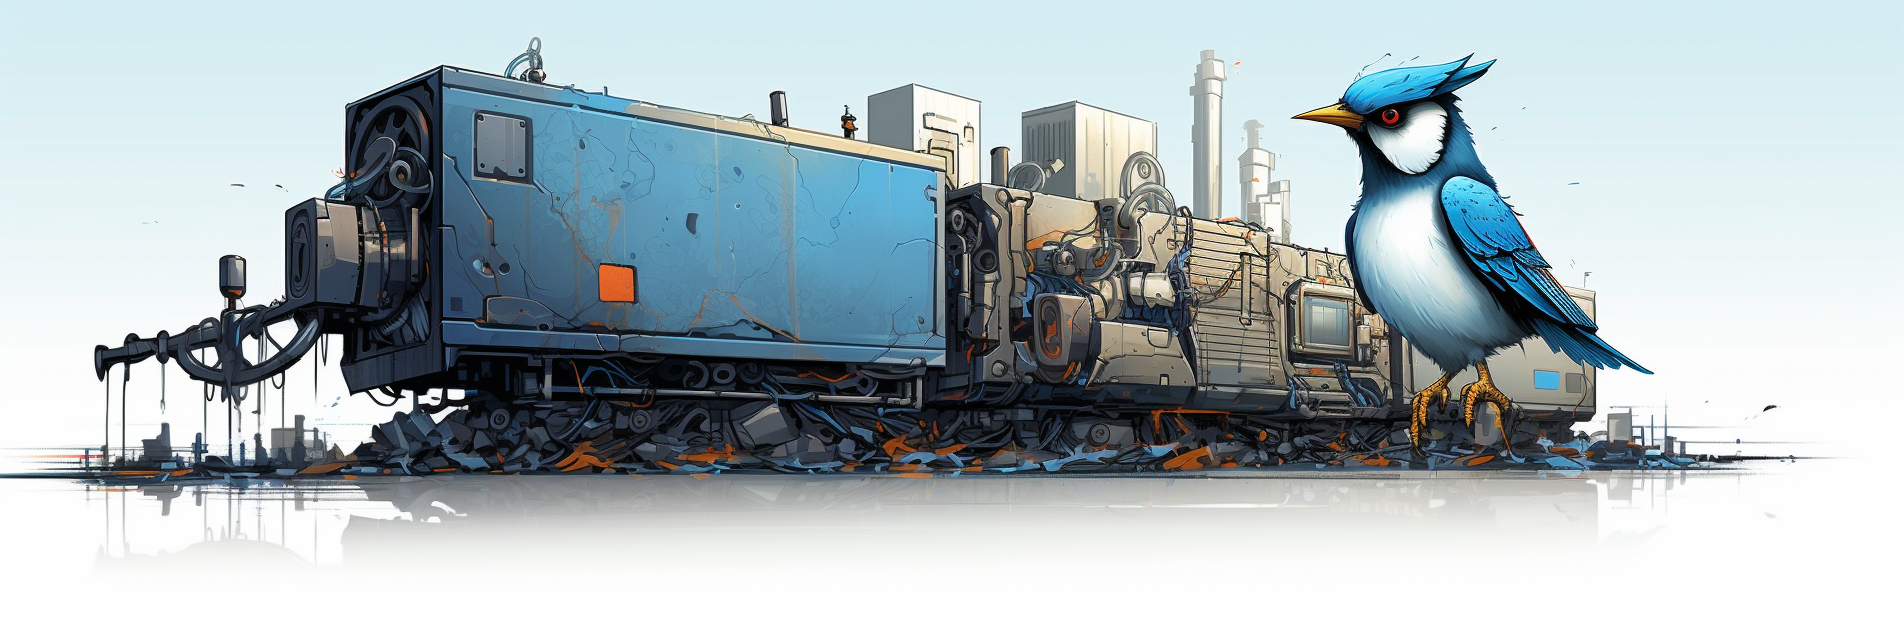
\includegraphics[width=\linewidth]{contents/01-introduction/figs/01-bird.png}
  \end{tcolorbox}
  \caption{An auto-generated image of ``a bird looking at a gigantic supercomputer, which consumes an enormous amount of energy, white background, 3:1 aspect ratio''.}
  \label{fig:intro:bird}
\end{figure}

\subsection{The Bayesian brain and the Free Energy principle}

It is well-documented that the human brain operates on approximately 20 watts of power
consumption \citep{raichle_appraising_2002} and it is estimated that the entire human body
consumes around 100 watts \citep{kovac_20_2010}.
In comparison, a typical halogen office light bulb consumes power ranging from 50 to 100
watts and a modern supercomputer power consumption can be as high as 60 megawatts\footnote{https://www.hpcwire.com/2021/09/08/how-argonne-is-preparing-for-exascale-in-2022/}.
Therefore, while engaging in real-time reasoning about how to maintain homeostasis through the
simultaneous processing of many sensory information sources, moving a heavy body through
space, and philosophizing about potential career perspectives, the human body consumes about the
same power as a stationary ceiling attachment.
Such an unparalleled level of energy efficiency is truly remarkable.

How does a body achieve this?
We do not know exactly, but there are some strong ideas. 
Amongst those ideas, the "Bayesian Brain" hypothesis suggests that the brain implements an approximate Bayesian
inference process to make sense of sensory information and perform cognitive tasks
\citep{doya_bayesian_2006}.
It suggests that the brain comprises a probabilistic model of its environment, continually
infers the likely causes of its sensorium, and updates its models on-the-fly when
prediction errors arise. 
But what is a probabilistic model and Bayesian inference?

\subsubsection{Probabilistic models and Bayesian inference}

A Bayesian inference process can be roughly described as \textit{learning about what we do not observe based on what we observe}.
In particular, the Bayesian approach provides a comprehensive mathematical framework for inference and statistical reasoning and describes a systematic way to update our prior beliefs and make informed decisions in the presence of uncertainty. 
Bayesian inference is often applied in reasoning together with \textit{probabilistic models}.
A probabilistic model $p(\bm{y}, \bm{s})$ is a structured representation of uncertainty and probabilistic relationships between observations $\bm{y}$ and hidden states $\bm{s}$. In this context \textit{``what we observe''} is $\bm{y}$ and \textit{``what we do not observe''} is $\bm{s}$.
Given a model $p(\bm{y}, \bm{s})$ and a set of new observations $\hat{\bm{y}}$, Bayesian inference uses Bayes rule to infer a posterior distribution $p(\bm{s}\vert\hat{\bm{y}})$, which represents our posterior beliefs about the hidden causes of these observations.
% \begin{equation}
%     \label{eq:intro:bayesrule}
%     \underbrace{p(\bm{s}\vert\bm{y})}_{\mathrm{posterior~beliefs}} \cdot \overbrace{\int p(\bm{y}\vert\bm{s})p(\bm{s})\mathrm{d}\bm{s}}^{\mathrm{evidence~}p(\bm{y})} = \underbrace{p(\bm{y}\vert\bm{s})}_{\mathrm{likelihood}}\cdot\overbrace{p(\bm{s})}^{\mathrm{prior~beliefs}}
% \end{equation}
\begin{figure}
  \centering
  \resizebox{1.0\textwidth}{!}{\begin{tikzpicture}[node distance=0.5mm, inner sep=0mm]
  %Nodes
  \node[] (eq) {$=$};
  \node[] (posterior) [left=of eq, yshift=0.25mm] {$p(\bm{s}\vert\hat{\bm{y}})$};
  \node[] (fractionleft) [right=of eq, yshift=0.25mm] {};
  \node[node distance=8mm] (fractioncenter) [right=of fractionleft] {};
  \node[node distance=8mm] (fractionright) [right=of fractioncenter] {};

  \path[-] (fractionleft.center) edge[] 
    node[pos=0.3, anchor=south, yshift=0.5mm](likelihood){$p(\hat{\bm{y}}\vert\bm{s})$}
    node[pos=0.8, anchor=south, yshift=0.5mm](prior){$p(\bm{s})$}
    node[pos=0.5, anchor=north, yshift=-0.5mm](evidence){$p(\hat{\bm{y}})$}
  (fractionright.center);

  \node[align=left] (posteriorcaption) [below=of posterior, yshift=-1mm, xshift=-17mm, align=left] {
  \begin{varwidth}{30mm}
      \small{Posterior}\\
      \tiny{probability distribution of the hidden states given observations} \\
      \tiny{\textit{(updated knowledge: how probable are hidden states given the observed data?)}}
    \end{varwidth}
  };

  \node[align=left] (likelihoodcaption) [above=of posterior, yshift=2mm, xshift=-15mm, align=left] {
  \begin{varwidth}{35mm}
      \small{Likelihood}\\
      \tiny{probability distribution for observed data, given hidden states. Since data is given, the likelihood is a function of states.} \\
      \tiny{\textit{(how ``likely'' are the states, given the data?)}}
    \end{varwidth}
  };

  \node[align=right] (priorcaption) [above=of posterior, yshift=0mm, xshift=46mm, align=right] {
  \begin{varwidth}{30mm}
      \small{Prior}\\
      \tiny{probability distribution of hidden states, before any observations} \\
      \tiny{\textit{(prior knowledge: how probable are the hidden states before observing any data?)}}
    \end{varwidth}
  };

  \node[align=right] (evidencecaption) [below=of posterior, yshift=-1mm, xshift=43mm, align=right] {
  \begin{varwidth}{35mm}
      \small{Evidence}\\
      \tiny{probability distribution of the observed data independently of the hidden states. Often interpreted  as a model score} \\
      \tiny{\textit{(how probable are these particular observations for this model?)}}
    \end{varwidth}
  };

  \draw (posteriorcaption.east) -| ([yshift=-1mm]posterior.south) node[pos=0.0, circle,fill=black,inner sep=0pt,minimum size=2pt]{} node[pos=1.0, circle,fill=black,inner sep=0pt,minimum size=2pt]{};

  \draw (likelihoodcaption.east) -| ([yshift=1mm]likelihood.north) node[pos=0.0, circle,fill=black,inner sep=0pt,minimum size=2pt]{} node[pos=1.0, circle,fill=black,inner sep=0pt,minimum size=2pt]{};

  \draw ([xshift=-1mm]priorcaption.west) -| ([yshift=1mm]prior.north) node[pos=0.0, circle,fill=black,inner sep=0pt,minimum size=2pt]{} node[pos=1.0, circle,fill=black,inner sep=0pt,minimum size=2pt]{};
  
  \draw ([xshift=-1mm]evidencecaption.west) -| ([yshift=-1mm]evidence.south) node[pos=0.0, circle,fill=black,inner sep=0pt,minimum size=2pt]{} node[pos=1.0, circle,fill=black,inner sep=0pt,minimum size=2pt]{};

\end{tikzpicture}}
  \caption{Schematic illustration of Bayes rule applied to the inference of hidden states $\bm{s}$ given actual observations $\hat{\bm{y}}$.}
  \label{fig:intro:bayesrule}
\end{figure}
In particular, in probabilistic models, the ``forward'' (generative) direction of the model describes how specific hidden states lead to observations and the ``backward'' (inference) direction relates to using the Bayes rule to derive the distribution over hidden states and update our prior beliefs for a given set of observations.
\begin{figure}
  \centering
  \resizebox{1.0\textwidth}{!}{\begin{tikzpicture}[]
  %Nodes
  \node[] (center) {};

  \node[box, fill=white] (model) {Probabilistic model~$p(\bm{y}, \bm{s})$};
  \node[box, minimum width=30mm] (prior) [left=of model]{Prior beliefs $p(\bm{s})$};
  \node[box, minimum width=30mm] (data) [right=of model]{Observations $p(\bm{y})$};

  \path[line, thick] (prior) edge[-] 
    node[pos=0.5](llinecenter){} 
    % node[pos=0.5, anchor=south](llinecentercaption){$\bm{s}$}
    (model);
  \path[line, thick] (model) edge[-] 
    node[pos=0.5](rlinecenter){} 
    % node[pos=0.5, anchor=south](rlinecentercaption){$\bm{y}$} 
    (data);

  \node[] (ltpivot) [above=of llinecenter, yshift=-5mm] {};
  \node[] (lbpivot) [below=of llinecenter, yshift=5mm] {};
  \node[] (rtpivot) [above=of rlinecenter, yshift=-5mm] {};
  \node[] (rbpivot) [below=of rlinecenter, yshift=5mm] {};

% $p(\bm{y}\vert\hat{\bm{s}}) = \frac{p(\hat{\bm{s}}\vert\bm{y})p(\bm{y})}{p(\hat{\bm{s}})}$
% $p(\bm{s}\vert\hat{\bm{y}}) = \frac{p(\hat{\bm{y}}\vert\bm{s})p(\bm{s})}{p(\hat{\bm{y}})}$

  \path[line, thick] (ltpivot) edge[-stealth] 
    node[pos=0.5, anchor=south]{Forward (generative)}
  (rtpivot);
  \path[line, thick] (rbpivot) edge[-stealth] 
    node[pos=0.5, anchor=north]{Backward (inference)}
  (lbpivot);
  
\end{tikzpicture}}
  \caption{Schematic illustration of an interaction between prior and actual observed information in a probabilistic model.
    In probabilistic models, the ``forward'' (generative) direction of the model describes how specific hidden states lead to observations and the ``backward'' (inference) direction relates to using the Bayes rule to derive the distribution over hidden states and update our prior beliefs for a given set of observations.
  }
  \label{fig:intro:bayesflow}
\end{figure}
The Bayesian approach finds extensive applications in signal processing \citep{bagautdinov_machine_2013}, healthcare \citep{lu_bayesian_2018}, forecasting \citep{berninger_bayesian_2020}, psychology \citep{wagenmakers_bayesian_2018}, and many more, and offers several advantages relative to non-Bayesian reasoning, such as
\begin{itemize}
    \item providing a coherent framework for incorporating prior knowledge and fusing information from
both prior and observed information;
    \item allowing for model comparison using the evidence terms from different models;
    \item providing interpretable results in the form of posterior distributions, which can be easily understood and communicated.
\end{itemize}
But how exactly can Bayesian inference help us to build intelligent agents?

\subsubsection{The Free Energy principle}

The Bayesian brain hypothesis aligns well with \ac{fep} \citep{friston_free_2006}.
According to \ac{fep}, any natural \textit{intelligent} agent (such as the brain) comprises a
model for the environmental causes of its sensorium and continually minimizes \ac{vfe} in that model \citep{sims_modelling_2021}, which is defined as:
\begin{equation}
    F[q] = \int q(\bm{s}) \log \frac{q(\bm{s})}{p(\bm{y}, \bm{s})} \mathrm{d}\bm{s},
\end{equation}
where $q(\bm{s})$ is a so-called variational distribution, which acts as an approximation to the Bayesian posterior $p(\bm{s}\vert\hat{\bm{y}})$.
In this context, \ac{fep} can be interpreted as the Principle of Least Action in biology and biotic behavior \citep{FRISTON20231}, and variational optimization of \ac{vfe} can be understood as an approximation to Bayesian inference \citep{friston_free-energy_2007}.

\begin{figure}
  \centering
  \resizebox{0.85\textwidth}{!}{\begin{tikzpicture}[]
  %Nodes
  \node[] (center) {};

  \node[inner sep=0pt, opacity=0.25] (brain)[right=of center, xshift=-3.5mm]{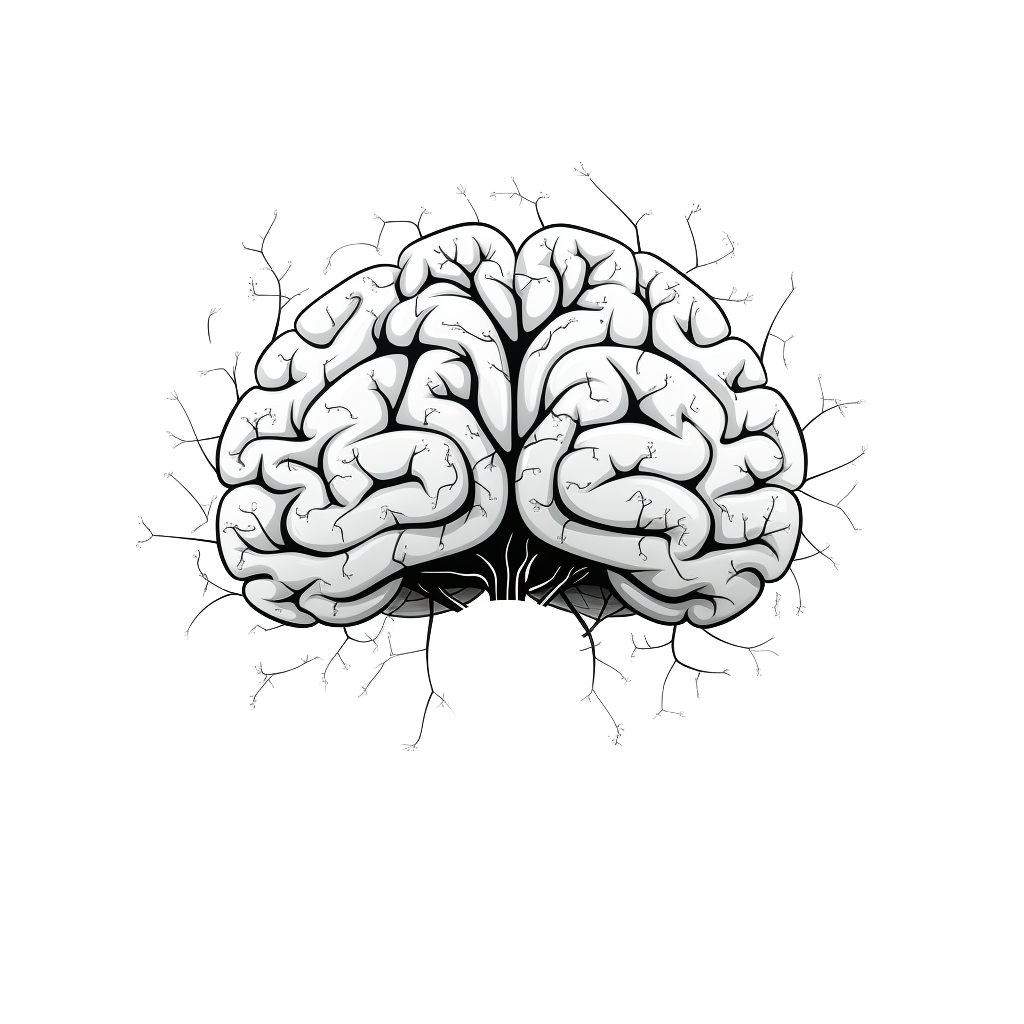
\includegraphics[width=.45\textwidth]{contents/01-introduction/figs/01-fep-brain.png}};
  \node[inner sep=0pt, opacity=0.25] (planet)[left=of center, xshift=3.5mm]{
\includegraphics[width=.45\textwidth]{contents/01-introduction/figs/01-fep-planet.png}};

  \node[box, minimum width=30mm, minimum height=10mm, fill=white](hidden)[left=of center, xshift=-10mm]{Hidden states};
  \node[box, minimum width=30mm, minimum height=10mm, fill=white](model)[right=of center, xshift=10mm]{Internal model};
  \node[box, minimum width=30mm, minimum height=10mm](sensory)[above=of center]{Sensory input};
  \node[box, minimum width=30mm, minimum height=10mm](actions)[below=of center]{Actions};

   \path[line, thick] (hidden) edge[out=90,in=180] node [] {} (sensory);
   \path[line, thick] (sensory) edge[out=0,in=90] node [] {} (model);
   \path[line, thick] (model) edge[out=270,in=0] node [] {} (actions);
   \path[line, thick] (actions) edge[out=180,in=270] node [] {} (hidden);

   \path[line, thick] (model) edge[out=180,in=270] node [] {} (sensory);
   \path[line, thick] (hidden) edge[out=0,in=90] node [] {} (actions);
   \path[line, thick, <->] (sensory) edge[out=270,in=90] node [] {} (actions);

\end{tikzpicture}}
  \caption{Schematic illustration of the reciprocal exchanges between an agent (on the right) and its environment (on the left).
    The hidden states of the environment are inferred using approximate posterior estimates within
    an internal model, which is conditioned on the activity of the agent's sensory receptors
    (sensory states).
    The internal states also infer the evolution of the agent's actuators (action states),
    enabling the agent to bring changes in the external states that align with the expected
    sensory states.
    The \acl{fep} states that the inference process in the internal model minimizes
    the \acl{vfe} in that model.
  }
  \label{fig:intro:fep}
\end{figure}

The concept that self-organizing biological systems, such as cells or brains, can be explained by their tendency to minimize \ac{vfe} is rooted in Helmholtz's work on unconscious inference \citep{helmholtz66, meyering_helmholtzs_1989} and has been further explored in psychology \citep{gregory_perceptions_1980} and machine learning \citep{dayan_helmholtz_1995}. 
Crucially, from an information processing viewpoint, \ac{vfe} minimization is the \textit{only}
ongoing process, and it is therefore responsible for all thought processes, learning,
decision-making, and ultimately, intelligent behavior.
In short, according to FEP, \textbf{the brain is a probabilistic model for sensory observations, and Bayesian inference in that model is the underlying process for natural intelligence}.

\subsection{Intelligent agents and the Active Inference framework}

\Ac{aif} is a corollary of \ac{fep} and describes how
natural agents might use \ac{vfe} minimization to infer potential future events and their next actions, in addition to the environmental causes of observations at the present time \citep{smith_step-by-step_2021, de_vries_factor_2017}.
If \ac{vfe} minimization in natural agents is responsible for intelligent reasoning and
decision making, the question arises if we can transfer these ideas to engineering and
consider the development of synthetic \ac{aif} agents that go out into the world and learn
purposeful behavior on-the-fly, without the need for a large training data set or reliance on
a power-hungry cluster of \acp{gpu}. And if we can, where should we start?

In fact, toy-sized \ac{aif} agents have already been designed and shown to work in practice
\citep{friston_active_2016,pio-lopez_active_2016,da_costa_active_2020,van_de_laar_active_2022, koudahl_realising_2023, van_de_laar_realising_2023},
however, the application of \ac{aif} for large-scale real-world problems remains a challenge.
The brain's exceptional computational capabilities for \ac{vfe} minimization include automated,
simultaneous (parallel), spontaneous (reactive), large-scale (billions of synapses),
time-varying processing of high-dimensional sensory data streams, in real time, under
ultra-low power (<20W) resource constraints.
Furthermore, the brain has the ability to adapt beliefs about environmental causes
(represented by model states) of new observations, update beliefs about model
parameters, and update the model structure over time under the pressure of minimizing
\ac{vfe}.

Sadly, there is no ``\ac{ai} software toolbox'' today that aims to support nature-inspired
intelligent agents solely through \ac{vfe} minimization, which makes it difficult to test these hypotheses in ``the field''. 
Motivated by \ac{fep}, this thesis is driven by the challenge of creating a practical software tool for Bayesian inference, 
where all processing stems from efficient \ac{vfe} minimization.
It is important to recognize that this work does not aim to provide a definitive solution to the complex problem of how intelligent synthetic agents should behave, learn, and be simulated. Instead, the goal is to take significant steps toward achieving these objectives. By exploring the principles and mechanisms proposed by \ac{fep} and \ac{aif}, this research contributes to the ongoing efforts of the research community and lays the foundation for further advancements.
% and eventually enabling the realization of synthetic \ac{aif} agents.
\section{Research questions}\label{chapter-01:section:questions}

%\subsection{Neuroscientist walks into an engineering bar}

%We now return to motivate the problem and discuss the challenges.
%We now return to the motivation of the problem.

The central research issue in this thesis is how to transfer ideas from the neuroscience community and \ac{fep} in particular to the design of useful engineering systems.
How can we design an intelligent system that works with a similar computational scheme (\ac{vfe} minimization) as the brain, and what are its essential components? If we embrace the principles of \ac{fep} and \ac{aif}, then we must also embrace Bayesian inference as the selected approach to reasoning and updating beliefs in the presence of new information.
However, what are the key ingredients for the realization of \ac{aif} agents through (approximate) Bayesian inference?
Once again, we draw inspiration from our understanding of the functioning of the brain.

The brain has dozens of billions of neurons \citep{herculano-houzel_human_2009}, therefore,
inference in such a large model must be \textbf{efficient} and \textbf{scalable}.
On the other hand, the brain loses thousands of neurons per day \citep{barrett_optimal_2016},
so inference in the brain must be \textbf{robust} and stay operational even under local failures.
The brain reacts in real-time, how else could we learn to ride a bike\footnote{tenzij je fietsen in je genen hebt zitten}? 
Therefore, inference in \ac{aif} agents must be \textbf{fast} and
\textbf{continual}.
The brain interacts in an environment that is constantly changing, consequently, inference
must \textbf{adapt} to changes \textbf{without interruption}.
The brain is lazy in the sense that it does not focus on (i.e. process) everything at the same time with the same attention.
Rather, the brain prioritizes important issues and updates beliefs with varying power budgets, varying precisions, and varying time scales.
%As a consequence, the inference process in the brain is \textbf{lazy} and infers only when necessary.

\begin{figure}
  \centering
  \resizebox{1.0\textwidth}{!}{\begin{tikzpicture}[node distance=1mm]
  %Nodes
  \node[box, minimum width=22mm] (realtime) {Real-time};
  \node[box, minimum width=22mm] (scalable) [right=of realtime] {Scalable};
  \node[box, minimum width=22mm] (robust) [right=of scalable] {Robust};
  \node[box, minimum width=22mm] (adaptive) [right=of robust] {Adaptive};
  
  \node[box, minimum width=22mm] (lazy) [below=of realtime] {Lazy};
  \node[box, minimum width=22mm] (versatile) [right=of lazy] {Versatile};
  \node[box, minimum width=22mm] (lowpower) [right=of versatile] {Low-power};
  \node[box, minimum width=22mm] (easytouse) [right=of lowpower] {Easy-to-use};

  \node[box, densely dotted] (bayes) [fit=(realtime)(easytouse)] {};
  \node[] (bayeslabel) [above=of bayes] {$\text{Approximate Bayesian inference}^*$};
  \node[box, inner xsep=5mm, inner ysep=3mm, rounded corners, minimum width=100mm] (bayesbox) [fit=(bayes)(bayeslabel)] {};
  
  \node[box, inner xsep=5mm, inner ysep=1mm, rounded corners, node distance=3mm, minimum width=80mm] (vfe) [above=of bayesbox] {
    Variational Free Energy minimization
  };

  \node[box, inner xsep=5mm, inner ysep=1mm, rounded corners, node distance=3mm, minimum width=80mm] (fep) [above=of vfe] {
    Free Energy Principle \& Active Inference
  };

  \node[box, inner xsep=5mm, inner ysep=1mm, rounded corners, node distance=3mm, minimum width=80mm] (nai) [above=of fep] {
    Natural Intelligent Behaviour
  };

  \draw[] (nai) edge[-stealth] (fep);
  \draw[] (fep) edge[-stealth] (vfe);
  \draw[] (vfe) edge[-stealth] (bayesbox);
  
  % \node[] (feplabel) [above=of fep] {Variational Free Energy minimization};

  % \node[box, inner xsep=5mm, inner ysep=3mm, rounded corners] (aif) [fit=(fep)(feplabel)] {};
  % \node[] (aiflabel) [above=of aif] {Free Energy Principle \& Active Inference};

  % \node[box, rounded corners, inner xsep=5mm, inner ysep=3mm, label={Natural Intelligent Behaviour}] (nai) [fit=(aif)(aiflabel)] {};

\end{tikzpicture}}
  \caption{
    Inspired by the powerful consequences of nature's principle of minimizing the \ac{vfe}
functional in the least amount of time, in this dissertation we are motivated by the challenge of
developing useful software tool for realizing synthetic \ac{aif} agents in which all processing follows 
from efficient \ac{vfe} minimization implemented as approximate, real-time, scalable and robust Bayesian inference. 
$\mathbin{^*\!~}$ In this dissertation we specifically focus on approximate Bayesian inference as a foundation for \ac{aif}.
  }
\end{figure}

Can we design a Bayesian inference framework that implements all of these properties? Specifically, in this thesis we aim to answer the following main question:

\newcommand{\mainquestion}{What is a suitable
  implementation for real-time, efficient, and robust Bayesian inference in a large-scale model for streaming data?
}

\begin{rqbox}
  \mainquestion
\end{rqbox}

Answering this question would be essential to design intelligent synthetic \ac{aif} agents that operate
continuously, act reactively, and learn autonomously.
It is worth noting that such an implementation would be useful not only for \ac{aif} agents but for
any application where real-time Bayesian inference is required, including audio processing,
self-driving vehicles, weather forecasting, extended reality video processing, and others.
Even though we take our motivation and inspiration from \ac{fep} and \ac{aif}, we are aware that progress on real-time, scalable  Bayesian inference may lead to an impact beyond the domain of synthetic \ac{aif} agents.
Therefore, our objective is to design a comprehensive Bayesian inference implementation for many related applications.
In particular, the work is driven by the following concrete research questions.

\newcommand{\scalabilityquestion}{
  How can Bayesian inference be efficiently realized in large multidimensional probabilistic
  generative models?
}

\begin{questions}
  \item \textbf{Scalability}. \scalabilityquestion
  \label{question:scalability}
\end{questions}

The world is a complex environment and any adequate probabilistic generative model of such an
environment would likely include thousands of variables.
The architecture for inference should scale comfortably to support large probabilistic models
that may involve both continuous and discrete states, as well as complex relationships between
these variables.

\newcommand{\reactivityquestion}{
  How can Bayesian inference be guaranteed to process streaming data in real-time?
}

\begin{questions}[resume] 
  \item \textbf{Real-time processing}. \reactivityquestion
  \label{question:reactivity}
\end{questions}

Bayesian inference in \ac{aif} agents in real-time applications should operate without "resetting" or "ending".
It should continuously incorporate new observations from streaming data, ensuring that
previously inferred information is not ignored.
This real-time processing of streaming data is essential for implementing an action-perception
control loop, where timely inference is crucial.
By linking the notion of real-time processing with streaming data, we must acknowledge the
dynamic nature of the real world and the need for continual Bayesian inference updates.

\newcommand{\robustnessquestion}{
  How can Bayesian inference continue without interruption under structural model adaptation?
}

\begin{questions}[resume]
  \item \textbf{Robustness}. \robustnessquestion
  \label{question:robustness}
\end{questions}

A real-world environment is prone to change and the existing structure of a probabilistic model may become suboptimal. 
As an intelligent agent interacts with its environment and collects new data, it seeks to update its probabilistic model structure to better capture the underlying patterns and dynamics of the observed phenomena.
There are situations, however, where changes in the probabilistic model occur unintentionally.
For instance, sudden failure or malfunction of a model component may be driven by a collision with another object. 
In these circumstances, it is crucial for the inference process to maintain operational continuity as much as possible.
The system should be designed to handle structural changes in the model.
This requires the ability to recover from failures, repair or update the model when necessary, and seamlessly continue the inference process without interruptions.

\newcommand{\userexperiencequstion}{
  How can we implement such a framework in a user-friendly manner?
}

\begin{questions}[resume]
  \item \textbf{User Experience}. \userexperiencequstion
  \label{question:user-experience}
\end{questions}

Consider popular machine learning frameworks such as \texttt{TensorFlow} or \texttt{PyTorch},
which have greatly simplified the implementation of Deep Learning (DL) models and made
them accessible to a wider audience.
These frameworks provide user-friendly interfaces, abstracting away many technical
complexities and allowing users to focus on model design and experimentation.
In the context of real-time Bayesian inference for autonomous intelligent agents, it is
crucial to present the implementation in a similarly user-friendly manner.
The focus on user experience is essential to reduce the required level of competence, thus allowing
a wider range of individuals to participate in the design and implementation of these
sophisticated systems.

\newcommand{\utilityquestion}{
  How can we support a wide range of probabilistic models and inference constraints?
}

\begin{questions}[resume]
  \item \textbf{Utility}. \utilityquestion
  \label{question:utility}
\end{questions}

Although it is possible to implement fast and robust real-time Bayesian inference for specific
models and specific applications, our objective is to create a universal approach that can universally accommodate
a wide range of probabilistic models and inference constraints.
By addressing this broader scope, we aim to develop a versatile framework that provides
practical utility and extends its applicability beyond specific use cases.


\section{Solution approach}\label{chapter-01:section:discussion}

Here, we discuss the solution approach for Bayesian inference as a foundation for \ac{aif} and explore the need for a new architecture specifically designed for real-time processing of streaming data.

% While Bayesian reasoning has a long and extensive research history, there are limitations that necessitate a new approach.

\subsection{Why is Bayesian inference so challenging?}

One of the fundamental challenges in probabilistic modeling is evaluating the posterior distribution of hidden states given observations, see Figure~\ref{fig:intro:bayesrule}. 
According to Bayes rule, computing the posterior involves three terms: a prior, a likelihood, and an evidence term. 
The first two can be easily expressed, as they are part of the assumed model $p(\bm{y}, \bm{s})$, and, in many situations, the prior and the likelihood are explicitly known. 
However, the evidence term, a normalization factor, requires to be computed such that 
\begin{equation}
    p(\bm{y}) = \int p(\bm{y}\vert\bm{s})p(\bm{s})\mathrm{d}\bm{s},
\end{equation}
where the integration is replaced with summation in the case of discrete variables.
In low dimensions, this integral can be computed relatively easily. However, in higher dimensions, the exact computation of the posterior distribution often becomes unfeasible. This challenge is further compounded when dealing with continuous variables or summing over exponentially many hidden states in discrete variables. To address these challenges, approximation techniques are often employed to compute or approximate the posterior distribution.

\subsection{Existing implementations of Bayesian inference}

Modern automated approximate Bayesian inference methods can be broadly categorized into two major categories, namely \textbf{sampling}-based and \textbf{variational}-based inference methods. 

\begin{figure}
  \centering
  \resizebox{1.0\textwidth}{!}{\begin{tikzpicture}[node distance=1mm, inner sep=0mm]

  \node[box, inner ysep=1mm, inner xsep=4mm, rounded corners, minimum height=5mm] (bayes) {\scriptsize Approximate Bayesian inference};

    \node[box, inner sep=1mm, minimum height=5mm, rounded corners, minimum width=20mm] (sampling) [below=of bayes,  xshift=-30mm, yshift=-2mm] {\scriptsize Sampling};
  \node[box, inner sep=1mm, minimum height=5mm, rounded corners, minimum width=20mm] (variational) [below=of bayes,yshift=-2mm] {\scriptsize Variational};
  \node[box, inner sep=1mm, minimum height=5mm, rounded corners, minimum width=20mm] (others1) [below=of bayes, xshift=30mm, yshift=-2mm] {\scriptsize $\cdots$};

  \node[box, inner sep=1mm, minimum height=3.5mm, rounded corners, minimum width=15mm] (blackboxvariational) [below=of variational, yshift=-2mm, xshift=-7mm] {\scriptsize Black-box};

  \draw (bayes) -- (variational);
  \draw (bayes) -- (sampling);
  \draw (bayes) -- (others1);

  \node[box, inner sep=1mm, minimum height=3.5mm, rounded corners, minimum width=7mm] (hmc) [below=of sampling, xshift=-18mm, yshift=-2mm] {\tiny HMC};
  \node[box, inner sep=1mm, minimum height=3.5mm, rounded corners, minimum width=7mm] (nuts) [right=of hmc] {\tiny NUTS};
  \node[box, inner sep=1mm, minimum height=3.5mm, rounded corners, minimum width=7mm] (pg) [right=of nuts] {\tiny PG};
  \node[box, inner sep=1mm, minimum height=3.5mm, rounded corners, minimum width=7mm] (other3) [right=of pg] {\tiny $\cdots$};

  \draw (sampling) -- (hmc);
  \draw (sampling) -- (nuts);
  \draw (sampling) -- (pg);
  \draw (sampling) -- (other3);

  \node[box, inner sep=1mm, minimum height=3.5mm, rounded corners, minimum width=7mm] (advi) [below=of blackboxvariational, xshift=-15mm, yshift=-2mm] {\tiny ADVI};
  \node[box, inner sep=1mm, minimum height=3.5mm, rounded corners, minimum width=7mm] (bbvi) [right=of advi] {\tiny BBVI};
  \node[box, inner sep=1mm, minimum height=3.5mm, rounded corners, minimum width=7mm] (cvi) [right=of bbvi] {\tiny CVI};
    \node[box, inner sep=1mm, minimum height=3.5mm, rounded corners, minimum width=7mm] (other2) [right=of cvi] {\tiny $\cdots$};
  
  \node[box, inner sep=1mm, minimum height=3.5mm, rounded corners, minimum width=7mm] (vmp) [right=of blackboxvariational] {\tiny VMP};
  \node[box, inner sep=1mm, minimum height=3.5mm, rounded corners, minimum width=7mm] (other4) [right=of vmp] {\tiny $\cdots$};

  \draw (blackboxvariational) -- (advi);
  \draw (blackboxvariational) -- (bbvi);
  \draw (blackboxvariational) -- (cvi);
  \draw (blackboxvariational) -- (other2);
  
  \draw (variational) -- (blackboxvariational);
  \draw (variational) -- (vmp);
  \draw (variational) -- (other4);
  
\end{tikzpicture}}
  \caption{
Two major categories for approximate Bayesian inference. Sampling-based approaches generate samples from the posterior distribution to estimate expectations and compute summary statistics. These methods rely on random sampling to explore the posterior distribution and can provide asymptotically exact results given infinite computational resources. On the other hand, variational inference is an optimization-based approach that approximates the true posterior distribution with a simpler parametric distribution. It formulates the inference problem as an optimization problem and finds the best approximation within a specific class of distributions.
  }
  \label{fig:intro:approximate-bayes-methods}
\end{figure}

\subsubsection{Sampling-based Bayesian inference}

Sampling-based methods, such as \ac{nuts}, \ac{hmc}, and \ac{pg}, offer a generic and flexible approach to Bayesian inference, allowing inference across large class of probabilistic models. These methods rely on extensive \ac{mcmc} simulations or sampling techniques to draw samples from a partially normalized probability distribution. 
% The counterintuitive fact that we can obtain samples from a distribution that is not well normalized comes from the specific way we define the algorithm that is not sensitive to these normalization factors.
The resulting samples are then used to compute various useful statistics such as mean, standard deviation, and covariance, effectively circumventing the challenges posed by intractable posterior computations. 
\begin{figure}
  \centering
  \resizebox{1.0\textwidth}{!}{\begin{tikzpicture}[]

  \node[] (posteriorlabel) at (3.5,3.7) {\Huge $p(\bm{s}\vert\hat{\bm{y}}) \propto p(\hat{\bm{y}}\vert\bm{s})p(\bm{s})$};
  
  \draw [red, xshift=4cm, thick, fill=red!05!white] plot [smooth, tension=0.9] coordinates { (-2,0) (-1,0.1) (0,0.8) (1,1) (2,3) (3,0.5) (4,4) (5, 0.5) (6,0.3) (7,0)};

  \draw [gray, xshift=4cm, fill=gray!05!white] plot [smooth, tension=0.9] coordinates { (8,0) (9,0.1) (10,0.8) (11,1) (12,3) (13,0.5) (14,4) (15, 0.5) (16,0.3) (17,0)};

  \node[circle,fill=red,inner sep=0pt,minimum size=5pt] () at (13, 0.0) {};
  \node[circle,fill=red,inner sep=0pt,minimum size=5pt] () at (14, 0.0) {};
  \node[circle,fill=red,inner sep=0pt,minimum size=5pt] () at (14.2, 0.0) {};
  \node[circle,fill=red,inner sep=0pt,minimum size=5pt] () at (15, 0.0) {};
  \node[circle,fill=red,inner sep=0pt,minimum size=5pt] () at (15.6, 0.0) {};
  \node[circle,fill=red,inner sep=0pt,minimum size=5pt] () at (15.75, 0.0) {};
  \node[circle,fill=red,inner sep=0pt,minimum size=5pt] () at (15.8, 0.0) {};
  \node[circle,fill=red,inner sep=0pt,minimum size=5pt] () at (15.9, 0.0) {};
  \node[circle,fill=red,inner sep=0pt,minimum size=5pt] () at (16.5, 0.0) {};
  \node[circle,fill=red,inner sep=0pt,minimum size=5pt] () at (17.1, 0.0) {};
  \node[circle,fill=red,inner sep=0pt,minimum size=5pt] () at (17.4, 0.0) {};
  \node[circle,fill=red,inner sep=0pt,minimum size=5pt] () at (17.5, 0.0) {};
  \node[circle,fill=red,inner sep=0pt,minimum size=5pt] () at (17.6, 0.0) {};
  \node[circle,fill=red,inner sep=0pt,minimum size=5pt] () at (18.0, 0.0) {};
  \node[circle,fill=red,inner sep=0pt,minimum size=5pt] () at (18.1, 0.0) {};
  \node[circle,fill=red,inner sep=0pt,minimum size=5pt] () at (18.2, 0.0) {};
  \node[circle,fill=red,inner sep=0pt,minimum size=5pt] () at (18.3, 0.0) {};
  \node[circle,fill=red,inner sep=0pt,minimum size=5pt] () at (18.4, 0.0) {};
  \node[circle,fill=red,inner sep=0pt,minimum size=5pt] () at (20.0, 0.0) {};
  \node[circle,fill=red,inner sep=0pt,minimum size=5pt] () at (20.1, 0.0) {};

  \path[thick] (9,2) edge[-stealth] node[pos=0.5, anchor=south, yshift=5mm]{
  \begin{varwidth}{65mm}
    \LARGE Sampling from an unnormalized distribution
  \end{varwidth}
  } (15,2);

  \path[thick] (19,2) edge[-stealth] node[pos=0.5, anchor=south, yshift=5mm]{
  \begin{varwidth}{50mm}
    \LARGE Statistics/estimations from the samples
  \end{varwidth}
  } (24,2);

  \node[align=left] (meanlabel) at (28,3) {\Huge $\mu \equiv \mathop{\mathbb{E}}_{p(\bm{s}\vert\hat{\bm{y}})}\left[\bm{s}\right]$};
  \node[align=left] (varlabel) at (29.2,1.5) {\Huge $\sigma^2 \equiv \mathop{\mathbb{E}}_{p(\bm{s}\vert\hat{\bm{y}})}\left[(\bm{s} - \mu)^2\right]$};
  
\end{tikzpicture}}
  \caption{
Sampling-based methods rely on extensive \ac{mcmc} simulations or sampling techniques to draw samples from a partially normalized probability distribution. 
The resulting samples are then used to compute various useful statistics such as mean, standard deviation, and covariance, effectively circumventing the challenges posed by intractable posterior computations. 
  }
  \label{fig:intro:sampling-explained}
\end{figure}
Although widely used and effective in many scenarios, this approach also has its limitations \citep{betancourt_conceptual_2018}:
\begin{itemize}
    \item \textbf{Computational load}. The inference process in sampling-based methods is, generally, time-consuming, and may run for hours or even days.
    \item \textbf{Limited scalability}. Does not scale well to large high-dimensional problems and may be affected by the curse of dimensionality.
    \item \textbf{Limited adaptivity}. Lacks the ability to be adapted during the process. In case of small modifications to the model structure, the entire inference procedure must be stopped and restarted.
    \item \textbf{High power consumption}. Typically, requires powerful hardware (e.g. \acp{gpu}) for efficient execution \citep{henriksen_parallel_2012, terenin_gpu-accelerated_2019} and, as a consequence, tends to consume a significant amount of energy.
    \item \textbf{How many samples}? Choosing the effective sample size might be difficult and requires careful analysis for each specific model \citep{morita_determining_2008}.
    \item \textbf{Sensitivity to algorithm hyper-parameters}. Sensitive to the choice of algorithm parameters, such as step sizes or proposal distributions, which may require careful tuning.
    \item \textbf{Requires post-analysis}. Requires careful convergence analysis and verification by domain experts.
\end{itemize}

In conclusion, while sampling-based methods offer a generic and versatile approach to Bayesian inference, they are not well suited for use in real-time and continual Bayesian inference. High computational demand, limited scalability, high power consumption, and lack of adaptability are significant limitations for \ac{aif} agents. These limitations, which will be further demonstrated in the experiments in Chapter~\ref{chapter-05}, make it practically impossible to utilize and deploy sampling-based approaches in real-world scenarios where computational resources, efficiency, and adaptivity are crucial. 

\subsubsection{Black-box variational Bayesian inference}

\Ac{bbvi} and \ac{advi} are popular alternatives to sampling-based methods \citep{ranganath_black_2014, kucukelbir_automatic_2017}.
\Ac{vi} methods approach the inference task as an optimization problem, with the aim of finding an approximate solution due to the inherent complexity of the original problem. These methods introduce constraints that simplify the problem statement while maintaining sufficient accuracy for a specific application. By carefully selecting these constraints, \ac{vi} strikes a balance between computational efficiency and the quality of the approximation.
Variational methods offer better scalability for large models compared to sampling-based approaches and provide a generic method to perform inference in a wide range of probabilistic models.
However, the naive application of \ac{bbvi} or \ac{advi} to large-scale real-time applications faces certain challenges:
\begin{itemize}
    \item \textbf{Incompatibility with discrete states}. \ac{advi} is based on \ac{ad} techniques and is not compatible with discrete-valued states in the model.
    \item \textbf{Incorrect derivatives}. Automatically-generated derivatives can produce incorrect results \citep{beck_if-problem_1994}. And this is not just a bug in a particular implementation but one of the fundamental limitations of modern \ac{ad} systems.
    \item \textbf{Sub-optimal derivatives}. Automatically-generated derivatives can be sub-optimal in terms of the usage of computational resources (in some cases, however, automatically generated derivatives are as fast as handwritten equivalents).
    \item \textbf{Limited adaptivity}. Both \ac{bbvi} and \ac{advi} treat the entire inference procedure as a black box, which limits the ability to adapt the structure of the model over time or adjust small parts of the inference procedure. In case of small modifications to the model structure, the entire inference procedure must be stopped and restarted.
    \item \textbf{Does not leverage the model structure}. In addition to the previous one, the black-box treatment of the model structure cannot fully exploit independence assumptions and conjugate relationships between variables, leading to sub-optimal inference performance in many scenarios.
\end{itemize}

These limitations make it difficult to use these particular implementations of \ac{vi}, such as \ac{bbvi} and \ac{advi}, for real-time Bayesian inference for streaming datasets. However, the approach itself offers a promising direction, as it allows one to directly control computational load and approximation accuracy. 

\begin{figure}
  \centering
  \resizebox{1.0\textwidth}{!}{\begin{tikzpicture}[]

  \node[] (posteriorlabel) at (3.5,2.7) {\Huge $p(\bm{s}\vert\hat{\bm{y}})$};
  \node[] (variationallabel) at (22,2.7) {\Huge $q(\bm{s})$};
  
  \draw [red, xshift=4cm, thick, fill=red!05!white] plot [smooth, tension=0.9] coordinates { (-2,0) (-1,0.1) (0,0.8) (1,1) (2,3) (3,0.5) (4,4) (5, 0.5) (6,0.3) (7,0)};

  \draw [gray, xshift=4cm, fill=gray!05!white] plot [smooth, tension=0.9] coordinates { (10,0) (11,0.1) (12,0.8) (13,1) (14,3) (15,0.5) (16,4) (17, 0.5) (18,0.3) (19,0)};

  \path[thick] (10,2) edge[-stealth] node[pos=0.5, anchor=south, yshift=3mm]{
  \begin{varwidth}{70mm}
    \Large Approximate with a ``simple'' distribution
  \end{varwidth}
  } (16,2);

  \draw [blue, xshift=4cm, fill=blue!15!white, opacity=0.65] plot [smooth, tension=0.6] coordinates { (11,0.005) (12,0.15) (13,0.9) (14,3) (15,0.9) (16,0.15) (17,0.005)};

  \draw [teal, xshift=4cm, fill=teal!15!white, opacity=0.65] plot [smooth, tension=0.6] coordinates { (13,0.005) (14,0.15) (15,0.9) (16,4) (17,0.9) (18,0.15) (19,0.005)};
  
\end{tikzpicture}}
  \caption{
\Ac{vi} methods approach the inference task as an optimization problem, aiming to find an approximate solution $q(\bm{s})$ due to the inherent complexity of the original problem of computing $p(\bm{s}\vert\hat{\bm{y}})$. These methods introduce constraints that simplify the problem statement while maintaining sufficient accuracy for a specific application. By carefully selecting these constraints, \ac{vi} strikes a balance between computational efficiency and the quality of the approximation.
  }
  \label{fig:intro:variational-explained}
\end{figure}

\subsubsection{The need for an alternative approach}

\begin{table}
\centering
\begin{tabular}{|l|| C{25mm} | C{25mm} |} 
 \hline
 \diagbox{Criteria}{Method} & Sampling & Black-box VI \\ [0.5ex] 
 \hline\hline
 Universal & \cellcolor[HTML]{dfffdf} \tikzcmark & \cellcolor[HTML]{dfffdf} \tikzcmark \\ \hline
 Automated & \cellcolor[HTML]{dfffdf} \tikzcmark & \cellcolor[HTML]{dfffdf} \tikzcmark \\ \hline
 Scalable & \cellcolor[HTML]{ffdfdf} \tikzxmark & \cellcolor[HTML]{dfffdf} \tikzcmark \\ \hline
 Real-time & \cellcolor[HTML]{ffdfdf} \tikzxmark & \cellcolor[HTML]{ffdfdf} \tikzxmark \\ \hline
 Adaptable & \cellcolor[HTML]{ffdfdf} \tikzxmark & \cellcolor[HTML]{ffdfdf} \tikzxmark\\ \hline
 Continual & \cellcolor[HTML]{ffdfdf} \tikzxmark & \cellcolor[HTML]{ffdfdf} \tikzxmark  \\ \hline
 Low-power & \cellcolor[HTML]{ffdfdf} \tikzxmark & \cellcolor[HTML]{ffdfdf} \tikzxmark  \\
 \hline
\end{tabular}
\caption{A (superficial) comparison of popular methodologies for approximate Bayesian inference.
Neither sampling-based (\ac{nuts}, \ac{hmc}, \ac{pg}) nor black-box variational (\ac{bbvi}, \ac{advi}) inference were designed to support fast and continual inference, model adaptation and real-time interaction under low-power. 
The computational demands and time-consuming nature of these methods can hinder their ability
to perform inference efficiently in real time on low-power devices.
Additionally, their lack of flexibility in model adaptation restricts their applicability in
scenarios where the probabilistic model needs to be continuously adjusted based on new
observations.
}
\label{table:intro:comparison}
\end{table}

Neither sampling-based (\ac{nuts}, \ac{hmc}, \ac{pg}) nor black-box variational (\ac{bbvi}, \ac{advi}) inference were designed to support fast and continual inference, real-time interaction, model adaptation, and updates at different time scales for different parts of probabilistic models.
While sampling-based methods and black-box variational inference have their merits and are
valuable in various applications, their inherent limitations make them less suitable for running real-time Bayesian inference in autonomous agents under situated conditions.
These methods do not meet the requirements for executing Bayesian inference in dynamic
environments.
The computational demands and time-consuming nature of these methods can hinder their ability
to perform inference efficiently in real time on low-power devices.
Additionally, their lack of flexibility in model adaptation restricts their applicability in
scenarios where the probabilistic model needs to be continuously adjusted based on new
observations.

To address these limitations, a new architecture for Bayesian inference is necessary, one that
is specifically tailored to the requirements of large-scale real-time applications.
This architecture should enable fast and continual inference, support real-time interaction
with the environment, facilitate model adaptation in response to changing conditions, and
allow for lazy updates to optimize computational resources.
By developing such an architecture, we can overcome the limitations of existing methods and
enable Bayesian inference to perform intelligent and adaptive behaviors in real-world
scenarios.

\subsection{Variational Bayesian inference}

% The techniques mentioned previously, BBVI and ADVI, are instances of \ac{vi}, which approaches the Bayesian inference problem as an optimization task subject to some constraints.
% In variational inference, which will be discussed in more details in Chapter~\ref{chapter-02},
% a variational distribution (also known as a recognition distribution) is introduced as an
% approximation to the true posterior.

\Ac{vi}, despite the described limitations, offers a promising direction, since it severely reduces the computational load associated with the inference problem, although it results in an approximate solution. This trade-off seems reasonable, considering that natural brains do not reason perfectly all the time and can make mistakes as a result of limitations on available computational resources. We discuss \ac{vi} in more detail in Chapter~\ref{chapter-02}, but the highlighted advantages are:
\begin{itemize}
    \item \textbf{Computational trade-off}. In situations where sufficient computational power is available, a larger search space can be
explored, allowing for increased computational load and potentially more accurate solutions;
    \item \textbf{Accuracy trade-off}. Conversely, when computational resources are limited, it becomes necessary to constrain the precision of computation and obtain solutions that may be less accurate but still enable real-time inference;
    \item \textbf{Potential scalability}. Choosing optimal optimization constraints might be a difficult task, but, if done correctly, it allows great scalability for large probabilistic models with millions of hidden states.
\end{itemize}

In addition, the approach aligns well with \ac{fep}, where the goal is to minimize \ac{vfe} by optimizing the variational distribution.
By adopting \ac{vi}, our objective is to strike a balance between computational
efficiency and inference quality, allowing the implementation of real-time inference in
large-scale probabilistic models.
This approach acknowledges the computational constraints of Bayesian inference operating in
dynamic environments while providing means to perform inference effectively and adaptively
within the available computational resources.
But how do we implement \ac{vi} so that it does not suffer from the limitations of the techniques mentioned above, such as \ac{bbvi} and \ac{advi}? 


\subsection{Probabilistic graphical models and factor graphs}

\Ac{vi}, regardless of its complexity, relies on variational calculus. 
Therefore, the solution to \ac{vi} in complex probabilistic models can be expressed using
pure algebra \citep{blei_variational_2017}.
However, it is possible to enhance algebraic manipulations with diagrammatic representations
known as \acp{gm}. 
A typical \ac{gm} consists of a graph composed of nodes and edges,
although the interpretation of these nodes and edges can vary depending on the specific \ac{gm}.
These graph-based \acp{gm} provide several useful properties in the context of Bayesian inference \citep[Ch.8]{bishop_pattern_2006}:
\begin{itemize}
\item \textbf{Not a black-box}. They provide insights into the properties of probabilistic models, such as conditional independence relationships;
  \item \textbf{Intuitive}. They offer a simple and intuitive way to visualize, interpret, and motivate the structure of a probabilistic model;
  \item \textbf{Local}. Different parts of the model can be easily analyzed, and adapted locally, without affecting the structure as a whole.
\end{itemize}

In the current dissertation, we extensively use a specific instance of \ac{gm}, which is called a \ac{fg}. 
\Acp{fg} are computational graphs that provide a convenient framework for expressing complex algebraic computations required for Bayesian inference through graphical manipulations.
Importantly, these graphical manipulations are performed locally, meaning that individual parts of the
factor graph can be modified without disrupting the inference in other parts of the graph.
By adopting \ac{gm}, our objective is to take advantage of the structure of the model, to be able to adapt the model dynamically and to avoid the associated issues with the black-box treatment of the inference procedure.
But what exactly are these graphical manipulations and why they might be useful?

\begin{figure}
  \centering
  \begin{subfigure}[t]{0.450\textwidth}
    \centering
    \resizebox{\textwidth}{!}{\begin{tikzpicture}[node distance=10mm]

  \node[box, circle, thick, minimum size=5mm, label=above left:{Object}] (object) {};
  \node[box, circle, thick, minimum size=5mm, label=above:{Position}] (position) [right=of object] {};
  \node[box, circle, thick, minimum size=5mm, label=above right:{Orientation}] (orientation) [right=of position] {};

  \node[box, circle, thick, minimum size=5mm, label=below:{Image}] (image) [below=of position] {};

  \path[line, thick] (object) edge[-stealth] (image);
  \path[line, thick] (position) edge[-stealth] (image);
  \path[line, thick] (orientation) edge[-stealth] (image);
  
\end{tikzpicture}}
    \caption{A directed graphical model, which is also known as Bayesian Network.}
    \label{fig:intro:gm_simple}
  \end{subfigure}
  \hfill
  \begin{subfigure}[t]{0.450\textwidth}
    \centering
    \resizebox{\textwidth}{!}{\begin{tikzpicture}[node distance=15mm]

  \node[box, thick, minimum size=10mm] (pobject) {$p_{1}$};
  \node[box, thick, minimum size=10mm] (pposition) [right=of pobject] {$p_{2}$};
  \node[box, thick, minimum size=10mm] (porientation) [right=of pposition] {$p_{3}$};

  \node[box, circle, thick, minimum size=5mm, label=right:{Object}, node distance=5mm] [below=of pobject] (object) {};
  \node[box, circle, thick, minimum size=5mm, label=right:{Position}, node distance=5mm] (position) [below=of pposition] {};
  \node[box, circle, thick, minimum size=5mm, label=right:{Orientation}, node distance=5mm] (orientation) [below=of porientation] {};

  \node[box, thick, minimum size=10mm, node distance=5mm] (pimage) [below=of position] {$p_{4}$};

  \node[box, circle, thick, minimum size=5mm, label=below:{Image}, node distance=5mm] (image) [below=of pimage] {};

  \path[line, thick] (pobject) edge[-] (object);
  \path[line, thick] (pposition) edge[-] (position);
  \path[line, thick] (porientation) edge[-] (orientation);
  \path[line, thick] (object) edge[-] (pimage);
  \path[line, thick] (position) edge[-] (pimage);
  \path[line, thick] (orientation) edge[-] (pimage);
  \path[line, thick] (pimage) edge[-] (image);
  
\end{tikzpicture}}
    \caption{An undirected graphical model in the form of a factor graph.}
    \label{fig:intro:gm_fg}
  \end{subfigure}
  \caption{A simple graphical probabilistic model $p(\mathrm{Object}, \mathrm{Position}, \mathrm{Orientiation}, \mathrm{Image}) = p_1(\mathrm{Object})p_2(\mathrm{Position})p_3(\mathrm{Orientiation})p_4(\mathrm{Image}\vert\mathrm{Object}, \mathrm{Position}, \mathrm{Orientiation})$ describing the process by which images of objects are created. $p_1, p_2, p_3$ represent prior probabilities and $p_4$ represents a likelihood function. The image (vector of pixels) has a probability distribution that depends on the identity of the object as well as on its position and orientation.}
  \label{fig:intro:gm}
\end{figure}


% In our work, we focus primarily on Forney-style factor graphs (FFGs), where each node is
% associated with individual factors and each edge is associated with an individual variable
% \citep{forney_codes_2001}. \bdv{It makes no sense to talk about "where each node is
% associated with individual factors ..." without context of what a factor is. Reader who dont know what a FFG is are not helped by an introduction full of jargon without an example graph, and readers who do know FFGs are bored. }
% However, the ideas and solutions presented can be extended to other representations of factor
% graphs.
% By expressing Bayesian inference as local computations on the factor graph representation, we
% leverage the advantages of locality, allowing for efficient and adaptable inference procedures
% within the model.

\subsection{Variational message passing on factor graphs}

\Ac{vi}, when applied in the context of factor graphs, offers an elegant interpretation that relies on the exchange of messages between factor nodes along the graph's edges, which is called \ac{vmp}. These messages carry all the necessary information about the rest of the graph, allowing efficient computation of variational posterior distributions \citep{dauwels_variational_2007}, but also has many other valuable properties:
\begin{itemize}
    \item \textbf{Parallel}. Messages can be exchanged in a parallel and scalable manner, capitalizing on the graph's structure and the conditional independence relationships encoded within it;
    \item \textbf{Local}. Messages can be examined and analyzed independently, focusing on their specific properties without dependence on the entire model structure;
    \item \textbf{Modular}. The approach enables the design of modular "building blocks" in the form of \acp{fg}, which can be
reused across various contexts and probabilistic models;
    \item \textbf{Lazy}. In principle, the approach allows for the transmission of messages at different frequencies,
which paves the way for performing lazy computations in different parts of the graph.
\end{itemize}

\begin{figure}
  \centering
  \resizebox{1.0\textwidth}{!}{\begin{tikzpicture}[node distance=5mm, style]

\tikzset{var/.style={box, circle, inner sep=0mm, minimum size=3mm}}

  \node[box] (b1) {};
  \node[var] (b2) [right=of b1] {};
  \node[box, draw=white] (b3) [right=of b2] {};
  \node[var] (b4) [right=of b3] {};
  \node[box] (b5) [right=of b4] {};

  \node[var] (b56) [below=of b3] {};
  \node[box] (b6) [right=of b56] {};
  \node[var] (b7) [right=of b6] {};
  \node[box] (b8) [right=of b7] {};
  \node[var] (b9) [above=of b8] {};

  \node[var] (b11) [below=of b1] {};
  \node[box] (b14) [right=of b11] {};

  \path[line] (b1) edge[-] node[pos=0.5, anchor=south]{\tiny $\rightarrow$} (b2);
  \path[line] (b2) edge[-] node[pos=0.5, anchor=south, rotate=270]{\tiny $\rightarrow$} (b14);
  \path[line] (b1) edge[-] (b11);
  \path[line] (b11) edge[-] node[pos=0.5, anchor=north]{\tiny $\rightarrow$} (b14);

  \path[line] (b14) edge[-] node[pos=0.5, anchor=south]{\tiny $\rightarrow$} (b56);
  \path[line] (b56) edge[-] node[pos=0.5, anchor=south]{\tiny $\leftarrow$} (b6);
  \path[line] (b6) edge[-] (b7);
  \path[line] (b7) edge[-] node[pos=0.2, anchor=south]{\tiny $\leftarrow$} node[pos=0.7, anchor=south]{\tiny $\leftarrow$} node[pos=0.5, anchor=north](freqmessages){} (b8);
  \path[line] (b8) edge[-] (b9);
  \path[line] (b4) edge[-] node[pos=0.5, anchor=south]{\tiny $\leftarrow$}  (b5);
  \path[line] (b5) edge[-] node[pos=0.5, anchor=south](parallelmessage){\tiny $\rightarrow$} node[pos=0.5, anchor=north]{\tiny $\leftarrow$}  (b9);
  \path[line] (b6) edge[-] (b4);

  \node[box, densely dotted] (reused) [fit=(b1)(b2)(b11)(b14)] {};
  \node[node distance=5mm] (reusedlabel) [above=of reused, xshift=-15mm] {
  \begin{varwidth}{25mm}
    \scriptsize \textbf{Modular}\\
    \tiny Sub-models can be reused across different probabilistic models
  \end{varwidth}
  };
  \draw (reusedlabel.east) -| ([xshift=5mm, yshift=1mm]reused.north) node[pos=0.0, circle,fill=black,inner sep=0pt,minimum size=2pt]{} node[pos=1.0, circle,fill=black,inner sep=0pt,minimum size=2pt]{};

  \node[node distance=5mm] (independencelabel) [below=of b56, xshift=-25mm] {
  \begin{varwidth}{25mm}
    \scriptsize \textbf{Local} \\
    \tiny Messages can be examined and analyzed independently
  \end{varwidth}
  };
  \draw (independencelabel.east) -| ([yshift=-2mm]b56.south) node[pos=0.0, circle,fill=black,inner sep=0pt,minimum size=2pt]{} node[pos=1.0, circle,fill=black,inner sep=0pt,minimum size=2pt]{};

  \node[node distance=5mm] (parallellabel) [above=of parallelmessage, xshift=15mm] {
  \begin{varwidth}{25mm}
    \scriptsize \textbf{Parallel} \\
    \tiny Messages can be exchanged in a parallel and scalable manner
  \end{varwidth}
  };
  \draw (parallellabel.west) -| (parallelmessage.north) node[pos=0.0, circle,fill=black,inner sep=0pt,minimum size=2pt]{} node[pos=1.0, circle,fill=black,inner sep=0pt,minimum size=2pt]{};

  \node[node distance=5mm] (freqlabel) [below=of freqmessages, xshift=15mm] {
  \begin{varwidth}{25mm}
    \scriptsize \textbf{Lazy} \\
    \tiny Messages can be exchanged lazily and at different frequencies
  \end{varwidth}
  };
  \draw (freqlabel.west) -| (freqmessages.south) node[pos=0.0, circle,fill=black,inner sep=0pt,minimum size=2pt]{} node[pos=1.0, circle,fill=black,inner sep=0pt,minimum size=2pt]{};
  
\end{tikzpicture}}
  \caption{Schematic illustration of some of the nice properties of \ac{vmp} on \acp{fg}. Messages are represented as arrows along the edges of the graph.}
  \label{fig:intro:vmp-pros}
\end{figure}

In Chapter~\ref{chapter-02}, we dive into a comprehensive exploration of the VMP procedure and its local interpretation on factor graphs. Here, we highlight one of the key advantages of \ac{vmp} inference, which is the ability to significantly reduce the computational load of the inference, particularly when dealing with sparse \acp{gm}. Sparse probabilistic models are used extensively in various real-world applications \citep{loeliger_introduction_2004, luttinen_linear_2014, briers_smoothing_2009, wadehn_state_2019}. In scenarios where only a small fraction of variables are directly connected to each other, \ac{vmp} leverages the sparsity to its advantage, making computations more tractable. This notion also finds support in natural systems, such as the brain and its synapses. In the brain's neural network, each neuron interacts with only a limited number of other neurons through synapses, resulting in a sparse connectivity pattern. This inherent sparsity enables the brain to perform complex computations efficiently, despite the enormous number of neurons and synapses involved. 


\subsection{Message passing and reactive programming}

% \subsubsection{Message passing and fixed message update schedule}

Traditional Bayesian inference methods based on message passing rely on a global fixed message
passing schedule.
However, this approach has several drawbacks:
\begin{itemize}
    \item \textbf{Not local}.
        A fixed global schedule neglects the local properties of the message passing-based inference procedure, which is inherently designed to be local.
    \item \textbf{Not lazy}.
        The fixed global schedule makes it difficult to actually perform lazy computations on demand in different parts of the graph. Modifying the global schedule or managing multiple schedules becomes necessary to address this limitation.
    \item \textbf{Unpredictable
          update rates in data signals}. Implementing a consistent schedule for real-world signals with unpredictable update rates, or for signals with different update rates, is challenging and error-prone.
    \item \textbf{Dynamic model adaptation}.
        Modifying the probabilistic model and its corresponding schedule during the inference procedure is not feasible without interrupting the entire process. This limitation hinders the ability to dynamically adapt models.
    \item \textbf{Extra computational complexity}.
        Building a fixed schedule for large graphs with conditional loops is an exceedingly difficult problem that may consume significant computational resources.
    \item \textbf{Which schedule is better?}
        Debates on the superiority of different schedules have been extensively discussed in the literature \citep{elidan_residual_2012, radosavljevic_optimized_2005, sharon_efficient_2004}.
        However, the fundamental issue lies in the fixed schedule itself.
        Real-world data signals often exhibit unpredictability, necessitating a dynamic message passing schedule.
\end{itemize}

% \subsubsection{Reactive Message Passing and data-driven messages updates}

As a solution to the problems stated above, we propose the adoption of a \ac{rp} paradigm to implement large-scale Bayesian inference algorithms based on message passing and \ac{vmp} in particular. We refer to this approach as \ac{rmp}. \ac{rp} is a design paradigm that replaces conventional static collections, such as arrays and lists, with reactive data streams. These data streams consist of coherent collections of signals that are continuously generated, and we observe and react to changes in such collections over time instead of directly observing their state. 
The \ac{rp} paradigm has wide applications in various domains and shares a similar ground with the Actor Model \citep{hewitt_actor_model}. For example, graphical user interfaces react to user input from devices like a mouse or keyboard, updating views reactively. Similarly, daemon processes monitor systems and react to abnormal situations. \Ac{rp} does not impose any assumptions about the nature of data generation in reactive data streams. It can handle both static data retrieved from computer memory, delivering all updates simultaneously, and real-time asynchronous observations from sensors. 

In Chapter~\ref{chapter-03}, we discuss the advantages of this approach in more detail and show how \ac{rmp} can circumvent the outlined issues with the traditional scheduled message passing approach. 
The key strength of designing \ac{vmp} procedures using the \ac{rp} paradigm is that it does not require the fixed global message update schedule. Instead, the inference process can automatically and reactively respond to changes in data sources and update the posterior information without the need for manual intervention. This capability would make \ac{rmp} well suited for applications requiring dynamic and adaptive Bayesian inference, allowing real-time decision-making and learning in response to a changing environment.

\subsection{Probabilistic programming}

The process of manually specifying Bayesian inference involves solving complex
multidimensional integrals, which is cumbersome, error-prone, and practically unfeasible for
large probabilistic models with thousands of variables.
As a solution to these challenges, there has been a growing popularity of \acp{ppl} \citep{van_de_meent_introduction_2021}.
To better understand the importance of \acp{ppl} consider a typical programmer in the late 1950s.
During that era, programmers were highly specialized individuals who had to work with
low-level processor instructions in what was known as the assembler.
Instead of focusing on algorithm design, they were required to manipulate these instructions
with precision, leaving little room for error.
Fast forward to the present day, and anyone around the world can start writing simple
programs, from "Hello world" scripts to complex client-server applications, after watching a
15-minute introductory video on YouTube.
This shift in accessibility is largely due to the development of programming languages.
Programming languages provide an abstraction layer that simplifies the complexities of modern
processors.
They allow programmers to write algorithms at a higher level of abstraction and, more
importantly, in a language that is readable.
Readability plays a crucial role in programming, as it facilitates better communication of
ideas and algorithms that make it easier to identify mistakes, and enable faster addition of new
features.
In a similar fashion, \Acp{ppl} are designed to reduce the complexity and frustration associated with manually specifying
Bayesian inference \citep{carpenter_stan:_2017, van_de_laar_forneylab:_2018, ge_turing_2018, pmlr-v138-tehrani20a, JASP2023}, similar to how the first programming languages facilitated the creation of complex programs. 

\begin{figure}
  \centering
  \resizebox{0.5\textwidth}{!}{\begin{tikzpicture}[decoration = {markings,
    mark = between positions 0.0 and 1.0 step 0.3333 with {\arrow[>=stealth]{<}}
  }
  ]
  \def\radius{10mm}
  \def\size{\radius}
  \draw[postaction = decorate] (0, 0) circle [radius = \radius];
  
  \path (180 :\radius) node[box, circle, fill=white, minimum size=\size](build){\tiny Model}
        (60:\radius) node[box, circle, fill=white, minimum size=\size](infer){\tiny Infer}
        (300:\radius) node[box, circle, fill=white, minimum size=\size](critique){\tiny Critique};

  \node[] (repeat) at (0, 0) {\tiny Repeat};
  \node[box, circle, minimum size=\size] (data) at (2*\radius, 0) {\tiny Data}; 

  \draw[densely dotted] (data) edge[-stealth, bend right=30] (infer);
  \draw[densely dotted] (data) edge[-stealth, bend right=-30] (critique);
        
\end{tikzpicture}}
  \caption{A schematic illustration of the natural design cycle from \citep{blei_build_2014}. Building and computing with probabilistic models are part of an iterative process for solving data-analysis problems. 
  In the first step of the loop, we build (or revise) a probability model. In the second step, we compute the posterior distribution, the conditional distribution of the hidden patterns given the observations. Finally, we close the loop, studying how our models succeed and fail to guide the process of revision. It is important to have a user-friendly tool that allows rapid prototyping.}
  \label{fig:intro:prototype-loop}
\end{figure}

\Acp{ppl} play a crucial role in converting a human-readable textual description of a probabilistic
model into an internal computer representation that is efficient for Bayesian inference.
Just as programming languages have different compilers and interpreters with distinct
features and drawbacks, \acp{ppl} provide user-friendly ways to automate Bayesian inference using
various algorithms with different characteristics.
This user-friendliness is the core objective we aim to achieve.
The rapid development and advancements in numerous fields, particularly within the scientific
community, have been driven by the user-friendliness of programming languages.
\Acp{ppl} are intended to open up a user-friendly approach to the world of Bayesian inference,
making it easier to experiment with complex probabilistic models and hiding the internal
complexity of the inference procedure itself.
In addition to the advantages of user-friendliness and efficient Bayesian inference, \acp{ppl}
facilitate a natural design cycle for probabilistic models.
This design cycle follows a similar pattern to the iterative process seen in software
development.
With \ac{ppl}, users can iteratively refine and improve their probabilistic models, just as
programmers iterate on their code.
They can start with a basic model, run simulations or inference algorithms, analyze the
results, and then make modifications and enhancements based on their insights.
This iterative cycle allows rapid prototyping and easy experimentation.
% The natural design cycle supported by \acp{ppl} empowers users to explore and understand complex
% probabilistic relationships in a flexible and intuitive manner.
In Chapter~\ref{chapter-04}, we delve into the discussion of \textbf{RxInfer}, a new \ac{ppl}
based on the proposed reactive message passing architecture. In Chapter~\ref{chapter-05} we
utilize the proposed \ac{ppl} to solve a range of complex inference problems and compare it
with existing implementations.

\section{Contributions summary}\label{chapter-01:section:summary}

Next, we summarize the contributions of the current thesis for the Bayesian inference and
probabilistic programming communities.

\begin{itemize}
	\item \textbf{Background}. A concise review of a particular variational method that unifies different message passing-based \acf{vi} algorithms under one single mathematical framework, namely \acf{cbfe} minimization (Chapter~\ref{chapter-02});
	\item \textbf{Methodology}. A formal description of a novel, scalable, adaptable, and schedule-free protocol for automated message passing-based \ac{vi} in a \acf{fg} (Chapter~\ref{chapter-03});
	\item \textbf{Implementation}. Several open-source packages in the Julia programming language ecosystem have been developed for automated \ac{vi} through \ac{cbfe} minimization.
	      \begin{itemize}
		      \item \texttt{Rocket}\footnote{Reactive programming in Julia: \url{https://github.com/biaslab/Rocket.jl}} - high-performance package for reactive programming in Julia;
		      \item \texttt{ReactiveMP}\footnote{Reactive Message Passing in Julia: \url{https://github.com/biaslab/ReactiveMP.jl}} - continual \ac{vi} implemented as \ac{cbfe} minimization with \ac{rmp} on \ac{fg};
		      \item \texttt{GraphPPL}\footnote{Probabilistic Programming Language in Julia: \url{https://github.com/biaslab/GraphPPL.jl}} - user-friendly \acf{ppl} for probabilistic model and inference constraints specification.
	      \end{itemize}
       These packages have been united in one single open-source framework called \texttt{RxInfer}\footnote{Reactive Bayesian Inference framework in Julia: \url{https://github.com/biaslab/RxInfer.jl}} (Chapter~\ref{chapter-04})
	\item \textbf{Experiments}. Application of the proposed concepts and the actual implementation in large sophisticated real-world probabilistic models for both static and real-time data sets (Chapter~\ref{chapter-05}).
\end{itemize}

\section{Outline of this dissertation}\label{chapter-04:section:outline}

Chapter~\ref{chapter-02} reviews \ac{vi} through \ac{vmp} and 
addresses \ref{question:scalability} (scalability) by discussing the \ac{cbfe} minimization framework.
The \ac{cbfe} framework unites many well-known \ac{vi} algorithms under one elegant
mathematical framework and provides a straightforward way to balance computational load
and accuracy of inference.
The chapter also introduces factor graphs in detail as a convenient representation of sparse,
large, and hierarchical probabilistic models and describes \ac{vmp} as a
way to perform efficient and scalable \ac{cbfe} optimization on factor graphs.

Chapter~\ref{chapter-03} addresses \ref{question:reactivity} (real-time processing) and proposes the idea of \ac{rmp}.
\ac{rmp} is a reactive programming-based implementation of the \ac{vmp} algorithm.
It describes how nodes and edges should react to local changes and essentially implements the
continual \ac{cbfe} minimization procedure in response to new observations in real time.
The absence of a global message passing schedule addresses \ref{question:robustness} (robustness).
The distinct nodes and edges in the factor graph are isolated and can be adapted individually
without interrupting or affecting the whole inference procedure.

Chapter~\ref{chapter-04} addresses \ref{question:user-experience} (user experience) and presents our own
implementation of the proposed architecture, which we call RxInfer.
We demonstrate a user-friendly specification of probabilistic models and inference constraints.
The resulting Bayesian inference procedure can be automatically derived from a probabilistic
language that closely resembles the actual system equations in mathematical form.

Chapter~\ref{chapter-05} addresses \ref{question:utility} (utility) and shows the practical
applicability of the proposed architecture.
The resulting architecture, particularly our own implementation, has been battle tested in
large, sophisticated probabilistic models and is capable of running various
well-known Bayesian inference algorithms.
Moreover, it is straightforward to combine different Bayesian inference algorithms under one
framework and develop custom, novel, and efficient Bayesian inference algorithms for new problems.

Chapter~\ref{chapter-06} concludes the dissertation, summarizes the contributions, reflects on
potential drawbacks of the proposed architecture, and provides ideas for possible future
research directions.

% \bdv{I love this chapter now. Great job!}
% \dmitry{erg bedankt}


\null\thispagestyle{empty}\stopthumb 
\includepdf[noautoscale, pages=-]{contents/banners/chapter-02.pdf} 
\chapter{Variational Bayesian inference as message passing} \label{chapter-02}
\begin{quote}
  \emph{``Using standard [Frequentist] statistical methods is like driving a car at night on a poorly lit highway: to keep from going in a ditch, we could build an elaborate system of bumpers and guardrails and equip the car with lane departure warnings and sophisticated navigation systems, and even then we could at best only drive a few destinations. Or we could turn on the headlights.''}
\end{quote}
\null\hfill --~\textit{Aubrey Clayton}\\
\null\hfill\small{about the Bayesian approach in the introduction of his book \textit{Bernoulli's Fallacy}}
\addthumb{thumb_chapter_2}{\huge{2}}{white}{black}

\section{Introduction}\label{chapter-05:section:introduction}

In this chapter, we present the experimental findings of our \ac{rmp} implementation on various
Bayesian inference problems commonly encountered in signal processing applications.
The primary objective of this chapter is to address a crucial aspect of this dissertation: the
flexibility and universality, as well as the scalability and run-time speed of the proposed approach.
We aim to determine whether our implementation can adequately support a broad spectrum of probabilistic models
and inference constraints and execute the inference in a timely manner.
Through the experiments conducted, we demonstrate that \ac{rmp}, particularly
the RxInfer framework, exhibits the ability to efficiently execute inference tasks across complex
probabilistic models.

The examples presented in this section are self-contained and designed to capture specific
properties of the underlying datasets.
Sections~\ref{chapter-05:section:linear-dynamical-system} to
\ref{chapter-05:section:nonlinear-dynamical-system} demonstrate modeling approaches for
signals characterized by continuously valued multidimensional latent states with linear and
nonlinear dependencies, respectively, using static large datasets.
In contrast, the example in Section~\ref{chapter-05:section:hierarchical-filter} presents
online learning (filtering) in a hierarchical model with a dynamic and infinite dataset.
Each example comes with a comprehensive, interactive, and reproducible demonstration available
on the GitHub repository\footnote{All experiments are available at
  \url{https://github.com/bvdmitri/phdthesis/tree/main/experiments}}, which also includes the datasets generated and
analyzed during the study.
The experiments were carried out using version \texttt{2.10.4} of the RxInfer framework.
For those looking for further exploration, tutorials, and advanced usage examples, the RxInfer
framework repository on GitHub offers a wide range of additional models and
resources\footnote{More models, tutorials, and advanced usage examples are available at
  \url{https://github.com/biaslab/RxInfer.jl/tree/v2.10.4/examples}}.

\subsection{Review of selected alternative inference frameworks}

For each experiment, we conducted a thorough comparison of the new reactive message
passing-based inference engine with two alternative solutions:
ForneyLab \footnote{\url{https://github.com/biaslab/ForneyLab.jl}, version used \texttt{0.11.3}} \citep{van_de_laar_forneylab.jl:_2018}, another message
passing-based inference package, and Turing\footnote{\url{https://github.com/TuringLang/Turing.jl}, version used \texttt{0.19.0}} \citep{ge_turing_2018}, a general-purpose inference engine.

\subsubsection{ForneyLab: a Julia library for message passing-based probabilistic programming}

ForneyLab is a message passing-based \ac{ppl} developed at the BIASlab group at Eindhoven University of Technology by Thijs van de Laar and Marco Cox \citep{cox_factor_2019}. Given a textual description of a probabilistic model, ForneyLab generates efficient Julia code for message passing-based inference. It uses the model structure to generate an algorithm consisting of a sequence of local computations on a \ac{tffg} representation of the model. 

Similarly to RxInfer, ForneyLab focuses on flexible and modular modeling of time-series data. In contrast to the RxInfer framework, ForneyLab uses a conventional approach to message passing algorithms by following a fixed global message passing schedule. ForneyLab enables a user to:
\begin{itemize}
    \item Conveniently specify a probabilistic model and inference constraints;
    \item Automatically generate an efficient inference algorithm;
    \item Automatically generate an efficient Bethe Free Energy computation;
    \item Compile the inference algorithm to executable Julia code;
    \item Execute \ac{bp}, \ac{vmp} and \ac{ep} algorithms.
\end{itemize}

The RxInfer framework has been built from the ground up, but the ideas implemented in ForneyLab, as well as the learned lessons, have significantly influenced the development of the \ac{rmp} approach. I am deeply grateful to Thijs van de Laar for his mentoring, support, and insightful discussions on message passing-based variational inference.

\subsubsection{Turing: a Julia library for general-purpose probabilistic programming}

Turing is a general-purpose \ac{ppl} developed at the Machine Learning group at the University of Cambridge by Hong Ge \citep{ge_turing_2018}. Turing enables users to construct models using standard Julia syntax and offers a wide range of sampling-based inference methods suitable for addressing problems in probabilistic machine learning, Bayesian statistics, and data science. One of Turing's key strengths lies in its modularity, as it separates the modeling language (compiler) from inference methods. Leveraging the high-level numerical language Julia, Turing provides an easily extendable platform where new model families and inference techniques can be seamlessly integrated.

We specifically chose Turing for its flexibility, maturity, and user-friendly features for Bayesian inference, which include
\begin{itemize}
    \item General-purpose probabilistic programming with an intuitive modeling interface;
    \item Robust, efficient \ac{hmc} sampling for differentiable posterior distributions;
    \item Particle MCMC sampling for complex posterior distributions involving discrete variables and stochastic control flows;
    \item Compositional inference via sampling that combines \ac{pg}, \ac{nuts}, \ac{hmc}, and others;
    \item Advanced variational inference based on \ac{advi}.
\end{itemize}

% Throughout our experiments, we demonstrate that the new reactive message passing-based
% solution not only exhibits superior scalability but also yields more accurate posterior
% estimates for the latent states of the models under comparison, in contrast to the
% sampling-based methods.

% It is important to note that while Turing is a general-purpose probabilistic programming
% toolbox that provides a broad selection of algorithms and tools to run Bayesian inference on a
% wide array of probabilistic models, the current implementation of RxInfer has a distinct
% focus.
% RxInfer is designed to prioritize real-time, large-scale, and continual inference, thus
% sacrificing some flexibility by offering a narrower range of possible probabilistic models.
% Both approaches have distinct philosophies, with Turing aiming to accommodate potentially
% sub-optimal inference across a broader class of probabilistic models, and RxInfer striving to
% achieve efficient inference in the aforementioned scenarios.

We purposely limit our comparison to packages written in the Julia programming language and do
not include other probabilistic programming libraries from different programming languages,
such as Stan \citep{carpenter_stan:_2017}, BUGS \citep{lunn_bugs_2009}, or Pyro \citep{bingham_pyro_2019}.
The primary reason behind this decision is to focus on comparing message passing with
state-of-the-art sampling-based methods, specifically measuring their performance
characteristics on specific models.
Our aim is not to conduct an exhaustive comparison of different packages across all possible programming languages.
It is worth noting that Turing, as acknowledged by its development team, is essentially a
close re-implementation of Stan, sharing similar performance characteristics and providing, in
certain cases, even greater expressiveness \citep{ge_turing_2018}.
However, for the purpose of our comparison, we focus on packages within the Julia ecosystem to keep the focus on the comparison between RMP, non-reactive message passing, and the selected
sampling-based method.

In each experiment, we will consider the following aspects:
\begin{itemize}
    \item \hypertarget{experiments:utility}{\textbf{Utility}}. How practical and valuable are the inference outcomes in a given probabilistic model?
    \item \hypertarget{experiments:userfriendliness}{\textbf{User-friendliness}}. How easy is it to specify and carry out the inference process?
    \item \hypertarget{experiments:scalability}{\textbf{Scalability}}. How well does the inference scale as the number of latent states in the probabilistic model increases?
    \item \hypertarget{experiments:efficiency}{\textbf{Run-time efficiency and speed}}. How quickly does the inference run, and is it capable of real-time execution?
    \item \hypertarget{experiments:accuracy}{\textbf{Posterior accuracy}}. How accurately does the inference process track the hidden states given a noisy set of observations?
\end{itemize}

\subsection{A note on accuracy comparison}

Variational inference algorithms optimize a variational functional and use the optimized value
to score the model's performance.
A specific variational functional may differ from algorithm to algorithm. RxInfer optimizes the \ac{vfe} functional, 
which can be decomposed as:
\begin{equation}
    F[q] = \int q(s) \log\frac{q(s)}{p(\hat{\bm{y}}, \bm{s})} = \underbrace{\int q(\bm{s}) \log\frac{q(\bm{s})}{p(\bm{s})}\mathrm{d}s}_{\mathrm{complexity}} - \underbrace{\int q(\bm{s})\log p(\hat{\bm{y}}\vert \bm{s})\mathrm{d}s}_{\mathrm{accuracy}},
\end{equation}
which emphasizes that the \ac{vfe} balances ``accuracy'' and ``complexity'' terms. In other words, a very accurate model is not
necessarily the best one if it is too complex, and it might be better to use a slightly less accurate but significantly less complex model \citep{friston_free-energy_2009}. Unfortunately, sampling-based inference methods directly calculate posterior distributions without optimizing a specific variational objective. This makes comparing the methods difficult, because they obtain the optimal results in their own definition.

To compare the posterior results for the different inference methods, we performed a posterior
estimation accuracy test by the metric \begin{equation}
  \label{eq:sim:average_mse} AE[q] =
  \frac{1}{\vert \mathcal{D}\vert }\sum_{d \in \mathcal{D}} \left[\frac{1}{N}\sum_{i = 1}^{N}
    \mathbb{E}_{q_i(s_i)}[g(s_i - r_i)]\right],
\end{equation} where $\mathcal{D}$ is a set of
all synthetic datasets $d$ for a particular model, $N$ is a number of latent states $\bm{s} =
  \{ s_i\}_{1:N}$ in a probabilistic model, $q_i(s_i)$ is a resulting approximated posterior
$p(s_i\vert \hat{\bm{y}})$, $r_i$ is an actual value of the latent state in the real underlying
signal, $g$ is a positive definite transform.
In our experiments, we used $g(x) = x^\intercal x$ for continuous multivariate variables and $g(x) = x^2$ for continuous univariate variables.
We refer to this metric as the \ac{ae} metric, which also can be interpreted as a member of \textit{Minkowski loss} functions \citep[Ch. 1]{bishop_pattern_2006} for a specific $q_i$:
\begin{equation}
    \mathcal{L}\left[q_i\right] = \int | s_i - r_i |^k q_i(s_i) \mathrm{d}s_i.
\end{equation}
For example, with the chosen $g(x) = x^2$, in cases where $q_i(s_i)$ is a univariate Gaussian distribution, the~\eqref{eq:sim:average_mse} reduces to 
\begin{equation}
\frac{1}{\vert \mathcal{D}\vert }\sum_{d \in \mathcal{D}} \left[\frac{1}{N}\sum_{i = 1}^{N}
    (\mathrm{Mean}\!\left[q_i\right]- r_i)^2 + \mathrm{Var}\!\left[q_i\right]\right],
\end{equation}
which is also known as the \textit{minimum mean squared prediction (forecast) error} and is widely used in forecasting and prediction of time-series models \citep[Chapter~18]{pindyck_econometric_1998}.


All benchmarks were conducted using Julia version \texttt{1.9} together with the BenchmarkTools package \citep{chen_robust_2016}, which is a framework designed to write, run and compare benchmark groups in Julia.
All experiments were carried out on a MacMini with an Apple M2 Pro processor and 16GB RAM.

\par\noindent\rule{\textwidth}{0.5pt}

This chapter is based on experiments from the article the \textit{Reactive Message Passing for Scalable Bayesian Inference} by Bagaev, Dmitry; de Vries, Bert. Scientific Programming 2023, Article ID 6601690. \url{https://doi.org/10.1155/2023/6601690}, \citep{bagaev_reactive_2023}.

Additionally, this chapter is supported by extensive experimental work from BIASlab members who used RxInfer
framework for their research. The list of relevant experiments (partially) includes: 
\begin{itemize}
    \item \textit{Message Passing Algorithms for Hierarchical Dynamical Models} by Șenöz, Ismail.
    Eindhoven University of Technology, 2022, PhD dissertation, 171 p, ISBN: 978-90-386-5532-1, \citep{senoz_thesis}.
    \item \textit{Message Passing-based Inference in Hierarchical Autoregressive Models} by Podusenko, Albert.
    Eindhoven: Eindhoven University of Technology, 2022, PhD dissertation. 167 p, ISBN: 978-90-386-5594-9, \citep{podusenko_thesis}.
    \item \textit{Message Passing-Based Inference in the Gamma Mixture Model} by Podusenko Albert; van Erp, Bart; Bagaev, Dmitry; Şenöz İsmail; de Vries, Bert. 2021 IEEE 31st International Workshop on Machine Learning for Signal Processing (MLSP), Gold Coast, Australia, 2021, pp. 1-6, \url{https://doi.org/10.1109/MLSP52302.2021.9596329}, \citep{podusenko_message_2021}.
    \item \textit{Message Passing-based Inference in Switching Autoregressive Models} by Podusenko, Albert; van Erp, Bart; Bagaev, Dmitry; Şenöz İsmail; de Vries, Bert. 2022 30th European Signal Processing Conference (EUSIPCO), Belgrade, Serbia, 2022, pp. 1497-1501, \url{https://doi.org/10.23919/EUSIPCO55093.2022.9909828}, \citep{podusenko_message_2021-1}.
    \item \textit{AIDA: An Active Inference-Based Design Agent for Audio Processing Algorithms} by Podusenko Albert; van Erp, Baet; Koudahl, Magnus; de Vries, Bert. Frontiers Signal Processing, Sec. Signal Processing Theory, Volume 2, 07 March 2022, \url{https://doi.org/10.3389/frsip.2022.842477}, \citep{podusenko_aida_2022}.
    \item \textit{Message Passing-based System Identification for NARMAX Models} by Podusenko, Albert; Akbayrak, Semih; Şenöz, İsmail; Schoukens, Maarten; Kouw M., Wouter. 2022 IEEE 61st Conference on Decision and Control (CDC), Cancun, Mexico, 2022, pp. 7309-7314, \url{https://doi.org/10.1109/CDC51059.2022.9992891}, \citep{semih_akbayrak_podusenkoakbayrak-2022-cdc_nodate}.
    \item \textit{Efficient Model Evidence Computation in Tree-structured Factor Graphs} by M. H. Nguyen, Hoang; van Erp, Bert; Şenöz, İsmail; de Vries, Bert. 2022 IEEE Workshop on Signal Processing Systems (SiPS), Rennes, France, 2022, pp. 1-6, \url{https://doi.org/10.1109/SiPS55645.2022.9919250}, \citep{nguyen_efficient_2022}.
    \item \textit{Online Single-Microphone Source Separation using Non-Linear Autoregressive Models} by van Erp, Bart; de Vries, Bert. Proceedings of The 11th International Conference on Probabilistic Graphical Models, 2022, \url{https://proceedings.mlr.press/v186/erp22a.html}, \citep{van_erp_online_2022}.
    \item \textit{Hybrid Inference with Invertible Neural Networks in Factor Graphs} by van Erp, Bart; de Vries, Bert. 2022 30th European Signal Processing Conference (EUSIPCO), Belgrade, Serbia, 2022, pp. 1397-1401, \url{https://doi.org/10.23919/EUSIPCO55093.2022.9909873}, \citep{van_erp_hybrid_2022}.
\end{itemize}

\section{Variational Bayesian inference and the Bethe approximation}\label{chapter-02:section:bethe-free-energy}

\subsection{Bayesian inference}

Consider a probabilistic model $p(\bm{y}, \bm{s}) =
  p(\bm{y}\vert\bm{s})p(\bm{s})$ with observations $\bm{y}$ and hidden states $\bm{s}$.
The factor $p(\bm{y}\vert\bm{s})$ is a \textit{probability distribution} that represents our assumptions about 
the data generation process and, in other words, how the data could have been generated given some hidden states. However, in the inference context, this factor is also often viewed as a function of $\bm{s}$ for given $\bm{y}$ instead, in which case it is called \textit{a likelihood function} $\mathcal{L}(\bm{s}) \triangleq p(\hat{\bm{y}}|\bm{s})$. 
Note that the likelihood function is not, in general, a normalized probability distribution over $\bm{s}$, and its integral \emph{with respect to $\bm{s}$} is not (necessarily) equal to one.
The factor $p(\bm{s})$ is the \textit{prior probability distribution} over hidden states, representing our beliefs about $\bm{s}$ before any data are observed.
Bayesian reasoning then uses Bayes rule to compute the Bayesian posterior in the following way:
\begin{equation}\label{eq:bfe:bayesposterior}
    p(\bm{s}\vert \hat{\bm{y}}) = \frac{p(\hat{\bm{y}}\vert\bm{s})p(\bm{s})}{p(\hat{\bm{y}})},
\end{equation} where $\bm{y} = \hat{\bm{y}}$ is the actual observed data and 
\begin{equation}\label{eq:bfe:evidence}
    p(\hat{\bm{y}}) = \int p(\hat{\bm{y}}\vert \bm{s})p(\bm{s}) \mathrm{d}\bm{s}
\end{equation}
is a normalization constant that is often referred to as the \textit{model evidence}. 
The model evidence can be seen as a \textit{model score}, which shows how ``likely'' it is to observe this particular data $\hat{\bm{y}}$ using this particular model $p$. In the statistics literature, the evidence is often called \textit{marginal likelihood}.
Computing both model evidence and Bayesian posterior is central to Bayesian statistics.
The posterior represents our beliefs about hidden states \emph{after} we have observed some data, and the model evidence can be used to compare the performance of our model to another model \citep{schonbrodt_sequential_2017, schonbrodt_bayes_2018} when using exactly same data. 
% To compare different models, we can use the Bayes factor, which is defined as 
% \begin{equation}\label{eq:bfe:bayes-factor}
%     \frac{p(p_1)}{p(p_2)}\frac{p_1(\hat{\bm{y}})}{p_2(\hat{\bm{y}})},
% \end{equation}
% where $p_1$ and $p_2$ are two probabilistic models and $p(p_*)$ represents prior preferences between different models.
Exact computation of the model evidence factor is challenging and often unfeasible.
In low dimensions, the integral~\eqref{eq:bfe:evidence} can be computed relatively easily. However, in higher dimensions, exact computation is computationally expensive and is often complicated by continuous variables or by summing over exponentially many hidden states in discrete variables. This also makes it difficult to compute the posterior~\eqref{eq:bfe:bayesposterior} as it directly depends on the evidence. To address these challenges, approximation techniques are often employed to compute or approximate both the model evidence and the posterior.

\subsection{Variational optimization}\label{sec:variational-optimization}

We shall assume that directly computing the Bayesian posterior distribution is unfeasible due to the intractability of the model evidence. 
A popular solution to this challenge is provided by \acf{vi}.
The idea of \ac{vi} is to find an approximation $q(\bm{s})$ to the exact Bayesian posterior $p(\bm{s}\vert \hat{\bm{y}})$ from a constrained family of distributions $\mathcal{Q}$. 
The goal is to constrain $\mathcal{Q}$ sufficiently so that it comprises only tractable distributions, while at the same time allowing the family to be sufficiently rich and flexible so that the variational posterior provides a good approximation to the Bayesian posterior.
More formally, variational calculus is concerned with finding solutions to the minimization problem 
\begin{equation}
    \label{eq:bfe:vi}
    q^{*} = \underset{q \in \mathcal{Q}}{\arg\min~}F[q],
\end{equation}
where $F$ is a \textit{variational objective} and $\mathcal{Q}$ is a \textit{search space}.
The choice of the variational objective depends on the specific problem, the nature of the data, 
the model, and computational considerations.
Each objective has its strengths and weaknesses, and researchers often experiment with
different objectives to find the most suitable for their application.


\subsubsection{Variational Free Energy}

In the context of Bayesian inference, a commonly chosen variational objective is the \acf{vfe} functional, which is also sometimes called negative \ac{elbo}. The \ac{vfe} serves as a tractable upper bound on the Bayesian (negative log-) evidence term \citep{bishop_pattern_2006} and is defined as
\begin{equation}
    \label{eq:bfe:vfe} 
    \begin{aligned}
    F[q] \triangleq 
    \int q(\bm{s}) \log \frac{q(\bm{s})}{p(\hat{\bm{y}}, \bm{s})} \mathrm{d}\bm{s}
    = \underbrace{\int q(\bm{s})\frac{q(\bm{s})}{p(\bm{s}\vert\hat{\bm{y}})}\mathrm{d}\bm{s}}_{\mathrm{KL}\left[q(\bm{s})\vert\vert p(\bm{s}\vert\hat{\bm{y}})\right]} - \underbrace{\log p(\hat{\bm{y}})}_{\mathrm{log~evidence}},
    \end{aligned}
  \end{equation} 
where $\mathrm{KL}\left[q \vert\vert p\right]$ is the \ac{kl} between two normalized distributions.
Minimizing the \ac{vfe} with respect to $q \in \mathcal{Q}$ is equivalent to minimizing the \ac{kl} between the approximate variational posterior $q(\bm{s})$ and the exact Bayesian posterior $p(\bm{s}\vert\hat{\bm{y}})$, because the negative (log) model evidence term does not depend on $q$. 
By the definition of the \ac{kl} divergence \citep{kullback_information_1951}, for two normalized distributions $\mathrm{KL}\left[q\,\vert\vert\, p\right] \geq 0$ and
$\mathrm{KL}\left[q\,\vert\vert\,p\right] = 0$ if and only if $q = p$. 
Hence, if $\mathcal{Q}$ is unconstrained, the optimal solution is obtained for $q^*(\bm{s}) = p(\bm{s}\vert\hat{\bm{y}})$ and $F[q^*] = -\log(p(\hat{\bm{y}}))$.

Popular variational techniques, such as \ac{bbvi} and \ac{advi}, parameterize the variational distribution so that $q(\bm{s})$ becomes a parametric distribution $q(\bm{s}; \bm{\theta})$ where $\bm{\theta} \in \mathcal{Q}_{\bm{\theta}}$.
This constraint transforms the variational optimization procedure~\eqref{eq:bfe:vi} into a
parametric optimization procedure 
\begin{equation}
    \label{eq:bfe:vi_parametrized} \bm{\theta}^* = \underset{\bm{\theta} \in
    \mathcal{Q}_{\bm{\theta}}}{\arg\min~} F(\bm{\theta}),
\end{equation} where $F(\bm{\theta}) = F[q(\bm{s};\bm{\theta})]$. 

The gradients of $F(\bm{\theta})$ can be derived with respect to $\bm{\theta}$,
and solution to~\eqref{eq:bfe:vi_parametrized} can be found using a (stochastic) gradient descent
procedure \citep{hoffman_stochastic_2012, hoffman_structured_2014, archer_black_2015}.
Although this approach works reasonably well in many situations, but, as has been discussed in Chapter~\ref{chapter-01}, its naive application in large models has many drawbacks.
In large models, the number of parameters $\bm{\theta}$ can be very high, leading to a large
and complex optimization problem.
This can result in slow convergence and require a significant amount of computational
resources.
This happens because large models often involve complex likelihood functions and
high-dimensional latent spaces, making the computation of the objective function
$F(\bm{\theta})$ and its gradients computationally expensive.
This often results in long processing times, which limits the practicality of the approach for
real-time or interactive applications.
Furthermore,~\eqref{eq:bfe:vi_parametrized} treats the optimization procedure globally with
respect to the global parameter $\bm{\theta}$.
Small changes in the generative model $p(\bm{y}, \bm{s})$ may require a complete
reparameterization of $q(\bm{s}; \bm{\theta})$, which can completely change the optimization
procedure~\eqref{eq:bfe:vi_parametrized}.
In addition, even for small models, deriving the analytical form of the gradients of
$F(\bm{\theta})$ by hand can be challenging and, even if done correctly, is often hard to reuse for other models.
While \ac{ad} techniques help, they still remain sub-optimal in terms of
computational efficiency, which is almost always a decisive factor for real-time applications.

\subsection{The Bethe approximation}

It would be beneficial to reframe the global minimization procedure~\eqref{eq:bfe:vi} as a
collection of local minimization procedures.
This reinterpretation would modularize the minimization process and allow for more granular
control over the procedure, enabling trade-offs between accuracy and speed in different parts
of the model.
Different parts of the model could be treated as separate modules, allowing for reuse of these
modules across different models.
This reduces duplication of efforts, making it easier to work with complex models, and
facilitating model development and experimentation.
Furthermore, since each local minimization procedure would be focused on a smaller part of the
model, it would become more manageable and easier to solve.
This could lead to faster convergence during minimization, as the complexity of individual
modules is reduced, resulting in faster and more efficient computations.
Additionally, modularizing the minimization procedure would make the approach more tolerant to
small changes in the model.
When updates or modifications are made to a specific part of the model, other parts are less
likely to be affected, reducing the need for extensive re-computation.
This flexibility and robustness would make it easier to maintain and extend the model over time.
The modularized approach would also allow for potential parallelization of local optimization
procedures, which could significantly speed up computations for large-scale models.
Different modules could be processed simultaneously on separate processing units, enabling
efficient use of computational resources.
Finally, by dividing the global minimization into local minimization steps, it would become easier
to interpret and debug the variational inference process.
Each module's performance could be analyzed independently, aiding in diagnosing issues and
improving the overall inference procedure.

In this context, we introduce the Bethe approximation for $q(\bm{s})$ and the \acf{bfe} minimization procedure.
The Bethe approximation makes nonrestrictive assumptions about the functional form of the
variational distribution $q$, which enables the global minimization procedure to be rewritten
as a set of local minimization procedures.
This approach provides flexibility and efficiency in handling large and complex models while
maintaining a good compromise between computational complexity and accuracy.
To begin, we make an extra assumption that the model $p(\bm{y}, \bm{s})$ can be further
factorized into a set of individual factors $f_a(\bm{y}_a, \bm{s}_a)$ by
\begin{equation}
    \label{eq:bfe:factorized_p} p(\bm{y}, \bm{s}) = \prod_{a\in\mathcal{V}}
    f_a(\bm{y}_a, \bm{s}_a),
  \end{equation} 
where $\mathcal{V}$ is an index-set of all factors,  $(\bm{y}_a, \bm{s}_a)$ collects the argument variables of factor $f_a$ and $\bm{y} = \cup_a \bm{y}_a$ and $\bm{s} = \cup_a \bm{s}_a$.
It is important to note that, in general, individual factors $f_a$ are not necessarily proper probability distributions and an integral with respect to their arguments does not necessarily equal one. 
However, we must assume that all factors $f_a$ are positive-valued.
The factorization assumption~\eqref{eq:bfe:factorized_p} implies that some hidden states are conditionally independent and do not directly influence each other (see Appendix~\ref{appendix:defs:conditional-independence}).
This extra assumption is not particularly restrictive because many useful models are naturally
sparse, especially time-series models (see Appendix~\ref{appendix:defs:time-series-models}), which are often used in signal processing applications.

Second, the Bethe approximation constrains the search space $q(\bm{s}) \in \mathcal{Q}$ to be
of the specific form \begin{equation}
    \label{eq:bfe:factorized_bethe} q(\bm{s}) =
    \prod_{a\in\mathcal{V}} q_a(\bm{s}_a) \prod_{i \in \mathcal{E}} {q_i(s_i)}^{(d_i - 1)}
  \end{equation} that also satisfy the constraints
\begin{subequations}
    \label{eq:bfe:bethe_extra_constraints}
    \begin{align}
        \int q_a(\bm{s}_a) \mathrm{d}\bm{s}_a &=1~~\forall~a\in\mathcal{V} \label{eq:bfe:normalization_cluster} \\
        \int q_{a}(\bm{s}_{a})\mathrm{d}\bm{s}_{a\setminus i} &= q_i(s_i)~~\forall~a \in \mathcal{V}~\mathrm{and}~\forall~i~\mathrm{s.t.}~s_i \in \bm{s}_a, \label{eq:bfe:marginalization}
    \end{align}
\end{subequations}
 where $\mathcal{E}$ is an index-set of variables $\bm{s}$ and $d_i$ denotes the total number of factors $f_a$, which have $s_i$ as an argument.
Together, the normalization constraint~\eqref{eq:bfe:normalization_cluster} and the marginalization constraints~\eqref{eq:bfe:marginalization} imply that the individual $q_i(s_i)$ are also normalized:
\begin{equation}
    \label{eq:bfe:normalization_individual}
    \int q_i(s_i)\mathrm{d}s_i = 1~~\forall~i\in\mathcal{E}.
  \end{equation} 
We refer to this set of constraints as $\mathcal{Q}_B$.

We can make an extra assumption $d_i = 2~~\forall~i\in\mathcal{E}$, which does not restrict
the class of possible models (see Appendix~\ref{appendix:proofs:cardinality_a_i_2}), but will be particularly useful in the further connection between variational inference and factor graphs.
With this extra assumption the~\eqref{eq:bfe:factorized_bethe} can be simplified as: 
\begin{equation}
  \label{eq:bfe:factorized_bethe_simplified} q(\bm{s}) = \prod_{a\in\mathcal{V}} q_a(\bm{s}_a) \prod_{i\in\mathcal{E}}
  {q_i(s_i)}^{-1}.
\end{equation} 
Now, with constraints $\mathcal{Q}_B$, the \ac{bfe} objective is defined in the following way
\begin{equation}
    \label{eq:bfe:bfe} F_{B}\left[q\right] \triangleq \sum_{a\in\mathcal{V}}\underbrace{\int
      q_a(\bm{s}_a)\log\frac{q_a(\bm{s_a})}{f_a(\hat{\bm{y}}_a, \bm{s_a})}\mathrm{d}\bm{s}_a}_{F\left[q_a\right]} + \sum_{i\in\mathcal{E}}
    \underbrace{\int q_i(s_i)\log\frac{1}{q_i(s_i)}\mathrm{d}s_i}_{H\left[q_i\right]}
  \end{equation} 
where $F[q_a]$ is a \textit{local Free Energy} term and $H\left[q_i\right]$ is an \textit{entropy} term.
Note that the local Free Energy term $F[q_a]$ depends on the factor $f_a$ as specified in the factorization~\eqref{eq:bfe:factorized_p}, whereas the entropy term only depends on the local variational distribution $q_i(s_i)$.
The \ac{bfe} minimization procedure is then defined as
\begin{equation}
    \label{eq:bfe:bfe_minimization}
    q^* = \underset{q \in \mathcal{Q}_B}{\arg\min~}F_B[q].
\end{equation}


Let us take some time to explore this result further.
Instead of solving the global optimization directly as was the case for \ac{vfe} objective, we employ
the factorization of the variational posterior to subdivide the global problem statement in multiple \emph{interdependent} local objectives.
The resulting modularized optimization procedure offers flexibility, efficiency, and better
computational complexity-accuracy trade-offs.
Optimizing an individual $F\left[q_a\right]$ is easier, since it often involves a
significantly smaller number of variables in $\bm{s}_a$ compared to $\bm{s}$.
Furthermore, parameterizing the individual variational distributions $q_a(\bm{s}_a)$ as $q_a(\bm{s}_a; \bm{\theta}_a)$ 
and deriving the corresponding gradients becomes more manageable.

These gradients can be reused in cases where the model changes but the pair $(f_a, q_a)$ remains unaffected.
Moreover, it becomes possible to efficiently precompute gradients for common pairs
$(f_a, q_a)$ and reuse them in large, complex hierarchical models.
Furthermore, the modularized approach is more tolerant to small changes in the model.
When one component is modified, other parts of the model can remain unchanged, making it
easier to adapt and iterate on the model design without extensive rework.
These properties alleviate the challenges of the naive application of the global optimization
procedure and black-box variational methods.
With that in mind, we can now explore the question of how to further balance computational complexity
and accuracy in this modularized minimization procedure.

\subsection{Constrained Bethe Free Energy minimization}\label{chapter-02:section:bethe-free-energy:subsection:cbfe}

It should be noted that the choice of $\mathcal{Q}_B$ was not arbitrary.
Under this formulation, $F_B$ defines the fundamental variational objective of the celebrated
\ac{bp} algorithm \citep{yedidia_constructing_2005, pearl_probabilistic_1988}.
The \ac{bp} algorithm has proven to be useful in many engineering applications and disciplines. 
For example, it is widely used for decoding in communication systems \citep{forney_codes_2001, kschischang_factor_2001, sibel_region-based_nodate} and has inspired applications ranging from localization \citep{loeliger_localizing_2009} to estimation \citep{korl_factor_2005}.
Furthermore, in some cases, Kalman filtering and smoothing can be expressed in terms of 
\ac{bp} algorithm \citep{minka_hidden_1999, loeliger_factor_2007}.
It is worth noting that the \ac{bfe} is, in fact, the simplest instance of the large family of approximations called the Kikuchi Free Energy approximations \citep{yedidia_bethe_2001}.

However, it is possible to impose extra local constraints on $\mathcal{Q}_B$ for each
$q_a(\bm{s}_a)$ and $q_i(s_i)$ individually and balance computational load and precision
in different parts of the model.
In later sections, we shall refer to the \ac{bfe} minimization procedure with additional local constraints, as the \acf{cbfe} minimization procedure.
In this section, we describe two different types of constraints: \textit{factorization}
constraints and \textit{functional form} constraints.

\subsubsection{Factorization constraints}

Additional factorizations of the variational distributions $q_a(\bm{s}_a)$ are often assumed
to ease computations.
Consider the following assumption \begin{equation}
    \label{eq:bfe:factorization_constraint}
    q_a(\bm{s}_a) \triangleq \prod_{n \in \mathcal{C}(a)} q^n_a(\bm{s}^n_a),
  \end{equation} where $\bm{s}^n_a$ indicates a set of
subsets of $\bm{s}_a$ such that $\bigcup_{n \in \mathcal{C}(a)} \bm{s}^n_a = \bm{s}_a$ and
$\bigcap_{n \in \mathcal{C}(a)} \bm{s}^n_a = \emptyset$.
Therefore, $\mathcal{C}(a)$ is defined as a set of sets of one or more variables $s_i$.
The definition $\mathcal{C}(a, i)$ refers to the set $\bm{s}^n_a$ such that $s_i \in
  \bm{s}^n_a$.
We refer to the $\mathcal{C}(a)$ set as \textit{clusters} and each individual set $\bm{s}^n_a$
as \textit{a cluster}.
Each cluster should have at least one variable $s_i$ in it, the individual clusters do not
intersect, and their union forms $\bm{s}_a$.

The factorization assumption~\eqref{eq:bfe:factorization_constraint} is often referred to as
\textit{structured mean-field} assumption.
The special case of a fully factorized $\mathcal{C}(a)$ for all variables $s_i$ is known as
the \textit{naive mean-field} assumption \citep{wainwright_graphical_2008}
\begin{equation}
  \label{eq:bfe:factorization_mean_field} q_a(\bm{s}_a) \triangleq \prod_{i \in a} q_i(s_i).
\end{equation} As one can see, in the case of the naive mean-field assumption all
clusters have only one variable $\mathcal{C}(a, i) = \left\{ s_i \right\}$.

The structured factorization assumption makes computation for the local cluster beliefs more tractable and
is popular in acoustic signal modeling \citep{logan_factorial_1998}, time-series modeling \citep{bamler_structured_2017}, Latent Dirichlet Allocation \citep{hoffman_structured_2014}, variational auto-encoders \citep{singh_structured_nodate} and others.

\subsubsection{Functional form constraints}

Form constraints limit the functional form of the variational distributions.
One example, which was already mentioned, is parameterizing the form of the variational
distributions with parameter $\bm{\theta}$, such that $q_a(\bm{s}_a)$ and $q_i(s_i)$ become
$q_a(\bm{s}_a; \bm{\theta}_a)$ and $q_i(s_i; \bm{\theta}_i)$ respectively.
One example could be constraining all variational distributions to be of the Gaussian
distribution form \begin{equation}
    \begin{split}
      q_a(\bm{s}_a; \bm{\theta}_a) &=
      \mathcal{N}(\bm{s}_a\vert \bm{\mu}_a, \bm{\Sigma}_a),\,\,\bm{\theta}_a = \left\{ \bm{\mu}_a,
      \bm{\Sigma}_a \right\} \\ q_i(s_i; \bm{\theta}_i) &= \mathcal{N}(s_i\vert \mu_i,
      \sigma_i),\,\,\bm{\theta}_i = \left\{ \mu_i, \sigma_i \right\},
    \end{split}
  \end{equation} such that~\eqref{eq:bfe:normalization_cluster}-\eqref{eq:bfe:marginalization} also holds.

Another interesting example of functional form constraints is data constraints, which
constrain the variational distribution $q_i(s_i)$ to be of the form of a Dirac delta function
\citep{caticha_entropic_2012} \begin{equation}
    \iint q_a(\bm{s}_a)\mathrm{d}s_{a\setminus i} =
    q_i(s_i) = \delta(s_i - \hat{s}_i),
  \end{equation} where $\hat{s}_i$ is a known value. The data constraints effectively introduce conditional
  independence between the variables of neighboring factors \citep{senoz_variational_2021}. Interestingly,
  this is similar to the notion of an intervention \citep{pearl_probabilistic_1994}, where a decision variable is externally forced to a realization.

\subsubsection{Balance computational complexity and accuracy}

To balance computational complexity and accuracy in the modularized minimization procedure, we
can leverage factorization constraints and functional form constraints for each module in
different parts of the model.
These constraints allow us to tailor the variational distributions to specific needs, enabling
us to achieve different trade-offs between computational load and accuracy for different
parts of the model.
In situations where higher accuracy is needed, we may choose more sophisticated constraints,
even if they come with increased computational costs.
Conversely, when a "good enough" result suffices for a particular module, we can opt for less
computationally demanding constraints, speeding up the overall minimization procedure.
By combining these constraints and employing different trade-offs in different parts of the
model, we gain the ability to allocate computational resources efficiently, addressing the
specific needs of each part of the model.
% This approach empowers us to spend more time and resources on critical parts of the model that
% demand higher accuracy, while achieving satisfactory performance for less crucial components
% with more computationally economical solutions.
In this way, we strike a balance between computational complexity and accuracy, tailoring the
variational inference process to suit the diverse requirements of complex and large-scale
models.

\subsubsection{Hybrid Bayesian inference algorithms}

The strength of this formulation lies in its ability not only to granularly and locally
control accuracy and computational complexity, but also to make it easy and straightforward to
run hybrid inference procedures.
It has been demonstrated that by imposing various additional constraints on $\mathcal{Q}_B$,
\ac{bfe} minimization can be equivalently reformulated into several well-known Bayesian inference algorithms.
These algorithms include \ac{lp} \citep{smola_laplace_2004}, \ac{ep} \citep{raymond_expectation_2014}, \ac{em} \citep{moon_em_1996}, structured variational inference, and their hybrid versions, such as variational mean-field Laplace and others \citep{senoz_variational_2021}.
However, it is important to note that the exploration of potential drawbacks and disadvantages
of different approximation choices and particular constraints falls beyond the scope of this
thesis.
However, the ability to leverage hybrid inference algorithms and adapt the optimization
process to different modules of the model provides a powerful and attractive approach to
addressing the challenges of complex real-time inference tasks.

In the following sections, we will explore how the factorized model~\eqref{eq:bfe:factorized_p} can be
represented as a graph, and show that the entire \ac{cbfe} minimization procedure can be
interpreted as a message passing on such a graph.
This message-passing interpretation will take advantage of the local properties of the \ac{cbfe} formulation
and provide a robust mathematical framework for flexible and efficient Bayesian inference in
large models.


\section{Factor graphs}\label{chapter-02:section:factor-graphs}

A \acf{fg} is an undirected bipartite graph with factor nodes $a \in \mathcal{V}$,
variable nodes $i \in \mathcal{E}$, and edges $e \in \mathcal{K}$.
It serves as a useful representation for a positive factorized function
\begin{equation}
\label{eq:ffg:factorization_assumption}
    f(\bm{s}) = \prod_{a \in \mathcal{V}}
    f_a(\bm{s}_a),
  \end{equation} 
where $\bm{s}_a$ collects the argument variables of factor $f_a$.
This form is equivalent to the factorized model $p(\bm{y}, \bm{s})$ defined in~\eqref{eq:bfe:factorized_p}.
However, in this section, to avoid clutter, we do not distinguish between observed states
$\bm{y}$ and hidden states $\bm{s}$ and simply use $\bm{s}$ to denote all variables.
In the factor graphs, each factor node $a \in \mathcal{V}$ represents the corresponding factor
$f_a$, and each variable node $i \in \mathcal{E}$ represents a single variable $s_i$.
A factor node $a$ is connected to a variable node $i$ if and only if $s_i \in \bm{s}_a$.
As an example, consider the factorized function \begin{equation}
  \label{eq:ffg:example1}
  f(s_1, s_2, s_3) = f_1(s_1, s_2, s_3)f_2(s_2, s_3)f_3(s_3)
\end{equation} for which the
corresponding \ac{fg} is shown on Figure~\ref{fig:ffg:example1}.
The \ac{fg} representation comprises three factor nodes and three variable nodes,
connected with edges according to the argument lists.

\begin{figure}
  \centering
  \resizebox{.75\textwidth}{!}{
\begin{tikzpicture}[]
  %Nodes
  \node[roundbox](x){$s_1$};
  \node[box](p1)[right=of x]{$f_1$};
  \node[roundbox](y)[below=of p1, yshift=14pt]{$s_2$};
  \node[box](p2)[right=of y]{$f_2$};
  \node[roundbox](z)[right=of p1]{$s_3$};
  \node[box](p3)[right=of z]{$f_3$};

  %Lines
  \path[line] (x) edge[-] (p1);
  \path[line] (p1) edge[-] (z);
  \path[line] (p1) edge[-] (y);
  \path[line] (z) edge[-] (p3);
  \path[line] (z) edge[-] (p2);
  \path[line] (y) edge[-] (p2);
\end{tikzpicture}
}
  \caption{An example of a factor graph for the factorized function $f(s_1, s_2, s_3) = f_1(s_1, s_2, s_3)f_2(s_2, s_3)f_3(s_3)$.
    The square blocks represent factor nodes, and the circled blocks represent variable nodes.
    A factor node is connected to a variable node if and only if the variable is present in the
    argument list of the corresponding factor.
  }
  \label{fig:ffg:example1}
\end{figure}

The original bi-partite formulation of \acp{fg} involves two distinct types of nodes:
factor nodes and variable nodes.
However, for the sake of clarity and simplicity in subsequent discussions, we will adopt a
specific instance of factor graphs known as \acp{tffg}.

\subsection{Terminated Forney-style factor graphs}

\Acp{tffg} simplify the original factor graph
representation by using only one type of node, namely factor nodes.
The variable nodes are replaced with edges in \acp{tffg}.
As a notational convention, factor nodes are indexed by $a, b, c$, and edges are indexed by
$i, j, k$, unless specified otherwise, see Figure~\ref{fig:ffg:notation}.
We use the notation $\mathcal{E}(a)$ to refer to the neighboring edges of a node $a$, and for
an edge $i \in \mathcal{E}$, $\mathcal{V}(i)$ collects all neighboring nodes.
An edge-induced subgraph is denoted by $\mathcal{G}(i) = (\mathcal{V}(i), i)$, while a
node-induced subgraph is denoted by $\mathcal{G}(a) = (a, \mathcal{E}(a))$.
Furthermore, a local subgraph is defined by $\mathcal{G}(a, i) = (\mathcal{V}(i),
  \mathcal{E}(a))$, which encompasses all local nodes and edges around both $i$ and $a$.
The \ac{tffg} representation of the previous example function~\eqref{eq:ffg:example1} is presented
in Figure~\ref{fig:ffg:example1_tffg}.

Replacing variable nodes with edges implies an implicit assumption that all variables $s_i$
are connected to exactly two factor nodes.
While this assumption may seem restrictive, it does not limit the representable class of
functions $p$.
This situation is analogous to our previous discussion in
Section~\ref{chapter-02:section:bethe-free-energy}, where we assumed $d_i = 2$.
The proof is similar to~\ref{appendix:proofs:cardinality_a_i_2} and introduces
\textit{equality factors} that restrict connected edges to carry identical beliefs, with the
implication that these beliefs can be made available to more than two factors.
An equality factor is defined as \begin{equation}
    \label{eq:ffg:equality_node}
    f_{=}(s, s', s'') = \delta(s - s')\delta(s - s''),
    \end{equation} and Figure~\ref{fig:ffg:equality_node}
illustrates the node-induced subgraph $\mathcal{G}(a)$ for this case.
In contrast, if a variable $s_i$ is connected to only one node, we can handle this scenario by
"terminating" the graph.
This is achieved by introducing an auxiliary factor $f_t(s_i) = 1$, which does not affect the
function $f$ but allows us to represent $s_i$ as an edge in the corresponding TFFG.

\begin{figure}
  \centering
  \begin{subfigure}[t]{0.265\textwidth}
    \centering
    \resizebox{\textwidth}{!}{\begin{tikzpicture}[]
  %Node
  \node[box] (pa) {$f_a$};
  \node[box] (pb) [right=of pa] {$f_b$};

  %Lines
  \path[line] (pa) edge[-] node[pos=0.5, anchor=south]{$s_i$} (pb);
\end{tikzpicture}
}
    \caption{An example of an edge-induced subgraph $\mathcal{G}(i) = (\mathcal{V}(i), i)$}
    \label{fig:ffg:g_i}
  \end{subfigure}
  \hfill
  \begin{subfigure}[t]{0.285\textwidth}
    \centering
    \resizebox{\textwidth}{!}{
\begin{tikzpicture}[]
  %Node
  \node[box] (pa) {$f_a$};
  \node[istyle] (i) [right=of pa] {};
  \node[istyle] (d) [left=of pa] {$\dots$};
  \node[istyle] (j) [left=of pa, yshift=10pt] {};
  \node[istyle] (k) [left=of pa, yshift=-10pt] {};

  %Lines
  \path[line] (pa) edge[-] node[pos=0.5, anchor=south]{$s_i$} (i);
  \path[line] (pa) edge[-] node[pos=0.5, anchor=south]{$s_j$} (j);
  \path[line] (pa) edge[-] node[pos=0.5, anchor=north]{$s_k$} (k);
\end{tikzpicture}
}
    \caption{An example of a node-induced subgraph $\mathcal{G}(a) = (a, \mathcal{E}(a))$}
    \label{fig:ffg:g_a}
  \end{subfigure}
  \hfill
  \begin{subfigure}[t]{0.355\textwidth}
    \centering
    \resizebox{\textwidth}{!}{
\begin{tikzpicture}[]
  %Node
  \node[box] (pa) {$f_a$};
  \node[box] (pb) [right=of pa] {$f_b$};
  \node[istyle] (d) [left=of pa] {$\dots$};
  \node[istyle] (j) [left=of pa, yshift=10pt] {};
  \node[istyle] (k) [left=of pa, yshift=-10pt] {};

  %Lines
  \path[line] (pa) edge[-] node[pos=0.5, anchor=south]{$s_i$} (pb);
  \path[line] (pa) edge[-] node[pos=0.5, anchor=south]{$s_j$} (j);
  \path[line] (pa) edge[-] node[pos=0.5, anchor=north]{$s_k$} (k);
\end{tikzpicture}
}
    \caption{An example of a local subgraph $\mathcal{G}(a, i) = (\mathcal{V}(i), \mathcal{E}(a))$}
    \label{fig:ffg:g_a_i}
  \end{subfigure}
  \caption{The notational convention for TFFGs.
    Factor nodes are indexed by $a, b, c$ and edges are indexed by $i, j, k$.
    Neighboring edges of a node $a$ are defined as $\mathcal{E}(a)$.
    Neighboring nodes of an edge $i$ are defined as $\mathcal{V}(i)$.
    Note that nodes can have an arbitrary number of connected edges, which is indicated by the
    $\cdots$ symbol.
  }
  \label{fig:ffg:notation}
\end{figure}

\begin{figure}
  \centering
  \begin{subfigure}[t]{0.575\textwidth}
    \centering
    \resizebox{1.0\textwidth}{!}{
\begin{tikzpicture}[]
  %Nodes
  \node[box] (pt) {$f_t$};
  \node[box] (p1) [right=of pt] {$f_1$};
  \node[smallbox] (peq) [right=of p1] {\small{=}};
  \node[box] (p2) [below=of peq, yshift=3mm] {$f_2$};
  \node[box] (p3) [right=of peq] {$f_3$};

  %Lines
  \path[line] (pt) edge[-] node[pos=0.5, anchor=south]{$s_1$}(p1);
  \path[line] (p1) edge[-] node[pos=0.5, anchor=south]{$s_3$}(peq);
  \path[line] (peq) edge[-] node[pos=0.5, anchor=south]{$s_3'$}(p3);
  \path[line] (peq) edge[-] node[pos=0.5, anchor=west]{$s_3''$}(p2);
  \draw (p1) |- node[pos=0.5, anchor=east]{$s_2$}(p2);
\end{tikzpicture}
}
    \caption{An example of a \ac{tffg} for the factorized function $f(s_1, s_2, s_3) = f_1(s_1, s_2, s_3)f_2(s_2, s_3)f_3(s_3)$, which is equivalent to $f_t(s_1)f_{=}(s_3, s_3', s_3'')f_1(s_1, s_2, s_3)f_2(s_2, s_3'')f_3(s_3')$.
      The square blocks represent factor nodes and the edges represent individual variables.
      A factor node is connected to an edge if and only if the associated variable is present in the
      argument list of the factor node.
    }
    \label{fig:ffg:example1_tffg}
  \end{subfigure}
  \hfill
  \begin{subfigure}[t]{0.375\textwidth}
    \centering
    \resizebox{1.0\textwidth}{!}{
\begin{tikzpicture}[]
  %Nodes
  \node[smallbox] (equality) {\small{=}};
  \node[](z)[left=of equality]{};
  \node[](zz)[right=of equality]{};
  \node[](zzz)[below=of equality, yshift=6pt]{};

  %Lines
  \path[line] (equality) edge[-] node[pos=0.5, anchor=south]{$s$} (z);
  \path[line] (equality) edge[-] node[pos=0.5, anchor=south]{$s'$}(zz);
  \path[line] (equality) edge[-] node[pos=0.5, anchor=west]{$s''$}(zzz);
\end{tikzpicture}
}
    \caption{A vizualization of the node induced subgraph for an equality node (\ref{eq:ffg:equality_node}).
      The symbol $=$ indicates that the functional form of the node is known to refer to the
      equality node $f_{=}(s, s', s'') = \delta(s - s')\delta(s - s'')$.
    }
    \label{fig:ffg:equality_node}
  \end{subfigure}
  % \caption{Terminated Forney-style Factor Graphs notation includes "equality" nodes and represents all variables as edges.}
  \label{fig:ffg:equality_node_and_tffg_example}
\end{figure}

Since \acp{tffg} are equivalent to regular \acp{fg} and do not limit the class of
representable functions, we assume that all further discussions are applicable to regular
\acp{fg} as well.
Therefore, we use both terms interchangeably, unless stated otherwise.


\section{Inference by message passing on factor graphs}\label{chapter-02:section:message-passing}

The \acp{fg} are computational graphs and come with a graphical framework to execute Bayesian inference by sending messages between factor nodes.
To illustrate this process, let us consider a probabilistic model with hidden states $s_1$ and
$s_2$, along with an observation $y$: \begin{equation}
    p(y, s_1, s_2) = f_1(s_1)f_2(s_1, s_2)f_3(y, s_2),
  \end{equation} 
where $f_a(\cdot)$ denote non-negative factors. For instance, $f_1(s_1) = p(s_1)$, $f_2(s_1,s_2)=p(s_2|s_1)$ and $f_3(y, s_2)=p(y|s_2)$ would be a valid configuration.  

Suppose we are interested in the Bayesian posterior $p(s_2\vert \hat{y})$, which can be inferred through
\begin{equation}\label{eq:mp:inference_example} 
  \begin{aligned}
    p(s_2|\hat{y}) &\propto \int p(y, s_1,s_2) \delta(y-\hat{y}) \mathrm{d}s_1 \mathrm{d}y \\
    &= \int f_1(s_1)f_2(s_1, s_2)f_3(y, s_2)\delta(y-\hat{y}) \mathrm{d}s_1 \mathrm{d}y.
    \end{aligned}
\end{equation}

For large high-dimensional
generative models, the integral~\eqref{eq:mp:inference_example} quickly becomes intractable
due to the exponential explosion of the size of the latent space \citep{bishop_pattern_2006}.
However, the message passing interpretation of the inference provides a convenient solution to
this problem.
The factorization assumption~\eqref{eq:ffg:factorization_assumption} of $p$ allows the
application of the algebraic distributive law, which simplifies the computation
of~\eqref{eq:mp:inference_example} to a nested set of lower-dimensional integrals, as shown
in~\eqref{eq:mp:inference_example_factorized}.
This "trick" effectively reduces the exponential complexity of the computation to linear.
Inference in this model can be represented by a message passing scheme shown in
Figure~\ref{fig:mp:inference_example}, where each nested integral can be interpreted as a
message that flows along the edges between nodes
\begin{equation}
  \label{eq:mp:inference_example_factorized}
  p(s_2|\hat{y}) \propto \overbrace{\int \underbrace{f_1(s_1)}_{\mu_{12}}f_2(s_1, s_2) \,\mathrm{d}s_1}^{\mu_{23}} \cdot \underbrace{\int f_3(y, s_2)\overbrace{\delta(y - \hat{y})}^{\mu_{y3}}\mathrm{d}y }_{\mu_{22}}.
\end{equation}

\begin{figure}
  \centering
  \resizebox{0.9\textwidth}{!}{\begin{tikzpicture}
  \node[box] (p_1) {$f_1$};
  \node[box] (p_2) [right=of p_1, xshift=5mm] {$f_2$};
  \node[box] (p_3) [right=of p_2, xshift=15mm] {$f_3$};
  \node[clamped] (y) [right=of p_3, xshift=5mm] {};

  \path[line] (p_1) edge[-] node[pos=0.5, anchor=south]{$s_1$} (p_2);
  \path[line] (p_2) edge[-] node[pos=0.5, anchor=south]{$s_2$} (p_3);
  \path[line] (p_3) edge[-] node[pos=0.5, anchor=south]{$y$} (y);

  \node[densely dotted, fit=(p_1), draw, inner sep=2mm] (p_1_dashed) {};
  \node[densely dotted, fit=(p_1_dashed)(p_2), draw, inner ysep=2mm, inner xsep=2mm] (p_1_2_dashed) {};

  \draw[-{Stealth[black]}] ([xshift=1mm, yshift=4mm]p_1_dashed.south east) -- node[pos=0.5, anchor=north]{$\mu_{12}$} ([xshift=6mm, yshift=4mm]p_1_dashed.south east);
  \draw[-{Stealth[black]}] ([xshift=1mm, yshift=6mm]p_1_2_dashed.south east) -- node[pos=0.5, anchor=north]{$\mu_{23}$} ([xshift=6mm, yshift=6mm]p_1_2_dashed.south east);

  \node[densely dotted, fit=(y), draw, inner sep=4mm] (y_dashed) {};
  \node[densely dotted, fit=(y_dashed)(p_3), draw, inner ysep=2mm, inner xsep=2mm] (y_p_3_dashed) {};

  \draw[-{Stealth[black]}] ([xshift=-1mm, yshift=4mm]y_dashed.south west) -- node[pos=0.5, anchor=north]{$\mu_{y3}$} ([xshift=-6mm, yshift=4mm]y_dashed.south west);
  \draw[-{Stealth[black]}] ([xshift=-1mm, yshift=6mm]y_p_3_dashed.south west) -- node[pos=0.5, anchor=north]{$\mu_{22}$} ([xshift=-6mm, yshift=6mm]y_p_3_dashed.south west);
\end{tikzpicture}

}
  \caption{The message passing scheme for~\eqref{eq:mp:inference_example_factorized}.
    In this graphical representation, the factors $f_1$, $f_2$, and $f_3$ are represented by
    nodes, while the variables $s_1$, $s_2$, and $y$ are associated with edges.
    The small black node indicates that $y$ has been observed, and the posterior for $y$ is
    clamped to its observed value $\hat{y}$.
    Technically, one can interpret the small black node as an additional factor $\delta(y -
      \hat{y})$ that extends the original model.
    Each nested integral in~\eqref{eq:mp:inference_example_factorized} can be interpreted as a
    message that flows between nodes on the TFFG.
  }
  \label{fig:mp:inference_example}
\end{figure}

As a notational convention, as shown in Figure~\ref{fig:mp:notation}, we use the notation
$\mu_{ia}(s_i)$ to represent a message along edge $i$ towards a factor node $a$.
A message with index $i$ is always a function of $s_i$.
However, to reduce clutter and simplify the notation, we may sometimes use $\mu_{ia}$ instead
of $\mu_{ia}(s_i)$.
In this message passing interpretation, we also extend the generative model by incorporating
auxiliary "clamped" factors of the form $\delta(y - \hat{y})$, where $\delta(\cdot)$
represents either a Kronecker delta or a Dirac delta, depending on the context.
These additional factors effectively clamp the posterior for the observed variable $y$ to its
observed value $\hat{y}$.
Such clamped observed variables are depicted as small black nodes in \acp{tffg}.

\begin{figure}
  \centering
  \begin{subfigure}[t]{0.275\textwidth}
    \centering
    \resizebox{\textwidth}{!}{\begin{tikzpicture}
  \node[box] (a) {$f_a$};
  \node[box] (b) [right=of a, xshift=7.5mm] {$f_b$};

  \path[line] (a) edge[-] 
    node[pos=0.5, anchor=south]{$s_i$} 
    %node[pos=0.2, anchor=south]{$\substack{\mu_{ai}\\\rightarrow}$} 
    node[pos=0.3, anchor=north]{$\substack{\leftarrow\\\mu_{ia}}$} 
    %node[pos=0.8, anchor=south]{$\substack{\mu_{bi}\\\leftarrow}$} 
    node[pos=0.7, anchor=north]{$\substack{\rightarrow\\\mu_{ib}}$} 
  (b);
\end{tikzpicture}
}
    \caption{An example of flowing messages on around an edge-induced subgraph $\mathcal{G}(i) = (\mathcal{V}(i), i)$.}
    \label{fig:mp:g_i_msgs}
  \end{subfigure}
  \hfill
  \begin{subfigure}[t]{0.295\textwidth}
    \centering
    \resizebox{0.9\textwidth}{!}{
\begin{tikzpicture}[]
  %Node
  \node[box] (pa) {$f_a$};
  \node[istyle] (i) [right=of pa] {};
  \node[istyle] (d) [left=of pa, xshift=10pt] {$\dots$};
  \node[istyle] (j) [left=of pa, yshift=15pt] {};
  \node[istyle] (k) [left=of pa, yshift=-15pt] {};

  %Lines
  \path[line] (pa) edge[-]
  node[pos=0.9, anchor=south]{$s_i$}
  %node[pos=0.3, anchor=south]{$\substack{\mu_{ai}\\\rightarrow}$}
  node[pos=0.6, anchor=north]{$\substack{\leftarrow\\\mu_{ia}}$}
  (i);
  \path[line] (pa) edge[-]
  node[pos=0.9, anchor=south]{$s_j$}
  %node[pos=0.3, anchor=south, rotate=-30]{$\substack{\mu_{aj}\\\leftarrow}$}
  node[pos=0.4, anchor=south, rotate=-25]{$\substack{\mu_{ja}\\\rightarrow}$}
  (j);
  \path[line] (pa) edge[-]
  node[pos=0.9, anchor=north]{$s_k$}
  %node[pos=0.3, anchor=north, rotate=30]{$\substack{\leftarrow\\\mu_{ak}}$}
  node[pos=0.4, anchor=north, rotate=25]{$\substack{\rightarrow\\\mu_{ka}}$}
  (k);
\end{tikzpicture}

}
    \caption{An example of flowing messages around a node-induced subgraph $\mathcal{G}(a) = (a, \mathcal{E}(a))$.}
    \label{fig:mp:g_a_msgs}
  \end{subfigure}
  \hfill
  \begin{subfigure}[t]{0.335\textwidth}
    \centering
    \resizebox{\textwidth}{!}{
\begin{tikzpicture}[]
  %Node
  \node[box] (pa) {$f_a$};
  \node[box] (pb) [right=of pa, xshift=7.5mm] {$f_b$};
  \node[istyle] (d) [left=of pa, xshift=10pt] {$\dots$};
  \node[istyle] (j) [left=of pa, yshift=15pt] {};
  \node[istyle] (k) [left=of pa, yshift=-15pt] {};

  %Lines
  \path[line] (pa) edge[-] 
    node[pos=0.9, anchor=south]{$s_j$} 
    %node[pos=0.3, anchor=south, rotate=-30]{$\substack{\mu_{aj}\\\leftarrow}$}
    node[pos=0.4, anchor=south, rotate=-25]{$\substack{\mu_{ja}\\\rightarrow}$}
  (j);
  \path[line] (pa) edge[-] 
    node[pos=0.9, anchor=north]{$s_k$} 
    %node[pos=0.3, anchor=north, rotate=30]{$\substack{\leftarrow\\\mu_{ak}}$}
    node[pos=0.4, anchor=north, rotate=25]{$\substack{\rightarrow\\\mu_{ka}}$}
  (k);
  \path[line] (pa) edge[-] 
    node[pos=0.5, anchor=south]{$s_i$} 
    %node[pos=0.2, anchor=south]{$\substack{\mu_{ai}\\\rightarrow}$} 
    node[pos=0.3, anchor=north]{$\substack{\leftarrow\\\mu_{ia}}$} 
    %node[pos=0.8, anchor=south]{$\substack{\mu_{bi}\\\leftarrow}$} 
    node[pos=0.7, anchor=north]{$\substack{\rightarrow\\\mu_{ib}}$} 
  (pb);
\end{tikzpicture}
}
    \caption{An example of flowing messages around a local subgraph $\mathcal{G}(a, i) = (\mathcal{V}(i), \mathcal{E}(a))$.}
    \label{fig:mp:g_a_i_msgs}
  \end{subfigure}
  \caption{The notational convention for messages flowing on \acp{tffg}.
    Factor nodes are indexed by $a, b, c$ and edges are indexed by $i, j, k$.
    Neighboring edges of a node $a$ are defined as $\mathcal{E}(a)$.
    Neighboring nodes of an edge $i$ are defined as $\mathcal{V}(i)$.
    Note that nodes can have an arbitrary number of connected edges, which is indicated by the
    $\cdots$ symbol.
    A message along an edge $i$ towards a node $a$ is denoted as $\mu_{ia}$.
    Note that $\mu_{ia}$ is a function of $s_i$.
  }
  \label{fig:mp:notation}
\end{figure}

The resulting posterior $p(s_2\vert\hat{y})$ in~\eqref{eq:mp:inference_example_factorized}
is simply equal to the product of two (colliding) messages on the same edge $s_2$, divided by
the normalization constant \begin{equation} 
    p(s_2\vert\hat{y}) = \frac{\mu_{23}(s_2)\,\,\mu_{22}(s_2)}{\int \mu_{23}(s_2)\,\,\mu_{22}(s_2)\,\mathrm{d}s_2}.
\label{eq:mp:marginal_colliding}
\end{equation}

This procedure for
computing a posterior distribution defines the \ac{bp} message passing algorithm and, generally,
requires only the evaluation of low-dimensional integrals over local variables.
In general, \ac{bp} defines a message $\mu_{ib}(s_i)$ to be of
the following form \begin{equation}
    \label{eq:mp:bp_message} \mu_{ib}(s_i) = \int
    f_a(\bm{s}_a) \prod_{\substack{j \in \mathcal{E}(a)\\j \neq i}} \mu_{ja}(s_j)
    \,\,\mathrm{d}\bm{s}_{a\setminus i},
  \end{equation} where integration is replaced with a summation in the
case of discrete random variables. 
Note that a message is not necessarily a proper distribution w.r.t. to its argument.

\subsection{Variational inference as message passing}

As mentioned in Section~\ref{chapter-02:section:bethe-free-energy}, the \ac{cbfe} functional~\eqref{eq:bfe:marginalization}-\eqref{eq:bfe:factorized_bethe_simplified} already
serves as a variational objective for the \ac{bp} algorithm.
In certain situations, such as when all messages follow a Gaussian distribution and the
factors are linear, it becomes possible to use closed-form analytical solutions for the
messages~\eqref{eq:mp:bp_message}.
These closed-form formulas are commonly referred to as \textit{message update rules} or simply
\textit{rules}.
However, there is no guarantee that the message update rules~\eqref{eq:mp:bp_message} from the \ac{bp} algorithm can be analytically solved for generic factors with arbitrary connectivity.
Fortunately, not only \ac{bp} algorithm, but the entire \ac{cbfe} minimization procedure~\eqref{eq:bfe:bfe} can 
also be represented using message passing.
The rigorous and comprehensive derivation of this result is presented in~\citep{senoz_variational_2021, senoz_thesis}.
Here, we will solely describe the final results and provide the functional form of the \ac{cbfe}
messages.

As noted in Section~\ref{chapter-02:section:bethe-free-energy}, the \ac{cbfe} introduces additional
constraints on the family of variational distributions $\mathcal{Q}_B$.
Consider a factor $f_a$ and its associated variational distributions $q_a$ and $q_i$.
As a notational convention, we denote extra factorization
constraints~\eqref{eq:bfe:factorization_constraint} on the variational distributions as
rounded gray-shaded blocks (clusters) enclosing the corresponding edges, see
Figure~\ref{fig:mp:notation_qs}.
The \ac{cbfe} messages are derived as \begin{equation}
    \label{eq:mp:vi_message} \mu^{k+1}_{ib}(s_i) = \int f^{n,k}_a(\bm{s}^n_a) \prod_{\substack{j
        \in \mathcal{C}(a, i)\\j \neq i}} \mu^{k}_{ja}(s_j)\mathrm{d}s_j,\,\,
  \end{equation} where $\bm{s}^n_a = \mathcal{C}(a,
  i)$, $k$ is an iteration index of the optimization procedure, and $f^{n,k}_a$ is an auxiliary
factor, which is defined as \begin{equation}
  \label{eq:mp:auxiliary_p} f^{n,k}_a(\bm{s}^n_a) = \exp \Big( \int \Big\{ \prod_{\substack{m
      \in \mathcal{C}(a)\\m \neq n}} q^{m, k}_a(\bm{s}^m_a) \Big\} \log f_a(\bm{s}_a)
  \mathrm{d}\bm{s}_{a \setminus n} \Big).
\end{equation}

The variational distributions $q^{k+1}_i(s_i)$ around node $a$ are computed according to
\begin{equation}
    q^{k+1}_i(s_i) =
    \frac{\mu^{k}_{ia}(s_i)\,\mu^{k}_{ib}(s_i)}{\int \mu^{k}_{ia}(s_i)\,\mu^{k}_{ib}(s_i)
      \mathrm{d}s_i}
    \label{eq:mp:variational_q_i}
\end{equation} and the variational distributions $q^{n,k+1}_a(\bm{s}^n_a)$ are
computed according to \begin{equation} \label{eq:mp:variational_q_a} q^{n, k+1}_a(\bm{s}^n_a)
  = \frac{f^{n, k}_a(\bm{s}^n_a)\prod_{i \in n}\mu^{k}_{ia}(s_i)}{\iint
    f^{n,k}_a(\bm{s}^n_a)\prod_{i \in n}\mu^{k}_{ia}(s_i)\mathrm{d}\bm{s}^n_a}.
\end{equation}

Let us take the time to study this result in detail.
First, we now have an additional index $k$, which we refer to as the \textit{variational iteration} index.
This implies that we need to specify all $q^0_i(s_i)$ and $q^{n, 0}_a(\bm{s}^n_a)$ for the
initial iteration $k = 0$ of the \ac{cbfe} minimization procedure.
These variational distributions will be referred to as \textit{initial variational distributions}.
To reduce clutter, we will often omit the index $k$ and refer to variational messages and
auxiliary factors without the index.
Second, the equation~\eqref{eq:mp:vi_message} is suspiciously similar to the
equation~\eqref{eq:mp:bp_message}.
In fact, the equations differ only in the auxiliary factor $f^n_a$ and the iteration index
$k$.
This indicates that the \ac{cbfe} minimization procedure uses regular \ac{bp} messages on each iteration
within each shaded block (cluster) in Figure~\ref{fig:mp:notation_qs}, but uses a different
factor function.
This factor is computed by "fusing" the original factor together with the remaining clusters.
We show a visual representation of the \ac{cbfe} message passing updates in Figure~\ref{fig:mp:vmp_intuition}.

Although the messages for the \ac{cbfe} procedure may appear more complex, in most
situations, the auxiliary factors actually make it easier to derive the corresponding
messages.
As a special case, we may also consider the naive mean-field approximation
assumption~\eqref{eq:bfe:factorization_mean_field}, for which the
equations~\eqref{eq:mp:vi_message}-\eqref{eq:mp:auxiliary_p} reduces to
\begin{equation}\label{eq:mp:mf_message} \mu^{k+1}_{ia}(s_i) = \exp \Big( \int \Big\{
  \prod_{\substack{j \in \mathcal{E}(a)\\j \neq i}} q^k_j(s_j) \Big\} \log
  f_a(\bm{s}_a)\mathrm{d}\bm{s}_{a \setminus i} \Big).
\end{equation}
The message given by equation~\eqref{eq:mp:mf_message} offers significant computational
simplification compared to the more general \ac{cbfe} procedure.
This is achieved due to the factorization assumption, where each variable's distribution is
treated independently without considering dependencies between neighboring variables.
However, it is important to note that the mean-field approximation introduces a loss of
accuracy by neglecting correlations between variables, making it suitable for certain
scenarios where simplicity outweighs precision.

\begin{figure}
  \centering
  \begin{subfigure}[t]{0.310\textwidth}
    \centering
    \resizebox{\textwidth}{!}{
\begin{tikzpicture}[]
  %Node
  \node[box] (pa) {$f_a$};
  \node[istyle] (i) [right=of pa] {};
  \node[istyle] (d) [left=of pa] {$\dots$};
  \node[istyle] (j) [left=of pa, yshift=10pt] {};
  \node[istyle] (k) [left=of pa, yshift=-10pt] {};

  \node[qbox, inner sep=12pt, label={[label distance=-6pt]above right:{\scriptsize $q_a(\bm{s}_a)$}}] (si) {};

  %Lines
  \path[line] (pa) edge[-] node[pos=0.9, anchor=west]{$s_i$} node[pos=0.6, qbox, label={[label distance=-4pt]below:{\tiny $q_i(s_i)$}}](s_i){} (i);
  \path[line] (pa) edge[-] node[pos=0.9, anchor=east]{$s_j$} node[pos=0.5, qbox, label={[label distance=-4pt]above:{\tiny $q_j(s_j)$}}](s_j){} (j);
  \path[line] (pa) edge[-] node[pos=0.9, anchor=east]{$s_k$} node[pos=0.5, qbox, label={[label distance=-4pt]below:{\tiny $q_k(s_k)$}}](s_k){} (k);
\end{tikzpicture}
}
    \caption{Variational distributions with no extra factorization constraints around a node induced subgraph $\mathcal{G}(a)$.}
    \label{fig:mp:notation_qs_g_i_msgs}
  \end{subfigure}
  \hfill
  \begin{subfigure}[t]{0.310\textwidth}
    \centering
    \resizebox{\textwidth}{!}{
\begin{tikzpicture}[]
  %Node
  \node[box] (pa) {$f_a$};
  \node[istyle] (i) [right=of pa, yshift=0pt] {};
  \node[istyle] (d) [left=of pa, rotate=-20, yshift=12pt] {$\dots$};
  \node[istyle] (dd) [left=of pa, rotate=20, yshift=-12pt] {$\dots$};
  \node[istyle] (ddd) [right=of pa, rotate=-10, xshift=-15pt, yshift=-10pt] {$\dots$};
  \node[istyle] (j) [left=of pa, yshift=26pt, xshift=2pt] {};
  \node[istyle] (k) [left=of pa, yshift=-26pt, xshift=2pt] {};

  \node[qbox, inner sep=14pt, label={[label distance=-6pt]above left:{\scriptsize $q^m_a(\bm{s}^m_a)$}}] (s_m) [left=of pa, yshift=21pt, xshift=32pt] {};
  \node[qbox, inner sep=14pt, label={[label distance=-6pt]below left:{\scriptsize $q^l_a(\bm{s}^l_a)$}}] (s_l) [left=of pa, yshift=-21pt, xshift=32pt] {};
  \node[qbox, inner sep=14pt, label={[label distance=-3pt]above:{\scriptsize $q^n_a(\bm{s}^n_a)$}}] (s_n) [right=of pa, yshift=0pt, xshift=-29pt] {};

  %Lines
  \path[line] (pa) edge[-] node[pos=0.9, anchor=west]{$s_i$} node[pos=0.65, qbox, label={[label distance=-4pt]above:{\tiny $q_i(s_i)$}}](s_i){} (i);
  \path[line] (pa) edge[-] node[pos=0.9, anchor=east]{$s_j$} node[pos=0.5, qbox, label={[label distance=-4pt]above:{\tiny $q_j(s_j)$}}](s_j){} (j);
  \path[line] (pa) edge[-] node[pos=0.9, anchor=east]{$s_k$} node[pos=0.5, qbox, label={[label distance=-4pt]below:{\tiny $q_k(s_k)$}}](s_k){} (k);
\end{tikzpicture}
}
    \caption{Variational distributions with the structured mean-field factorization constraint $\mathcal{C}(a)$ around a node induced subgraph $\mathcal{G}(a)$.}
    \label{fig:mp:notation_qs_g_a_structured}
  \end{subfigure}
  \hfill
  \begin{subfigure}[t]{0.310\textwidth}
    \centering
    \resizebox{\textwidth}{!}{
\begin{tikzpicture}[]
  %Node
  \node[box] (pa) {$f_a$};
  \node[istyle] (i) [right=of pa] {};
  \node[istyle] (d) [left=of pa] {$\dots$};
  \node[istyle] (j) [left=of pa, yshift=10pt] {};
  \node[istyle] (k) [left=of pa, yshift=-10pt] {};

  %Lines
  \path[line] (pa) edge[-] node[pos=0.9, anchor=west]{$s_i$} node[pos=0.6, qbox, label={[label distance=-4pt]below:{\tiny $q_i(s_i)$}}](s_i){} (i);
  \path[line] (pa) edge[-] node[pos=0.9, anchor=east]{$s_j$} node[pos=0.5, qbox, label={[label distance=-4pt]above:{\tiny $q_j(s_j)$}}](s_j){} (j);
  \path[line] (pa) edge[-] node[pos=0.9, anchor=east]{$s_k$} node[pos=0.5, qbox, label={[label distance=-4pt]below:{\tiny $q_k(s_k)$}}](s_k){} (k);
\end{tikzpicture}}
    \caption{Variational distributions with the naive mean-field factorization constraint around a node induced subgraph $\mathcal{G}(a)$.}
    \label{fig:mp:notation_qs_g_a_mean_field}
  \end{subfigure}
  \caption{The notational convention for variational distributions on \acp{tffg}.
    Factor nodes are indexed by $a, b, c$, edges are indexed by $i, j, k$ and clusters are indexed
    by $n, m, l$.
    Neighboring edges of a node $a$ are defined as $\mathcal{E}(a)$.
    A node induced subgraph $\mathcal{G}(a)$ is defined as $(a, \mathcal{E}(a))$.
    Neighboring clusters of the variational distribution $q_a(\bm{s}_a)$ are defined as
    $\mathcal{C}(a)$.
    Factorized joint variational distributions $q^n_a(\bm{s}_a)$ and $q_i(s_i)$ are depicted by
    shaded circles.
    Individual variational distributions $q_i(s_i)$ enclose only a single edge $i$.
    A joint variational distribution (a cluster) $q^n_a(\bm{s}_a)$ encloses a collection of edges
    $i \in a$.
    Note that joint variational distributions $q^n_a(\bm{s}^n_a)$ can have an arbitrary number of
    enclosed edges, which is indicated by the $\cdots$ symbol.
  }
  \label{fig:mp:notation_qs}
\end{figure}

\begin{figure}
  \centering
  \begin{subfigure}[t]{0.45\textwidth}
    \centering
    \resizebox{\textwidth}{!}{\begin{tikzpicture}
  \node[box] (a) {$f_a$};
  \node[] (i) [right=of a, xshift=6mm, yshift=6mm] {};
  \node[] (j) [right=of a, xshift=6mm, yshift=-6mm] {};
  \node[] (d) [left=of a, rotate=-20, xshift=4mm, yshift=4mm] {$\dots$};
  \node[] (dd) [left=of a, rotate=20, xshift=4mm, yshift=-4mm] {$\dots$};
  \node[] (ddd) [right=of a] {$\dots$};
  \node[] (ji) [left=of a, yshift=23pt, xshift=2pt] {};
  \node[] (ki) [left=of a, yshift=-23pt, xshift=2pt] {};

  \node[qbox, inner sep=3.5mm, label={[label distance=-2.5mm]above right:{\tiny $q^m_a(\bm{s}^m_a)$}}] (s_m) [left=of a, yshift=5.5mm, xshift=8mm] {};
  \node[qbox, inner sep=3.5mm, label={[label distance=-2.5mm]below right:{\tiny $q^h_a(\bm{s}^h_a)$}}] (s_h) [left=of a, yshift=-5.5mm, xshift=8mm] {};

  \node[qbox, label={[label distance=-1mm]above:{\tiny $q^n_a(\bm{s}^n_a)$}}] (s_n) [fit=(ddd), xshift=3mm, inner sep=3mm]{};

  \node[box, inner sep=11pt, fill=black, densely dotted, fill opacity=0.025, label={above:{$f^n_a$}}] (a_tilde) [fit=(d)(dd)(ji)(ki)(a)] {};

  \path[line] (a) edge[-]
  node[pos=0.8, anchor=west, xshift=3mm]{$s_i$}
  node[pos=0.5, anchor=south, rotate=17]{$\substack{\mu_{ib}\\\rightarrow}$}
  (i);

  \path[line] (a) edge[-]
  node[pos=0.8, anchor=west, xshift=3mm]{$s_j$}
  node[pos=0.6, anchor=north, rotate=-17]{$\substack{\leftarrow \\ \mu_{ja}}$}
  (j);

  \path[line] (a) edge[-] (ji);
  \path[line] (a) edge[-] (ki);
\end{tikzpicture}

}
    \caption{The message passing scheme for \ac{cbfe} minimization with structured mean-field factorization assumption.
      Each cluster depicted as gray shaded circled area has arbitrary number of variables in it,
      which is indicated by the $\cdots$ symbol.
    }
    \label{fig:mp:vmp_intuition_structured}
  \end{subfigure}
  \hfill
  \begin{subfigure}[t]{0.42\textwidth}
    \centering
    \resizebox{\textwidth}{!}{
\begin{tikzpicture}
  \node[box] (a) {$f_a$};
  \node[] (i) [right=of a, xshift=6mm, yshift=0mm] {};
  \node[] (ji) [left=of a, yshift=23pt, xshift=2pt] {};
  \node[] (ki) [left=of a, yshift=-23pt, xshift=2pt] {};
  \node[] (d) [left=of a, xshift=25pt] {$\cdots$};

  \node[box, inner sep=11pt, fill=black, densely dotted, fill opacity=0.025, label={above:{$f^n_a$}}] (a_tilde) [fit=(ji)(ki)(a)] {};

  \path[line] (a) edge[-]
  node[pos=1.0, anchor=west]{$s_i$}
  node[pos=0.8, qbox, label={[label distance=-4pt]below:{\tiny $q_i(s_i)$}}](s_i){}
  node[pos=0.5, anchor=south, rotate=0]{$\substack{\mu_{ib}\\\rightarrow}$}
  (i);

  \path[line] (a) edge[-]
  node[pos=1.0, anchor=east]{$s_j$}
  node[pos=0.6, qbox, label={[label distance=-4pt]above:{\tiny $q_j(s_j)$}}](s_j){}
  (ji);
  \path[line] (a) edge[-]
  node[pos=1.0, anchor=east]{$s_k$}
  node[pos=0.6, qbox, label={[label distance=-4pt]below:{\tiny $q_k(s_k)$}}](s_k){}
  (ki);
\end{tikzpicture}


}
    \caption{The message passing scheme for \ac{cbfe} minimization with naive mean-field factorization assumption.
      Each cluster depicted as gray shaded circled area has only one variable in it.
    }
    \label{fig:mp:vmp_intuition_mean_field}
  \end{subfigure}
  \caption{The intuition behind message passing-based \ac{cbfe} minimization with factorization constraints~\eqref{eq:bfe:factorization_constraint} around a node $a$ with factor function $p_a(\bm{s}_a)$.
    The message passing updates are similar to BP message passing, but use a different auxiliary
    factor function to compute a message towards edge $s_i$.
    Clusters $\mathcal{C}(a)$ are shown as gray-shaded circled areas.
    The auxiliary factor function $p$ is computed by "fusing" all variational distributions
    $q^m_a(\bm{s}^m_a)$ (clusters), which do not include the edge $s_i$, according
    to~\eqref{eq:mp:auxiliary_p}.
    The procedure repeats for all clusters of variables around the node.
    The node and its associated clusters may have an arbitrary number of connected edges, which is
    indicated by the $\cdots$ symbol.
  }
  \label{fig:mp:vmp_intuition}
\end{figure}

% \subsection{Evaluating the Bethe Free Energy on factor graph}

% The decomposition of~\eqref{eq:bfe:bfe} shows that an iteration can compute the BFE over the
% nodes and edges of the graph locally.
% The will refer to the local BFE component of a node $a$ as \textit{factor bound free energy}
% $F[q_a, p_a]$ and to the local BFE component of an edge $i$ as \textit{variable bound entropy}
% $H[q_i]$.
% The algorithm for evaluating the Bethe Free Energy on factor graphs involves iterating over
% all nodes and edges in the graph and computing the associated "bound" components.
% Nuanced details of the evaluation of individual components for different types of factor nodes
% and the efficient implementation can be found in \citet{senoz_thesis}.

\section{Conclusions}\label{chapter-02:section:conclusion}

This chapter aims to establish a strong and practical foundation for performing efficient
Bayesian inference in large models.
The chosen approach, \ac{cbfe}, provides a solid and mathematically sound framework that allows for
a flexible balance between accuracy and computational complexity.
In factorized models, the ability to use different sets of constraints in various parts of the
factor graph allows for precise control over the computational complexity of the message
passing scheme for specific applications.
This adaptability also means that constraints can be adjusted based on changes in the
environment or focus on relevant parts of the model at different times.
Additionally, the locality of the approach allows the option of performing fewer computations
in less important parts of the model, leading to efficiency gains compared to global
optimization procedures.

Factor graphs were chosen not only as a convenient graphical representation of large sparse
probabilistic models, but also as a useful visual framework for deriving efficient inference
procedures through message passing.
The message passing interpretation leverages the local properties of the \ac{cbfe} minimization,
which will be particularly useful for further discussion about reactive and continual
inference.

Although this chapter intentionally avoids complex details of the \ac{cbfe} procedure and its
associated message passing-based inference due to their scope exceeding that of this thesis,
it primarily focuses on establishing notation and graphical intuition for the \ac{cbfe}
optimization procedure.
This preparation paves the way for exploring reactive message passing ideas in the next
chapter.
An interested reader can refer to \citep{yedidia_bethe_2001, yedidia_generalized_2002, yedidia_understanding_2001, yedidia_constructing_2005, senoz_variational_2021, senoz_thesis} for detailed explanation, history, and practicality of \ac{cbfe} minimization procedure.

The next chapter will combine previous research with the concept of reactive processing.
Reactivity will address significant questions such as how to respond to new observations and
perform continuous inference without interruption.
By adopting reactive processing, we aim to further enhance the practicality and adaptability
of Bayesian inference methodology.


\null\thispagestyle{empty}\stopthumb 
\includepdf[noautoscale, pages=-]{contents/banners/chapter-03.pdf} 
\chapter{Reactive message passing} 
\label{chapter-03}
\begin{quote}
  \emph{"If you think something is simple, then you have misunderstood the problem."}
\end{quote}
\null\hfill --~\textit{Bjarne Stroustrup}\\
\null\hfill\small{a Danish computer scientist, most notable for the invention and development of the C++ programming language}
\addthumb{thumb_chapter_3}{\huge{3}}{white}{black}

\section{Introduction}\label{chapter-05:section:introduction}

In this chapter, we present the experimental findings of our \ac{rmp} implementation on various
Bayesian inference problems commonly encountered in signal processing applications.
The primary objective of this chapter is to address a crucial aspect of this dissertation: the
flexibility and universality, as well as the scalability and run-time speed of the proposed approach.
We aim to determine whether our implementation can adequately support a broad spectrum of probabilistic models
and inference constraints and execute the inference in a timely manner.
Through the experiments conducted, we demonstrate that \ac{rmp}, particularly
the RxInfer framework, exhibits the ability to efficiently execute inference tasks across complex
probabilistic models.

The examples presented in this section are self-contained and designed to capture specific
properties of the underlying datasets.
Sections~\ref{chapter-05:section:linear-dynamical-system} to
\ref{chapter-05:section:nonlinear-dynamical-system} demonstrate modeling approaches for
signals characterized by continuously valued multidimensional latent states with linear and
nonlinear dependencies, respectively, using static large datasets.
In contrast, the example in Section~\ref{chapter-05:section:hierarchical-filter} presents
online learning (filtering) in a hierarchical model with a dynamic and infinite dataset.
Each example comes with a comprehensive, interactive, and reproducible demonstration available
on the GitHub repository\footnote{All experiments are available at
  \url{https://github.com/bvdmitri/phdthesis/tree/main/experiments}}, which also includes the datasets generated and
analyzed during the study.
The experiments were carried out using version \texttt{2.10.4} of the RxInfer framework.
For those looking for further exploration, tutorials, and advanced usage examples, the RxInfer
framework repository on GitHub offers a wide range of additional models and
resources\footnote{More models, tutorials, and advanced usage examples are available at
  \url{https://github.com/biaslab/RxInfer.jl/tree/v2.10.4/examples}}.

\subsection{Review of selected alternative inference frameworks}

For each experiment, we conducted a thorough comparison of the new reactive message
passing-based inference engine with two alternative solutions:
ForneyLab \footnote{\url{https://github.com/biaslab/ForneyLab.jl}, version used \texttt{0.11.3}} \citep{van_de_laar_forneylab.jl:_2018}, another message
passing-based inference package, and Turing\footnote{\url{https://github.com/TuringLang/Turing.jl}, version used \texttt{0.19.0}} \citep{ge_turing_2018}, a general-purpose inference engine.

\subsubsection{ForneyLab: a Julia library for message passing-based probabilistic programming}

ForneyLab is a message passing-based \ac{ppl} developed at the BIASlab group at Eindhoven University of Technology by Thijs van de Laar and Marco Cox \citep{cox_factor_2019}. Given a textual description of a probabilistic model, ForneyLab generates efficient Julia code for message passing-based inference. It uses the model structure to generate an algorithm consisting of a sequence of local computations on a \ac{tffg} representation of the model. 

Similarly to RxInfer, ForneyLab focuses on flexible and modular modeling of time-series data. In contrast to the RxInfer framework, ForneyLab uses a conventional approach to message passing algorithms by following a fixed global message passing schedule. ForneyLab enables a user to:
\begin{itemize}
    \item Conveniently specify a probabilistic model and inference constraints;
    \item Automatically generate an efficient inference algorithm;
    \item Automatically generate an efficient Bethe Free Energy computation;
    \item Compile the inference algorithm to executable Julia code;
    \item Execute \ac{bp}, \ac{vmp} and \ac{ep} algorithms.
\end{itemize}

The RxInfer framework has been built from the ground up, but the ideas implemented in ForneyLab, as well as the learned lessons, have significantly influenced the development of the \ac{rmp} approach. I am deeply grateful to Thijs van de Laar for his mentoring, support, and insightful discussions on message passing-based variational inference.

\subsubsection{Turing: a Julia library for general-purpose probabilistic programming}

Turing is a general-purpose \ac{ppl} developed at the Machine Learning group at the University of Cambridge by Hong Ge \citep{ge_turing_2018}. Turing enables users to construct models using standard Julia syntax and offers a wide range of sampling-based inference methods suitable for addressing problems in probabilistic machine learning, Bayesian statistics, and data science. One of Turing's key strengths lies in its modularity, as it separates the modeling language (compiler) from inference methods. Leveraging the high-level numerical language Julia, Turing provides an easily extendable platform where new model families and inference techniques can be seamlessly integrated.

We specifically chose Turing for its flexibility, maturity, and user-friendly features for Bayesian inference, which include
\begin{itemize}
    \item General-purpose probabilistic programming with an intuitive modeling interface;
    \item Robust, efficient \ac{hmc} sampling for differentiable posterior distributions;
    \item Particle MCMC sampling for complex posterior distributions involving discrete variables and stochastic control flows;
    \item Compositional inference via sampling that combines \ac{pg}, \ac{nuts}, \ac{hmc}, and others;
    \item Advanced variational inference based on \ac{advi}.
\end{itemize}

% Throughout our experiments, we demonstrate that the new reactive message passing-based
% solution not only exhibits superior scalability but also yields more accurate posterior
% estimates for the latent states of the models under comparison, in contrast to the
% sampling-based methods.

% It is important to note that while Turing is a general-purpose probabilistic programming
% toolbox that provides a broad selection of algorithms and tools to run Bayesian inference on a
% wide array of probabilistic models, the current implementation of RxInfer has a distinct
% focus.
% RxInfer is designed to prioritize real-time, large-scale, and continual inference, thus
% sacrificing some flexibility by offering a narrower range of possible probabilistic models.
% Both approaches have distinct philosophies, with Turing aiming to accommodate potentially
% sub-optimal inference across a broader class of probabilistic models, and RxInfer striving to
% achieve efficient inference in the aforementioned scenarios.

We purposely limit our comparison to packages written in the Julia programming language and do
not include other probabilistic programming libraries from different programming languages,
such as Stan \citep{carpenter_stan:_2017}, BUGS \citep{lunn_bugs_2009}, or Pyro \citep{bingham_pyro_2019}.
The primary reason behind this decision is to focus on comparing message passing with
state-of-the-art sampling-based methods, specifically measuring their performance
characteristics on specific models.
Our aim is not to conduct an exhaustive comparison of different packages across all possible programming languages.
It is worth noting that Turing, as acknowledged by its development team, is essentially a
close re-implementation of Stan, sharing similar performance characteristics and providing, in
certain cases, even greater expressiveness \citep{ge_turing_2018}.
However, for the purpose of our comparison, we focus on packages within the Julia ecosystem to keep the focus on the comparison between RMP, non-reactive message passing, and the selected
sampling-based method.

In each experiment, we will consider the following aspects:
\begin{itemize}
    \item \hypertarget{experiments:utility}{\textbf{Utility}}. How practical and valuable are the inference outcomes in a given probabilistic model?
    \item \hypertarget{experiments:userfriendliness}{\textbf{User-friendliness}}. How easy is it to specify and carry out the inference process?
    \item \hypertarget{experiments:scalability}{\textbf{Scalability}}. How well does the inference scale as the number of latent states in the probabilistic model increases?
    \item \hypertarget{experiments:efficiency}{\textbf{Run-time efficiency and speed}}. How quickly does the inference run, and is it capable of real-time execution?
    \item \hypertarget{experiments:accuracy}{\textbf{Posterior accuracy}}. How accurately does the inference process track the hidden states given a noisy set of observations?
\end{itemize}

\subsection{A note on accuracy comparison}

Variational inference algorithms optimize a variational functional and use the optimized value
to score the model's performance.
A specific variational functional may differ from algorithm to algorithm. RxInfer optimizes the \ac{vfe} functional, 
which can be decomposed as:
\begin{equation}
    F[q] = \int q(s) \log\frac{q(s)}{p(\hat{\bm{y}}, \bm{s})} = \underbrace{\int q(\bm{s}) \log\frac{q(\bm{s})}{p(\bm{s})}\mathrm{d}s}_{\mathrm{complexity}} - \underbrace{\int q(\bm{s})\log p(\hat{\bm{y}}\vert \bm{s})\mathrm{d}s}_{\mathrm{accuracy}},
\end{equation}
which emphasizes that the \ac{vfe} balances ``accuracy'' and ``complexity'' terms. In other words, a very accurate model is not
necessarily the best one if it is too complex, and it might be better to use a slightly less accurate but significantly less complex model \citep{friston_free-energy_2009}. Unfortunately, sampling-based inference methods directly calculate posterior distributions without optimizing a specific variational objective. This makes comparing the methods difficult, because they obtain the optimal results in their own definition.

To compare the posterior results for the different inference methods, we performed a posterior
estimation accuracy test by the metric \begin{equation}
  \label{eq:sim:average_mse} AE[q] =
  \frac{1}{\vert \mathcal{D}\vert }\sum_{d \in \mathcal{D}} \left[\frac{1}{N}\sum_{i = 1}^{N}
    \mathbb{E}_{q_i(s_i)}[g(s_i - r_i)]\right],
\end{equation} where $\mathcal{D}$ is a set of
all synthetic datasets $d$ for a particular model, $N$ is a number of latent states $\bm{s} =
  \{ s_i\}_{1:N}$ in a probabilistic model, $q_i(s_i)$ is a resulting approximated posterior
$p(s_i\vert \hat{\bm{y}})$, $r_i$ is an actual value of the latent state in the real underlying
signal, $g$ is a positive definite transform.
In our experiments, we used $g(x) = x^\intercal x$ for continuous multivariate variables and $g(x) = x^2$ for continuous univariate variables.
We refer to this metric as the \ac{ae} metric, which also can be interpreted as a member of \textit{Minkowski loss} functions \citep[Ch. 1]{bishop_pattern_2006} for a specific $q_i$:
\begin{equation}
    \mathcal{L}\left[q_i\right] = \int | s_i - r_i |^k q_i(s_i) \mathrm{d}s_i.
\end{equation}
For example, with the chosen $g(x) = x^2$, in cases where $q_i(s_i)$ is a univariate Gaussian distribution, the~\eqref{eq:sim:average_mse} reduces to 
\begin{equation}
\frac{1}{\vert \mathcal{D}\vert }\sum_{d \in \mathcal{D}} \left[\frac{1}{N}\sum_{i = 1}^{N}
    (\mathrm{Mean}\!\left[q_i\right]- r_i)^2 + \mathrm{Var}\!\left[q_i\right]\right],
\end{equation}
which is also known as the \textit{minimum mean squared prediction (forecast) error} and is widely used in forecasting and prediction of time-series models \citep[Chapter~18]{pindyck_econometric_1998}.


All benchmarks were conducted using Julia version \texttt{1.9} together with the BenchmarkTools package \citep{chen_robust_2016}, which is a framework designed to write, run and compare benchmark groups in Julia.
All experiments were carried out on a MacMini with an Apple M2 Pro processor and 16GB RAM.

\par\noindent\rule{\textwidth}{0.5pt}

This chapter is based on experiments from the article the \textit{Reactive Message Passing for Scalable Bayesian Inference} by Bagaev, Dmitry; de Vries, Bert. Scientific Programming 2023, Article ID 6601690. \url{https://doi.org/10.1155/2023/6601690}, \citep{bagaev_reactive_2023}.

Additionally, this chapter is supported by extensive experimental work from BIASlab members who used RxInfer
framework for their research. The list of relevant experiments (partially) includes: 
\begin{itemize}
    \item \textit{Message Passing Algorithms for Hierarchical Dynamical Models} by Șenöz, Ismail.
    Eindhoven University of Technology, 2022, PhD dissertation, 171 p, ISBN: 978-90-386-5532-1, \citep{senoz_thesis}.
    \item \textit{Message Passing-based Inference in Hierarchical Autoregressive Models} by Podusenko, Albert.
    Eindhoven: Eindhoven University of Technology, 2022, PhD dissertation. 167 p, ISBN: 978-90-386-5594-9, \citep{podusenko_thesis}.
    \item \textit{Message Passing-Based Inference in the Gamma Mixture Model} by Podusenko Albert; van Erp, Bart; Bagaev, Dmitry; Şenöz İsmail; de Vries, Bert. 2021 IEEE 31st International Workshop on Machine Learning for Signal Processing (MLSP), Gold Coast, Australia, 2021, pp. 1-6, \url{https://doi.org/10.1109/MLSP52302.2021.9596329}, \citep{podusenko_message_2021}.
    \item \textit{Message Passing-based Inference in Switching Autoregressive Models} by Podusenko, Albert; van Erp, Bart; Bagaev, Dmitry; Şenöz İsmail; de Vries, Bert. 2022 30th European Signal Processing Conference (EUSIPCO), Belgrade, Serbia, 2022, pp. 1497-1501, \url{https://doi.org/10.23919/EUSIPCO55093.2022.9909828}, \citep{podusenko_message_2021-1}.
    \item \textit{AIDA: An Active Inference-Based Design Agent for Audio Processing Algorithms} by Podusenko Albert; van Erp, Baet; Koudahl, Magnus; de Vries, Bert. Frontiers Signal Processing, Sec. Signal Processing Theory, Volume 2, 07 March 2022, \url{https://doi.org/10.3389/frsip.2022.842477}, \citep{podusenko_aida_2022}.
    \item \textit{Message Passing-based System Identification for NARMAX Models} by Podusenko, Albert; Akbayrak, Semih; Şenöz, İsmail; Schoukens, Maarten; Kouw M., Wouter. 2022 IEEE 61st Conference on Decision and Control (CDC), Cancun, Mexico, 2022, pp. 7309-7314, \url{https://doi.org/10.1109/CDC51059.2022.9992891}, \citep{semih_akbayrak_podusenkoakbayrak-2022-cdc_nodate}.
    \item \textit{Efficient Model Evidence Computation in Tree-structured Factor Graphs} by M. H. Nguyen, Hoang; van Erp, Bert; Şenöz, İsmail; de Vries, Bert. 2022 IEEE Workshop on Signal Processing Systems (SiPS), Rennes, France, 2022, pp. 1-6, \url{https://doi.org/10.1109/SiPS55645.2022.9919250}, \citep{nguyen_efficient_2022}.
    \item \textit{Online Single-Microphone Source Separation using Non-Linear Autoregressive Models} by van Erp, Bart; de Vries, Bert. Proceedings of The 11th International Conference on Probabilistic Graphical Models, 2022, \url{https://proceedings.mlr.press/v186/erp22a.html}, \citep{van_erp_online_2022}.
    \item \textit{Hybrid Inference with Invertible Neural Networks in Factor Graphs} by van Erp, Bart; de Vries, Bert. 2022 30th European Signal Processing Conference (EUSIPCO), Belgrade, Serbia, 2022, pp. 1397-1401, \url{https://doi.org/10.23919/EUSIPCO55093.2022.9909873}, \citep{van_erp_hybrid_2022}.
\end{itemize}

\section{Reactive programming}\label{chapter-03:section:reactive-programming}

This section introduces the fundamental concepts of the \acf{rp} paradigm,
including observables, subscriptions, actors, and operators.
\ac{rp} offers guidelines and ideas to simplify the handling of asynchronous streams of data and
events.
Understanding these concepts and their notation is essential for understanding the \ac{rmp}
framework.

Many modern programming languages support \ac{rp} through additional libraries and
packages\footnote{ReactiveX programming languages support
  \url{http://reactivex.io/languages.html}}.
For example, the JavaScript community has a popular RxJS library\footnote{JavaScript reactive
  extensions library \url{https://github.com/ReactiveX/rxjs}}, 
  and the Python community has its own RxPY library\footnote{Python reactive
  extensions library \url{https://github.com/ReactiveX/RxPY}}.

It is essential to note that there is no formal specification of \ac{rp} ideas, and naming
conventions and realizations may vary among different communities.
The objective of this section is not to provide a formal definition of \ac{rp}, but rather to offer
a straightforward description of the concepts that will be particularly useful for discussing
the \ac{rmp} framework later on.

\subsection{Observables}

The fundamental concept of the reactive programming paradigm is the use of
\textit{observables} to replace variables in programming languages.
Observables can be described as \textit{lazy push collections}, while conventional data
structures such as arrays, lists or dictionaries are considered \emph{pull} collections.
The term "pull" refers to the ability of users to directly request the state of these data
structures and "pull" their values.
In contrast, observables have a temporal aspect and may not have an immediate associated
value.
Instead, they \textit{push} (or \textit{emit}) their values over time in the future.
Observables do not allow direct inquiries about their state; instead, users can only
\textit{subscribe} to their \textit{updates} (or \textit{events}).
The term \textit{lazy} indicates that an observable typically does not produce any updates and
does not consume computing resources unless someone subscribes to its updates.
Observables do not impose any assumptions about the data generation process, update timings,
or durations, allowing flexibility in the time intervals between updates.
In general, observables can be seen as a generalization of regular pull collections.
For instance, a regular array can be treated as an observable that pushes all its data
simultaneously at the same time.

We represent an observable of a variable $x$ as $\obs{x}$, and a visual representation of the
observables in the context of reactive programming is shown in
Figure~\ref{fig:rmp:reactive_observable}.
Observables have the capability to emit various types of data, including integers, floats,
functions, or even other observables.
If an observable emits functions, like a probability density function, instead of simple
values, we use the notation $\obs{f}(x)$.
This notation indicates that the observable emits functions of $x$, not that it is a function
of $x$.

Observables can potentially produce an infinite number of updates, generating data lazily one
by one while utilizing a finite amount of computing resources.
For example, an observable might emit a number every second after a specific past event, or a sensor could deliver a speech signal as updates.
However, there is the possibility that an observable fails to generate an update and instead
sends an error.
An example of this would be a failing sensor that cannot no longer provide its data due to an
unexpected malfunction.
Observables can have a termination state.
After emitting all the desired updates or encountering an error, an observable might reach a
terminal state where it no longer produces any new data.

\begin{figure}
  \centering
  %\hspace{\fill}
  \begin{subfigure}[t]{.45\textwidth}
    \resizebox{\textwidth}{!}{
\begin{tikzpicture}[]
  %Nodes
  \node[] (left) {};
  \node[] (right) [right=of left, xshift=50mm] {};

  %Lines
  \path[line, densely dotted] (left) edge[-stealth] 
    node[pos=0.0, anchor=south]{$\obs{x}$} 
    node[pos=0.2, solid, roundbox, fill=white]{$1$} 
    node[pos=0.4, solid, roundbox, fill=white]{$2$} 
    node[pos=0.7, solid, roundbox, fill=white]{$3$} 
    node[pos=0.8, solid, roundbox, fill=white]{$4$} 
    node[pos=0.95]{$\vert$} 
  (right);
\end{tikzpicture}
}
    \caption{An observable emitting primitive (integer) values with an unspecified time interval.}
    \label{fig:rmp:reactive_observable_raw}
  \end{subfigure}
  \hspace{\fill}
  \begin{subfigure}[t]{.45\textwidth}
    \resizebox{\textwidth}{!}{
\begin{tikzpicture}[]
  %Nodes
  \node[] (left) {};
  \node[] (right) [right=of left, xshift=50mm] {};

  %Lines
  \path[line, densely dotted] (left) edge[-stealth] 
    node[pos=0.0, anchor=south]{$\obs{f}(x)$} 
    node[pos=0.2, solid, roundbox, fill=white]{$f_1$} 
    node[pos=0.4, solid, roundbox, fill=white]{$f_2$} 
    node[pos=0.7, solid, roundbox, fill=white]{$f_3$} 
    node[pos=0.8, solid, roundbox, fill=white]{$f_4$} 
    node[pos=0.95]{$\vert$} 
  (right);

\end{tikzpicture}
}
    \caption{An observable emitting functions of $x$ with an unspecified time interval.}
    \label{fig:rmp:reactive_observable_functions}
  \end{subfigure}
  %\hspace{\fill}
  \vspace{\fill}
  \\[3.5mm]
  \begin{subfigure}[t]{.45\textwidth}
    \resizebox{\textwidth}{!}{
\begin{tikzpicture}[]
  %Nodes
  \node[] (left) {};
  \node[] (right) [right=of left, xshift=50mm] {};

  %Lines
  \path[line, densely dotted] (left) edge[-stealth] 
    node[pos=0.0, anchor=south]{$\obs{x}$} 
    node[pos=0.15, solid, roundbox, fill=white]{$1$} 
    node[pos=0.30, solid, roundbox, fill=white]{$2$} 
    node[pos=0.45, solid, roundbox, fill=white]{$3$} 
    node[pos=0.60, solid, roundbox, fill=white]{$4$} 
    node[pos=0.75, solid, roundbox, fill=white]{$5$} 
    node[pos=0.90, solid, roundbox, fill=white]{\scriptsize $\cdot\!\cdot\!\cdot$}
  (right);

\end{tikzpicture}
}
    \caption{An observable emitting an infinite number of (integer) values with a specified time interval.}
    \label{fig:rmp:reactive_observable_infinite}
  \end{subfigure}
  \hspace{\fill}
  \begin{subfigure}[t]{.45\textwidth}
    \resizebox{\textwidth}{!}{
\begin{tikzpicture}[]
  %Nodes
  \node[] (left) {};
  \node[] (right) [right=of left, xshift=50mm] {};

  %Lines
  \path[line, densely dotted] (left) edge[-stealth] 
    node[pos=0.0, anchor=south]{$\obs{x}$} 
    node[pos=0.2, solid, roundbox, fill=white]{$1$} 
    node[pos=0.4, solid, roundbox, fill=white]{$2$} 
    node[pos=0.6, solid, roundbox, fill=white!80!red]{} 
  (right);

\end{tikzpicture}
}
    \caption{An observable that fails after a certain amount of time.}
    \label{fig:rmp:reactive_observable_failing}
  \end{subfigure}
  %\hspace{\fill}
  \caption{A visual representation of observable collections.
    An arrow represents a timeline.
    White circles denote updates at specific points on that timeline.
    Values inside white circles indicate the corresponding data of the updates.
    Red circles denote errors at specific points on that timeline.
    The bar at the end of the timeline indicates the termination event after which the observable
    stops sending new updates.
    In general, observables do not make any assumptions about when an update might happen, and the
    time duration between two updates may vary.
  }
  \label{fig:rmp:reactive_observable}
\end{figure}

\subsection{Actors}

An actor is a special computational unit that defines \textit{actions} for handling new
updates from an observable and specifies what to do in case of a termination event or an error.
Actors are often referred to as \textit{subscribers} (or \textit{listeners}). Actors are a central idea in the concept called the \textit{Actor Model} \citep{hewitt_actor_model}.
In the context of \ac{rp}, an actor can only listen for new updates and perform actions based on incoming updates, but, normally, they cannot manipulate the state of an observable.
However, actors are allowed to send or redirect updates from one observable to other actors in
the reactive system, or even create new observables from existing ones.
Using actors in the context of \ac{rp} offers several benefits and advantages:
\begin{itemize}
  \item \textbf{Modularity and encapsulation}. Actors provide a modular and
        encapsulated way of handling updates and actions.
        Each actor can be designed to perform a specific task or handle a particular type of update,
        making the overall system more organized and maintainable.
  \item \textbf{Concurrency and parallelism}.
        Actors can be designed to work independently and concurrently.
        This allows for efficient use of resources and can lead to improved performance and
        responsiveness in systems with multiple actors running in parallel.
  \item \textbf{Scalability}.
        Reactive systems based on actors can be easily scaled by adding more actors to handle increased workloads.
        This scalability is essential for handling large-scale real-time applications.
  \item \textbf{Event-driven behavior}.
        Actors are inherently event-driven, responding to updates from observables or messages from other actors.
        This event-driven behavior aligns well with the asynchronous nature of \ac{rp} and enables efficient handling of data streams and events.
  \item \textbf{Error isolation}.
        Actors can handle errors locally, without affecting the rest of the system.
        If one actor encounters an error, it can take the appropriate action without disrupting other actors.
  \item \textbf{Fault tolerance}.
        In a reactive system, actors can be designed to recover from errors or failures gracefully.
        The system can be designed to handle temporary failures and continue functioning without complete failure.
  \item \textbf{Reusability}.
        Actors can be reused in different parts of the system or even in entirely different systems,
        promoting code reusability and reducing the development effort.
  \item \textbf{Ease of testing}.
        Testing individual actors is generally easier compared to testing an entire monolithic system.
        The modularity and isolation of actors simplify unit testing, making it easier to ensure the correctness of each actor's behavior.
\end{itemize}

\subsection{Subscriptions}

In the context of \ac{rp}, actors utilize the \textit{subscription} mechanism to
initiate or terminate listening to updates from observables.
A visual representation of subscriptions in the reactive programming context is illustrated in
Figure~\ref{fig:rmp:reactive_subscription}.

Each subscription establishes an independent observable execution and consumes a finite amount
of computing resources.
Subscriptions play a critical role in the lazy evaluation of observables because they trigger
the actual execution of an observable.
By default, an observable remains inert, performing no computation, producing no data, and
consuming no computer resources if no actor has subscribed to it.
Consequently, it becomes vital to monitor and manage existing subscriptions within a reactive
system, promptly unsubscribing from observables when the corresponding data is no longer
required.

Using subscriptions in the context of reactive programming offers several benefits:

\begin{itemize}
  \item \textbf{Lazy evaluation}. 
        Subscriptions enable lazy evaluation of observables.
        An observable does not execute any computation, consume computing resources, or produce data until an actor subscribes to it.
  \item \textbf{Efficient resource usage}.
        By managing subscriptions properly, a reactive system can avoid unnecessary computations and
        memory usage. When an actor no longer needs updates from an observable, it can unsubscribe, freeing up
        resources that would otherwise be wasted on processing irrelevant data.
  \item \textbf{Dynamic reactivity}.
        Subscriptions enable dynamic reactivity to changes in the data or event streams.
        Actors can subscribe or unsubscribe based on specific conditions or events, adapting the
        system's behavior in response to real-time changes.
\end{itemize}

\begin{figure}
  \centering
  \resizebox{\textwidth}{!}{

\begin{tikzpicture}[]
  %Nodes
  \node[] (left) {};
  \node[] (right) [right=of left, xshift=80mm] {};

  %Lines
  \path[line, densely dotted] (left) edge[-stealth] 
    node[pos=0.0, anchor=south]{$\obs{x}$} 
    node[pos=0.2, solid, roundbox, fill=white](d1){$1$} 
    node[pos=0.3, solid, roundbox, fill=green!10!white, inner sep=0.3mm, minimum size=0mm](sstart){}
    node[pos=0.4, solid, roundbox, fill=white](d2){$2$} 
    node[pos=0.6, solid, roundbox, fill=green!10!white, inner sep=0.3mm, minimum size=0mm](send){}
    node[pos=0.7, solid, roundbox, fill=white](d3){$3$} 
    node[pos=0.8, solid, roundbox, fill=white](d4){$4$} 
    node[pos=0.95]{$\vert$} 
  (right);

  \node[] (sstartb) [below=of sstart, yshift=6mm, inner sep=0mm, minimum size=0mm] {};
  \node[] (sendb) [below=of send, yshift=6mm, inner sep=0mm, minimum size=0mm] {};

  \path[line, densely dotted] (sstart) edge[-] (sstartb);
  \path[line, densely dotted] (sstartb) edge[-] 
    node[pos=0.5, anchor=north](subscription){\small subscription}
  (sendb);
  \path[line, densely dotted] (sendb) edge[-] (send);

  \node[label={[xshift=2mm, yshift=-1mm]above left:{actor}}] (actor) [below=of d4, yshift=5mm, xshift=6mm] {\framebox{\small
    {\begin{varwidth}{\linewidth}
      what to do\\[-4mm]
      \begin{itemize}[leftmargin=5.5mm, itemsep=2pt,parsep=2pt]
        \setlength\itemsep{0mm}
        \item when data arrives
        \item when error happens
        \item when observable completes
    \end{itemize}\end{varwidth}}
  }};

      \path[line] (subscription) |- (actor);
\end{tikzpicture}
}
  \caption{The subscription happens at a specific point in time and allows actors to receive new values.
    In this example, an actor would receive only update \textcircled{\raisebox{-0.9pt}{2}}, since
    the subscription was executed after update \textcircled{\raisebox{-0.9pt}{1}} but was
    terminated before updates \textcircled{\raisebox{-0.9pt}{3}} and
    \textcircled{\raisebox{-0.9pt}{4}}.
  }
  \label{fig:rmp:reactive_subscription}
\end{figure}

%\subsection{Subject}

%A subject is a special type of actor that receives an update and simultaneously re-emits the
%same update to multiple actors.
%In other words, a subject utilizes a single subscription to some observable and replicates
%updates from that observable to multiple subscribers.
%This process of re-emitting all incoming updates is called \textit{multicasting}.
%One of the goals of a subject is to share the same observable execution and, therefore, save
%computer resources.
%A subject is effectively an actor and an observable at the same time.
%Subjects are particularly useful if some one wants to utilize a single subscription for
%multiple actors and thus save computer resources.

\subsection{Operators}

An operator is a function that takes one or more observables as its input and returns another
observable.
Operators represent simple building blocks of the \ac{rp} paradigm and are used to combine several
observables or transform and adjust their behavior.
A good analogy would be Lego pieces, which are very simple by themselves, but when
combined, they allow for the construction of complex, large, and robust systems.
It is worth noting that an operator is always a pure operation, which means that the input
observables remain unmodified.

Using operators in the context of reactive programming offers several benefits and advantages:
\begin{itemize}
  \item \textbf{Data transformation}. Operators enable the transformation of data emitted by observables, allowing           developers to manipulate, filter, aggregate, or modify data streams efficiently.
  \item \textbf{Composition}.
        Operators can be easily composed together, enabling developers to build sophisticated data flows by chaining multiple operators in a pipeline. This makes it convenient to express complex logic in a concise and readable manner.
  \item \textbf{Event synchronization}.
        Operators enable synchronization of multiple observable streams, facilitating coordination between different events and ensuring data consistency.
  \item \textbf{Performance optimization}.
        Some operators, such as buffering or debouncing, can help optimize performance by reducing the number of emitted events or batching them efficiently.
\end{itemize}

Next, we discuss some examples of operators that serve as essential building blocks of the
\ac{rmp} framework.

\subsubsection{The \texttt{map} operator}

The first essential operator is the \texttt{map} operator, which returns a new modified
observable.
It applies a given \textit{mapping function} $\mathcal{M}$ to each value emitted by a source
observable, see Figure~\ref{fig:rmp:reactive_operator_map}.
When we apply the \texttt{map} operator with a mapping function $\mathcal{M}$ to an
observable, we say that this observable is \textit{mapped} by the function $\mathcal{M}$.

%\dmitry{Do i need these listings?}
%\begin{figure}
%\begin{adjustbox}{minipage=\textwidth,margin=0pt \smallskipamount,center}
%\begin{jllisting}[caption={An example of the \texttt{map} operator application.
%We apply the \texttt{map} operator with $\mathcal{M}(x) = x^2$ to obtain a new observable that
%emits squared values from the original observable.
%The original observable remains unmodified.
%}, label={lst:map_example}, captionpos=b]
%# We create the mapped observable of squared values
%# of the original `source` observable
%source         = get_source()
%squared_source = map(source, x -> x^2)
%\end{jllisting}
%\end{adjustbox}
%\end{figure}

\begin{figure}
  \centering
  \resizebox{\textwidth}{!}{
\begin{tikzpicture}[]
  %Nodes
  \node[] (left) {};
  \node[] (right) [right=of left, xshift=50mm] {};

  %Lines
  \path[line, densely dotted] (left) edge[-stealth]
  node[pos=0.0, anchor=south]{$\obs{x}$}
  node[pos=0.2, solid, roundbox, fill=white](d1){$1$}
  node[pos=0.4, solid, roundbox, fill=white](d2){$2$}
  node[pos=0.7, solid, roundbox, fill=white](d3){$3$}
  node[pos=0.8, solid, roundbox, fill=white](d4){$4$}
  node[pos=0.95]{$\vert$}
  (right);

    %Nodes
  \node[] (cleft) [below=of left, yshift=8mm]{};
  \node[] (cright) [right=of cleft, xshift=50mm] {};

  %Lines
  \path[line, color=white] (cleft) edge[-stealth]
  node[pos=0.0, anchor=east]{}
  node[pos=0.2, inner sep=0mm, minimum size=0mm](c1){}
  node[pos=0.4, inner sep=0mm, minimum size=0mm](c2){}
  node[pos=0.7, inner sep=0mm, minimum size=0mm](c3){}
  node[pos=0.8, inner sep=0mm, minimum size=0mm](c4){}
  node[pos=0.95, inner sep=0mm, minimum size=0mm]{}
  (cright);

  %Nodes
  \node[] (mappedleft) [below=of cleft, yshift=8mm] {};
  \node[] (mappedright) [right=of mappedleft, xshift=50mm] {};

  %Lines
  \path[line, densely dotted, color=red!80!black] (mappedleft) edge[-stealth]
  node[pos=0.0, anchor=south]{$\obs{2x}$}
  node[pos=0.2, solid, roundbox, fill=white](m1){$2$}
  node[pos=0.4, solid, roundbox, fill=white](m4){$4$}
  node[pos=0.7, solid, roundbox, fill=white](m9){$6$}
  node[pos=0.8, solid, roundbox, fill=white](m16){$8$}
  node[pos=0.95]{$\vert$}
  (mappedright);

  \path[line, densely dotted, black] (d1) edge[-] (c1);
  \path[line, densely dotted, color=red!80!black] (c1) edge[-] (m1);
  \path[line, densely dotted, black] (d2) edge[-] (c2);
  \path[line, densely dotted, color=red!80!black] (c2) edge[-] (m4);
  \path[line, densely dotted, black] (d3) edge[-] (c3);
  \path[line, densely dotted, color=red!80!black] (c3) edge[-] (m9);
  \path[line, densely dotted, black] (d4) edge[-] (c4);
  \path[line, densely dotted, color=red!80!black] (c4) edge[-] (m16);

  \node[] (maplabeltext) [above=of left, xshift=30mm, yshift=-7mm, inner sep=0mm, minimum size=4mm, fill=white] {
  \scriptsize map($\obs{x}$, \,\circled{$x$}$\,\,\rightarrow\,\,$\darkredcircled{$2x$}\,\,)
  };
\end{tikzpicture}
}
  \caption{The \texttt{map} operator takes an observable and a mapping function $\mathcal{M}$ as arguments, creating a new observable that mirrors the original observable but with transformed values using the provided mapping function.
    The application of the \texttt{map} operator is pure, and the original observable remains
    unmodified.
    The new observable emits updates at the same points in time as the original observable.
    In this example, the original observable is a sequence of integer values, and the mapping
    function multiplies each integer by a factor of 2.
  }
  \label{fig:rmp:reactive_operator_map}
\end{figure}

\subsubsection{The \texttt{combineLatest} operator}

The second essential operator is the \texttt{combineLatest} operator.
It combines multiple observables to create a new observable whose values are calculated from
the latest values of each of the original input observables, see
Figure~\ref{fig:rmp:reactive_operator_combine_latest}.
The \texttt{combineLatest} operator has different update strategies that specify when the
resulting observable should emit new updates.
For example, one strategy could be to emit a new update only after all input observables have
been updated with a new value, see Figure~\ref{fig:rmp:reactive_operator_combine_latest_push_all}.
The second strategy could be to emit a new value any time any of the input observables has
been updated and to reuse the latest cached values for the remaining input observables, see
Figure~\ref{fig:rmp:reactive_operator_combine_latest_push_each}.
The first strategy is useful when we want to wait for all the combined observables to have new
data before performing some computation.
The second strategy is helpful when we want to perform calculations or operations on the
latest values from different observables as soon as any one of them updates.
The \texttt{combineLatest} operator stores a snapshot of only the latest values in all input
observables and does not store subsequent previous updates in case one of the inner
observables is delayed (unbounded buffering is possible with the \texttt{zip} operator
instead).

%\begin{figure*}[ht!]
%\begin{adjustbox}{minipage=\textwidth,margin=0pt \smallskipamount,center}
%\begin{jllisting}[caption={An example of the \texttt{combineLatest} operator application.
%We use the \texttt{combineLatest} operator to combine the latest values from two integer
%streams and additionally apply the \texttt{map} operator with $\mathcal{M}(x_1, x_2) = x_1^2 +
%x_2^2$.
%The resulting observable emits the sum of squared values of $x_1$ and $x_2$ as soon as both of
%them emit a new value.
%}, label={lst:combine_latest_example}, captionpos=b]
%# We assume that `source1` and `source2` are both observables of integers
%source1 = get_source1()
%source2 = get_source2()

%# We create a new observable by applying a combineLatest operator to it
%combined = combineLatest(source1, source2)

%# We can go further and apply a `map` operator to the combined observable
%# and create a stream of the sum of squares of the latest values
%# from `source1` and `source2`
%combined_sum = map(combined, (x1, x2) -> x1^2 + x2^2)
%\end{jllisting}
%\end{adjustbox}
%\end{figure*}

\begin{figure}
  \centering
  \hspace{\fill}%
  \begin{subfigure}[t]{.45\textwidth}
    \resizebox{\textwidth}{!}{
\begin{tikzpicture}[]
  %Nodes
  \node[] (tleft) {};
  \node[] (tright) [right=of tleft, xshift=50mm] {};
  \node[] (bleft) [below=of tleft, yshift=5mm] {};
  \node[] (bright) [right=of bleft, xshift=50mm] {};

  %Lines
  \path[line, densely dotted] (tleft) edge[-stealth]
  node[pos=0.0, anchor=south]{$\obs{x}$}
  node[pos=0.1, solid, roundbox, fill=white]{$1$}
  node[pos=0.8, solid, roundbox, fill=white]{$2$}
  %node[pos=0.95]{$\vert$}
  (tright);

  \path[line, densely dotted] (bleft) edge[-stealth]
  node[pos=0.0, anchor=south]{$\obs{y}$}
  node[pos=0.3, solid, roundbox, fill=white]{$3$}
  node[pos=0.5, solid, roundbox, fill=white]{$4$}
  (bright);

  \node[box, inner ysep=4.5mm, densely dotted, color=red!80!black, rounded corners=1mm] (clbbox) [fit=(tleft)(bright)] {};

  \node[node distance=1mm] (cllabel) [above=of clbbox] {combineLatest($\obs{x}$, $\obs{y}$)};
  %\node[node distance=1mm, xshift=3mm, color=red!80!black] (cllabel2) [left=of cllabel] {$(\obs{x}, \obs{y})$};

  \node[] (cleft) [below=of bleft] {};
  \node[] (cright) [right=of cleft, xshift=50mm] {};

  \path[line, densely dotted, color=red!80!black] (cleft) edge[-stealth]
  node[pos=0.0, anchor=south]{$(\obs{x}, \obs{y})$}
  node[pos=0.3, box, solid, rounded corners=3.5mm, inner xsep=2mm, fill=white]{$(1, 3)$}
  node[pos=0.8, box, solid, rounded corners=3.5mm, inner xsep=2mm, fill=white]{$(2, 4)$}
  %node[pos=0.95]{$\vert$}
  (cright);
\end{tikzpicture}
}
    \caption{The \texttt{combineLatest} operation that emits updates only after all input observables have been updated with a new value.}
    \label{fig:rmp:reactive_operator_combine_latest_push_all}
  \end{subfigure}
  \hspace{\fill}%
  \begin{subfigure}[t]{.45\textwidth}
    \resizebox{\textwidth}{!}{\begin{tikzpicture}[]
  %Nodes
  \node[] (tleft) {};
  \node[] (tright) [right=of tleft, xshift=50mm] {};
  \node[] (bleft) [below=of tleft, yshift=5mm] {};
  \node[] (bright) [right=of bleft, xshift=50mm] {};

  %Lines
  \path[line, densely dotted] (tleft) edge[-stealth]
  node[pos=0.0, anchor=south]{$\obs{x}$}
  node[pos=0.1, solid, roundbox, fill=white]{$1$}
  node[pos=0.8, solid, roundbox, fill=white]{$2$}
  %node[pos=0.95]{$\vert$}
  (tright);

  \path[line, densely dotted] (bleft) edge[-stealth]
  node[pos=0.0, anchor=south]{$\obs{y}$}
  node[pos=0.25, solid, roundbox, fill=white]{$3$}
  node[pos=0.5, solid, roundbox, fill=white]{$4$}
  (bright);

  \node[box, inner ysep=4.5mm, densely dotted, color=red!80!black, rounded corners=1mm] (clbbox) [fit=(tleft)(bright)] {};

  \node[node distance=1mm] (cllabel) [above=of clbbox] {combineLatest($\obs{x}$, $\obs{y}$)};
  %\node[node distance=1mm, xshift=3mm, color=red!80!black] (cllabel2) [left=of cllabel] {$(\obs{x}, \obs{y})$};

  \node[] (cleft) [below=of bleft] {};
  \node[] (cright) [right=of cleft, xshift=50mm] {};

  \path[line, color=red!80!black, densely dotted] (cleft) edge[-stealth]
  node[pos=0.0, anchor=south]{$(\obs{x}, \obs{y})$}
  node[pos=0.25, box, solid, rounded corners=3.5mm, inner xsep=2mm, fill=white]{$(1, 3)$}
  node[pos=0.5, box, solid, rounded corners=3.5mm, inner xsep=2mm, fill=white]{$(1, 4)$}
  node[pos=0.8, box, solid, rounded corners=3.5mm, inner xsep=2mm, fill=white]{$(2, 4)$}
  %node[pos=0.95]{$\vert$}
  (cright);
\end{tikzpicture}
}
    \caption{The \texttt{combineLatest} operation that emits updates any time any of the input observables has been updated and reuses the latest values from the remaining input observables.}
    \label{fig:rmp:reactive_operator_combine_latest_push_each}
  \end{subfigure}
  \hspace{\fill}%
  \caption{
    The \texttt{combineLatest} operator combines two or more source observables into a single one and emits a combination of the latest values from all inner source observables.
    The update behavior depends on the chosen update strategy.
  }
  \label{fig:rmp:reactive_operator_combine_latest}
\end{figure}

The \ac{rp} paradigm includes many small and basic operators, such as
\texttt{filter}, \texttt{count}, and \texttt{start\_with}.
However, the \texttt{map} and \texttt{combineLatest} operators are the foundation of the \ac{rmp}
framework and will be particularly useful for further discussions.


\section{Reactive primitives for message passing on factor graphs}\label{chapter-03:section:reactive-primitives-on-factor-graphs}

This section presents a reformulation of classic message passing-based inference using the
\ac{rp} paradigm.
We introduce new reactive primitives specifically designed for message passing on factor graphs, which is
compatible with the \ac{cbfe} minimization procedure.
In this approach, we consider all variables of interest as observables that can change in
value over time.
This includes messages $\mu_{ia}(s_i)$, variational distributions $q_i(s_i)$ for all
variables, joint variational distributions $q_a(\bm{s}_a)$ for all factors, and auxiliary
factors $p^n_a(\bm{s}^n_a)$ in the corresponding \ac{tffg} of a probabilistic generative model.
In this context, we treat edges and nodes as special types of reactive primitives that respond
to updates in the observables from their edge- and node-induced subgraph respectively.
We leverage the \texttt{combineLatest} operator to accumulate these updates and the
\texttt{map} operator to compute the corresponding integrals.
The subscription mechanism allows us to start listening for changes in variational
distributions.
This approach results in a reactive system that efficiently resolves message passing updates,
automatically reacts to flowing messages, and updates itself lazily whenever new data arrives.
Such a reactive paradigm enables a flexible and dynamic approach to message passing-based
inference on factor graphs and performs continual and reactive \ac{cbfe} minimization.

\subsection{Reactive edges and variational distributions}

Within the context of \ac{tffg}, each edge corresponds to a single variable $s_i$.
In the \ac{rmp} framework, the primary function of an edge is to react to the
colliding messages of the connected nodes and to emit the corresponding variational
distribution $q(s_i)$.
To achieve this, we define the observable of a variational distribution $\obs{q}(s_i)$ as a
combination of two adjacent message observables from connected nodes, using the
\texttt{combineLatest} operator, and their corresponding normalized product, obtained with the
\texttt{map} operator.
This combined usage of the \texttt{combineLatest} and \texttt{map} operators is referred to as
the \textit{default computational pipeline}.

A visual representation of this process is illustrated in Figure~\ref{fig:rmp:reactive_edge}.
This reactive approach to handling edges efficiently manages message interactions, allowing
for the dynamic computation of variational distributions in the \ac{rmp} framework.

\begin{figure}
  \centering
  \resizebox{\textwidth}{!}{

\begin{tikzpicture}[]
  %Nodes
  \node[box] (a) {$f_a$};
  \node[box] (b) [right of=a, xshift=35mm] {$f_b$};

  \node[] (ai1) [left of=a, yshift=5mm] {};
  \node[] (ai2) [left of=a, yshift=-5mm] {};
  \node[] (aid) [left of=a, xshift=3mm] {$\cdots$};

  \path[line] (ai1) edge[-] (a);
  \path[line] (ai2) edge[-] (a);

  \node[] (bi1) [right of=b, yshift=5mm] {};
  \node[] (bi2) [right of=b, yshift=-5mm] {};
  \node[] (bid) [right of=b, xshift=-3mm] {$\cdots$};

  \path[line] (bi1) edge[-] (b);
  \path[line] (bi2) edge[-] (b);

  \path[line] (a) edge[-] 
  node[pos=0.1, yshift=1mm, anchor=south](mleft){\tiny $\obs{\mu}_{ai}$}
  node[pos=0.5, anchor=north, yshift=-1mm](si){$s_i$}
  % node[pos=0.5, qbox, label={[label distance=-2mm]above left:{\tiny $q(s_i)$}}](qsi){}
  node[pos=0.9, yshift=1mm, anchor=south](mright){\tiny $\obs{\mu}_{bi}$}
  (b);

  \node[box, yshift=0.8mm, node distance=6mm, inner sep=1mm, minimum size=0mm, minimum width=16mm] (combine) [above of=si] {\tiny \texttt{combineLatest}};
  \node[box, node distance=5.5mm, inner sep=1mm, minimum size=0mm, minimum width=16mm] (map) [above of=combine] {\tiny \texttt{map}};

  \path[line, densely dotted] (mleft) edge[-stealth] (combine);
  \path[line, densely dotted] (mright) edge[-stealth] (combine);
  \path[line, densely dotted] (combine) edge[-stealth] (map);

  %\node[box, densely dotted, inner xsep=2mm] (qsibbox) [fit=(combine)(map)] {};

  \node[node distance=5mm, xshift=-7mm] (qsi) [above of=map] {\tiny $\obs{q}_i(s_i)$};
  \node[node distance=6mm] (qsiempty) [above of=map] {};

  \path[line, densely dotted] (map) edge[-stealth] (qsiempty);

\end{tikzpicture}
}
  \caption{A visual representation of observable computation for a variational distribution $q_i(s_i)$ of a variable $s_i$ and its corresponding edge with the default computational pipeline.
    The pipeline reacts to changes in two colliding messages using the \texttt{combineLatest}
    operator and computes an updated variational distribution with the \texttt{map} operator,
    according to~\eqref{eq:mp:variational_q_i}.
  }
  \label{fig:rmp:reactive_edge}
\end{figure}

\subsection{Reactive nodes and outbound messages}

In the context of \ac{tffg}, a factor node $a$ consists of a factor function $f_a(\bm{s}_a)$ and a
set of connected edges, where each edge refers to a variable in a probabilistic model.
The \ac{cbfe} minimization procedure also defines a set of constraints for the variational distributions
$q^n_a(\bm{s}^n_a)$ (clusters) and $q_i(s_i)$.

The reactivity in the node in the \ac{rmp} framework is divided into two parts.
The first part accumulates updates from clusters with the \texttt{combineLatest} operator and
forms observables for the auxiliary factors $f^n_a(\bm{s}^n_a)$ with the \texttt{map}
operator, according to~\eqref{eq:mp:auxiliary_p}.
The second part accumulates updates from the observables of auxiliary factors
$\obs{f}^n_a(\bm{s}^n_a)$ and the observables of associated messages from the same cluster
with the \texttt{combineLatest} operator, and computes a message with the \texttt{map}
operator, according to~\eqref{eq:mp:vi_message}.
As with the edge, we refer to the combination of the \texttt{combineLatest} and \texttt{map}
operators as the default computational pipeline.
A visual representation of the corresponding procedure is shown in
Figure~\ref{fig:rmp:reactive_node}.

\begin{figure}
  \centering
  \begin{subfigure}[t]{0.95\textwidth}
    \centering
    \resizebox{0.95\textwidth}{!}{
\begin{tikzpicture}
  \node[box, minimum size=28mm, fill=white] (a) {};
  \node[] (i) [right=of a, xshift=0mm, yshift=6mm] {};
  \node[] (j) [right=of a, xshift=0mm, yshift=-6mm] {};
  \node[] (d) [left=of a, rotate=-20, xshift=4mm, yshift=4mm] {$\dots$};
  \node[] (dd) [left=of a, rotate=20, xshift=4mm, yshift=-4mm] {$\dots$};
  \node[opacity=0.15] (ddd) [right=of a] {$\dots$};
  \node[] (ji) [left=of a, yshift=23pt, xshift=2pt] {};
  \node[] (ki) [left=of a, yshift=-23pt, xshift=2pt] {};

  \node[qbox, inner sep=3.5mm] (s_m) [left=of a, yshift=5.5mm, xshift=8mm] {};
  \node[qbox, inner sep=3.5mm] (s_h) [left=of a, yshift=-5.5mm, xshift=8mm] {};

  \node[qbox, color=white!80!black, label={[label distance=-1mm, opacity=0.15]above:{\tiny $q^n_a(\bm{s}^n_a)$}}] (s_n) [fit=(ddd), xshift=-3mm, inner sep=3mm]{};

  \path[line, opacity=0.15] (a) edge[-]
  node[pos=0.8, anchor=west, xshift=3mm, opacity=0.15]{$s_i$}
  % node[pos=0.5, anchor=south, rotate=17]{$\substack{\mu_{ai}\\\rightarrow}$}
  (i);

  \path[line, opacity=0.15] (a) edge[-]
  node[pos=0.8, anchor=west, xshift=3mm, opacity=0.15]{$s_j$}
  % node[pos=0.6, anchor=north, rotate=-17]{$\substack{\leftarrow \\ \mu_{ja}}$}
  (j);

  \path[line] (a) edge[-] (ji);
  \path[line] (a) edge[-] (ki);

  \node[node distance=0mm] (s_m_label) [above=of s_m, xshift=-1mm] {\tiny $\obs{q}^m_a(\bm{s}^m_a)$};
  \node[node distance=0mm] (s_h_label) [below=of s_h, xshift=-1mm] {\tiny $\obs{q}^l_a(\bm{s}^l_a)$};

  \node[box, inner ysep=1mm, minimum size=0mm, minimum width=22mm] (combine) [yshift=-9mm] {\scriptsize \texttt{combineLatest}};
  \node[box, inner ysep=1mm, minimum size=0mm, minimum width=22mm] (map) [yshift=-2mm] {\scriptsize \texttt{map}};

  \draw[densely dotted, -stealth] (s_m_label.east) -- node {} ++(1.5mm, 0mm) |- ([yshift=1mm]combine.west);
  \draw[densely dotted, -stealth] (s_h_label.east) -- node {} ++(1.5mm, 0mm) |- ([yshift=-1mm]combine.west);
  \draw[densely dotted, -stealth] (combine) -- (map);

  \node[node distance=5mm] (mapto) [above=of map] {};
  \node[node distance=2.5mm] (plabel) [above=of map, xshift=-7mm] {\scriptsize $\obs{f}^n_a(\bm{s}^n_a)$};
  \draw[densely dotted, -stealth] (map) -- (mapto);

  %\node[box, densely dotted, inner sep=2mm] (pipelinebbox) [fit=(combine)(map)] {};
\end{tikzpicture}


}
    \caption{A visual representation of an observable computation for an auxiliary function $f^n_a(\bm{s}^n_a)$ for a node $a$ and its associated clusters $\mathcal{C}(a)$.
      The pipeline reacts to changes in the clusters with the \texttt{combineLatest} operator and
      computes a new auxiliary function with the \texttt{map} operator, according
      to~\eqref{eq:mp:auxiliary_p}.
    }
    \label{fig:rmp:reactive_node_auxiliary_p_stage}
  \end{subfigure}
  \hfill
  \begin{subfigure}[t]{\textwidth}
    \centering
    \resizebox{0.95\textwidth}{!}{
\begin{tikzpicture}
  \node[box, minimum size=28mm, fill=white] (a) {};
  \node[] (i) [right=of a, xshift=0mm, yshift=6mm] {};
  \node[] (j) [right=of a, xshift=0mm, yshift=-6mm] {};
  \node[opacity=0.15] (d) [left=of a, rotate=-20, xshift=4mm, yshift=4mm] {$\dots$};
  \node[opacity=0.15] (dd) [left=of a, rotate=20, xshift=4mm, yshift=-4mm] {$\dots$};
  \node[] (ddd) [right=of a] {$\dots$};
  \node[] (ji) [left=of a, yshift=23pt, xshift=2pt] {};
  \node[] (ki) [left=of a, yshift=-23pt, xshift=2pt] {};

  \node[qbox, color=white!80!black, inner sep=3.5mm] (s_m) [left=of a, yshift=5.5mm, xshift=8mm] {};
  \node[qbox, color=white!80!black, inner sep=3.5mm] (s_h) [left=of a, yshift=-5.5mm, xshift=8mm] {};

  \node[qbox, label={[label distance=-1mm]above:{\tiny $q^n_a(\bm{s}^n_a)$}}] (s_n) [fit=(ddd), xshift=-3mm, inner sep=3mm]{};

  \path[line] (a) edge[-]
  node[pos=0.8, anchor=west, xshift=3mm]{$s_i$}
  % node[pos=0.5, anchor=south, rotate=17]{$\substack{\mu_{ai}\\\rightarrow}$}
  (i);

  \path[line] (a) edge[-]
  node[pos=0.8, anchor=west, xshift=3mm]{$s_j$}
  node[pos=0.6, anchor=north, rotate=-17](mja){$\substack{\leftarrow \\ \obs{\mu}_{ja}}$}
  (j);

  \path[line, opacity=0.15] (a) edge[-] (ji);
  \path[line, opacity=0.15] (a) edge[-] (ki);

  \node[node distance=0mm, opacity=0.15] (s_m_label) [above=of s_m, xshift=-1mm] {\tiny $\obs{q}^m_a(\bm{s}^m_a)$};
  \node[node distance=0mm, opacity=0.15] (s_h_label) [below=of s_h, xshift=-1mm] {\tiny $\obs{q}^l_a(\bm{s}^l_a)$};

  \node[box, inner ysep=1mm, minimum size=0mm, minimum width=22mm] (combine) [yshift=0mm] {\scriptsize \texttt{combineLatest}};
  \node[box, inner ysep=1mm, minimum size=0mm, minimum width=22mm] (map) [yshift=6.5mm] {\scriptsize \texttt{map}};

  \draw[densely dotted, -stealth] (mja.west) -| ([xshift=3mm]combine.south);

  \draw[densely dotted, -stealth] (combine) -- (map);
  \node[node distance=10mm] (mapto) [right=of map] {};
  \path[line, densely dotted] (map) edge[-stealth]
  node[pos=0.75, anchor=south]{\scriptsize $\obs{\mu}_{ib}$}
  (mapto);

  %\node[box, densely dotted, inner sep=2mm] (pipelinebbox) [fit=(combine)(map)] {};

  \node[node distance=1mm] (auxp) [below=of combine, xshift=-7.5mm] {\scriptsize $\obs{f}^n_a(\bm{s}^n_a)$};

  \draw[densely dotted, -stealth] (auxp.east) -| (combine);
\end{tikzpicture}


}
    \caption{A visual representation of an observable computation for an outbound message $\mu_{ib}(s_i)$.
      The pipeline reacts to changes in the associated auxiliary function $f^n_a(\bm{s}^n_a)$ and
      inbound messages from the cluster $\mathcal{C}(a, i)$ with the \texttt{combineLatest} operator
      and computes outbound messages with the \texttt{map} operator, according
      to~\eqref{eq:mp:vi_message}.
    }
    \label{fig:rmp:reactive_node_message_stage}
  \end{subfigure}
  \caption{A visual representation of the default computational pipeline for computing an outbound variational message $\mu_{ib}(s_i)$ divided into two stages.
    The first stage reactively computes the auxiliary function $f^n_a(\bm{s}^n_a)$, and the second
    stage reactively computes the actual message.
  }
  \label{fig:rmp:reactive_node}
\end{figure}

Figure~\ref{fig:rmp:reactive_node} visualizes the generic procedure for the computation of the outbound message, 
but the actual list of arguments to the \texttt{combineLatest} operator in both
stages depends on the local factorization constraints $\mathcal{C}(a)$ around a node $a$.

Consider a simple example of the \ac{cbfe} minimization procedure without additional local
factorization constraints.
In this case, as discussed before, the optimization procedure must be equivalent to
\ac{bp}, where messages are computed according to~\eqref{eq:mp:bp_message}.
Consequently, the first stage of the pipeline is not active because there is no need to compute an
auxiliary function.
On the other hand, with the naive mean-field local factorization constraint, the message is
computed according to equation~\eqref{eq:mp:mf_message}, which depends only on the variational
distributions $q_i(s_i)$.
In this case, the second stage of the pipeline is not active, as the resulting message is
simply equal to the computed auxiliary function.

Various combinations of input arguments for the \texttt{combineLatest} operator
lead to different local constraints, and may represent different message
passing algorithms with distinct accuracy and speed characteristics.
The main idea is to support as wide a range of inference algorithms as possible while
providing granular control over the speed versus accuracy trade-off.

\subsection{Reactive joint variational distributions}

The procedure that computes a local variational factorized distribution $q^n_a(\bm{s}^n_a)$
for a cluster $n$ around a node $a$ in \ac{tffg} is similar to the previous cases and involves the
use of the \texttt{combineLatest} and \texttt{map} operators in its default computational
pipeline.
The default computational pipeline accumulates changes in the auxiliary factor
$f^n_a(\bm{s}^n_a)$ and in the messages $\mu_{ia}(s_i)$ for each $i \in C(a)$ with the
\texttt{combineLatest} operator and computes the variational distribution with the
\texttt{map} operator, as shown in equation~\eqref{eq:mp:variational_q_a}.
Figure~\ref{fig:rmp:reactive_cluster} provides a visual representation of this corresponding
procedure.

\begin{figure}
  \centering
  \resizebox{0.8\textwidth}{!}{\begin{tikzpicture}
  \node[box, minimum size=10mm, fill=white] (a) {};
  \node[] (pna) {\tiny $\obs{f}^n_a(\bm{s}^n_a)$};
  \node[] (i) [right=of a, xshift=0mm, yshift=6mm] {};
  \node[] (j) [right=of a, xshift=0mm, yshift=-6mm] {};
  \node[node distance=0.5mm] (ddd) [right=of a, yshift=1mm] {\scriptsize $\dots$};
  \node[] (ji) [left=of a, yshift=17pt, xshift=10pt] {};
  \node[] (ki) [left=of a, yshift=-17pt, xshift=10pt] {};
  \node[opacity=0.15] (d) [left=of a, rotate=-20, xshift=8mm, yshift=4mm] {$\dots$};
  \node[opacity=0.15] (dd) [left=of a, rotate=20, xshift=8mm, yshift=-4mm] {$\dots$};

  \node[qbox, color=white!80!black, inner sep=2.5mm] (s_m) [left=of a, yshift=4.0mm, xshift=10mm] {};
  \node[qbox, color=white!80!black, inner sep=2.5mm] (s_h) [left=of a, yshift=-4.0mm, xshift=10mm] {};

  \node[qbox, node distance=4mm, inner sep=8.5mm] (s_n) [right=of a]{};

  \path[line] (a) edge[-]
  node[pos=1.0, anchor=south]{$s_i$}
  node[pos=0.4, anchor=south, rotate=20](mia){$\substack{\obs{\mu}_{ia}\\\leftarrow}$}
  (i);

  \path[line] (a) edge[-]
  node[pos=1.0, anchor=north]{$s_j$}
  node[pos=0.4, anchor=north, rotate=-20](mja){$\substack{\leftarrow \\ \obs{\mu}_{ja}}$}
  (j);

  \path[line, opacity=0.15] (a) edge[-] (ji);
  \path[line, opacity=0.15] (a) edge[-] (ki);

  \node[box, minimum size=0mm, inner ysep=1mm, node distance=9mm, minimum width=16mm] (combine) [right=of a, yshift=-2.5mm]{\tiny \texttt{combineLatest}};
  \node[box, minimum size=0mm, inner ysep=1mm, node distance=2mm, minimum width=16mm] (map) [above=of combine]{\tiny \texttt{map}};

  \draw[densely dotted, -stealth] (mia.east) -- node {} ++(0.5mm, 0mm) |- ([yshift=1.5mm]combine);
  \draw[densely dotted, -stealth] (mja.east) -- node {} ++(0.5mm, 0mm) |- ([yshift=-1.5mm]combine);
  \draw[densely dotted, -stealth] ([xshift=-1mm]pna.east) -- node {} ++(4.5mm, 0mm) |- ([yshift=0mm]combine);
  \path[line, densely dotted] (combine) edge[-stealth] (map);

  \node[node distance=3mm] (qna) [above=of map] {};
  \node[node distance=0mm] (qnalabel) [above=of map, xshift=5mm] {\tiny $\obs{q}^n_a(\bm{s}^n_a)$};

  \path[line, densely dotted] (map) edge[-stealth] (qna);

\end{tikzpicture}

}
  \caption{
    A visual representation of the computation for the local variational distribution observable for a cluster $n$ around a node $a$ is depicted in Figure~\ref{fig:rmp:reactive_cluster}.
    The pipeline involves using the \texttt{combineLatest} operator to accumulate changes in the
    corresponding auxiliary function $f^n_a(\bm{s}^n_a)$ and messages $\mu_{ia}(s_i)$ along the
    edges that belong to the cluster $\mathcal{C}(a)$.
    Subsequently, the \texttt{map} operator is used to compute the variational distribution
    $q^n_a(\bm{s}^n_a)$, according to~\eqref{eq:mp:variational_q_a}.
  }
  \label{fig:rmp:reactive_cluster}
\end{figure}

\subsection{Reactive computation of Bethe Free Energy}

The message passing-based interpretation of the \ac{cbfe} procedure guarantees the minimization of
the \ac{cbfe} functional \citep{senoz_thesis}.
However, in certain situations, it becomes essential to compute the actual value of the \ac{cbfe}
functional based on current posterior estimates.

The default computational pipeline for the \ac{cbfe} observable on an arbitrary \ac{tffg} with three nodes and two edges is illustrated in Figure~\ref{fig:rmp:reactive_bethe_free_energy}.
The \ac{cbfe} value is computed according to~\eqref{eq:bfe:bfe}, decomposed into a set of local
computations for each node $a$ and each edge $i$.
First, for each node $a$, the pipeline forms an observable $\obs{F}[q_a]$ that reacts
to changes in the joint variational distribution $\obs{q}_a(\bm{s}_a)$ and computes the
factor-bound local Free Energy term using the \texttt{map} operator.
Second, for each edge $i$, the pipeline forms an observable $\obs{U}(s_i)$ that reacts to
changes in the variational distributions $\obs{q}_i(s_i)$ and computes the variable-bound
local entropy term with the \texttt{map} operator.
Finally, the procedure accumulates changes in the local Free Energy term observables
$\obs{F}[q_a]$ and the local entropy term observables $\obs{U}(s_i)$ using the
\texttt{combineLatest} operator and computes their sum with the \texttt{map} operator.

\begin{figure}
  \centering
  \resizebox{\textwidth}{!}{\begin{tikzpicture}[]
  \node[box] (a) {$f_a$};
  \node[box] (b) [right=of a, xshift=10mm] {$f_b$};
  \node[box] (c) [right=of b, xshift=10mm] {$f_c$};

  %\node[node distance=4mm] (lai) [left=of a, yshift=3mm] {};
  %\node[node distance=1mm] (lad) [left=of a] {$\cdots$};
  %\node[node distance=4mm] (laj) [left=of a, yshift=-3mm] {};

  %\draw[line] (a) edge[-] (lai);
  %\draw[line] (a) edge[-] (laj);

  %\node[node distance=4mm] (lci) [right=of c, yshift=3mm] {};
  %\node[node distance=1mm] (lcd) [right=of c] {$\cdots$};
  %\node[node distance=4mm] (lcj) [right=of c, yshift=-3mm] {};

  %\draw[line] (c) edge[-] (lci);
  %\draw[line] (c) edge[-] (lcj);

  \draw[line] (a) edge[-]
  node[qbox, pos=0.5]{}
  node[pos=0.5, anchor=south, yshift=1mm](qi){\scriptsize $\obs{q}_i(s_i)$}
  (b);

  \draw[line] (b) edge[-]
  node[qbox, pos=0.5]{}
  node[pos=0.5, anchor=south, yshift=1mm](qj){\scriptsize $\obs{q}_j(s_j)$}
  (c);

  \node[box, node distance=0mm, minimum size=0mm, inner ysep=1mm] (qimap) [above=of qi, yshift=2.5mm] {\tiny \texttt{map}};
  \node[box, node distance=0mm, minimum size=0mm, inner ysep=1mm] (qjmap) [above=of qj, yshift=2.5mm] {\tiny \texttt{map}};

  \node[node distance=0mm] (qimaplabel) [right=of qimap] {\scriptsize $\obs{H}[q_i]$};
  \node[node distance=0mm] (qjmaplabel) [right=of qjmap] {\scriptsize $\obs{H}[q_j]$};

  \draw[line, densely dotted] (qi) edge[-stealth] (qimap);
  \draw[line, densely dotted] (qj) edge[-stealth] (qjmap);

  \node[qbox] (qa) [fit=(a)] {};
  \node[node distance=0mm] (qal) [below=of qa, yshift=2mm] {\tiny $\obs{q}_a(\bm{s}_a)$};
  \node[qbox] (qb) [fit=(b)] {};
  \node[node distance=0mm] (qbl) [below=of qb, yshift=2mm] {\tiny $\obs{q}_b(\bm{s}_b)$};
  \node[qbox] (qc) [fit=(c)] {};
  \node[node distance=0mm] (qcl) [below=of qc, yshift=2mm] {\tiny $\obs{q}_c(\bm{s}_c)$};

  \node[box, node distance=0mm, minimum size=0mm, inner ysep=1mm] (qalmap) [below=of qal, yshift=-2.5mm] {\tiny \texttt{map}};
  \node[box, node distance=0mm, minimum size=0mm, inner ysep=1mm] (qblmap) [below=of qbl, yshift=-2.5mm] {\tiny \texttt{map}};
  \node[box, node distance=0mm, minimum size=0mm, inner ysep=1mm] (qclmap) [below=of qcl, yshift=-2.5mm] {\tiny \texttt{map}};

  \node[node distance=0mm] (qalmaplabel) [right=of qalmap] {\scriptsize $\obs{F}[q_a]$};
  \node[node distance=0mm] (qblmaplabel) [right=of qblmap] {\scriptsize $\obs{F}[q_b]$};
  \node[node distance=0mm] (qclmaplabel) [right=of qclmap] {\scriptsize $\obs{F}[q_c]$};

  \draw[line, densely dotted] (qal) edge[-stealth] (qalmap);
  \draw[line, densely dotted] (qbl) edge[-stealth] (qblmap);
  \draw[line, densely dotted] (qcl) edge[-stealth] (qclmap);

  \node[box, minimum size=0mm, inner ysep=1mm, node distance=5mm] (finalcombine) [right=of c] {\tiny \texttt{combineLatest}};
  \node[box, minimum size=0mm, inner ysep=1mm, node distance=4mm] (finalmap) [right=of finalcombine] {\tiny \texttt{map}};
  \node[minimum size=0mm, inner ysep=1mm, node distance=6mm] (finalmaplabel) [right=of finalmap] {};

  \node[box, minimum size=0mm, inner ysep=1mm, node distance=4mm] (topmap) [above=of finalcombine] {\tiny \texttt{map}};
  \node[box, minimum size=0mm, inner ysep=1mm, node distance=4mm] (bottommap) [below=of finalcombine] {\tiny \texttt{map}};

  \node[node distance=0mm] (topmaplabel) [right=of topmap] {\scriptsize $\obs{H}[q]$};
  \node[node distance=0mm] (bottommaplabel) [right=of bottommap] {\scriptsize $\obs{F}[q]$};

  \node[box, minimum size=0mm, inner ysep=1mm, node distance=5mm] (topcombine) [above=of topmap] {\tiny \texttt{combineLatest}};
  \node[box, minimum size=0mm, inner ysep=1mm, node distance=9mm] (bottomcombine) [below=of bottommap] {\tiny \texttt{combineLatest}};

  \draw[line, densely dotted] (finalcombine) edge[-stealth] (finalmap);
  \draw[line, densely dotted] (finalmap) edge[-stealth]
  node[pos=1.0, anchor=south]{\scriptsize $\obs{F}_B[q]$}
  (finalmaplabel);

  \draw[line, densely dotted] (topmap) edge[-stealth] (finalcombine);
  \draw[line, densely dotted] (bottommap) edge[-stealth] (finalcombine);

  \draw[line, densely dotted] (topcombine) edge[-stealth] (topmap);
  \draw[line, densely dotted] (bottomcombine) edge[-stealth] (bottommap);

  \draw[line, densely dotted, -stealth] (qimap) |- (topcombine.north west);
  \draw[line, densely dotted, -stealth] (qjmap) |- (topcombine.south west);

  \draw[line, densely dotted, -stealth] (qalmap) |- (bottomcombine.south west);
  \draw[line, densely dotted, -stealth] (qblmap) |- (bottomcombine.west);
  \draw[line, densely dotted, -stealth] (qclmap) |- (bottomcombine.north west);
\end{tikzpicture}

}
  \caption{
    A visual representation of the \ac{bfe} observable computational pipeline for an arbitrary \ac{tffg} with nodes $a$, $b$, and $c$, along with edges $i$ and $j$.
    The resulting observable reacts to changes in local Free Energy term observables for each node
    and changes in entropy term observables for each edge.
    These changes are accumulated using the \texttt{combineLatest} operator, and their sum is
    computed with the \texttt{map} operator, according to~\eqref{eq:bfe:bfe}.
  }
  \label{fig:rmp:reactive_bethe_free_energy}
\end{figure}


\section{Reactive inference}\label{chapter-03:section:reactive-continual-inference}

\subsection{Lazy and eager computations}

The procedures outlined in the previous sections establish observables and reactive primitives
for all essential concepts of the message passing-based \ac{cbfe} optimization procedure.
These include messages $\obs{\mu}_{ia}(s_i)$, variational distributions $\obs{q}_i(s_i)$ and
$\obs{q}_a(\bm{s}_a)$, and the \ac{vfe} functional $\obs{F}_B[q]$.
The interpretation of Bayesian inference based on reactive message passing does not
incorporate an explicit scheduling procedure.
Instead, it allows the system to react to changes in associated observables.
Consequently, the inference remains idle during intervals without new observations or when
some messages in certain parts of the model's graph are not yet available.
Notably, the \ac{rmp} framework does not rely on any specific order of computations, as certain
messages may take longer to compute, particularly in the presence of extensive approximation
methods.

In the \ac{rmp} formulation, all operations are performed lazily, only when strictly required.
The \texttt{combineLatest} operators serve as intermediate "guards," ensuring that the system
does not progress further until all necessary information has been updated and accumulated.
However, it is also possible to modify the underlying strategy for the \texttt{combineLatest}
operator and compute messages eagerly, as soon as even a single argument to the
\texttt{combineLatest} operator changes, as discussed in
Section~\ref{chapter-03:section:reactive-programming}.
This flexibility in the proposed architecture allows for various trade-offs between lazy and
eager computations, catering to different needs.

\subsection{Continual inference}

The defined observables may, in some cases, depend on their own updates, particularly if the
model's graph contains structural loops.
However, the \ac{rp} framework naturally handles such scenarios, as all
observables are defined solely in terms of the \texttt{combineLatest} and \texttt{map}
operators.

The \ac{rmp} framework is designed to support infinite data stream processing at its core, without
assuming any specifics about the underlying nature of the update-generating process for
observables.
In fact, this flexibility allows the \ac{rmp} framework to effortlessly perform continual and
reactive inference on infinite data streams.
By embracing the potential for loops in the observables' dependencies, the \ac{rmp} framework
efficiently manages and processes continuous data streams, making it well-suited for handling
real-time updates and infinite data scenarios with minimal additional effort.

Here we present an example of such an application in the context of continual inference in
state-space probabilistic models.
Graphical probabilistic state-space models are frequently used in signal processing
applications, where prior knowledge of the \textit{current state} is combined with a
\textit{state transition} function to predict or update the subsequent state of a system.
In many cases, it is assumed that the next state depends solely on the previous state and not
on states that occurred far in the past.
This property is known as the \textit{Markov property}, and models exhibiting this behavior
are referred to as \textit{Markov models}.
In Markov models, states are often associated with a time label $t$, and it is assumed that
the state evolves over time.

In traditional Markov models, we typically construct a graph and perform
filtering using a message-passing approach, where messages flow exclusively in the forward
direction.
However, with \ac{rmp}, we have the flexibility to create only a single
section of the graph, where the prior distributions react to the newly computed posteriors and update themselves automatically. Such a system does not need manual intervention and simply updates itself in the presence of new observations.
Furthermore, this system effectively creates an infinite reaction chain that may be interpreted as a factor graph
with messages flowing only in a forward-time direction.
We refer to such an architecture as an \textit{infinite factor graph}.
This architecture supports data streams with potentially an infinite number of sequential
observations and performs Bayesian inference as soon as the data arrive.
By carefully choosing strategies for the \texttt{combineLatest} operator (see
Section~\ref{chapter-03:section:reactive-programming}) we can avoid an infinite messaging
loop, and we will show an example of such an inference application in
Section~\ref{chapter-05:section:hierarchical-filter}.

\begin{figure}
  \centering
  \resizebox{0.85\textwidth}{!}{\begin{tikzpicture}
  \node[box] (a) {$f_a$};
  \node[smallbox] (b) [right=of a] {$=$};
  \node[box, node distance=2mm] (c) [below=of b] {$f_b$};

  \path[line] (a) edge[-] (b);
  \path[line] (b) edge[-] (c);

  \node[] (tm1) [left=of a] {};
  \node[] (t) [right=of b] {};
  \node[clamped, label={below:{$y$}}, node distance=2mm] (y) [below=of c] {};

  \path[line] (tm1) edge[-] 
  node[pos=0.1, anchor=south](mbtm1){\tiny $\obs{\mu}_{t-1}$}
  (a);
  \path[line, densely dotted] (mbtm1) edge[-stealth] ([xshift=8mm]mbtm1);

  \path[line] (b) edge[-] 
  node[pos=0.5, anchor=south](mbt){\scriptsize $\obs{\mu}_{t}$}
  (t);
  \path[line, densely dotted] (mbt) edge[-stealth] ([xshift=8mm]mbt);
  \draw[densely dotted, -stealth] (mbt.east) -- node {} ++(1.5mm, 0mm) -- node {} ++(0mm, 4.5mm) -| ([yshift=-2mm]mbtm1.north);

  \path[line] (c) edge[-] 
  %node[pos=0.7, anchor=west](myc){\scriptsize $\obs{\mu}_{yc}$}
  (y);
  %\path[line, densely dotted] (myc) edge[-stealth] ([yshift=6mm]myc);
\end{tikzpicture}
}
  \caption{
    An example of an infinite factor graph in the \ac{rmp} framework for an arbitrary Markov model with state transition factor $f_a$ and observational factor $f_b$.
    The graph contains only a single time section of the Markov model.
    The small black square indicates the observed variable.
    The dotted lines signify that updates from the posterior for the next time section are used
    directly to update the corresponding priors for the next observation, at which point the loop
    repeats itself.
    The reactive inference computes messages reactively as soon as a new observation $y$ is
    available and updates priors automatically.
  }
  \label{fig:rmp:reactive_inference}
\end{figure}

We provide a visual representation of this procedure in
Figure~\ref{fig:rmp:reactive_inference}.
The system automatically reacts to new observations $y$ and computes messages as soon as a new
data point becomes available.
The prior adapts to changes in the posterior and updates itself accordingly.
During periods between new observations, the system remains idle, conserving computer
resources.
In \ac{cbfe} minimization, it is possible to perform additional variational iterations
during these idle times to improve the approximation of~\eqref{eq:mp:variational_q_a}
and~\eqref{eq:mp:variational_q_i}.

\subsection{Robustness}

The proposed architecture utilizes the \texttt{combineLatest} operator to accumulate updates
from different observables.
However, it is possible that one of the arguments fails to deliver its data, for example, due
to a failing sensor that no longer generates any data.
The strength of the \ac{rmp} framework lies in its ability to handle such scenarios without
disrupting the entire process.
The \texttt{combineLatest} operator does not make any assumptions about the underlying
update-generating process in the observables, allowing easy replacement of a failed observable
with a backup.

To handle failures in observables, the \ac{rp} framework provides a set of operators,
such as \texttt{onErrorResumeNext}.
This operator manages both the main data observable and a collection of backup data
observables.
If the main observable terminates or fails to deliver data, the operator immediately
subscribes to one of its backups, ensuring a smooth continuation of the process.
Figure~\ref{fig:rmp:reactive_robustness} showcases a visualization of how the
\texttt{onErrorResumeNext} operator can be employed to address robustness issues effectively.
By employing this pattern at strategic points within the architecture, we can ensure a
resilient and continual inference process, even in the presence of failing observables.

\begin{figure}
  \centering
  \resizebox{\textwidth}{!}{\begin{tikzpicture}
  \node[box] (a) {$f_a$};

  \node[] (j) [left=of a, yshift=5mm, xshift=3mm] {};
  \node[opacity=0.25] (d) [left=of a, xshift=9mm] {$\cdots$};
  \node[] (k) [left=of a, yshift=-5mm, xshift=3mm] {};

  \draw[line, opacity=0.25] (a) edge[-] node[pos=1.0, anchor=east]{$s_j$} (j);
  \draw[line, opacity=0.25] (a) edge[-] node[pos=1.0, anchor=east]{$s_k$} (k);

  \node[] (i) [right=of a] {};

  \draw[line] (a) edge[-] 
  node[pos=0.75, anchor=south](mia){}
  (i);

  \node[node distance=4mm] (mial) [left=of mia] {};
  %\draw[line, densely dotted] (mia) edge[-stealth] (mial);

  \node[box, node distance=4mm, minimum size=0mm, inner ysep=1mm] (operator) [right=of mia] {\tiny \texttt{onErrorResumeNext}};
  \draw[line, densely dotted] (operator) edge[-stealth] 
  node[pos=0.3, anchor=south](mia){$\substack{\obs{\mu}_{ia}}$}
  (mial);

  \node[clamped, node distance=5mm, label={right:{\scriptsize sensor}}] (fs) [right=of operator, yshift=5mm] {};
  \node[clamped, node distance=5mm, label={right:{\scriptsize backup sensor $1$}}] (b1s) [right=of operator, yshift=0mm] {};
  \node[clamped, node distance=5mm, label={right:{\scriptsize backup sensor $2$}}] (b2s) [right=of operator, yshift=-5mm] {};

  \path[line] (fs) -| (operator);
  \path[line] (b1s) -- (operator);
  \path[line] (b2s) -| (operator);
\end{tikzpicture}
}
  \caption{
    Robust $\mu_{ia}$ message computation for a node $a$ and an edge $i$ from an observation coming from a sensor.
    The \texttt{onErrorResumeNext} operator combines multiple sources of data as observables but
    subscribes to and sends data from one of the observables.
    If the current observable terminates or fails to deliver its data, the operator immediately
    subscribes to one of its backups, ensuring robust data delivery.
  }
  \label{fig:rmp:reactive_robustness}
\end{figure}

\subsection{Adaptivity}

In addition to robustness, we may also want to replace one part of the graph with another,
depending on the situation.
This could involve using a more accurate sub-model to represent the underlying process or,
conversely, opting for a simpler model that provides a rougher approximation but requires
fewer computational resources, thus making them available for other tasks.
In either case, making such ad-hoc adjustments in one of the arguments of the
\texttt{combineLatest} operator with a new observable is straightforward.
This new observable can be generated by a different process to suit the changing needs.
The \ac{rp} framework offers a set of operators to switch between different
sources of events on demand, and one such operator is called \texttt{switchMap}.
With \texttt{switchMap}, various sources of data are handled, but events are redirected only
from the desired source.
This setup is akin to \texttt{onErrorResumeNext}, with the key distinction being that the desired source of events can be changed manually depending on the situation.
Figure~\ref{fig:rmp:reactive_adaptability} provides a visualization of this adaptive setting.

\begin{figure}
  \centering
  \resizebox{\textwidth}{!}{
\begin{tikzpicture}
  \node[box] (a) {$f_a$};

  \node[] (j) [left=of a, yshift=5mm, xshift=3mm] {};
  \node[opacity=0.25] (d) [left=of a, xshift=9mm] {$\cdots$};
  \node[] (k) [left=of a, yshift=-5mm, xshift=3mm] {};

  \draw[line, opacity=0.25] (a) edge[-] node[pos=1.0, anchor=east]{$s_j$} (j);
  \draw[line, opacity=0.25] (a) edge[-] node[pos=1.0, anchor=east]{$s_k$} (k);

  \node[] (i) [right=of a] {};

  \draw[line] (a) edge[-] 
  node[pos=0.75, anchor=south](mia){}
  (i);

  \node[node distance=4mm] (mial) [left=of mia] {};
  %\draw[line, densely dotted] (mia) edge[-stealth] (mial);

  \node[box, node distance=4mm, minimum size=0mm, inner ysep=1mm] (operator) [right=of mia] {\tiny \texttt{switchMap}};
  \draw[line, densely dotted] (operator) edge[-stealth] 
  node[pos=0.3, anchor=south](mia){$\substack{\obs{\mu}_{ia}}$}
  (mial);

  \node[box, minimum size=1mm, node distance=6mm] (tm) [right=of operator, yshift=3mm] {};
  \node[box, minimum size=1mm, node distance=1mm] (tm1) [right=of tm] {}; \draw[line] (tm) edge[-] (tm1);
  \node[box, minimum size=1mm, node distance=1mm] (tm2) [above=of tm] {}; \draw[line] (tm) edge[-] (tm2);
  \node[box, minimum size=1mm, node distance=1mm] (tm3) [above=of tm1] {}; \draw[line] (tm1) edge[-] (tm3);
  \node[box, minimum size=1mm, node distance=1mm] (tm4) [left=of tm2] {}; \draw[line] (tm2) edge[-] (tm4);
  \node[box, minimum size=1mm, node distance=1mm] (tm5) [right=of tm1] {}; \draw[line] (tm5) edge[-] (tm1);
  \node[box, label={above:{\scriptsize complex model}}] (tbm) [fit=(tm)(tm1)(tm2)(tm3)(tm4)(tm5)] {};
  
  \node[box, minimum size=1mm, node distance=6mm] (bm) [right=of operator, yshift=-3mm] {};
  \node[box, minimum size=1mm, node distance=1mm] (bm1) [right=of bm] {}; \draw[line] (bm) edge[-] (bm1);
  \node[box, minimum size=1mm, node distance=1mm] (bm2) [below=of bm] {}; \draw[line] (bm) edge[-] (bm2);
  \node[box, label={below:{\scriptsize simple model}}] (bbm) [fit=(bm)(bm1)(bm2)] {};

  \path[line] (tm) -| ([xshift=3mm]operator);
  \path[line] (bm) -| ([xshift=3mm]operator);

  \node[node distance=5mm] (switch) [above=of operator] {};
  \draw[line, densely dotted] (switch) edge[-stealth] 
  node[pos=0.1, anchor=east]{\tiny $\obs{m}$} 
  (operator);
\end{tikzpicture}
}
  \caption{
    Adaptive $\mu_{ia}$ message computation for a node $a$ and an edge $i$ from different models.
    This could involve using a more accurate sub-model to represent the underlying process or,
    conversely, opting for a simpler model that provides a rougher approximation but requires
    fewer computational resources, thus making them available for other tasks.
    The \texttt{switchMap} operator combines multiple sources of messages as observables from
    different models but subscribes to and sends data from one of the observables.
    The variable $m$ defines the current sub-model of interest.
    The \texttt{switchMap} operator then switches between two models based on the latest event
    from the $m$ observable.
  }
  \label{fig:rmp:reactive_adaptability}
\end{figure}

\subsection{The default computational pipeline adjustments}

The default computational pipelines in the proposed architecture can be adjusted using custom
operators in various scenarios.
Custom operators offer the advantage of applying additional computational steps locally,
catering to different edges and factor nodes' specific needs.
This flexibility allows users to choose local approximation techniques that align with
specific requirements, such as prioritizing speed over accuracy or vice versa.
By incorporating custom operators into the default message computational pipeline, the
corresponding inference algorithm can be modified to achieve better performance for specific
custom models \citep{zhang_unifying_2021, akbayrak_reparameterization_2019}.

For instance, as discussed in Section~\ref{chapter-02:section:bethe-free-energy}, the
variational family $\mathcal{Q}_{B}$ might impose additional functional form constraints on
variational distributions $q_i(s_i)$.
Functional form constraints can be useful when analytical solutions
for~\eqref{eq:mp:variational_q_i} are not available in closed form.
As an example, consider the point-mass form constraint, which approximates the variational
distribution with its mode, implicitly leading to the \ac{em} algorithm \citep{senoz_variational_2021}.
To apply the point-mass form constraint, we can adjust the default
procedure~\eqref{eq:mp:variational_q_i} in the \texttt{map} operator of the default
computational pipeline for an edge $i$ as follows: \begin{equation}
  \label{eq:rmp:pointmass_constraint} \begin{split} q_i(s_i) &= \delta(s_i - \hat{s}_i), \\
  \hat{s}_i &= \arg\max_{s_i} \mu_{ia}(s_i) \mu_{ib}(s_i).
\end{split}
\end{equation}
Equation ~\eqref{eq:rmp:pointmass_constraint} is computationally simpler as it does not require
knowing the normalization constant as in~\eqref{eq:mp:variational_q_i}.
However, the resulting posterior does not retain uncertainty over the variable.
However, it is essential to note that any extra approximation step will inevitably affect the
inference results, and their performance will be model dependent
\citep{akbayrak_extended_2021}.
The key idea here is that the \ac{rmp} framework allows easy and straightforward modifications to
specific needs and applications that may trade off performance and accuracy.

Similarly to the pipeline for the reactive edge definition, it is entirely valid to adjust the
reactive operators in the default computational pipeline for the reactive node definition.
For example, a custom operator might apply an extra approximation method in cases where
computing an exact analytical message update rule is not feasible, see
Figure~\ref{fig:rmp:reactive_node_pipeline_N}.
Other examples of custom operators may include logging or debugging messages, see
Figure~\ref{fig:rmp:reactive_node_pipeline_logging}.

Moreover, the \texttt{combineLatest} operator can specify when to react to new messages updates, either when all messages have been updated or when any of the messages have been updated.
The framework does not specify the optimal strategy, as it may vary depending on the
application.

\begin{figure}
  \centering
  \begin{subfigure}[t]{0.45\textwidth}
    \centering
    \resizebox{\textwidth}{!}{\begin{tikzpicture}[]
  \node[box, minimum size=30mm] (a) {};
  \node[] (b) [right=of a, xshift=5mm] {};

  \node[box, inner ysep=1mm, minimum size=0mm, minimum width=22mm] (combine) [yshift=-6mm] {\scriptsize \texttt{combineLatest}};
  \node[box, inner ysep=1mm, minimum size=0mm, minimum width=22mm] (map) [yshift=0mm] {\scriptsize \texttt{map}};
  \node[box, inner ysep=1mm, minimum size=0mm, minimum width=22mm] (approximate) [yshift=6mm] {\scriptsize \texttt{approximate}};

  \path[line, densely dotted] (combine) edge[-stealth] (map);
  \path[line, densely dotted] (map) edge[-stealth] (approximate);

  \node[] (inputs) [left=of combine] {};
  \node[] (msg) [right=of approximate, xshift=3mm] {};

  \node[box, densely dotted, inner sep=2mm] (pipelinebbox) [fit=(combine)(map)(approximate)] {};

  \path[line] (a) edge[-]
  node[pos=1.0, anchor=west]{$s_i$}
  (b);

  \path[line, densely dotted] (approximate) edge[-stealth]
  node[pos=0.7, anchor=south]{$\mu_{ib}$}
  (msg);

  \path[line, densely dotted] (inputs) edge[-stealth] (combine);
\end{tikzpicture}


}
    \caption{An example of the default computational pipeline adjustment with an extra approximation step after both the \texttt{combineLatest} and the \texttt{map} operators.
    }
    \label{fig:rmp:reactive_node_pipeline_N}
  \end{subfigure}
  \hfill
  \begin{subfigure}[t]{0.45\textwidth}
    \centering
    \resizebox{\textwidth}{!}{
\begin{tikzpicture}[]
  \node[box, minimum size=30mm] (a) {};
  \node[] (b) [right=of a, xshift=5mm] {};

  \node[box, inner ysep=1mm, minimum size=0mm, minimum width=22mm] (combine) [yshift=-6mm] {\scriptsize \texttt{combineLatest}};
  \node[box, inner ysep=1mm, minimum size=0mm, minimum width=22mm] (logging) [yshift=0mm] {\scriptsize \texttt{log in a file}};
  \node[box, inner ysep=1mm, minimum size=0mm, minimum width=22mm] (map) [yshift=6mm] {\scriptsize \texttt{map}};

  \path[line, densely dotted] (combine) edge[-stealth] (logging);
  \path[line, densely dotted] (logging) edge[-stealth] (map);

  \node[] (inputs) [left=of combine] {};
  \node[] (msg) [right=of map, xshift=3mm] {};

  \node[box, densely dotted, inner sep=2mm] (pipelinebbox) [fit=(combine)(map)(logging)] {};

  \path[line] (a) edge[-]
  node[pos=1.0, anchor=west]{$s_i$}
  (b);

  \path[line, densely dotted] (map) edge[-stealth]
  node[pos=0.7, anchor=south]{$\mu_{ib}$}
  (msg);

  \path[line, densely dotted] (inputs) edge[-stealth] (combine);
\end{tikzpicture}


}
    \caption{An example of the default computational pipeline adjustment with an extra logging step for easier debugging after the \texttt{combineLatest} operator but before the \texttt{map} operator.
    }
    \label{fig:rmp:reactive_node_pipeline_logging}
  \end{subfigure}
  \caption{A visualization of the diverse adjustments to the default computational pipeline of a reactive factor node.
    Additional custom reactive operators can be incorporated at any stage of the pipeline to suit
    specific scenarios, such as prioritizing speed over accuracy or enabling extra debugging
    information during the inference process.
  }
  \label{fig:rmp:reactive_node_pipeline}
\end{figure}


\section{Conclusions}\label{chapter-02:section:conclusion}

This chapter aims to establish a strong and practical foundation for performing efficient
Bayesian inference in large models.
The chosen approach, \ac{cbfe}, provides a solid and mathematically sound framework that allows for
a flexible balance between accuracy and computational complexity.
In factorized models, the ability to use different sets of constraints in various parts of the
factor graph allows for precise control over the computational complexity of the message
passing scheme for specific applications.
This adaptability also means that constraints can be adjusted based on changes in the
environment or focus on relevant parts of the model at different times.
Additionally, the locality of the approach allows the option of performing fewer computations
in less important parts of the model, leading to efficiency gains compared to global
optimization procedures.

Factor graphs were chosen not only as a convenient graphical representation of large sparse
probabilistic models, but also as a useful visual framework for deriving efficient inference
procedures through message passing.
The message passing interpretation leverages the local properties of the \ac{cbfe} minimization,
which will be particularly useful for further discussion about reactive and continual
inference.

Although this chapter intentionally avoids complex details of the \ac{cbfe} procedure and its
associated message passing-based inference due to their scope exceeding that of this thesis,
it primarily focuses on establishing notation and graphical intuition for the \ac{cbfe}
optimization procedure.
This preparation paves the way for exploring reactive message passing ideas in the next
chapter.
An interested reader can refer to \citep{yedidia_bethe_2001, yedidia_generalized_2002, yedidia_understanding_2001, yedidia_constructing_2005, senoz_variational_2021, senoz_thesis} for detailed explanation, history, and practicality of \ac{cbfe} minimization procedure.

The next chapter will combine previous research with the concept of reactive processing.
Reactivity will address significant questions such as how to respond to new observations and
perform continuous inference without interruption.
By adopting reactive processing, we aim to further enhance the practicality and adaptability
of Bayesian inference methodology.


\null\thispagestyle{empty}\stopthumb 
\includepdf[noautoscale, pages=-]{contents/banners/chapter-04.pdf} 
\chapter{RxInfer: a realization of reactive message
  passing} \label{chapter-04}
\begin{quote}
  \emph{``Code is like humor. When you have to explain it, it is bad.''}
\end{quote}
\null\hfill  --~\textit{Cory House}\\
\null\hfill\small{an international speaker, independent consultant, and Microsoft most valuable professional with more than 15 years experience in full-stack software development}
\addthumb{thumb_chapter_4}{\huge{4}}{white}{black}

\section{Introduction}\label{chapter-05:section:introduction}

In this chapter, we present the experimental findings of our \ac{rmp} implementation on various
Bayesian inference problems commonly encountered in signal processing applications.
The primary objective of this chapter is to address a crucial aspect of this dissertation: the
flexibility and universality, as well as the scalability and run-time speed of the proposed approach.
We aim to determine whether our implementation can adequately support a broad spectrum of probabilistic models
and inference constraints and execute the inference in a timely manner.
Through the experiments conducted, we demonstrate that \ac{rmp}, particularly
the RxInfer framework, exhibits the ability to efficiently execute inference tasks across complex
probabilistic models.

The examples presented in this section are self-contained and designed to capture specific
properties of the underlying datasets.
Sections~\ref{chapter-05:section:linear-dynamical-system} to
\ref{chapter-05:section:nonlinear-dynamical-system} demonstrate modeling approaches for
signals characterized by continuously valued multidimensional latent states with linear and
nonlinear dependencies, respectively, using static large datasets.
In contrast, the example in Section~\ref{chapter-05:section:hierarchical-filter} presents
online learning (filtering) in a hierarchical model with a dynamic and infinite dataset.
Each example comes with a comprehensive, interactive, and reproducible demonstration available
on the GitHub repository\footnote{All experiments are available at
  \url{https://github.com/bvdmitri/phdthesis/tree/main/experiments}}, which also includes the datasets generated and
analyzed during the study.
The experiments were carried out using version \texttt{2.10.4} of the RxInfer framework.
For those looking for further exploration, tutorials, and advanced usage examples, the RxInfer
framework repository on GitHub offers a wide range of additional models and
resources\footnote{More models, tutorials, and advanced usage examples are available at
  \url{https://github.com/biaslab/RxInfer.jl/tree/v2.10.4/examples}}.

\subsection{Review of selected alternative inference frameworks}

For each experiment, we conducted a thorough comparison of the new reactive message
passing-based inference engine with two alternative solutions:
ForneyLab \footnote{\url{https://github.com/biaslab/ForneyLab.jl}, version used \texttt{0.11.3}} \citep{van_de_laar_forneylab.jl:_2018}, another message
passing-based inference package, and Turing\footnote{\url{https://github.com/TuringLang/Turing.jl}, version used \texttt{0.19.0}} \citep{ge_turing_2018}, a general-purpose inference engine.

\subsubsection{ForneyLab: a Julia library for message passing-based probabilistic programming}

ForneyLab is a message passing-based \ac{ppl} developed at the BIASlab group at Eindhoven University of Technology by Thijs van de Laar and Marco Cox \citep{cox_factor_2019}. Given a textual description of a probabilistic model, ForneyLab generates efficient Julia code for message passing-based inference. It uses the model structure to generate an algorithm consisting of a sequence of local computations on a \ac{tffg} representation of the model. 

Similarly to RxInfer, ForneyLab focuses on flexible and modular modeling of time-series data. In contrast to the RxInfer framework, ForneyLab uses a conventional approach to message passing algorithms by following a fixed global message passing schedule. ForneyLab enables a user to:
\begin{itemize}
    \item Conveniently specify a probabilistic model and inference constraints;
    \item Automatically generate an efficient inference algorithm;
    \item Automatically generate an efficient Bethe Free Energy computation;
    \item Compile the inference algorithm to executable Julia code;
    \item Execute \ac{bp}, \ac{vmp} and \ac{ep} algorithms.
\end{itemize}

The RxInfer framework has been built from the ground up, but the ideas implemented in ForneyLab, as well as the learned lessons, have significantly influenced the development of the \ac{rmp} approach. I am deeply grateful to Thijs van de Laar for his mentoring, support, and insightful discussions on message passing-based variational inference.

\subsubsection{Turing: a Julia library for general-purpose probabilistic programming}

Turing is a general-purpose \ac{ppl} developed at the Machine Learning group at the University of Cambridge by Hong Ge \citep{ge_turing_2018}. Turing enables users to construct models using standard Julia syntax and offers a wide range of sampling-based inference methods suitable for addressing problems in probabilistic machine learning, Bayesian statistics, and data science. One of Turing's key strengths lies in its modularity, as it separates the modeling language (compiler) from inference methods. Leveraging the high-level numerical language Julia, Turing provides an easily extendable platform where new model families and inference techniques can be seamlessly integrated.

We specifically chose Turing for its flexibility, maturity, and user-friendly features for Bayesian inference, which include
\begin{itemize}
    \item General-purpose probabilistic programming with an intuitive modeling interface;
    \item Robust, efficient \ac{hmc} sampling for differentiable posterior distributions;
    \item Particle MCMC sampling for complex posterior distributions involving discrete variables and stochastic control flows;
    \item Compositional inference via sampling that combines \ac{pg}, \ac{nuts}, \ac{hmc}, and others;
    \item Advanced variational inference based on \ac{advi}.
\end{itemize}

% Throughout our experiments, we demonstrate that the new reactive message passing-based
% solution not only exhibits superior scalability but also yields more accurate posterior
% estimates for the latent states of the models under comparison, in contrast to the
% sampling-based methods.

% It is important to note that while Turing is a general-purpose probabilistic programming
% toolbox that provides a broad selection of algorithms and tools to run Bayesian inference on a
% wide array of probabilistic models, the current implementation of RxInfer has a distinct
% focus.
% RxInfer is designed to prioritize real-time, large-scale, and continual inference, thus
% sacrificing some flexibility by offering a narrower range of possible probabilistic models.
% Both approaches have distinct philosophies, with Turing aiming to accommodate potentially
% sub-optimal inference across a broader class of probabilistic models, and RxInfer striving to
% achieve efficient inference in the aforementioned scenarios.

We purposely limit our comparison to packages written in the Julia programming language and do
not include other probabilistic programming libraries from different programming languages,
such as Stan \citep{carpenter_stan:_2017}, BUGS \citep{lunn_bugs_2009}, or Pyro \citep{bingham_pyro_2019}.
The primary reason behind this decision is to focus on comparing message passing with
state-of-the-art sampling-based methods, specifically measuring their performance
characteristics on specific models.
Our aim is not to conduct an exhaustive comparison of different packages across all possible programming languages.
It is worth noting that Turing, as acknowledged by its development team, is essentially a
close re-implementation of Stan, sharing similar performance characteristics and providing, in
certain cases, even greater expressiveness \citep{ge_turing_2018}.
However, for the purpose of our comparison, we focus on packages within the Julia ecosystem to keep the focus on the comparison between RMP, non-reactive message passing, and the selected
sampling-based method.

In each experiment, we will consider the following aspects:
\begin{itemize}
    \item \hypertarget{experiments:utility}{\textbf{Utility}}. How practical and valuable are the inference outcomes in a given probabilistic model?
    \item \hypertarget{experiments:userfriendliness}{\textbf{User-friendliness}}. How easy is it to specify and carry out the inference process?
    \item \hypertarget{experiments:scalability}{\textbf{Scalability}}. How well does the inference scale as the number of latent states in the probabilistic model increases?
    \item \hypertarget{experiments:efficiency}{\textbf{Run-time efficiency and speed}}. How quickly does the inference run, and is it capable of real-time execution?
    \item \hypertarget{experiments:accuracy}{\textbf{Posterior accuracy}}. How accurately does the inference process track the hidden states given a noisy set of observations?
\end{itemize}

\subsection{A note on accuracy comparison}

Variational inference algorithms optimize a variational functional and use the optimized value
to score the model's performance.
A specific variational functional may differ from algorithm to algorithm. RxInfer optimizes the \ac{vfe} functional, 
which can be decomposed as:
\begin{equation}
    F[q] = \int q(s) \log\frac{q(s)}{p(\hat{\bm{y}}, \bm{s})} = \underbrace{\int q(\bm{s}) \log\frac{q(\bm{s})}{p(\bm{s})}\mathrm{d}s}_{\mathrm{complexity}} - \underbrace{\int q(\bm{s})\log p(\hat{\bm{y}}\vert \bm{s})\mathrm{d}s}_{\mathrm{accuracy}},
\end{equation}
which emphasizes that the \ac{vfe} balances ``accuracy'' and ``complexity'' terms. In other words, a very accurate model is not
necessarily the best one if it is too complex, and it might be better to use a slightly less accurate but significantly less complex model \citep{friston_free-energy_2009}. Unfortunately, sampling-based inference methods directly calculate posterior distributions without optimizing a specific variational objective. This makes comparing the methods difficult, because they obtain the optimal results in their own definition.

To compare the posterior results for the different inference methods, we performed a posterior
estimation accuracy test by the metric \begin{equation}
  \label{eq:sim:average_mse} AE[q] =
  \frac{1}{\vert \mathcal{D}\vert }\sum_{d \in \mathcal{D}} \left[\frac{1}{N}\sum_{i = 1}^{N}
    \mathbb{E}_{q_i(s_i)}[g(s_i - r_i)]\right],
\end{equation} where $\mathcal{D}$ is a set of
all synthetic datasets $d$ for a particular model, $N$ is a number of latent states $\bm{s} =
  \{ s_i\}_{1:N}$ in a probabilistic model, $q_i(s_i)$ is a resulting approximated posterior
$p(s_i\vert \hat{\bm{y}})$, $r_i$ is an actual value of the latent state in the real underlying
signal, $g$ is a positive definite transform.
In our experiments, we used $g(x) = x^\intercal x$ for continuous multivariate variables and $g(x) = x^2$ for continuous univariate variables.
We refer to this metric as the \ac{ae} metric, which also can be interpreted as a member of \textit{Minkowski loss} functions \citep[Ch. 1]{bishop_pattern_2006} for a specific $q_i$:
\begin{equation}
    \mathcal{L}\left[q_i\right] = \int | s_i - r_i |^k q_i(s_i) \mathrm{d}s_i.
\end{equation}
For example, with the chosen $g(x) = x^2$, in cases where $q_i(s_i)$ is a univariate Gaussian distribution, the~\eqref{eq:sim:average_mse} reduces to 
\begin{equation}
\frac{1}{\vert \mathcal{D}\vert }\sum_{d \in \mathcal{D}} \left[\frac{1}{N}\sum_{i = 1}^{N}
    (\mathrm{Mean}\!\left[q_i\right]- r_i)^2 + \mathrm{Var}\!\left[q_i\right]\right],
\end{equation}
which is also known as the \textit{minimum mean squared prediction (forecast) error} and is widely used in forecasting and prediction of time-series models \citep[Chapter~18]{pindyck_econometric_1998}.


All benchmarks were conducted using Julia version \texttt{1.9} together with the BenchmarkTools package \citep{chen_robust_2016}, which is a framework designed to write, run and compare benchmark groups in Julia.
All experiments were carried out on a MacMini with an Apple M2 Pro processor and 16GB RAM.

\par\noindent\rule{\textwidth}{0.5pt}

This chapter is based on experiments from the article the \textit{Reactive Message Passing for Scalable Bayesian Inference} by Bagaev, Dmitry; de Vries, Bert. Scientific Programming 2023, Article ID 6601690. \url{https://doi.org/10.1155/2023/6601690}, \citep{bagaev_reactive_2023}.

Additionally, this chapter is supported by extensive experimental work from BIASlab members who used RxInfer
framework for their research. The list of relevant experiments (partially) includes: 
\begin{itemize}
    \item \textit{Message Passing Algorithms for Hierarchical Dynamical Models} by Șenöz, Ismail.
    Eindhoven University of Technology, 2022, PhD dissertation, 171 p, ISBN: 978-90-386-5532-1, \citep{senoz_thesis}.
    \item \textit{Message Passing-based Inference in Hierarchical Autoregressive Models} by Podusenko, Albert.
    Eindhoven: Eindhoven University of Technology, 2022, PhD dissertation. 167 p, ISBN: 978-90-386-5594-9, \citep{podusenko_thesis}.
    \item \textit{Message Passing-Based Inference in the Gamma Mixture Model} by Podusenko Albert; van Erp, Bart; Bagaev, Dmitry; Şenöz İsmail; de Vries, Bert. 2021 IEEE 31st International Workshop on Machine Learning for Signal Processing (MLSP), Gold Coast, Australia, 2021, pp. 1-6, \url{https://doi.org/10.1109/MLSP52302.2021.9596329}, \citep{podusenko_message_2021}.
    \item \textit{Message Passing-based Inference in Switching Autoregressive Models} by Podusenko, Albert; van Erp, Bart; Bagaev, Dmitry; Şenöz İsmail; de Vries, Bert. 2022 30th European Signal Processing Conference (EUSIPCO), Belgrade, Serbia, 2022, pp. 1497-1501, \url{https://doi.org/10.23919/EUSIPCO55093.2022.9909828}, \citep{podusenko_message_2021-1}.
    \item \textit{AIDA: An Active Inference-Based Design Agent for Audio Processing Algorithms} by Podusenko Albert; van Erp, Baet; Koudahl, Magnus; de Vries, Bert. Frontiers Signal Processing, Sec. Signal Processing Theory, Volume 2, 07 March 2022, \url{https://doi.org/10.3389/frsip.2022.842477}, \citep{podusenko_aida_2022}.
    \item \textit{Message Passing-based System Identification for NARMAX Models} by Podusenko, Albert; Akbayrak, Semih; Şenöz, İsmail; Schoukens, Maarten; Kouw M., Wouter. 2022 IEEE 61st Conference on Decision and Control (CDC), Cancun, Mexico, 2022, pp. 7309-7314, \url{https://doi.org/10.1109/CDC51059.2022.9992891}, \citep{semih_akbayrak_podusenkoakbayrak-2022-cdc_nodate}.
    \item \textit{Efficient Model Evidence Computation in Tree-structured Factor Graphs} by M. H. Nguyen, Hoang; van Erp, Bert; Şenöz, İsmail; de Vries, Bert. 2022 IEEE Workshop on Signal Processing Systems (SiPS), Rennes, France, 2022, pp. 1-6, \url{https://doi.org/10.1109/SiPS55645.2022.9919250}, \citep{nguyen_efficient_2022}.
    \item \textit{Online Single-Microphone Source Separation using Non-Linear Autoregressive Models} by van Erp, Bart; de Vries, Bert. Proceedings of The 11th International Conference on Probabilistic Graphical Models, 2022, \url{https://proceedings.mlr.press/v186/erp22a.html}, \citep{van_erp_online_2022}.
    \item \textit{Hybrid Inference with Invertible Neural Networks in Factor Graphs} by van Erp, Bart; de Vries, Bert. 2022 30th European Signal Processing Conference (EUSIPCO), Belgrade, Serbia, 2022, pp. 1397-1401, \url{https://doi.org/10.23919/EUSIPCO55093.2022.9909873}, \citep{van_erp_hybrid_2022}.
\end{itemize}

\section{Model specification}\label{chapter-04:section:model-specification}

\subsection{The \texttt{@model} language}

The RxInfer framework utilizes a specialized language to specify a model $p(\bm{y},
  \bm{s})$ through a macro called \jlinl{@model}.
The \jlinl{@model} macro parses a textual description of a probabilistic model and constructs
the corresponding factor graph.
This macro can be considered a \ac{dsl} specifically designed for the specification of probabilistic models.
It is designed to resemble existing Julia libraries for probabilistic model specification
while also providing flexibility to support reactive message passing-based inference,
factorization, and formulation of constraints for variational families $\mathcal{Q}_{B}$ from~\eqref{eq:bfe:factorized_bethe}.

To illustrate the usage of the \jlinl{@model} macro, let us consider a simple problem of
inferring the bias of a coin based on a sequence of coin flips.
We can reasonably assume that each coin flip outcome $y_i$ follows a Bernoulli distribution
\begin{equation}
y_i \sim \mathrm{Bernoulli}(\theta),
\end{equation} where $y_i \in \{ 1, 0 \}$ represents "heads" and "tails" respectively.
The underlying probability of obtaining heads for a single coin flip is denoted as $\theta \in
  [0, 1]$ and is considered a hidden (unobserved) state.

The probabilistic model can then be defined as a joint probability \begin{equation}
\label{eq:rxi:coin_model}
p(\bm{y}, \theta) = p(\theta) \prod_{i=1}^{N} p(y_i\vert \theta),
\end{equation}
where $N$ represents the length of the observed coin flip sequence.

Listing~\ref{lst:rxi:graphppl_first_example} demonstrates an example of the model
specification syntax for the model defined in~\eqref{eq:rxi:coin_model}.
The code generated by the \jlinl{@model} macro in Listing~\ref{lst:rxi:graphppl_first_example}
automatically creates a factor graph, as illustrated in Figure~\ref{fig:rxi:coin_model}.
\begin{figure*}[h!]
  \begin{adjustbox}{minipage=\textwidth,margin=0pt \smallskipamount,center}
    \jlinputlisting[label={lst:rxi:graphppl_first_example}, caption={An example of a probabilistic model specification using the \jlinl{@model} macro for a simple coin flip model~\eqref{eq:rxi:coin_model}.
          The code, generated by the \jlinl{@model} macro specification, automatically creates a factor
          graph depicted in Figure~\ref{fig:rxi:coin_model}.
        },captionpos=b]{contents/04-rxinfer/code/02-coin-model.jl}
  \end{adjustbox}
\end{figure*}

\begin{figure}
  \centering
  \resizebox{0.9\textwidth}{!}{\begin{tikzpicture}
  \node[box] (theta) {$p_{\theta}$};

  \node[smallbox] (eq1) [right=of theta] {\small{=}};
  \node[smallbox] (eq2) [right=of eq1] {\small{=}};
  \node[] (eqdots) [right=of eq2] {$\dots$};
  \node[smallbox] (eqnm1) [right=of eqdots] {\small{=}};
  \node[smallbox] (eqn) [right=of eqnm1] {\small{=}};
  \node[box, node distance=4mm] (b1) [below=of eq1] {\scriptsize $\mathcal{B}$er};
  \node[box, node distance=4mm] (b2) [below=of eq2] {\scriptsize $\mathcal{B}$er};
  \node[box, node distance=4mm] (bnm1) [below=of eqnm1] {\scriptsize $\mathcal{B}$er};
  \node[box, node distance=4mm] (bn) [below=of eqn] {\scriptsize $\mathcal{B}$er};
  \node[clamped, node distance=4mm, label={below:{$y_1$}}] (y1) [below=of b1] {};
  \node[clamped, node distance=4mm, label={below:{$y_2$}}] (y2) [below=of b2] {};
  \node[clamped, node distance=4mm, label={below:{$y_{N - 1}$}}] (ynm1) [below=of bnm1] {};
  \node[clamped, node distance=4mm, label={below:{$y_N$}}] (yn) [below=of bn] {};

  \path[line] (theta) edge[-] node[pos=0.5, anchor=south]{$\theta$} (eq1);
  \path[line] (eq1) edge[-] (eq2);
  \path[line] (eq2) edge[-] (eqdots);
  \path[line] (eqdots) edge[-] (eqnm1);
  \path[line] (eqnm1) edge[-] (eqn);

  \path[line] (eq1) edge[-] (b1);
  \path[line] (eq2) edge[-] (b2);
  \path[line] (eqnm1) edge[-] (bnm1);
  \path[line] (eqn) edge[-] (bn);

  \path[line] (b1) edge[-] (y1);
  \path[line] (b2) edge[-] (y2);
  \path[line] (bnm1) edge[-] (ynm1);
  \path[line] (bn) edge[-] (yn);
\end{tikzpicture} 

}
  \caption{An automatically generated \ac{tffg} by the \texttt{@model} macro in Listing~\ref{lst:rxi:graphppl_first_example} for the probabilistic model~\eqref{eq:rxi:coin_model}.
  The $p_\theta$ factor represents a prior probability distribution for the $\theta$ variable.
    The $\cdots$ symbol indicates the repetition of the same structure for all $N$ coin flips.
  }
  \label{fig:rxi:coin_model}
\end{figure}

\subsection{Observed states}

To incorporate observations $\bm{y}$ into a model, the language provides the
\jlinl{datavar(T)} function, where \jlinl{T} represents the type of data, such as
\jlinl{Float64} or \jlinl{Vector\{Float64\}}.
These variables are constrained to have posterior distributions in the form of delta
distributions and act as "clamped" nodes in the model.
The model automatically reacts to these observations and performs inference as soon as new
data become available, see Listing~\ref{lst:rxi:graphppl_datavar}.
\begin{figure*}[h!]
  \begin{adjustbox}{minipage=\textwidth,margin=0pt \smallskipamount,center}
    \jlinputlisting[label={lst:rxi:graphppl_datavar}, caption={
          The \jlinl{datavar} function marks variables as observations and constrains their posteriors to be in the form of delta distributions.
          The function takes a type specification as its first argument and optionally accepts dimensionality as additional arguments or as a tuple.
          The inference automatically reacts to changes in the data variables and updates the posteriors accordingly.
        },captionpos=b]{contents/04-rxinfer/code/02-model-datavar.jl}
  \end{adjustbox}
\end{figure*}

\subsection{Latent states}

On the other hand, the \jlinl{randomvar()} function is used to create latent states $\bm{s}$
in a probabilistic model as random variables, see Listing~\ref{lst:rxi:graphppl_randomvar}.
It is important to note that it is not necessary to call the \jlinl{randomvar()} function for
every latent state in the model, as the model specification language often identifies
variables representing latent states automatically.
\begin{figure*}[h!]
  \begin{adjustbox}{minipage=\textwidth,margin=0pt \smallskipamount,center}
    \jlinputlisting[label={lst:rxi:graphppl_randomvar}, caption={
          One way to create latent states in a model is by explicitly calling the \jlinl{randomvar()} function.
          By default, it creates a single random variable in the model and returns it.
          Additionally, dimensionality arguments can be passed to the \jlinl{randomvar()} function in the same way as for the \jlinl{datavar()} function.
        },captionpos=b]{contents/04-rxinfer/code/02-model-randomvar.jl}
  \end{adjustbox}
\end{figure*}

\subsection{The ``tilde'' operator}

The tilde operator ($\sim$) establishes a functional relationship between variables in a
model, see Listing~\ref{lst:rxi:graphppl_tilde}.
It can be interpreted as "is sampled from" or "is modeled by".
For instance, an expression such as \jlinl{y ~ Bernoulli(θ)} can be understood as "$y$ is
modeled by the Bernoulli distribution with parameter $\theta$".
\begin{figure*}[h!]
  \begin{adjustbox}{minipage=\textwidth,margin=0pt \smallskipamount,center}
    \jlinputlisting[label={lst:rxi:graphppl_tilde}, caption={
          The $\sim$ operator is used to model a variable with a probability distribution.
          In the code example, observations $\bm{y}$ are modeled by the Normal distribution, where the mean and precision parameters are controlled by the random variables $\mu$ and $\gamma$,
          respectively.
        },captionpos=b]{contents/04-rxinfer/code/02-model-tilde.jl}
  \end{adjustbox}
\end{figure*}


\section{Constraints specification}\label{chapter-04:section:constraints-specification}

\subsection{The \texttt{@constraints} language}

The RxInfer framework uses a special language to specify constraints for the variational
family of distributions $\mathcal{Q}_B$.
This language is implemented as a macro called \jlinl{@constraints}.
The \jlinl{@constraints} macro parses a textual description of the variational family of
distributions and generates an internal data structure used during the inference process.
An example of constraints specification for the variational family of distributions
$\mathcal{Q}_B$ is shown in Listing~\ref{lst:rxi:constraints_example}.
\begin{figure*}[h!]
  \begin{adjustbox}{minipage=\textwidth,margin=0pt \smallskipamount,center}
    \jlinputlisting[label={lst:rxi:constraints_example}, caption={An example of constraints specification for the variational family of distributions $\mathcal{Q}_B$.
          In this example, we assume that the model has three random variables: $x$, $y$, and $z$.
          The constraints impose an additional factorization constraint on the variational distribution $q(x, y, z)$, requiring it to be of the form $q(x, y)q(z)$.
          Additionally, the constraints specify that the functional form of the variational distribution $q(x)$ must follow the Normal distribution.
          In Julia, the \jlinl{::} operator is used to specify the type of an argument in a function definition.
        },captionpos=b]{contents/04-rxinfer/code/03-constraints.jl}
  \end{adjustbox}
\end{figure*}

In this example, the model includes three random variables: $x$, $y$, and $z$.
The constraints impose an additional factorization constraint on the variational distribution
$q(x, y, z)$, requiring it to be in the form of $q(x, y)q(z)$.
Furthermore, the constraints specify that the functional form of the variational distribution
$q(x)$ must follow the Normal distribution.
In Julia, the \jlinl{::} operator is used to specify the type of an argument in a function
definition.

\subsection{The naive mean-field constraint}

A shorthand notation can be used to specify factorization constraints for a sequence of random
variables $\bm{s}$.
For example, the following constraints, as shown in Listing~\ref{lst:rxi:constraints_mf},
specify the naive mean-field factorization constraint~\eqref{eq:bfe:factorization_mean_field}
for a sequence of random variables $\bm{s}$.
\begin{figure*}[h!]
  \begin{adjustbox}{minipage=\textwidth,margin=0pt \smallskipamount,center}
    \jlinputlisting[label={lst:rxi:constraints_mf}, caption={A shorthand notation for the factorization constraint over a sequence of random variables $\bm{s}$.
        },captionpos=b]{contents/04-rxinfer/code/03-constraints-mf.jl}
  \end{adjustbox}
\end{figure*}

\subsection{Conditional constraints}

The \jlinl{@constraints} macro can be defined as a function with additional arguments that
allow conditional specification of constraints based on input values.
Consider the example provided in Listing~\ref{lst:rxi:constraints_function}, which conditionally
specifies the naive mean-field factorization
constraint~\eqref{eq:bfe:factorization_mean_field} for a sequence of random variables $\bm{s}$
and functional form constraints based on the input values of its arguments.
\begin{figure*}[h!]
  \begin{adjustbox}{minipage=\textwidth,margin=0pt \smallskipamount,center}
    \jlinputlisting[label={lst:rxi:constraints_function}, caption={An example of conditional constraints construction based on the input values of the arguments in the constraints specification function.
          In this example, the constraint function conditionally specifies the naive mean-field
          factorization constraint~\eqref{eq:bfe:factorization_mean_field} for a sequence of random
          variables $\bm{s}$ and functional form constraints based on the input values of its arguments.
        },captionpos=b]{contents/04-rxinfer/code/03-constraints-function.jl}
  \end{adjustbox}
\end{figure*}


\section{Automated inference}\label{chapter-04:section:automated-inference}

The RxInfer framework supports two main inference regimes: static inference with fixed-length
datasets, and reactive inference with asynchronous datasets, which can be potentially
infinite.

\subsection{Static inference}

For static inference, the RxInfer framework provides the \jlinl{inference()} function, which
automatically executes an efficient inference procedure based on the model specification and the
constraints specified using the macros \jlinl{@model} and \jlinl{@constraints}, respectively.
The basic interface of the \jlinl{inference()} function is simple, requiring only the model
specification and the data for all observed variables.
For example, the inference procedure for model~\eqref{eq:rxi:coin_model} can be created as
shown in Listing~\ref{lst:rxi:inference_coin_model}.
\begin{figure*}[h!]
  \begin{adjustbox}{minipage=\textwidth,margin=0pt \smallskipamount,center}
    \jlinputlisting[label={lst:rxi:inference_coin_model}, caption={An example of the execution of the inference procedure for model~\eqref{eq:rxi:coin_model} from Listing~\ref{lst:rxi:graphppl_first_example}.
          Here, we set \jlinl{priorθ} to \jlinl{Uniform(0, 1)}, and \jlinl{n} is fixed and assigned the value of \jlinl{length(dataset)}.
        },captionpos=b]{contents/04-rxinfer/code/04-coin-model-inference.jl}
  \end{adjustbox}
\end{figure*}

The \jlinl{inference()} function also accepts an optional keyword argument \jlinl{constraints}
to specify additional factorization or form constraints for the variational family of
distributions $\mathcal{Q}$, as demonstrated in
Listing~\ref{lst:rxi:inference_coin_model_with_constraints}.
\begin{figure*}[h!]
  \begin{adjustbox}{minipage=\textwidth,margin=0pt \smallskipamount,center}
    \jlinputlisting[label={lst:rxi:inference_coin_model_with_constraints}, caption={An example of the inference procedure with additional constraints for the variational family of distributions $\mathcal{Q}_b$ for the model~\eqref{eq:rxi:coin_model} from Listing~\ref{lst:rxi:graphppl_first_example}.
          Here, we set \jlinl{priorθ} to \jlinl{Uniform(0, 1)}, and \jlinl{n} is fixed and assigned the value of \jlinl{length(dataset)}.
          The constraints further specify the desired functional form of the variable $\theta$.
        },captionpos=b]{contents/04-rxinfer/code/04-coin-model-inference-with-constraints.jl}
  \end{adjustbox}
\end{figure*}

\subsection{Reactive inference}

The RxInfer framework provides the \jlinl{rxinference} function to perform reactive
continual inference with infinite data streams.
Unlike the \jlinl{data} argument used in static inference, the \jlinl{rxinference} function
accepts the \jlinl{datastream} argument as an observable.

Furthermore, in online-streaming Bayesian inference, it is important to continually update the
priors for latent states.
With RxInfer, this can be easily achieved by continually updating the prior over the $\theta$
variable as more data is collected.
To support this, we need to modify our model specification slightly and introduce additional
\jlinl{datavar} variables for the parameters of the prior over $\theta$, as shown in
Listing~\ref{lst:rxi:rx_coin_model}.
The RxInfer framework then exports the \jlinl{@autoupdates} macro.
The code inside \jlinl{@autoupdates} specifies how to automatically update the priors on
specific variables based on the updated posteriors, as illustrated in
Listing~\ref{lst:rxi:rx_coin_model_autoupdates}.
\begin{figure*}[h!]
  \begin{adjustbox}{minipage=\textwidth,margin=0pt \smallskipamount,center}
    \jlinputlisting[label={lst:rxi:rx_coin_model}, caption={
          An alternative model specification for the model~\eqref{eq:rxi:coin_model} that supports an infinite data stream of observations $\bm{y}$ and includes an explicit prior over the variable $\theta$, which is modeled by the Beta distribution.
        },captionpos=b]{contents/04-rxinfer/code/04-rx-coin-model.jl}
  \end{adjustbox}
\end{figure*}
\begin{figure*}[h!]
  \begin{adjustbox}{minipage=\textwidth,margin=0pt \smallskipamount,center}
    \jlinputlisting[label={lst:rxi:rx_coin_model_autoupdates}, caption={
          The \jlinl{@autoupdates} macro specifies how to automatically update priors over specific variables based on posteriors.
          In this example, the variables $a$ and $b$, which are the parameters of the Beta prior over
          the variable $\theta$, will be updated as soon as a new posterior $q(\theta)$ becomes available.
        },captionpos=b]{contents/04-rxinfer/code/04-rx-coin-model-autoupdates.jl}
  \end{adjustbox}
\end{figure*}

To perform reactive and continual inference, the \jlinl{rxinference} function is used, as
demonstrated in Listing~\ref{lst:rxi:rx_coin_model_inference}.
This function returns results in the form of an observable, which automatically updates itself
whenever a new observation $y_i$ is received.
Both the stream of observations and the stream of posteriors can potentially be infinite.
\begin{figure*}[h!]
  \begin{adjustbox}{minipage=\textwidth,margin=0pt \smallskipamount,center}
    \jlinputlisting[label={lst:rxi:rx_coin_model_inference}, caption={
          An example of the execution of reactive and continual inference for the model~\eqref{eq:rxi:coin_model} from Listing~\ref{lst:rxi:rx_coin_model} and the autoupdate specification from Listing~\ref{lst:rxi:rx_coin_model_autoupdates}.
        },captionpos=b]{contents/04-rxinfer/code/04-rx-coin-model-inference.jl}
  \end{adjustbox}
\end{figure*}



\section{Inference customization}\label{chapter-04:section:inference-customization}

\subsection{Custom factor nodes}

The RxInfer framework has been designed with a focus on customizability and extensibility from
the very beginning.
This means that users have the freedom to implement their own custom factor nodes to meet
specific requirements and create specialized inference procedures.
Additionally, the framework provides a comprehensive set of predefined nodes and efficient
message update rules for many distributions, including Normal, Gamma, Beta, Categorical,
Wishart, and other well-known distributions.
These factor nodes are defined using the framework's own \ac{api}.
%The inference engine then takes advantages of the conjugate relationships between variables
%and executes efficient inference procedure.

However, it is possible that the framework does not provide an exported factor node with a
specific functional form.
In such cases, users have the freedom to define their own custom factor nodes and create
specialized message update rules.
These customizations can be optimized for specific use cases, thereby improving the efficiency
of the entire inference procedure.
For example, let us consider the probabilistic relationship between variables given by
\begin{equation}
    \label{eq:rxi:gcv} p(y|x, z, \kappa, \zeta) = \mathcal{N}(y|x, \exp(\kappa z
    + \zeta)),
  \end{equation} which is known as the \ac{gcv} functional form.
Its factor graph representation is shown in Figure~\ref{fig:rxi:gcv_unfolded} and exhibits a composite structure, which combines different factor nodes in a specific way.
This composite structure is used, for example, in the \ac{hgf}
model, which is a multilayer nonlinear state space model where the variance of state
transitions at a particular layer is controlled by the states at a higher layer.
The \ac{hgf} model is popular in the computational neuroscience community
\citep{mathys_hierarchical_2012, iglesias_hierarchical_2013, mathys_bayesian_2011,
  mathys_uncertainty_2014}, but is also used to model stock prices in financial applications
\citep{senoz_switching_2021}.
For such a structure, an efficient message passing strategy has been derived, along with
optimized message passing rules \citep{senoz_online_2020}.
With RxInfer, it is possible to treat the entire structure as a single specialized factor
node, as depicted in Figure~\ref{fig:rxi:gcv_folded}.
The RxInfer framework provides the \jlinl{@node} macro, which generates all the code necessary
to create custom factor nodes.
These nodes are compatible with the \jlinl{@model} macro and the inference engine, as
demonstrated in Listing~\ref{lst:rxi:gcv_node_def}.
\begin{figure*}[h!]
  \begin{adjustbox}{minipage=\textwidth,margin=0pt \smallskipamount,center}
    \jlinputlisting[label={lst:rxi:gcv_node_def}, caption={The \jlinl{@node} macro defines a custom factor node.
          This macro takes a node label, a node type, and a fixed length list of edge labels as arguments.
          It generates all the necessary code to create a node, which can then be used within the \jlinl{@node} macro.
        },captionpos=b]{contents/04-rxinfer/code/05-gcv-node-def.jl}
  \end{adjustbox}
\end{figure*}

\begin{figure}
  \centering
  \begin{subfigure}[t]{0.45\textwidth}
    \centering
    \begin{tikzpicture}
  \node[smallbox] (mul) {$\times$};
  \node[smallbox, node distance=4mm] (plus) [below=of mul] {\small +};
  \node[smallbox, node distance=4mm] (exp) [below=of plus] {\small exp};
  \node[smallbox, node distance=4mm] (N) [below=of exp] {$\mathcal{N}$};

  \node[node distance=6mm] (z) [above=of mul] {};
  \node[node distance=6mm] (k) [left=of mul] {};
  \node[node distance=6mm] (w) [right=of plus] {};
  \node[node distance=6mm] (x) [left=of N] {};
  \node[node distance=6mm] (y) [right=of N] {};

  \draw[] (z) edge[-] node[pos=0.2, anchor=east]{$z$} (mul);
  \draw[] (mul) edge[-] (plus);
  \draw[] (k) edge[-] node[pos=0.2, anchor=south]{$\kappa$} (mul);
  \draw[] (plus) edge[-] (exp);
  \draw[] (w) edge[-] node[pos=0.2, anchor=south]{$\zeta$} (plus);
  \draw[] (exp) edge[-] (N);
  \draw[] (x) edge[-] node[pos=0.2, anchor=south]{$x$} (N);
  \draw[] (y) edge[-] node[pos=0.2, anchor=south]{$y$} (N);

  \node[box, densely dotted, inner sep=2mm, label={[above right, xshift=4mm]:{GCV}}] (bbox) [fit=(mul)(N)] {};
\end{tikzpicture}

    \caption{The composite factor graph representation of the \ac{gcv} probabilistic relationship~\eqref{eq:rxi:gcv}.
    }
    \label{fig:rxi:gcv_unfolded}
  \end{subfigure}
  \hfill
  \begin{subfigure}[t]{0.45\textwidth}
    \centering
    \begin{tikzpicture}
  \node[box, inner sep=4mm, fill=white] (gcv) {GCV};
  \node[node distance=10mm] (empty) [below=of gcv] {}; % for better positioning

  \node[node distance=4mm] (z) [above=of gcv] {};
  \node[node distance=4mm] (k) [left=of gcv] {};
  \node[node distance=4mm] (w) [right=of gcv] {};
  \node[node distance=4mm] (x) [left=of gcv] {};
  \node[node distance=4mm] (y) [right=of gcv] {};

  \draw[] (z) edge[-] node[pos=0.2, anchor=east]{$z$} (gcv);
  \draw[] ([yshift=2mm]k.center) edge[-] node[pos=0.2, anchor=south]{$\kappa$} ([yshift=2mm]gcv.west);
  \draw[] ([yshift=2mm]w.center) edge[-] node[pos=0.2, anchor=south]{$\zeta$} ([yshift=2mm]gcv.east);
  \draw[] ([yshift=-2mm]x.center) edge[-] node[pos=0.2, anchor=north]{$x$} ([yshift=-2mm]gcv.west);
  \draw[] ([yshift=-2mm]y.center) edge[-] node[pos=0.2, anchor=north]{$y$} ([yshift=-2mm]gcv.east);
\end{tikzpicture}

    \caption{The whole \ac{gcv} structure can be viewed as a single specialized composite factor node with five edges connected to it.
    }
    \label{fig:rxi:gcv_folded}
  \end{subfigure}
  \caption{A visual representation of a section of the factor graph for the \ac{gcv} probabilistic relationship~\eqref{eq:rxi:gcv}.
  }
  \label{fig:rxi:gcv}
\end{figure}

\subsection{Custom message update rules}

For the message passing-based inference procedure, selecting the most suitable and efficient
update rule for a message is crucial.
This selection process depends on factors such as the type of node, types of inbound messages, and
variational distributions.
Ideally, known analytical solutions are used when available, and if not, appropriate
approximation methods are chosen.
Different computational strategies may be preferred in different situations.
For instance, some approximation strategies may take longer to execute but require less
memory, while others may have the opposite trade-off.
In the context of software development, the choice of which method to execute when a function
is applied is called a \textit{dispatch}.

In the reactive message passing approach, locality is a central design choice.
This means that the correct message types cannot be inferred locally until the data is seen
and actual messages are sent.
A node does not have prior knowledge of the type of message it will receive and when it will
be received.
Consequently, the message update rules cannot be fixed in advance.
Fortunately, the Julia language supports \textit{dynamic multiple dispatch}, which provides an
elegant solution to this problem.
Julia allows the dispatch process to determine which method of a function to call based on the
number and types of arguments at runtime.
This feature enables automatic dispatch of the most suitable message update rule, considering
the functional form of a factor node, inbound messages, and variational distributions.

%Julia's built-in features also support the ReactiveMP.jl implementation to dynamically
%dispatch to the most efficient message update rule for both exact or approximate variational
%algorithms.
%If no closed-form analytical message update rule exists, Julia's multiple dispatch facility
%provides several options to select an alternative (more computationally demanding) update as
%discussed in Section \ref{section:factor_node_updates}.

RxInfer uses the following arguments to determine the most appropriate message update rule:
% \begin{noindent}
  \begin{itemize} \itemsep0em
  \item The functional form of a factor node, for example, \jlinl{Beta}, \jlinl{Normal} or \jlinl{GCV};
  \item The label of an edge for the outbound message, for example, \jlinl{:x} or \jlinl{:y}; 
  \item Local constraints, for example, \jlinl{Marginalisation} or \jlinl{MomentMatching}; 
  \item Labels of input messages and their types with the \jlinl{m_} prefix, for example, \jlinl{m_x::Normal} or \jlinl{m_ω::Gamma};
  \item Labels of corresponding variational distributions (clusters) and their types with the \jlinl{q_} prefix, for example, \jlinl{q_y::Beta}; 
  \item Optional local context object, for example, a strategy to correct nonpositive definite matrices, an order of autoregressive model, or an optional approximation method to compute messages.
\end{itemize}
% \end{noindent}

By considering all of these arguments, the RxInfer framework can automatically select the most suitable message update rule.
An example of an optimized custom message update rule definition for the \jlinl{GCV} node, as
defined in Listing~\ref{lst:rxi:gcv_node_def}, is shown in Listing~\ref{lst:rxi:gcv_rule_def}.
\begin{figure*}[h!]
  \begin{adjustbox}{minipage=\textwidth,margin=0pt \smallskipamount,center}
    \jlinputlisting[label={lst:rxi:gcv_rule_def}, caption=    {
          A custom message update rule definition for the \jlinl{GCV} node with the naive mean-field
          factorization assumption, as described in~\citep{senoz_online_2020}.
          The code implicitly computes the auxiliary function~\eqref{eq:mp:auxiliary_p} and returns a
          message~\eqref{eq:mp:vi_message} in the form of a normal distribution with mean-variance
          parametrization.
        },captionpos=b]{contents/04-rxinfer/code/05-gcv-rule-def.jl}
  \end{adjustbox}
\end{figure*}

Emulating dynamic multiple dispatch in other programming languages is possible, but the core support for efficient dynamic multiple dispatch in Julia was another important factor in selecting it as the implementation language.

\subsection{Custom approximation methods}

In certain cases, multiple message update rules may be available for specific nodes and
input message types.
Consider a factor of the form $f(y, x) = \delta(y - g(x))$, where $g$ is an arbitrary nonlinear
function.
These factors are known as \textit{deterministic nonlinear} factors \citep{senoz_thesis}, and
in general, closed-form analytical solutions for computing messages according to
equation~\eqref{eq:mp:vi_message} are not available.
Therefore, various approximation techniques are required to compute messages locally around
deterministic nonlinear nodes.
Some of these approximation techniques include linearization \citep{sarkka_bayesian_2013},
Unscented Transform (UT) \citep{sarkka_bayesian_2013}, Laplace approximation
\citep{akbayrak_extended_2021}, Reparametrization-Gradient Message Passing (RGMP)
\citep{akbayrak_reparameterization_2019}, Adaptive-Importance sampling 
\citep{akbayrak_adaptive_2022}, Conjugate-Computation Variational Inference (CVI)
\citep{khan_conjugate-computation_2017, akbayrak_probabilistic_2022} and others.
Each approximation technique has its own advantages and disadvantages and may or may not work
in certain scenarios.
RxInfer allows switching between different sets of message update rules using the special
\jlinl{@meta} macro.
The \jlinl{@meta} macro specifies the computational strategy to be used around a specific node
in the factor graph, which may include not only approximation techniques, but also
hyperparameters for optimized solutions.
An example of the inference procedure with an additional approximation technique chosen for the
deterministic nonlinear relationship between variables is shown in
Listing~\ref{lst:rxi:meta_example}.

\begin{figure*}[h!]
  \begin{adjustbox}{minipage=\textwidth,margin=0pt \smallskipamount,center}
    \jlinputlisting[label={lst:rxi:meta_example}, caption={
          An example of using the \jlinl{@meta} macro.
          The \jlinl{@meta} block specifies computational strategies for specific factor nodes in the
          factor graph representation of the probabilistic model.
          In this example, the model includes a deterministic nonlinear relationship
          \jlinl{nonlinear_function(θ)}, for which there is no closed-form analytical solution available.
          The \jlinl{@meta} block defines the use of the CVI approximation technique to approximate
          message update rules.
        },captionpos=b]{contents/04-rxinfer/code/05-meta-example.jl}
  \end{adjustbox}
\end{figure*}

%\subsection{Custom computational pipelines}


\section{Conclusions}\label{chapter-05:section:conclusion}

In this chapter, we conducted an experimental evaluation of the \ac{rmp} framework, 
which encompasses both exact and approximate Bayesian inference by
minimizing a \ac{cbfe} functional.
The \ac{rmp} framework supports hybrid algorithms with analytical message update rules, including
\ac{bp}, \ac{ep}, \ac{em}, \ac{vmp}, and provides flexibility in terms of variational constraints.

The implementation of \ac{rmp} in the form of RxInfer, developed in the Julia programming language,
showed to be an efficient and scalable realization of an automated \ac{cbfe} minimization process that can be used
as a fast approximate Bayesian inference process.
RxInfer has successfully handled large-scale models with hundreds of thousands of unknowns,
demonstrating its potential for real-world applications.
The RxInfer framework offers a high level of customization through the creation of custom
nodes, message update rules, and approximation methods.

The experimental results on various standard signal processing models revealed substantial
performance improvements of RxInfer compared to alternative Julia-based frameworks for automated Bayesian inference.
The proposed implementation runs smoothly on regular office computers, avoiding the need for
expensive supercomputers or \ac{gpu} support, making it cost-effective for Bayesian inference on
large datasets with hundreds of thousands of observations.

Sampling-based methods, such as \ac{nuts}, suffer from
scalability challenges, making them unsuitable for real-time Bayesian inference applications.
These methods rely on generating samples from the posterior distribution to approximate the
desired results.
However, as the complexity and size of the probabilistic model increase, the number of
required samples also increases.
Consequently, the computational burden becomes prohibitively high, making sampling-based
methods inefficient for large-scale problems with a substantial number of unknowns.
Moreover, sampling-based algorithms often exhibit slow convergence, especially in high-dimensional
spaces, further exacerbating their scalability issues.
As real-time applications demand quick and efficient inference, the time and resources
required for sampling-based methods make them impractical for such scenarios, prompting the
need for alternative approaches, such as \ac{rmp}, which can handle large models
efficiently and provide results in a timely manner.

The benchmark results indicated that the overhead associated with managing the reactive nature of
the architecture is minimal and that \ac{rmp} consistently outperforms the reference message
passing-based implementation.
The lack of explicit scheduling in the proposed architecture provides practical advantages by
avoiding the need to traverse the entire factor graph, thereby saving computational resources.

We believe that the introduction of a reactive programming approach to message passing-based
inference opens up new avenues for further research, bringing real-time Bayesian inference
closer to real-world applications.
The RxInfer framework's ability to handle large models and simplify the model exploration
process in signal processing applications makes it a promising tool for a wide range of
probabilistic modeling tasks.
The framework lays the foundation for advancing the state-of-the-art in Bayesian inference and
promotes the adoption of \ac{rmp} in various fields, encouraging more researchers and practitioners
to explore the benefits of reactive message passing.
As the field of Bayesian inference continues to evolve, we anticipate that the RxInfer framework
will be further refined and extended, contributing to ongoing progress in simulating large-scale Bayesian inference processes.



\null\thispagestyle{empty}\stopthumb
\includepdf[noautoscale, pages=-]{contents/banners/chapter-05.pdf}
\chapter{Experimental evaluation}
\label{chapter-05}
\begin{quote}
  \emph{``Theory and practice sometimes clash. And when that happens, theory loses. Every single time.''}
\end{quote}
\null\hfill  --~\textit{Linus Torvalds}\\
\null\hfill\small{a Finnish software engineer who is the creator and lead developer of the Linux kernel}
\addthumb{thumb_chapter_5}{\huge{5}}{white}{black}

\section{Introduction}\label{chapter-05:section:introduction}

In this chapter, we present the experimental findings of our \ac{rmp} implementation on various
Bayesian inference problems commonly encountered in signal processing applications.
The primary objective of this chapter is to address a crucial aspect of this dissertation: the
flexibility and universality, as well as the scalability and run-time speed of the proposed approach.
We aim to determine whether our implementation can adequately support a broad spectrum of probabilistic models
and inference constraints and execute the inference in a timely manner.
Through the experiments conducted, we demonstrate that \ac{rmp}, particularly
the RxInfer framework, exhibits the ability to efficiently execute inference tasks across complex
probabilistic models.

The examples presented in this section are self-contained and designed to capture specific
properties of the underlying datasets.
Sections~\ref{chapter-05:section:linear-dynamical-system} to
\ref{chapter-05:section:nonlinear-dynamical-system} demonstrate modeling approaches for
signals characterized by continuously valued multidimensional latent states with linear and
nonlinear dependencies, respectively, using static large datasets.
In contrast, the example in Section~\ref{chapter-05:section:hierarchical-filter} presents
online learning (filtering) in a hierarchical model with a dynamic and infinite dataset.
Each example comes with a comprehensive, interactive, and reproducible demonstration available
on the GitHub repository\footnote{All experiments are available at
  \url{https://github.com/bvdmitri/phdthesis/tree/main/experiments}}, which also includes the datasets generated and
analyzed during the study.
The experiments were carried out using version \texttt{2.10.4} of the RxInfer framework.
For those looking for further exploration, tutorials, and advanced usage examples, the RxInfer
framework repository on GitHub offers a wide range of additional models and
resources\footnote{More models, tutorials, and advanced usage examples are available at
  \url{https://github.com/biaslab/RxInfer.jl/tree/v2.10.4/examples}}.

\subsection{Review of selected alternative inference frameworks}

For each experiment, we conducted a thorough comparison of the new reactive message
passing-based inference engine with two alternative solutions:
ForneyLab \footnote{\url{https://github.com/biaslab/ForneyLab.jl}, version used \texttt{0.11.3}} \citep{van_de_laar_forneylab.jl:_2018}, another message
passing-based inference package, and Turing\footnote{\url{https://github.com/TuringLang/Turing.jl}, version used \texttt{0.19.0}} \citep{ge_turing_2018}, a general-purpose inference engine.

\subsubsection{ForneyLab: a Julia library for message passing-based probabilistic programming}

ForneyLab is a message passing-based \ac{ppl} developed at the BIASlab group at Eindhoven University of Technology by Thijs van de Laar and Marco Cox \citep{cox_factor_2019}. Given a textual description of a probabilistic model, ForneyLab generates efficient Julia code for message passing-based inference. It uses the model structure to generate an algorithm consisting of a sequence of local computations on a \ac{tffg} representation of the model. 

Similarly to RxInfer, ForneyLab focuses on flexible and modular modeling of time-series data. In contrast to the RxInfer framework, ForneyLab uses a conventional approach to message passing algorithms by following a fixed global message passing schedule. ForneyLab enables a user to:
\begin{itemize}
    \item Conveniently specify a probabilistic model and inference constraints;
    \item Automatically generate an efficient inference algorithm;
    \item Automatically generate an efficient Bethe Free Energy computation;
    \item Compile the inference algorithm to executable Julia code;
    \item Execute \ac{bp}, \ac{vmp} and \ac{ep} algorithms.
\end{itemize}

The RxInfer framework has been built from the ground up, but the ideas implemented in ForneyLab, as well as the learned lessons, have significantly influenced the development of the \ac{rmp} approach. I am deeply grateful to Thijs van de Laar for his mentoring, support, and insightful discussions on message passing-based variational inference.

\subsubsection{Turing: a Julia library for general-purpose probabilistic programming}

Turing is a general-purpose \ac{ppl} developed at the Machine Learning group at the University of Cambridge by Hong Ge \citep{ge_turing_2018}. Turing enables users to construct models using standard Julia syntax and offers a wide range of sampling-based inference methods suitable for addressing problems in probabilistic machine learning, Bayesian statistics, and data science. One of Turing's key strengths lies in its modularity, as it separates the modeling language (compiler) from inference methods. Leveraging the high-level numerical language Julia, Turing provides an easily extendable platform where new model families and inference techniques can be seamlessly integrated.

We specifically chose Turing for its flexibility, maturity, and user-friendly features for Bayesian inference, which include
\begin{itemize}
    \item General-purpose probabilistic programming with an intuitive modeling interface;
    \item Robust, efficient \ac{hmc} sampling for differentiable posterior distributions;
    \item Particle MCMC sampling for complex posterior distributions involving discrete variables and stochastic control flows;
    \item Compositional inference via sampling that combines \ac{pg}, \ac{nuts}, \ac{hmc}, and others;
    \item Advanced variational inference based on \ac{advi}.
\end{itemize}

% Throughout our experiments, we demonstrate that the new reactive message passing-based
% solution not only exhibits superior scalability but also yields more accurate posterior
% estimates for the latent states of the models under comparison, in contrast to the
% sampling-based methods.

% It is important to note that while Turing is a general-purpose probabilistic programming
% toolbox that provides a broad selection of algorithms and tools to run Bayesian inference on a
% wide array of probabilistic models, the current implementation of RxInfer has a distinct
% focus.
% RxInfer is designed to prioritize real-time, large-scale, and continual inference, thus
% sacrificing some flexibility by offering a narrower range of possible probabilistic models.
% Both approaches have distinct philosophies, with Turing aiming to accommodate potentially
% sub-optimal inference across a broader class of probabilistic models, and RxInfer striving to
% achieve efficient inference in the aforementioned scenarios.

We purposely limit our comparison to packages written in the Julia programming language and do
not include other probabilistic programming libraries from different programming languages,
such as Stan \citep{carpenter_stan:_2017}, BUGS \citep{lunn_bugs_2009}, or Pyro \citep{bingham_pyro_2019}.
The primary reason behind this decision is to focus on comparing message passing with
state-of-the-art sampling-based methods, specifically measuring their performance
characteristics on specific models.
Our aim is not to conduct an exhaustive comparison of different packages across all possible programming languages.
It is worth noting that Turing, as acknowledged by its development team, is essentially a
close re-implementation of Stan, sharing similar performance characteristics and providing, in
certain cases, even greater expressiveness \citep{ge_turing_2018}.
However, for the purpose of our comparison, we focus on packages within the Julia ecosystem to keep the focus on the comparison between RMP, non-reactive message passing, and the selected
sampling-based method.

In each experiment, we will consider the following aspects:
\begin{itemize}
    \item \hypertarget{experiments:utility}{\textbf{Utility}}. How practical and valuable are the inference outcomes in a given probabilistic model?
    \item \hypertarget{experiments:userfriendliness}{\textbf{User-friendliness}}. How easy is it to specify and carry out the inference process?
    \item \hypertarget{experiments:scalability}{\textbf{Scalability}}. How well does the inference scale as the number of latent states in the probabilistic model increases?
    \item \hypertarget{experiments:efficiency}{\textbf{Run-time efficiency and speed}}. How quickly does the inference run, and is it capable of real-time execution?
    \item \hypertarget{experiments:accuracy}{\textbf{Posterior accuracy}}. How accurately does the inference process track the hidden states given a noisy set of observations?
\end{itemize}

\subsection{A note on accuracy comparison}

Variational inference algorithms optimize a variational functional and use the optimized value
to score the model's performance.
A specific variational functional may differ from algorithm to algorithm. RxInfer optimizes the \ac{vfe} functional, 
which can be decomposed as:
\begin{equation}
    F[q] = \int q(s) \log\frac{q(s)}{p(\hat{\bm{y}}, \bm{s})} = \underbrace{\int q(\bm{s}) \log\frac{q(\bm{s})}{p(\bm{s})}\mathrm{d}s}_{\mathrm{complexity}} - \underbrace{\int q(\bm{s})\log p(\hat{\bm{y}}\vert \bm{s})\mathrm{d}s}_{\mathrm{accuracy}},
\end{equation}
which emphasizes that the \ac{vfe} balances ``accuracy'' and ``complexity'' terms. In other words, a very accurate model is not
necessarily the best one if it is too complex, and it might be better to use a slightly less accurate but significantly less complex model \citep{friston_free-energy_2009}. Unfortunately, sampling-based inference methods directly calculate posterior distributions without optimizing a specific variational objective. This makes comparing the methods difficult, because they obtain the optimal results in their own definition.

To compare the posterior results for the different inference methods, we performed a posterior
estimation accuracy test by the metric \begin{equation}
  \label{eq:sim:average_mse} AE[q] =
  \frac{1}{\vert \mathcal{D}\vert }\sum_{d \in \mathcal{D}} \left[\frac{1}{N}\sum_{i = 1}^{N}
    \mathbb{E}_{q_i(s_i)}[g(s_i - r_i)]\right],
\end{equation} where $\mathcal{D}$ is a set of
all synthetic datasets $d$ for a particular model, $N$ is a number of latent states $\bm{s} =
  \{ s_i\}_{1:N}$ in a probabilistic model, $q_i(s_i)$ is a resulting approximated posterior
$p(s_i\vert \hat{\bm{y}})$, $r_i$ is an actual value of the latent state in the real underlying
signal, $g$ is a positive definite transform.
In our experiments, we used $g(x) = x^\intercal x$ for continuous multivariate variables and $g(x) = x^2$ for continuous univariate variables.
We refer to this metric as the \ac{ae} metric, which also can be interpreted as a member of \textit{Minkowski loss} functions \citep[Ch. 1]{bishop_pattern_2006} for a specific $q_i$:
\begin{equation}
    \mathcal{L}\left[q_i\right] = \int | s_i - r_i |^k q_i(s_i) \mathrm{d}s_i.
\end{equation}
For example, with the chosen $g(x) = x^2$, in cases where $q_i(s_i)$ is a univariate Gaussian distribution, the~\eqref{eq:sim:average_mse} reduces to 
\begin{equation}
\frac{1}{\vert \mathcal{D}\vert }\sum_{d \in \mathcal{D}} \left[\frac{1}{N}\sum_{i = 1}^{N}
    (\mathrm{Mean}\!\left[q_i\right]- r_i)^2 + \mathrm{Var}\!\left[q_i\right]\right],
\end{equation}
which is also known as the \textit{minimum mean squared prediction (forecast) error} and is widely used in forecasting and prediction of time-series models \citep[Chapter~18]{pindyck_econometric_1998}.


All benchmarks were conducted using Julia version \texttt{1.9} together with the BenchmarkTools package \citep{chen_robust_2016}, which is a framework designed to write, run and compare benchmark groups in Julia.
All experiments were carried out on a MacMini with an Apple M2 Pro processor and 16GB RAM.

\par\noindent\rule{\textwidth}{0.5pt}

This chapter is based on experiments from the article the \textit{Reactive Message Passing for Scalable Bayesian Inference} by Bagaev, Dmitry; de Vries, Bert. Scientific Programming 2023, Article ID 6601690. \url{https://doi.org/10.1155/2023/6601690}, \citep{bagaev_reactive_2023}.

Additionally, this chapter is supported by extensive experimental work from BIASlab members who used RxInfer
framework for their research. The list of relevant experiments (partially) includes: 
\begin{itemize}
    \item \textit{Message Passing Algorithms for Hierarchical Dynamical Models} by Șenöz, Ismail.
    Eindhoven University of Technology, 2022, PhD dissertation, 171 p, ISBN: 978-90-386-5532-1, \citep{senoz_thesis}.
    \item \textit{Message Passing-based Inference in Hierarchical Autoregressive Models} by Podusenko, Albert.
    Eindhoven: Eindhoven University of Technology, 2022, PhD dissertation. 167 p, ISBN: 978-90-386-5594-9, \citep{podusenko_thesis}.
    \item \textit{Message Passing-Based Inference in the Gamma Mixture Model} by Podusenko Albert; van Erp, Bart; Bagaev, Dmitry; Şenöz İsmail; de Vries, Bert. 2021 IEEE 31st International Workshop on Machine Learning for Signal Processing (MLSP), Gold Coast, Australia, 2021, pp. 1-6, \url{https://doi.org/10.1109/MLSP52302.2021.9596329}, \citep{podusenko_message_2021}.
    \item \textit{Message Passing-based Inference in Switching Autoregressive Models} by Podusenko, Albert; van Erp, Bart; Bagaev, Dmitry; Şenöz İsmail; de Vries, Bert. 2022 30th European Signal Processing Conference (EUSIPCO), Belgrade, Serbia, 2022, pp. 1497-1501, \url{https://doi.org/10.23919/EUSIPCO55093.2022.9909828}, \citep{podusenko_message_2021-1}.
    \item \textit{AIDA: An Active Inference-Based Design Agent for Audio Processing Algorithms} by Podusenko Albert; van Erp, Baet; Koudahl, Magnus; de Vries, Bert. Frontiers Signal Processing, Sec. Signal Processing Theory, Volume 2, 07 March 2022, \url{https://doi.org/10.3389/frsip.2022.842477}, \citep{podusenko_aida_2022}.
    \item \textit{Message Passing-based System Identification for NARMAX Models} by Podusenko, Albert; Akbayrak, Semih; Şenöz, İsmail; Schoukens, Maarten; Kouw M., Wouter. 2022 IEEE 61st Conference on Decision and Control (CDC), Cancun, Mexico, 2022, pp. 7309-7314, \url{https://doi.org/10.1109/CDC51059.2022.9992891}, \citep{semih_akbayrak_podusenkoakbayrak-2022-cdc_nodate}.
    \item \textit{Efficient Model Evidence Computation in Tree-structured Factor Graphs} by M. H. Nguyen, Hoang; van Erp, Bert; Şenöz, İsmail; de Vries, Bert. 2022 IEEE Workshop on Signal Processing Systems (SiPS), Rennes, France, 2022, pp. 1-6, \url{https://doi.org/10.1109/SiPS55645.2022.9919250}, \citep{nguyen_efficient_2022}.
    \item \textit{Online Single-Microphone Source Separation using Non-Linear Autoregressive Models} by van Erp, Bart; de Vries, Bert. Proceedings of The 11th International Conference on Probabilistic Graphical Models, 2022, \url{https://proceedings.mlr.press/v186/erp22a.html}, \citep{van_erp_online_2022}.
    \item \textit{Hybrid Inference with Invertible Neural Networks in Factor Graphs} by van Erp, Bart; de Vries, Bert. 2022 30th European Signal Processing Conference (EUSIPCO), Belgrade, Serbia, 2022, pp. 1397-1401, \url{https://doi.org/10.23919/EUSIPCO55093.2022.9909873}, \citep{van_erp_hybrid_2022}.
\end{itemize}

\section{Linear dynamical system}\label{chapter-05:section:linear-dynamical-system}

As a first example, we will explore a Bayesian inference task in a \ac{lds}. 
\Ac{lds} systems are widely used in various domains, including signal processing
\citep{sarkka_bayesian_2013}, control \citep{pmlr-v134-chen21c}, finance
\citep{Lahmiri_lds_in_finance}, telecommunications \citep{Lawrence_kalman_equalization}, and
others.
An \ac{lds} is an instance of a state-space model that evolves in time $t$, where the next state of
the system depends only on the previous state.
The dependency is linear and is specified by a transition matrix $A$.
By modeling the system's behavior through a transition matrix, an \ac{lds} enables the prediction
of future states and the estimation of unobservable states from observed measurements.
This makes \ac{lds} an invaluable tool for real-time signal processing applications (\hyperlink{experiments:utility}{\emph{Utility}}).

In its general form, an \ac{lds} model can be expressed as follows \begin{equation}
  \label{eq:sim:lds}
  \begin{split} 
    s_t &= A s_{t - 1} + v_{t}, \\% ~~\sigma_{t} \sim \mathcal{N}(0, \Sigma)\\ 
    y_t &= B s_t + w_{t}, %~~\omega_{t} \sim \mathcal{N}(0, \Omega)
  \end{split}
\end{equation} 
where $s_t$ denotes the state of the system at time $t$, $A$ represents the linear state transition
matrix, $y_t$ corresponds to observation at time $t$, $B$ is the observational matrix, $v_t$ and $w_t$ are process and measurement noise signals, respectively.
The stochastic components of an \ac{lds}, $v_{t}$ and $w_{t}$, are often assumed to be
Gaussian distributed with zero mean and covariance matrices $\Sigma$ and $\Omega$,
respectively.
\begin{equation}
    \label{eq:sim:lds-stochastic-gaussian}
    \begin{split}
        v_{t} &\sim \mathcal{N}(0, \Sigma) \\
        w_{t} &\sim \mathcal{N}(0, \Omega) \\
    \end{split}
\end{equation}
With this assumption, by expressing the model in terms of probability densities, we obtain the following model specification:
\begin{equation}
  \label{eq:sim:lds_probabilities}
  \begin{aligned}
    p(s_t\vert s_{t-1}, \Sigma) & = \mathcal{N}(s_t \vert A s_{t-1}, \Sigma) \\ 
    p(y_t\vert s_{t}, \Omega) & = \mathcal{N}(y_t \vert B s_{t}, \Omega)\,.
  \end{aligned}
\end{equation} 
In the first equation, $p(s_t\vert s_{t-1}, \Sigma)$, denotes the conditional distribution of the state $s_t$ given the previous state $s_{t-1}$ and the covariance matrix $\Sigma$.
Similarly, the second equation, $p(y_t\vert s_{t}, \Omega)$, represents the conditional probability distribution 
of the observation $y_t$ given the current state $s_t$ and the covariance matrix $\Omega$.
% These equations illustrate the probabilistic nature of the linear state-space model.

The complete probabilistic model for the observed signal $\bm{y} = (\bm{y}_1,\bm{y}_2,\ldots,\bm{y}_T)$ can be expressed as \begin{equation}
  \label{eq:sim:lds_model}
  p(\bm{y}, \bm{s}, \Sigma, \Omega) =
  \underbrace{p(\Sigma)p(\Omega)p(s_1)}_{\mathrm{prior}}\underbrace{\prod_{t = 1}^{T} p(y_t\vert
    s_t, \Omega)}_{\mathrm{likelihood}}\underbrace{\prod_{t = 2}^{T}p(s_t\vert s_{t - 1},
    \Sigma)}_{\mathrm{state~transitions}},
\end{equation} where $p(\Sigma)$,
$p(\Omega)$, and $p(s_1)$ denote the priors for $\Sigma$, $\Omega$, and $s_1$, respectively.
Prior terms contribute to the overall prior probability of the model, incorporating prior
beliefs or knowledge about the covariance matrices and the initial state.
This formulation provides a comprehensive representation of the probabilistic model that
includes prior, likelihoods, and state transitions.
Figure~\eqref{fig:sim:lds_model_graph} provides a visual representation of the probabilistic
model~\eqref{eq:sim:lds_model} in the form of \ac{tffg}.
The \ac{tffg} visualizes the dependencies and flow of information within the model and illustrates
the interconnections between the different components of the \ac{lds} model.

\begin{figure}
  \centering
  \resizebox{\textwidth}{!}{\begin{tikzpicture}
  \node[] (splink) {$\cdots$};
  \node[box, node distance=3mm] (spN) [right=of splink] {$\mathcal{N}$};
  \node[smallbox] (speq) [right=of spN] {\small $=$};
  \node[box, node distance=5mm] (spf) [right=of speq] {$A$};
  \node[box, node distance=5mm] (spfN) [right=of spf] {$\mathcal{N}$};
  \node[box, node distance=3mm] (spg) [below=of speq] {$B$};
  \node[box, node distance=3mm] (spgN) [below=of spg] {$\mathcal{N}$};
  \node[clamped, node distance=5mm] (yp) [below=of spgN] {};

  \path[line] (splink) edge[-] (spN);
  \path[line] (spN) edge[-] node[pos=0.5, anchor=south]{$s_{t - 1}$} (speq);
  \path[line] (speq) edge[-] (spf);
  \path[line] (speq) edge[-] (spg);
  \path[line] (spf) edge[-] (spfN);
  \path[line] (spg) edge[-] node[pos=0.5, anchor=east](spgleft){} node[pos=0.5, anchor=west](spgright){} (spgN);
  \path[line] (spgN) edge[-] node[pos=0.5, anchor=west]{$y_{t - 1}$} (yp);

  \node[smallbox] (seq) [right=of spfN] {\small $=$};
  \node[box, node distance=5mm] (sf) [right=of seq] {$A$};
  \node[box, node distance=5mm] (sfN) [right=of sf] {$\mathcal{N}$};
  \node[box, node distance=3mm] (sg) [below=of seq] {$B$};
  \node[box, node distance=3mm] (sgN) [below=of sg] {$\mathcal{N}$};
  \node[clamped, node distance=5mm] (y) [below=of sgN] {};

  \path[line] (spfN) edge[-] node[pos=0.5, anchor=south]{$s_{t}$} (seq);
  \path[line] (seq) edge[-] (sf);
  \path[line] (seq) edge[-] (sg);
  \path[line] (sf) edge[-] (sfN);
  \path[line] (sg) edge[-] node[pos=0.5, anchor=east](sgleft){} node[pos=0.5, anchor=west](sgright){} (sgN);
  \path[line] (sgN) edge[-] node[pos=0.5, anchor=west]{$y_{t}$} (y);

  \node[] (snlink) [right=of sfN] {$\cdots$};
  \node[box, node distance=5mm] (sTN) [right=of snlink] {$\mathcal{N}$};
  \node[smallbox, draw=white, node distance=5mm] (sTeq) [right=of sTN] {};
  \node[box, node distance=3mm] (sTg) [below=of sTeq] {$B$};
  \node[box, node distance=3mm] (sTgN) [below=of sTg] {$\mathcal{N}$};
  \node[clamped, node distance=5mm] (yT) [below=of sTgN] {};

  \path[line] (sfN) edge[-] node[pos=0.5, anchor=south]{$s_{t + 1}$} (snlink);
  \path[line] (snlink) edge[-] (sTN);
  \path[line] (sTN) edge[-] node[pos=0.5, anchor=south]{$s_T$} (sTeq.center);
  \draw[] (sTeq.center) -- (sTg);
  \path[line] (sTg) edge[-] node[pos=0.5, anchor=east](sTgleft){} node[pos=0.5, anchor=west](sTgright){} (sTgN);
  \path[line] (sTgN) edge[-] node[pos=0.5, anchor=west]{$y_{T}$} (yT);

  \node[box] (s0) [left=of splink] {$p(s_1)$};
  \path[line] (s0) edge[-] node[pos=0.5, anchor=south]{$s_1$} (splink);

  \node[smallbox] (pPsp) [above=of spN] {\small $=$};
  \node[node distance=4mm] (pPlink) [left=of pPsp] {$\cdots$};
  \node[box] (pP) [left=of pPlink] {$p(\Sigma)$};
  \node[smallbox] (pPs) [above=of spfN] {\small $=$};
  \node[smallbox] (pPsn) [above=of sfN] {\small $=$};
  \node[smallbox, draw=white] (pPsTeq) [right=of pPsn] {$\cdots$};

  \path[line] (pP) edge[-] node[pos=0.5, anchor=south]{$\Sigma$} (pPlink);
  \path[line] (pPlink) edge[-] (pPsp);
  \path[line] (pPsp) edge[-] (pPs);
  \path[line] (pPs) edge[-] (pPsn);
  \path[line] (pPsn) edge[-] (pPsTeq);
  \path[line] (pPsp) edge[-] (spN);
  \path[line] (pPs) edge[-] (spfN);
  \path[line] (pPsn) edge[-] (sfN);
  \draw[] (pPsTeq) -| (sTN);

  \node[smallbox] (pQsp) [left=of spgleft] {\small $=$};
  \node[smallbox] (pQs) [left=of sgleft] {\small $=$};
  \node[smallbox, draw=white, node distance=17mm] (pQsT) [left=of sTgleft] {$\cdots$};
  \node[] (pQsTextra) [right=of pQsT] {};
  \node[node distance=5mm] (pQlink) [left=of pQsp] {$\cdots$};
  \node[box] (pQ) [left=of pQlink] {$p(\Omega)$};

  \path[line] (pQ) edge[-] node[pos=0.5, anchor=south]{$\Omega$} (pQlink);
  \path[line] (pQlink) edge[-] (pQsp);
  \draw[] (pQsp) -- (spgleft.center);
  %\draw[path, densely dotted] (spgleft.center) -- (spgright.center);
  \draw[] (spgright.center) -- (pQs);
  \draw[] (pQs) -- (sgleft.center);
  %\draw[path, densely dotted] (sgleft.center) -- (sgright.center);
  \draw[] (sgright.center) -- (pQsT);
  \draw[] (pQsT) -- (pQsTextra.center);
  \draw[] (pQsTextra.center) |- (sTgN);
  \draw[] (pQsp) |- (spgN);
  \draw[] (pQs) |- (sgN);

\end{tikzpicture}

}
  \caption{
    A \ac{tffg} representation of the probabilistic model~\eqref{eq:sim:lds_model} for the \ac{lds}~\eqref{eq:sim:lds}-\eqref{eq:sim:lds-stochastic-gaussian}.
    The $s_t$ represent the hidden states, while $y_t$ corresponds to the
    observations.
    The $\Sigma$ and $\Omega$ are covariance matrices of the Gaussian noise signal components for states
    and observations, respectively.
    The state-transition matrix is denoted by $A$, and the observational matrix is denoted by $B$.
    Factor nodes $A$ and $B$ indicate matrix multiplication with their respective matrices.
    The $\cdots$ symbol denotes the repetitive structure within the graph.
  }
  \label{fig:sim:lds_model_graph}
\end{figure}

\subsection{Example of a linear dynamical system}

As an illustrative example of an \ac{lds}, we consider a simple object
tracking task where the evolution of the system can be described as a linear combination of
components from the previous state.
A typical application that fits this framework is tracking the dynamics of a car in 2D
coordinates \citep{sarkka_bayesian_2013}.
In this case, the car model can be represented in the form of~\eqref{eq:sim:lds}, as the
dynamics of the car can be described by a linear differential equation (see
Appendix~\ref{appendix:proofs:car_dynamics}), and the measured quantities can be expressed as
a linear function of the state variables.
It is worth noting that if either the dynamics or measurement model becomes nonlinear, we
would have a nonlinear state-space model, which will be discussed in
Section~\ref{chapter-05:section:nonlinear-dynamical-system}.

%However, for now, we focus on the linear Gaussian state-space model for simplicity.

% Bayesian inference and computation of Bayesian posteriors $p(s_t\vert\hat{\bm{y}})$ in this type of model can be performed efficiently using techniques such as Kalman filtering and smoothing.
% In this example, we specifically examine the \ac{rts} smoother
% \citep{kalman_new_1960, rauch_maximum_1965}, which can be interpreted as performing the \ac{bp} algorithm on the full model graph \citep{korl_factor_2005}.
% The \ac{bp} algorithm, as discussed in earlier sections, can be viewed as an \ac{cbfe}
% minimization procedure.
%The number of latent states in the system grows linearly with the number of available
%observations.
It is worth noting that the number of latent states in the system grows linearly with the
number of available observations.
Therefore, the primary challenge lies in accurately estimating the evolution of
the latent states of the system given noisy measurements. 
More formally, we are interested in computing approximations to the following Bayesian posteriors
\begin{equation}
    \label{eq:sim:lds-problem-statement}
    p(s_t\vert\hat{\bm{y}}_{1:T}) = \int p(\bm{y}, \bm{s}, \Sigma, \Omega)\prod_{i = 1}^{T}\delta(y_i - \hat{y}_i)\mathrm{d}\Sigma\mathrm{d}\Omega\mathrm{d}s_{\setminus t}\mathrm{d}\bm{y}~~\forall t \in 1:T.
\end{equation}

\subsubsection{Simulated measurements}

Several variants of an object tracking task may be considered.
For simplicity, we assume that the covariance matrices $\Sigma$ and $\Omega$ are fixed and
known.
There are no principled limitations, however, in keeping them as random variables, which will
be shown in the subsequent section.
As a result of the assumption, we set priors $p(\Sigma) = \delta(\Sigma - \hat{\Sigma})$ and
$p(\Omega) = \delta(\Omega - \hat{\Omega})$, where $\hat{\Sigma}$ and $\hat{\Omega}$ represent
the predetermined and known values.
Furthermore, we assume that the dimensionality of the state vector $s_t = (s^{(1)},
  s^{(2)},\dots)_t$ can be arbitrary but remains constant throughout the system's evolution and
matrix $A$ does not alter it.
However, the dimensionality of the observation vector may differ from that of the state
vector, and the matrix $B$ can modify it accordingly.
We also assume that the time difference (elapsed time) between two observations is fixed and known.
To provide a visual illustration, Figure~\ref{fig:sim:rotating_example_states} presents the
first 250 time steps of a simulated evolution, along with the corresponding observations from
an arbitrary 2-dimensional \ac{lds} system.

\begin{figure}
  \centering
  \begin{subfigure}[t]{0.475\textwidth}
    \centering
    \resizebox{\textwidth}{!}{
        % % Recommended preamble:
% \usetikzlibrary{arrows.meta}
% \usetikzlibrary{backgrounds}
% \usepgfplotslibrary{patchplots}
% \usepgfplotslibrary{fillbetween}
% \pgfplotsset{%
%     layers/standard/.define layer set={%
%         background,axis background,axis grid,axis ticks,axis lines,axis tick labels,pre main,main,axis descriptions,axis foreground%
%     }{
%         grid style={/pgfplots/on layer=axis grid},%
%         tick style={/pgfplots/on layer=axis ticks},%
%         axis line style={/pgfplots/on layer=axis lines},%
%         label style={/pgfplots/on layer=axis descriptions},%
%         legend style={/pgfplots/on layer=axis descriptions},%
%         title style={/pgfplots/on layer=axis descriptions},%
%         colorbar style={/pgfplots/on layer=axis descriptions},%
%         ticklabel style={/pgfplots/on layer=axis tick labels},%
%         axis background@ style={/pgfplots/on layer=axis background},%
%         3d box foreground style={/pgfplots/on layer=axis foreground},%
%     },
% }

\begin{tikzpicture}[/tikz/background rectangle/.style={fill={rgb,1:red,1.0;green,1.0;blue,1.0}, fill opacity={1.0}, draw opacity={1.0}}, show background rectangle]
\begin{axis}[point meta max={nan}, point meta min={nan}, legend cell align={left}, legend columns={1}, title={}, title style={at={{(0.5,1)}}, anchor={south}, font={{\fontsize{18 pt}{23.400000000000002 pt}\selectfont}}, color={rgb,1:red,0.0;green,0.0;blue,0.0}, draw opacity={1.0}, rotate={0.0}, align={center}}, legend style={color={rgb,1:red,0.0;green,0.0;blue,0.0}, draw opacity={1.0}, line width={1}, solid, fill={rgb,1:red,1.0;green,1.0;blue,1.0}, fill opacity={1.0}, text opacity={1.0}, font={{\fontsize{14 pt}{18.2 pt}\selectfont}}, text={rgb,1:red,0.0;green,0.0;blue,0.0}, cells={anchor={center}}, at={(0.98, 0.98)}, anchor={north east}}, axis background/.style={fill={rgb,1:red,1.0;green,1.0;blue,1.0}, opacity={1.0}}, anchor={north west}, xshift={1.0mm}, yshift={-1.0mm}, width={99.6mm}, height={74.2mm}, scaled x ticks={false}, xlabel={Time step index}, x tick style={color={rgb,1:red,0.0;green,0.0;blue,0.0}, opacity={1.0}}, x tick label style={color={rgb,1:red,0.0;green,0.0;blue,0.0}, opacity={1.0}, rotate={0}}, xlabel style={at={(ticklabel cs:0.5)}, anchor=near ticklabel, at={{(ticklabel cs:0.5)}}, anchor={near ticklabel}, font={{\fontsize{16 pt}{20.8 pt}\selectfont}}, color={rgb,1:red,0.0;green,0.0;blue,0.0}, draw opacity={1.0}, rotate={0.0}}, xmajorgrids={true}, xmin={-6.469999999999999}, xmax={257.47}, xticklabels={{$0$,$50$,$100$,$150$,$200$,$250$}}, xtick={{0.0,50.0,100.0,150.0,200.0,250.0}}, xtick align={inside}, xticklabel style={font={{\fontsize{14 pt}{18.2 pt}\selectfont}}, color={rgb,1:red,0.0;green,0.0;blue,0.0}, draw opacity={1.0}, rotate={0.0}}, x grid style={color={rgb,1:red,0.0;green,0.0;blue,0.0}, draw opacity={0.1}, line width={0.5}, solid}, axis x line*={left}, x axis line style={color={rgb,1:red,0.0;green,0.0;blue,0.0}, draw opacity={1.0}, line width={1}, solid}, scaled y ticks={false}, ylabel={First component of the state}, y tick style={color={rgb,1:red,0.0;green,0.0;blue,0.0}, opacity={1.0}}, y tick label style={color={rgb,1:red,0.0;green,0.0;blue,0.0}, opacity={1.0}, rotate={0}}, ylabel style={at={(ticklabel cs:0.5)}, anchor=near ticklabel, at={{(ticklabel cs:0.5)}}, anchor={near ticklabel}, font={{\fontsize{16 pt}{20.8 pt}\selectfont}}, color={rgb,1:red,0.0;green,0.0;blue,0.0}, draw opacity={1.0}, rotate={0.0}}, ymajorgrids={true}, ymin={-3.2687032148937196}, ymax={4.332469317466851}, yticklabels={{$-2$,$0$,$2$,$4$}}, ytick={{-2.0,0.0,2.0,4.0}}, ytick align={inside}, yticklabel style={font={{\fontsize{14 pt}{18.2 pt}\selectfont}}, color={rgb,1:red,0.0;green,0.0;blue,0.0}, draw opacity={1.0}, rotate={0.0}}, y grid style={color={rgb,1:red,0.0;green,0.0;blue,0.0}, draw opacity={0.1}, line width={0.5}, solid}, axis y line*={left}, y axis line style={color={rgb,1:red,0.0;green,0.0;blue,0.0}, draw opacity={1.0}, line width={1}, solid}, colorbar={false}]
    \addplot[color={rgb,1:red,0.3059;green,0.4745;blue,0.6549}, name path={77f77445-29f3-4793-b54d-43c3fbf46d30}, draw opacity={1.0}, line width={2}, solid]
        table[row sep={\\}]
        {
            \\
            1.0  1.0592030561941075  \\
            2.0  1.1189092486055485  \\
            3.0  1.1875416222612616  \\
            4.0  1.2178583651295727  \\
            5.0  1.2504965461701043  \\
            6.0  1.297405349287332  \\
            7.0  1.3066613754625251  \\
            8.0  1.2954594165064124  \\
            9.0  1.300446558062887  \\
            10.0  1.2757924877121238  \\
            11.0  1.2528854877839868  \\
            12.0  1.2407922894474943  \\
            13.0  1.2115985190349134  \\
            14.0  1.1702361151884977  \\
            15.0  1.1346310338121892  \\
            16.0  1.0820898933844385  \\
            17.0  1.0343644009744728  \\
            18.0  0.9768173635849613  \\
            19.0  0.9126698234466781  \\
            20.0  0.8347496497230689  \\
            21.0  0.7608938695421573  \\
            22.0  0.6817715646357871  \\
            23.0  0.6012420488208781  \\
            24.0  0.5165508063355974  \\
            25.0  0.43238361908672723  \\
            26.0  0.35281971931602046  \\
            27.0  0.286943582880413  \\
            28.0  0.21439431014216973  \\
            29.0  0.11360258690522286  \\
            30.0  0.04918018645868764  \\
            31.0  -0.02006038771661517  \\
            32.0  -0.0943890800912915  \\
            33.0  -0.18508494656037122  \\
            34.0  -0.26593729705565883  \\
            35.0  -0.34495907958060373  \\
            36.0  -0.4236922195880479  \\
            37.0  -0.4852607238372161  \\
            38.0  -0.5561099381381124  \\
            39.0  -0.6302732094105649  \\
            40.0  -0.6877087151986659  \\
            41.0  -0.747276241254919  \\
            42.0  -0.7760939457358338  \\
            43.0  -0.8111914682942186  \\
            44.0  -0.833342228100344  \\
            45.0  -0.8585931147445721  \\
            46.0  -0.876174013608123  \\
            47.0  -0.8979166423963433  \\
            48.0  -0.9115977283121323  \\
            49.0  -0.9090971912082304  \\
            50.0  -0.920671248013369  \\
            51.0  -0.9103002885480811  \\
            52.0  -0.8992996332581603  \\
            53.0  -0.8680479999106531  \\
            54.0  -0.8488190574789797  \\
            55.0  -0.817483823809242  \\
            56.0  -0.7783307680046443  \\
            57.0  -0.7346983106460656  \\
            58.0  -0.6827723317628276  \\
            59.0  -0.6462363282596388  \\
            60.0  -0.6183684631267111  \\
            61.0  -0.581372682225666  \\
            62.0  -0.540820744958568  \\
            63.0  -0.49432235805214747  \\
            64.0  -0.4113653067557594  \\
            65.0  -0.3497350422643249  \\
            66.0  -0.29518823226800367  \\
            67.0  -0.22085067081568915  \\
            68.0  -0.15322880481098194  \\
            69.0  -0.09412349273886637  \\
            70.0  -0.04308733085503187  \\
            71.0  0.020562633937204408  \\
            72.0  0.08216663958244518  \\
            73.0  0.10908333564921355  \\
            74.0  0.15789876642530265  \\
            75.0  0.21578327034136202  \\
            76.0  0.2616608718748876  \\
            77.0  0.3022631850307074  \\
            78.0  0.3449029359026097  \\
            79.0  0.3823635446031713  \\
            80.0  0.4208605099417982  \\
            81.0  0.43451765807479337  \\
            82.0  0.4697811322581224  \\
            83.0  0.4733912717425978  \\
            84.0  0.49851711662836895  \\
            85.0  0.5364258208989058  \\
            86.0  0.5308259478421237  \\
            87.0  0.5496447745762401  \\
            88.0  0.5417969869426559  \\
            89.0  0.5368907947623773  \\
            90.0  0.5478586934777447  \\
            91.0  0.5201415285020506  \\
            92.0  0.5271908554049843  \\
            93.0  0.5243250690965917  \\
            94.0  0.4992770328541696  \\
            95.0  0.48216804739767005  \\
            96.0  0.47107832215395307  \\
            97.0  0.46053412145569034  \\
            98.0  0.40587380868922734  \\
            99.0  0.3767671281896572  \\
            100.0  0.35387223843952753  \\
            101.0  0.31910472611554636  \\
            102.0  0.2996431510975999  \\
            103.0  0.26494361135724975  \\
            104.0  0.2243609615197506  \\
            105.0  0.20626859156695188  \\
            106.0  0.15102330725639762  \\
            107.0  0.0967653896801962  \\
            108.0  0.0713303268808346  \\
            109.0  0.03949178725979089  \\
            110.0  0.025481731837624602  \\
            111.0  0.011017970570530694  \\
            112.0  -0.014135765468219062  \\
            113.0  -0.07020728892137978  \\
            114.0  -0.09622923660792097  \\
            115.0  -0.11696883160287379  \\
            116.0  -0.13433081505471733  \\
            117.0  -0.15213434709081347  \\
            118.0  -0.17725964442795386  \\
            119.0  -0.19615012935932566  \\
            120.0  -0.20906181567319285  \\
            121.0  -0.20245171383818242  \\
            122.0  -0.216874882608048  \\
            123.0  -0.22111022429870025  \\
            124.0  -0.2499478919557139  \\
            125.0  -0.2719129250728913  \\
            126.0  -0.2709544587167817  \\
            127.0  -0.27050676253559547  \\
            128.0  -0.27365299177155644  \\
            129.0  -0.27875563010663074  \\
            130.0  -0.2865940553403752  \\
            131.0  -0.2855212823662769  \\
            132.0  -0.29162365969508  \\
            133.0  -0.2560748058555281  \\
            134.0  -0.2590210166945246  \\
            135.0  -0.2501956609824456  \\
            136.0  -0.26244255929270877  \\
            137.0  -0.2640117906946512  \\
            138.0  -0.2475881229229739  \\
            139.0  -0.22735548601100275  \\
            140.0  -0.20785391802434647  \\
            141.0  -0.19564499924013418  \\
            142.0  -0.18568305777586322  \\
            143.0  -0.1739203548026165  \\
            144.0  -0.14918939873320936  \\
            145.0  -0.12183083526226082  \\
            146.0  -0.10048287081438156  \\
            147.0  -0.07793983147025407  \\
            148.0  -0.061719059113023875  \\
            149.0  -0.04703244397683618  \\
            150.0  -0.03266843861311893  \\
            151.0  -0.003914172240946466  \\
            152.0  0.00980889356666337  \\
            153.0  0.01344875400689921  \\
            154.0  0.039747922313599054  \\
            155.0  0.07493448370020846  \\
            156.0  0.09750154860126367  \\
            157.0  0.11884183954229394  \\
            158.0  0.12665401379243352  \\
            159.0  0.13940471764378679  \\
            160.0  0.14875626645899073  \\
            161.0  0.1511374534378124  \\
            162.0  0.1866832617196546  \\
            163.0  0.19433174621267518  \\
            164.0  0.19334121370987636  \\
            165.0  0.20364923938743185  \\
            166.0  0.22300272923442765  \\
            167.0  0.22449396580790426  \\
            168.0  0.23447032537445586  \\
            169.0  0.250543747212829  \\
            170.0  0.25151828344898713  \\
            171.0  0.23927320848187916  \\
            172.0  0.22555886121321392  \\
            173.0  0.22534362543026903  \\
            174.0  0.23436808185414626  \\
            175.0  0.22546118387660594  \\
            176.0  0.22134316279288088  \\
            177.0  0.21665203398295826  \\
            178.0  0.21260300110007574  \\
            179.0  0.2029837480476628  \\
            180.0  0.1951978186231026  \\
            181.0  0.17349778539108823  \\
            182.0  0.16378700522735776  \\
            183.0  0.13978703558593394  \\
            184.0  0.12023919232443728  \\
            185.0  0.11290683138031495  \\
            186.0  0.08369740063327576  \\
            187.0  0.06954021060185517  \\
            188.0  0.04776867207260296  \\
            189.0  0.02099487990821365  \\
            190.0  0.014385155994802102  \\
            191.0  0.00821221173362719  \\
            192.0  -0.01397674679273142  \\
            193.0  -0.04966839231598971  \\
            194.0  -0.06123398740372813  \\
            195.0  -0.08484169063632495  \\
            196.0  -0.08699024750937062  \\
            197.0  -0.10481348790825043  \\
            198.0  -0.13278450352143562  \\
            199.0  -0.11684379427338211  \\
            200.0  -0.12090653984324351  \\
            201.0  -0.11430335071010227  \\
            202.0  -0.11238636681352332  \\
            203.0  -0.1380797201881458  \\
            204.0  -0.14850866569764173  \\
            205.0  -0.16188020708260806  \\
            206.0  -0.16244833435242068  \\
            207.0  -0.17418795206938023  \\
            208.0  -0.20082790577900028  \\
            209.0  -0.19475489411113214  \\
            210.0  -0.20654187235945218  \\
            211.0  -0.20265141779572418  \\
            212.0  -0.20194364857156258  \\
            213.0  -0.2074111039448856  \\
            214.0  -0.22246978942078577  \\
            215.0  -0.21385934102570203  \\
            216.0  -0.21610611287225165  \\
            217.0  -0.2153985251619806  \\
            218.0  -0.21017299957734437  \\
            219.0  -0.21113756697004887  \\
            220.0  -0.19310468243974663  \\
            221.0  -0.1764356703062681  \\
            222.0  -0.1635111464761616  \\
            223.0  -0.15550377380522565  \\
            224.0  -0.144143725111367  \\
            225.0  -0.13163706529694041  \\
            226.0  -0.11851375448622078  \\
            227.0  -0.09499970858994228  \\
            228.0  -0.07578272301405223  \\
            229.0  -0.061534780957835836  \\
            230.0  -0.03929906904012288  \\
            231.0  -0.034524147533890305  \\
            232.0  -0.00926802187047708  \\
            233.0  -0.0050777814185782935  \\
            234.0  0.02443233504110486  \\
            235.0  0.04347138774227648  \\
            236.0  0.06057374819885578  \\
            237.0  0.08628039440218997  \\
            238.0  0.0987364112017615  \\
            239.0  0.12328488221648976  \\
            240.0  0.15706451701698407  \\
            241.0  0.15416097699729409  \\
            242.0  0.18464563536448136  \\
            243.0  0.2102302030885825  \\
            244.0  0.22064399441063468  \\
            245.0  0.22870960545688324  \\
            246.0  0.2323453663893353  \\
            247.0  0.23312040248507152  \\
            248.0  0.23055671596120983  \\
            249.0  0.22982249626460233  \\
            250.0  0.22779943263669875  \\
        }
        ;
    \addlegendentry {$s^{(1)}$}
    \addplot[color={rgb,1:red,0.349;green,0.6314;blue,0.3098}, name path={0cbd61b0-8868-4e6d-94ae-a94fc0dd4109}, only marks, draw opacity={0.5}, line width={0}, solid, mark={*}, mark size={1.5 pt}, mark repeat={1}, mark options={color={rgb,1:red,0.0;green,0.0;blue,0.0}, draw opacity={0.5}, fill={rgb,1:red,0.349;green,0.6314;blue,0.3098}, fill opacity={0.5}, line width={0.0}, rotate={0}, solid}]
        table[row sep={\\}]
        {
            \\
            1.0  -0.36285972236592134  \\
            2.0  -2.589897734588213  \\
            3.0  -3.0535756903929485  \\
            4.0  -0.14285596965070724  \\
            5.0  0.12676714836786362  \\
            6.0  -0.2918487154646644  \\
            7.0  -2.07878567936259  \\
            8.0  0.19253280239408826  \\
            9.0  0.0868784753183193  \\
            10.0  -0.2935901319136981  \\
            11.0  -1.205916782527626  \\
            12.0  -0.6035588659725588  \\
            13.0  -0.7281044327823691  \\
            14.0  0.7883263303984993  \\
            15.0  0.9242116622546483  \\
            16.0  -0.0679767348911463  \\
            17.0  0.2642036868058024  \\
            18.0  1.396355247866312  \\
            19.0  1.534691817467947  \\
            20.0  -0.30697058061248117  \\
            21.0  0.01909007539154306  \\
            22.0  1.106910541358097  \\
            23.0  3.9162469466117367  \\
            24.0  1.643125792585837  \\
            25.0  0.07427889094447715  \\
            26.0  3.48457901080028  \\
            27.0  0.7012590815077695  \\
            28.0  0.619185985361004  \\
            29.0  1.6251478924876002  \\
            30.0  0.39855337387816925  \\
            31.0  3.2309522756902807  \\
            32.0  0.5135205883563985  \\
            33.0  1.5453016664019985  \\
            34.0  2.162479309065043  \\
            35.0  2.432287983012328  \\
            36.0  0.9399969648785834  \\
            37.0  1.4579623519550837  \\
            38.0  2.184709202893241  \\
            39.0  4.117341792966079  \\
            40.0  0.26279676981255995  \\
            41.0  0.7980692987816156  \\
            42.0  1.254853557986833  \\
            43.0  0.9685556329885139  \\
            44.0  1.1091999180424241  \\
            45.0  1.5887732407617916  \\
            46.0  1.2813904908165341  \\
            47.0  -0.015957432652687342  \\
            48.0  1.257388417923845  \\
            49.0  -0.1500463568386513  \\
            50.0  -0.11725304989040682  \\
            51.0  0.19534474851958  \\
            52.0  1.89944393580117  \\
            53.0  0.6505381004481584  \\
            54.0  -1.3364981319061118  \\
            55.0  -0.6335929477823775  \\
            56.0  -0.07454483682038626  \\
            57.0  0.9304349014491113  \\
            58.0  -2.944413339817446  \\
            59.0  -2.0587165003965824  \\
            60.0  -0.877654496328293  \\
            61.0  -1.317344753502217  \\
            62.0  -0.31232888148097515  \\
            63.0  -0.9689330034466899  \\
            64.0  -1.5157422821854702  \\
            65.0  -0.6680412371444272  \\
            66.0  -1.1634684764511078  \\
            67.0  -0.18279671688679722  \\
            68.0  -2.9510869193541693  \\
            69.0  -1.2528371658000268  \\
            70.0  -1.7083145167497704  \\
            71.0  -1.3518722690316751  \\
            72.0  -1.887533961768705  \\
            73.0  -1.0357320864879274  \\
            74.0  -2.9426180286963  \\
            75.0  -0.415894991478693  \\
            76.0  -1.4204390891864231  \\
            77.0  -0.012146245981855541  \\
            78.0  -2.553950634179679  \\
            79.0  -0.8538444548339612  \\
            80.0  -1.2131227998341034  \\
            81.0  -1.5497012212693284  \\
            82.0  -1.859455707551163  \\
            83.0  -1.3349790708808953  \\
            84.0  0.2377078903750135  \\
            85.0  -0.13067265039324166  \\
            86.0  -1.0051771858012568  \\
            87.0  0.7015004866715534  \\
            88.0  -1.4279098755553314  \\
            89.0  -0.4405883429188895  \\
            90.0  0.586628263825846  \\
            91.0  1.3542029309781334  \\
            92.0  0.5470542111092072  \\
            93.0  -0.23374524849641742  \\
            94.0  0.717687433456767  \\
            95.0  0.8906274110120186  \\
            96.0  0.9634763561777915  \\
            97.0  0.8056685667187531  \\
            98.0  1.348608876506745  \\
            99.0  0.9775699254668466  \\
            100.0  0.2067004401128953  \\
            101.0  -0.8923235052702666  \\
            102.0  0.7546075985431312  \\
            103.0  -0.1161992016608252  \\
            104.0  1.9993731122239158  \\
            105.0  0.2591567279424246  \\
            106.0  0.697018213108376  \\
            107.0  0.954177452394519  \\
            108.0  -0.11435662431305404  \\
            109.0  0.5713847347422496  \\
            110.0  -0.21478982491380583  \\
            111.0  2.0757367926669126  \\
            112.0  0.326073862742503  \\
            113.0  1.6879717173658633  \\
            114.0  1.0922690791941452  \\
            115.0  -0.9424105501534932  \\
            116.0  0.2984108559503124  \\
            117.0  0.8671881958061651  \\
            118.0  -0.8694151420186248  \\
            119.0  1.8886881101642365  \\
            120.0  -0.24189250622698322  \\
            121.0  0.6292394532530707  \\
            122.0  1.149400142349722  \\
            123.0  0.9481952732115198  \\
            124.0  -1.3857835618259586  \\
            125.0  -0.4817610980426893  \\
            126.0  -0.37587334590404164  \\
            127.0  -2.237376831277989  \\
            128.0  1.7393666471108788  \\
            129.0  -0.09449676175400612  \\
            130.0  -0.8859605066354298  \\
            131.0  1.6129972353954336  \\
            132.0  -0.15209826000283636  \\
            133.0  -1.1144256736743279  \\
            134.0  2.8005561840429554  \\
            135.0  0.03197526504949885  \\
            136.0  1.501874743746547  \\
            137.0  -0.0869219741115104  \\
            138.0  -0.6256399836455824  \\
            139.0  -1.3122105931737675  \\
            140.0  0.41959110339087835  \\
            141.0  -0.8953465927992985  \\
            142.0  -0.762179665601519  \\
            143.0  -0.8816722244718127  \\
            144.0  0.7335913010217666  \\
            145.0  0.16156419018287171  \\
            146.0  -1.4265335621831867  \\
            147.0  -0.8657026852946424  \\
            148.0  -0.6087156593115852  \\
            149.0  -2.933964437929709  \\
            150.0  -1.3981375787674812  \\
            151.0  -0.9084719652315851  \\
            152.0  -0.3971489862803167  \\
            153.0  0.37256473005260404  \\
            154.0  -0.8023112884541759  \\
            155.0  -0.2729532558643407  \\
            156.0  -0.28498501916634733  \\
            157.0  -2.736638039398814  \\
            158.0  -2.229726826430763  \\
            159.0  -0.0774752288228523  \\
            160.0  -2.159959572742699  \\
            161.0  -1.680100235668505  \\
            162.0  0.5792454533557563  \\
            163.0  -1.9360976584098317  \\
            164.0  0.7609265544765105  \\
            165.0  0.6698837269858903  \\
            166.0  -0.422589684457921  \\
            167.0  -0.5201191461391719  \\
            168.0  -0.21070016207894732  \\
            169.0  -1.0007481342650244  \\
            170.0  -0.21763620619053303  \\
            171.0  0.09622146374836951  \\
            172.0  0.2556156655731698  \\
            173.0  -0.08577230606699214  \\
            174.0  0.033950475467609056  \\
            175.0  -0.0155505623795269  \\
            176.0  -0.0007681871748791147  \\
            177.0  -0.2110302446023249  \\
            178.0  0.6005598791319585  \\
            179.0  1.5195745818024253  \\
            180.0  -1.4961824275553512  \\
            181.0  1.7446781363554884  \\
            182.0  1.4751084144352662  \\
            183.0  1.004913532090986  \\
            184.0  0.6468392161660217  \\
            185.0  1.0113219236556168  \\
            186.0  2.107414861589783  \\
            187.0  1.7002941719188205  \\
            188.0  0.06791190547107956  \\
            189.0  0.16394375499164138  \\
            190.0  0.9753781776240673  \\
            191.0  -0.840767244342661  \\
            192.0  -0.5152693626733891  \\
            193.0  -0.32170988759536845  \\
            194.0  -0.7304065221522515  \\
            195.0  0.9048500315987618  \\
            196.0  1.3900511722920164  \\
            197.0  0.0977979159452945  \\
            198.0  -0.04002770426936092  \\
            199.0  -0.7215567064723555  \\
            200.0  -0.5148748658473663  \\
            201.0  1.1382972834555158  \\
            202.0  0.25866728053607513  \\
            203.0  3.183969216387721  \\
            204.0  -1.0195777739410705  \\
            205.0  1.2515255832255137  \\
            206.0  -0.2881641264906265  \\
            207.0  -1.470990621397337  \\
            208.0  -2.1234584424738094  \\
            209.0  -0.16730105380143412  \\
            210.0  -0.1204672959772626  \\
            211.0  0.42570499413257623  \\
            212.0  -0.04779371174360804  \\
            213.0  -0.23455221757787797  \\
            214.0  0.9506167447837213  \\
            215.0  0.9645747023782812  \\
            216.0  0.14627532520380826  \\
            217.0  2.293262838103961  \\
            218.0  -0.053490687310963125  \\
            219.0  -1.0543901914295926  \\
            220.0  0.18876027222532515  \\
            221.0  0.48119399592900003  \\
            222.0  0.7249637612056051  \\
            223.0  -1.0268838034439698  \\
            224.0  -0.1470407433966277  \\
            225.0  -1.0563598194688688  \\
            226.0  -0.6573623793323999  \\
            227.0  1.4525928162328585  \\
            228.0  -1.9201648176279547  \\
            229.0  0.5806332886136234  \\
            230.0  -2.478163016050207  \\
            231.0  0.4301442314090488  \\
            232.0  -1.361437205385457  \\
            233.0  -1.6805375803496103  \\
            234.0  -2.5356283975447527  \\
            235.0  1.4788519762864618  \\
            236.0  -0.041543001026355164  \\
            237.0  -1.7861131053741466  \\
            238.0  -1.583906104568817  \\
            239.0  -1.3615886210906334  \\
            240.0  -2.4630204787426693  \\
            241.0  -1.0770568290961284  \\
            242.0  1.0706365416346975  \\
            243.0  0.7279364909501261  \\
            244.0  -0.5874337118204285  \\
            245.0  -2.0005566111342885  \\
            246.0  0.513684631886574  \\
            247.0  0.4556640205218122  \\
            248.0  -0.22878332362178178  \\
            249.0  0.4828394849724086  \\
            250.0  -0.4698544345614041  \\
        }
        ;
    \addlegendentry {$y^{(1)}$}
\end{axis}
\end{tikzpicture}

        \includegraphics{contents/05-experiments/plots/lds/02-rotating_example_states_1.pdf}
    }
    \caption{Simulated evolution of the first component $s^{(1)}$ of the state $s_t$ and corresponding measurements $y^{(1)}$ at time step index $t$.}
    \label{fig:sim:rotating_example_state_1}
  \end{subfigure}
  \hfill
  \begin{subfigure}[t]{0.475\textwidth}
    \centering
    \resizebox{\textwidth}{!}{
        %% Recommended preamble:
% \usetikzlibrary{arrows.meta}
% \usetikzlibrary{backgrounds}
% \usepgfplotslibrary{patchplots}
% \usepgfplotslibrary{fillbetween}
% \pgfplotsset{%
%     layers/standard/.define layer set={%
%         background,axis background,axis grid,axis ticks,axis lines,axis tick labels,pre main,main,axis descriptions,axis foreground%
%     }{
%         grid style={/pgfplots/on layer=axis grid},%
%         tick style={/pgfplots/on layer=axis ticks},%
%         axis line style={/pgfplots/on layer=axis lines},%
%         label style={/pgfplots/on layer=axis descriptions},%
%         legend style={/pgfplots/on layer=axis descriptions},%
%         title style={/pgfplots/on layer=axis descriptions},%
%         colorbar style={/pgfplots/on layer=axis descriptions},%
%         ticklabel style={/pgfplots/on layer=axis tick labels},%
%         axis background@ style={/pgfplots/on layer=axis background},%
%         3d box foreground style={/pgfplots/on layer=axis foreground},%
%     },
% }

\begin{tikzpicture}[/tikz/background rectangle/.style={fill={rgb,1:red,1.0;green,1.0;blue,1.0}, fill opacity={1.0}, draw opacity={1.0}}, show background rectangle]
\begin{axis}[point meta max={nan}, point meta min={nan}, legend cell align={left}, legend columns={1}, title={}, title style={at={{(0.5,1)}}, anchor={south}, font={{\fontsize{18 pt}{23.400000000000002 pt}\selectfont}}, color={rgb,1:red,0.0;green,0.0;blue,0.0}, draw opacity={1.0}, rotate={0.0}, align={center}}, legend style={color={rgb,1:red,0.0;green,0.0;blue,0.0}, draw opacity={1.0}, line width={1}, solid, fill={rgb,1:red,1.0;green,1.0;blue,1.0}, fill opacity={1.0}, text opacity={1.0}, font={{\fontsize{14 pt}{18.2 pt}\selectfont}}, text={rgb,1:red,0.0;green,0.0;blue,0.0}, cells={anchor={center}}, at={(0.98, 0.98)}, anchor={north east}}, axis background/.style={fill={rgb,1:red,1.0;green,1.0;blue,1.0}, opacity={1.0}}, anchor={north west}, xshift={1.0mm}, yshift={-1.0mm}, width={99.6mm}, height={74.2mm}, scaled x ticks={false}, xlabel={Time step index}, x tick style={color={rgb,1:red,0.0;green,0.0;blue,0.0}, opacity={1.0}}, x tick label style={color={rgb,1:red,0.0;green,0.0;blue,0.0}, opacity={1.0}, rotate={0}}, xlabel style={at={(ticklabel cs:0.5)}, anchor=near ticklabel, at={{(ticklabel cs:0.5)}}, anchor={near ticklabel}, font={{\fontsize{16 pt}{20.8 pt}\selectfont}}, color={rgb,1:red,0.0;green,0.0;blue,0.0}, draw opacity={1.0}, rotate={0.0}}, xmajorgrids={true}, xmin={-6.469999999999999}, xmax={257.47}, xticklabels={{$0$,$50$,$100$,$150$,$200$,$250$}}, xtick={{0.0,50.0,100.0,150.0,200.0,250.0}}, xtick align={inside}, xticklabel style={font={{\fontsize{14 pt}{18.2 pt}\selectfont}}, color={rgb,1:red,0.0;green,0.0;blue,0.0}, draw opacity={1.0}, rotate={0.0}}, x grid style={color={rgb,1:red,0.0;green,0.0;blue,0.0}, draw opacity={0.1}, line width={0.5}, solid}, axis x line*={left}, x axis line style={color={rgb,1:red,0.0;green,0.0;blue,0.0}, draw opacity={1.0}, line width={1}, solid}, scaled y ticks={false}, ylabel={Second component of the state}, y tick style={color={rgb,1:red,0.0;green,0.0;blue,0.0}, opacity={1.0}}, y tick label style={color={rgb,1:red,0.0;green,0.0;blue,0.0}, opacity={1.0}, rotate={0}}, ylabel style={at={(ticklabel cs:0.5)}, anchor=near ticklabel, at={{(ticklabel cs:0.5)}}, anchor={near ticklabel}, font={{\fontsize{16 pt}{20.8 pt}\selectfont}}, color={rgb,1:red,0.0;green,0.0;blue,0.0}, draw opacity={1.0}, rotate={0.0}}, ymajorgrids={true}, ymin={-3.7741210937500003}, ymax={3.9791992187500003}, yticklabels={{$-3$,$-2$,$-1$,$0$,$1$,$2$,$3$}}, ytick={{-3.0,-2.0,-1.0,0.0,1.0,2.0,3.0}}, ytick align={inside}, yticklabel style={font={{\fontsize{14 pt}{18.2 pt}\selectfont}}, color={rgb,1:red,0.0;green,0.0;blue,0.0}, draw opacity={1.0}, rotate={0.0}}, y grid style={color={rgb,1:red,0.0;green,0.0;blue,0.0}, draw opacity={0.1}, line width={0.5}, solid}, axis y line*={left}, y axis line style={color={rgb,1:red,0.0;green,0.0;blue,0.0}, draw opacity={1.0}, line width={1}, solid}, colorbar={false}]
    \addplot[color={rgb,1:red,0.8824;green,0.3412;blue,0.349}, name path={f3d76138-ed3d-4c66-b814-021de412a6b3}, draw opacity={1.0}, line width={2}, solid]
        table[row sep={\\}]
        {
            \\
            1.0  0.914  \\
            2.0  0.8267  \\
            3.0  0.742  \\
            4.0  0.6396  \\
            5.0  0.53  \\
            6.0  0.4075  \\
            7.0  0.3235  \\
            8.0  0.2095  \\
            9.0  0.1061  \\
            10.0  -0.00388  \\
            11.0  -0.1109  \\
            12.0  -0.2018  \\
            13.0  -0.294  \\
            14.0  -0.366  \\
            15.0  -0.4458  \\
            16.0  -0.52  \\
            17.0  -0.587  \\
            18.0  -0.6797  \\
            19.0  -0.7334  \\
            20.0  -0.785  \\
            21.0  -0.8345  \\
            22.0  -0.893  \\
            23.0  -0.9307  \\
            24.0  -0.983  \\
            25.0  -1.001  \\
            26.0  -1.019  \\
            27.0  -1.04  \\
            28.0  -1.062  \\
            29.0  -1.072  \\
            30.0  -1.073  \\
            31.0  -1.061  \\
            32.0  -1.038  \\
            33.0  -1.005  \\
            34.0  -0.998  \\
            35.0  -0.9775  \\
            36.0  -0.9487  \\
            37.0  -0.919  \\
            38.0  -0.871  \\
            39.0  -0.807  \\
            40.0  -0.736  \\
            41.0  -0.6484  \\
            42.0  -0.592  \\
            43.0  -0.54  \\
            44.0  -0.4724  \\
            45.0  -0.417  \\
            46.0  -0.3584  \\
            47.0  -0.285  \\
            48.0  -0.2142  \\
            49.0  -0.12494  \\
            50.0  -0.0628  \\
            51.0  0.003902  \\
            52.0  0.0794  \\
            53.0  0.1503  \\
            54.0  0.2301  \\
            55.0  0.2883  \\
            56.0  0.3496  \\
            57.0  0.4087  \\
            58.0  0.4607  \\
            59.0  0.5093  \\
            60.0  0.543  \\
            61.0  0.5674  \\
            62.0  0.595  \\
            63.0  0.6226  \\
            64.0  0.639  \\
            65.0  0.6777  \\
            66.0  0.7153  \\
            67.0  0.741  \\
            68.0  0.736  \\
            69.0  0.7383  \\
            70.0  0.7373  \\
            71.0  0.7256  \\
            72.0  0.7085  \\
            73.0  0.7026  \\
            74.0  0.6816  \\
            75.0  0.648  \\
            76.0  0.622  \\
            77.0  0.5723  \\
            78.0  0.5527  \\
            79.0  0.5137  \\
            80.0  0.4832  \\
            81.0  0.4414  \\
            82.0  0.4043  \\
            83.0  0.3704  \\
            84.0  0.3232  \\
            85.0  0.2827  \\
            86.0  0.2402  \\
            87.0  0.2028  \\
            88.0  0.1337  \\
            89.0  0.0941  \\
            90.0  0.0701  \\
            91.0  0.0232  \\
            92.0  -0.02145  \\
            93.0  -0.05414  \\
            94.0  -0.1024  \\
            95.0  -0.114  \\
            96.0  -0.1511  \\
            97.0  -0.2013  \\
            98.0  -0.2229  \\
            99.0  -0.2559  \\
            100.0  -0.2874  \\
            101.0  -0.3127  \\
            102.0  -0.3555  \\
            103.0  -0.3777  \\
            104.0  -0.3813  \\
            105.0  -0.4001  \\
            106.0  -0.4148  \\
            107.0  -0.4065  \\
            108.0  -0.3955  \\
            109.0  -0.3728  \\
            110.0  -0.3591  \\
            111.0  -0.3481  \\
            112.0  -0.346  \\
            113.0  -0.3345  \\
            114.0  -0.34  \\
            115.0  -0.3186  \\
            116.0  -0.2974  \\
            117.0  -0.2905  \\
            118.0  -0.2634  \\
            119.0  -0.2484  \\
            120.0  -0.2119  \\
            121.0  -0.192  \\
            122.0  -0.1893  \\
            123.0  -0.1755  \\
            124.0  -0.159  \\
            125.0  -0.1266  \\
            126.0  -0.0955  \\
            127.0  -0.0737  \\
            128.0  -0.04993  \\
            129.0  -0.00925  \\
            130.0  0.01096  \\
            131.0  0.0293  \\
            132.0  0.0472  \\
            133.0  0.06094  \\
            134.0  0.08997  \\
            135.0  0.1025  \\
            136.0  0.1418  \\
            137.0  0.1643  \\
            138.0  0.1798  \\
            139.0  0.2014  \\
            140.0  0.2163  \\
            141.0  0.2037  \\
            142.0  0.2279  \\
            143.0  0.2468  \\
            144.0  0.2479  \\
            145.0  0.2554  \\
            146.0  0.2747  \\
            147.0  0.285  \\
            148.0  0.284  \\
            149.0  0.2898  \\
            150.0  0.2874  \\
            151.0  0.2932  \\
            152.0  0.288  \\
            153.0  0.2688  \\
            154.0  0.2544  \\
            155.0  0.2494  \\
            156.0  0.2181  \\
            157.0  0.2094  \\
            158.0  0.2057  \\
            159.0  0.2036  \\
            160.0  0.1864  \\
            161.0  0.1704  \\
            162.0  0.1354  \\
            163.0  0.1225  \\
            164.0  0.1199  \\
            165.0  0.114  \\
            166.0  0.1061  \\
            167.0  0.0879  \\
            168.0  0.0756  \\
            169.0  0.04657  \\
            170.0  0.03564  \\
            171.0  0.02286  \\
            172.0  -0.00671  \\
            173.0  -0.03912  \\
            174.0  -0.06015  \\
            175.0  -0.07886  \\
            176.0  -0.08887  \\
            177.0  -0.1035  \\
            178.0  -0.1263  \\
            179.0  -0.1256  \\
            180.0  -0.1432  \\
            181.0  -0.153  \\
            182.0  -0.1829  \\
            183.0  -0.2018  \\
            184.0  -0.21  \\
            185.0  -0.2133  \\
            186.0  -0.2151  \\
            187.0  -0.2168  \\
            188.0  -0.2133  \\
            189.0  -0.23  \\
            190.0  -0.2195  \\
            191.0  -0.206  \\
            192.0  -0.1969  \\
            193.0  -0.1908  \\
            194.0  -0.1843  \\
            195.0  -0.17  \\
            196.0  -0.1603  \\
            197.0  -0.1481  \\
            198.0  -0.1477  \\
            199.0  -0.12445  \\
            200.0  -0.1109  \\
            201.0  -0.1094  \\
            202.0  -0.0918  \\
            203.0  -0.07556  \\
            204.0  -0.05896  \\
            205.0  -0.0551  \\
            206.0  -0.02992  \\
            207.0  -0.01147  \\
            208.0  -0.01709  \\
            209.0  0.01727  \\
            210.0  0.03008  \\
            211.0  0.04105  \\
            212.0  0.05862  \\
            213.0  0.0707  \\
            214.0  0.0758  \\
            215.0  0.085  \\
            216.0  0.07745  \\
            217.0  0.08624  \\
            218.0  0.10333  \\
            219.0  0.1104  \\
            220.0  0.1113  \\
            221.0  0.1266  \\
            222.0  0.1523  \\
            223.0  0.1764  \\
            224.0  0.1937  \\
            225.0  0.1969  \\
            226.0  0.2128  \\
            227.0  0.2246  \\
            228.0  0.2308  \\
            229.0  0.2422  \\
            230.0  0.2408  \\
            231.0  0.2468  \\
            232.0  0.2493  \\
            233.0  0.2563  \\
            234.0  0.265  \\
            235.0  0.2632  \\
            236.0  0.2363  \\
            237.0  0.2397  \\
            238.0  0.2388  \\
            239.0  0.218  \\
            240.0  0.2208  \\
            241.0  0.1959  \\
            242.0  0.1775  \\
            243.0  0.1611  \\
            244.0  0.1449  \\
            245.0  0.1409  \\
            246.0  0.1328  \\
            247.0  0.11597  \\
            248.0  0.0731  \\
            249.0  0.05136  \\
            250.0  0.02737  \\
        }
        ;
    \addlegendentry {$s^{(2)}$}
    \addplot[color={rgb,1:red,0.6902;green,0.4784;blue,0.6314}, name path={641d0fd0-9d5e-4330-a5e2-a57eea34b3f4}, only marks, draw opacity={0.5}, line width={0}, solid, mark={*}, mark size={1.5 pt}, mark repeat={1}, mark options={color={rgb,1:red,0.0;green,0.0;blue,0.0}, draw opacity={0.5}, fill={rgb,1:red,0.6902;green,0.4784;blue,0.6314}, fill opacity={0.5}, line width={0.0}, rotate={0}, solid}]
        table[row sep={\\}]
        {
            \\
            1.0  2.686  \\
            2.0  0.661  \\
            3.0  2.338  \\
            4.0  1.187  \\
            5.0  0.785  \\
            6.0  1.116  \\
            7.0  0.686  \\
            8.0  2.326  \\
            9.0  2.277  \\
            10.0  3.76  \\
            11.0  0.2457  \\
            12.0  2.238  \\
            13.0  1.723  \\
            14.0  0.8784  \\
            15.0  1.467  \\
            16.0  2.648  \\
            17.0  0.916  \\
            18.0  1.286  \\
            19.0  2.482  \\
            20.0  0.2634  \\
            21.0  -0.4976  \\
            22.0  2.459  \\
            23.0  0.1678  \\
            24.0  1.133  \\
            25.0  1.26  \\
            26.0  0.615  \\
            27.0  0.858  \\
            28.0  -0.3794  \\
            29.0  -1.105  \\
            30.0  -0.7046  \\
            31.0  0.0407  \\
            32.0  0.5664  \\
            33.0  -1.271  \\
            34.0  -0.134  \\
            35.0  0.2712  \\
            36.0  0.961  \\
            37.0  -0.9185  \\
            38.0  -1.152  \\
            39.0  -0.1008  \\
            40.0  -1.52  \\
            41.0  -0.6553  \\
            42.0  -0.586  \\
            43.0  -1.627  \\
            44.0  -1.43  \\
            45.0  -0.1721  \\
            46.0  -0.7476  \\
            47.0  -2.38  \\
            48.0  -2.02  \\
            49.0  -2.44  \\
            50.0  -0.6606  \\
            51.0  -2.377  \\
            52.0  -0.685  \\
            53.0  -1.348  \\
            54.0  -3.555  \\
            55.0  -1.299  \\
            56.0  -1.524  \\
            57.0  -1.674  \\
            58.0  -0.4836  \\
            59.0  -0.703  \\
            60.0  -1.127  \\
            61.0  -1.2295  \\
            62.0  -1.007  \\
            63.0  -1.257  \\
            64.0  -0.922  \\
            65.0  -0.3271  \\
            66.0  -0.112  \\
            67.0  -0.2666  \\
            68.0  0.1814  \\
            69.0  0.3264  \\
            70.0  0.4624  \\
            71.0  0.5327  \\
            72.0  0.504  \\
            73.0  -0.2043  \\
            74.0  2.07  \\
            75.0  -1.009  \\
            76.0  -0.0906  \\
            77.0  -0.2632  \\
            78.0  -0.461  \\
            79.0  0.398  \\
            80.0  2.209  \\
            81.0  0.9907  \\
            82.0  -0.614  \\
            83.0  1.177  \\
            84.0  0.9434  \\
            85.0  -0.2035  \\
            86.0  0.8354  \\
            87.0  1.338  \\
            88.0  1.833  \\
            89.0  0.777  \\
            90.0  -1.996  \\
            91.0  0.746  \\
            92.0  -0.682  \\
            93.0  -0.738  \\
            94.0  0.8687  \\
            95.0  1.236  \\
            96.0  -1.1875  \\
            97.0  1.9795  \\
            98.0  -1.099  \\
            99.0  2.29  \\
            100.0  0.6504  \\
            101.0  1.348  \\
            102.0  0.374  \\
            103.0  -0.67  \\
            104.0  -0.798  \\
            105.0  0.6577  \\
            106.0  0.3896  \\
            107.0  0.2473  \\
            108.0  -1.438  \\
            109.0  -0.25  \\
            110.0  -0.0705  \\
            111.0  -0.2124  \\
            112.0  0.1418  \\
            113.0  -0.297  \\
            114.0  0.4143  \\
            115.0  1.062  \\
            116.0  0.0883  \\
            117.0  -0.59  \\
            118.0  -1.342  \\
            119.0  0.5083  \\
            120.0  -0.908  \\
            121.0  -1.275  \\
            122.0  0.192  \\
            123.0  -0.3733  \\
            124.0  -0.918  \\
            125.0  -1.972  \\
            126.0  -0.586  \\
            127.0  -0.6084  \\
            128.0  -1.072  \\
            129.0  -0.5337  \\
            130.0  -0.1011  \\
            131.0  -0.89  \\
            132.0  -0.459  \\
            133.0  -1.047  \\
            134.0  -0.2125  \\
            135.0  -0.321  \\
            136.0  0.2566  \\
            137.0  -1.26  \\
            138.0  -1.303  \\
            139.0  0.962  \\
            140.0  -0.05066  \\
            141.0  0.03035  \\
            142.0  -0.4094  \\
            143.0  -0.6187  \\
            144.0  -0.5625  \\
            145.0  -0.241  \\
            146.0  1.097  \\
            147.0  -0.7593  \\
            148.0  0.01956  \\
            149.0  -0.4905  \\
            150.0  -1.721  \\
            151.0  0.4626  \\
            152.0  1.251  \\
            153.0  0.2927  \\
            154.0  1.391  \\
            155.0  -0.7275  \\
            156.0  -0.1902  \\
            157.0  -0.74  \\
            158.0  -1.304  \\
            159.0  0.5015  \\
            160.0  0.1893  \\
            161.0  1.969  \\
            162.0  -0.3606  \\
            163.0  0.504  \\
            164.0  -0.9536  \\
            165.0  -0.3208  \\
            166.0  2.496  \\
            167.0  -0.557  \\
            168.0  0.1885  \\
            169.0  1.891  \\
            170.0  0.896  \\
            171.0  -0.8276  \\
            172.0  1.296  \\
            173.0  2.02  \\
            174.0  -1.066  \\
            175.0  0.6885  \\
            176.0  1.323  \\
            177.0  2.094  \\
            178.0  -0.4136  \\
            179.0  1.597  \\
            180.0  -1.332  \\
            181.0  0.1755  \\
            182.0  2.05  \\
            183.0  -0.3003  \\
            184.0  1.453  \\
            185.0  0.9146  \\
            186.0  0.03128  \\
            187.0  -0.1337  \\
            188.0  -1.146  \\
            189.0  -1.205  \\
            190.0  -1.016  \\
            191.0  -1.966  \\
            192.0  -1.1875  \\
            193.0  -0.4277  \\
            194.0  1.405  \\
            195.0  0.00982  \\
            196.0  0.7837  \\
            197.0  -0.5913  \\
            198.0  1.559  \\
            199.0  -0.2703  \\
            200.0  1.077  \\
            201.0  0.558  \\
            202.0  1.78  \\
            203.0  2.037  \\
            204.0  -0.1094  \\
            205.0  -0.546  \\
            206.0  -0.6885  \\
            207.0  -1.257  \\
            208.0  -1.722  \\
            209.0  0.08673  \\
            210.0  1.444  \\
            211.0  1.084  \\
            212.0  1.671  \\
            213.0  -0.427  \\
            214.0  -0.899  \\
            215.0  0.7114  \\
            216.0  -1.215  \\
            217.0  -0.3552  \\
            218.0  -0.3425  \\
            219.0  1.92  \\
            220.0  0.632  \\
            221.0  -0.1852  \\
            222.0  0.899  \\
            223.0  0.6553  \\
            224.0  0.496  \\
            225.0  -1.321  \\
            226.0  -0.7896  \\
            227.0  0.284  \\
            228.0  0.792  \\
            229.0  0.4004  \\
            230.0  0.6104  \\
            231.0  0.6187  \\
            232.0  -1.603  \\
            233.0  -0.2262  \\
            234.0  0.7783  \\
            235.0  -0.7515  \\
            236.0  -0.557  \\
            237.0  -0.5  \\
            238.0  -1.01  \\
            239.0  -0.525  \\
            240.0  1.039  \\
            241.0  -1.196  \\
            242.0  1.149  \\
            243.0  0.852  \\
            244.0  2.008  \\
            245.0  1.517  \\
            246.0  0.1562  \\
            247.0  1.711  \\
            248.0  0.2634  \\
            249.0  0.7056  \\
            250.0  -0.442  \\
        }
        ;
    \addlegendentry {$y^{(2)}$}
\end{axis}
\end{tikzpicture}

        \includegraphics{contents/05-experiments/plots/lds/02-rotating_example_states_2.pdf}
    }
    \caption{Simulated evolution of the second component $s^{(2)}$ of the state $s_t$ and corresponding measurements $y^{(2)}$ at time step index $t$.}
    \label{fig:sim:rotating_example_state_2}
  \end{subfigure}
  \hfill
  \caption{
    Simulated evolution of the \ac{lds}~\eqref{eq:sim:lds}-\eqref{eq:sim:lds-stochastic-gaussian} in discrete time steps with state transition matrix $A =
      \begin{pmatrix}
        \cos(\frac{\pi}{20}) & \frac{\sin(\frac{\pi}{20})}{2} \\ -\frac{\sin(\frac{\pi}{20})}{2} & \cos(\frac{\pi}{20})
      \end{pmatrix}
    $, observational matrix $B =
      \begin{pmatrix}
        0.0 & -1.9 \\ 1.3 & 0.0
      \end{pmatrix}
    $, and noise components $\Sigma =
      \begin{pmatrix}
        10^{-4} & 0 \\ 0 & 10^{-4}
      \end{pmatrix}
    $, $\Omega =
      \begin{pmatrix}
        1 & 0 \\ 0 & 1
      \end{pmatrix}
    $.
    The state vector $s_t$ represents the real state of the system, has two components $(s^{(1)},
      s^{(2)})_t$, and cannot be observed directly.
    The vector $y_t$ represents corresponding noisy measurement, has two components $(y^{(1)},
      y^{(2)})_t$, and is linked to the state $s_t$ with the matrix $B$.
    The figure shows only the first $250$ time steps.
  }
  \label{fig:sim:rotating_example_states}
\end{figure}

\subsection{The probabilistic model and the inference specification}

\begin{figure*}
  \begin{adjustbox}{minipage=\textwidth,margin=0pt \smallskipamount,center}
    \jlinputlisting[label={lst:sim:rotating_model_specification}, caption={
          An example of the specification of the probabilistic model~\eqref{eq:sim:lds_model} using the RxInfer framework.
        },captionpos=b]{contents/05-experiments/code/02-rotating-model.jl}
  \end{adjustbox}
\end{figure*}

Listing~\ref{lst:sim:rotating_model_specification} presents an example of the specification of the probabilistic model~\eqref{eq:sim:lds_model} using the RxInfer framework.
To execute the inference procedure, we simply call the \jlinl{inference()} function.
By default, the \jlinl{inference()} function computes variational posteriors $q_t(s_t)$ for all hidden states in a given probabilistic model, unless specified otherwise. 
In addition, we do not specify extra constraints on the variational family of distribution, in which case the underlying \ac{cbfe} minimization procedure is equivalent to \ac{bp} and variational posteriors $q_t(s_t)$ are equal to the exact Bayesian posteriors $p(s_t\vert\hat{\bm{y}}_{1:T})$.
Figure~\ref{fig:sim:rotating_example_inference_states} illustrates an example of the inference
task and the inferred posterior distributions over states, together with their corresponding
uncertainties.
Implementing the full model and inference specifications for this type of model requires
approximately 15 lines of code (\hyperlink{experiments:userfriendliness}{\emph{User-friendliness}}). 

\begin{figure*}
  \begin{adjustbox}{minipage=\textwidth,margin=0pt \smallskipamount,center}
    \jlinputlisting[label={lst:sim:rotating_inference}, caption={An example of the inference execution for the probabilistic model~\eqref{eq:sim:lds_model} defined in Listing~\ref{lst:sim:rotating_model_specification} using the RxInfer framework.
        },captionpos=b]{contents/05-experiments/code/02-rotating-inference.jl}
  \end{adjustbox}
\end{figure*}

\begin{figure}
  \centering
  \begin{subfigure}[t]{0.475\textwidth}
    \centering
    \resizebox{\textwidth}{!}{
        % % Recommended preamble:
% \usetikzlibrary{arrows.meta}
% \usetikzlibrary{backgrounds}
% \usepgfplotslibrary{patchplots}
% \usepgfplotslibrary{fillbetween}
% \pgfplotsset{%
%     layers/standard/.define layer set={%
%         background,axis background,axis grid,axis ticks,axis lines,axis tick labels,pre main,main,axis descriptions,axis foreground%
%     }{
%         grid style={/pgfplots/on layer=axis grid},%
%         tick style={/pgfplots/on layer=axis ticks},%
%         axis line style={/pgfplots/on layer=axis lines},%
%         label style={/pgfplots/on layer=axis descriptions},%
%         legend style={/pgfplots/on layer=axis descriptions},%
%         title style={/pgfplots/on layer=axis descriptions},%
%         colorbar style={/pgfplots/on layer=axis descriptions},%
%         ticklabel style={/pgfplots/on layer=axis tick labels},%
%         axis background@ style={/pgfplots/on layer=axis background},%
%         3d box foreground style={/pgfplots/on layer=axis foreground},%
%     },
% }

\begin{tikzpicture}[/tikz/background rectangle/.style={fill={rgb,1:red,1.0;green,1.0;blue,1.0}, fill opacity={1.0}, draw opacity={1.0}}, show background rectangle]
\begin{axis}[point meta max={nan}, point meta min={nan}, legend cell align={left}, legend columns={1}, title={}, title style={at={{(0.5,1)}}, anchor={south}, font={{\fontsize{18 pt}{23.400000000000002 pt}\selectfont}}, color={rgb,1:red,0.0;green,0.0;blue,0.0}, draw opacity={1.0}, rotate={0.0}, align={center}}, legend style={color={rgb,1:red,0.0;green,0.0;blue,0.0}, draw opacity={1.0}, line width={1}, solid, fill={rgb,1:red,1.0;green,1.0;blue,1.0}, fill opacity={1.0}, text opacity={1.0}, font={{\fontsize{14 pt}{18.2 pt}\selectfont}}, text={rgb,1:red,0.0;green,0.0;blue,0.0}, cells={anchor={center}}, at={(0.98, 0.98)}, anchor={north east}}, axis background/.style={fill={rgb,1:red,1.0;green,1.0;blue,1.0}, opacity={1.0}}, anchor={north west}, xshift={1.0mm}, yshift={-1.0mm}, width={99.6mm}, height={74.2mm}, scaled x ticks={false}, xlabel={Time step index}, x tick style={color={rgb,1:red,0.0;green,0.0;blue,0.0}, opacity={1.0}}, x tick label style={color={rgb,1:red,0.0;green,0.0;blue,0.0}, opacity={1.0}, rotate={0}}, xlabel style={at={(ticklabel cs:0.5)}, anchor=near ticklabel, at={{(ticklabel cs:0.5)}}, anchor={near ticklabel}, font={{\fontsize{16 pt}{20.8 pt}\selectfont}}, color={rgb,1:red,0.0;green,0.0;blue,0.0}, draw opacity={1.0}, rotate={0.0}}, xmajorgrids={true}, xmin={-6.469999999999999}, xmax={257.47}, xticklabels={{$0$,$50$,$100$,$150$,$200$,$250$}}, xtick={{0.0,50.0,100.0,150.0,200.0,250.0}}, xtick align={inside}, xticklabel style={font={{\fontsize{14 pt}{18.2 pt}\selectfont}}, color={rgb,1:red,0.0;green,0.0;blue,0.0}, draw opacity={1.0}, rotate={0.0}}, x grid style={color={rgb,1:red,0.0;green,0.0;blue,0.0}, draw opacity={0.1}, line width={0.5}, solid}, axis x line*={left}, x axis line style={color={rgb,1:red,0.0;green,0.0;blue,0.0}, draw opacity={1.0}, line width={1}, solid}, scaled y ticks={false}, ylabel={First component of the state $s$}, y tick style={color={rgb,1:red,0.0;green,0.0;blue,0.0}, opacity={1.0}}, y tick label style={color={rgb,1:red,0.0;green,0.0;blue,0.0}, opacity={1.0}, rotate={0}}, ylabel style={at={(ticklabel cs:0.5)}, anchor=near ticklabel, at={{(ticklabel cs:0.5)}}, anchor={near ticklabel}, font={{\fontsize{16 pt}{20.8 pt}\selectfont}}, color={rgb,1:red,0.0;green,0.0;blue,0.0}, draw opacity={1.0}, rotate={0.0}}, ymajorgrids={true}, ymin={-3.2687032148937196}, ymax={4.332469317466851}, yticklabels={{$-2$,$0$,$2$,$4$}}, ytick={{-2.0,0.0,2.0,4.0}}, ytick align={inside}, yticklabel style={font={{\fontsize{14 pt}{18.2 pt}\selectfont}}, color={rgb,1:red,0.0;green,0.0;blue,0.0}, draw opacity={1.0}, rotate={0.0}}, y grid style={color={rgb,1:red,0.0;green,0.0;blue,0.0}, draw opacity={0.1}, line width={0.5}, solid}, axis y line*={left}, y axis line style={color={rgb,1:red,0.0;green,0.0;blue,0.0}, draw opacity={1.0}, line width={1}, solid}, colorbar={false}]
    \addplot[color={rgb,1:red,0.3059;green,0.4745;blue,0.6549}, name path={2a76cd8c-b579-4085-a9d2-fb313ff961b8}, draw opacity={1.0}, line width={2}, solid]
        table[row sep={\\}]
        {
            \\
            1.0  1.0592030561941075  \\
            2.0  1.1189092486055485  \\
            3.0  1.1875416222612616  \\
            4.0  1.2178583651295727  \\
            5.0  1.2504965461701043  \\
            6.0  1.297405349287332  \\
            7.0  1.3066613754625251  \\
            8.0  1.2954594165064124  \\
            9.0  1.300446558062887  \\
            10.0  1.2757924877121238  \\
            11.0  1.2528854877839868  \\
            12.0  1.2407922894474943  \\
            13.0  1.2115985190349134  \\
            14.0  1.1702361151884977  \\
            15.0  1.1346310338121892  \\
            16.0  1.0820898933844385  \\
            17.0  1.0343644009744728  \\
            18.0  0.9768173635849613  \\
            19.0  0.9126698234466781  \\
            20.0  0.8347496497230689  \\
            21.0  0.7608938695421573  \\
            22.0  0.6817715646357871  \\
            23.0  0.6012420488208781  \\
            24.0  0.5165508063355974  \\
            25.0  0.43238361908672723  \\
            26.0  0.35281971931602046  \\
            27.0  0.286943582880413  \\
            28.0  0.21439431014216973  \\
            29.0  0.11360258690522286  \\
            30.0  0.04918018645868764  \\
            31.0  -0.02006038771661517  \\
            32.0  -0.0943890800912915  \\
            33.0  -0.18508494656037122  \\
            34.0  -0.26593729705565883  \\
            35.0  -0.34495907958060373  \\
            36.0  -0.4236922195880479  \\
            37.0  -0.4852607238372161  \\
            38.0  -0.5561099381381124  \\
            39.0  -0.6302732094105649  \\
            40.0  -0.6877087151986659  \\
            41.0  -0.747276241254919  \\
            42.0  -0.7760939457358338  \\
            43.0  -0.8111914682942186  \\
            44.0  -0.833342228100344  \\
            45.0  -0.8585931147445721  \\
            46.0  -0.876174013608123  \\
            47.0  -0.8979166423963433  \\
            48.0  -0.9115977283121323  \\
            49.0  -0.9090971912082304  \\
            50.0  -0.920671248013369  \\
            51.0  -0.9103002885480811  \\
            52.0  -0.8992996332581603  \\
            53.0  -0.8680479999106531  \\
            54.0  -0.8488190574789797  \\
            55.0  -0.817483823809242  \\
            56.0  -0.7783307680046443  \\
            57.0  -0.7346983106460656  \\
            58.0  -0.6827723317628276  \\
            59.0  -0.6462363282596388  \\
            60.0  -0.6183684631267111  \\
            61.0  -0.581372682225666  \\
            62.0  -0.540820744958568  \\
            63.0  -0.49432235805214747  \\
            64.0  -0.4113653067557594  \\
            65.0  -0.3497350422643249  \\
            66.0  -0.29518823226800367  \\
            67.0  -0.22085067081568915  \\
            68.0  -0.15322880481098194  \\
            69.0  -0.09412349273886637  \\
            70.0  -0.04308733085503187  \\
            71.0  0.020562633937204408  \\
            72.0  0.08216663958244518  \\
            73.0  0.10908333564921355  \\
            74.0  0.15789876642530265  \\
            75.0  0.21578327034136202  \\
            76.0  0.2616608718748876  \\
            77.0  0.3022631850307074  \\
            78.0  0.3449029359026097  \\
            79.0  0.3823635446031713  \\
            80.0  0.4208605099417982  \\
            81.0  0.43451765807479337  \\
            82.0  0.4697811322581224  \\
            83.0  0.4733912717425978  \\
            84.0  0.49851711662836895  \\
            85.0  0.5364258208989058  \\
            86.0  0.5308259478421237  \\
            87.0  0.5496447745762401  \\
            88.0  0.5417969869426559  \\
            89.0  0.5368907947623773  \\
            90.0  0.5478586934777447  \\
            91.0  0.5201415285020506  \\
            92.0  0.5271908554049843  \\
            93.0  0.5243250690965917  \\
            94.0  0.4992770328541696  \\
            95.0  0.48216804739767005  \\
            96.0  0.47107832215395307  \\
            97.0  0.46053412145569034  \\
            98.0  0.40587380868922734  \\
            99.0  0.3767671281896572  \\
            100.0  0.35387223843952753  \\
            101.0  0.31910472611554636  \\
            102.0  0.2996431510975999  \\
            103.0  0.26494361135724975  \\
            104.0  0.2243609615197506  \\
            105.0  0.20626859156695188  \\
            106.0  0.15102330725639762  \\
            107.0  0.0967653896801962  \\
            108.0  0.0713303268808346  \\
            109.0  0.03949178725979089  \\
            110.0  0.025481731837624602  \\
            111.0  0.011017970570530694  \\
            112.0  -0.014135765468219062  \\
            113.0  -0.07020728892137978  \\
            114.0  -0.09622923660792097  \\
            115.0  -0.11696883160287379  \\
            116.0  -0.13433081505471733  \\
            117.0  -0.15213434709081347  \\
            118.0  -0.17725964442795386  \\
            119.0  -0.19615012935932566  \\
            120.0  -0.20906181567319285  \\
            121.0  -0.20245171383818242  \\
            122.0  -0.216874882608048  \\
            123.0  -0.22111022429870025  \\
            124.0  -0.2499478919557139  \\
            125.0  -0.2719129250728913  \\
            126.0  -0.2709544587167817  \\
            127.0  -0.27050676253559547  \\
            128.0  -0.27365299177155644  \\
            129.0  -0.27875563010663074  \\
            130.0  -0.2865940553403752  \\
            131.0  -0.2855212823662769  \\
            132.0  -0.29162365969508  \\
            133.0  -0.2560748058555281  \\
            134.0  -0.2590210166945246  \\
            135.0  -0.2501956609824456  \\
            136.0  -0.26244255929270877  \\
            137.0  -0.2640117906946512  \\
            138.0  -0.2475881229229739  \\
            139.0  -0.22735548601100275  \\
            140.0  -0.20785391802434647  \\
            141.0  -0.19564499924013418  \\
            142.0  -0.18568305777586322  \\
            143.0  -0.1739203548026165  \\
            144.0  -0.14918939873320936  \\
            145.0  -0.12183083526226082  \\
            146.0  -0.10048287081438156  \\
            147.0  -0.07793983147025407  \\
            148.0  -0.061719059113023875  \\
            149.0  -0.04703244397683618  \\
            150.0  -0.03266843861311893  \\
            151.0  -0.003914172240946466  \\
            152.0  0.00980889356666337  \\
            153.0  0.01344875400689921  \\
            154.0  0.039747922313599054  \\
            155.0  0.07493448370020846  \\
            156.0  0.09750154860126367  \\
            157.0  0.11884183954229394  \\
            158.0  0.12665401379243352  \\
            159.0  0.13940471764378679  \\
            160.0  0.14875626645899073  \\
            161.0  0.1511374534378124  \\
            162.0  0.1866832617196546  \\
            163.0  0.19433174621267518  \\
            164.0  0.19334121370987636  \\
            165.0  0.20364923938743185  \\
            166.0  0.22300272923442765  \\
            167.0  0.22449396580790426  \\
            168.0  0.23447032537445586  \\
            169.0  0.250543747212829  \\
            170.0  0.25151828344898713  \\
            171.0  0.23927320848187916  \\
            172.0  0.22555886121321392  \\
            173.0  0.22534362543026903  \\
            174.0  0.23436808185414626  \\
            175.0  0.22546118387660594  \\
            176.0  0.22134316279288088  \\
            177.0  0.21665203398295826  \\
            178.0  0.21260300110007574  \\
            179.0  0.2029837480476628  \\
            180.0  0.1951978186231026  \\
            181.0  0.17349778539108823  \\
            182.0  0.16378700522735776  \\
            183.0  0.13978703558593394  \\
            184.0  0.12023919232443728  \\
            185.0  0.11290683138031495  \\
            186.0  0.08369740063327576  \\
            187.0  0.06954021060185517  \\
            188.0  0.04776867207260296  \\
            189.0  0.02099487990821365  \\
            190.0  0.014385155994802102  \\
            191.0  0.00821221173362719  \\
            192.0  -0.01397674679273142  \\
            193.0  -0.04966839231598971  \\
            194.0  -0.06123398740372813  \\
            195.0  -0.08484169063632495  \\
            196.0  -0.08699024750937062  \\
            197.0  -0.10481348790825043  \\
            198.0  -0.13278450352143562  \\
            199.0  -0.11684379427338211  \\
            200.0  -0.12090653984324351  \\
            201.0  -0.11430335071010227  \\
            202.0  -0.11238636681352332  \\
            203.0  -0.1380797201881458  \\
            204.0  -0.14850866569764173  \\
            205.0  -0.16188020708260806  \\
            206.0  -0.16244833435242068  \\
            207.0  -0.17418795206938023  \\
            208.0  -0.20082790577900028  \\
            209.0  -0.19475489411113214  \\
            210.0  -0.20654187235945218  \\
            211.0  -0.20265141779572418  \\
            212.0  -0.20194364857156258  \\
            213.0  -0.2074111039448856  \\
            214.0  -0.22246978942078577  \\
            215.0  -0.21385934102570203  \\
            216.0  -0.21610611287225165  \\
            217.0  -0.2153985251619806  \\
            218.0  -0.21017299957734437  \\
            219.0  -0.21113756697004887  \\
            220.0  -0.19310468243974663  \\
            221.0  -0.1764356703062681  \\
            222.0  -0.1635111464761616  \\
            223.0  -0.15550377380522565  \\
            224.0  -0.144143725111367  \\
            225.0  -0.13163706529694041  \\
            226.0  -0.11851375448622078  \\
            227.0  -0.09499970858994228  \\
            228.0  -0.07578272301405223  \\
            229.0  -0.061534780957835836  \\
            230.0  -0.03929906904012288  \\
            231.0  -0.034524147533890305  \\
            232.0  -0.00926802187047708  \\
            233.0  -0.0050777814185782935  \\
            234.0  0.02443233504110486  \\
            235.0  0.04347138774227648  \\
            236.0  0.06057374819885578  \\
            237.0  0.08628039440218997  \\
            238.0  0.0987364112017615  \\
            239.0  0.12328488221648976  \\
            240.0  0.15706451701698407  \\
            241.0  0.15416097699729409  \\
            242.0  0.18464563536448136  \\
            243.0  0.2102302030885825  \\
            244.0  0.22064399441063468  \\
            245.0  0.22870960545688324  \\
            246.0  0.2323453663893353  \\
            247.0  0.23312040248507152  \\
            248.0  0.23055671596120983  \\
            249.0  0.22982249626460233  \\
            250.0  0.22779943263669875  \\
        }
        ;
    \addlegendentry {$s^{(1)}$}
    \addplot[color={rgb,1:red,0.349;green,0.6314;blue,0.3098}, name path={da21f64b-1192-438f-b693-b43fcb5e968f}, only marks, draw opacity={0.5}, line width={0}, solid, mark={*}, mark size={1.5 pt}, mark repeat={1}, mark options={color={rgb,1:red,0.0;green,0.0;blue,0.0}, draw opacity={0.5}, fill={rgb,1:red,0.349;green,0.6314;blue,0.3098}, fill opacity={0.5}, line width={0.0}, rotate={0}, solid}]
        table[row sep={\\}]
        {
            \\
            1.0  -0.36285972236592134  \\
            2.0  -2.589897734588213  \\
            3.0  -3.0535756903929485  \\
            4.0  -0.14285596965070724  \\
            5.0  0.12676714836786362  \\
            6.0  -0.2918487154646644  \\
            7.0  -2.07878567936259  \\
            8.0  0.19253280239408826  \\
            9.0  0.0868784753183193  \\
            10.0  -0.2935901319136981  \\
            11.0  -1.205916782527626  \\
            12.0  -0.6035588659725588  \\
            13.0  -0.7281044327823691  \\
            14.0  0.7883263303984993  \\
            15.0  0.9242116622546483  \\
            16.0  -0.0679767348911463  \\
            17.0  0.2642036868058024  \\
            18.0  1.396355247866312  \\
            19.0  1.534691817467947  \\
            20.0  -0.30697058061248117  \\
            21.0  0.01909007539154306  \\
            22.0  1.106910541358097  \\
            23.0  3.9162469466117367  \\
            24.0  1.643125792585837  \\
            25.0  0.07427889094447715  \\
            26.0  3.48457901080028  \\
            27.0  0.7012590815077695  \\
            28.0  0.619185985361004  \\
            29.0  1.6251478924876002  \\
            30.0  0.39855337387816925  \\
            31.0  3.2309522756902807  \\
            32.0  0.5135205883563985  \\
            33.0  1.5453016664019985  \\
            34.0  2.162479309065043  \\
            35.0  2.432287983012328  \\
            36.0  0.9399969648785834  \\
            37.0  1.4579623519550837  \\
            38.0  2.184709202893241  \\
            39.0  4.117341792966079  \\
            40.0  0.26279676981255995  \\
            41.0  0.7980692987816156  \\
            42.0  1.254853557986833  \\
            43.0  0.9685556329885139  \\
            44.0  1.1091999180424241  \\
            45.0  1.5887732407617916  \\
            46.0  1.2813904908165341  \\
            47.0  -0.015957432652687342  \\
            48.0  1.257388417923845  \\
            49.0  -0.1500463568386513  \\
            50.0  -0.11725304989040682  \\
            51.0  0.19534474851958  \\
            52.0  1.89944393580117  \\
            53.0  0.6505381004481584  \\
            54.0  -1.3364981319061118  \\
            55.0  -0.6335929477823775  \\
            56.0  -0.07454483682038626  \\
            57.0  0.9304349014491113  \\
            58.0  -2.944413339817446  \\
            59.0  -2.0587165003965824  \\
            60.0  -0.877654496328293  \\
            61.0  -1.317344753502217  \\
            62.0  -0.31232888148097515  \\
            63.0  -0.9689330034466899  \\
            64.0  -1.5157422821854702  \\
            65.0  -0.6680412371444272  \\
            66.0  -1.1634684764511078  \\
            67.0  -0.18279671688679722  \\
            68.0  -2.9510869193541693  \\
            69.0  -1.2528371658000268  \\
            70.0  -1.7083145167497704  \\
            71.0  -1.3518722690316751  \\
            72.0  -1.887533961768705  \\
            73.0  -1.0357320864879274  \\
            74.0  -2.9426180286963  \\
            75.0  -0.415894991478693  \\
            76.0  -1.4204390891864231  \\
            77.0  -0.012146245981855541  \\
            78.0  -2.553950634179679  \\
            79.0  -0.8538444548339612  \\
            80.0  -1.2131227998341034  \\
            81.0  -1.5497012212693284  \\
            82.0  -1.859455707551163  \\
            83.0  -1.3349790708808953  \\
            84.0  0.2377078903750135  \\
            85.0  -0.13067265039324166  \\
            86.0  -1.0051771858012568  \\
            87.0  0.7015004866715534  \\
            88.0  -1.4279098755553314  \\
            89.0  -0.4405883429188895  \\
            90.0  0.586628263825846  \\
            91.0  1.3542029309781334  \\
            92.0  0.5470542111092072  \\
            93.0  -0.23374524849641742  \\
            94.0  0.717687433456767  \\
            95.0  0.8906274110120186  \\
            96.0  0.9634763561777915  \\
            97.0  0.8056685667187531  \\
            98.0  1.348608876506745  \\
            99.0  0.9775699254668466  \\
            100.0  0.2067004401128953  \\
            101.0  -0.8923235052702666  \\
            102.0  0.7546075985431312  \\
            103.0  -0.1161992016608252  \\
            104.0  1.9993731122239158  \\
            105.0  0.2591567279424246  \\
            106.0  0.697018213108376  \\
            107.0  0.954177452394519  \\
            108.0  -0.11435662431305404  \\
            109.0  0.5713847347422496  \\
            110.0  -0.21478982491380583  \\
            111.0  2.0757367926669126  \\
            112.0  0.326073862742503  \\
            113.0  1.6879717173658633  \\
            114.0  1.0922690791941452  \\
            115.0  -0.9424105501534932  \\
            116.0  0.2984108559503124  \\
            117.0  0.8671881958061651  \\
            118.0  -0.8694151420186248  \\
            119.0  1.8886881101642365  \\
            120.0  -0.24189250622698322  \\
            121.0  0.6292394532530707  \\
            122.0  1.149400142349722  \\
            123.0  0.9481952732115198  \\
            124.0  -1.3857835618259586  \\
            125.0  -0.4817610980426893  \\
            126.0  -0.37587334590404164  \\
            127.0  -2.237376831277989  \\
            128.0  1.7393666471108788  \\
            129.0  -0.09449676175400612  \\
            130.0  -0.8859605066354298  \\
            131.0  1.6129972353954336  \\
            132.0  -0.15209826000283636  \\
            133.0  -1.1144256736743279  \\
            134.0  2.8005561840429554  \\
            135.0  0.03197526504949885  \\
            136.0  1.501874743746547  \\
            137.0  -0.0869219741115104  \\
            138.0  -0.6256399836455824  \\
            139.0  -1.3122105931737675  \\
            140.0  0.41959110339087835  \\
            141.0  -0.8953465927992985  \\
            142.0  -0.762179665601519  \\
            143.0  -0.8816722244718127  \\
            144.0  0.7335913010217666  \\
            145.0  0.16156419018287171  \\
            146.0  -1.4265335621831867  \\
            147.0  -0.8657026852946424  \\
            148.0  -0.6087156593115852  \\
            149.0  -2.933964437929709  \\
            150.0  -1.3981375787674812  \\
            151.0  -0.9084719652315851  \\
            152.0  -0.3971489862803167  \\
            153.0  0.37256473005260404  \\
            154.0  -0.8023112884541759  \\
            155.0  -0.2729532558643407  \\
            156.0  -0.28498501916634733  \\
            157.0  -2.736638039398814  \\
            158.0  -2.229726826430763  \\
            159.0  -0.0774752288228523  \\
            160.0  -2.159959572742699  \\
            161.0  -1.680100235668505  \\
            162.0  0.5792454533557563  \\
            163.0  -1.9360976584098317  \\
            164.0  0.7609265544765105  \\
            165.0  0.6698837269858903  \\
            166.0  -0.422589684457921  \\
            167.0  -0.5201191461391719  \\
            168.0  -0.21070016207894732  \\
            169.0  -1.0007481342650244  \\
            170.0  -0.21763620619053303  \\
            171.0  0.09622146374836951  \\
            172.0  0.2556156655731698  \\
            173.0  -0.08577230606699214  \\
            174.0  0.033950475467609056  \\
            175.0  -0.0155505623795269  \\
            176.0  -0.0007681871748791147  \\
            177.0  -0.2110302446023249  \\
            178.0  0.6005598791319585  \\
            179.0  1.5195745818024253  \\
            180.0  -1.4961824275553512  \\
            181.0  1.7446781363554884  \\
            182.0  1.4751084144352662  \\
            183.0  1.004913532090986  \\
            184.0  0.6468392161660217  \\
            185.0  1.0113219236556168  \\
            186.0  2.107414861589783  \\
            187.0  1.7002941719188205  \\
            188.0  0.06791190547107956  \\
            189.0  0.16394375499164138  \\
            190.0  0.9753781776240673  \\
            191.0  -0.840767244342661  \\
            192.0  -0.5152693626733891  \\
            193.0  -0.32170988759536845  \\
            194.0  -0.7304065221522515  \\
            195.0  0.9048500315987618  \\
            196.0  1.3900511722920164  \\
            197.0  0.0977979159452945  \\
            198.0  -0.04002770426936092  \\
            199.0  -0.7215567064723555  \\
            200.0  -0.5148748658473663  \\
            201.0  1.1382972834555158  \\
            202.0  0.25866728053607513  \\
            203.0  3.183969216387721  \\
            204.0  -1.0195777739410705  \\
            205.0  1.2515255832255137  \\
            206.0  -0.2881641264906265  \\
            207.0  -1.470990621397337  \\
            208.0  -2.1234584424738094  \\
            209.0  -0.16730105380143412  \\
            210.0  -0.1204672959772626  \\
            211.0  0.42570499413257623  \\
            212.0  -0.04779371174360804  \\
            213.0  -0.23455221757787797  \\
            214.0  0.9506167447837213  \\
            215.0  0.9645747023782812  \\
            216.0  0.14627532520380826  \\
            217.0  2.293262838103961  \\
            218.0  -0.053490687310963125  \\
            219.0  -1.0543901914295926  \\
            220.0  0.18876027222532515  \\
            221.0  0.48119399592900003  \\
            222.0  0.7249637612056051  \\
            223.0  -1.0268838034439698  \\
            224.0  -0.1470407433966277  \\
            225.0  -1.0563598194688688  \\
            226.0  -0.6573623793323999  \\
            227.0  1.4525928162328585  \\
            228.0  -1.9201648176279547  \\
            229.0  0.5806332886136234  \\
            230.0  -2.478163016050207  \\
            231.0  0.4301442314090488  \\
            232.0  -1.361437205385457  \\
            233.0  -1.6805375803496103  \\
            234.0  -2.5356283975447527  \\
            235.0  1.4788519762864618  \\
            236.0  -0.041543001026355164  \\
            237.0  -1.7861131053741466  \\
            238.0  -1.583906104568817  \\
            239.0  -1.3615886210906334  \\
            240.0  -2.4630204787426693  \\
            241.0  -1.0770568290961284  \\
            242.0  1.0706365416346975  \\
            243.0  0.7279364909501261  \\
            244.0  -0.5874337118204285  \\
            245.0  -2.0005566111342885  \\
            246.0  0.513684631886574  \\
            247.0  0.4556640205218122  \\
            248.0  -0.22878332362178178  \\
            249.0  0.4828394849724086  \\
            250.0  -0.4698544345614041  \\
        }
        ;
    \addlegendentry {$y^{(1)}$}
    \addplot+[line width={0}, draw opacity={0}, fill={rgb,1:red,0.949;green,0.5569;blue,0.1686}, fill opacity={0.5}, mark={none}, forget plot]
        coordinates {
            (1,0.8837589022416958)
            (2,0.9524270971367569)
            (3,1.0139738823819167)
            (4,1.0679045096309265)
            (5,1.1141789890257143)
            (6,1.152752066723453)
            (7,1.18352339380055)
            (8,1.2065016015243817)
            (9,1.2214727908412242)
            (10,1.228520636514599)
            (11,1.2275634827217616)
            (12,1.2191976215040623)
            (13,1.203328482421414)
            (14,1.1802343980943149)
            (15,1.1502918329140337)
            (16,1.1137450336443528)
            (17,1.0707767373269275)
            (18,1.0219703874127606)
            (19,0.9676796319960101)
            (20,0.9081906364543334)
            (21,0.8442316628969382)
            (22,0.7763308189974657)
            (23,0.7045606834688514)
            (24,0.6297530766822352)
            (25,0.5523274188162929)
            (26,0.4727589718525872)
            (27,0.39165418833368043)
            (28,0.3095109576511134)
            (29,0.22697339120999716)
            (30,0.14462360319342285)
            (31,0.06287981798847203)
            (32,-0.017874516944064302)
            (33,-0.09723981017173114)
            (34,-0.17454795549703328)
            (35,-0.24951612567772147)
            (36,-0.3217724047019312)
            (37,-0.3910214487723076)
            (38,-0.4566672158925287)
            (39,-0.5183363686019405)
            (40,-0.5758113109837261)
            (41,-0.6286074154048441)
            (42,-0.6766203891677041)
            (43,-0.7196564952662957)
            (44,-0.7574038880136759)
            (45,-0.7897473046433388)
            (46,-0.8167328424869457)
            (47,-0.8381931049459044)
            (48,-0.8538769419454153)
            (49,-0.8638280012415424)
            (50,-0.8680218757248781)
            (51,-0.8667751094209318)
            (52,-0.8599687521532354)
            (53,-0.847928962345452)
            (54,-0.8306918726065362)
            (55,-0.8081663026160729)
            (56,-0.780893387613286)
            (57,-0.7490924582710755)
            (58,-0.7129899660251949)
            (59,-0.673050513012176)
            (60,-0.6296142099142843)
            (61,-0.58297565208734)
            (62,-0.5334716010936045)
            (63,-0.4814823017814722)
            (64,-0.4273279205952193)
            (65,-0.37142894834768764)
            (66,-0.314238061402406)
            (67,-0.25615231050126125)
            (68,-0.19751001136046212)
            (69,-0.13875102626820018)
            (70,-0.08028441779020715)
            (71,-0.022489467591495803)
            (72,0.034273392799365046)
            (73,0.08966762361302506)
            (74,0.14346544719973064)
            (75,0.1950476646468274)
            (76,0.24452642154598248)
            (77,0.29152938078513924)
            (78,0.3358514920549192)
            (79,0.37729254046759686)
            (80,0.4155202705738568)
            (81,0.450120028006857)
            (82,0.4810893404381653)
            (83,0.5084905925717287)
            (84,0.5319659455332322)
            (85,0.5514791855580022)
            (86,0.5671561508266892)
            (87,0.5788390497633825)
            (88,0.5864759763375865)
            (89,0.5900332063140407)
            (90,0.5896867804681682)
            (91,0.5858888459841034)
            (92,0.5784105510295178)
            (93,0.5675864818989229)
            (94,0.5535612889383684)
            (95,0.5362772581939391)
            (96,0.5158707833740097)
            (97,0.49286158632680405)
            (98,0.46704410173084177)
            (99,0.4390488064675995)
            (100,0.40866741504992243)
            (101,0.37634273320966116)
            (102,0.34218950302331197)
            (103,0.30655569642090796)
            (104,0.26981309394020225)
            (105,0.23223162712552092)
            (106,0.19387723828704348)
            (107,0.1550212271435102)
            (108,0.11592676601995917)
            (109,0.07704292485375189)
            (110,0.03842821904646513)
            (111,0.0002648794088445344)
            (112,-0.03720709232611915)
            (113,-0.07381274471667618)
            (114,-0.10928772217762925)
            (115,-0.14351689511120522)
            (116,-0.17642612021318757)
            (117,-0.20774969144308128)
            (118,-0.23724404803284702)
            (119,-0.2646866694353318)
            (120,-0.2901949226973041)
            (121,-0.31346029856919816)
            (122,-0.334345117502712)
            (123,-0.35294620168408364)
            (124,-0.36910184860481654)
            (125,-0.38270518425554556)
            (126,-0.3936192787596349)
            (127,-0.40202771534957693)
            (128,-0.40796938615861006)
            (129,-0.4114055358634665)
            (130,-0.41240876836588386)
            (131,-0.4110888688147613)
            (132,-0.4073794916502857)
            (133,-0.4013737949961117)
            (134,-0.39308275384035085)
            (135,-0.38266892837548816)
            (136,-0.3701623733868429)
            (137,-0.35571081066846627)
            (138,-0.3391964334976434)
            (139,-0.3207363403508545)
            (140,-0.3007774256268686)
            (141,-0.27932484170229394)
            (142,-0.2565250594285277)
            (143,-0.23247802804115322)
            (144,-0.2073175475282078)
            (145,-0.18119299975751418)
            (146,-0.1542755260084799)
            (147,-0.12690352537700786)
            (148,-0.09901097706838054)
            (149,-0.07086534705663627)
            (150,-0.042595489027893806)
            (151,-0.0142468235872703)
            (152,0.013718802017048065)
            (153,0.04104271844051594)
            (154,0.06772214202223434)
            (155,0.09348524707336031)
            (156,0.11848022742124321)
            (157,0.14252011114504853)
            (158,0.16552875173579445)
            (159,0.1874076215314371)
            (160,0.20779365034203343)
            (161,0.22661160359243984)
            (162,0.24349799196500502)
            (163,0.2586828848063124)
            (164,0.27198387869112545)
            (165,0.2835363480128533)
            (166,0.2932496975721935)
            (167,0.30073888253399084)
            (168,0.30638408764832675)
            (169,0.31008003037206466)
            (170,0.31159889097206306)
            (171,0.31107924127709535)
            (172,0.30878293479628144)
            (173,0.3044824650898035)
            (174,0.29814188247196705)
            (175,0.2902328404513658)
            (176,0.28059944607982634)
            (177,0.26924001524571395)
            (178,0.25614159307095047)
            (179,0.24173946858138468)
            (180,0.22590815726844105)
            (181,0.20914430648993365)
            (182,0.19136754949345927)
            (183,0.1724973635126547)
            (184,0.15300135598067627)
            (185,0.1327973239782525)
            (186,0.11210577211792794)
            (187,0.09121526689266987)
            (188,0.07032833199656452)
            (189,0.04972336563872256)
            (190,0.029523312210426884)
            (191,0.00982442203960604)
            (192,-0.009151239319204633)
            (193,-0.027441009682066763)
            (194,-0.045080556087278865)
            (195,-0.06225609176052258)
            (196,-0.07871524515399549)
            (197,-0.09446304413157496)
            (198,-0.10923985537498718)
            (199,-0.12327660372064349)
            (200,-0.13629888734429738)
            (201,-0.1484617162478153)
            (202,-0.15965106103528265)
            (203,-0.16997355586296395)
            (204,-0.17938017893551778)
            (205,-0.18752852368312162)
            (206,-0.19433627366221806)
            (207,-0.19975651581571005)
            (208,-0.2037364078106698)
            (209,-0.20627388221179097)
            (210,-0.20765403658507509)
            (211,-0.20807730441093092)
            (212,-0.2075113724812562)
            (213,-0.2060483962504807)
            (214,-0.20343945316827317)
            (215,-0.19963810523713313)
            (216,-0.19485805322172345)
            (217,-0.18886482810365124)
            (218,-0.18177514774410355)
            (219,-0.17360296791706906)
            (220,-0.16471238559893167)
            (221,-0.1549985549790089)
            (222,-0.1443970521814797)
            (223,-0.13308785952188115)
            (224,-0.12110141050813174)
            (225,-0.10849396251050027)
            (226,-0.09510698447692455)
            (227,-0.08110252504738563)
            (228,-0.0666793452672174)
            (229,-0.05198253054016223)
            (230,-0.037052314237371375)
            (231,-0.02201620825481327)
            (232,-0.006976723245205979)
            (233,0.008273704333111307)
            (234,0.023436389056357688)
            (235,0.0382440415012739)
            (236,0.05281254786641074)
            (237,0.06707052448118443)
            (238,0.08091597641103532)
            (239,0.09429918863164564)
            (240,0.1070478196802635)
            (241,0.1188380134726261)
            (242,0.12985475230063734)
            (243,0.13974015023198685)
            (244,0.14851805195093706)
            (245,0.1560048749624193)
            (246,0.16220161853706186)
            (247,0.16724941587853662)
            (248,0.17095185884797376)
            (249,0.17350416029716875)
            (250,0.17486111722406758)
            (250,-0.0053397281783647554)
            (249,-0.006155023781515112)
            (248,-0.008168090663371153)
            (247,-0.011327797019003716)
            (246,-0.015824552061604463)
            (245,-0.021458293038568277)
            (244,-0.028367641253685266)
            (243,-0.03655219319629266)
            (242,-0.04582801497686709)
            (241,-0.05621957270236738)
            (240,-0.06737047864276646)
            (239,-0.07946797995313663)
            (238,-0.09219113123990694)
            (237,-0.10537101933090127)
            (236,-0.11896174272366572)
            (235,-0.132865371892092)
            (234,-0.1470147091902653)
            (233,-0.16152982116449086)
            (232,-0.17614747446051865)
            (231,-0.19057280701060153)
            (230,-0.20501687691697337)
            (229,-0.21938025739693234)
            (228,-0.23353804345957418)
            (227,-0.24745208200484423)
            (226,-0.2609788087047064)
            (225,-0.2739204089430027)
            (224,-0.286115207027501)
            (223,-0.2977215502912993)
            (222,-0.308682472048623)
            (221,-0.31896634744726104)
            (220,-0.32839157482101833)
            (219,-0.33702059292635134)
            (218,-0.3449559647955798)
            (217,-0.35183108464107204)
            (216,-0.3576293347038294)
            (215,-0.3622312539188404)
            (214,-0.36586855600192647)
            (213,-0.3683248373930743)
            (212,-0.36964394449524185)
            (211,-0.3700723711435787)
            (210,-0.36951573990590914)
            (209,-0.3680043842700183)
            (208,-0.36533616022686344)
            (207,-0.3612245472202854)
            (206,-0.3556704872095475)
            (205,-0.3487259965745587)
            (204,-0.3404374565467434)
            (203,-0.3308869337611379)
            (202,-0.32041684896105926)
            (201,-0.30907647899970564)
            (200,-0.29675965841344953)
            (199,-0.28358106846012376)
            (198,-0.2693865014282237)
            (197,-0.25445127777062804)
            (196,-0.2385454730722283)
            (195,-0.2219297687100729)
            (194,-0.20460019953502792)
            (193,-0.1868101833657246)
            (192,-0.16837450820659544)
            (191,-0.149258437640889)
            (190,-0.1294254717499224)
            (189,-0.10909840291425485)
            (188,-0.08837408284474318)
            (187,-0.06737592157478892)
            (186,-0.04638264098466646)
            (185,-0.025596944200625693)
            (184,-0.00530743440683612)
            (183,0.01426548484576906)
            (182,0.03320424715627321)
            (181,0.05104159450623458)
            (180,0.06785850461733739)
            (179,0.08373588969581305)
            (178,0.09817772192094865)
            (177,0.11131016210625819)
            (176,0.12269863654226254)
            (175,0.13235683667256745)
            (174,0.14028718705767054)
            (173,0.14664630837131862)
            (172,0.15096324657805898)
            (171,0.15327460840339002)
            (170,0.1538085022827763)
            (169,0.15230361079089894)
            (168,0.14862182327200024)
            (167,0.14299133867183206)
            (166,0.13551773172409076)
            (165,0.1258210197739218)
            (164,0.1142863585374971)
            (163,0.10100436365216445)
            (162,0.08583959329024246)
            (161,0.06897429982705586)
            (160,0.050178185060492625)
            (159,0.029814438861505532)
            (158,0.00795793422373986)
            (157,-0.015028672854669578)
            (156,-0.03904731110435024)
            (155,-0.06402232150632392)
            (154,-0.08976723912661441)
            (153,-0.11643077238094768)
            (152,-0.14374160578593248)
            (151,-0.17169744963772215)
            (150,-0.2000401007628271)
            (149,-0.2283081392964359)
            (148,-0.25645652296852145)
            (147,-0.28435671806024054)
            (146,-0.311741512010727)
            (145,-0.33867710560208186)
            (144,-0.3648252009102041)
            (143,-0.3900146752537045)
            (142,-0.4140960807908368)
            (141,-0.43693546685306595)
            (140,-0.4584326506214884)
            (139,-0.4784408485434634)
            (138,-0.49695452219676706)
            (137,-0.5135263255243739)
            (136,-0.5280386523981897)
            (135,-0.5406087572904974)
            (134,-0.5510883345730512)
            (133,-0.5594467284809961)
            (132,-0.5655207763201067)
            (131,-0.5692989156078271)
            (130,-0.5706874328538916)
            (129,-0.5697521677422805)
            (128,-0.5663828959670423)
            (127,-0.5605066578807045)
            (126,-0.5521619522119494)
            (125,-0.5413097437446535)
            (124,-0.5277664322287954)
            (123,-0.5116690669161099)
            (122,-0.493124785283241)
            (121,-0.47229570209757954)
            (120,-0.44908555759074)
            (119,-0.4236327416435123)
            (118,-0.3962466156817266)
            (117,-0.3668107966433787)
            (116,-0.3355489068202242)
            (115,-0.30270570847370054)
            (114,-0.2685481870736923)
            (113,-0.23315181795308126)
            (112,-0.19663308687689565)
            (111,-0.1592576986750204)
            (110,-0.12120191409413181)
            (109,-0.08270697001728974)
            (108,-0.04395622369702133)
            (107,-0.005009174320187604)
            (106,0.03368429938503498)
            (105,0.07186042098568926)
            (104,0.10924751733433868)
            (103,0.14577952466358782)
            (102,0.18118665758544744)
            (101,0.2150975584788164)
            (100,0.24716495703134284)
            (99,0.27727508567360537)
            (98,0.30498637214966495)
            (97,0.33050857221451024)
            (96,0.35321288568763265)
            (95,0.3733067227861749)
            (94,0.39027232916316656)
            (93,0.403975349025782)
            (92,0.41447554681954957)
            (91,0.4216302729258768)
            (90,0.42510682648565623)
            (89,0.42513576222012883)
            (88,0.4212663858907096)
            (87,0.41332379386728235)
            (86,0.4013424691687807)
            (85,0.3853746407842521)
            (84,0.36557793687911705)
            (83,0.34182582767945574)
            (82,0.31415327585570685)
            (81,0.28291629054490225)
            (80,0.2480500732462231)
            (79,0.20955410810488592)
            (78,0.16783951279795925)
            (77,0.12323450046397169)
            (76,0.07593479835577827)
            (75,0.026140601465269808)
            (74,-0.025780881725723764)
            (73,-0.07994708888717104)
            (72,-0.13574415317618121)
            (71,-0.19294953455417993)
            (70,-0.25123169424764147)
            (69,-0.3102348191709822)
            (68,-0.36958371830119374)
            (67,-0.4288727522262241)
            (66,-0.4876646852832712)
            (65,-0.5456229185416401)
            (64,-0.6023511154563685)
            (63,-0.6573962434313323)
            (62,-0.7103363456885414)
            (61,-0.7608486720481924)
            (60,-0.8085493010731487)
            (59,-0.8530967602126832)
            (58,-0.89419080018183)
            (57,-0.9314848363098489)
            (56,-0.9645071241925989)
            (55,-0.9930235792122626)
            (54,-1.0168069456114563)
            (53,-1.0353080874321863)
            (52,-1.0486103374735483)
            (51,-1.056670105329011)
            (50,-1.0591544037650233)
            (49,-1.0561762201425995)
            (48,-1.047414143345031)
            (47,-1.0328890265053876)
            (46,-1.0125551809138296)
            (45,-0.9866634058661169)
            (44,-0.9553825863103242)
            (43,-0.9186700675168192)
            (42,-0.8766465846043233)
            (41,-0.8296315153555465)
            (40,-0.7778281673092631)
            (39,-0.7213523640721894)
            (38,-0.6607020850006964)
            (37,-0.5961098939162814)
            (36,-0.5279654408340299)
            (35,-0.45688208705650185)
            (34,-0.3831731016851435)
            (33,-0.3072284754463641)
            (32,-0.22934875817343342)
            (31,-0.15021889486774984)
            (30,-0.07025388862164084)
            (29,0.010149362323366828)
            (28,0.09056164476220374)
            (27,0.17039276285306054)
            (26,0.24899379825981277)
            (25,0.32586560076683657)
            (24,0.4004041643669293)
            (23,0.47214042378658483)
            (22,0.5406648278398765)
            (21,0.605158902444215)
            (20,0.6655665891045924)
            (19,0.7213790752516294)
            (18,0.7718896893669878)
            (17,0.8168356089609113)
            (16,0.8558876907429708)
            (15,0.8884875360971907)
            (14,0.9144773536289812)
            (13,0.9336370988530127)
            (12,0.9456131277451097)
            (11,0.9501479223180284)
            (10,0.9473542607988814)
            (9,0.9366508811082936)
            (8,0.9181307577889597)
            (7,0.891717335702304)
            (6,0.8576270012456755)
            (5,0.8158486103432419)
            (4,0.7664747089202628)
            (3,0.7095372599593968)
            (2,0.6450573857462019)
            (1,0.5735054282826891)
            (1,0.8837589022416958)
        }
        ;
    \addplot+[line width={0}, draw opacity={0}, fill={rgb,1:red,0.949;green,0.5569;blue,0.1686}, fill opacity={0.5}, mark={none}, forget plot]
        coordinates {
            (1,0.8837589022416958)
            (2,0.9524270971367569)
            (3,1.0139738823819167)
            (4,1.0679045096309265)
            (5,1.1141789890257143)
            (6,1.152752066723453)
            (7,1.18352339380055)
            (8,1.2065016015243817)
            (9,1.2214727908412242)
            (10,1.228520636514599)
            (11,1.2275634827217616)
            (12,1.2191976215040623)
            (13,1.203328482421414)
            (14,1.1802343980943149)
            (15,1.1502918329140337)
            (16,1.1137450336443528)
            (17,1.0707767373269275)
            (18,1.0219703874127606)
            (19,0.9676796319960101)
            (20,0.9081906364543334)
            (21,0.8442316628969382)
            (22,0.7763308189974657)
            (23,0.7045606834688514)
            (24,0.6297530766822352)
            (25,0.5523274188162929)
            (26,0.4727589718525872)
            (27,0.39165418833368043)
            (28,0.3095109576511134)
            (29,0.22697339120999716)
            (30,0.14462360319342285)
            (31,0.06287981798847203)
            (32,-0.017874516944064302)
            (33,-0.09723981017173114)
            (34,-0.17454795549703328)
            (35,-0.24951612567772147)
            (36,-0.3217724047019312)
            (37,-0.3910214487723076)
            (38,-0.4566672158925287)
            (39,-0.5183363686019405)
            (40,-0.5758113109837261)
            (41,-0.6286074154048441)
            (42,-0.6766203891677041)
            (43,-0.7196564952662957)
            (44,-0.7574038880136759)
            (45,-0.7897473046433388)
            (46,-0.8167328424869457)
            (47,-0.8381931049459044)
            (48,-0.8538769419454153)
            (49,-0.8638280012415424)
            (50,-0.8680218757248781)
            (51,-0.8667751094209318)
            (52,-0.8599687521532354)
            (53,-0.847928962345452)
            (54,-0.8306918726065362)
            (55,-0.8081663026160729)
            (56,-0.780893387613286)
            (57,-0.7490924582710755)
            (58,-0.7129899660251949)
            (59,-0.673050513012176)
            (60,-0.6296142099142843)
            (61,-0.58297565208734)
            (62,-0.5334716010936045)
            (63,-0.4814823017814722)
            (64,-0.4273279205952193)
            (65,-0.37142894834768764)
            (66,-0.314238061402406)
            (67,-0.25615231050126125)
            (68,-0.19751001136046212)
            (69,-0.13875102626820018)
            (70,-0.08028441779020715)
            (71,-0.022489467591495803)
            (72,0.034273392799365046)
            (73,0.08966762361302506)
            (74,0.14346544719973064)
            (75,0.1950476646468274)
            (76,0.24452642154598248)
            (77,0.29152938078513924)
            (78,0.3358514920549192)
            (79,0.37729254046759686)
            (80,0.4155202705738568)
            (81,0.450120028006857)
            (82,0.4810893404381653)
            (83,0.5084905925717287)
            (84,0.5319659455332322)
            (85,0.5514791855580022)
            (86,0.5671561508266892)
            (87,0.5788390497633825)
            (88,0.5864759763375865)
            (89,0.5900332063140407)
            (90,0.5896867804681682)
            (91,0.5858888459841034)
            (92,0.5784105510295178)
            (93,0.5675864818989229)
            (94,0.5535612889383684)
            (95,0.5362772581939391)
            (96,0.5158707833740097)
            (97,0.49286158632680405)
            (98,0.46704410173084177)
            (99,0.4390488064675995)
            (100,0.40866741504992243)
            (101,0.37634273320966116)
            (102,0.34218950302331197)
            (103,0.30655569642090796)
            (104,0.26981309394020225)
            (105,0.23223162712552092)
            (106,0.19387723828704348)
            (107,0.1550212271435102)
            (108,0.11592676601995917)
            (109,0.07704292485375189)
            (110,0.03842821904646513)
            (111,0.0002648794088445344)
            (112,-0.03720709232611915)
            (113,-0.07381274471667618)
            (114,-0.10928772217762925)
            (115,-0.14351689511120522)
            (116,-0.17642612021318757)
            (117,-0.20774969144308128)
            (118,-0.23724404803284702)
            (119,-0.2646866694353318)
            (120,-0.2901949226973041)
            (121,-0.31346029856919816)
            (122,-0.334345117502712)
            (123,-0.35294620168408364)
            (124,-0.36910184860481654)
            (125,-0.38270518425554556)
            (126,-0.3936192787596349)
            (127,-0.40202771534957693)
            (128,-0.40796938615861006)
            (129,-0.4114055358634665)
            (130,-0.41240876836588386)
            (131,-0.4110888688147613)
            (132,-0.4073794916502857)
            (133,-0.4013737949961117)
            (134,-0.39308275384035085)
            (135,-0.38266892837548816)
            (136,-0.3701623733868429)
            (137,-0.35571081066846627)
            (138,-0.3391964334976434)
            (139,-0.3207363403508545)
            (140,-0.3007774256268686)
            (141,-0.27932484170229394)
            (142,-0.2565250594285277)
            (143,-0.23247802804115322)
            (144,-0.2073175475282078)
            (145,-0.18119299975751418)
            (146,-0.1542755260084799)
            (147,-0.12690352537700786)
            (148,-0.09901097706838054)
            (149,-0.07086534705663627)
            (150,-0.042595489027893806)
            (151,-0.0142468235872703)
            (152,0.013718802017048065)
            (153,0.04104271844051594)
            (154,0.06772214202223434)
            (155,0.09348524707336031)
            (156,0.11848022742124321)
            (157,0.14252011114504853)
            (158,0.16552875173579445)
            (159,0.1874076215314371)
            (160,0.20779365034203343)
            (161,0.22661160359243984)
            (162,0.24349799196500502)
            (163,0.2586828848063124)
            (164,0.27198387869112545)
            (165,0.2835363480128533)
            (166,0.2932496975721935)
            (167,0.30073888253399084)
            (168,0.30638408764832675)
            (169,0.31008003037206466)
            (170,0.31159889097206306)
            (171,0.31107924127709535)
            (172,0.30878293479628144)
            (173,0.3044824650898035)
            (174,0.29814188247196705)
            (175,0.2902328404513658)
            (176,0.28059944607982634)
            (177,0.26924001524571395)
            (178,0.25614159307095047)
            (179,0.24173946858138468)
            (180,0.22590815726844105)
            (181,0.20914430648993365)
            (182,0.19136754949345927)
            (183,0.1724973635126547)
            (184,0.15300135598067627)
            (185,0.1327973239782525)
            (186,0.11210577211792794)
            (187,0.09121526689266987)
            (188,0.07032833199656452)
            (189,0.04972336563872256)
            (190,0.029523312210426884)
            (191,0.00982442203960604)
            (192,-0.009151239319204633)
            (193,-0.027441009682066763)
            (194,-0.045080556087278865)
            (195,-0.06225609176052258)
            (196,-0.07871524515399549)
            (197,-0.09446304413157496)
            (198,-0.10923985537498718)
            (199,-0.12327660372064349)
            (200,-0.13629888734429738)
            (201,-0.1484617162478153)
            (202,-0.15965106103528265)
            (203,-0.16997355586296395)
            (204,-0.17938017893551778)
            (205,-0.18752852368312162)
            (206,-0.19433627366221806)
            (207,-0.19975651581571005)
            (208,-0.2037364078106698)
            (209,-0.20627388221179097)
            (210,-0.20765403658507509)
            (211,-0.20807730441093092)
            (212,-0.2075113724812562)
            (213,-0.2060483962504807)
            (214,-0.20343945316827317)
            (215,-0.19963810523713313)
            (216,-0.19485805322172345)
            (217,-0.18886482810365124)
            (218,-0.18177514774410355)
            (219,-0.17360296791706906)
            (220,-0.16471238559893167)
            (221,-0.1549985549790089)
            (222,-0.1443970521814797)
            (223,-0.13308785952188115)
            (224,-0.12110141050813174)
            (225,-0.10849396251050027)
            (226,-0.09510698447692455)
            (227,-0.08110252504738563)
            (228,-0.0666793452672174)
            (229,-0.05198253054016223)
            (230,-0.037052314237371375)
            (231,-0.02201620825481327)
            (232,-0.006976723245205979)
            (233,0.008273704333111307)
            (234,0.023436389056357688)
            (235,0.0382440415012739)
            (236,0.05281254786641074)
            (237,0.06707052448118443)
            (238,0.08091597641103532)
            (239,0.09429918863164564)
            (240,0.1070478196802635)
            (241,0.1188380134726261)
            (242,0.12985475230063734)
            (243,0.13974015023198685)
            (244,0.14851805195093706)
            (245,0.1560048749624193)
            (246,0.16220161853706186)
            (247,0.16724941587853662)
            (248,0.17095185884797376)
            (249,0.17350416029716875)
            (250,0.17486111722406758)
            (250,0.3550619626264999)
            (249,0.3531633443758526)
            (248,0.35007180835931867)
            (247,0.34582662877607695)
            (246,0.34022778913572815)
            (245,0.3334680429634069)
            (244,0.32540374515555937)
            (243,0.31603249366026637)
            (242,0.3055375195781418)
            (241,0.2938955996476196)
            (240,0.28146611800329346)
            (239,0.2680663572164279)
            (238,0.2540230840619776)
            (237,0.23951206829327015)
            (236,0.2245868384564872)
            (235,0.20935345489463977)
            (234,0.1938874873029807)
            (233,0.17807722983071347)
            (232,0.16219402797010668)
            (231,0.146540390500975)
            (230,0.13091224844223062)
            (229,0.11541519631660789)
            (228,0.1001793529251394)
            (227,0.08524703191007296)
            (226,0.0707648397508573)
            (225,0.05693248392200216)
            (224,0.043912386011237495)
            (223,0.03154583124753699)
            (222,0.0198883676856636)
            (221,0.008969237489243193)
            (220,-0.0010331963768449859)
            (219,-0.010185342907786804)
            (218,-0.018594330692627364)
            (217,-0.02589857156623046)
            (216,-0.03208677173961749)
            (215,-0.037044956555425834)
            (214,-0.04101035033461986)
            (213,-0.04377195510788709)
            (212,-0.045378800467270525)
            (211,-0.04608223767828312)
            (210,-0.045792333264241036)
            (209,-0.04454338015356363)
            (208,-0.042136655394476114)
            (207,-0.038288484411134666)
            (206,-0.033002060114888626)
            (205,-0.026331050791684518)
            (204,-0.01832290132429218)
            (203,-0.009060177964789973)
            (202,0.0011147268904939667)
            (201,0.01215304650407506)
            (200,0.02416188372485481)
            (199,0.037027861018836775)
            (198,0.050906790678249325)
            (197,0.06552518950747811)
            (196,0.08111498276423733)
            (195,0.09741758518902774)
            (194,0.11443908736047018)
            (193,0.1319281640015911)
            (192,0.15007202956818616)
            (191,0.16890728172010108)
            (190,0.18847209617077618)
            (189,0.20854513419169998)
            (188,0.22903074683787222)
            (187,0.24980645536012866)
            (186,0.27059418522052237)
            (185,0.2911915921571307)
            (184,0.31131014636818866)
            (183,0.33072924217954036)
            (182,0.34953085183064536)
            (181,0.3672470184736327)
            (180,0.3839578099195447)
            (179,0.3997430474669563)
            (178,0.4141054642209523)
            (177,0.4271698683851697)
            (176,0.43850025561739014)
            (175,0.44810884423016417)
            (174,0.4559965778862636)
            (173,0.4623186218082883)
            (172,0.4666026230145039)
            (171,0.4688838741508007)
            (170,0.4693892796613498)
            (169,0.4678564499532304)
            (168,0.46414635202465326)
            (167,0.4584864263961496)
            (166,0.4509816634202962)
            (165,0.44125167625178485)
            (164,0.42968139884475376)
            (163,0.41636140596046034)
            (162,0.4011563906397676)
            (161,0.3842489073578238)
            (160,0.36540911562357425)
            (159,0.3450008042013687)
            (158,0.32309956924784905)
            (157,0.30006889514476665)
            (156,0.2760077659468367)
            (155,0.25099281565304454)
            (154,0.2252115231710831)
            (153,0.19851620926197955)
            (152,0.1711792098200286)
            (151,0.14320380246318154)
            (150,0.11484912270703948)
            (149,0.08657744518316335)
            (148,0.05843456883176036)
            (147,0.030549667306224798)
            (146,0.0031904599937671307)
            (145,-0.023708893912946505)
            (144,-0.04980989414621148)
            (143,-0.07494138082860194)
            (142,-0.09895403806621861)
            (141,-0.12171421655152195)
            (140,-0.14312220063224876)
            (139,-0.16303183215824563)
            (138,-0.18143834479851972)
            (137,-0.1978952958125586)
            (136,-0.21228609437549606)
            (135,-0.22472909946047886)
            (134,-0.23507717310765053)
            (133,-0.24330086151122737)
            (132,-0.24923820698046467)
            (131,-0.25287882202169554)
            (130,-0.25413010387787616)
            (129,-0.25305890398465253)
            (128,-0.2495558763501779)
            (127,-0.2435487728184494)
            (126,-0.2350766053073205)
            (125,-0.22410062476643763)
            (124,-0.21043726498083776)
            (123,-0.19422333645205742)
            (122,-0.175565449722183)
            (121,-0.15462489504081675)
            (120,-0.13130428780386827)
            (119,-0.10574059722715132)
            (118,-0.07824148038396742)
            (117,-0.04868858624278391)
            (116,-0.017303333606150967)
            (115,0.015671918251290107)
            (114,0.04997274271843383)
            (113,0.08552632851972891)
            (112,0.12221890222465734)
            (111,0.15978745749270948)
            (110,0.19805835218706205)
            (109,0.23679281972479352)
            (108,0.27580975573693967)
            (107,0.315051628607208)
            (106,0.354070177189052)
            (105,0.3926028332653526)
            (104,0.4303786705460658)
            (103,0.46733186817822814)
            (102,0.5031923484611764)
            (101,0.5375879079405059)
            (100,0.5701698730685021)
            (99,0.6008225272615936)
            (98,0.6291018313120186)
            (97,0.6552146004390978)
            (96,0.6785286810603868)
            (95,0.6992477936017034)
            (94,0.7168502487135703)
            (93,0.7311976147720638)
            (92,0.742345555239486)
            (91,0.7501474190423301)
            (90,0.7542667344506803)
            (89,0.7549306504079525)
            (88,0.7516855667844635)
            (87,0.7443543056594827)
            (86,0.7329698324845978)
            (85,0.7175837303317524)
            (84,0.6983539541873474)
            (83,0.6751553574640017)
            (82,0.6480254050206238)
            (81,0.6173237654688117)
            (80,0.5829904679014906)
            (79,0.5450309728303078)
            (78,0.5038634713118791)
            (77,0.4598242611063068)
            (76,0.4131180447361867)
            (75,0.363954727828385)
            (74,0.3127117761251851)
            (73,0.25928233611322116)
            (72,0.20429093877491128)
            (71,0.1479705993711883)
            (70,0.09066285866722718)
            (69,0.032732766634581856)
            (68,-0.02543630441973052)
            (67,-0.0834318687762984)
            (66,-0.14081143752154082)
            (65,-0.1972349781537352)
            (64,-0.2523047257340701)
            (63,-0.30556836013161215)
            (62,-0.3566068564986675)
            (61,-0.40510263212648767)
            (60,-0.4506791187554199)
            (59,-0.4930042658116688)
            (58,-0.5317891318685599)
            (57,-0.5667000802323021)
            (56,-0.5972796510339731)
            (55,-0.6233090260198832)
            (54,-0.6445767996016161)
            (53,-0.6605498372587177)
            (52,-0.6713271668329227)
            (51,-0.6768801135128527)
            (50,-0.6768893476847329)
            (49,-0.6714797823404851)
            (48,-0.6603397405457996)
            (47,-0.643497183386421)
            (46,-0.6209105040600618)
            (45,-0.5928312034205606)
            (44,-0.5594251897170275)
            (43,-0.5206429230157722)
            (42,-0.4765941937310848)
            (41,-0.42758331545414174)
            (40,-0.373794454658189)
            (39,-0.3153203731316917)
            (38,-0.252632346784361)
            (37,-0.18593300362833382)
            (36,-0.1155793685698325)
            (35,-0.042150164298941084)
            (34,0.03407719069107695)
            (33,0.11274885510290183)
            (32,0.1935997242853048)
            (31,0.2759785308446939)
            (30,0.35950109500848654)
            (29,0.4437974200966275)
            (28,0.5284602705400231)
            (27,0.6129156138143004)
            (26,0.6965241454453617)
            (25,0.7787892368657492)
            (24,0.8591019889975411)
            (23,0.9369809431511179)
            (22,1.011996810155055)
            (21,1.0833044233496614)
            (20,1.1508146838040745)
            (19,1.213980188740391)
            (18,1.2720510854585334)
            (17,1.3247178656929437)
            (16,1.3716023765457348)
            (15,1.4120961297308767)
            (14,1.4459914425596485)
            (13,1.4730198659898155)
            (12,1.4927821152630147)
            (11,1.5049790431254948)
            (10,1.5096870122303168)
            (9,1.5062947005741547)
            (8,1.4948724452598037)
            (7,1.475329451898796)
            (6,1.4478771322012305)
            (5,1.4125093677081868)
            (4,1.3693343103415903)
            (3,1.3184105048044366)
            (2,1.259796808527312)
            (1,1.1940123762007024)
            (1,0.8837589022416958)
        }
        ;
    \addplot[color={rgb,1:red,0.949;green,0.5569;blue,0.1686}, name path={89d05cd9-3983-4062-a1e3-521a75a476d8}, legend image code/.code={{
    \draw[fill={rgb,1:red,0.949;green,0.5569;blue,0.1686}, fill opacity={0.5}] (0cm,-0.1cm) rectangle (0.6cm,0.1cm);
    }}, draw opacity={1.0}, line width={2}, solid]
        table[row sep={\\}]
        {
            \\
            1.0  0.8837589022416958  \\
            2.0  0.9524270971367569  \\
            3.0  1.0139738823819167  \\
            4.0  1.0679045096309265  \\
            5.0  1.1141789890257143  \\
            6.0  1.152752066723453  \\
            7.0  1.18352339380055  \\
            8.0  1.2065016015243817  \\
            9.0  1.2214727908412242  \\
            10.0  1.228520636514599  \\
            11.0  1.2275634827217616  \\
            12.0  1.2191976215040623  \\
            13.0  1.203328482421414  \\
            14.0  1.1802343980943149  \\
            15.0  1.1502918329140337  \\
            16.0  1.1137450336443528  \\
            17.0  1.0707767373269275  \\
            18.0  1.0219703874127606  \\
            19.0  0.9676796319960101  \\
            20.0  0.9081906364543334  \\
            21.0  0.8442316628969382  \\
            22.0  0.7763308189974657  \\
            23.0  0.7045606834688514  \\
            24.0  0.6297530766822352  \\
            25.0  0.5523274188162929  \\
            26.0  0.4727589718525872  \\
            27.0  0.39165418833368043  \\
            28.0  0.3095109576511134  \\
            29.0  0.22697339120999716  \\
            30.0  0.14462360319342285  \\
            31.0  0.06287981798847203  \\
            32.0  -0.017874516944064302  \\
            33.0  -0.09723981017173114  \\
            34.0  -0.17454795549703328  \\
            35.0  -0.24951612567772147  \\
            36.0  -0.3217724047019312  \\
            37.0  -0.3910214487723076  \\
            38.0  -0.4566672158925287  \\
            39.0  -0.5183363686019405  \\
            40.0  -0.5758113109837261  \\
            41.0  -0.6286074154048441  \\
            42.0  -0.6766203891677041  \\
            43.0  -0.7196564952662957  \\
            44.0  -0.7574038880136759  \\
            45.0  -0.7897473046433388  \\
            46.0  -0.8167328424869457  \\
            47.0  -0.8381931049459044  \\
            48.0  -0.8538769419454153  \\
            49.0  -0.8638280012415424  \\
            50.0  -0.8680218757248781  \\
            51.0  -0.8667751094209318  \\
            52.0  -0.8599687521532354  \\
            53.0  -0.847928962345452  \\
            54.0  -0.8306918726065362  \\
            55.0  -0.8081663026160729  \\
            56.0  -0.780893387613286  \\
            57.0  -0.7490924582710755  \\
            58.0  -0.7129899660251949  \\
            59.0  -0.673050513012176  \\
            60.0  -0.6296142099142843  \\
            61.0  -0.58297565208734  \\
            62.0  -0.5334716010936045  \\
            63.0  -0.4814823017814722  \\
            64.0  -0.4273279205952193  \\
            65.0  -0.37142894834768764  \\
            66.0  -0.314238061402406  \\
            67.0  -0.25615231050126125  \\
            68.0  -0.19751001136046212  \\
            69.0  -0.13875102626820018  \\
            70.0  -0.08028441779020715  \\
            71.0  -0.022489467591495803  \\
            72.0  0.034273392799365046  \\
            73.0  0.08966762361302506  \\
            74.0  0.14346544719973064  \\
            75.0  0.1950476646468274  \\
            76.0  0.24452642154598248  \\
            77.0  0.29152938078513924  \\
            78.0  0.3358514920549192  \\
            79.0  0.37729254046759686  \\
            80.0  0.4155202705738568  \\
            81.0  0.450120028006857  \\
            82.0  0.4810893404381653  \\
            83.0  0.5084905925717287  \\
            84.0  0.5319659455332322  \\
            85.0  0.5514791855580022  \\
            86.0  0.5671561508266892  \\
            87.0  0.5788390497633825  \\
            88.0  0.5864759763375865  \\
            89.0  0.5900332063140407  \\
            90.0  0.5896867804681682  \\
            91.0  0.5858888459841034  \\
            92.0  0.5784105510295178  \\
            93.0  0.5675864818989229  \\
            94.0  0.5535612889383684  \\
            95.0  0.5362772581939391  \\
            96.0  0.5158707833740097  \\
            97.0  0.49286158632680405  \\
            98.0  0.46704410173084177  \\
            99.0  0.4390488064675995  \\
            100.0  0.40866741504992243  \\
            101.0  0.37634273320966116  \\
            102.0  0.34218950302331197  \\
            103.0  0.30655569642090796  \\
            104.0  0.26981309394020225  \\
            105.0  0.23223162712552092  \\
            106.0  0.19387723828704348  \\
            107.0  0.1550212271435102  \\
            108.0  0.11592676601995917  \\
            109.0  0.07704292485375189  \\
            110.0  0.03842821904646513  \\
            111.0  0.0002648794088445344  \\
            112.0  -0.03720709232611915  \\
            113.0  -0.07381274471667618  \\
            114.0  -0.10928772217762925  \\
            115.0  -0.14351689511120522  \\
            116.0  -0.17642612021318757  \\
            117.0  -0.20774969144308128  \\
            118.0  -0.23724404803284702  \\
            119.0  -0.2646866694353318  \\
            120.0  -0.2901949226973041  \\
            121.0  -0.31346029856919816  \\
            122.0  -0.334345117502712  \\
            123.0  -0.35294620168408364  \\
            124.0  -0.36910184860481654  \\
            125.0  -0.38270518425554556  \\
            126.0  -0.3936192787596349  \\
            127.0  -0.40202771534957693  \\
            128.0  -0.40796938615861006  \\
            129.0  -0.4114055358634665  \\
            130.0  -0.41240876836588386  \\
            131.0  -0.4110888688147613  \\
            132.0  -0.4073794916502857  \\
            133.0  -0.4013737949961117  \\
            134.0  -0.39308275384035085  \\
            135.0  -0.38266892837548816  \\
            136.0  -0.3701623733868429  \\
            137.0  -0.35571081066846627  \\
            138.0  -0.3391964334976434  \\
            139.0  -0.3207363403508545  \\
            140.0  -0.3007774256268686  \\
            141.0  -0.27932484170229394  \\
            142.0  -0.2565250594285277  \\
            143.0  -0.23247802804115322  \\
            144.0  -0.2073175475282078  \\
            145.0  -0.18119299975751418  \\
            146.0  -0.1542755260084799  \\
            147.0  -0.12690352537700786  \\
            148.0  -0.09901097706838054  \\
            149.0  -0.07086534705663627  \\
            150.0  -0.042595489027893806  \\
            151.0  -0.0142468235872703  \\
            152.0  0.013718802017048065  \\
            153.0  0.04104271844051594  \\
            154.0  0.06772214202223434  \\
            155.0  0.09348524707336031  \\
            156.0  0.11848022742124321  \\
            157.0  0.14252011114504853  \\
            158.0  0.16552875173579445  \\
            159.0  0.1874076215314371  \\
            160.0  0.20779365034203343  \\
            161.0  0.22661160359243984  \\
            162.0  0.24349799196500502  \\
            163.0  0.2586828848063124  \\
            164.0  0.27198387869112545  \\
            165.0  0.2835363480128533  \\
            166.0  0.2932496975721935  \\
            167.0  0.30073888253399084  \\
            168.0  0.30638408764832675  \\
            169.0  0.31008003037206466  \\
            170.0  0.31159889097206306  \\
            171.0  0.31107924127709535  \\
            172.0  0.30878293479628144  \\
            173.0  0.3044824650898035  \\
            174.0  0.29814188247196705  \\
            175.0  0.2902328404513658  \\
            176.0  0.28059944607982634  \\
            177.0  0.26924001524571395  \\
            178.0  0.25614159307095047  \\
            179.0  0.24173946858138468  \\
            180.0  0.22590815726844105  \\
            181.0  0.20914430648993365  \\
            182.0  0.19136754949345927  \\
            183.0  0.1724973635126547  \\
            184.0  0.15300135598067627  \\
            185.0  0.1327973239782525  \\
            186.0  0.11210577211792794  \\
            187.0  0.09121526689266987  \\
            188.0  0.07032833199656452  \\
            189.0  0.04972336563872256  \\
            190.0  0.029523312210426884  \\
            191.0  0.00982442203960604  \\
            192.0  -0.009151239319204633  \\
            193.0  -0.027441009682066763  \\
            194.0  -0.045080556087278865  \\
            195.0  -0.06225609176052258  \\
            196.0  -0.07871524515399549  \\
            197.0  -0.09446304413157496  \\
            198.0  -0.10923985537498718  \\
            199.0  -0.12327660372064349  \\
            200.0  -0.13629888734429738  \\
            201.0  -0.1484617162478153  \\
            202.0  -0.15965106103528265  \\
            203.0  -0.16997355586296395  \\
            204.0  -0.17938017893551778  \\
            205.0  -0.18752852368312162  \\
            206.0  -0.19433627366221806  \\
            207.0  -0.19975651581571005  \\
            208.0  -0.2037364078106698  \\
            209.0  -0.20627388221179097  \\
            210.0  -0.20765403658507509  \\
            211.0  -0.20807730441093092  \\
            212.0  -0.2075113724812562  \\
            213.0  -0.2060483962504807  \\
            214.0  -0.20343945316827317  \\
            215.0  -0.19963810523713313  \\
            216.0  -0.19485805322172345  \\
            217.0  -0.18886482810365124  \\
            218.0  -0.18177514774410355  \\
            219.0  -0.17360296791706906  \\
            220.0  -0.16471238559893167  \\
            221.0  -0.1549985549790089  \\
            222.0  -0.1443970521814797  \\
            223.0  -0.13308785952188115  \\
            224.0  -0.12110141050813174  \\
            225.0  -0.10849396251050027  \\
            226.0  -0.09510698447692455  \\
            227.0  -0.08110252504738563  \\
            228.0  -0.0666793452672174  \\
            229.0  -0.05198253054016223  \\
            230.0  -0.037052314237371375  \\
            231.0  -0.02201620825481327  \\
            232.0  -0.006976723245205979  \\
            233.0  0.008273704333111307  \\
            234.0  0.023436389056357688  \\
            235.0  0.0382440415012739  \\
            236.0  0.05281254786641074  \\
            237.0  0.06707052448118443  \\
            238.0  0.08091597641103532  \\
            239.0  0.09429918863164564  \\
            240.0  0.1070478196802635  \\
            241.0  0.1188380134726261  \\
            242.0  0.12985475230063734  \\
            243.0  0.13974015023198685  \\
            244.0  0.14851805195093706  \\
            245.0  0.1560048749624193  \\
            246.0  0.16220161853706186  \\
            247.0  0.16724941587853662  \\
            248.0  0.17095185884797376  \\
            249.0  0.17350416029716875  \\
            250.0  0.17486111722406758  \\
        }
        ;
    \addlegendentry {$q(s^{(1)})$}
\end{axis}
\end{tikzpicture}

        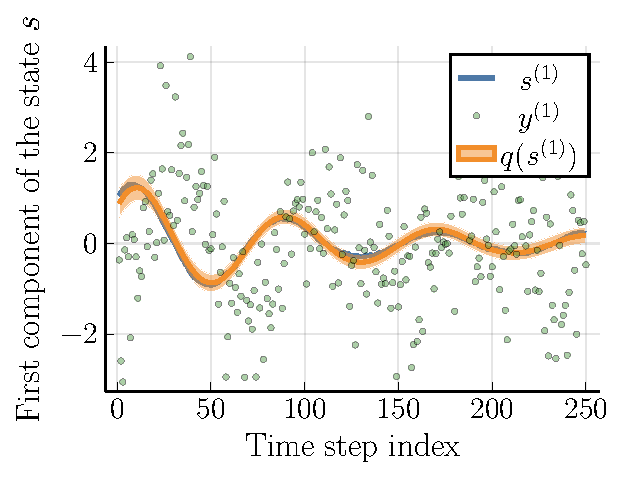
\includegraphics{contents/05-experiments/plots/lds/02-rotating_example_inference_states_1.pdf}
    }
    \caption{Simulated evolution of the first component of the state $s_t$ and its corresponding inferred posterior distribution.}
    \label{fig:sim:rotating_example_inference_states_1}
  \end{subfigure}
  \hfill
  \begin{subfigure}[t]{0.475\textwidth}
    \centering
    \resizebox{\textwidth}{!}{
        % % Recommended preamble:
% \usetikzlibrary{arrows.meta}
% \usetikzlibrary{backgrounds}
% \usepgfplotslibrary{patchplots}
% \usepgfplotslibrary{fillbetween}
% \pgfplotsset{%
%     layers/standard/.define layer set={%
%         background,axis background,axis grid,axis ticks,axis lines,axis tick labels,pre main,main,axis descriptions,axis foreground%
%     }{
%         grid style={/pgfplots/on layer=axis grid},%
%         tick style={/pgfplots/on layer=axis ticks},%
%         axis line style={/pgfplots/on layer=axis lines},%
%         label style={/pgfplots/on layer=axis descriptions},%
%         legend style={/pgfplots/on layer=axis descriptions},%
%         title style={/pgfplots/on layer=axis descriptions},%
%         colorbar style={/pgfplots/on layer=axis descriptions},%
%         ticklabel style={/pgfplots/on layer=axis tick labels},%
%         axis background@ style={/pgfplots/on layer=axis background},%
%         3d box foreground style={/pgfplots/on layer=axis foreground},%
%     },
% }

\begin{tikzpicture}[/tikz/background rectangle/.style={fill={rgb,1:red,1.0;green,1.0;blue,1.0}, fill opacity={1.0}, draw opacity={1.0}}, show background rectangle]
\begin{axis}[point meta max={nan}, point meta min={nan}, legend cell align={left}, legend columns={1}, title={}, title style={at={{(0.5,1)}}, anchor={south}, font={{\fontsize{18 pt}{23.400000000000002 pt}\selectfont}}, color={rgb,1:red,0.0;green,0.0;blue,0.0}, draw opacity={1.0}, rotate={0.0}, align={center}}, legend style={color={rgb,1:red,0.0;green,0.0;blue,0.0}, draw opacity={1.0}, line width={1}, solid, fill={rgb,1:red,1.0;green,1.0;blue,1.0}, fill opacity={1.0}, text opacity={1.0}, font={{\fontsize{14 pt}{18.2 pt}\selectfont}}, text={rgb,1:red,0.0;green,0.0;blue,0.0}, cells={anchor={center}}, at={(0.98, 0.98)}, anchor={north east}}, axis background/.style={fill={rgb,1:red,1.0;green,1.0;blue,1.0}, opacity={1.0}}, anchor={north west}, xshift={1.0mm}, yshift={-1.0mm}, width={99.6mm}, height={74.2mm}, scaled x ticks={false}, xlabel={Time step index}, x tick style={color={rgb,1:red,0.0;green,0.0;blue,0.0}, opacity={1.0}}, x tick label style={color={rgb,1:red,0.0;green,0.0;blue,0.0}, opacity={1.0}, rotate={0}}, xlabel style={at={(ticklabel cs:0.5)}, anchor=near ticklabel, at={{(ticklabel cs:0.5)}}, anchor={near ticklabel}, font={{\fontsize{16 pt}{20.8 pt}\selectfont}}, color={rgb,1:red,0.0;green,0.0;blue,0.0}, draw opacity={1.0}, rotate={0.0}}, xmajorgrids={true}, xmin={-6.469999999999999}, xmax={257.47}, xticklabels={{$0$,$50$,$100$,$150$,$200$,$250$}}, xtick={{0.0,50.0,100.0,150.0,200.0,250.0}}, xtick align={inside}, xticklabel style={font={{\fontsize{14 pt}{18.2 pt}\selectfont}}, color={rgb,1:red,0.0;green,0.0;blue,0.0}, draw opacity={1.0}, rotate={0.0}}, x grid style={color={rgb,1:red,0.0;green,0.0;blue,0.0}, draw opacity={0.1}, line width={0.5}, solid}, axis x line*={left}, x axis line style={color={rgb,1:red,0.0;green,0.0;blue,0.0}, draw opacity={1.0}, line width={1}, solid}, scaled y ticks={false}, ylabel={Second component of the state $s$}, y tick style={color={rgb,1:red,0.0;green,0.0;blue,0.0}, opacity={1.0}}, y tick label style={color={rgb,1:red,0.0;green,0.0;blue,0.0}, opacity={1.0}, rotate={0}}, ylabel style={at={(ticklabel cs:0.5)}, anchor=near ticklabel, at={{(ticklabel cs:0.5)}}, anchor={near ticklabel}, font={{\fontsize{16 pt}{20.8 pt}\selectfont}}, color={rgb,1:red,0.0;green,0.0;blue,0.0}, draw opacity={1.0}, rotate={0.0}}, ymajorgrids={true}, ymin={-3.773440983138788}, ymax={3.9784772025868813}, yticklabels={{$-3$,$-2$,$-1$,$0$,$1$,$2$,$3$}}, ytick={{-3.0,-2.0,-1.0,0.0,1.0,2.0,3.0}}, ytick align={inside}, yticklabel style={font={{\fontsize{14 pt}{18.2 pt}\selectfont}}, color={rgb,1:red,0.0;green,0.0;blue,0.0}, draw opacity={1.0}, rotate={0.0}}, y grid style={color={rgb,1:red,0.0;green,0.0;blue,0.0}, draw opacity={0.1}, line width={0.5}, solid}, axis y line*={left}, y axis line style={color={rgb,1:red,0.0;green,0.0;blue,0.0}, draw opacity={1.0}, line width={1}, solid}, colorbar={false}]
    \addplot[color={rgb,1:red,0.8824;green,0.3412;blue,0.349}, name path={b277fcc4-0eb0-4e6b-aac0-78c6e1dbefbe}, draw opacity={1.0}, line width={2}, solid]
        table[row sep={\\}]
        {
            \\
            1.0  0.9139423264996561  \\
            2.0  0.826681727437719  \\
            3.0  0.7419593801583712  \\
            4.0  0.6395678936444418  \\
            5.0  0.5299299034684026  \\
            6.0  0.40758872952938746  \\
            7.0  0.3235250200132954  \\
            8.0  0.2094682448971536  \\
            9.0  0.10610412391768732  \\
            10.0  -0.003879334667540137  \\
            11.0  -0.11092025905953526  \\
            12.0  -0.20178841757688326  \\
            13.0  -0.29396920543807664  \\
            14.0  -0.36603269742051014  \\
            15.0  -0.44580935330837196  \\
            16.0  -0.5201882194671443  \\
            17.0  -0.5868089638290946  \\
            18.0  -0.6798130575525809  \\
            19.0  -0.733504663017128  \\
            20.0  -0.7850957500182586  \\
            21.0  -0.8343124473037915  \\
            22.0  -0.8929270588444692  \\
            23.0  -0.9305320740802544  \\
            24.0  -0.9828198162406432  \\
            25.0  -1.0007398905275426  \\
            26.0  -1.0189119846286163  \\
            27.0  -1.0402235900460959  \\
            28.0  -1.0610681242100486  \\
            29.0  -1.0718901674619523  \\
            30.0  -1.0728834486335088  \\
            31.0  -1.0608274565877778  \\
            32.0  -1.0380053658637372  \\
            33.0  -1.005066844086312  \\
            34.0  -0.9979462164720146  \\
            35.0  -0.9777157434434284  \\
            36.0  -0.9487928231555944  \\
            37.0  -0.9187367538624566  \\
            38.0  -0.8709764172956501  \\
            39.0  -0.8072523636429166  \\
            40.0  -0.7356988533074598  \\
            41.0  -0.6485395354576281  \\
            42.0  -0.5915739758357391  \\
            43.0  -0.5400651297279758  \\
            44.0  -0.47233229656425957  \\
            45.0  -0.41707688605137694  \\
            46.0  -0.3584722223948842  \\
            47.0  -0.2850328474229366  \\
            48.0  -0.21418437346945865  \\
            49.0  -0.1249360437541312  \\
            50.0  -0.06278737784193722  \\
            51.0  0.003902981478126781  \\
            52.0  0.07939561342095575  \\
            53.0  0.1503231344879653  \\
            54.0  0.23012447476060877  \\
            55.0  0.28829828800698803  \\
            56.0  0.3495409276659987  \\
            57.0  0.40880977308310473  \\
            58.0  0.46057659539662255  \\
            59.0  0.5092355373670427  \\
            60.0  0.5428700897890725  \\
            61.0  0.5674365519512619  \\
            62.0  0.5951309397324664  \\
            63.0  0.622635799882942  \\
            64.0  0.6392722111102564  \\
            65.0  0.6775934796732691  \\
            66.0  0.7154292547034586  \\
            67.0  0.7412716707810474  \\
            68.0  0.7359539727162364  \\
            69.0  0.7381273466544576  \\
            70.0  0.7372970186350419  \\
            71.0  0.7257381783901173  \\
            72.0  0.7085311280239531  \\
            73.0  0.702673216653829  \\
            74.0  0.6815579560109366  \\
            75.0  0.6480522723071585  \\
            76.0  0.6222281020194852  \\
            77.0  0.5722725302089245  \\
            78.0  0.552792643775767  \\
            79.0  0.5134951129820832  \\
            80.0  0.4832046614643037  \\
            81.0  0.44132715145922635  \\
            82.0  0.40428374831331726  \\
            83.0  0.3703882293781391  \\
            84.0  0.32316273265678175  \\
            85.0  0.2826523685892491  \\
            86.0  0.2402038084909223  \\
            87.0  0.20280392745554593  \\
            88.0  0.13366514366150162  \\
            89.0  0.09413923492504898  \\
            90.0  0.07010523888345092  \\
            91.0  0.023187189576477134  \\
            92.0  -0.02145105280624087  \\
            93.0  -0.0541470238737735  \\
            94.0  -0.10242004788955544  \\
            95.0  -0.1140359209843899  \\
            96.0  -0.15116590713876357  \\
            97.0  -0.20123389999566954  \\
            98.0  -0.22288442538409894  \\
            99.0  -0.255758313316565  \\
            100.0  -0.2874200549798491  \\
            101.0  -0.31282121279654884  \\
            102.0  -0.355537579366091  \\
            103.0  -0.37762648664422294  \\
            104.0  -0.3814289173085238  \\
            105.0  -0.4000467648879884  \\
            106.0  -0.4148599534985854  \\
            107.0  -0.40660424013373125  \\
            108.0  -0.39560286044452553  \\
            109.0  -0.37280443203198405  \\
            110.0  -0.35906317064486015  \\
            111.0  -0.3480556694040281  \\
            112.0  -0.34606175675493966  \\
            113.0  -0.334364022157203  \\
            114.0  -0.3399788106828013  \\
            115.0  -0.318717335683333  \\
            116.0  -0.29743382854363126  \\
            117.0  -0.29060101355528095  \\
            118.0  -0.26342922636528876  \\
            119.0  -0.24836700078485785  \\
            120.0  -0.2119509619138454  \\
            121.0  -0.1920370626335401  \\
            122.0  -0.18929406145104422  \\
            123.0  -0.17557760492936383  \\
            124.0  -0.1590870982841247  \\
            125.0  -0.1265323383932624  \\
            126.0  -0.0955418474604389  \\
            127.0  -0.07370291461811844  \\
            128.0  -0.049931285420054386  \\
            129.0  -0.009245735704736132  \\
            130.0  0.01096168157990887  \\
            131.0  0.029290136909315607  \\
            132.0  0.04720586882236372  \\
            133.0  0.06093020967299039  \\
            134.0  0.08995159352810694  \\
            135.0  0.10249029810934993  \\
            136.0  0.1418410626748901  \\
            137.0  0.16430811285311836  \\
            138.0  0.17980366601649675  \\
            139.0  0.20143087139165564  \\
            140.0  0.216320035692829  \\
            141.0  0.20369283376698938  \\
            142.0  0.22794597921020943  \\
            143.0  0.24682348220551437  \\
            144.0  0.2479007338989781  \\
            145.0  0.2554791978042291  \\
            146.0  0.2747549628401238  \\
            147.0  0.28493122912108676  \\
            148.0  0.2840398500974614  \\
            149.0  0.28970038346906596  \\
            150.0  0.2874600193687455  \\
            151.0  0.2931207500692116  \\
            152.0  0.28805204121844513  \\
            153.0  0.26876120310786134  \\
            154.0  0.2543970762844578  \\
            155.0  0.2494208170197601  \\
            156.0  0.2181190249751138  \\
            157.0  0.2093718152694125  \\
            158.0  0.20571187879871172  \\
            159.0  0.20364792804152024  \\
            160.0  0.1863736075379721  \\
            161.0  0.17045637849378148  \\
            162.0  0.135357864822331  \\
            163.0  0.12251301141946089  \\
            164.0  0.11984690091373577  \\
            165.0  0.11401287998732441  \\
            166.0  0.10608274636502717  \\
            167.0  0.08789145526870515  \\
            168.0  0.07563647329121735  \\
            169.0  0.046575057769659825  \\
            170.0  0.03565477390828303  \\
            171.0  0.022851949588578536  \\
            172.0  -0.006711621847547845  \\
            173.0  -0.039111022686803706  \\
            174.0  -0.06016042564357352  \\
            175.0  -0.07884640276391389  \\
            176.0  -0.08884681550932189  \\
            177.0  -0.10350487189859674  \\
            178.0  -0.12633065422182393  \\
            179.0  -0.12563914616369193  \\
            180.0  -0.1432198491433109  \\
            181.0  -0.152971402697168  \\
            182.0  -0.1828578417667424  \\
            183.0  -0.2017916201801862  \\
            184.0  -0.2099466732525659  \\
            185.0  -0.2132710272646842  \\
            186.0  -0.2150271732292239  \\
            187.0  -0.21685644000546564  \\
            188.0  -0.2133107102699198  \\
            189.0  -0.23000489935578422  \\
            190.0  -0.2194748505056568  \\
            191.0  -0.20601570829912125  \\
            192.0  -0.1968392460503198  \\
            193.0  -0.19078248830590191  \\
            194.0  -0.1843855497769603  \\
            195.0  -0.17000030570050195  \\
            196.0  -0.1602922167976657  \\
            197.0  -0.1481081147004638  \\
            198.0  -0.14773064357856014  \\
            199.0  -0.12444957754403206  \\
            200.0  -0.11092464101369667  \\
            201.0  -0.10940526234819432  \\
            202.0  -0.09182205511641474  \\
            203.0  -0.07558432389908695  \\
            204.0  -0.0589516502884399  \\
            205.0  -0.05512455152423886  \\
            206.0  -0.029927278523380077  \\
            207.0  -0.011466900389324913  \\
            208.0  -0.017086654326913954  \\
            209.0  0.01726725326708235  \\
            210.0  0.03007559819449601  \\
            211.0  0.04103302120459719  \\
            212.0  0.05863171162044833  \\
            213.0  0.07066372534764255  \\
            214.0  0.07581430730487937  \\
            215.0  0.08503154175621909  \\
            216.0  0.07744923178761927  \\
            217.0  0.08627124401634062  \\
            218.0  0.10332036808987294  \\
            219.0  0.11040993164627995  \\
            220.0  0.11134366743440904  \\
            221.0  0.126565045103028  \\
            222.0  0.1522966937080266  \\
            223.0  0.1763887062076108  \\
            224.0  0.1937551519470064  \\
            225.0  0.19694801781599228  \\
            226.0  0.2127114265596669  \\
            227.0  0.22456037642771426  \\
            228.0  0.2308189415105174  \\
            229.0  0.24213662069648365  \\
            230.0  0.2408777828578093  \\
            231.0  0.2467884527170218  \\
            232.0  0.24929384951908454  \\
            233.0  0.25643884252022575  \\
            234.0  0.26499906618633423  \\
            235.0  0.263296603102505  \\
            236.0  0.23629103627802042  \\
            237.0  0.23971378709176214  \\
            238.0  0.23875079702685534  \\
            239.0  0.21799400063412455  \\
            240.0  0.22077211141311304  \\
            241.0  0.19597854627090522  \\
            242.0  0.17747164368310644  \\
            243.0  0.16112157125305193  \\
            244.0  0.14491247326445622  \\
            245.0  0.1409243394273801  \\
            246.0  0.13275765736740128  \\
            247.0  0.11598941184605666  \\
            248.0  0.0731015504445369  \\
            249.0  0.051352944405853716  \\
            250.0  0.027377421244445484  \\
        }
        ;
    \addlegendentry {$s^{(2)}$}
    \addplot[color={rgb,1:red,0.6902;green,0.4784;blue,0.6314}, name path={2a8b94b3-4860-4012-a612-94093116599d}, only marks, draw opacity={0.5}, line width={0}, solid, mark={*}, mark size={1.5 pt}, mark repeat={1}, mark options={color={rgb,1:red,0.0;green,0.0;blue,0.0}, draw opacity={0.5}, fill={rgb,1:red,0.6902;green,0.4784;blue,0.6314}, fill opacity={0.5}, line width={0.0}, rotate={0}, solid}]
        table[row sep={\\}]
        {
            \\
            1.0  2.6865034686904483  \\
            2.0  0.6610691815510777  \\
            3.0  2.3382434300604693  \\
            4.0  1.1863787582348655  \\
            5.0  0.7852739961894045  \\
            6.0  1.1165521934460583  \\
            7.0  0.6862219051102325  \\
            8.0  2.326206480620788  \\
            9.0  2.2774087281233646  \\
            10.0  3.759083291670117  \\
            11.0  0.24574643990836487  \\
            12.0  2.2390813868704207  \\
            13.0  1.7221941260314935  \\
            14.0  0.8783167116678238  \\
            15.0  1.4667798973723536  \\
            16.0  2.648559309391919  \\
            17.0  0.9162440389576378  \\
            18.0  1.286166430523954  \\
            19.0  2.481830944904276  \\
            20.0  0.26348404562393557  \\
            21.0  -0.49767581056023924  \\
            22.0  2.45841339706448  \\
            23.0  0.167830894573039  \\
            24.0  1.132639972935233  \\
            25.0  1.2598479286666127  \\
            26.0  0.6150026237167926  \\
            27.0  0.8580243460468271  \\
            28.0  -0.379441544541887  \\
            29.0  -1.1059305819906657  \\
            30.0  -0.7047780119408305  \\
            31.0  0.04072004145372124  \\
            32.0  0.5663572853759095  \\
            33.0  -1.271321080903285  \\
            34.0  -0.13406096165676754  \\
            35.0  0.27115200306861115  \\
            36.0  0.9608336288142406  \\
            37.0  -0.9185651959541206  \\
            38.0  -1.1519345745843226  \\
            39.0  -0.10084946262642958  \\
            40.0  -1.5198038857670202  \\
            41.0  -0.6553133307669605  \\
            42.0  -0.5859890702615758  \\
            43.0  -1.627087021090957  \\
            44.0  -1.4300669685060625  \\
            45.0  -0.17207990850707178  \\
            46.0  -0.7474842492339131  \\
            47.0  -2.380013250464666  \\
            48.0  -2.019032743724468  \\
            49.0  -2.4398153008351473  \\
            50.0  -0.6607066250222813  \\
            51.0  -2.376899124467764  \\
            52.0  -0.6851711207647544  \\
            53.0  -1.3480739281273344  \\
            54.0  -3.5540470722220237  \\
            55.0  -1.2983849588817857  \\
            56.0  -1.5244969131752595  \\
            57.0  -1.6735364636313514  \\
            58.0  -0.4835916978370802  \\
            59.0  -0.7031319954976907  \\
            60.0  -1.127304256396235  \\
            61.0  -1.2299229987585039  \\
            62.0  -1.0071616108756438  \\
            63.0  -1.2566003655814422  \\
            64.0  -0.9216579892703302  \\
            65.0  -0.3270484048098377  \\
            66.0  -0.11198876586159223  \\
            67.0  -0.26667387937713594  \\
            68.0  0.18134006187553064  \\
            69.0  0.326410656814323  \\
            70.0  0.4622953106848001  \\
            71.0  0.5328893872618697  \\
            72.0  0.5040861131207726  \\
            73.0  -0.2043928830264427  \\
            74.0  2.070110471425899  \\
            75.0  -1.0092224841422182  \\
            76.0  -0.09057123074773632  \\
            77.0  -0.2630778716623074  \\
            78.0  -0.46100623004134733  \\
            79.0  0.39783626289855023  \\
            80.0  2.2084477137456284  \\
            81.0  0.9906905182009027  \\
            82.0  -0.6137728823636632  \\
            83.0  1.1765946934799019  \\
            84.0  0.9431882273357916  \\
            85.0  -0.2034676501742606  \\
            86.0  0.8352127619283574  \\
            87.0  1.3374310336817794  \\
            88.0  1.8326201287181365  \\
            89.0  0.776640685804237  \\
            90.0  -1.9964739256137567  \\
            91.0  0.7459313455670961  \\
            92.0  -0.6822076206780749  \\
            93.0  -0.7376037792638788  \\
            94.0  0.8685030614269587  \\
            95.0  1.2360165776705268  \\
            96.0  -1.1874603496346179  \\
            97.0  1.9791418428326426  \\
            98.0  -1.0990999052892845  \\
            99.0  2.288573209597804  \\
            100.0  0.6506021112475333  \\
            101.0  1.3478384738069726  \\
            102.0  0.37398959442153695  \\
            103.0  -0.6699727562926593  \\
            104.0  -0.7977661721418449  \\
            105.0  0.657917871176291  \\
            106.0  0.389668128114737  \\
            107.0  0.24732874863436244  \\
            108.0  -1.4385617575829293  \\
            109.0  -0.2500398038255182  \\
            110.0  -0.07050976788558909  \\
            111.0  -0.21243543017334401  \\
            112.0  0.1417870033713586  \\
            113.0  -0.29708639963510586  \\
            114.0  0.41431040013233517  \\
            115.0  1.0615315761039532  \\
            116.0  0.08829362464490259  \\
            117.0  -0.5897428390687512  \\
            118.0  -1.3417129465148463  \\
            119.0  0.5081674123816606  \\
            120.0  -0.9080454760440475  \\
            121.0  -1.275598100717477  \\
            122.0  0.1919700514146484  \\
            123.0  -0.3732507412806464  \\
            124.0  -0.9181148134921402  \\
            125.0  -1.971573968908915  \\
            126.0  -0.5859254708840578  \\
            127.0  -0.6083964616231179  \\
            128.0  -1.072251663995012  \\
            129.0  -0.533917285526837  \\
            130.0  -0.10109156809324232  \\
            131.0  -0.889979952330008  \\
            132.0  -0.4589738962612315  \\
            133.0  -1.0463974329142296  \\
            134.0  -0.2125587378740768  \\
            135.0  -0.32098070549165636  \\
            136.0  0.25648396154227865  \\
            137.0  -1.2602171148134897  \\
            138.0  -1.3032216825921188  \\
            139.0  0.9621258771576597  \\
            140.0  -0.05066239867796257  \\
            141.0  0.030357168140001334  \\
            142.0  -0.409327474389966  \\
            143.0  -0.6184164905073706  \\
            144.0  -0.5623873446307848  \\
            145.0  -0.24092474139530617  \\
            146.0  1.0964630720225874  \\
            147.0  -0.7592186482097448  \\
            148.0  0.019561846218655227  \\
            149.0  -0.490510707908382  \\
            150.0  -1.72073899283562  \\
            151.0  0.4626674473075348  \\
            152.0  1.250924098010326  \\
            153.0  0.292769534174838  \\
            154.0  1.3909763579734946  \\
            155.0  -0.7273402316053436  \\
            156.0  -0.19014209211303892  \\
            157.0  -0.7400383371444402  \\
            158.0  -1.303394356172639  \\
            159.0  0.5014829789274512  \\
            160.0  0.18936153868567357  \\
            161.0  1.9689317447080905  \\
            162.0  -0.360530811400277  \\
            163.0  0.5036913740071914  \\
            164.0  -0.9535120939361754  \\
            165.0  -0.3208582214780097  \\
            166.0  2.4951593097229114  \\
            167.0  -0.5573712641245929  \\
            168.0  0.18847773548097235  \\
            169.0  1.8904728121295091  \\
            170.0  0.8961719879848076  \\
            171.0  -0.8276797089842443  \\
            172.0  1.2955435084017697  \\
            173.0  2.0197294560950194  \\
            174.0  -1.0664386421574785  \\
            175.0  0.6882393379542178  \\
            176.0  1.3233511874024162  \\
            177.0  2.093041228325718  \\
            178.0  -0.4134601183381302  \\
            179.0  1.5970697459736662  \\
            180.0  -1.3323770912809598  \\
            181.0  0.17557655410197526  \\
            182.0  2.051491310589964  \\
            183.0  -0.30018925076670744  \\
            184.0  1.4526956634985957  \\
            185.0  0.9146937684721315  \\
            186.0  0.03128593837357618  \\
            187.0  -0.13370535398757633  \\
            188.0  -1.1463800726627018  \\
            189.0  -1.2048652533209838  \\
            190.0  -1.015322207182953  \\
            191.0  -1.965722426801884  \\
            192.0  -1.1870466234504553  \\
            193.0  -0.4277646908539018  \\
            194.0  1.4052730581478545  \\
            195.0  0.009819201582386083  \\
            196.0  0.7839231291988403  \\
            197.0  -0.5914144140350177  \\
            198.0  1.5581572737883265  \\
            199.0  -0.2703232553011827  \\
            200.0  1.0770073738499093  \\
            201.0  0.5578735247288018  \\
            202.0  1.7807338428457837  \\
            203.0  2.037303951755668  \\
            204.0  -0.10936628936701313  \\
            205.0  -0.5456617375842041  \\
            206.0  -0.6886804483528325  \\
            207.0  -1.2571089843064878  \\
            208.0  -1.7215132690380863  \\
            209.0  0.08670140245278918  \\
            210.0  1.4444057998172384  \\
            211.0  1.0839005414250358  \\
            212.0  1.6707723049709937  \\
            213.0  -0.42697982959121916  \\
            214.0  -0.8986926171606712  \\
            215.0  0.7114299173358284  \\
            216.0  -1.214903761140543  \\
            217.0  -0.3551670645839455  \\
            218.0  -0.3425300449019031  \\
            219.0  1.9202065542984064  \\
            220.0  0.6317084761353249  \\
            221.0  -0.1851581506027628  \\
            222.0  0.8989311368910309  \\
            223.0  0.6554435951061048  \\
            224.0  0.49611402419480444  \\
            225.0  -1.3210707539195674  \\
            226.0  -0.7894098496276933  \\
            227.0  0.2840307972466564  \\
            228.0  0.7921099724793761  \\
            229.0  0.40049018859011326  \\
            230.0  0.6105042634695863  \\
            231.0  0.6188408843293506  \\
            232.0  -1.6029946287382706  \\
            233.0  -0.22616457883764707  \\
            234.0  0.7783643434606038  \\
            235.0  -0.7514975110596412  \\
            236.0  -0.5571857201195602  \\
            237.0  -0.5000718302584817  \\
            238.0  -1.0096728835221818  \\
            239.0  -0.5246807205812757  \\
            240.0  1.0392028208632964  \\
            241.0  -1.1964766315924071  \\
            242.0  1.1493149380044865  \\
            243.0  0.8520240640682426  \\
            244.0  2.0076560686852365  \\
            245.0  1.516683889749124  \\
            246.0  0.15629583096320263  \\
            247.0  1.7113785911244586  \\
            248.0  0.2635291735834718  \\
            249.0  0.7053764204846618  \\
            250.0  -0.4418834718210959  \\
        }
        ;
    \addlegendentry {$y^{(2)}$}
    \addplot+[line width={0}, draw opacity={0}, fill={rgb,1:red,0.4627;green,0.7176;blue,0.698}, fill opacity={0.5}, mark={none}, forget plot]
        coordinates {
            (1,1.019277409595826)
            (2,0.937920976332208)
            (3,0.8520507312894767)
            (4,0.7621681172781777)
            (5,0.669439115923124)
            (6,0.5745092877672441)
            (7,0.4778885540378565)
            (8,0.37981952625806953)
            (9,0.2813320289302292)
            (10,0.18300613565918686)
            (11,0.08536997946350212)
            (12,-0.011186744172810924)
            (13,-0.10601544839981059)
            (14,-0.19861033166842443)
            (15,-0.28818677930719433)
            (16,-0.374254642169673)
            (17,-0.45655103691375626)
            (18,-0.534593670576785)
            (19,-0.6077920152190482)
            (20,-0.6757648692241828)
            (21,-0.7385571753541718)
            (22,-0.7958615918642674)
            (23,-0.8472349671070474)
            (24,-0.8919347895402221)
            (25,-0.930250539589614)
            (26,-0.9623642121390357)
            (27,-0.987543999476449)
            (28,-1.006290457497983)
            (29,-1.0186317572317818)
            (30,-1.0244408748394023)
            (31,-1.0240556271632535)
            (32,-1.0170549114739609)
            (33,-1.0041028368040372)
            (34,-0.9851868831282168)
            (35,-0.9604095570507863)
            (36,-0.9299526902056722)
            (37,-0.8943518005843163)
            (38,-0.8537917545811153)
            (39,-0.8084607313280332)
            (40,-0.758329704658416)
            (41,-0.7045063057911225)
            (42,-0.6472755542943628)
            (43,-0.5869382959188648)
            (44,-0.5239575056569665)
            (45,-0.4587301055296177)
            (46,-0.3915782138369626)
            (47,-0.3229720208726418)
            (48,-0.2535955376003567)
            (49,-0.18364951628793177)
            (50,-0.11384505950187791)
            (51,-0.04459403084928743)
            (52,0.023757464240332562)
            (53,0.09114137176299784)
            (54,0.1569437679989614)
            (55,0.22039375999138539)
            (56,0.2812577552964301)
            (57,0.33931735068673263)
            (58,0.3944564021592386)
            (59,0.4456551611180235)
            (60,0.4928469324536207)
            (61,0.5360452041938829)
            (62,0.5749748724336367)
            (63,0.6096668745367365)
            (64,0.6398595237142635)
            (65,0.665340703637575)
            (66,0.6862040768495217)
            (67,0.7023212221776932)
            (68,0.7138740463167764)
            (69,0.7203542588585959)
            (70,0.72214596540079)
            (71,0.7192499185868778)
            (72,0.711850168592923)
            (73,0.6999841136233752)
            (74,0.6839707625109175)
            (75,0.6636376722797634)
            (76,0.6396764416711794)
            (77,0.612095614157788)
            (78,0.5813893123802784)
            (79,0.5473028972319902)
            (80,0.5104172153018951)
            (81,0.4709573102403396)
            (82,0.4291683444557128)
            (83,0.38528026047583946)
            (84,0.33969278646308554)
            (85,0.2930270907172081)
            (86,0.24551660570468337)
            (87,0.19729426089475693)
            (88,0.1490013511691946)
            (89,0.10054753692949756)
            (90,0.05242968868271645)
            (91,0.005104859281574017)
            (92,-0.04103220490913474)
            (93,-0.08589008418774752)
            (94,-0.12940165452550095)
            (95,-0.17116441190843054)
            (96,-0.21092010045693885)
            (97,-0.2484682041087624)
            (98,-0.2836626367390919)
            (99,-0.3162403595643061)
            (100,-0.34613002238043955)
            (101,-0.37333771652820197)
            (102,-0.3979588088452192)
            (103,-0.41957971033232866)
            (104,-0.4383080231639134)
            (105,-0.4537082648068601)
            (106,-0.4660909412432485)
            (107,-0.4753540146963264)
            (108,-0.48145159241225294)
            (109,-0.48462795666316105)
            (110,-0.48481050883719035)
            (111,-0.48220876767408793)
            (112,-0.47645513802984857)
            (113,-0.4679709313772932)
            (114,-0.45659535219219965)
            (115,-0.44255482739412455)
            (116,-0.4263496962946225)
            (117,-0.4078625774674309)
            (118,-0.38713038012507583)
            (119,-0.3646553342492902)
            (120,-0.3400716577375063)
            (121,-0.31395497804856554)
            (122,-0.28632853145610654)
            (123,-0.25727617028085026)
            (124,-0.2270160803832706)
            (125,-0.19618988737501034)
            (126,-0.1648318348519643)
            (127,-0.1331224372444316)
            (128,-0.10160069588107513)
            (129,-0.06968376694830661)
            (130,-0.03790125012832334)
            (131,-0.0065686789115227675)
            (132,0.02463180576209078)
            (133,0.055199030593025146)
            (134,0.08479024482831499)
            (135,0.11400812828694587)
            (136,0.14218240206221536)
            (137,0.16946520942985724)
            (138,0.19541668173399654)
            (139,0.21978995869600804)
            (140,0.2423438070390423)
            (141,0.2633257963018733)
            (142,0.2823988549550714)
            (143,0.2995111805930665)
            (144,0.31456771551625295)
            (145,0.3278157391746392)
            (146,0.33909500758474853)
            (147,0.3480769519655252)
            (148,0.35485253737460976)
            (149,0.35945542016660237)
            (150,0.36143931592119705)
            (151,0.3610969085422634)
            (152,0.35854418841236024)
            (153,0.3539435332259799)
            (154,0.34751398380655396)
            (155,0.33910997267205445)
            (156,0.3289103088726772)
            (157,0.31698067159895543)
            (158,0.3029266574067059)
            (159,0.28692256859011184)
            (160,0.2694826826883632)
            (161,0.25033171956185674)
            (162,0.2297105697377662)
            (163,0.2082031368605485)
            (164,0.18546510092179974)
            (165,0.16215029963453195)
            (166,0.13836881670551612)
            (167,0.11407262634910188)
            (168,0.0894020280956559)
            (169,0.06455132190912909)
            (170,0.03952847509790377)
            (171,0.014649993313948968)
            (172,-0.009888628894965676)
            (173,-0.03392204935534704)
            (174,-0.057357005369115185)
            (175,-0.08004201787634739)
            (176,-0.10187813241520577)
            (177,-0.12273585076091663)
            (178,-0.14252123869344685)
            (179,-0.1609700368007038)
            (180,-0.17781288194175165)
            (181,-0.1935559487982603)
            (182,-0.2075274198981314)
            (183,-0.21970613932648694)
            (184,-0.23012816416501977)
            (185,-0.23882671110708964)
            (186,-0.24569538215721215)
            (187,-0.25051507086622465)
            (188,-0.2533809769167398)
            (189,-0.25464897078108034)
            (190,-0.2543634868859117)
            (191,-0.2524382685959071)
            (192,-0.24930672287558156)
            (193,-0.2449968029772134)
            (194,-0.23954815089586143)
            (195,-0.23309104797005786)
            (196,-0.22536105291709996)
            (197,-0.21632600130765106)
            (198,-0.20630705643875769)
            (199,-0.19539897469331155)
            (200,-0.18379857790845516)
            (201,-0.17153663152587528)
            (202,-0.15835795556353574)
            (203,-0.14448903256155796)
            (204,-0.12941520029882686)
            (205,-0.11401607095942973)
            (206,-0.09795718975475415)
            (207,-0.08164298291125743)
            (208,-0.06541541326734181)
            (209,-0.0495193494618031)
            (210,-0.033677654811894775)
            (211,-0.01794240082444349)
            (212,-0.0022570028006499696)
            (213,0.013243375856030562)
            (214,0.028465074688689748)
            (215,0.04355308761608354)
            (216,0.05843945305515122)
            (217,0.07289311105617938)
            (218,0.08724119927569222)
            (219,0.10095604134212513)
            (220,0.11379454838575088)
            (221,0.12595996347599106)
            (222,0.13745471843096094)
            (223,0.14827653274109348)
            (224,0.15805137797239086)
            (225,0.16691131650639188)
            (226,0.17462999131652676)
            (227,0.18122534117365338)
            (228,0.18706547126683556)
            (229,0.19148594628421078)
            (230,0.19495736271052289)
            (231,0.19688773982964214)
            (232,0.19784084968153975)
            (233,0.19746147443691733)
            (234,0.19567592600898553)
            (235,0.19234278963663828)
            (236,0.18825900279838492)
            (237,0.18314820450907768)
            (238,0.17669774532072766)
            (239,0.16897249501844083)
            (240,0.16005021927436694)
            (241,0.14978529541142213)
            (242,0.13851258129032062)
            (243,0.126720394642869)
            (244,0.11444094643255319)
            (245,0.10152871557314683)
            (246,0.08782958764924459)
            (247,0.07392841054508009)
            (248,0.05991823127055344)
            (249,0.0457709550517576)
            (250,0.03171424689279253)
            (250,-0.1472542500369393)
            (249,-0.13208458411453958)
            (248,-0.1168764987420381)
            (247,-0.10186174165682069)
            (246,-0.08701519637736252)
            (245,-0.07243178913470105)
            (244,-0.0586971785985962)
            (243,-0.04565704405650822)
            (242,-0.03316470913767122)
            (241,-0.021250362026363184)
            (240,-0.010399522325696464)
            (239,-0.0009435749784872105)
            (238,0.00726714328368297)
            (237,0.01415936301057033)
            (236,0.0196730508413569)
            (235,0.024125915619591237)
            (234,0.027799483383695034)
            (233,0.029901971887002055)
            (232,0.03057982978301721)
            (231,0.029911552458043167)
            (230,0.02825684186219915)
            (229,0.025056001368249425)
            (228,0.02090460615914283)
            (227,0.015335116256144005)
            (226,0.009014445207532834)
            (225,0.0015763651010943514)
            (224,-0.0069957913315441544)
            (223,-0.016474988714310218)
            (222,-0.026993175296461974)
            (221,-0.03817672922022858)
            (220,-0.05002424143322569)
            (219,-0.06253941457278417)
            (218,-0.07592708952259876)
            (217,-0.0899460259057982)
            (216,-0.10407056906030296)
            (215,-0.11862997554311533)
            (214,-0.133395329168228)
            (213,-0.14830077022612437)
            (212,-0.16349329289955983)
            (211,-0.17888108374133074)
            (210,-0.19433063017699997)
            (209,-0.2098999376322812)
            (208,-0.22553810028896853)
            (207,-0.24152314925853863)
            (206,-0.2576108310975944)
            (205,-0.27345951859309753)
            (204,-0.2886648481616342)
            (203,-0.30356107698757484)
            (202,-0.31726815310378864)
            (201,-0.3303000793413835)
            (200,-0.3424295204064673)
            (199,-0.3539106392538388)
            (198,-0.36471152026851617)
            (197,-0.3746340906678395)
            (196,-0.38358227520486166)
            (195,-0.3912335563965919)
            (194,-0.39761874080395176)
            (193,-0.40300093818607374)
            (192,-0.40724858984148027)
            (191,-0.4103208556441762)
            (190,-0.41218868531505315)
            (189,-0.41241769427354097)
            (188,-0.41109329542272427)
            (187,-0.4081703549633685)
            (186,-0.40329245383351087)
            (185,-0.39636399696689856)
            (184,-0.38760384721391866)
            (183,-0.37711830574215754)
            (182,-0.36487419752939393)
            (181,-0.35083563453842675)
            (180,-0.33502405557877757)
            (179,-0.31811165943743464)
            (178,-0.29959273433859146)
            (177,-0.27973717019804795)
            (176,-0.25880979894747824)
            (175,-0.23690515500532489)
            (174,-0.2141533468863544)
            (173,-0.19065393269724443)
            (172,-0.1665589729297773)
            (171,-0.14196227536454586)
            (170,-0.11702967841000275)
            (169,-0.0919571132941172)
            (168,-0.0670614539805954)
            (167,-0.04235096085766353)
            (166,-0.018020146840314527)
            (165,0.005790558668058804)
            (164,0.02912913570820419)
            (163,0.05188553818100386)
            (162,0.0734060468263445)
            (161,0.0940351768225299)
            (160,0.1131892907876284)
            (159,0.13062782856576885)
            (158,0.1466264565803585)
            (157,0.16067133023633223)
            (156,0.17258861670137274)
            (155,0.18277321454054596)
            (154,0.19115995395118884)
            (153,0.19757053780379805)
            (152,0.20215103615659683)
            (151,0.20468288960324052)
            (150,0.2050041691666108)
            (149,0.20299928942988005)
            (148,0.1983759173553573)
            (147,0.19158062469876222)
            (146,0.18257997060173278)
            (145,0.17128312667322595)
            (144,0.15801871403821027)
            (143,0.14294694086472798)
            (142,0.1258204016813671)
            (141,0.10673393780762619)
            (140,0.08573904672143559)
            (139,0.06317241028496356)
            (138,0.03878599035033514)
            (137,0.012820480382949306)
            (136,-0.014477860761238887)
            (135,-0.04266981614907975)
            (134,-0.07190821821974297)
            (133,-0.10152350047316272)
            (132,-0.13211906308789423)
            (131,-0.16335286751798592)
            (130,-0.1947244279037283)
            (129,-0.22655224918450567)
            (128,-0.25852138556865945)
            (127,-0.29010275081277226)
            (126,-0.32187961275140436)
            (125,-0.3533132908112511)
            (124,-0.3842234759058464)
            (123,-0.4145760043172395)
            (122,-0.4437291972640999)
            (121,-0.47146467792437724)
            (120,-0.49769826365665787)
            (119,-0.5224062504206953)
            (118,-0.5450124111934185)
            (117,-0.565881806290587)
            (116,-0.5845113753358996)
            (115,-0.6008632877870911)
            (114,-0.6150539344425402)
            (113,-0.6265819414463853)
            (112,-0.6352198321861563)
            (111,-0.6411273689926835)
            (110,-0.6438822575721435)
            (109,-0.6438511959167206)
            (108,-0.6408238895915317)
            (107,-0.6348723182043778)
            (106,-0.6257517707277089)
            (105,-0.6135079321245481)
            (104,-0.5982428800592308)
            (103,-0.5796464177202973)
            (102,-0.558154621586743)
            (101,-0.533660776733353)
            (100,-0.5065796536168321)
            (99,-0.4768173539143147)
            (98,-0.4443695264624416)
            (97,-0.40930950973337443)
            (96,-0.3719025474349914)
            (95,-0.33229710851824523)
            (94,-0.29069622444492516)
            (93,-0.2473607480761832)
            (92,-0.20269580637530182)
            (91,-0.1567711131823446)
            (90,-0.10968058346555587)
            (89,-0.061821301829298014)
            (88,-0.013652440026435536)
            (87,0.03432729275595281)
            (86,0.08220673582072496)
            (85,0.12934348650026517)
            (84,0.17560394875551477)
            (83,0.22075450659446347)
            (82,0.26417432463314783)
            (81,0.30546454738016804)
            (80,0.3443966562272371)
            (79,0.3807274618227927)
            (78,0.414234425231901)
            (77,0.44433970175463056)
            (76,0.47130137669106414)
            (75,0.49462914569515926)
            (74,0.5143185638209726)
            (73,0.5296823000313949)
            (72,0.5408971054175084)
            (71,0.5476481758002532)
            (70,0.5499020589940452)
            (69,0.5474782307135242)
            (68,0.5403788822743201)
            (67,0.5282221147660523)
            (66,0.5115175462869925)
            (65,0.4900835977830359)
            (64,0.46404792408366413)
            (63,0.43331494083068545)
            (62,0.39809366179693145)
            (61,0.358641503351096)
            (60,0.3149221408065463)
            (59,0.2672042609127626)
            (58,0.21546704817759116)
            (57,0.15976910698225905)
            (56,0.1011215007702583)
            (55,0.03963127861000043)
            (54,-0.024492466310608224)
            (53,-0.09102546711034819)
            (52,-0.15920597164084563)
            (51,-0.22842881440648702)
            (50,-0.29863412374156895)
            (49,-0.36948321305858534)
            (48,-0.44057069268093507)
            (47,-0.5111908140414629)
            (46,-0.5811468906350514)
            (45,-0.6497575283302744)
            (44,-0.7165535536003804)
            (43,-0.7812121267125427)
            (42,-0.8433337461948798)
            (41,-0.9024509055270451)
            (40,-0.9582562166971166)
            (39,-1.0104560955338648)
            (38,-1.057932372416046)
            (37,-1.1007016836066517)
            (36,-1.1385618173218595)
            (35,-1.171312536947018)
            (34,-1.1984020234399537)
            (33,-1.2196317197107291)
            (32,-1.234882564675762)
            (31,-1.2441513584832642)
            (30,-1.2467598080385776)
            (29,-1.243117067542799)
            (28,-1.2328762609607498)
            (27,-1.2161588047977274)
            (26,-1.1929348026532458)
            (25,-1.1627061210250564)
            (24,-1.1262112207357835)
            (23,-1.0832788878217037)
            (22,-1.033634274385619)
            (21,-0.9780379525488754)
            (20,-0.9169540270597951)
            (19,-0.8507130777561355)
            (18,-0.7792950450532256)
            (17,-0.7031070216015439)
            (16,-0.6227658271840752)
            (15,-0.538779888919287)
            (14,-0.4514375656892555)
            (13,-0.36125338071433516)
            (12,-0.2690348300677702)
            (11,-0.17530875302458238)
            (10,-0.08074260527118918)
            (9,0.014257532599217082)
            (8,0.10914994523711596)
            (7,0.20334411482151477)
            (6,0.2958032703236102)
            (5,0.3862817374556495)
            (4,0.47427082355098105)
            (3,0.5591309032060677)
            (2,0.6397070355094135)
            (1,0.7155142716751246)
            (1,1.019277409595826)
        }
        ;
    \addplot+[line width={0}, draw opacity={0}, fill={rgb,1:red,0.4627;green,0.7176;blue,0.698}, fill opacity={0.5}, mark={none}, forget plot]
        coordinates {
            (1,1.019277409595826)
            (2,0.937920976332208)
            (3,0.8520507312894767)
            (4,0.7621681172781777)
            (5,0.669439115923124)
            (6,0.5745092877672441)
            (7,0.4778885540378565)
            (8,0.37981952625806953)
            (9,0.2813320289302292)
            (10,0.18300613565918686)
            (11,0.08536997946350212)
            (12,-0.011186744172810924)
            (13,-0.10601544839981059)
            (14,-0.19861033166842443)
            (15,-0.28818677930719433)
            (16,-0.374254642169673)
            (17,-0.45655103691375626)
            (18,-0.534593670576785)
            (19,-0.6077920152190482)
            (20,-0.6757648692241828)
            (21,-0.7385571753541718)
            (22,-0.7958615918642674)
            (23,-0.8472349671070474)
            (24,-0.8919347895402221)
            (25,-0.930250539589614)
            (26,-0.9623642121390357)
            (27,-0.987543999476449)
            (28,-1.006290457497983)
            (29,-1.0186317572317818)
            (30,-1.0244408748394023)
            (31,-1.0240556271632535)
            (32,-1.0170549114739609)
            (33,-1.0041028368040372)
            (34,-0.9851868831282168)
            (35,-0.9604095570507863)
            (36,-0.9299526902056722)
            (37,-0.8943518005843163)
            (38,-0.8537917545811153)
            (39,-0.8084607313280332)
            (40,-0.758329704658416)
            (41,-0.7045063057911225)
            (42,-0.6472755542943628)
            (43,-0.5869382959188648)
            (44,-0.5239575056569665)
            (45,-0.4587301055296177)
            (46,-0.3915782138369626)
            (47,-0.3229720208726418)
            (48,-0.2535955376003567)
            (49,-0.18364951628793177)
            (50,-0.11384505950187791)
            (51,-0.04459403084928743)
            (52,0.023757464240332562)
            (53,0.09114137176299784)
            (54,0.1569437679989614)
            (55,0.22039375999138539)
            (56,0.2812577552964301)
            (57,0.33931735068673263)
            (58,0.3944564021592386)
            (59,0.4456551611180235)
            (60,0.4928469324536207)
            (61,0.5360452041938829)
            (62,0.5749748724336367)
            (63,0.6096668745367365)
            (64,0.6398595237142635)
            (65,0.665340703637575)
            (66,0.6862040768495217)
            (67,0.7023212221776932)
            (68,0.7138740463167764)
            (69,0.7203542588585959)
            (70,0.72214596540079)
            (71,0.7192499185868778)
            (72,0.711850168592923)
            (73,0.6999841136233752)
            (74,0.6839707625109175)
            (75,0.6636376722797634)
            (76,0.6396764416711794)
            (77,0.612095614157788)
            (78,0.5813893123802784)
            (79,0.5473028972319902)
            (80,0.5104172153018951)
            (81,0.4709573102403396)
            (82,0.4291683444557128)
            (83,0.38528026047583946)
            (84,0.33969278646308554)
            (85,0.2930270907172081)
            (86,0.24551660570468337)
            (87,0.19729426089475693)
            (88,0.1490013511691946)
            (89,0.10054753692949756)
            (90,0.05242968868271645)
            (91,0.005104859281574017)
            (92,-0.04103220490913474)
            (93,-0.08589008418774752)
            (94,-0.12940165452550095)
            (95,-0.17116441190843054)
            (96,-0.21092010045693885)
            (97,-0.2484682041087624)
            (98,-0.2836626367390919)
            (99,-0.3162403595643061)
            (100,-0.34613002238043955)
            (101,-0.37333771652820197)
            (102,-0.3979588088452192)
            (103,-0.41957971033232866)
            (104,-0.4383080231639134)
            (105,-0.4537082648068601)
            (106,-0.4660909412432485)
            (107,-0.4753540146963264)
            (108,-0.48145159241225294)
            (109,-0.48462795666316105)
            (110,-0.48481050883719035)
            (111,-0.48220876767408793)
            (112,-0.47645513802984857)
            (113,-0.4679709313772932)
            (114,-0.45659535219219965)
            (115,-0.44255482739412455)
            (116,-0.4263496962946225)
            (117,-0.4078625774674309)
            (118,-0.38713038012507583)
            (119,-0.3646553342492902)
            (120,-0.3400716577375063)
            (121,-0.31395497804856554)
            (122,-0.28632853145610654)
            (123,-0.25727617028085026)
            (124,-0.2270160803832706)
            (125,-0.19618988737501034)
            (126,-0.1648318348519643)
            (127,-0.1331224372444316)
            (128,-0.10160069588107513)
            (129,-0.06968376694830661)
            (130,-0.03790125012832334)
            (131,-0.0065686789115227675)
            (132,0.02463180576209078)
            (133,0.055199030593025146)
            (134,0.08479024482831499)
            (135,0.11400812828694587)
            (136,0.14218240206221536)
            (137,0.16946520942985724)
            (138,0.19541668173399654)
            (139,0.21978995869600804)
            (140,0.2423438070390423)
            (141,0.2633257963018733)
            (142,0.2823988549550714)
            (143,0.2995111805930665)
            (144,0.31456771551625295)
            (145,0.3278157391746392)
            (146,0.33909500758474853)
            (147,0.3480769519655252)
            (148,0.35485253737460976)
            (149,0.35945542016660237)
            (150,0.36143931592119705)
            (151,0.3610969085422634)
            (152,0.35854418841236024)
            (153,0.3539435332259799)
            (154,0.34751398380655396)
            (155,0.33910997267205445)
            (156,0.3289103088726772)
            (157,0.31698067159895543)
            (158,0.3029266574067059)
            (159,0.28692256859011184)
            (160,0.2694826826883632)
            (161,0.25033171956185674)
            (162,0.2297105697377662)
            (163,0.2082031368605485)
            (164,0.18546510092179974)
            (165,0.16215029963453195)
            (166,0.13836881670551612)
            (167,0.11407262634910188)
            (168,0.0894020280956559)
            (169,0.06455132190912909)
            (170,0.03952847509790377)
            (171,0.014649993313948968)
            (172,-0.009888628894965676)
            (173,-0.03392204935534704)
            (174,-0.057357005369115185)
            (175,-0.08004201787634739)
            (176,-0.10187813241520577)
            (177,-0.12273585076091663)
            (178,-0.14252123869344685)
            (179,-0.1609700368007038)
            (180,-0.17781288194175165)
            (181,-0.1935559487982603)
            (182,-0.2075274198981314)
            (183,-0.21970613932648694)
            (184,-0.23012816416501977)
            (185,-0.23882671110708964)
            (186,-0.24569538215721215)
            (187,-0.25051507086622465)
            (188,-0.2533809769167398)
            (189,-0.25464897078108034)
            (190,-0.2543634868859117)
            (191,-0.2524382685959071)
            (192,-0.24930672287558156)
            (193,-0.2449968029772134)
            (194,-0.23954815089586143)
            (195,-0.23309104797005786)
            (196,-0.22536105291709996)
            (197,-0.21632600130765106)
            (198,-0.20630705643875769)
            (199,-0.19539897469331155)
            (200,-0.18379857790845516)
            (201,-0.17153663152587528)
            (202,-0.15835795556353574)
            (203,-0.14448903256155796)
            (204,-0.12941520029882686)
            (205,-0.11401607095942973)
            (206,-0.09795718975475415)
            (207,-0.08164298291125743)
            (208,-0.06541541326734181)
            (209,-0.0495193494618031)
            (210,-0.033677654811894775)
            (211,-0.01794240082444349)
            (212,-0.0022570028006499696)
            (213,0.013243375856030562)
            (214,0.028465074688689748)
            (215,0.04355308761608354)
            (216,0.05843945305515122)
            (217,0.07289311105617938)
            (218,0.08724119927569222)
            (219,0.10095604134212513)
            (220,0.11379454838575088)
            (221,0.12595996347599106)
            (222,0.13745471843096094)
            (223,0.14827653274109348)
            (224,0.15805137797239086)
            (225,0.16691131650639188)
            (226,0.17462999131652676)
            (227,0.18122534117365338)
            (228,0.18706547126683556)
            (229,0.19148594628421078)
            (230,0.19495736271052289)
            (231,0.19688773982964214)
            (232,0.19784084968153975)
            (233,0.19746147443691733)
            (234,0.19567592600898553)
            (235,0.19234278963663828)
            (236,0.18825900279838492)
            (237,0.18314820450907768)
            (238,0.17669774532072766)
            (239,0.16897249501844083)
            (240,0.16005021927436694)
            (241,0.14978529541142213)
            (242,0.13851258129032062)
            (243,0.126720394642869)
            (244,0.11444094643255319)
            (245,0.10152871557314683)
            (246,0.08782958764924459)
            (247,0.07392841054508009)
            (248,0.05991823127055344)
            (249,0.0457709550517576)
            (250,0.03171424689279253)
            (250,0.21068274382252436)
            (249,0.22362649421805478)
            (248,0.236712961283145)
            (247,0.24971856274698087)
            (246,0.2626743716758517)
            (245,0.2754892202809947)
            (244,0.2875790714637026)
            (243,0.2990978333422462)
            (242,0.31018987171831247)
            (241,0.3208209528492074)
            (240,0.33049996087443034)
            (239,0.3388885650153689)
            (238,0.3461283473577723)
            (237,0.352137046007585)
            (236,0.35684495475541295)
            (235,0.3605596636536853)
            (234,0.36355236863427604)
            (233,0.3650209769868326)
            (232,0.3651018695800623)
            (231,0.3638639272012411)
            (230,0.36165788355884665)
            (229,0.35791589120017214)
            (228,0.35322633637452827)
            (227,0.3471155660911628)
            (226,0.34024553742552066)
            (225,0.33224626791168943)
            (224,0.32309854727632586)
            (223,0.31302805419649715)
            (222,0.3019026121583839)
            (221,0.2900966561722107)
            (220,0.27761333820472744)
            (219,0.26445149725703443)
            (218,0.2504094880739832)
            (217,0.23573224801815695)
            (216,0.2209494751706054)
            (215,0.2057361507752824)
            (214,0.1903254785456075)
            (213,0.17478752193818548)
            (212,0.15897928729825989)
            (211,0.14299628209244378)
            (210,0.12697532055321042)
            (209,0.110861238708675)
            (208,0.09470727375428493)
            (207,0.07823718343602376)
            (206,0.06169645158808612)
            (205,0.045427376674238074)
            (204,0.029834447563980432)
            (203,0.0145830118644589)
            (202,0.0005522419767171882)
            (201,-0.012773183710367036)
            (200,-0.025167635410443034)
            (199,-0.03688731013278429)
            (198,-0.047902592608999206)
            (197,-0.05801791194746267)
            (196,-0.06713983062933829)
            (195,-0.07494853954352382)
            (194,-0.08147756098777109)
            (193,-0.08699266776835307)
            (192,-0.09136485590968282)
            (191,-0.09455568154763802)
            (190,-0.09653828845677026)
            (189,-0.09688024728861971)
            (188,-0.09566865841075528)
            (187,-0.09285978676908077)
            (186,-0.08809831048091343)
            (185,-0.08128942524728072)
            (184,-0.07265248111612088)
            (183,-0.06229397291081634)
            (182,-0.05018064226686886)
            (181,-0.03627626305809384)
            (180,-0.02060170830472574)
            (179,-0.0038284141639729485)
            (178,0.01455025695169776)
            (177,0.034265468676214675)
            (176,0.055053534117066705)
            (175,0.07682111925263012)
            (174,0.09943933614812402)
            (173,0.12280983398655035)
            (172,0.14678171513984598)
            (171,0.17126226199244382)
            (170,0.1960866286058103)
            (169,0.22105975711237535)
            (168,0.2458655101719072)
            (167,0.2704962135558673)
            (166,0.2947577802513468)
            (165,0.3185100406010051)
            (164,0.3418010661353953)
            (163,0.3645207355400931)
            (162,0.38601509264918793)
            (161,0.40662826230118354)
            (160,0.42577607458909794)
            (159,0.44321730861445485)
            (158,0.45922685823305326)
            (157,0.47329001296157863)
            (156,0.4852320010439817)
            (155,0.49544673080356294)
            (154,0.5038680136619191)
            (153,0.5103165286481617)
            (152,0.5149373406681237)
            (151,0.5175109274812862)
            (150,0.5178744626757833)
            (149,0.5159115509033247)
            (148,0.5113291573938622)
            (147,0.5045732792322881)
            (146,0.49561004456776425)
            (145,0.4843483516760524)
            (144,0.47111671699429564)
            (143,0.45607542032140497)
            (142,0.4389773082287757)
            (141,0.4199176547961204)
            (140,0.39894856735664896)
            (139,0.3764075071070525)
            (138,0.35204737311765794)
            (137,0.32610993847676517)
            (136,0.2988426648856696)
            (135,0.2706860727229715)
            (134,0.24148870787637294)
            (133,0.211921561659213)
            (132,0.1813826746120758)
            (131,0.15021550969494038)
            (130,0.1189219276470816)
            (129,0.08718471528789246)
            (128,0.05531999380650916)
            (127,0.023857876323909066)
            (126,-0.00778405695252421)
            (125,-0.03906648393876955)
            (124,-0.0698086848606948)
            (123,-0.099976336244461)
            (122,-0.1289278656481132)
            (121,-0.15644527817275383)
            (120,-0.18244505181835474)
            (119,-0.2069044180778851)
            (118,-0.22924834905673322)
            (117,-0.24984334864427477)
            (116,-0.2681880172533454)
            (115,-0.284246367001158)
            (114,-0.2981367699418591)
            (113,-0.30935992130820106)
            (112,-0.31769044387354084)
            (111,-0.3232901663554924)
            (110,-0.32573876010223723)
            (109,-0.3254047174096015)
            (108,-0.3220792952329742)
            (107,-0.3158357111882749)
            (106,-0.30643011175878804)
            (105,-0.2939085974891721)
            (104,-0.27837316626859593)
            (103,-0.25951300294435997)
            (102,-0.23776299610369547)
            (101,-0.213014656323051)
            (100,-0.18568039114404702)
            (99,-0.1556633652142975)
            (98,-0.12295574701574224)
            (97,-0.08762689848415037)
            (96,-0.04993765347888632)
            (95,-0.010031715298615879)
            (94,0.03189291539392322)
            (93,0.07558057970068816)
            (92,0.12063139655703235)
            (91,0.1669808317454926)
            (90,0.21453996083098875)
            (89,0.2629163756882931)
            (88,0.3116551423648247)
            (87,0.36026122903356106)
            (86,0.40882647558864177)
            (85,0.45671069493415106)
            (84,0.5037816241706563)
            (83,0.5498060143572154)
            (82,0.5941623642782777)
            (81,0.6364500731005112)
            (80,0.6764377743765531)
            (79,0.7138783326411877)
            (78,0.7485441995286557)
            (77,0.7798515265609455)
            (76,0.8080515066512948)
            (75,0.8326461988643676)
            (74,0.8536229612008623)
            (73,0.8702859272153555)
            (72,0.8828032317683377)
            (71,0.8908516613735025)
            (70,0.8943898718075348)
            (69,0.8932302870036677)
            (68,0.8873692103592328)
            (67,0.8764203295893341)
            (66,0.8608906074120508)
            (65,0.8405978094921142)
            (64,0.8156711233448628)
            (63,0.7860188082427876)
            (62,0.7518560830703418)
            (61,0.7134489050366698)
            (60,0.6707717241006952)
            (59,0.6241060613232844)
            (58,0.5734457561408861)
            (57,0.5188655943912062)
            (56,0.4613940098226019)
            (55,0.40115624137277034)
            (54,0.33838000230853105)
            (53,0.27330821063634386)
            (52,0.20672090012151076)
            (51,0.13924075270791217)
            (50,0.07094400473781311)
            (49,0.002184180482721787)
            (48,-0.06662038251977831)
            (47,-0.13475322770382075)
            (46,-0.2020095370388738)
            (45,-0.2677026827289609)
            (44,-0.3313614577135526)
            (43,-0.39266446512518693)
            (42,-0.45121736239384586)
            (41,-0.5065617060551999)
            (40,-0.5584031926197154)
            (39,-0.6064653671222016)
            (38,-0.6496511367461846)
            (37,-0.6880019175619808)
            (36,-0.7213435630894849)
            (35,-0.7495065771545546)
            (34,-0.7719717428164798)
            (33,-0.7885739538973454)
            (32,-0.7992272582721598)
            (31,-0.8039598958432428)
            (30,-0.802121941640227)
            (29,-0.7941464469207646)
            (28,-0.7797046540352162)
            (27,-0.7589291941551706)
            (26,-0.7317936216248256)
            (25,-0.6977949581541716)
            (24,-0.6576583583446607)
            (23,-0.6111910463923911)
            (22,-0.5580889093429158)
            (21,-0.49907639815946814)
            (20,-0.43457571138857043)
            (19,-0.364870952681961)
            (18,-0.2898922961003444)
            (17,-0.2099950522259686)
            (16,-0.1257434571552708)
            (15,-0.03759366969510164)
            (14,0.05421690235240664)
            (13,0.149222483914714)
            (12,0.24666134172214835)
            (11,0.3460487119515866)
            (10,0.4467548765895629)
            (9,0.5484065252612413)
            (8,0.6504891072790231)
            (7,0.7524329932541982)
            (6,0.853215305210878)
            (5,0.9525964943905985)
            (4,1.0500654110053742)
            (3,1.1449705593728856)
            (2,1.2361349171550025)
            (1,1.3230405475165272)
            (1,1.019277409595826)
        }
        ;
    \addplot[color={rgb,1:red,0.4627;green,0.7176;blue,0.698}, name path={13a33f81-3a28-4d87-baf9-01fdac02cade}, legend image code/.code={{
    \draw[fill={rgb,1:red,0.4627;green,0.7176;blue,0.698}, fill opacity={0.5}] (0cm,-0.1cm) rectangle (0.6cm,0.1cm);
    }}, draw opacity={1.0}, line width={2}, solid]
        table[row sep={\\}]
        {
            \\
            1.0  1.019277409595826  \\
            2.0  0.937920976332208  \\
            3.0  0.8520507312894767  \\
            4.0  0.7621681172781777  \\
            5.0  0.669439115923124  \\
            6.0  0.5745092877672441  \\
            7.0  0.4778885540378565  \\
            8.0  0.37981952625806953  \\
            9.0  0.2813320289302292  \\
            10.0  0.18300613565918686  \\
            11.0  0.08536997946350212  \\
            12.0  -0.011186744172810924  \\
            13.0  -0.10601544839981059  \\
            14.0  -0.19861033166842443  \\
            15.0  -0.28818677930719433  \\
            16.0  -0.374254642169673  \\
            17.0  -0.45655103691375626  \\
            18.0  -0.534593670576785  \\
            19.0  -0.6077920152190482  \\
            20.0  -0.6757648692241828  \\
            21.0  -0.7385571753541718  \\
            22.0  -0.7958615918642674  \\
            23.0  -0.8472349671070474  \\
            24.0  -0.8919347895402221  \\
            25.0  -0.930250539589614  \\
            26.0  -0.9623642121390357  \\
            27.0  -0.987543999476449  \\
            28.0  -1.006290457497983  \\
            29.0  -1.0186317572317818  \\
            30.0  -1.0244408748394023  \\
            31.0  -1.0240556271632535  \\
            32.0  -1.0170549114739609  \\
            33.0  -1.0041028368040372  \\
            34.0  -0.9851868831282168  \\
            35.0  -0.9604095570507863  \\
            36.0  -0.9299526902056722  \\
            37.0  -0.8943518005843163  \\
            38.0  -0.8537917545811153  \\
            39.0  -0.8084607313280332  \\
            40.0  -0.758329704658416  \\
            41.0  -0.7045063057911225  \\
            42.0  -0.6472755542943628  \\
            43.0  -0.5869382959188648  \\
            44.0  -0.5239575056569665  \\
            45.0  -0.4587301055296177  \\
            46.0  -0.3915782138369626  \\
            47.0  -0.3229720208726418  \\
            48.0  -0.2535955376003567  \\
            49.0  -0.18364951628793177  \\
            50.0  -0.11384505950187791  \\
            51.0  -0.04459403084928743  \\
            52.0  0.023757464240332562  \\
            53.0  0.09114137176299784  \\
            54.0  0.1569437679989614  \\
            55.0  0.22039375999138539  \\
            56.0  0.2812577552964301  \\
            57.0  0.33931735068673263  \\
            58.0  0.3944564021592386  \\
            59.0  0.4456551611180235  \\
            60.0  0.4928469324536207  \\
            61.0  0.5360452041938829  \\
            62.0  0.5749748724336367  \\
            63.0  0.6096668745367365  \\
            64.0  0.6398595237142635  \\
            65.0  0.665340703637575  \\
            66.0  0.6862040768495217  \\
            67.0  0.7023212221776932  \\
            68.0  0.7138740463167764  \\
            69.0  0.7203542588585959  \\
            70.0  0.72214596540079  \\
            71.0  0.7192499185868778  \\
            72.0  0.711850168592923  \\
            73.0  0.6999841136233752  \\
            74.0  0.6839707625109175  \\
            75.0  0.6636376722797634  \\
            76.0  0.6396764416711794  \\
            77.0  0.612095614157788  \\
            78.0  0.5813893123802784  \\
            79.0  0.5473028972319902  \\
            80.0  0.5104172153018951  \\
            81.0  0.4709573102403396  \\
            82.0  0.4291683444557128  \\
            83.0  0.38528026047583946  \\
            84.0  0.33969278646308554  \\
            85.0  0.2930270907172081  \\
            86.0  0.24551660570468337  \\
            87.0  0.19729426089475693  \\
            88.0  0.1490013511691946  \\
            89.0  0.10054753692949756  \\
            90.0  0.05242968868271645  \\
            91.0  0.005104859281574017  \\
            92.0  -0.04103220490913474  \\
            93.0  -0.08589008418774752  \\
            94.0  -0.12940165452550095  \\
            95.0  -0.17116441190843054  \\
            96.0  -0.21092010045693885  \\
            97.0  -0.2484682041087624  \\
            98.0  -0.2836626367390919  \\
            99.0  -0.3162403595643061  \\
            100.0  -0.34613002238043955  \\
            101.0  -0.37333771652820197  \\
            102.0  -0.3979588088452192  \\
            103.0  -0.41957971033232866  \\
            104.0  -0.4383080231639134  \\
            105.0  -0.4537082648068601  \\
            106.0  -0.4660909412432485  \\
            107.0  -0.4753540146963264  \\
            108.0  -0.48145159241225294  \\
            109.0  -0.48462795666316105  \\
            110.0  -0.48481050883719035  \\
            111.0  -0.48220876767408793  \\
            112.0  -0.47645513802984857  \\
            113.0  -0.4679709313772932  \\
            114.0  -0.45659535219219965  \\
            115.0  -0.44255482739412455  \\
            116.0  -0.4263496962946225  \\
            117.0  -0.4078625774674309  \\
            118.0  -0.38713038012507583  \\
            119.0  -0.3646553342492902  \\
            120.0  -0.3400716577375063  \\
            121.0  -0.31395497804856554  \\
            122.0  -0.28632853145610654  \\
            123.0  -0.25727617028085026  \\
            124.0  -0.2270160803832706  \\
            125.0  -0.19618988737501034  \\
            126.0  -0.1648318348519643  \\
            127.0  -0.1331224372444316  \\
            128.0  -0.10160069588107513  \\
            129.0  -0.06968376694830661  \\
            130.0  -0.03790125012832334  \\
            131.0  -0.0065686789115227675  \\
            132.0  0.02463180576209078  \\
            133.0  0.055199030593025146  \\
            134.0  0.08479024482831499  \\
            135.0  0.11400812828694587  \\
            136.0  0.14218240206221536  \\
            137.0  0.16946520942985724  \\
            138.0  0.19541668173399654  \\
            139.0  0.21978995869600804  \\
            140.0  0.2423438070390423  \\
            141.0  0.2633257963018733  \\
            142.0  0.2823988549550714  \\
            143.0  0.2995111805930665  \\
            144.0  0.31456771551625295  \\
            145.0  0.3278157391746392  \\
            146.0  0.33909500758474853  \\
            147.0  0.3480769519655252  \\
            148.0  0.35485253737460976  \\
            149.0  0.35945542016660237  \\
            150.0  0.36143931592119705  \\
            151.0  0.3610969085422634  \\
            152.0  0.35854418841236024  \\
            153.0  0.3539435332259799  \\
            154.0  0.34751398380655396  \\
            155.0  0.33910997267205445  \\
            156.0  0.3289103088726772  \\
            157.0  0.31698067159895543  \\
            158.0  0.3029266574067059  \\
            159.0  0.28692256859011184  \\
            160.0  0.2694826826883632  \\
            161.0  0.25033171956185674  \\
            162.0  0.2297105697377662  \\
            163.0  0.2082031368605485  \\
            164.0  0.18546510092179974  \\
            165.0  0.16215029963453195  \\
            166.0  0.13836881670551612  \\
            167.0  0.11407262634910188  \\
            168.0  0.0894020280956559  \\
            169.0  0.06455132190912909  \\
            170.0  0.03952847509790377  \\
            171.0  0.014649993313948968  \\
            172.0  -0.009888628894965676  \\
            173.0  -0.03392204935534704  \\
            174.0  -0.057357005369115185  \\
            175.0  -0.08004201787634739  \\
            176.0  -0.10187813241520577  \\
            177.0  -0.12273585076091663  \\
            178.0  -0.14252123869344685  \\
            179.0  -0.1609700368007038  \\
            180.0  -0.17781288194175165  \\
            181.0  -0.1935559487982603  \\
            182.0  -0.2075274198981314  \\
            183.0  -0.21970613932648694  \\
            184.0  -0.23012816416501977  \\
            185.0  -0.23882671110708964  \\
            186.0  -0.24569538215721215  \\
            187.0  -0.25051507086622465  \\
            188.0  -0.2533809769167398  \\
            189.0  -0.25464897078108034  \\
            190.0  -0.2543634868859117  \\
            191.0  -0.2524382685959071  \\
            192.0  -0.24930672287558156  \\
            193.0  -0.2449968029772134  \\
            194.0  -0.23954815089586143  \\
            195.0  -0.23309104797005786  \\
            196.0  -0.22536105291709996  \\
            197.0  -0.21632600130765106  \\
            198.0  -0.20630705643875769  \\
            199.0  -0.19539897469331155  \\
            200.0  -0.18379857790845516  \\
            201.0  -0.17153663152587528  \\
            202.0  -0.15835795556353574  \\
            203.0  -0.14448903256155796  \\
            204.0  -0.12941520029882686  \\
            205.0  -0.11401607095942973  \\
            206.0  -0.09795718975475415  \\
            207.0  -0.08164298291125743  \\
            208.0  -0.06541541326734181  \\
            209.0  -0.0495193494618031  \\
            210.0  -0.033677654811894775  \\
            211.0  -0.01794240082444349  \\
            212.0  -0.0022570028006499696  \\
            213.0  0.013243375856030562  \\
            214.0  0.028465074688689748  \\
            215.0  0.04355308761608354  \\
            216.0  0.05843945305515122  \\
            217.0  0.07289311105617938  \\
            218.0  0.08724119927569222  \\
            219.0  0.10095604134212513  \\
            220.0  0.11379454838575088  \\
            221.0  0.12595996347599106  \\
            222.0  0.13745471843096094  \\
            223.0  0.14827653274109348  \\
            224.0  0.15805137797239086  \\
            225.0  0.16691131650639188  \\
            226.0  0.17462999131652676  \\
            227.0  0.18122534117365338  \\
            228.0  0.18706547126683556  \\
            229.0  0.19148594628421078  \\
            230.0  0.19495736271052289  \\
            231.0  0.19688773982964214  \\
            232.0  0.19784084968153975  \\
            233.0  0.19746147443691733  \\
            234.0  0.19567592600898553  \\
            235.0  0.19234278963663828  \\
            236.0  0.18825900279838492  \\
            237.0  0.18314820450907768  \\
            238.0  0.17669774532072766  \\
            239.0  0.16897249501844083  \\
            240.0  0.16005021927436694  \\
            241.0  0.14978529541142213  \\
            242.0  0.13851258129032062  \\
            243.0  0.126720394642869  \\
            244.0  0.11444094643255319  \\
            245.0  0.10152871557314683  \\
            246.0  0.08782958764924459  \\
            247.0  0.07392841054508009  \\
            248.0  0.05991823127055344  \\
            249.0  0.0457709550517576  \\
            250.0  0.03171424689279253  \\
        }
        ;
    \addlegendentry {$q(s^{(2)})$}
\end{axis}
\end{tikzpicture}

        \includegraphics{contents/05-experiments/plots/lds/02-rotating_example_inference_states_2.pdf}
    }
    \caption{Simulated evolution of the second component of the state $s_t$ and its corresponding inferred posterior distribution.}
    \label{fig:sim:rotating_example_inference_states_2}
  \end{subfigure}
  \caption{
    Simulated evolution of the \ac{lds}~\eqref{eq:sim:lds}-\eqref{eq:sim:lds-stochastic-gaussian} in discrete time steps with state transition matrix $A =
      \begin{pmatrix}
        \cos(\frac{\pi}{20}) & \frac{\sin(\frac{\pi}{20})}{2} \\ -\frac{\sin(\frac{\pi}{20})}{2} & \cos(\frac{\pi}{20})
      \end{pmatrix}
    $, observational matrix $B =
      \begin{pmatrix}
        0.0 & -1.9 \\ 1.3 & 0.0
      \end{pmatrix}
    $, and noise components $\Sigma =
      \begin{pmatrix}
        10^{-4} & 0 \\ 0 & 10^{-4}
      \end{pmatrix}
    $, $\Omega =
      \begin{pmatrix}
        1 & 0 \\ 0 & 1
      \end{pmatrix}
    $.
    The state vector $s_t$ represents the real state of the system, has two components $(s^{(1)},
      s^{(2)})_t$, and cannot be observed directly.
    The vector $y_t$ represents corresponding noisy measurement, has two components $(y^{(1)},
      y^{(2)})_t$, and is linked to the state $s_t$ with the matrix $B$.
    The figure shows only the first $250$ time steps.
    The shaded area shows three standard deviations of the inferred posteriors from
    Listing~\ref{lst:sim:rotating_inference}.
  }
  \label{fig:sim:rotating_example_inference_states}
\end{figure}

\subsection{Scalability and performance characteristics}

\begin{figure}
  \centering
  \resizebox{\textwidth}{!}{
    % % Recommended preamble:
% \usetikzlibrary{arrows.meta}
% \usetikzlibrary{backgrounds}
% \usepgfplotslibrary{patchplots}
% \usepgfplotslibrary{fillbetween}
% \pgfplotsset{%
%     layers/standard/.define layer set={%
%         background,axis background,axis grid,axis ticks,axis lines,axis tick labels,pre main,main,axis descriptions,axis foreground%
%     }{
%         grid style={/pgfplots/on layer=axis grid},%
%         tick style={/pgfplots/on layer=axis ticks},%
%         axis line style={/pgfplots/on layer=axis lines},%
%         label style={/pgfplots/on layer=axis descriptions},%
%         legend style={/pgfplots/on layer=axis descriptions},%
%         title style={/pgfplots/on layer=axis descriptions},%
%         colorbar style={/pgfplots/on layer=axis descriptions},%
%         ticklabel style={/pgfplots/on layer=axis tick labels},%
%         axis background@ style={/pgfplots/on layer=axis background},%
%         3d box foreground style={/pgfplots/on layer=axis foreground},%
%     },
% }

\begin{tikzpicture}[/tikz/background rectangle/.style={fill={rgb,1:red,1.0;green,1.0;blue,1.0}, fill opacity={1.0}, draw opacity={1.0}}, show background rectangle]
\begin{axis}[point meta max={nan}, point meta min={nan}, legend cell align={left}, legend columns={1}, title={}, title style={at={{(0.5,1)}}, anchor={south}, font={{\fontsize{18 pt}{23.400000000000002 pt}\selectfont}}, color={rgb,1:red,0.0;green,0.0;blue,0.0}, draw opacity={1.0}, rotate={0.0}, align={center}}, legend style={color={rgb,1:red,0.0;green,0.0;blue,0.0}, draw opacity={1.0}, line width={1}, solid, fill={rgb,1:red,1.0;green,1.0;blue,1.0}, fill opacity={1.0}, text opacity={1.0}, font={{\fontsize{14 pt}{18.2 pt}\selectfont}}, text={rgb,1:red,0.0;green,0.0;blue,0.0}, cells={anchor={west}}, at={(1.02, 0.5)}, anchor={west}}, axis background/.style={fill={rgb,1:red,1.0;green,1.0;blue,1.0}, opacity={1.0}}, anchor={north west}, xshift={1.0mm}, yshift={-1.0mm}, width={196.2mm}, height={99.6mm}, scaled x ticks={false}, xlabel={Number of observation (log-scale)}, x tick style={color={rgb,1:red,0.0;green,0.0;blue,0.0}, opacity={1.0}}, x tick label style={color={rgb,1:red,0.0;green,0.0;blue,0.0}, opacity={1.0}, rotate={0}}, xlabel style={at={(ticklabel cs:0.5)}, anchor=near ticklabel, at={{(ticklabel cs:0.5)}}, anchor={near ticklabel}, font={{\fontsize{16 pt}{20.8 pt}\selectfont}}, color={rgb,1:red,0.0;green,0.0;blue,0.0}, draw opacity={1.0}, rotate={0.0}}, xmode={log}, log basis x={10}, xmajorgrids={true}, xmin={7.585775750291836}, xmax={131825.67385564075}, xticklabels={{$10^1$,$10^2$,$10^3$,$10^4$,$10^5$}}, xtick={{10,100,1000,10000,100000}}, xtick align={inside}, xticklabel style={font={{\fontsize{14 pt}{18.2 pt}\selectfont}}, color={rgb,1:red,0.0;green,0.0;blue,0.0}, draw opacity={1.0}, rotate={0.0}}, x grid style={color={rgb,1:red,0.0;green,0.0;blue,0.0}, draw opacity={0.1}, line width={0.5}, solid}, axis x line*={left}, x axis line style={color={rgb,1:red,0.0;green,0.0;blue,0.0}, draw opacity={1.0}, line width={1}, solid}, scaled y ticks={false}, ylabel={Time (in ms, log-scale)}, y tick style={color={rgb,1:red,0.0;green,0.0;blue,0.0}, opacity={1.0}}, y tick label style={color={rgb,1:red,0.0;green,0.0;blue,0.0}, opacity={1.0}, rotate={0}}, ylabel style={at={(ticklabel cs:0.5)}, anchor=near ticklabel, at={{(ticklabel cs:0.5)}}, anchor={near ticklabel}, font={{\fontsize{16 pt}{20.8 pt}\selectfont}}, color={rgb,1:red,0.0;green,0.0;blue,0.0}, draw opacity={1.0}, rotate={0.0}}, ymode={log}, log basis y={10}, ymajorgrids={true}, ymin={0.1}, ymax={100000.0}, yticklabels={{$10^{-1}$,$10^{0}$,$10^{1}$,$10^{2}$,$10^{3}$,$10^{4}$,$10^5$}}, ytick={{0.1,1.0,10.0,100.0,1000.0,10000.0,100000.0}}, ytick align={inside}, yticklabel style={font={{\fontsize{14 pt}{18.2 pt}\selectfont}}, color={rgb,1:red,0.0;green,0.0;blue,0.0}, draw opacity={1.0}, rotate={0.0}}, y grid style={color={rgb,1:red,0.0;green,0.0;blue,0.0}, draw opacity={0.1}, line width={0.5}, solid}, axis y line*={left}, y axis line style={color={rgb,1:red,0.0;green,0.0;blue,0.0}, draw opacity={1.0}, line width={1}, solid}, colorbar={false}]
    \addplot[color={rgb,1:red,0.0;green,0.6056;blue,0.9787}, name path={6f7ca86f-5a2d-4158-aaee-3bf576638a38}, draw opacity={1.0}, line width={1}, solid, mark={triangle*}, mark size={3.0 pt}, mark repeat={1}, mark options={color={rgb,1:red,0.0;green,0.0;blue,0.0}, draw opacity={1.0}, fill={rgb,1:red,0.0;green,0.6056;blue,0.9787}, fill opacity={1.0}, line width={0.75}, rotate={0}, solid}]
        table[row sep={\\}]
        {
            \\
            10.0  0.2996  \\
            20.0  0.5831  \\
            30.0  0.8668  \\
            50.0  1.422  \\
            100.0  2.9006  \\
            200.0  5.6734  \\
            300.0  8.6623  \\
            500.0  14.8744  \\
            1000.0  32.0284  \\
            2000.0  68.7959  \\
            3000.0  109.7784  \\
            5000.0  197.8897  \\
            10000.0  387.6957  \\
            50000.0  2064.0563  \\
            100000.0  4225.6265  \\
        }
        ;
    \addlegendentry {Reactive MP}
    \addplot[color={rgb,1:red,0.8889;green,0.4356;blue,0.2781}, name path={889801e1-5382-432b-a73f-c4464c5b28cb}, draw opacity={1.0}, line width={1}, dashed, mark={triangle*}, mark size={3.0 pt}, mark repeat={1}, mark options={color={rgb,1:red,0.0;green,0.0;blue,0.0}, draw opacity={1.0}, fill={rgb,1:red,0.8889;green,0.4356;blue,0.2781}, fill opacity={1.0}, line width={0.75}, rotate={180}, solid}]
        table[row sep={\\}]
        {
            \\
            10.0  0.1524  \\
            20.0  0.3112  \\
            30.0  0.4688  \\
            50.0  0.7861  \\
            100.0  1.6077  \\
            200.0  3.2485  \\
        }
        ;
    \addlegendentry {Scheduled MP (inference)}
    \addplot[color={rgb,1:red,0.2422;green,0.6433;blue,0.3044}, name path={e99f3202-de9f-4483-bd72-4ed8691c08ae}, draw opacity={1.0}, line width={1}, dashed, mark={triangle*}, mark size={3.0 pt}, mark repeat={1}, mark options={color={rgb,1:red,0.0;green,0.0;blue,0.0}, draw opacity={1.0}, fill={rgb,1:red,0.2422;green,0.6433;blue,0.3044}, fill opacity={1.0}, line width={0.75}, rotate={270}, solid}]
        table[row sep={\\}]
        {
            \\
            10.0  2223.7242  \\
            20.0  4477.2798  \\
            30.0  6738.2145  \\
            50.0  11230.5153  \\
            100.0  22537.9049  \\
            200.0  45060.0061  \\
        }
        ;
    \addlegendentry {Scheduled MP (compilation)}
    \addplot[color={rgb,1:red,0.7644;green,0.4441;blue,0.8243}, name path={c68d4663-37e3-4cb5-9708-966de0501e12}, draw opacity={1.0}, line width={1}, dotted, mark={triangle*}, mark size={3.0 pt}, mark repeat={1}, mark options={color={rgb,1:red,0.0;green,0.0;blue,0.0}, draw opacity={1.0}, fill={rgb,1:red,0.7644;green,0.4441;blue,0.8243}, fill opacity={1.0}, line width={0.75}, rotate={90}, solid}]
        table[row sep={\\}]
        {
            \\
            10.0  110.75  \\
            20.0  275.6353  \\
            30.0  854.5532  \\
            50.0  3040.8894  \\
            100.0  10996.676  \\
            200.0  27437.6725  \\
        }
        ;
    \addlegendentry {NUTS (100)}
    \addplot[color={rgb,1:red,0.6755;green,0.5557;blue,0.0942}, name path={c002ede6-5a53-445f-8530-102fed6d531b}, draw opacity={1.0}, line width={1}, dotted, mark={diamond*}, mark size={3.0 pt}, mark repeat={1}, mark options={color={rgb,1:red,0.0;green,0.0;blue,0.0}, draw opacity={1.0}, fill={rgb,1:red,0.6755;green,0.5557;blue,0.0942}, fill opacity={1.0}, line width={0.75}, rotate={0}, solid}]
        table[row sep={\\}]
        {
            \\
            10.0  216.8421  \\
            20.0  483.0576  \\
            30.0  1506.1875  \\
            50.0  6159.411  \\
            100.0  24572.7457  \\
            200.0  27371.4809  \\
        }
        ;
    \addlegendentry {NUTS (200)}
\end{axis}
\end{tikzpicture}

    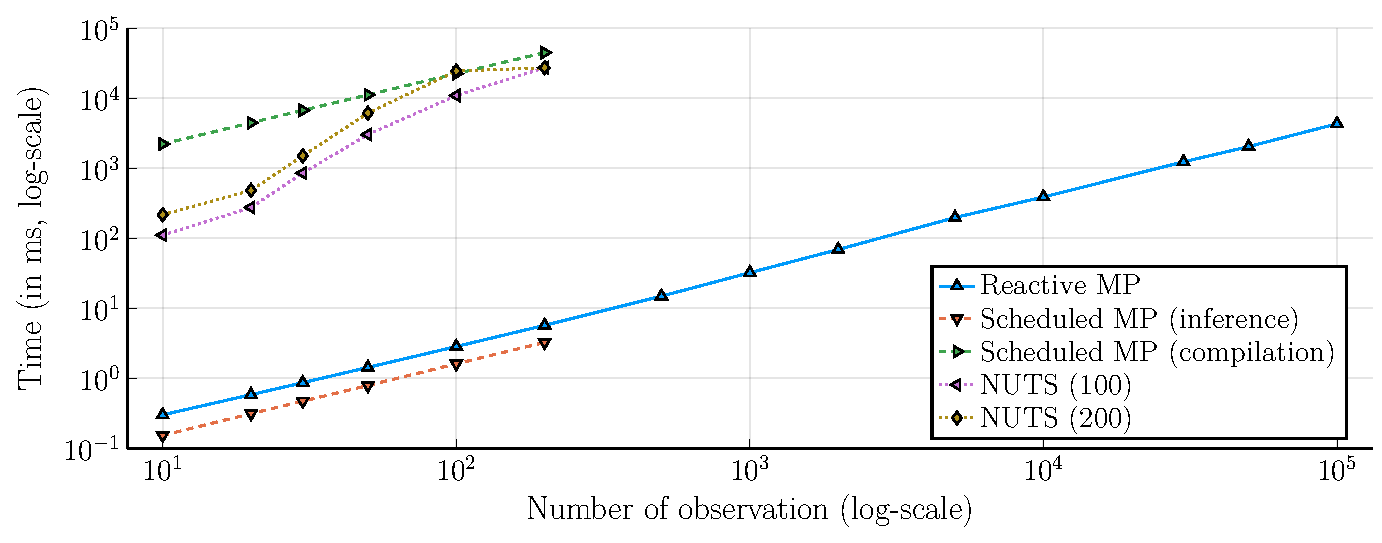
\includegraphics{contents/05-experiments/plots/lds/02-benchmark_comparison.pdf}
  }
  \caption{
    A comparison of run-time durations in milliseconds for automated Bayesian inference in the \ac{lds}~\eqref{eq:sim:lds}-\eqref{eq:sim:lds-stochastic-gaussian} with a 2-dimensional state is presented across
    different methods: reactive message passing (RxInfer), scheduled message passing (ForneyLab),
    and \ac{nuts} (Turing).
    The values in the table represent the minimum duration achieved across multiple runs.
    For RxInfer, the timings include the graph creation time.
    The ForneyLab pipeline involves model compilation followed by the execution of the inference
    procedure.
    Turing employs \ac{nuts} sampling with $100$ and $200$ samples, respectively.
    We provide benchmark results for over $300$ observations exclusively for the RxInfer
    framework.
  }
  \label{fig:sim:lds_performance_comparison}
\end{figure}

\begin{table}
  \centering
  \begin{tabular}{ |l||r|r|r|r|r|r|  }
    \hline
                    & \multicolumn{6}{|c|}{Number of observations}                                                                   \\
    \hline
                    & \multicolumn{3}{|c|}{2-dimensional}          & \multicolumn{3}{|c|}{4-dimensional}                             \\
    \hline
                    & 50                                           & 100                                 & 200  & 50   & 100  & 200  \\
    \hline
    Message passing & 2.80                                         & 2.78                                & 2.79 & 6.65 & 6.51 & 6.50 \\
    \hline
    NUTS (100)      & 2.85                                         & 2.78                                & 2.80 & 6.66 & 6.58 & 6.50 \\
    NUTS (200)      & 2.81                                         & 2.79                                & 2.80 & 6.65 & 6.52 & 6.50 \\
    \hline
  \end{tabular}
  \caption{
    Comparison of posterior result accuracy in terms of the metric~\eqref{eq:sim:average_mse} in the \ac{lds}~\eqref{eq:sim:lds}-\eqref{eq:sim:lds-stochastic-gaussian} among different methods: message passing (RxInfer and ForneyLab) and \ac{nuts} (Turing).
    Lower values indicate better performance.
    Both RxInfer and ForneyLab employ \ac{cbfe} minimization through \ac{vmp} on the full graph.
    Turing utilizes \ac{nuts} sampling with 100 and 200 samples, respectively.
  }
  \label{table:sim:lds_accuracy_comparison_2_4}
\end{table}

\begin{figure}
  \centering
  \begin{subfigure}[t]{\textwidth}
    \centering
    \resizebox{\textwidth}{!}{
        % % Recommended preamble:
% \usetikzlibrary{arrows.meta}
% \usetikzlibrary{backgrounds}
% \usepgfplotslibrary{patchplots}
% \usepgfplotslibrary{fillbetween}
% \pgfplotsset{%
%     layers/standard/.define layer set={%
%         background,axis background,axis grid,axis ticks,axis lines,axis tick labels,pre main,main,axis descriptions,axis foreground%
%     }{
%         grid style={/pgfplots/on layer=axis grid},%
%         tick style={/pgfplots/on layer=axis ticks},%
%         axis line style={/pgfplots/on layer=axis lines},%
%         label style={/pgfplots/on layer=axis descriptions},%
%         legend style={/pgfplots/on layer=axis descriptions},%
%         title style={/pgfplots/on layer=axis descriptions},%
%         colorbar style={/pgfplots/on layer=axis descriptions},%
%         ticklabel style={/pgfplots/on layer=axis tick labels},%
%         axis background@ style={/pgfplots/on layer=axis background},%
%         3d box foreground style={/pgfplots/on layer=axis foreground},%
%     },
% }

\begin{tikzpicture}[/tikz/background rectangle/.style={fill={rgb,1:red,1.0;green,1.0;blue,1.0}, fill opacity={1.0}, draw opacity={1.0}}, show background rectangle]
\begin{axis}[point meta max={nan}, point meta min={nan}, legend cell align={left}, legend columns={2}, title={}, title style={at={{(0.5,1)}}, anchor={south}, font={{\fontsize{18 pt}{23.400000000000002 pt}\selectfont}}, color={rgb,1:red,0.0;green,0.0;blue,0.0}, draw opacity={1.0}, rotate={0.0}, align={center}}, legend style={color={rgb,1:red,0.0;green,0.0;blue,0.0}, draw opacity={1.0}, line width={1}, solid, fill={rgb,1:red,1.0;green,1.0;blue,1.0}, fill opacity={1.0}, text opacity={1.0}, font={{\fontsize{14 pt}{18.2 pt}\selectfont}}, text={rgb,1:red,0.0;green,0.0;blue,0.0}, cells={anchor={west}}, at={(0.5, 1.02)}, anchor={south}}, axis background/.style={fill={rgb,1:red,1.0;green,1.0;blue,1.0}, opacity={1.0}}, anchor={north west}, xshift={1.0mm}, yshift={-1.0mm}, width={201.2mm}, height={74.2mm}, scaled x ticks={false}, xlabel={Number of observations in dataset (log10-scale)}, x tick style={color={rgb,1:red,0.0;green,0.0;blue,0.0}, opacity={1.0}}, x tick label style={color={rgb,1:red,0.0;green,0.0;blue,0.0}, opacity={1.0}, rotate={0}}, xlabel style={at={(ticklabel cs:0.5)}, anchor=near ticklabel, at={{(ticklabel cs:0.5)}}, anchor={near ticklabel}, font={{\fontsize{16 pt}{20.8 pt}\selectfont}}, color={rgb,1:red,0.0;green,0.0;blue,0.0}, draw opacity={1.0}, rotate={0.0}}, xmode={log}, log basis x={10}, xmajorgrids={true}, xmin={7.585775750291836}, xmax={131825.67385564075}, xticklabels={{$10^1$,$10^2$,$10^3$,$10^4$,$10^5$}}, xtick={{10,100,1000,10000,100000}}, xtick align={inside}, xticklabel style={font={{\fontsize{14 pt}{18.2 pt}\selectfont}}, color={rgb,1:red,0.0;green,0.0;blue,0.0}, draw opacity={1.0}, rotate={0.0}}, x grid style={color={rgb,1:red,0.0;green,0.0;blue,0.0}, draw opacity={0.1}, line width={0.5}, solid}, axis x line*={left}, x axis line style={color={rgb,1:red,0.0;green,0.0;blue,0.0}, draw opacity={1.0}, line width={1}, solid}, scaled y ticks={false}, ylabel={Time (in ms, log10-scale)}, y tick style={color={rgb,1:red,0.0;green,0.0;blue,0.0}, opacity={1.0}}, y tick label style={color={rgb,1:red,0.0;green,0.0;blue,0.0}, opacity={1.0}, rotate={0}}, ylabel style={at={(ticklabel cs:0.5)}, anchor=near ticklabel, at={{(ticklabel cs:0.5)}}, anchor={near ticklabel}, font={{\fontsize{16 pt}{20.8 pt}\selectfont}}, color={rgb,1:red,0.0;green,0.0;blue,0.0}, draw opacity={1.0}, rotate={0.0}}, ymode={log}, log basis y={10}, ymajorgrids={true}, ymin={0.1}, ymax={10000.0}, yticklabels={{$10^{-1}$,$10^{0}$,$10^{1}$,$10^{2}$,$10^{3}$,$10^{4}$}}, ytick={{0.1,1.0,10.0,100.0,1000.0,10000.0}}, ytick align={inside}, yticklabel style={font={{\fontsize{14 pt}{18.2 pt}\selectfont}}, color={rgb,1:red,0.0;green,0.0;blue,0.0}, draw opacity={1.0}, rotate={0.0}}, y grid style={color={rgb,1:red,0.0;green,0.0;blue,0.0}, draw opacity={0.1}, line width={0.5}, solid}, axis y line*={left}, y axis line style={color={rgb,1:red,0.0;green,0.0;blue,0.0}, draw opacity={1.0}, line width={1}, solid}, colorbar={false}]
    \addplot[color={rgb,1:red,0.3059;green,0.4745;blue,0.6549}, name path={e3a778d4-6418-4761-9fbc-ca4904cba719}, draw opacity={1.0}, line width={1}, solid, mark={diamond*}, mark size={3.0 pt}, mark repeat={1}, mark options={color={rgb,1:red,0.0;green,0.0;blue,0.0}, draw opacity={1.0}, fill={rgb,1:red,0.3059;green,0.4745;blue,0.6549}, fill opacity={1.0}, line width={0.75}, rotate={0}, solid}]
        table[row sep={\\}]
        {
            \\
            10.0  0.2931  \\
            20.0  0.5694  \\
            30.0  0.8533  \\
            50.0  1.4012  \\
            100.0  2.7853  \\
            200.0  5.6427  \\
            500.0  14.7833  \\
            1000.0  32.3217  \\
            2000.0  69.8363  \\
            5000.0  179.132  \\
            10000.0  377.7713  \\
            30000.0  1202.7147  \\
            50000.0  2038.2433  \\
            100000.0  4131.1598  \\
        }
        ;
    \addlegendentry {2 dimensional}
    \addplot[color={rgb,1:red,0.949;green,0.5569;blue,0.1686}, name path={e49bc6b2-00dd-4959-92f9-1db3bab8c102}, draw opacity={1.0}, line width={1}, dashed, mark={*}, mark size={3.0 pt}, mark repeat={1}, mark options={color={rgb,1:red,0.0;green,0.0;blue,0.0}, draw opacity={1.0}, fill={rgb,1:red,0.949;green,0.5569;blue,0.1686}, fill opacity={1.0}, line width={0.75}, rotate={0}, solid}]
        table[row sep={\\}]
        {
            \\
            10.0  0.2994  \\
            20.0  0.5814  \\
            30.0  0.8625  \\
            50.0  1.4243  \\
            100.0  2.8341  \\
            200.0  5.6979  \\
            500.0  14.8631  \\
            1000.0  32.2077  \\
            2000.0  69.0191  \\
            5000.0  197.8437  \\
            10000.0  388.9888  \\
            30000.0  1236.1908  \\
            50000.0  2044.8108  \\
            100000.0  4327.0868  \\
        }
        ;
    \addlegendentry {4 dimensional}
    \addplot[color={rgb,1:red,0.8824;green,0.3412;blue,0.349}, name path={d4bd6730-897d-4bb8-941f-c9226874147a}, draw opacity={1.0}, line width={1}, dotted, mark={square*}, mark size={3.0 pt}, mark repeat={1}, mark options={color={rgb,1:red,0.0;green,0.0;blue,0.0}, draw opacity={1.0}, fill={rgb,1:red,0.8824;green,0.3412;blue,0.349}, fill opacity={1.0}, line width={0.75}, rotate={0}, solid}]
        table[row sep={\\}]
        {
            \\
            10.0  0.3171  \\
            20.0  0.615  \\
            30.0  0.9157  \\
            50.0  1.5115  \\
            100.0  3.0052  \\
            200.0  6.0854  \\
            500.0  15.9601  \\
            1000.0  34.4974  \\
            2000.0  74.1862  \\
            5000.0  202.8761  \\
            10000.0  412.2831  \\
            30000.0  1327.4848  \\
            50000.0  2164.303  \\
            100000.0  4472.756  \\
        }
        ;
    \addlegendentry {8 dimensional}
    \addplot[color={rgb,1:red,0.4627;green,0.7176;blue,0.698}, name path={71e972a8-1a88-40e6-862d-a1d49a6be8c2}, draw opacity={1.0}, line width={1}, dashdotted, mark={triangle*}, mark size={3.0 pt}, mark repeat={1}, mark options={color={rgb,1:red,0.0;green,0.0;blue,0.0}, draw opacity={1.0}, fill={rgb,1:red,0.4627;green,0.7176;blue,0.698}, fill opacity={1.0}, line width={0.75}, rotate={0}, solid}]
        table[row sep={\\}]
        {
            \\
            10.0  0.4773  \\
            20.0  0.9561  \\
            30.0  1.4435  \\
            50.0  2.3992  \\
            100.0  4.7535  \\
            200.0  9.8103  \\
            500.0  25.7334  \\
            1000.0  53.8492  \\
            2000.0  111.9562  \\
            5000.0  300.5951  \\
            10000.0  579.3586  \\
            30000.0  1872.9722  \\
            50000.0  3063.1097  \\
            100000.0  6285.8989  \\
        }
        ;
    \addlegendentry {16 dimensional}
\end{axis}
\end{tikzpicture}

        \includegraphics{contents/05-experiments/plots/lds/02-rxinfer_rotating_scalability_size.pdf}
    }
    \caption{Scalability benchmark across different dimensionalities of the state vector with respect to the number of observations in the dataset.
    }
    \label{fig:sim:lds_scalability_size}
  \end{subfigure}
  \hfill
  \begin{subfigure}[t]{\textwidth}
    \centering
    \resizebox{\textwidth}{!}{
        % % Recommended preamble:
% \usetikzlibrary{arrows.meta}
% \usetikzlibrary{backgrounds}
% \usepgfplotslibrary{patchplots}
% \usepgfplotslibrary{fillbetween}
% \pgfplotsset{%
%     layers/standard/.define layer set={%
%         background,axis background,axis grid,axis ticks,axis lines,axis tick labels,pre main,main,axis descriptions,axis foreground%
%     }{
%         grid style={/pgfplots/on layer=axis grid},%
%         tick style={/pgfplots/on layer=axis ticks},%
%         axis line style={/pgfplots/on layer=axis lines},%
%         label style={/pgfplots/on layer=axis descriptions},%
%         legend style={/pgfplots/on layer=axis descriptions},%
%         title style={/pgfplots/on layer=axis descriptions},%
%         colorbar style={/pgfplots/on layer=axis descriptions},%
%         ticklabel style={/pgfplots/on layer=axis tick labels},%
%         axis background@ style={/pgfplots/on layer=axis background},%
%         3d box foreground style={/pgfplots/on layer=axis foreground},%
%     },
% }

\begin{tikzpicture}[/tikz/background rectangle/.style={fill={rgb,1:red,1.0;green,1.0;blue,1.0}, fill opacity={1.0}, draw opacity={1.0}}, show background rectangle]
\begin{axis}[point meta max={nan}, point meta min={nan}, legend cell align={left}, legend columns={1}, title={}, title style={at={{(0.5,1)}}, anchor={south}, font={{\fontsize{18 pt}{23.400000000000002 pt}\selectfont}}, color={rgb,1:red,0.0;green,0.0;blue,0.0}, draw opacity={1.0}, rotate={0.0}, align={center}}, legend style={color={rgb,1:red,0.0;green,0.0;blue,0.0}, draw opacity={1.0}, line width={1}, solid, fill={rgb,1:red,1.0;green,1.0;blue,1.0}, fill opacity={1.0}, text opacity={1.0}, font={{\fontsize{14 pt}{18.2 pt}\selectfont}}, text={rgb,1:red,0.0;green,0.0;blue,0.0}, cells={anchor={west}}, at={(1.02, 0.5)}, anchor={west}}, axis background/.style={fill={rgb,1:red,1.0;green,1.0;blue,1.0}, opacity={1.0}}, anchor={north west}, xshift={1.0mm}, yshift={-1.0mm}, width={196.2mm}, height={74.2mm}, scaled x ticks={false}, xlabel={Number of dimensions}, x tick style={color={rgb,1:red,0.0;green,0.0;blue,0.0}, opacity={1.0}}, x tick label style={color={rgb,1:red,0.0;green,0.0;blue,0.0}, opacity={1.0}, rotate={0}}, xlabel style={at={(ticklabel cs:0.5)}, anchor=near ticklabel, at={{(ticklabel cs:0.5)}}, anchor={near ticklabel}, font={{\fontsize{16 pt}{20.8 pt}\selectfont}}, color={rgb,1:red,0.0;green,0.0;blue,0.0}, draw opacity={1.0}, rotate={0.0}}, xmajorgrids={true}, xmin={1.58}, xmax={16.42}, xticklabels={{2,4,8,16}}, xtick={{2,4,8,16}}, xtick align={inside}, xticklabel style={font={{\fontsize{14 pt}{18.2 pt}\selectfont}}, color={rgb,1:red,0.0;green,0.0;blue,0.0}, draw opacity={1.0}, rotate={0.0}}, x grid style={color={rgb,1:red,0.0;green,0.0;blue,0.0}, draw opacity={0.1}, line width={0.5}, solid}, axis x line*={left}, x axis line style={color={rgb,1:red,0.0;green,0.0;blue,0.0}, draw opacity={1.0}, line width={1}, solid}, scaled y ticks={false}, ylabel={Time (in ms, log10-scale)}, y tick style={color={rgb,1:red,0.0;green,0.0;blue,0.0}, opacity={1.0}}, y tick label style={color={rgb,1:red,0.0;green,0.0;blue,0.0}, opacity={1.0}, rotate={0}}, ylabel style={at={(ticklabel cs:0.5)}, anchor=near ticklabel, at={{(ticklabel cs:0.5)}}, anchor={near ticklabel}, font={{\fontsize{16 pt}{20.8 pt}\selectfont}}, color={rgb,1:red,0.0;green,0.0;blue,0.0}, draw opacity={1.0}, rotate={0.0}}, ymode={log}, log basis y={10}, ymajorgrids={true}, ymin={0.1}, ymax={10000.0}, yticklabels={{$10^{-1}$,$10^{0}$,$10^{1}$,$10^{2}$,$10^{3}$,$10^{4}$}}, ytick={{0.1,1.0,10.0,100.0,1000.0,10000.0}}, ytick align={inside}, yticklabel style={font={{\fontsize{14 pt}{18.2 pt}\selectfont}}, color={rgb,1:red,0.0;green,0.0;blue,0.0}, draw opacity={1.0}, rotate={0.0}}, y grid style={color={rgb,1:red,0.0;green,0.0;blue,0.0}, draw opacity={0.1}, line width={0.5}, solid}, axis y line*={left}, y axis line style={color={rgb,1:red,0.0;green,0.0;blue,0.0}, draw opacity={1.0}, line width={1}, solid}, colorbar={false}]
    \addplot[color={rgb,1:red,0.3059;green,0.4745;blue,0.6549}, name path={a51e7468-e62c-4398-99ec-1b4cef59b1de}, draw opacity={1.0}, line width={1}, solid, mark={triangle*}, mark size={3.0 pt}, mark repeat={1}, mark options={color={rgb,1:red,0.0;green,0.0;blue,0.0}, draw opacity={1.0}, fill={rgb,1:red,0.3059;green,0.4745;blue,0.6549}, fill opacity={1.0}, line width={0.75}, rotate={0}, solid}]
        table[row sep={\\}]
        {
            \\
            2.0  0.2931  \\
            4.0  0.2994  \\
            8.0  0.3171  \\
            16.0  0.4773  \\
        }
        ;
    \addlegendentry {Reactive MP inference (10 observations)}
    \addplot[color={rgb,1:red,0.949;green,0.5569;blue,0.1686}, name path={ca5e1e4c-08d6-4d6a-9d55-9fb34d26d8ac}, draw opacity={1.0}, line width={1}, dashed, mark={triangle*}, mark size={3.0 pt}, mark repeat={1}, mark options={color={rgb,1:red,0.0;green,0.0;blue,0.0}, draw opacity={1.0}, fill={rgb,1:red,0.949;green,0.5569;blue,0.1686}, fill opacity={1.0}, line width={0.75}, rotate={180}, solid}]
        table[row sep={\\}]
        {
            \\
            2.0  32.3217  \\
            4.0  32.2077  \\
            8.0  34.4974  \\
            16.0  53.8492  \\
        }
        ;
    \addlegendentry {Reactive MP inference (1000 observations)}
    \addplot[color={rgb,1:red,0.8824;green,0.3412;blue,0.349}, name path={8c2f9457-3d7f-4552-bb01-ec5beeeb87ad}, draw opacity={1.0}, line width={1}, dotted, mark={triangle*}, mark size={3.0 pt}, mark repeat={1}, mark options={color={rgb,1:red,0.0;green,0.0;blue,0.0}, draw opacity={1.0}, fill={rgb,1:red,0.8824;green,0.3412;blue,0.349}, fill opacity={1.0}, line width={0.75}, rotate={270}, solid}]
        table[row sep={\\}]
        {
            \\
            2.0  377.7713  \\
            4.0  388.9888  \\
            8.0  412.2831  \\
            16.0  579.3586  \\
        }
        ;
    \addlegendentry {Reactive MP inference (10000 observations)}
    \addplot[color={rgb,1:red,0.4627;green,0.7176;blue,0.698}, name path={88323c08-2b3f-43b3-a41f-4b181db02a91}, draw opacity={1.0}, line width={1}, dashdotted, mark={triangle*}, mark size={3.0 pt}, mark repeat={1}, mark options={color={rgb,1:red,0.0;green,0.0;blue,0.0}, draw opacity={1.0}, fill={rgb,1:red,0.4627;green,0.7176;blue,0.698}, fill opacity={1.0}, line width={0.75}, rotate={90}, solid}]
        table[row sep={\\}]
        {
            \\
            2.0  4131.1598  \\
            4.0  4327.0868  \\
            8.0  4472.756  \\
            16.0  6285.8989  \\
        }
        ;
    \addlegendentry {Reactive MP inference (100000 observations)}
\end{axis}
\end{tikzpicture}

        \includegraphics{contents/05-experiments/plots/lds/02-rxinfer_rotating_scalability_dims.pdf}
    }
    \caption{Scalability benchmark across different numbers of observations in the dataset with respect to the dimensionality of the state vector.}
    \label{fig:sim:lds_scalability_dims}
  \end{subfigure}
  \hfill \caption{
    Benchmark results of automated Bayesian inference for the \ac{lds}~\eqref{eq:sim:lds}-\eqref{eq:sim:lds-stochastic-gaussian} using the RxInfer framework.
    The results illustrate the excellent scalability of the RxInfer framework for varying numbers
    of observations in the dataset and different dimensionalities of the state vector.
    The values in the table represent the minimum duration observed across multiple runs,
    including graph creation time.
  }
  \label{fig:sim:lds_scalability}
\end{figure}

This section demonstrates the scalability and run-time efficiency characteristics of the proposed \ac{rmp} architecture for the \ac{lds}~\eqref{eq:sim:lds}-\eqref{eq:sim:lds-stochastic-gaussian} compare to other methods.
The main benchmark results, which highlight the performance and scalability of the RxInfer
framework, are presented in Figure~\ref{fig:sim:lds_performance_comparison}.
The benchmark analysis reveals that the RxInfer framework achieves superior performance and
scalability compared to the alternative packages when considering both model creation and
inference execution.
It outperforms the packages compared in terms of time and memory consumption\footnote{Not
  present in the table.
}, indicating its
efficiency in handling the inference task \footnote{Detailed benchmark results,
  including comprehensive evaluations and comparisons of the RxInfer framework with ForneyLab
  and Turing across various experimental scenarios, can be found at
  \url{https://github.com/bvdmitri/phdthesis/tree/main/experiments}.
}.
Moreover, the RxInfer framework demonstrates its ability to handle large-scale models
consisting of hundreds of thousands of variables (\hyperlink{experiments:scalability}{\emph{Scalability}}).
This scalability is depicted in Figure~\ref{fig:sim:lds_scalability}, illustrating the
framework's ability to efficiently tackle complex Bayesian inference tasks involving
high-dimensional data.

Figure~\ref{fig:sim:lds_performance_comparison} reveals an interesting finding: the ForneyLab
package demonstrates faster execution of the inference task for this specific model compared
to the RxInfer framework.
This is attributed to ForneyLab's thorough analysis of the \ac{tffg} during precompilation,
enabling the creation of an efficient predefined message update schedule in advance.
As a result, the inference procedure is executed more efficiently.
However, it is important to note that ForneyLab's schedule-based approach suffers from
prolonged latencies in the graph creation and precompilation stages, as discussed in
Section~\ref{chapter-01:section:motivation}.
These stages experience high compilation times, and any modification in the model
specification requires complete recompilation.
This limitation restricts the exploration of "what-if" scenarios in the model specification
space and does not support online model structure adaptation, hindering the flexibility of the
scheduled message passing-based approaches.
In contrast, RxInfer adopts a dynamic approach by creating and executing the reactive message
passing scheme without relying on full graph analysis and naturally supports online model adaptation
in its core design.
This feature incurs certain run-time performance costs due to the additional management of reactive dependencies within the graph
during the inference process.
Despite these costs, RxInfer offers the advantage of adaptability and flexibility,
particularly when dealing with models of significant size and complexity.

The execution times of the \ac{nuts} algorithm, implemented in the Turing package, are mainly based
on the number of samples employed in the sampling procedure.
Generally, in sampling-based packages, a higher number of samples yields improved
approximations at the cost of longer computation times.
Determining an optimal number of samples is a nontrivial task, as it necessitates
consideration of the specific model and available dataset, as well as careful post-analysis of
the results.
For this experiment, the number of samples was manually selected to ensure that the
\ac{nuts} estimates of the corresponding posteriors exhibit precision comparable to the
message passing-based methods, as evaluated using the accuracy
metric~\eqref{eq:sim:average_mse}.
However, it should be noted that the sampling-based approach exhibits poor scalability when
confronted with a large number of latent states in a \ac{lds}, especially when the number of samples is large.
Consequently, its viability for real-time applications in the field is practically impossible.

We specifically focus on presenting benchmark results for a large number of observations using
the RxInfer framework, as executing the inference process with the alternative frameworks would
require significantly longer computation times, which are not suitable for real-time
applications.
To illustrate, Figure~\ref{fig:sim:lds_model_graph} provides an estimate that a static
dataset with $100,000$ observations results in a corresponding \ac{tffg}
for this model with approximately $700,000$ nodes.
RxInfer completes the inference task on a full model graph for such a size in less than ten
seconds, corresponding to less than $0.1$ milliseconds per observation (\hyperlink{experiments:efficiency}{\emph{Run-time efficiency and speed}}).
This result highlights the efficiency and scalability of the RxInfer framework.

In addition to performance and scalability, the accuracy of the estimated posteriors is a
critical factor in Bayesian inference.
Table~\ref{table:sim:lds_accuracy_comparison_2_4} presents the accuracy results in terms of
the \ac{ae} metric~\eqref{eq:sim:average_mse}.
It is observed that all methods yield comparable accuracy in estimating posteriors.
The scalability analysis for this type of model demonstrates that RxInfer can efficiently and
accurately perform inferences on this type of model (\hyperlink{experiments:accuracy}{\emph{Posterior accuracy}}).
This makes the \ac{rmp} framework, and RxInfer in particular, a better choice for real-world
applications involving high-dimensional data and linear dependencies among states.

In the subsequent section, we delve into running more difficult inference tasks in nonlinear
dynamical systems that share a similar structure to an \ac{lds} but entail more complex non-conjugate
relationships between variables.


\section{Non-linear dynamical system}\label{chapter-05:section:nonlinear-dynamical-system}

In this section, we delve into a more complex model and inference setting by considering a \ac{nlds}.
The real world is often "nonlinear" and many physical processes are better described by
nonlinear differential equations \citep{roubicek_nonlinear_2013}.
Inference in \acp{nlds} finds extensive applications in various industries beyond
signal processing \citep{Revach_kalmannet_2022}, including fields such as robotics
\citep{cernousko_control_2008}, astronomy \citep{Contopoulos_astronomy_nlds}, biology
\citep{Janson_bilogy_nlds}, economics \citep{hsieh_chaos_1991}, climate modeling
\citep{mukhin_principal_2015}, and many many more (\hyperlink{experiments:utility}{\emph{Utility}}).
As in the previous example, an \ac{nlds} is a state-space model that evolves over time
$t$, where the subsequent state of the system depends solely on the preceding state.
However, unlike the previous example, the relationship between subsequent states in this model is
nonlinear, introducing additional challenges in the inference process.

In its general form, an \ac{nlds} model can be expressed as follows
\begin{equation}
  \label{eq:sim:nlds}
  \begin{split}
    s_t &= f(s_{t - 1}) + v_{t}, \\% ~~\sigma_{t} \sim \mathcal{N}(0, \Sigma)\\ 
    y_t &= g(s_t) + w_{t}, % ~~\omega_{t} \sim \mathcal{N}(0, \Omega)
  \end{split}
\end{equation}
where $s_t$ denotes the state of the system at time $t$, and $f$
represents an arbitrary nonlinear state-transition function.
The observation at time $t$ is denoted by $y_t$, and $g$ represents an arbitrary (potentially
also nonlinear) observational function.
The terms $v_{t}$ and $w_{t}$ represent process and measurement noise signals and are often assumed to be Gaussian distributed with zero mean and
covariance matrices $\Sigma$ and $\Omega$, respectively:
\begin{equation}
    \label{eq:sim:nlds-stochastic-gaussian}
    \begin{split}
        v_{t} &\sim \mathcal{N}(0, \Sigma) \\
        w_{t} &\sim \mathcal{N}(0, \Omega) \\
    \end{split}
\end{equation}
By expressing the model~\eqref{eq:sim:nlds} with the assumption~\eqref{eq:sim:nlds-stochastic-gaussian} 
in terms of probability densities, we obtain the model specification
\begin{equation}
  \label{eq:sim:nlds_probabilities}
  \begin{aligned}
    p(s_t\vert s_{t-1}, \Sigma)
     & = \mathcal{N}(s_t \vert f(s_{t-1}), \Sigma) \\ p(y_t\vert s_{t}, \Omega) & = \mathcal{N}(y_t
       \vert g(s_{t}), \Omega)
  \end{aligned}
\end{equation}
where the first equation, $p(s_t\vert
  s_{t-1}, \Sigma)$, denotes the conditional probability distribution of the state $s_t$ given the
previous state $s_{t-1}$ and the covariance matrix $\Sigma$.
Similarly, the second equation, $p(y_t\vert s_{t}, \Omega)$, represents the conditional probability
distribution of the observation $y_t$ given the current state $s_t$ and the covariance
matrix $\Omega$.

The complete probabilistic model can be expressed as
\begin{equation}
  \label{eq:sim:nlds_model} p(\bm{y}, \bm{s}, \Sigma, \Omega) =
  \underbrace{p(\Sigma)p(\Omega)p(s_1)}_{\mathrm{prior}}\underbrace{\prod_{t = 1}^{T} p(y_t\vert
    s_t, \Omega)}_{\mathrm{likelihood}}\underbrace{\prod_{t = 2}^{T}p(s_t\vert s_{t - 1},
    \Sigma)}_{\mathrm{state~transitions}}
\end{equation}
where $p(\Sigma)$, $p(\Omega)$, and
$p(s_1)$ denote the priors for $\Sigma$, $\Omega$, and $s_1$, respectively.
Prior terms contribute to the overall prior probability of the model, incorporating prior
beliefs or knowledge about the covariance matrices and the initial state.
This formulation provides a comprehensive representation of the probabilistic model that
includes priors, likelihoods, and state transitions.
Figure~\eqref{fig:sim:lds_model_graph} provides a visual representation of the probabilistic
model~\eqref{eq:sim:lds_model} in the form of \ac{tffg}.
The \ac{tffg} visualizes the dependencies and flow of information within the model and illustrates
the interconnections between the different components of the \ac{nlds} model.

The probabilistic model~\eqref{eq:sim:nlds_model} is similar to the one discussed in
Section~\ref{chapter-05:section:linear-dynamical-system}, but with the notable difference that
both the transition and the observational functions are nonlinear.
The introduction of nonlinearities adds complexity to the inference procedure, as analytical
closed-form solutions for the exact Bayesian inference with arbitrary nonlinearities are generally not
available.
Therefore, we need to employ approximate inference techniques to estimate the posterior
distributions in this setting.

\begin{figure}
  \centering
  \resizebox{\textwidth}{!}{\begin{tikzpicture}
  \node[] (splink) {$\cdots$};
  \node[box, node distance=3mm] (spN) [right=of splink] {$\mathcal{N}$};
  \node[smallbox] (speq) [right=of spN] {\small $=$};
  \node[box, node distance=5mm] (spf) [right=of speq] {$f$};
  \node[box, node distance=5mm] (spfN) [right=of spf] {$\mathcal{N}$};
  \node[box, node distance=3mm] (spg) [below=of speq] {$g$};
  \node[box, node distance=3mm] (spgN) [below=of spg] {$\mathcal{N}$};
  \node[clamped, node distance=5mm] (yp) [below=of spgN] {};

  \path[line] (splink) edge[-] (spN);
  \path[line] (spN) edge[-] node[pos=0.5, anchor=south]{$s_{t - 1}$} (speq);
  \path[line] (speq) edge[-] (spf);
  \path[line] (speq) edge[-] (spg);
  \path[line] (spf) edge[-] (spfN);
  \path[line] (spg) edge[-] node[pos=0.5, anchor=east](spgleft){} node[pos=0.5, anchor=west](spgright){} (spgN);
  \path[line] (spgN) edge[-] node[pos=0.5, anchor=west]{$y_{t - 1}$} (yp);

  \node[smallbox] (seq) [right=of spfN] {\small $=$};
  \node[box, node distance=5mm] (sf) [right=of seq] {$f$};
  \node[box, node distance=5mm] (sfN) [right=of sf] {$\mathcal{N}$};
  \node[box, node distance=3mm] (sg) [below=of seq] {$g$};
  \node[box, node distance=3mm] (sgN) [below=of sg] {$\mathcal{N}$};
  \node[clamped, node distance=5mm] (y) [below=of sgN] {};

  \path[line] (spfN) edge[-] node[pos=0.5, anchor=south]{$s_{t}$} (seq);
  \path[line] (seq) edge[-] (sf);
  \path[line] (seq) edge[-] (sg);
  \path[line] (sf) edge[-] (sfN);
  \path[line] (sg) edge[-] node[pos=0.5, anchor=east](sgleft){} node[pos=0.5, anchor=west](sgright){} (sgN);
  \path[line] (sgN) edge[-] node[pos=0.5, anchor=west]{$y_{t}$} (y);

  \node[] (snlink) [right=of sfN] {$\cdots$};
  \node[box, node distance=5mm] (sTN) [right=of snlink] {$\mathcal{N}$};
  \node[smallbox, draw=white, node distance=5mm] (sTeq) [right=of sTN] {};
  \node[box, node distance=3mm] (sTg) [below=of sTeq] {$g$};
  \node[box, node distance=3mm] (sTgN) [below=of sTg] {$\mathcal{N}$};
  \node[clamped, node distance=5mm] (yT) [below=of sTgN] {};

  \path[line] (sfN) edge[-] node[pos=0.5, anchor=south]{$s_{t + 1}$} (snlink);
  \path[line] (snlink) edge[-] (sTN);
  \path[line] (sTN) edge[-] node[pos=0.5, anchor=south]{$s_T$} (sTeq.center);
  \draw[] (sTeq.center) -- (sTg);
  \path[line] (sTg) edge[-] node[pos=0.5, anchor=east](sTgleft){} node[pos=0.5, anchor=west](sTgright){} (sTgN);
  \path[line] (sTgN) edge[-] node[pos=0.5, anchor=west]{$y_{T}$} (yT);

  \node[box] (s0) [left=of splink] {$p(s_1)$};
  \path[line] (s0) edge[-] node[pos=0.5, anchor=south]{$s_1$} (splink);

  \node[smallbox] (pPsp) [above=of spN] {\small $=$};
  \node[node distance=4mm] (pPlink) [left=of pPsp] {$\cdots$};
  \node[box] (pP) [left=of pPlink] {$p(\Sigma)$};
  \node[smallbox] (pPs) [above=of spfN] {\small $=$};
  \node[smallbox] (pPsn) [above=of sfN] {\small $=$};
  \node[smallbox, draw=white] (pPsTeq) [right=of pPsn] {$\cdots$};

  \path[line] (pP) edge[-] node[pos=0.5, anchor=south]{$\Sigma$} (pPlink);
  \path[line] (pPlink) edge[-] (pPsp);
  \path[line] (pPsp) edge[-] (pPs);
  \path[line] (pPs) edge[-] (pPsn);
  \path[line] (pPsn) edge[-] (pPsTeq);
  \path[line] (pPsp) edge[-] (spN);
  \path[line] (pPs) edge[-] (spfN);
  \path[line] (pPsn) edge[-] (sfN);
  \draw[] (pPsTeq) -| (sTN);

  \node[smallbox] (pQsp) [left=of spgleft] {\small $=$};
  \node[smallbox] (pQs) [left=of sgleft] {\small $=$};
  \node[smallbox, draw=white, node distance=17mm] (pQsT) [left=of sTgleft] {$\cdots$};
  \node[] (pQsTextra) [right=of pQsT] {};
  \node[node distance=5mm] (pQlink) [left=of pQsp] {$\cdots$};
  \node[box] (pQ) [left=of pQlink] {$p(\Omega)$};

  \path[line] (pQ) edge[-] node[pos=0.5, anchor=south]{$\Omega$} (pQlink);
  \path[line] (pQlink) edge[-] (pQsp);
  \draw[] (pQsp) -- (spgleft.center);
  %\draw[path, densely dotted] (spgleft.center) -- (spgright.center);
  \draw[] (spgright.center) -- (pQs);
  \draw[] (pQs) -- (sgleft.center);
  %\draw[path, densely dotted] (sgleft.center) -- (sgright.center);
  \draw[] (sgright.center) -- (pQsT);
  \draw[] (pQsT) -- (pQsTextra.center);
  \draw[] (pQsTextra.center) |- (sTgN);
  \draw[] (pQsp) |- (spgN);
  \draw[] (pQs) |- (sgN);

\end{tikzpicture}

}
  \caption{
    A \ac{tffg} representation of the probabilistic model~\eqref{eq:sim:nlds_model} for the \ac{nlds}~\eqref{eq:sim:nlds}-\eqref{eq:sim:nlds-stochastic-gaussian}.
    The $s_t$ represent the hidden states, while $y_t$ corresponds to the
    observations.
    The $\Sigma$ and $\Omega$ are covariance matrices of the Gaussian noise components for states
    and observations, respectively.
    The state transition function $f$ and observational function $g$ are the nonlinear components of the model.
    Factor nodes $f$ and $g$ indicate a nonlinear function.
    The $\cdots$ symbol denotes the repetitive structure in the corresponding graph.
  }
  \label{fig:sim:nlds_model_graph}
\end{figure}

\subsection{Example of a nonlinear dynamical system}

As a particular simplistic example of an \ac{nlds} system, we choose the dynamics of a double
pendulum physical system.
The double pendulum system consists of two pendulums (rods) connected to each other.
Despite its simple appearance, the double pendulum exhibits complex and chaotic behavior,
making it an interesting case study \citep{levien_double_1993}.
Figure~\ref{fig:sim:double_pendulum_notation} provides an illustration of the double
pendulum system, depicting the rods and their movement restricted to two dimensions in the
vertical plane.
The dynamics of the double pendulum is described by a set of coupled ordinary differential
equations, which capture the relationship between the state of pendulums and their motion.
Due to its chaotic nature, the behavior of the double pendulum is highly sensitive to the
initial conditions, resulting in unpredictable and complex motion patterns.

% The motion equations of the double pendulum system can be discretized in time and solved
% numerically using methods such as the Runge-Kutta method
% \citep[Chapter~8]{hasselblatt_handbook_2002}.
Assuming that $s_t$ is the state of the system at time $t$, the evolution of the state of the double pendulum system can be
rewritten as \ac{nlds}~\eqref{eq:sim:nlds} (see Appendix~\ref{appendix:proofs:double_pendulum_dynamics}). 
Similar to the previous example in Section~\ref{chapter-05:section:linear-dynamical-system}, the number of latent states in the system increases linearly with the number of available observations.
The primary challenge lies in accurately estimating and tracking the evolution of the latent
states of the system given noisy measurements at specific points in time. 
More formally, we are interested in estimating the following Bayesian posteriors:
\begin{equation}
    \label{eq:sim:nlds-problem-statement}
    p(s_t\vert\hat{\bm{y}}_{1:T}) = \int p(\bm{y}, \bm{s}, \Sigma, \Omega)\prod_{i = 1}^{T}\delta(y_i - \hat{y}_i)\mathrm{d}\Sigma\mathrm{d}\Omega\mathrm{d}s_{\setminus t}\mathrm{d}\bm{y}~~\forall t \in 1:T.
\end{equation}

\begin{figure}
  \centering
  \resizebox{0.75\textwidth}{!}{\begin{tikzpicture}

  \node[fill=black, circle, inner sep=0.25mm, label={above left:{\tiny $(0, 0)$}}] (origin) {};
  \node[node distance=30mm] (xaxis) [right=of origin] {};
  \node[node distance=15mm] (yaxis) [below=of origin] {};

  \path[] ([xshift=-4mm]origin.center) edge[-stealth] node[pos=1.0, anchor=south]{\tiny $x$} (xaxis.center);
  \path[] ([yshift=4mm]origin.center) edge[stealth-] node[pos=0.0, anchor=south]{\tiny $y$} (yaxis.center);

  \node[circle, fill=black, inner sep=0.5mm, label={right:{\tiny $m_1$}}] (m1) [xshift=13mm, yshift=-6mm] {};
  \node[circle, fill=black, inner sep=0.5mm, label={right:{\tiny $m_2$}}] (m2) [xshift=20mm, yshift=-15mm] {};

  \path[-, densely dotted] ([xshift=13mm]origin.center) edge[-] node[pos=0, anchor=south]{\tiny $x_1$} (m1.center);
  \path[-, densely dotted] ([yshift=-6mm]origin.center) edge[-] node[pos=0, anchor=east]{\tiny $y_1$} (m1.center);
  \path[line] (origin) edge[-] node[pos=0.7, anchor=south]{\tiny $l_1$} (m1);

  \path[-, densely dotted] ([xshift=20mm]origin.center) edge[-] node[pos=0, anchor=south]{\tiny $x_2$} (m2.center);
  \path[-, densely dotted] ([yshift=-15mm]origin.center) edge[-] node[pos=0, anchor=east]{\tiny $y_2$} (m2.center);
  \path[line] (m1) edge[-] node[pos=0.7, anchor=south]{\tiny $l_2$} (m2);

  \node[node distance=5mm] (belowm1) [below=of m1] {};
  \path[-, densely dotted] (m1) edge[-] (belowm1);

  \pic [draw, -, radius=1mm] {angle = yaxis--origin--m1};
  \pic [draw, -, radius=1mm] {angle = belowm1--m1--m2};

  \node[] (t1) [xshift=5.0mm, yshift=-4.5mm]{\tiny $\theta_1$};
  \node[] (t1) [xshift=15.5mm, yshift=-12mm]{\tiny $\theta_2$};

  \node[] (gstart) [xshift=27.5mm, yshift=-3mm] {};
  \node[] (gend) [xshift=27.5mm, yshift=-10mm] {};
  \path[] (gstart) edge[-stealth] node[pos=0.5, anchor=west]{\tiny $g$} (gend);
\end{tikzpicture}
}
  \caption{
    An illustration of the double pendulum system.
    The system consists of two rods with lengths $l_i$ and two bobs with masses $m_i$.
    The rods are connected to each other.
    The state of the system at time $t$ is fully described by the state vector $(\theta_1,
      \theta_2, \dot{\theta}_1, \dot{\theta}_2)_t$, where $\theta_1$ and $\theta_2$ represent the 
      relative angles and $\dot{\theta}_1$ and $\dot{\theta}_2$ represent the angular velocities,
    respectively.
    The vector $g$ represents the gravitational force.
  }
  \label{fig:sim:double_pendulum_notation}
\end{figure}

\subsubsection{Simulated measurements}

Several variants of the double pendulum system may be considered: the two rods may be of equal
or unequal lengths and masses, they may be simple pendulums or compound pendulums (also called
complex pendulums), and the motion may be in three dimensions or restricted to the vertical
plane.

In the experiments, we consider a specific variant of the double pendulum system.
The two rods are assumed to be identical simple pendulums of unit length $l_1 = l_2 = l = 1$.
The masses of the bobs are assumed to be different and are denoted as $m_1$ and $m_2$
respectively.
The motion of the system is restricted to two dimensions in the vertical plane.
The states of the system, denoted as $s_t$, are 4-dimensional vectors $(\theta_1, \theta_2,
  \dot{\theta}_1, \dot{\theta}_2)_t$, representing the relative angles and angular velocities.
We also assume that the time difference (elapsed time) between two observations is fixed and known.

To make the inference procedure more challenging, we assume that the observation function is
given by $g(s_t) = \mathrm{dot}(s_t, \left[ 0, 1, 0, 0 \right]) = \theta_2$, which means that only the second component of the state vector $s_t$ is directly observable.
The other components of the state vector cannot be observed directly.
Additionally, the variance $\Omega$ of the noise component $w_t$ in~\eqref{eq:sim:nlds}
is assumed to be unknown, and the covariance $\Sigma$ of the noise component $v_t$ is assumed to be
small.

Figure~\ref{fig:sim:pendulum_example_states} shows the evolution of the double pendulum system
over the first 250 time steps, together with the corresponding observations.
The simulation is carried out using the Runge-Kutta (RK4) method, with an initial state of $s_1
  = (1.2, 0.2, 0.0, 0.0)$.

\begin{figure}
  \centering
  \begin{subfigure}[t]{0.475\textwidth}
    \centering
    \resizebox{\textwidth}{!}{
        % % Recommended preamble:
% \usetikzlibrary{arrows.meta}
% \usetikzlibrary{backgrounds}
% \usepgfplotslibrary{patchplots}
% \usepgfplotslibrary{fillbetween}
% \pgfplotsset{%
%     layers/standard/.define layer set={%
%         background,axis background,axis grid,axis ticks,axis lines,axis tick labels,pre main,main,axis descriptions,axis foreground%
%     }{
%         grid style={/pgfplots/on layer=axis grid},%
%         tick style={/pgfplots/on layer=axis ticks},%
%         axis line style={/pgfplots/on layer=axis lines},%
%         label style={/pgfplots/on layer=axis descriptions},%
%         legend style={/pgfplots/on layer=axis descriptions},%
%         title style={/pgfplots/on layer=axis descriptions},%
%         colorbar style={/pgfplots/on layer=axis descriptions},%
%         ticklabel style={/pgfplots/on layer=axis tick labels},%
%         axis background@ style={/pgfplots/on layer=axis background},%
%         3d box foreground style={/pgfplots/on layer=axis foreground},%
%     },
% }

\begin{tikzpicture}[/tikz/background rectangle/.style={fill={rgb,1:red,1.0;green,1.0;blue,1.0}, fill opacity={1.0}, draw opacity={1.0}}, show background rectangle]
\begin{axis}[point meta max={nan}, point meta min={nan}, legend cell align={left}, legend columns={1}, title={}, title style={at={{(0.5,1)}}, anchor={south}, font={{\fontsize{18 pt}{23.400000000000002 pt}\selectfont}}, color={rgb,1:red,0.0;green,0.0;blue,0.0}, draw opacity={1.0}, rotate={0.0}, align={center}}, legend style={color={rgb,1:red,0.0;green,0.0;blue,0.0}, draw opacity={1.0}, line width={1}, solid, fill={rgb,1:red,1.0;green,1.0;blue,1.0}, fill opacity={1.0}, text opacity={1.0}, font={{\fontsize{14 pt}{18.2 pt}\selectfont}}, text={rgb,1:red,0.0;green,0.0;blue,0.0}, cells={anchor={center}}, at={(0.02, 0.02)}, anchor={south west}}, axis background/.style={fill={rgb,1:red,1.0;green,1.0;blue,1.0}, opacity={1.0}}, anchor={north west}, xshift={1.0mm}, yshift={-1.0mm}, width={99.6mm}, height={74.2mm}, scaled x ticks={false}, xlabel={Time step index}, x tick style={color={rgb,1:red,0.0;green,0.0;blue,0.0}, opacity={1.0}}, x tick label style={color={rgb,1:red,0.0;green,0.0;blue,0.0}, opacity={1.0}, rotate={0}}, xlabel style={at={(ticklabel cs:0.5)}, anchor=near ticklabel, at={{(ticklabel cs:0.5)}}, anchor={near ticklabel}, font={{\fontsize{16 pt}{20.8 pt}\selectfont}}, color={rgb,1:red,0.0;green,0.0;blue,0.0}, draw opacity={1.0}, rotate={0.0}}, xmajorgrids={true}, xmin={-6.469999999999999}, xmax={257.47}, xticklabels={{$0$,$50$,$100$,$150$,$200$,$250$}}, xtick={{0.0,50.0,100.0,150.0,200.0,250.0}}, xtick align={inside}, xticklabel style={font={{\fontsize{14 pt}{18.2 pt}\selectfont}}, color={rgb,1:red,0.0;green,0.0;blue,0.0}, draw opacity={1.0}, rotate={0.0}}, x grid style={color={rgb,1:red,0.0;green,0.0;blue,0.0}, draw opacity={0.1}, line width={0.5}, solid}, axis x line*={left}, x axis line style={color={rgb,1:red,0.0;green,0.0;blue,0.0}, draw opacity={1.0}, line width={1}, solid}, scaled y ticks={false}, ylabel={Angle (radians)}, y tick style={color={rgb,1:red,0.0;green,0.0;blue,0.0}, opacity={1.0}}, y tick label style={color={rgb,1:red,0.0;green,0.0;blue,0.0}, opacity={1.0}, rotate={0}}, ylabel style={at={(ticklabel cs:0.5)}, anchor=near ticklabel, at={{(ticklabel cs:0.5)}}, anchor={near ticklabel}, font={{\fontsize{16 pt}{20.8 pt}\selectfont}}, color={rgb,1:red,0.0;green,0.0;blue,0.0}, draw opacity={1.0}, rotate={0.0}}, ymajorgrids={true}, ymin={-4.064075544819777}, ymax={2.3669820967456285}, yticklabels={{$-4$,$-3$,$-2$,$-1$,$0$,$1$,$2$}}, ytick={{-4.0,-3.0,-2.0,-1.0,0.0,1.0,2.0}}, ytick align={inside}, yticklabel style={font={{\fontsize{14 pt}{18.2 pt}\selectfont}}, color={rgb,1:red,0.0;green,0.0;blue,0.0}, draw opacity={1.0}, rotate={0.0}}, y grid style={color={rgb,1:red,0.0;green,0.0;blue,0.0}, draw opacity={0.1}, line width={0.5}, solid}, axis y line*={left}, y axis line style={color={rgb,1:red,0.0;green,0.0;blue,0.0}, draw opacity={1.0}, line width={1}, solid}, colorbar={false}]
    \addplot[color={rgb,1:red,0.3059;green,0.4745;blue,0.6549}, name path={91d806e4-5edc-44cf-8330-88a8ae73a112}, draw opacity={1.0}, line width={2}, solid]
        table[row sep={\\}]
        {
            \\
            1.0  1.2  \\
            2.0  1.1975151335062217  \\
            3.0  1.1970915600789533  \\
            4.0  1.19534634473405  \\
            5.0  1.1915766509805357  \\
            6.0  1.1848493575796306  \\
            7.0  1.1770800678424318  \\
            8.0  1.171864165361489  \\
            9.0  1.1621801659387943  \\
            10.0  1.1535629165712973  \\
            11.0  1.141411216245086  \\
            12.0  1.1287961854949984  \\
            13.0  1.115313529253476  \\
            14.0  1.1005697733298465  \\
            15.0  1.0847299364321075  \\
            16.0  1.0682234391516674  \\
            17.0  1.0499067813055099  \\
            18.0  1.0303343823088553  \\
            19.0  1.0073565051419662  \\
            20.0  0.9825366453297035  \\
            21.0  0.9576164478756791  \\
            22.0  0.9294183232794121  \\
            23.0  0.9010540594657842  \\
            24.0  0.871177584792846  \\
            25.0  0.8387534517016493  \\
            26.0  0.8057038102328733  \\
            27.0  0.7685330020538078  \\
            28.0  0.7292676576998472  \\
            29.0  0.6897696092836253  \\
            30.0  0.6510980021951602  \\
            31.0  0.612423474596998  \\
            32.0  0.5716349931446794  \\
            33.0  0.5312005456391712  \\
            34.0  0.49082456757771825  \\
            35.0  0.4510744962823734  \\
            36.0  0.41196698302997964  \\
            37.0  0.3741257502378474  \\
            38.0  0.33682834653492205  \\
            39.0  0.29906848098745864  \\
            40.0  0.2632068497472198  \\
            41.0  0.228512722781819  \\
            42.0  0.19392671449094387  \\
            43.0  0.1597211144056951  \\
            44.0  0.1262304434907114  \\
            45.0  0.0924920952566912  \\
            46.0  0.06290372087302695  \\
            47.0  0.030759781377157607  \\
            48.0  -0.00019681684207249295  \\
            49.0  -0.03048593511435672  \\
            50.0  -0.059864055765992644  \\
            51.0  -0.08846075775352978  \\
            52.0  -0.11801535576010934  \\
            53.0  -0.14606175876149094  \\
            54.0  -0.1728002036841634  \\
            55.0  -0.19811453282468772  \\
            56.0  -0.22321336513983644  \\
            57.0  -0.24676826356595563  \\
            58.0  -0.2690219043706597  \\
            59.0  -0.28879821866571687  \\
            60.0  -0.30827741896017696  \\
            61.0  -0.3258030996845972  \\
            62.0  -0.34399531620454155  \\
            63.0  -0.35874384274678023  \\
            64.0  -0.37165970519829494  \\
            65.0  -0.38383748327804124  \\
            66.0  -0.39509490023155414  \\
            67.0  -0.40329931377336636  \\
            68.0  -0.40857216473046554  \\
            69.0  -0.4113500548127559  \\
            70.0  -0.41034053709838464  \\
            71.0  -0.4068516442375843  \\
            72.0  -0.40361054944639163  \\
            73.0  -0.39695295224771066  \\
            74.0  -0.38882945373319316  \\
            75.0  -0.3782519152019781  \\
            76.0  -0.3679323730802571  \\
            77.0  -0.35794380182176166  \\
            78.0  -0.34539970103964324  \\
            79.0  -0.3355173266761075  \\
            80.0  -0.3280702268312168  \\
            81.0  -0.32082298318352864  \\
            82.0  -0.3145960820564577  \\
            83.0  -0.3095664231771796  \\
            84.0  -0.30610422223427197  \\
            85.0  -0.30360272750690004  \\
            86.0  -0.3036187943229742  \\
            87.0  -0.30626703747376666  \\
            88.0  -0.3087172643195013  \\
            89.0  -0.31180449343857075  \\
            90.0  -0.3150305159677781  \\
            91.0  -0.3207579598205615  \\
            92.0  -0.32807003198091367  \\
            93.0  -0.33593202804874084  \\
            94.0  -0.3429605640923118  \\
            95.0  -0.35197137548101587  \\
            96.0  -0.3608155036416177  \\
            97.0  -0.3711962350839144  \\
            98.0  -0.38022804039756897  \\
            99.0  -0.38996544739969935  \\
            100.0  -0.399223926489659  \\
            101.0  -0.410014479203897  \\
            102.0  -0.4207589595400376  \\
            103.0  -0.4298825773447677  \\
            104.0  -0.43863619739852805  \\
            105.0  -0.44892265326297776  \\
            106.0  -0.4570540785038736  \\
            107.0  -0.4658356094534848  \\
            108.0  -0.47472761287526904  \\
            109.0  -0.48320172886313545  \\
            110.0  -0.4908051366828858  \\
            111.0  -0.49667123555427767  \\
            112.0  -0.5033095749392856  \\
            113.0  -0.5121771516371678  \\
            114.0  -0.5181976331508031  \\
            115.0  -0.523015155874087  \\
            116.0  -0.528859929132881  \\
            117.0  -0.5340502551787951  \\
            118.0  -0.53954838141458  \\
            119.0  -0.5423968975831579  \\
            120.0  -0.5436024976987137  \\
            121.0  -0.5468403142975105  \\
            122.0  -0.5482744013999638  \\
            123.0  -0.55013538025475  \\
            124.0  -0.5510837075435782  \\
            125.0  -0.553417724267389  \\
            126.0  -0.5533321642799661  \\
            127.0  -0.5528945058438742  \\
            128.0  -0.5514719283944148  \\
            129.0  -0.5488966930627701  \\
            130.0  -0.5461860421463555  \\
            131.0  -0.5440932976565519  \\
            132.0  -0.5392222044124598  \\
            133.0  -0.5343142081793605  \\
            134.0  -0.5306700169185303  \\
            135.0  -0.525843515465054  \\
            136.0  -0.5219267630618546  \\
            137.0  -0.5155884501298923  \\
            138.0  -0.5100456345018718  \\
            139.0  -0.5056072946383906  \\
            140.0  -0.4990695777308651  \\
            141.0  -0.49360968509416325  \\
            142.0  -0.48615619142021466  \\
            143.0  -0.47990071453724625  \\
            144.0  -0.4744550326720059  \\
            145.0  -0.46673524036556174  \\
            146.0  -0.4602419992410883  \\
            147.0  -0.4516059844059045  \\
            148.0  -0.4444233154634801  \\
            149.0  -0.4388371444137217  \\
            150.0  -0.4338432428599476  \\
            151.0  -0.4268186710022263  \\
            152.0  -0.42014954014142314  \\
            153.0  -0.41526093790691315  \\
            154.0  -0.4116755896080328  \\
            155.0  -0.40784835083540943  \\
            156.0  -0.40398383906468993  \\
            157.0  -0.4030891539728474  \\
            158.0  -0.40058540807119236  \\
            159.0  -0.40018734408082496  \\
            160.0  -0.4002452702260852  \\
            161.0  -0.4010309351600541  \\
            162.0  -0.40396888226884936  \\
            163.0  -0.40545692218719254  \\
            164.0  -0.40948236016498035  \\
            165.0  -0.41563059451908363  \\
            166.0  -0.42379810682412267  \\
            167.0  -0.4319152742285834  \\
            168.0  -0.44038192248955943  \\
            169.0  -0.45013963064179674  \\
            170.0  -0.4579857936211864  \\
            171.0  -0.4664674266139653  \\
            172.0  -0.47164864520534816  \\
            173.0  -0.4758253168111328  \\
            174.0  -0.4770860226799992  \\
            175.0  -0.47686592673089057  \\
            176.0  -0.4747980752011135  \\
            177.0  -0.4705216624384824  \\
            178.0  -0.4642965721751808  \\
            179.0  -0.45455622902970894  \\
            180.0  -0.4449589425799307  \\
            181.0  -0.4327109363087674  \\
            182.0  -0.4176722130844967  \\
            183.0  -0.4022921555397081  \\
            184.0  -0.3845046845167431  \\
            185.0  -0.3650606021349645  \\
            186.0  -0.3453750561269453  \\
            187.0  -0.32212769817558845  \\
            188.0  -0.2988035149071209  \\
            189.0  -0.27436868212581755  \\
            190.0  -0.25017233635191016  \\
            191.0  -0.22200383919331307  \\
            192.0  -0.19374017883719744  \\
            193.0  -0.16571344954797784  \\
            194.0  -0.13661098102940178  \\
            195.0  -0.10529876448674946  \\
            196.0  -0.0734953542951545  \\
            197.0  -0.0410537980389718  \\
            198.0  -0.008238733484454912  \\
            199.0  0.024791282082862708  \\
            200.0  0.06017033974980184  \\
            201.0  0.09793684459262833  \\
            202.0  0.13394133858774057  \\
            203.0  0.17176996466755437  \\
            204.0  0.21039892071287483  \\
            205.0  0.2510154143778975  \\
            206.0  0.2898169784372966  \\
            207.0  0.3319145967300665  \\
            208.0  0.37414428096452823  \\
            209.0  0.4183206931283684  \\
            210.0  0.462891318183566  \\
            211.0  0.5071840476177338  \\
            212.0  0.5487511253636029  \\
            213.0  0.5899835137553773  \\
            214.0  0.6299724567803545  \\
            215.0  0.6690026388252036  \\
            216.0  0.705351438212168  \\
            217.0  0.7405442912925966  \\
            218.0  0.7758875285510587  \\
            219.0  0.8076618348447357  \\
            220.0  0.8384725883894171  \\
            221.0  0.8691619888023103  \\
            222.0  0.8974837790254814  \\
            223.0  0.9225428268700723  \\
            224.0  0.9450031709106218  \\
            225.0  0.9685303427123059  \\
            226.0  0.9905253372222244  \\
            227.0  1.0114990165398179  \\
            228.0  1.028479007046821  \\
            229.0  1.0458429273393943  \\
            230.0  1.061442756914741  \\
            231.0  1.0777222154155037  \\
            232.0  1.0914119009102001  \\
            233.0  1.1052414921812326  \\
            234.0  1.116962920234714  \\
            235.0  1.1265067072366524  \\
            236.0  1.135099849358075  \\
            237.0  1.1431523497406946  \\
            238.0  1.1497604532512318  \\
            239.0  1.1555509991269148  \\
            240.0  1.1602030937033547  \\
            241.0  1.1621115986257473  \\
            242.0  1.162251490184189  \\
            243.0  1.1618570748091008  \\
            244.0  1.161508175347564  \\
            245.0  1.1596898332611592  \\
            246.0  1.1546940205367722  \\
            247.0  1.150852301705998  \\
            248.0  1.1457446674304295  \\
            249.0  1.1384683215921845  \\
            250.0  1.129549151674926  \\
        }
        ;
    \addlegendentry {$\theta_1$}
    \addplot[color={rgb,1:red,0.949;green,0.5569;blue,0.1686}, name path={ccb9682f-c74d-4d54-8d97-5295fe1785c5}, draw opacity={1.0}, line width={2}, dashed]
        table[row sep={\\}]
        {
            \\
            1.0  0.2  \\
            2.0  0.20014795282996192  \\
            3.0  0.2015892702791613  \\
            4.0  0.2045304988955912  \\
            5.0  0.20629802635064515  \\
            6.0  0.2099446717416698  \\
            7.0  0.2138006248954691  \\
            8.0  0.2186281467489561  \\
            9.0  0.22459386508769225  \\
            10.0  0.22939330864455088  \\
            11.0  0.23713790355167816  \\
            12.0  0.2439054505923744  \\
            13.0  0.2514137618449681  \\
            14.0  0.2629415136011364  \\
            15.0  0.27354101306426004  \\
            16.0  0.28543310267026956  \\
            17.0  0.298792504365207  \\
            18.0  0.3155287916474878  \\
            19.0  0.33356701919655113  \\
            20.0  0.3527934275601199  \\
            21.0  0.37578007440250727  \\
            22.0  0.4002368756250385  \\
            23.0  0.4262635892360739  \\
            24.0  0.4540431688387428  \\
            25.0  0.4838727309174653  \\
            26.0  0.5167826492437508  \\
            27.0  0.5519668617808965  \\
            28.0  0.588053994698271  \\
            29.0  0.6249524241731168  \\
            30.0  0.663541982949194  \\
            31.0  0.7018194162753675  \\
            32.0  0.7404503599503693  \\
            33.0  0.7778837908371161  \\
            34.0  0.8127863212507864  \\
            35.0  0.8466768314361579  \\
            36.0  0.8748698650163873  \\
            37.0  0.9027697552624105  \\
            38.0  0.9264315000129855  \\
            39.0  0.945924374025345  \\
            40.0  0.9629028681602438  \\
            41.0  0.9739748814949962  \\
            42.0  0.9848964706159017  \\
            43.0  0.9937184392096085  \\
            44.0  0.9980606527356798  \\
            45.0  0.9990878224065965  \\
            46.0  0.9953825026774266  \\
            47.0  0.9915038132737892  \\
            48.0  0.9842015097910931  \\
            49.0  0.9735136458423738  \\
            50.0  0.9586968409858955  \\
            51.0  0.9432410948716828  \\
            52.0  0.922808901312495  \\
            53.0  0.9017747709206567  \\
            54.0  0.8760247114692843  \\
            55.0  0.8478089251027414  \\
            56.0  0.818004858422634  \\
            57.0  0.7851674696206382  \\
            58.0  0.7487242197785741  \\
            59.0  0.7113490307997925  \\
            60.0  0.6697121759588444  \\
            61.0  0.626877981756683  \\
            62.0  0.5801265660403458  \\
            63.0  0.5319217376821287  \\
            64.0  0.4805633684660777  \\
            65.0  0.4263328306632688  \\
            66.0  0.3698727974055543  \\
            67.0  0.3095117840687658  \\
            68.0  0.24628455720822065  \\
            69.0  0.18136033185672965  \\
            70.0  0.11207893216634322  \\
            71.0  0.03881554879661123  \\
            72.0  -0.037402651242302375  \\
            73.0  -0.11586515882907368  \\
            74.0  -0.1995395433915428  \\
            75.0  -0.2839508407160594  \\
            76.0  -0.3682575035224065  \\
            77.0  -0.45420936321701577  \\
            78.0  -0.5382768135862344  \\
            79.0  -0.6210585715568504  \\
            80.0  -0.7004763025692795  \\
            81.0  -0.776712001227956  \\
            82.0  -0.8515343081096088  \\
            83.0  -0.9214892520443937  \\
            84.0  -0.9900464643373615  \\
            85.0  -1.0534256056697218  \\
            86.0  -1.1154071289844663  \\
            87.0  -1.171992416944711  \\
            88.0  -1.2273660586138282  \\
            89.0  -1.2807507727602123  \\
            90.0  -1.3328100171253912  \\
            91.0  -1.3814856543603447  \\
            92.0  -1.4287493892500025  \\
            93.0  -1.4727743384898777  \\
            94.0  -1.5148899902493198  \\
            95.0  -1.5559741920222443  \\
            96.0  -1.5940677229470062  \\
            97.0  -1.6312634329015123  \\
            98.0  -1.666807152491991  \\
            99.0  -1.701145488786691  \\
            100.0  -1.733080684550524  \\
            101.0  -1.7645363950731643  \\
            102.0  -1.7956372071487925  \\
            103.0  -1.8236141039029647  \\
            104.0  -1.851552191312872  \\
            105.0  -1.8751132928999443  \\
            106.0  -1.8965620921958326  \\
            107.0  -1.9193907800329624  \\
            108.0  -1.9393352645690394  \\
            109.0  -1.9590921544678312  \\
            110.0  -1.9761907268477568  \\
            111.0  -1.9915158082313058  \\
            112.0  -2.0044096664982916  \\
            113.0  -2.0147177742712237  \\
            114.0  -2.026204760941373  \\
            115.0  -2.0373534075240882  \\
            116.0  -2.044262048517907  \\
            117.0  -2.0537575315997136  \\
            118.0  -2.05965125045974  \\
            119.0  -2.065353670736444  \\
            120.0  -2.0687601566861575  \\
            121.0  -2.0693349636101055  \\
            122.0  -2.072066163568076  \\
            123.0  -2.070398015185167  \\
            124.0  -2.071838015087258  \\
            125.0  -2.069400313356204  \\
            126.0  -2.0652774520802  \\
            127.0  -2.0589310748191303  \\
            128.0  -2.0520338243308127  \\
            129.0  -2.043922617311372  \\
            130.0  -2.0359038379552086  \\
            131.0  -2.0263998778555314  \\
            132.0  -2.016561004709457  \\
            133.0  -2.0048760850481853  \\
            134.0  -1.992756234532112  \\
            135.0  -1.9794420052131425  \\
            136.0  -1.9633727499578038  \\
            137.0  -1.945651290554721  \\
            138.0  -1.926665741531999  \\
            139.0  -1.9055981126466544  \\
            140.0  -1.8819257878939737  \\
            141.0  -1.8591495850116222  \\
            142.0  -1.8345104783747905  \\
            143.0  -1.8092600504878071  \\
            144.0  -1.7816587778763533  \\
            145.0  -1.7524444303691145  \\
            146.0  -1.7228664385200716  \\
            147.0  -1.688684929778569  \\
            148.0  -1.6562895526996102  \\
            149.0  -1.6217506812387135  \\
            150.0  -1.5848973436753144  \\
            151.0  -1.5459660004189906  \\
            152.0  -1.5039164953461193  \\
            153.0  -1.4614902409015877  \\
            154.0  -1.4171333971580777  \\
            155.0  -1.3710010490386064  \\
            156.0  -1.3233369237635857  \\
            157.0  -1.2736828141239902  \\
            158.0  -1.2214386760793725  \\
            159.0  -1.167260818532911  \\
            160.0  -1.1111516944497613  \\
            161.0  -1.0506373508988947  \\
            162.0  -0.988160795962799  \\
            163.0  -0.9225268317059587  \\
            164.0  -0.8546415861941944  \\
            165.0  -0.7843151467382317  \\
            166.0  -0.7104904355204124  \\
            167.0  -0.6339901661737442  \\
            168.0  -0.5565930772259681  \\
            169.0  -0.4773143742598667  \\
            170.0  -0.3980910653622422  \\
            171.0  -0.3178105308863873  \\
            172.0  -0.24060114448414854  \\
            173.0  -0.1654682557226259  \\
            174.0  -0.09414335347680591  \\
            175.0  -0.023848473812658373  \\
            176.0  0.04067352660202277  \\
            177.0  0.10114936009143856  \\
            178.0  0.1600438260256045  \\
            179.0  0.21590888885467965  \\
            180.0  0.27051381001312214  \\
            181.0  0.32024601454184626  \\
            182.0  0.3688655171413613  \\
            183.0  0.4166246633613116  \\
            184.0  0.4594926774239902  \\
            185.0  0.5028304074982022  \\
            186.0  0.540569940491248  \\
            187.0  0.577560331603903  \\
            188.0  0.6105478870991597  \\
            189.0  0.6421585888022179  \\
            190.0  0.6706159041419734  \\
            191.0  0.6970500799111491  \\
            192.0  0.7197435094036865  \\
            193.0  0.7378551980813102  \\
            194.0  0.7542124843678307  \\
            195.0  0.7683047546682596  \\
            196.0  0.7789386775231583  \\
            197.0  0.7868957504121493  \\
            198.0  0.7931073460366627  \\
            199.0  0.7949246770230469  \\
            200.0  0.7936005050218228  \\
            201.0  0.7876767104576587  \\
            202.0  0.779403956411658  \\
            203.0  0.7677783320264244  \\
            204.0  0.7512274884741433  \\
            205.0  0.7330989643798353  \\
            206.0  0.7113177420516267  \\
            207.0  0.6869604421044824  \\
            208.0  0.6584226637486279  \\
            209.0  0.6282798814320983  \\
            210.0  0.597040090763739  \\
            211.0  0.563408595273468  \\
            212.0  0.5308882639127307  \\
            213.0  0.4979971109363854  \\
            214.0  0.46745131373259935  \\
            215.0  0.4366339640803057  \\
            216.0  0.4090669652652999  \\
            217.0  0.3819664646070613  \\
            218.0  0.3561757980325981  \\
            219.0  0.33644602672112117  \\
            220.0  0.3190420517392564  \\
            221.0  0.3023093379197373  \\
            222.0  0.2901469208248329  \\
            223.0  0.27831479583644775  \\
            224.0  0.2695358598517463  \\
            225.0  0.2625652018648371  \\
            226.0  0.2558374592161741  \\
            227.0  0.24875346147758706  \\
            228.0  0.24456479842304105  \\
            229.0  0.2424772766150704  \\
            230.0  0.24126154788867626  \\
            231.0  0.24009929568431823  \\
            232.0  0.24093024019387352  \\
            233.0  0.24460884483487844  \\
            234.0  0.2479604518592741  \\
            235.0  0.2529483639549797  \\
            236.0  0.2592313065893545  \\
            237.0  0.2660505277266568  \\
            238.0  0.2753968809006906  \\
            239.0  0.2826702483163156  \\
            240.0  0.29083210440505375  \\
            241.0  0.30121957178765885  \\
            242.0  0.31062819768866534  \\
            243.0  0.322404289926968  \\
            244.0  0.3351003414524155  \\
            245.0  0.34836689517394465  \\
            246.0  0.3628691781222756  \\
            247.0  0.37882112822957353  \\
            248.0  0.39517863432842987  \\
            249.0  0.41133787688550866  \\
            250.0  0.4269921433178552  \\
        }
        ;
    \addlegendentry {$\theta_2$}
    \addplot[color={rgb,1:red,0.349;green,0.6314;blue,0.3098}, name path={3290adbb-7f7c-436d-8f3d-02dadc2fa392}, only marks, draw opacity={0.5}, line width={0}, solid, mark={*}, mark size={1.5 pt}, mark repeat={1}, mark options={color={rgb,1:red,0.0;green,0.0;blue,0.0}, draw opacity={0.5}, fill={rgb,1:red,0.349;green,0.6314;blue,0.3098}, fill opacity={0.5}, line width={0.0}, rotate={0}, solid}]
        table[row sep={\\}]
        {
            \\
            1.0  -0.10463079207969089  \\
            2.0  0.9709541278698491  \\
            3.0  0.3826891498147659  \\
            4.0  0.41641585082867305  \\
            5.0  0.659856718876079  \\
            6.0  0.37309108060081797  \\
            7.0  1.277659227214526  \\
            8.0  -0.19303706078989558  \\
            9.0  0.35580802260263017  \\
            10.0  0.4154877776578587  \\
            11.0  0.08475922338824993  \\
            12.0  -0.8452966573500975  \\
            13.0  0.3417902753703519  \\
            14.0  0.6069223705843  \\
            15.0  0.9297344880935607  \\
            16.0  0.05025408188589675  \\
            17.0  1.0287920904818406  \\
            18.0  1.0302846133497814  \\
            19.0  0.06568379158028509  \\
            20.0  0.8363837594455024  \\
            21.0  0.10036847257368126  \\
            22.0  0.4902930378946067  \\
            23.0  0.11581875588086227  \\
            24.0  1.2054264474448024  \\
            25.0  0.3269833139162768  \\
            26.0  -0.3934508922246426  \\
            27.0  1.2118855803455573  \\
            28.0  1.3977119591295202  \\
            29.0  0.805660614027555  \\
            30.0  1.0722720007441147  \\
            31.0  1.5340629219074977  \\
            32.0  -0.1529852672033296  \\
            33.0  0.4166049780884919  \\
            34.0  1.0565797344620997  \\
            35.0  1.0988549858273748  \\
            36.0  1.077992652514692  \\
            37.0  1.447692159945075  \\
            38.0  0.8868147842381108  \\
            39.0  0.38251603360326836  \\
            40.0  2.1849710314183057  \\
            41.0  1.4986435686209565  \\
            42.0  0.7461763966081623  \\
            43.0  1.7120526583371927  \\
            44.0  2.0358056971170706  \\
            45.0  0.3546316352120128  \\
            46.0  0.6201515860348237  \\
            47.0  0.9060009540870649  \\
            48.0  0.6330473980926208  \\
            49.0  0.6509003809063695  \\
            50.0  1.3056413524415742  \\
            51.0  0.7380761998265967  \\
            52.0  0.9115803251671858  \\
            53.0  0.7776977937893889  \\
            54.0  0.49400826563649414  \\
            55.0  0.8280253506114502  \\
            56.0  0.9714094042840613  \\
            57.0  1.183765627779868  \\
            58.0  0.07592202000607662  \\
            59.0  0.45914001558124645  \\
            60.0  0.9607804316607527  \\
            61.0  1.2336600316546493  \\
            62.0  1.1673807166198131  \\
            63.0  -0.9745249497644445  \\
            64.0  0.7214391034396188  \\
            65.0  -0.001432125820121699  \\
            66.0  -0.3036598110254172  \\
            67.0  0.5642033723340689  \\
            68.0  0.727415173156427  \\
            69.0  -0.6721386463273321  \\
            70.0  -0.5751161680881756  \\
            71.0  0.21352473008639106  \\
            72.0  0.20441010136123186  \\
            73.0  -0.9613505515301143  \\
            74.0  -0.9739260380969228  \\
            75.0  -0.2572256202840269  \\
            76.0  -1.1397447369682545  \\
            77.0  0.18301729638287145  \\
            78.0  0.8650257617696033  \\
            79.0  -0.5799973020685869  \\
            80.0  -0.3971568241477475  \\
            81.0  -1.6814343213445573  \\
            82.0  -1.6732638995861895  \\
            83.0  -2.5418885217799705  \\
            84.0  -0.27636187996809414  \\
            85.0  -0.9231920405064601  \\
            86.0  -1.0591269235261427  \\
            87.0  -0.7771359229045115  \\
            88.0  -0.5346802424307127  \\
            89.0  -0.6866123267619486  \\
            90.0  -2.0885354989893004  \\
            91.0  -1.461152671011556  \\
            92.0  -1.520009175098537  \\
            93.0  -2.215458310401248  \\
            94.0  -1.2366537650821887  \\
            95.0  -1.1562225264394663  \\
            96.0  -1.2065511655000467  \\
            97.0  -1.389958566399675  \\
            98.0  -2.177687870929832  \\
            99.0  -2.926971894410806  \\
            100.0  -2.371137091309751  \\
            101.0  -1.3013116850635476  \\
            102.0  -2.0431616700834043  \\
            103.0  -1.740967559636707  \\
            104.0  -1.969208196003724  \\
            105.0  -2.41270639445722  \\
            106.0  -1.119984053064603  \\
            107.0  -2.264662487848284  \\
            108.0  -1.8155388740812481  \\
            109.0  -1.9542334298197457  \\
            110.0  -2.668756471899233  \\
            111.0  -1.2461301485985095  \\
            112.0  -1.5590886485275022  \\
            113.0  -1.9473757719467382  \\
            114.0  -2.496220551341682  \\
            115.0  -2.400648370731073  \\
            116.0  -2.876140856309562  \\
            117.0  -1.8080737089351717  \\
            118.0  -2.4813346519059043  \\
            119.0  -1.76610190688205  \\
            120.0  -2.9816347420156153  \\
            121.0  -2.233223410114454  \\
            122.0  -2.0530288103186023  \\
            123.0  -2.058620473390166  \\
            124.0  -2.5703252305408393  \\
            125.0  -1.5986356245803166  \\
            126.0  -2.0799102465591672  \\
            127.0  -1.2661824824090342  \\
            128.0  -3.8820644794924544  \\
            129.0  -0.8546056103667701  \\
            130.0  -2.0753790412416167  \\
            131.0  -1.2568377704510545  \\
            132.0  -2.348198772850747  \\
            133.0  -2.407369200176149  \\
            134.0  -2.0633093642665985  \\
            135.0  -1.9166002561120732  \\
            136.0  -2.9100093244455425  \\
            137.0  -2.053455833714235  \\
            138.0  -2.117548361727147  \\
            139.0  -1.9029797235214092  \\
            140.0  -1.536492888762661  \\
            141.0  -2.898355421550715  \\
            142.0  -2.214935322062658  \\
            143.0  -3.349044932408097  \\
            144.0  -1.4775331187598062  \\
            145.0  -2.1755224474791066  \\
            146.0  -2.3125359128953202  \\
            147.0  -0.8362768272825517  \\
            148.0  -1.9011186253621393  \\
            149.0  -2.4106296759824364  \\
            150.0  -1.4477499239119813  \\
            151.0  -1.6219099226531968  \\
            152.0  -1.1457375473677036  \\
            153.0  -1.8212811814703276  \\
            154.0  -1.4832783831944556  \\
            155.0  -1.055653924478813  \\
            156.0  -1.017627623061574  \\
            157.0  -0.680321860896667  \\
            158.0  -1.8741281396154394  \\
            159.0  -0.959974588389475  \\
            160.0  -0.8943162137694862  \\
            161.0  0.4744610650331067  \\
            162.0  -1.2372107490081337  \\
            163.0  -0.822216892536155  \\
            164.0  0.08394014227663427  \\
            165.0  -0.8997289730400873  \\
            166.0  -0.323576080571593  \\
            167.0  -1.1195279781672451  \\
            168.0  -0.9291308289479432  \\
            169.0  -0.7534991634579427  \\
            170.0  -0.1915876143961938  \\
            171.0  -0.7889922531747685  \\
            172.0  0.05624533461853887  \\
            173.0  -0.21366226029138208  \\
            174.0  -0.709217945675594  \\
            175.0  -0.32474821943429893  \\
            176.0  0.11549861280817  \\
            177.0  0.15324606369064422  \\
            178.0  -0.5838885445064906  \\
            179.0  -0.28702774061416314  \\
            180.0  0.6306369298733958  \\
            181.0  1.0911798032965283  \\
            182.0  1.0038739911907122  \\
            183.0  0.7249651502556405  \\
            184.0  -1.2056104668213805  \\
            185.0  0.6713789385525382  \\
            186.0  0.2038464317135404  \\
            187.0  1.1009422161169056  \\
            188.0  1.0244883117754235  \\
            189.0  1.0050564588618194  \\
            190.0  0.9600955551163666  \\
            191.0  1.4151152616000602  \\
            192.0  0.798267677108591  \\
            193.0  0.023530418089968586  \\
            194.0  0.768019165947492  \\
            195.0  0.012259833547316301  \\
            196.0  1.307046099642534  \\
            197.0  0.769818918405917  \\
            198.0  1.9583321872685426  \\
            199.0  0.9799215451099285  \\
            200.0  0.5454496843225098  \\
            201.0  1.3376672541521293  \\
            202.0  -0.06211304160335973  \\
            203.0  -0.15118658328258594  \\
            204.0  0.581362995283576  \\
            205.0  0.8988238078265551  \\
            206.0  -0.09180328054864095  \\
            207.0  0.7800519163536174  \\
            208.0  0.206726114429426  \\
            209.0  1.672690567205215  \\
            210.0  -0.005868794724597559  \\
            211.0  0.8211341545860765  \\
            212.0  0.08252195686467967  \\
            213.0  0.3123176837795772  \\
            214.0  0.7645364139490456  \\
            215.0  0.6110715264079557  \\
            216.0  -0.022368096496587386  \\
            217.0  -0.17690173949807964  \\
            218.0  -0.8896881097911429  \\
            219.0  0.45571695558439634  \\
            220.0  0.8220430928282134  \\
            221.0  -0.6222498497117714  \\
            222.0  -0.0977104706261217  \\
            223.0  0.7057951763840716  \\
            224.0  -0.0779363561885717  \\
            225.0  2.120245049593542  \\
            226.0  0.683973437771664  \\
            227.0  0.23929765220699353  \\
            228.0  1.4820770392265583  \\
            229.0  0.2451633723494544  \\
            230.0  -0.24854178917955855  \\
            231.0  0.9691593285067869  \\
            232.0  -0.9425277370733105  \\
            233.0  0.3384207654328142  \\
            234.0  0.9901574941768617  \\
            235.0  0.6455508571123019  \\
            236.0  0.76087010639677  \\
            237.0  -0.3708762578591095  \\
            238.0  0.07408114749492126  \\
            239.0  0.4362943209412486  \\
            240.0  0.5846691681922602  \\
            241.0  -0.02201894994977066  \\
            242.0  0.5258171736388496  \\
            243.0  -0.07316167779978161  \\
            244.0  -0.16833891147331403  \\
            245.0  0.9017184566057852  \\
            246.0  -0.1381641450105242  \\
            247.0  1.2946107805691316  \\
            248.0  0.5608361674494352  \\
            249.0  -0.27132892612125253  \\
            250.0  -0.3063152021371821  \\
        }
        ;
    \addlegendentry {$y$}
\end{axis}
\end{tikzpicture}

        \includegraphics{contents/05-experiments/plots/nlds/03-pendulum_example_angles.pdf}
    }
    \caption{Simulated evolution of the angles $\theta_1$ and $\theta_2$ and corresponding measurements $y = \theta_2 + \omega$ at each time step index $t$.
    }
    \label{fig:sim:pendulum_example_angles}
  \end{subfigure}
  \hfill
  \begin{subfigure}[t]{0.475\textwidth}
    \centering
    \resizebox{\textwidth}{!}{
        % % Recommended preamble:
% \usetikzlibrary{arrows.meta}
% \usetikzlibrary{backgrounds}
% \usepgfplotslibrary{patchplots}
% \usepgfplotslibrary{fillbetween}
% \pgfplotsset{%
%     layers/standard/.define layer set={%
%         background,axis background,axis grid,axis ticks,axis lines,axis tick labels,pre main,main,axis descriptions,axis foreground%
%     }{
%         grid style={/pgfplots/on layer=axis grid},%
%         tick style={/pgfplots/on layer=axis ticks},%
%         axis line style={/pgfplots/on layer=axis lines},%
%         label style={/pgfplots/on layer=axis descriptions},%
%         legend style={/pgfplots/on layer=axis descriptions},%
%         title style={/pgfplots/on layer=axis descriptions},%
%         colorbar style={/pgfplots/on layer=axis descriptions},%
%         ticklabel style={/pgfplots/on layer=axis tick labels},%
%         axis background@ style={/pgfplots/on layer=axis background},%
%         3d box foreground style={/pgfplots/on layer=axis foreground},%
%     },
% }

\begin{tikzpicture}[/tikz/background rectangle/.style={fill={rgb,1:red,1.0;green,1.0;blue,1.0}, fill opacity={1.0}, draw opacity={1.0}}, show background rectangle]
\begin{axis}[point meta max={nan}, point meta min={nan}, legend cell align={left}, legend columns={1}, title={}, title style={at={{(0.5,1)}}, anchor={south}, font={{\fontsize{18 pt}{23.400000000000002 pt}\selectfont}}, color={rgb,1:red,0.0;green,0.0;blue,0.0}, draw opacity={1.0}, rotate={0.0}, align={center}}, legend style={color={rgb,1:red,0.0;green,0.0;blue,0.0}, draw opacity={1.0}, line width={1}, solid, fill={rgb,1:red,1.0;green,1.0;blue,1.0}, fill opacity={1.0}, text opacity={1.0}, font={{\fontsize{14 pt}{18.2 pt}\selectfont}}, text={rgb,1:red,0.0;green,0.0;blue,0.0}, cells={anchor={center}}, at={(0.02, 0.02)}, anchor={south west}}, axis background/.style={fill={rgb,1:red,1.0;green,1.0;blue,1.0}, opacity={1.0}}, anchor={north west}, xshift={1.0mm}, yshift={-1.0mm}, width={99.6mm}, height={74.2mm}, scaled x ticks={false}, xlabel={Time step index}, x tick style={color={rgb,1:red,0.0;green,0.0;blue,0.0}, opacity={1.0}}, x tick label style={color={rgb,1:red,0.0;green,0.0;blue,0.0}, opacity={1.0}, rotate={0}}, xlabel style={at={(ticklabel cs:0.5)}, anchor=near ticklabel, at={{(ticklabel cs:0.5)}}, anchor={near ticklabel}, font={{\fontsize{16 pt}{20.8 pt}\selectfont}}, color={rgb,1:red,0.0;green,0.0;blue,0.0}, draw opacity={1.0}, rotate={0.0}}, xmajorgrids={true}, xmin={-6.469999999999999}, xmax={257.47}, xticklabels={{$0$,$50$,$100$,$150$,$200$,$250$}}, xtick={{0.0,50.0,100.0,150.0,200.0,250.0}}, xtick align={inside}, xticklabel style={font={{\fontsize{14 pt}{18.2 pt}\selectfont}}, color={rgb,1:red,0.0;green,0.0;blue,0.0}, draw opacity={1.0}, rotate={0.0}}, x grid style={color={rgb,1:red,0.0;green,0.0;blue,0.0}, draw opacity={0.1}, line width={0.5}, solid}, axis x line*={left}, x axis line style={color={rgb,1:red,0.0;green,0.0;blue,0.0}, draw opacity={1.0}, line width={1}, solid}, scaled y ticks={false}, ylabel={Angular velocity (radians / s)}, y tick style={color={rgb,1:red,0.0;green,0.0;blue,0.0}, opacity={1.0}}, y tick label style={color={rgb,1:red,0.0;green,0.0;blue,0.0}, opacity={1.0}, rotate={0}}, ylabel style={at={(ticklabel cs:0.5)}, anchor=near ticklabel, at={{(ticklabel cs:0.5)}}, anchor={near ticklabel}, font={{\fontsize{16 pt}{20.8 pt}\selectfont}}, color={rgb,1:red,0.0;green,0.0;blue,0.0}, draw opacity={1.0}, rotate={0.0}}, ymajorgrids={true}, ymin={-9.091178336630337}, ymax={8.437980430204165}, yticklabels={{$-7.5$,$-5.0$,$-2.5$,$0.0$,$2.5$,$5.0$,$7.5$}}, ytick={{-7.5,-5.0,-2.5,0.0,2.5,5.0,7.5}}, ytick align={inside}, yticklabel style={font={{\fontsize{14 pt}{18.2 pt}\selectfont}}, color={rgb,1:red,0.0;green,0.0;blue,0.0}, draw opacity={1.0}, rotate={0.0}}, y grid style={color={rgb,1:red,0.0;green,0.0;blue,0.0}, draw opacity={0.1}, line width={0.5}, solid}, axis y line*={left}, y axis line style={color={rgb,1:red,0.0;green,0.0;blue,0.0}, draw opacity={1.0}, line width={1}, solid}, colorbar={false}]
    \addplot[color={rgb,1:red,0.8824;green,0.3412;blue,0.349}, name path={91e4d437-b862-42b0-a496-e1745395c06f}, draw opacity={1.0}, line width={2}, solid]
        table[row sep={\\}]
        {
            \\
            1.0  0.0  \\
            2.0  -0.11469369582103466  \\
            3.0  -0.2303421162258017  \\
            4.0  -0.34622588754774697  \\
            5.0  -0.46344571084153396  \\
            6.0  -0.5794872789774292  \\
            7.0  -0.6963370542011961  \\
            8.0  -0.8156115313764584  \\
            9.0  -0.9352072738369449  \\
            10.0  -1.057681152924293  \\
            11.0  -1.1791548565830803  \\
            12.0  -1.304355450806594  \\
            13.0  -1.4317670124279585  \\
            14.0  -1.5625859493065333  \\
            15.0  -1.697217167187706  \\
            16.0  -1.8348106276619283  \\
            17.0  -1.976880750611236  \\
            18.0  -2.1234380296882645  \\
            19.0  -2.2744163454539152  \\
            20.0  -2.432478143572495  \\
            21.0  -2.596714785006003  \\
            22.0  -2.767370975788402  \\
            23.0  -2.942598921923271  \\
            24.0  -3.1221088959503267  \\
            25.0  -3.3012568957356594  \\
            26.0  -3.477988206795535  \\
            27.0  -3.646343615865239  \\
            28.0  -3.796235689886352  \\
            29.0  -3.9181798967490584  \\
            30.0  -4.0078104858256935  \\
            31.0  -4.059617677185862  \\
            32.0  -4.074935577674803  \\
            33.0  -4.0565067367906575  \\
            34.0  -4.0109749830529005  \\
            35.0  -3.9489784589505286  \\
            36.0  -3.8785966431243124  \\
            37.0  -3.801695342721828  \\
            38.0  -3.725838666521876  \\
            39.0  -3.6505218296612236  \\
            40.0  -3.5789743666829823  \\
            41.0  -3.509147549986082  \\
            42.0  -3.4410999093027876  \\
            43.0  -3.3775101696388115  \\
            44.0  -3.3161891965565156  \\
            45.0  -3.2552427222880946  \\
            46.0  -3.194593690822886  \\
            47.0  -3.1338896735472765  \\
            48.0  -3.0701416467745415  \\
            49.0  -3.005679726541149  \\
            50.0  -2.937125581503674  \\
            51.0  -2.8659363977496928  \\
            52.0  -2.7890442999895275  \\
            53.0  -2.707857389605486  \\
            54.0  -2.6197472389448526  \\
            55.0  -2.522754061337334  \\
            56.0  -2.417291883121855  \\
            57.0  -2.305007970287432  \\
            58.0  -2.185496186863027  \\
            59.0  -2.056516137755376  \\
            60.0  -1.9201726788897706  \\
            61.0  -1.772667571587761  \\
            62.0  -1.6148552000751337  \\
            63.0  -1.4458516486359108  \\
            64.0  -1.265799397707936  \\
            65.0  -1.0755471481924308  \\
            66.0  -0.8750764684641791  \\
            67.0  -0.6605971457996626  \\
            68.0  -0.4362305210966639  \\
            69.0  -0.20059806406267858  \\
            70.0  0.04282335289058727  \\
            71.0  0.289602988801137  \\
            72.0  0.5339377555163622  \\
            73.0  0.7636677465158925  \\
            74.0  0.9641722090768065  \\
            75.0  1.110758458465914  \\
            76.0  1.1926014019147961  \\
            77.0  1.20004893073642  \\
            78.0  1.138046868721077  \\
            79.0  1.0225922526525066  \\
            80.0  0.8733823366680578  \\
            81.0  0.7046542615625162  \\
            82.0  0.5326883991609962  \\
            83.0  0.3649348239612217  \\
            84.0  0.20473725437382617  \\
            85.0  0.054054865382906124  \\
            86.0  -0.08399648608444148  \\
            87.0  -0.2105883679640817  \\
            88.0  -0.32405488662615567  \\
            89.0  -0.42684551255963554  \\
            90.0  -0.5196736443082666  \\
            91.0  -0.6013995291165614  \\
            92.0  -0.6746055262597548  \\
            93.0  -0.7375306396883535  \\
            94.0  -0.7915977928354512  \\
            95.0  -0.8382027840490303  \\
            96.0  -0.8774157889153973  \\
            97.0  -0.9078879886275556  \\
            98.0  -0.931972950125969  \\
            99.0  -0.9493664532617724  \\
            100.0  -0.9585878607249019  \\
            101.0  -0.9636826303100203  \\
            102.0  -0.9623529918080015  \\
            103.0  -0.9561537369931289  \\
            104.0  -0.9443971125242926  \\
            105.0  -0.9297409461996058  \\
            106.0  -0.9092722175093794  \\
            107.0  -0.8844098441224203  \\
            108.0  -0.85657592599216  \\
            109.0  -0.8238885307175626  \\
            110.0  -0.7868764777161443  \\
            111.0  -0.7494948212163158  \\
            112.0  -0.7090883558164797  \\
            113.0  -0.6624252836993054  \\
            114.0  -0.6174498364874885  \\
            115.0  -0.5706932657435145  \\
            116.0  -0.5222594150732089  \\
            117.0  -0.4708386355714777  \\
            118.0  -0.4181794846142812  \\
            119.0  -0.36364162480352447  \\
            120.0  -0.31072177965173414  \\
            121.0  -0.2570897457758618  \\
            122.0  -0.20237576172661356  \\
            123.0  -0.14518045840579788  \\
            124.0  -0.09059790570643785  \\
            125.0  -0.034560065088884005  \\
            126.0  0.020466073935859492  \\
            127.0  0.07597135961211722  \\
            128.0  0.13027823684360296  \\
            129.0  0.18243955361562558  \\
            130.0  0.23199571322438856  \\
            131.0  0.28236958013568825  \\
            132.0  0.33087944872712377  \\
            133.0  0.37677278076347753  \\
            134.0  0.42123186089103554  \\
            135.0  0.4624486591900846  \\
            136.0  0.5022371009479519  \\
            137.0  0.5387689351037152  \\
            138.0  0.5713553821175097  \\
            139.0  0.6001543759530066  \\
            140.0  0.627386020503483  \\
            141.0  0.6508543782395393  \\
            142.0  0.6690645320034623  \\
            143.0  0.6835297792079897  \\
            144.0  0.6952302037502394  \\
            145.0  0.6996577906377953  \\
            146.0  0.7003211334145267  \\
            147.0  0.6943886146116728  \\
            148.0  0.6835353915541688  \\
            149.0  0.6678820408001007  \\
            150.0  0.6425491457371817  \\
            151.0  0.6119406246300322  \\
            152.0  0.5748006278753754  \\
            153.0  0.5278668240022439  \\
            154.0  0.472418773835481  \\
            155.0  0.4087142403161307  \\
            156.0  0.33719049482166324  \\
            157.0  0.25635911613467993  \\
            158.0  0.16691113993083065  \\
            159.0  0.06622415047083736  \\
            160.0  -0.04258514258797661  \\
            161.0  -0.16000964029462988  \\
            162.0  -0.2851556753034746  \\
            163.0  -0.4179850247300051  \\
            164.0  -0.5513021131417009  \\
            165.0  -0.6820349048935124  \\
            166.0  -0.7982902213260555  \\
            167.0  -0.885208165545819  \\
            168.0  -0.9293434112857475  \\
            169.0  -0.9211110364685334  \\
            170.0  -0.8551005437280914  \\
            171.0  -0.7340531856794583  \\
            172.0  -0.5667116258029488  \\
            173.0  -0.36692010398802377  \\
            174.0  -0.14997229523902222  \\
            175.0  0.07450165508272173  \\
            176.0  0.3000633804290153  \\
            177.0  0.5221459537932684  \\
            178.0  0.7365350235740147  \\
            179.0  0.9425224245605714  \\
            180.0  1.1399490663766303  \\
            181.0  1.326271648929363  \\
            182.0  1.5060743997961685  \\
            183.0  1.6753874679808116  \\
            184.0  1.8356245961742579  \\
            185.0  1.9868195372769104  \\
            186.0  2.129344414101183  \\
            187.0  2.265220685841997  \\
            188.0  2.3929813278935828  \\
            189.0  2.5131067477954017  \\
            190.0  2.625716922478407  \\
            191.0  2.7334493393731387  \\
            192.0  2.835161608088676  \\
            193.0  2.933109759850051  \\
            194.0  3.026368080641237  \\
            195.0  3.115209533744372  \\
            196.0  3.2019352416637243  \\
            197.0  3.2878986103557115  \\
            198.0  3.371599343998376  \\
            199.0  3.4549262427720464  \\
            200.0  3.539671998211015  \\
            201.0  3.625609024602902  \\
            202.0  3.7108626739725126  \\
            203.0  3.7996501920242434  \\
            204.0  3.8877343958252735  \\
            205.0  3.97860174634788  \\
            206.0  4.063263714712888  \\
            207.0  4.142663017131904  \\
            208.0  4.207695198407714  \\
            209.0  4.2548180778073705  \\
            210.0  4.270888302601859  \\
            211.0  4.254087710333332  \\
            212.0  4.198905084974159  \\
            213.0  4.108152801288326  \\
            214.0  3.9874763487595306  \\
            215.0  3.843847338778264  \\
            216.0  3.6836700422482616  \\
            217.0  3.516386397788761  \\
            218.0  3.3443798420415534  \\
            219.0  3.1747687835982736  \\
            220.0  3.006819409685668  \\
            221.0  2.8449443994113945  \\
            222.0  2.6869911222979925  \\
            223.0  2.5331933692768005  \\
            224.0  2.384730291186175  \\
            225.0  2.242528718754081  \\
            226.0  2.101713957509452  \\
            227.0  1.9647873311787711  \\
            228.0  1.8309750220067058  \\
            229.0  1.7001239173215992  \\
            230.0  1.57122036112736  \\
            231.0  1.4438909797422157  \\
            232.0  1.3182297047322182  \\
            233.0  1.1930137005877524  \\
            234.0  1.0712496435246563  \\
            235.0  0.9474503706248942  \\
            236.0  0.8259511836433248  \\
            237.0  0.7032309391732701  \\
            238.0  0.581471378400904  \\
            239.0  0.4598109906604906  \\
            240.0  0.33804443189028877  \\
            241.0  0.21602027295401013  \\
            242.0  0.08998181303614222  \\
            243.0  -0.03502951670441838  \\
            244.0  -0.1594907498015014  \\
            245.0  -0.28551984037612227  \\
            246.0  -0.414659482487976  \\
            247.0  -0.5439620929481536  \\
            248.0  -0.675378840079946  \\
            249.0  -0.8097408270664973  \\
            250.0  -0.9462927962058011  \\
        }
        ;
    \addlegendentry {$\dot{\theta}_1$}
    \addplot[color={rgb,1:red,0.4627;green,0.7176;blue,0.698}, name path={8f9a664a-edaa-4108-aec0-3f51cb8a7d0a}, draw opacity={1.0}, line width={2}, dashed]
        table[row sep={\\}]
        {
            \\
            1.0  0.0  \\
            2.0  0.06561075103066388  \\
            3.0  0.1312796182550023  \\
            4.0  0.19627365691735038  \\
            5.0  0.26432711134394754  \\
            6.0  0.33527133844672374  \\
            7.0  0.4094543110334141  \\
            8.0  0.4867704634141591  \\
            9.0  0.5703937224310937  \\
            10.0  0.6584554722372764  \\
            11.0  0.7517708614092733  \\
            12.0  0.8531003032023541  \\
            13.0  0.9632271428249128  \\
            14.0  1.0798769294385722  \\
            15.0  1.2058919166190711  \\
            16.0  1.343199661686743  \\
            17.0  1.490797060051735  \\
            18.0  1.6535090757681468  \\
            19.0  1.8274483865624656  \\
            20.0  2.01559971411268  \\
            21.0  2.2176974958440776  \\
            22.0  2.4339240040639845  \\
            23.0  2.6640346647000595  \\
            24.0  2.9008089313079473  \\
            25.0  3.141139863150367  \\
            26.0  3.3776072588711576  \\
            27.0  3.5951815418243966  \\
            28.0  3.777319356221099  \\
            29.0  3.9023385896187923  \\
            30.0  3.9524731695102524  \\
            31.0  3.9256759969695363  \\
            32.0  3.816549689291597  \\
            33.0  3.6373680132019506  \\
            34.0  3.4007247890190553  \\
            35.0  3.12244208523993  \\
            36.0  2.814472240896399  \\
            37.0  2.4944263956161334  \\
            38.0  2.168047616206861  \\
            39.0  1.8405227736522722  \\
            40.0  1.516417727930466  \\
            41.0  1.1931080204160158  \\
            42.0  0.8735547990046896  \\
            43.0  0.5607182600666099  \\
            44.0  0.2509247816481534  \\
            45.0  -0.05398340773753719  \\
            46.0  -0.3569451255042136  \\
            47.0  -0.6547216296226264  \\
            48.0  -0.9507713927221794  \\
            49.0  -1.2428701495923284  \\
            50.0  -1.5311968770831084  \\
            51.0  -1.816411853667134  \\
            52.0  -2.0960558133786735  \\
            53.0  -2.3717274032691384  \\
            54.0  -2.644780734060081  \\
            55.0  -2.9151272987384482  \\
            56.0  -3.1817060081817594  \\
            57.0  -3.4449826552660596  \\
            58.0  -3.705412242101849  \\
            59.0  -3.962385224069968  \\
            60.0  -4.219314001250959  \\
            61.0  -4.47482920206865  \\
            62.0  -4.733531927353915  \\
            63.0  -4.9946694157441645  \\
            64.0  -5.260423722653354  \\
            65.0  -5.5343177027035155  \\
            66.0  -5.817506235378878  \\
            67.0  -6.109567485921137  \\
            68.0  -6.413906676608645  \\
            69.0  -6.733332064431985  \\
            70.0  -7.064897124714967  \\
            71.0  -7.405863919317457  \\
            72.0  -7.744340231975508  \\
            73.0  -8.062853179624197  \\
            74.0  -8.3341111997839  \\
            75.0  -8.521705901803795  \\
            76.0  -8.595070069644455  \\
            77.0  -8.546426495926113  \\
            78.0  -8.381546245175317  \\
            79.0  -8.129364732959543  \\
            80.0  -7.81936820660994  \\
            81.0  -7.487728846558257  \\
            82.0  -7.149565921528105  \\
            83.0  -6.8210924916960485  \\
            84.0  -6.5098692402140745  \\
            85.0  -6.215665453313591  \\
            86.0  -5.938729383729261  \\
            87.0  -5.678925805680125  \\
            88.0  -5.431336800941772  \\
            89.0  -5.199318938197323  \\
            90.0  -4.979391464605305  \\
            91.0  -4.768872743798065  \\
            92.0  -4.566782936568377  \\
            93.0  -4.371364055654769  \\
            94.0  -4.184131391007341  \\
            95.0  -4.00234057167186  \\
            96.0  -3.8240381254676974  \\
            97.0  -3.650947152903731  \\
            98.0  -3.482865011314678  \\
            99.0  -3.3176892932289577  \\
            100.0  -3.154200096979302  \\
            101.0  -2.9949660369282247  \\
            102.0  -2.8373416922099004  \\
            103.0  -2.6828829871194553  \\
            104.0  -2.529833191418322  \\
            105.0  -2.379500240021144  \\
            106.0  -2.2320238723964065  \\
            107.0  -2.086229962975256  \\
            108.0  -1.9437553815447037  \\
            109.0  -1.8012539474322364  \\
            110.0  -1.6623507297172555  \\
            111.0  -1.5245980788358677  \\
            112.0  -1.3859655835879996  \\
            113.0  -1.2506561931471534  \\
            114.0  -1.1153285839264377  \\
            115.0  -0.983698691921002  \\
            116.0  -0.8532189527583628  \\
            117.0  -0.722805080008211  \\
            118.0  -0.5949897926967866  \\
            119.0  -0.4671866831830483  \\
            120.0  -0.3391328172689367  \\
            121.0  -0.21308542095941388  \\
            122.0  -0.08851972662962355  \\
            123.0  0.0387124595524646  \\
            124.0  0.16523340483470755  \\
            125.0  0.2894474505138102  \\
            126.0  0.4168592959116265  \\
            127.0  0.5402388207830539  \\
            128.0  0.6651126774941646  \\
            129.0  0.788330010521965  \\
            130.0  0.9137983716423885  \\
            131.0  1.0410317047901698  \\
            132.0  1.1686650076757379  \\
            133.0  1.296451452556609  \\
            134.0  1.4262603365345088  \\
            135.0  1.557056392086338  \\
            136.0  1.6889028827888348  \\
            137.0  1.8218248991755708  \\
            138.0  1.9552259022524296  \\
            139.0  2.090463705768385  \\
            140.0  2.228061786905526  \\
            141.0  2.36703618189395  \\
            142.0  2.508776556874719  \\
            143.0  2.652551882410584  \\
            144.0  2.7995475296934553  \\
            145.0  2.9510960432372224  \\
            146.0  3.10351798726883  \\
            147.0  3.256743559742156  \\
            148.0  3.4159695583616343  \\
            149.0  3.5782040423159587  \\
            150.0  3.7460732596746493  \\
            151.0  3.918024451108469  \\
            152.0  4.096886587721988  \\
            153.0  4.280213609540859  \\
            154.0  4.471610992179753  \\
            155.0  4.670221709180633  \\
            156.0  4.8780711251915205  \\
            157.0  5.0948654704549226  \\
            158.0  5.324664761052817  \\
            159.0  5.565564001673021  \\
            160.0  5.819849007656344  \\
            161.0  6.088478376489354  \\
            162.0  6.368177750254779  \\
            163.0  6.659956208982515  \\
            164.0  6.9542225929592725  \\
            165.0  7.241767328263497  \\
            166.0  7.507701487529667  \\
            167.0  7.728875212046091  \\
            168.0  7.879303968843611  \\
            169.0  7.9418721632182825  \\
            170.0  7.901730305319663  \\
            171.0  7.772395907780991  \\
            172.0  7.561962498871173  \\
            173.0  7.302393582482706  \\
            174.0  7.014605687535104  \\
            175.0  6.712826236032062  \\
            176.0  6.4119168643842395  \\
            177.0  6.116155337059315  \\
            178.0  5.8271941921364085  \\
            179.0  5.54740771340651  \\
            180.0  5.2738037946478755  \\
            181.0  5.007390415398314  \\
            182.0  4.746291454663917  \\
            183.0  4.485941677233922  \\
            184.0  4.226225855609385  \\
            185.0  3.96901493560427  \\
            186.0  3.709173772185523  \\
            187.0  3.4465384813885787  \\
            188.0  3.184134048294976  \\
            189.0  2.9149375537784925  \\
            190.0  2.644596415004213  \\
            191.0  2.3693654792815  \\
            192.0  2.0891728006074874  \\
            193.0  1.802022655845248  \\
            194.0  1.5115798270222367  \\
            195.0  1.2151759294141014  \\
            196.0  0.9133632588036125  \\
            197.0  0.6075039193202733  \\
            198.0  0.29628781956877487  \\
            199.0  -0.021613015527838203  \\
            200.0  -0.3406149977135845  \\
            201.0  -0.6684943380283683  \\
            202.0  -0.998701022902418  \\
            203.0  -1.3318195420544228  \\
            204.0  -1.6643756710447528  \\
            205.0  -1.9919470396936434  \\
            206.0  -2.310657290246491  \\
            207.0  -2.6110418398497526  \\
            208.0  -2.8796284621845945  \\
            209.0  -3.1008507054182384  \\
            210.0  -3.2597184808118365  \\
            211.0  -3.3429667173313895  \\
            212.0  -3.3424134513488633  \\
            213.0  -3.264217928912508  \\
            214.0  -3.1199559592489505  \\
            215.0  -2.925655131831742  \\
            216.0  -2.6993169099554386  \\
            217.0  -2.4570650581012967  \\
            218.0  -2.207532193260275  \\
            219.0  -1.9576134007744703  \\
            220.0  -1.7190529140784152  \\
            221.0  -1.490382841561922  \\
            222.0  -1.2729806289529977  \\
            223.0  -1.0698212671380896  \\
            224.0  -0.8785263520222449  \\
            225.0  -0.7016153415803198  \\
            226.0  -0.535417863640908  \\
            227.0  -0.38064767159675206  \\
            228.0  -0.2364346627083335  \\
            229.0  -0.10146123052597221  \\
            230.0  0.026031165626789754  \\
            231.0  0.14551511333959521  \\
            232.0  0.2567069320136211  \\
            233.0  0.36028062440598724  \\
            234.0  0.4587131316164322  \\
            235.0  0.5537273181384772  \\
            236.0  0.6424235500199472  \\
            237.0  0.7290541862111373  \\
            238.0  0.8113479071990206  \\
            239.0  0.8918138261653396  \\
            240.0  0.9706160354608213  \\
            241.0  1.0477836054067478  \\
            242.0  1.1246937086594326  \\
            243.0  1.204685335173556  \\
            244.0  1.2850033259513665  \\
            245.0  1.3660964526189672  \\
            246.0  1.4502672074732348  \\
            247.0  1.538269701526228  \\
            248.0  1.6312182830673907  \\
            249.0  1.7299500664744036  \\
            250.0  1.8316593263389964  \\
        }
        ;
    \addlegendentry {$\dot{\theta}_2$}
\end{axis}
\end{tikzpicture}

        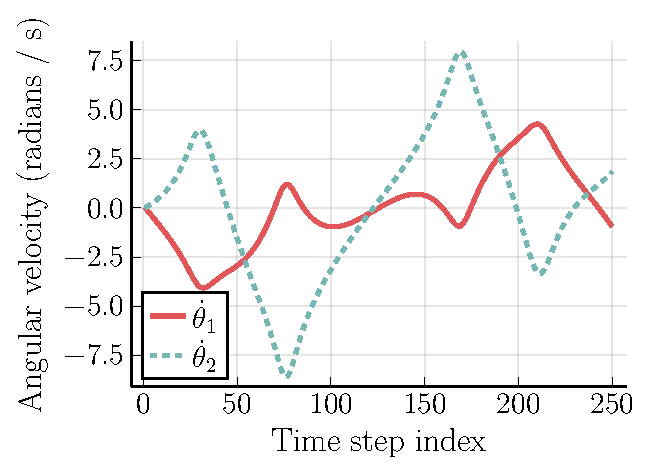
\includegraphics{contents/05-experiments/plots/nlds/03-pendulum_example_velocities.pdf}
    }
    \caption{Simulated evolution of the angular velocities $\dot{\theta}_1$ and $\dot{\theta}_2$ at each time step index $t$.}
    \label{fig:sim:pendulum_example_velocities}
  \end{subfigure}
  \caption{Simulated evolution of the double pendulum system state $s_t = (\theta_1, \theta_2, \dot{\theta}_1, \dot{\theta}_2)_t$ using the Runge-Kutta (RK4) method with a starting point of $s_1 = (1.2, 0.2, 0.0, 0.0)$ in discrete time steps.
    The time difference between measurements is set to be $0.01$ seconds.
    The masses $m_1$ and $m_2$ are set to be $14.715$ and $4.905$ respectively.
    The lengths $l_1$ and $l_2$ are equal and set to be $1.0$.
    The measurements $y$ only include the second component of the state vector.
    Other components of the state vector are not observed.
    The state transition noise $v$ is distributed according to the multivariate Normal
    distribution $\mathcal{N}(0, \Sigma)$, where the covariance matrix $\Sigma$ is a diagonal
    matrix with $10^{-6}$ values on the diagonal.
    The measurement noise signal $w$ is distributed according to the Normal distribution
    $\mathcal{N}(0, \Omega)$, where the variance $\Omega$ is set to be $0.3$.
    The figure shows the first $250$ time steps of the simulation.
  }
  \label{fig:sim:pendulum_example_states}
\end{figure}

%\begin{figure}
%\centering
%\resizebox{0.95\textwidth}{!}{% Recommended preamble:
% \usetikzlibrary{arrows.meta}
% \usetikzlibrary{backgrounds}
% \usepgfplotslibrary{patchplots}
% \usepgfplotslibrary{fillbetween}
% \pgfplotsset{%
%     layers/standard/.define layer set={%
%         background,axis background,axis grid,axis ticks,axis lines,axis tick labels,pre main,main,axis descriptions,axis foreground%
%     }{
%         grid style={/pgfplots/on layer=axis grid},%
%         tick style={/pgfplots/on layer=axis ticks},%
%         axis line style={/pgfplots/on layer=axis lines},%
%         label style={/pgfplots/on layer=axis descriptions},%
%         legend style={/pgfplots/on layer=axis descriptions},%
%         title style={/pgfplots/on layer=axis descriptions},%
%         colorbar style={/pgfplots/on layer=axis descriptions},%
%         ticklabel style={/pgfplots/on layer=axis tick labels},%
%         axis background@ style={/pgfplots/on layer=axis background},%
%         3d box foreground style={/pgfplots/on layer=axis foreground},%
%     },
% }

\begin{tikzpicture}[/tikz/background rectangle/.style={fill={rgb,1:red,1.0;green,1.0;blue,1.0}, fill opacity={1.0}, draw opacity={1.0}}, show background rectangle]
\begin{axis}[point meta max={nan}, point meta min={nan}, legend cell align={left}, legend columns={1}, title={}, title style={at={{(0.5,1)}}, anchor={south}, font={{\fontsize{18 pt}{23.400000000000002 pt}\selectfont}}, color={rgb,1:red,0.0;green,0.0;blue,0.0}, draw opacity={1.0}, rotate={0.0}, align={center}}, legend style={color={rgb,1:red,0.0;green,0.0;blue,0.0}, draw opacity={1.0}, line width={1}, solid, fill={rgb,1:red,1.0;green,1.0;blue,1.0}, fill opacity={1.0}, text opacity={1.0}, font={{\fontsize{16 pt}{20.8 pt}\selectfont}}, text={rgb,1:red,0.0;green,0.0;blue,0.0}, cells={anchor={center}}, at={(0.98, 0.02)}, anchor={south east}}, axis background/.style={fill={rgb,1:red,1.0;green,1.0;blue,1.0}, opacity={1.0}}, anchor={north west}, xshift={1.0mm}, yshift={-1.0mm}, width={201.2mm}, height={74.2mm}, scaled x ticks={false}, xlabel={Time step index}, x tick style={color={rgb,1:red,0.0;green,0.0;blue,0.0}, opacity={1.0}}, x tick label style={color={rgb,1:red,0.0;green,0.0;blue,0.0}, opacity={1.0}, rotate={0}}, xlabel style={at={(ticklabel cs:0.5)}, anchor=near ticklabel, at={{(ticklabel cs:0.5)}}, anchor={near ticklabel}, font={{\fontsize{18 pt}{23.400000000000002 pt}\selectfont}}, color={rgb,1:red,0.0;green,0.0;blue,0.0}, draw opacity={1.0}, rotate={0.0}}, xmajorgrids={true}, xmin={-13.970000000000027}, xmax={514.97}, xticklabels={{$0$,$100$,$200$,$300$,$400$,$500$}}, xtick={{0.0,100.0,200.0,300.0,400.0,500.0}}, xtick align={inside}, xticklabel style={font={{\fontsize{16 pt}{20.8 pt}\selectfont}}, color={rgb,1:red,0.0;green,0.0;blue,0.0}, draw opacity={1.0}, rotate={0.0}}, x grid style={color={rgb,1:red,0.0;green,0.0;blue,0.0}, draw opacity={0.1}, line width={0.5}, solid}, axis x line*={left}, x axis line style={color={rgb,1:red,0.0;green,0.0;blue,0.0}, draw opacity={1.0}, line width={1}, solid}, scaled y ticks={false}, ylabel={Angle (radians)}, y tick style={color={rgb,1:red,0.0;green,0.0;blue,0.0}, opacity={1.0}}, y tick label style={color={rgb,1:red,0.0;green,0.0;blue,0.0}, opacity={1.0}, rotate={0}}, ylabel style={at={(ticklabel cs:0.5)}, anchor=near ticklabel, at={{(ticklabel cs:0.5)}}, anchor={near ticklabel}, font={{\fontsize{18 pt}{23.400000000000002 pt}\selectfont}}, color={rgb,1:red,0.0;green,0.0;blue,0.0}, draw opacity={1.0}, rotate={0.0}}, ymajorgrids={true}, ymin={-3.1627985685809996}, ymax={4.001398297675946}, yticklabels={{$-2$,$0$,$2$,$4$}}, ytick={{-2.0,0.0,2.0,4.0}}, ytick align={inside}, yticklabel style={font={{\fontsize{16 pt}{20.8 pt}\selectfont}}, color={rgb,1:red,0.0;green,0.0;blue,0.0}, draw opacity={1.0}, rotate={0.0}}, y grid style={color={rgb,1:red,0.0;green,0.0;blue,0.0}, draw opacity={0.1}, line width={0.5}, solid}, axis y line*={left}, y axis line style={color={rgb,1:red,0.0;green,0.0;blue,0.0}, draw opacity={1.0}, line width={1}, solid}, colorbar={false}]
    \addplot[color={rgb,1:red,0.349;green,0.6314;blue,0.3098}, name path={20e679cb-e292-4d72-a30f-3c01ec8a30d4}, only marks, draw opacity={1.0}, line width={0}, solid, mark={*}, mark size={1.5 pt}, mark repeat={1}, mark options={color={rgb,1:red,0.0;green,0.0;blue,0.0}, draw opacity={1.0}, fill={rgb,1:red,0.349;green,0.6314;blue,0.3098}, fill opacity={1.0}, line width={0.0}, rotate={0}, solid}]
        table[row sep={\\}]
        {
            \\
            1.0  0.2547037461634025  \\
            2.0  0.13257046233559705  \\
            3.0  -0.03776758991926968  \\
            4.0  0.09161371400759022  \\
            5.0  0.03580303079397851  \\
            6.0  0.5243201219639236  \\
            7.0  -0.8317678104217855  \\
            8.0  0.7337639757938248  \\
            9.0  0.22525926075097388  \\
            10.0  0.060703235270812284  \\
            11.0  1.1737933912733125  \\
            12.0  0.7293091316300014  \\
            13.0  0.4526942096503235  \\
            14.0  0.23733115525947865  \\
            15.0  0.10045711610050653  \\
            16.0  0.010002203005235799  \\
            17.0  0.5849716363761392  \\
            18.0  1.0358206629387468  \\
            19.0  -0.06737686312785268  \\
            20.0  0.8199790894376653  \\
            21.0  0.11075360934320727  \\
            22.0  0.13090376179252466  \\
            23.0  0.6199697498576933  \\
            24.0  0.47159275449181753  \\
            25.0  0.5929405416150995  \\
            26.0  -1.2135665373223106  \\
            27.0  -0.44866295973229275  \\
            28.0  1.3265840688107517  \\
            29.0  -0.36583305536554445  \\
            30.0  0.949304748387459  \\
            31.0  1.1280175834461463  \\
            32.0  -0.18824106990492295  \\
            33.0  1.1197643355571476  \\
            34.0  0.5492803261703256  \\
            35.0  0.7686902631208499  \\
            36.0  0.3711370099283624  \\
            37.0  1.5122590414691222  \\
            38.0  0.6389043165711847  \\
            39.0  1.7274218873887848  \\
            40.0  0.7571412667515867  \\
            41.0  0.8204111857224877  \\
            42.0  0.7358486110893316  \\
            43.0  0.4968958503130323  \\
            44.0  2.5685992967612394  \\
            45.0  1.406056678762214  \\
            46.0  -0.7143217877382071  \\
            47.0  1.4991134982528218  \\
            48.0  0.46361233396621204  \\
            49.0  -0.10732966757856954  \\
            50.0  0.005352002113944487  \\
            51.0  0.4302888807554356  \\
            52.0  1.7421359411792186  \\
            53.0  1.8204722216757916  \\
            54.0  2.4952368321404834  \\
            55.0  1.3370275881377172  \\
            56.0  0.3529439649780819  \\
            57.0  0.33008697408953047  \\
            58.0  0.6228590344824246  \\
            59.0  0.6456893503624443  \\
            60.0  -0.03454432042297306  \\
            61.0  1.3902048320595508  \\
            62.0  0.3946371884144047  \\
            63.0  -0.5108757055489302  \\
            64.0  -0.3413719851201213  \\
            65.0  0.11345939121094634  \\
            66.0  -0.06852280893165702  \\
            67.0  1.042928613543596  \\
            68.0  0.016429464666352145  \\
            69.0  -0.6325896533488691  \\
            70.0  0.7132531520286924  \\
            71.0  -0.2589576993379058  \\
            72.0  -0.3270350833595384  \\
            73.0  -0.9987946037390639  \\
            74.0  0.08700004838123115  \\
            75.0  -0.8414776367231596  \\
            76.0  -0.9661575945971216  \\
            77.0  -0.3973354477736911  \\
            78.0  -0.9612560502306002  \\
            79.0  -0.10336496442805954  \\
            80.0  -0.09609815268853472  \\
            81.0  -1.1592087786938123  \\
            82.0  -1.752612003763668  \\
            83.0  -1.1469312919276016  \\
            84.0  -0.47904067512064585  \\
            85.0  0.10934428785343453  \\
            86.0  -1.1814654323630396  \\
            87.0  -1.7847524419801517  \\
            88.0  -1.0446277627615885  \\
            89.0  -1.8202833045766815  \\
            90.0  -1.3618410397311158  \\
            91.0  -1.6615797777525465  \\
            92.0  -0.20041513781277365  \\
            93.0  -1.8066344946051562  \\
            94.0  -1.9973256250305298  \\
            95.0  -1.5276086342422077  \\
            96.0  -1.9069607291602308  \\
            97.0  -2.283888732889661  \\
            98.0  -1.7495055467102847  \\
            99.0  -1.280413978460448  \\
            100.0  -1.794527938788751  \\
            101.0  -0.9350793519095448  \\
            102.0  -1.7801702059944355  \\
            103.0  -1.3307663563417451  \\
            104.0  -2.4753523322202415  \\
            105.0  -1.405132012217344  \\
            106.0  -1.2928011724102173  \\
            107.0  -1.6083470684035137  \\
            108.0  -1.6917811864631256  \\
            109.0  -1.120361859962426  \\
            110.0  -2.030965288679942  \\
            111.0  -2.242777682861987  \\
            112.0  -1.6518689048681314  \\
            113.0  -2.2793768057160637  \\
            114.0  -1.8821228665101208  \\
            115.0  -2.6957631794674164  \\
            116.0  -1.7461509806630824  \\
            117.0  -2.1419322564559584  \\
            118.0  -2.9600382799133507  \\
            119.0  -1.549348642096706  \\
            120.0  -1.7786924083727553  \\
            121.0  -2.279279300137501  \\
            122.0  -1.4197770384800101  \\
            123.0  -2.4870009676186786  \\
            124.0  -1.8939187940668558  \\
            125.0  -1.1452780024184255  \\
            126.0  -1.762804657436483  \\
            127.0  -2.958358586447785  \\
            128.0  -1.9678753036282253  \\
            129.0  -1.2866120734788664  \\
            130.0  -2.6288486206158783  \\
            131.0  -2.1318523277248858  \\
            132.0  -1.6020497590171445  \\
            133.0  -1.9787588277831722  \\
            134.0  -1.1479390192078547  \\
            135.0  -1.265486139945545  \\
            136.0  -2.1802697522359984  \\
            137.0  -1.9517398595235642  \\
            138.0  -1.7475681174680806  \\
            139.0  -1.9833710265259836  \\
            140.0  -2.1490718382039655  \\
            141.0  -1.3291352355050958  \\
            142.0  -1.743851573349185  \\
            143.0  -1.3600481155221495  \\
            144.0  -1.7714493216840912  \\
            145.0  -0.8962415563893462  \\
            146.0  -0.8234230389913816  \\
            147.0  -2.324907308996061  \\
            148.0  -1.254133825881493  \\
            149.0  -1.6097525414786458  \\
            150.0  -0.578114139934352  \\
            151.0  -1.3239620059485115  \\
            152.0  -0.7243928919061647  \\
            153.0  -1.283410064621941  \\
            154.0  -1.7473270629033948  \\
            155.0  -0.6986673644819154  \\
            156.0  -1.8626151500844275  \\
            157.0  -1.9347445137447257  \\
            158.0  -0.842063234393021  \\
            159.0  -2.05895557547552  \\
            160.0  -1.0435751654902805  \\
            161.0  -2.021011187277641  \\
            162.0  0.04549998660082011  \\
            163.0  -0.792534551761701  \\
            164.0  -0.9068480486991035  \\
            165.0  -0.2262425834735241  \\
            166.0  -0.9518746721201454  \\
            167.0  -0.22718942854916757  \\
            168.0  -0.08412107533518237  \\
            169.0  -1.3775567238188153  \\
            170.0  -0.5773270441455716  \\
            171.0  0.4548574286780537  \\
            172.0  -0.4913342999311329  \\
            173.0  -1.5196404104094683  \\
            174.0  0.04670881449122884  \\
            175.0  -0.03981830747880498  \\
            176.0  -0.03051172022122728  \\
            177.0  -0.7666882010123338  \\
            178.0  -0.8514670831496012  \\
            179.0  -0.31112845208766404  \\
            180.0  0.23461705449331224  \\
            181.0  -0.5667738317603577  \\
            182.0  0.3957519902448624  \\
            183.0  0.7909567080577389  \\
            184.0  0.35341347958062397  \\
            185.0  1.1364681196456983  \\
            186.0  -0.8866984983949993  \\
            187.0  0.8355489057574816  \\
            188.0  1.4286726142240131  \\
            189.0  0.6967053593922535  \\
            190.0  0.13057315453066154  \\
            191.0  0.003951425711167467  \\
            192.0  0.12893881621325853  \\
            193.0  0.3418514828675006  \\
            194.0  0.6623690670745918  \\
            195.0  0.971115257437804  \\
            196.0  0.8675616707231275  \\
            197.0  1.659762788216834  \\
            198.0  -0.22980701221832445  \\
            199.0  0.8158018319882907  \\
            200.0  1.1128360472584942  \\
            201.0  -0.29601005369727285  \\
            202.0  0.7023766852736714  \\
            203.0  0.9293406180086811  \\
            204.0  0.29015371371690346  \\
            205.0  0.7556310056529474  \\
            206.0  1.4344105171084804  \\
            207.0  1.4698620035432237  \\
            208.0  1.2941818852525873  \\
            209.0  0.3176034193205455  \\
            210.0  0.6785517639346975  \\
            211.0  0.792172500328094  \\
            212.0  1.2646419707916983  \\
            213.0  0.7960149273348547  \\
            214.0  0.3152646318989692  \\
            215.0  0.6548741529538871  \\
            216.0  -0.21144910077212714  \\
            217.0  -0.19414924581320875  \\
            218.0  -0.4740329810364304  \\
            219.0  0.9927697879645445  \\
            220.0  0.7241107825685815  \\
            221.0  1.6116659856676383  \\
            222.0  0.1350016249205366  \\
            223.0  0.6073804642947458  \\
            224.0  -0.6440673069791236  \\
            225.0  0.28335334619370584  \\
            226.0  0.35746396362649174  \\
            227.0  -0.4721405871607463  \\
            228.0  0.31718158750288894  \\
            229.0  0.9034357373574358  \\
            230.0  0.4162164899549826  \\
            231.0  0.6785569721554142  \\
            232.0  -0.7554189124192134  \\
            233.0  -0.07352504380112157  \\
            234.0  0.4799551408175747  \\
            235.0  0.6111606993526726  \\
            236.0  0.8035344971127392  \\
            237.0  0.4172396951092041  \\
            238.0  0.2264966528743171  \\
            239.0  -0.9837931596618397  \\
            240.0  0.49360922876195135  \\
            241.0  -0.20391346638707497  \\
            242.0  -0.04427114824239464  \\
            243.0  0.5320992830720863  \\
            244.0  0.7547897166086556  \\
            245.0  0.12664982304599093  \\
            246.0  -0.25291909862300027  \\
            247.0  0.05474471648881557  \\
            248.0  0.7012705881732797  \\
            249.0  1.1126540575872577  \\
            250.0  0.9564509782059143  \\
            251.0  0.6086049342251145  \\
            252.0  0.36497917307272715  \\
            253.0  0.8107120223693237  \\
            254.0  -0.14022250368494682  \\
            255.0  -0.5567382267815906  \\
            256.0  2.042790666922171  \\
            257.0  0.28553466984456144  \\
            258.0  1.0556365973219524  \\
            259.0  0.34777014128007483  \\
            260.0  -0.18067156125584405  \\
            261.0  1.997332567858869  \\
            262.0  1.684860640174111  \\
            263.0  0.12781814933239244  \\
            264.0  0.9343981681768515  \\
            265.0  0.8918032967660761  \\
            266.0  0.46063174159636844  \\
            267.0  0.7148957229897894  \\
            268.0  0.8443678383635875  \\
            269.0  0.8841012329654054  \\
            270.0  1.595037634437785  \\
            271.0  0.9208737925369979  \\
            272.0  1.706996691692529  \\
            273.0  2.2546304108994804  \\
            274.0  2.0122559426806443  \\
            275.0  1.3866010921131795  \\
            276.0  0.4660724748335717  \\
            277.0  1.6597815170707642  \\
            278.0  2.1037716408757894  \\
            279.0  1.0953964595497925  \\
            280.0  1.5607946722551016  \\
            281.0  0.9414944402504257  \\
            282.0  0.5607578326192387  \\
            283.0  1.4278986129947961  \\
            284.0  2.076966846601141  \\
            285.0  1.3999069772729673  \\
            286.0  0.8150626347309256  \\
            287.0  0.5485022388438334  \\
            288.0  1.5059141464901211  \\
            289.0  0.7290835898276607  \\
            290.0  1.6049076623581637  \\
            291.0  1.5697447834792064  \\
            292.0  0.45171024839277607  \\
            293.0  0.8293124007853085  \\
            294.0  0.846601310395398  \\
            295.0  0.8739146920926135  \\
            296.0  0.08488410227529886  \\
            297.0  0.002190553834938269  \\
            298.0  0.5598896749165143  \\
            299.0  0.6488627031233556  \\
            300.0  0.6626201431943712  \\
            301.0  1.550809263129851  \\
            302.0  1.2035366486807428  \\
            303.0  1.4391513598957628  \\
            304.0  0.9465325080806437  \\
            305.0  1.0363051989532819  \\
            306.0  0.23808535182725732  \\
            307.0  0.6627634639145569  \\
            308.0  0.07281148228098394  \\
            309.0  -0.5777034836980899  \\
            310.0  -0.12292021554616031  \\
            311.0  1.0502619194373501  \\
            312.0  -0.45659941413233857  \\
            313.0  0.15183854869504282  \\
            314.0  -0.6863180564401987  \\
            315.0  0.3230755997005984  \\
            316.0  -0.9453184589914141  \\
            317.0  -0.4585674228477514  \\
            318.0  -1.3071798370154104  \\
            319.0  -0.4978799443024999  \\
            320.0  -0.4088673706448102  \\
            321.0  -0.3128210562588147  \\
            322.0  -1.146473803498684  \\
            323.0  -0.7587892155610564  \\
            324.0  -1.4263939872180178  \\
            325.0  -0.7074078532701644  \\
            326.0  -1.022633900769508  \\
            327.0  -0.98774822932522  \\
            328.0  -0.6916193332964828  \\
            329.0  -2.0016733429279228  \\
            330.0  -1.4131814744671165  \\
            331.0  -1.7930584486992707  \\
            332.0  -1.0855561768133115  \\
            333.0  -1.7393989295487908  \\
            334.0  -1.3819726354505815  \\
            335.0  -1.1648785058254565  \\
            336.0  -1.1696073623634942  \\
            337.0  -2.22389591886838  \\
            338.0  -1.436309384075033  \\
            339.0  -1.4251929505875185  \\
            340.0  -2.776049799437655  \\
            341.0  -2.015551359451244  \\
            342.0  -1.4453997369175922  \\
            343.0  -1.6318896644401617  \\
            344.0  -1.3405557295883137  \\
            345.0  -1.938032837095029  \\
            346.0  -1.1602399262184786  \\
            347.0  -2.2341320955057733  \\
            348.0  -2.023659457762066  \\
            349.0  -1.3512464239084263  \\
            350.0  -1.2546849565308018  \\
            351.0  -2.789860757175241  \\
            352.0  -2.1450923087806646  \\
            353.0  -1.4082746958849548  \\
            354.0  -2.124991790703219  \\
            355.0  -2.524805156615292  \\
            356.0  -1.3570631992843396  \\
            357.0  -2.1583761447926655  \\
            358.0  -1.4119514670359934  \\
            359.0  -2.6025322083758513  \\
            360.0  -2.2737146590008903  \\
            361.0  -0.9001825844007502  \\
            362.0  -1.573369654329728  \\
            363.0  -0.599429902944882  \\
            364.0  -1.4189348800495303  \\
            365.0  -1.4594283988176981  \\
            366.0  -1.442131238522419  \\
            367.0  -1.9203528374277246  \\
            368.0  -2.163109350493304  \\
            369.0  -1.6720797183679454  \\
            370.0  -2.3683604047124254  \\
            371.0  -1.8192560001767353  \\
            372.0  -1.8596849452131368  \\
            373.0  -2.133720376870821  \\
            374.0  -2.1572688262127735  \\
            375.0  -2.0132201429760843  \\
            376.0  -2.251616277999592  \\
            377.0  -1.6512530881801881  \\
            378.0  -2.5752184245881256  \\
            379.0  -1.4988184096798005  \\
            380.0  -1.5770600580654228  \\
            381.0  -1.4176315937500161  \\
            382.0  -0.3842147119966244  \\
            383.0  -1.3145227316277073  \\
            384.0  -1.5181413561303954  \\
            385.0  -0.9843052329262914  \\
            386.0  -1.3493778679300799  \\
            387.0  -0.8600089106646416  \\
            388.0  -0.9397972935597814  \\
            389.0  -1.647682186971911  \\
            390.0  -0.24146190170522108  \\
            391.0  -1.149427215835684  \\
            392.0  -0.6135056898672351  \\
            393.0  -0.23704227857604454  \\
            394.0  -0.7266293222284332  \\
            395.0  -0.6469705578152578  \\
            396.0  -0.3302973842437824  \\
            397.0  0.026955363776290597  \\
            398.0  -0.6066017396824744  \\
            399.0  -0.28600718047321994  \\
            400.0  -0.4411287947197255  \\
            401.0  -0.8407578459391283  \\
            402.0  -0.8566991229381864  \\
            403.0  -0.11663955661405484  \\
            404.0  -0.2318327999287174  \\
            405.0  -1.3079709713328675  \\
            406.0  -0.373487161529459  \\
            407.0  -0.7188321977668082  \\
            408.0  -0.23123651433818074  \\
            409.0  -0.1856290459735493  \\
            410.0  -0.540336242094907  \\
            411.0  0.8337033209990051  \\
            412.0  -0.3396091540246816  \\
            413.0  -0.42910998394416744  \\
            414.0  -0.09462292850916931  \\
            415.0  -0.15017075721075504  \\
            416.0  0.41213988117037437  \\
            417.0  0.36491289243153135  \\
            418.0  0.337896049834181  \\
            419.0  -0.14159182180049262  \\
            420.0  0.3100023522725418  \\
            421.0  -0.15411792005010652  \\
            422.0  -0.04805806938270364  \\
            423.0  -0.1694380388120736  \\
            424.0  -0.20075377742702127  \\
            425.0  -0.008950829491479642  \\
            426.0  -0.4149538639880728  \\
            427.0  0.1315005462593218  \\
            428.0  -0.0978205171395651  \\
            429.0  -0.32781175892481035  \\
            430.0  -0.5416378726445532  \\
            431.0  -0.592027995888375  \\
            432.0  -0.0072412499821009335  \\
            433.0  1.0757461134062702  \\
            434.0  0.3187614023975534  \\
            435.0  -0.3462311843273594  \\
            436.0  0.7877353816789289  \\
            437.0  0.6063977877619431  \\
            438.0  -0.6253099371736408  \\
            439.0  -0.5251760267252457  \\
            440.0  -0.7042190087360131  \\
            441.0  0.501730289547447  \\
            442.0  -0.5432339546632522  \\
            443.0  0.46240715276019245  \\
            444.0  -1.3638831432538736  \\
            445.0  0.27692021444472936  \\
            446.0  -0.28368394816613585  \\
            447.0  0.03578460381578301  \\
            448.0  -0.22517247272992194  \\
            449.0  -0.5598223791153143  \\
            450.0  1.2340688123060086  \\
            451.0  0.7872944419691128  \\
            452.0  0.2722569244292567  \\
            453.0  0.4254568179708278  \\
            454.0  0.1969275217683756  \\
            455.0  1.133441032672545  \\
            456.0  0.6658599460644867  \\
            457.0  1.9985518620530995  \\
            458.0  0.016524650050032896  \\
            459.0  0.807295983156374  \\
            460.0  0.7250361007337011  \\
            461.0  0.5332407655761877  \\
            462.0  -0.7119212761095042  \\
            463.0  2.4026773260289414  \\
            464.0  0.029620102395093495  \\
            465.0  0.7926953815630983  \\
            466.0  2.0601968140143283  \\
            467.0  0.5597883347518665  \\
            468.0  0.2514432720609753  \\
            469.0  0.6302679706671976  \\
            470.0  1.108173209534797  \\
            471.0  0.8255730143149258  \\
            472.0  1.3672865928237867  \\
            473.0  2.127190053908513  \\
            474.0  0.7028778760573932  \\
            475.0  1.0740457652865356  \\
            476.0  1.3401585553280866  \\
            477.0  1.3221688074315678  \\
            478.0  2.0436794384366976  \\
            479.0  1.504102864120624  \\
            480.0  1.680958305960178  \\
            481.0  1.1510945551751592  \\
            482.0  1.0373728076856932  \\
            483.0  0.9736528078858427  \\
            484.0  2.323150574619187  \\
            485.0  1.6585870925096187  \\
            486.0  1.4809574354758377  \\
            487.0  0.4707693339277854  \\
            488.0  1.7715124020594613  \\
            489.0  2.2854953468975143  \\
            490.0  1.4861928161488789  \\
            491.0  1.5555742747797223  \\
            492.0  1.842983651332346  \\
            493.0  3.7986380090082967  \\
            494.0  2.6034814916128366  \\
            495.0  2.6757511607228572  \\
            496.0  1.6688285847992965  \\
            497.0  2.2405816958585785  \\
            498.0  1.9152722958693746  \\
            499.0  1.7944875204012671  \\
            500.0  1.960266375197512  \\
        }
        ;
    \addlegendentry {$y = \theta_2 + \omega$}
    \addplot[color={rgb,1:red,0.949;green,0.5569;blue,0.1686}, name path={d5feaefa-7394-43f6-b2be-5a8419165467}, draw opacity={1.0}, line width={2}, dashed]
        table[row sep={\\}]
        {
            \\
            1.0  0.2  \\
            2.0  0.20077121306979956  \\
            3.0  0.20244421310869218  \\
            4.0  0.20538450261381772  \\
            5.0  0.2076748169724466  \\
            6.0  0.21004613114216075  \\
            7.0  0.21198732109905916  \\
            8.0  0.21872872777404256  \\
            9.0  0.22323289221781725  \\
            10.0  0.22943985449754048  \\
            11.0  0.23581566502370901  \\
            12.0  0.24315735276246045  \\
            13.0  0.25284533768152134  \\
            14.0  0.26333740397862243  \\
            15.0  0.2767267762686036  \\
            16.0  0.29025284273577634  \\
            17.0  0.30537834643258177  \\
            18.0  0.3223457673611555  \\
            19.0  0.33790075820583876  \\
            20.0  0.35864484846938993  \\
            21.0  0.381008210128867  \\
            22.0  0.40503304101881643  \\
            23.0  0.4297012844324011  \\
            24.0  0.45813855895874606  \\
            25.0  0.48682693931483995  \\
            26.0  0.5206129038195051  \\
            27.0  0.5559471357422973  \\
            28.0  0.5922734827511258  \\
            29.0  0.6295904162401603  \\
            30.0  0.6681568582309619  \\
            31.0  0.7069617380962739  \\
            32.0  0.7458108999643405  \\
            33.0  0.7837109003387867  \\
            34.0  0.8199399855636275  \\
            35.0  0.8502841255822313  \\
            36.0  0.8783688485478693  \\
            37.0  0.9035997250689355  \\
            38.0  0.9251420935601686  \\
            39.0  0.9447342773893882  \\
            40.0  0.9621520056848557  \\
            41.0  0.9766089837799784  \\
            42.0  0.9890431780302547  \\
            43.0  0.9949241636544784  \\
            44.0  0.9969713618207969  \\
            45.0  0.9973295439251917  \\
            46.0  0.9932927022359279  \\
            47.0  0.9864562676330484  \\
            48.0  0.9780658607032465  \\
            49.0  0.9663855710137768  \\
            50.0  0.9536149015339549  \\
            51.0  0.9353859590904313  \\
            52.0  0.9147743221649417  \\
            53.0  0.8924033613981605  \\
            54.0  0.8670071208395579  \\
            55.0  0.8401128720204886  \\
            56.0  0.80859996527425  \\
            57.0  0.7750602396433758  \\
            58.0  0.7390795630859462  \\
            59.0  0.700158369569577  \\
            60.0  0.6588167666960625  \\
            61.0  0.6137401324392603  \\
            62.0  0.5654269061868354  \\
            63.0  0.5151341678076061  \\
            64.0  0.46252447496209453  \\
            65.0  0.40651420138940986  \\
            66.0  0.3505493080310132  \\
            67.0  0.2921725223792161  \\
            68.0  0.23005615438543553  \\
            69.0  0.16228513577315584  \\
            70.0  0.09250511552723756  \\
            71.0  0.019513296113997818  \\
            72.0  -0.057542073684514736  \\
            73.0  -0.137917451369763  \\
            74.0  -0.21952606427583504  \\
            75.0  -0.30457893498341554  \\
            76.0  -0.3915912846654537  \\
            77.0  -0.47728396192190414  \\
            78.0  -0.5636963639110109  \\
            79.0  -0.6444670567618447  \\
            80.0  -0.7239413402630823  \\
            81.0  -0.7989819317719744  \\
            82.0  -0.8715307328990217  \\
            83.0  -0.940233108432891  \\
            84.0  -1.005239787419807  \\
            85.0  -1.0685953502753918  \\
            86.0  -1.1283227352474465  \\
            87.0  -1.185359026976821  \\
            88.0  -1.2394906751023496  \\
            89.0  -1.2943304148202577  \\
            90.0  -1.3441062924771507  \\
            91.0  -1.3902859791631426  \\
            92.0  -1.4366803682827065  \\
            93.0  -1.4811529284215403  \\
            94.0  -1.5225448964617248  \\
            95.0  -1.563730261262378  \\
            96.0  -1.5997131249515735  \\
            97.0  -1.6366441866414128  \\
            98.0  -1.6733136776466513  \\
            99.0  -1.7056024983702138  \\
            100.0  -1.737847797377272  \\
            101.0  -1.768615713947156  \\
            102.0  -1.7973953650595775  \\
            103.0  -1.8266478016459915  \\
            104.0  -1.8525142454289871  \\
            105.0  -1.875355680191903  \\
            106.0  -1.8985285772418155  \\
            107.0  -1.9200193226034352  \\
            108.0  -1.9382098190965413  \\
            109.0  -1.955117629532639  \\
            110.0  -1.9696443312177885  \\
            111.0  -1.9839163127155266  \\
            112.0  -1.9971876830609512  \\
            113.0  -2.010110211562051  \\
            114.0  -2.0209182957170873  \\
            115.0  -2.0325631009319194  \\
            116.0  -2.0404197873851406  \\
            117.0  -2.047105285757217  \\
            118.0  -2.05406118715393  \\
            119.0  -2.0578465063172775  \\
            120.0  -2.061754863949012  \\
            121.0  -2.0623956324894124  \\
            122.0  -2.0635020145097647  \\
            123.0  -2.065016572927728  \\
            124.0  -2.0642986961816012  \\
            125.0  -2.062082836640928  \\
            126.0  -2.0572354604704226  \\
            127.0  -2.051457063599901  \\
            128.0  -2.0453135650132035  \\
            129.0  -2.0377082511655993  \\
            130.0  -2.0271684177566027  \\
            131.0  -2.0174163118592103  \\
            132.0  -2.006627255161083  \\
            133.0  -1.99458661776932  \\
            134.0  -1.981714592694915  \\
            135.0  -1.9657357644053175  \\
            136.0  -1.95008811649449  \\
            137.0  -1.9303573794981208  \\
            138.0  -1.9110237806162047  \\
            139.0  -1.891032236293788  \\
            140.0  -1.86892276396149  \\
            141.0  -1.8459024476627526  \\
            142.0  -1.8240516541245848  \\
            143.0  -1.7969981244184352  \\
            144.0  -1.7689196262694191  \\
            145.0  -1.7410262603456275  \\
            146.0  -1.7107785978513035  \\
            147.0  -1.6775932275228054  \\
            148.0  -1.6435335559227948  \\
            149.0  -1.6087777293433998  \\
            150.0  -1.5715761528918881  \\
            151.0  -1.5333355225829213  \\
            152.0  -1.4924470485598136  \\
            153.0  -1.4505696989582664  \\
            154.0  -1.4081074652001293  \\
            155.0  -1.3631752509782977  \\
            156.0  -1.315047608485016  \\
            157.0  -1.2671404222558629  \\
            158.0  -1.2145856333462213  \\
            159.0  -1.1590012892917456  \\
            160.0  -1.1007170055946283  \\
            161.0  -1.0412272270808436  \\
            162.0  -0.9788028842153407  \\
            163.0  -0.9154362282771672  \\
            164.0  -0.8467195634224802  \\
            165.0  -0.7740772228420397  \\
            166.0  -0.6991025525069955  \\
            167.0  -0.6219897733785096  \\
            168.0  -0.544075776265649  \\
            169.0  -0.4647533959092831  \\
            170.0  -0.3871719296897495  \\
            171.0  -0.30871861039755644  \\
            172.0  -0.23228660994473999  \\
            173.0  -0.16006993457316293  \\
            174.0  -0.09104079554576809  \\
            175.0  -0.023836038553904634  \\
            176.0  0.04065941764398388  \\
            177.0  0.10298433719679366  \\
            178.0  0.16191786460486846  \\
            179.0  0.21717664729431627  \\
            180.0  0.27196657770121696  \\
            181.0  0.32217097417301116  \\
            182.0  0.3704057719112007  \\
            183.0  0.41381936139150055  \\
            184.0  0.45562076321800266  \\
            185.0  0.4956701607299468  \\
            186.0  0.533427051320366  \\
            187.0  0.568639337023961  \\
            188.0  0.6009351087159419  \\
            189.0  0.6309386763830759  \\
            190.0  0.6559845555974834  \\
            191.0  0.6807106299250723  \\
            192.0  0.702832881211831  \\
            193.0  0.7215784638941529  \\
            194.0  0.7368913573391841  \\
            195.0  0.7489647617236266  \\
            196.0  0.7587190342979474  \\
            197.0  0.7647364823399241  \\
            198.0  0.7678485327456598  \\
            199.0  0.7664416622206628  \\
            200.0  0.7638649055908637  \\
            201.0  0.7571631057135545  \\
            202.0  0.7459260731431627  \\
            203.0  0.7330132005437374  \\
            204.0  0.7166998253727788  \\
            205.0  0.6970059767715231  \\
            206.0  0.6728385877341402  \\
            207.0  0.6478060532225469  \\
            208.0  0.6195863531767273  \\
            209.0  0.5868529561778992  \\
            210.0  0.5565162004508684  \\
            211.0  0.5235131226371783  \\
            212.0  0.49046125601779067  \\
            213.0  0.45908445524916563  \\
            214.0  0.4287847959908928  \\
            215.0  0.3998148291027864  \\
            216.0  0.37347240850929825  \\
            217.0  0.3480287471251013  \\
            218.0  0.3267248542670755  \\
            219.0  0.30876219079313677  \\
            220.0  0.29228402246562163  \\
            221.0  0.27752050815829726  \\
            222.0  0.2665193975217233  \\
            223.0  0.2587725529804194  \\
            224.0  0.2529307282775175  \\
            225.0  0.2483180748127668  \\
            226.0  0.2440885148853471  \\
            227.0  0.2427798059909984  \\
            228.0  0.2426666754505097  \\
            229.0  0.24357407307853082  \\
            230.0  0.24644402757467024  \\
            231.0  0.24939693899033108  \\
            232.0  0.2543840911518738  \\
            233.0  0.2601560785761774  \\
            234.0  0.2675938233072742  \\
            235.0  0.2761793284140923  \\
            236.0  0.2849108055903707  \\
            237.0  0.29213702863752405  \\
            238.0  0.30335718171378145  \\
            239.0  0.31517148765300046  \\
            240.0  0.3259089236880202  \\
            241.0  0.3399682838979915  \\
            242.0  0.352352226201167  \\
            243.0  0.36610976576424914  \\
            244.0  0.3811338156002569  \\
            245.0  0.39720331331081  \\
            246.0  0.41544809635028374  \\
            247.0  0.4342584566805917  \\
            248.0  0.45318580254310387  \\
            249.0  0.47051640079546203  \\
            250.0  0.4909670906812182  \\
            251.0  0.5123169411543128  \\
            252.0  0.5341537477526385  \\
            253.0  0.5573820680188972  \\
            254.0  0.5835830581812941  \\
            255.0  0.6107251247397203  \\
            256.0  0.6406161162667461  \\
            257.0  0.6702865430626567  \\
            258.0  0.7016032452233902  \\
            259.0  0.7347960859908554  \\
            260.0  0.7705628308338417  \\
            261.0  0.8059160272118696  \\
            262.0  0.84288803856595  \\
            263.0  0.8811221824524031  \\
            264.0  0.9198144901495555  \\
            265.0  0.95884434700868  \\
            266.0  0.9954583838804504  \\
            267.0  1.0298741377702962  \\
            268.0  1.0620963085025146  \\
            269.0  1.0939848148453273  \\
            270.0  1.1237094248280324  \\
            271.0  1.1499473336236519  \\
            272.0  1.1762164321933248  \\
            273.0  1.19810910993671  \\
            274.0  1.216592320085004  \\
            275.0  1.2340240970896694  \\
            276.0  1.2490729120116455  \\
            277.0  1.2616507087092939  \\
            278.0  1.2731459764365671  \\
            279.0  1.2790286057274227  \\
            280.0  1.2826761038801717  \\
            281.0  1.2818506515993286  \\
            282.0  1.2821127224324627  \\
            283.0  1.2780850357853335  \\
            284.0  1.271882537167133  \\
            285.0  1.2634332162823554  \\
            286.0  1.2525107018951074  \\
            287.0  1.2381118944893745  \\
            288.0  1.2226291302564298  \\
            289.0  1.2041263887955536  \\
            290.0  1.1820500585997478  \\
            291.0  1.1576983384623114  \\
            292.0  1.1307560022316532  \\
            293.0  1.1024438194823365  \\
            294.0  1.071669706706363  \\
            295.0  1.0368412239102822  \\
            296.0  0.9992564558933096  \\
            297.0  0.9611198859474601  \\
            298.0  0.9206250823234695  \\
            299.0  0.8754309651938195  \\
            300.0  0.8296117610952934  \\
            301.0  0.7816644017332739  \\
            302.0  0.7304266423142528  \\
            303.0  0.6756067306473944  \\
            304.0  0.6190265780459794  \\
            305.0  0.5584983854187708  \\
            306.0  0.4945959772946861  \\
            307.0  0.42809256646303506  \\
            308.0  0.35743390304190054  \\
            309.0  0.28237060763882155  \\
            310.0  0.20635408477251946  \\
            311.0  0.1250553670513947  \\
            312.0  0.04180154609516395  \\
            313.0  -0.04551155106840756  \\
            314.0  -0.1345143377334055  \\
            315.0  -0.22336764701950043  \\
            316.0  -0.3125542934537056  \\
            317.0  -0.4006237103481264  \\
            318.0  -0.48579671222006027  \\
            319.0  -0.5661325834512474  \\
            320.0  -0.6426821090518738  \\
            321.0  -0.7172673894809637  \\
            322.0  -0.7873213024989413  \\
            323.0  -0.8535899716351228  \\
            324.0  -0.9169131725885248  \\
            325.0  -0.9763768999174139  \\
            326.0  -1.0338852035448125  \\
            327.0  -1.0891228139966511  \\
            328.0  -1.1416932335586711  \\
            329.0  -1.193887252163816  \\
            330.0  -1.2430722378361234  \\
            331.0  -1.2883536780403297  \\
            332.0  -1.329396889152606  \\
            333.0  -1.3721015380533579  \\
            334.0  -1.410587058006288  \\
            335.0  -1.4492797618722968  \\
            336.0  -1.486674589986813  \\
            337.0  -1.5206389114801222  \\
            338.0  -1.5501233600278685  \\
            339.0  -1.5796125431703836  \\
            340.0  -1.605352478506891  \\
            341.0  -1.6305648993554678  \\
            342.0  -1.6556095801916717  \\
            343.0  -1.6776966573688799  \\
            344.0  -1.6997700496991055  \\
            345.0  -1.7191881263115145  \\
            346.0  -1.7369253843635197  \\
            347.0  -1.7515632743001506  \\
            348.0  -1.7643092546648584  \\
            349.0  -1.7755572892747071  \\
            350.0  -1.7858686698589785  \\
            351.0  -1.7934184436420966  \\
            352.0  -1.7990947955853844  \\
            353.0  -1.8028736089432493  \\
            354.0  -1.8053315454855539  \\
            355.0  -1.8079919924695234  \\
            356.0  -1.8093904029978138  \\
            357.0  -1.8078166392243034  \\
            358.0  -1.8055371340062794  \\
            359.0  -1.8019405037544185  \\
            360.0  -1.794975486009442  \\
            361.0  -1.7905792287527662  \\
            362.0  -1.7827217879847146  \\
            363.0  -1.772925501738634  \\
            364.0  -1.7632655353784426  \\
            365.0  -1.7520106091188579  \\
            366.0  -1.7383000493614214  \\
            367.0  -1.7234026804900597  \\
            368.0  -1.708974424622292  \\
            369.0  -1.69236497220162  \\
            370.0  -1.6755435472232991  \\
            371.0  -1.6571146092150943  \\
            372.0  -1.6374132718613716  \\
            373.0  -1.6163102211069915  \\
            374.0  -1.5929513801862383  \\
            375.0  -1.5687634294720114  \\
            376.0  -1.5428182225696192  \\
            377.0  -1.514806187896199  \\
            378.0  -1.4864729695322472  \\
            379.0  -1.4598740006553625  \\
            380.0  -1.428238813862558  \\
            381.0  -1.3966106475504818  \\
            382.0  -1.3633237176332025  \\
            383.0  -1.3297460029459516  \\
            384.0  -1.2927014569083286  \\
            385.0  -1.2559255313171707  \\
            386.0  -1.2176065190303096  \\
            387.0  -1.177734348758448  \\
            388.0  -1.1380828389474167  \\
            389.0  -1.0965241030332809  \\
            390.0  -1.0544048855806913  \\
            391.0  -1.0104318668487824  \\
            392.0  -0.9668637422171491  \\
            393.0  -0.9210986512713824  \\
            394.0  -0.8759473281918401  \\
            395.0  -0.8308703080506649  \\
            396.0  -0.7879880374857822  \\
            397.0  -0.7426043444842876  \\
            398.0  -0.6983254732221218  \\
            399.0  -0.6550811625572704  \\
            400.0  -0.6132201649598005  \\
            401.0  -0.5706226728514276  \\
            402.0  -0.5322993731682073  \\
            403.0  -0.49292381085620945  \\
            404.0  -0.4577807272342732  \\
            405.0  -0.4229313927409816  \\
            406.0  -0.38872015090073975  \\
            407.0  -0.35614586208550836  \\
            408.0  -0.32391746151118594  \\
            409.0  -0.2961991504149649  \\
            410.0  -0.2688703373225751  \\
            411.0  -0.24300339968906806  \\
            412.0  -0.21841312482110195  \\
            413.0  -0.195745558629374  \\
            414.0  -0.1758067598105461  \\
            415.0  -0.15669856498070192  \\
            416.0  -0.14225439628330064  \\
            417.0  -0.1296002340183511  \\
            418.0  -0.1183458774384559  \\
            419.0  -0.10776289230030738  \\
            420.0  -0.09928133750765428  \\
            421.0  -0.09505392176962664  \\
            422.0  -0.0907450575845551  \\
            423.0  -0.0875819912094041  \\
            424.0  -0.08625446621392481  \\
            425.0  -0.08602303669183034  \\
            426.0  -0.08713274729147846  \\
            427.0  -0.08967431522213234  \\
            428.0  -0.09140430098031307  \\
            429.0  -0.09296106125317692  \\
            430.0  -0.09622687805733805  \\
            431.0  -0.09684639699937946  \\
            432.0  -0.09642500882333452  \\
            433.0  -0.0967136950350474  \\
            434.0  -0.09573907530773336  \\
            435.0  -0.09341218857559279  \\
            436.0  -0.0904342350941615  \\
            437.0  -0.08456954983150432  \\
            438.0  -0.07583762207941781  \\
            439.0  -0.06742353933148973  \\
            440.0  -0.05631315723911538  \\
            441.0  -0.040785202322536226  \\
            442.0  -0.0235748776051294  \\
            443.0  -0.004782089065188591  \\
            444.0  0.01590566076613401  \\
            445.0  0.03950056776861398  \\
            446.0  0.06543046370744351  \\
            447.0  0.09492198194121704  \\
            448.0  0.12610558953312836  \\
            449.0  0.1586309851294126  \\
            450.0  0.19355706702781691  \\
            451.0  0.230025694199613  \\
            452.0  0.2679324797687284  \\
            453.0  0.3064775006398816  \\
            454.0  0.3482269644060056  \\
            455.0  0.39180595773331695  \\
            456.0  0.4350604666675338  \\
            457.0  0.4795282897482437  \\
            458.0  0.5257240292112495  \\
            459.0  0.5734869196666108  \\
            460.0  0.6223792324979419  \\
            461.0  0.6705189697226674  \\
            462.0  0.7192056655973864  \\
            463.0  0.7692543645849823  \\
            464.0  0.819610148030468  \\
            465.0  0.8695307437193631  \\
            466.0  0.9174735544541  \\
            467.0  0.9636516621615923  \\
            468.0  1.008535049737471  \\
            469.0  1.052868083983837  \\
            470.0  1.0960269081926686  \\
            471.0  1.1395459744608987  \\
            472.0  1.1810358753381913  \\
            473.0  1.222315868793669  \\
            474.0  1.2609254354362214  \\
            475.0  1.2982144544178071  \\
            476.0  1.3325148108960736  \\
            477.0  1.365792021915171  \\
            478.0  1.3988889620021583  \\
            479.0  1.429979927736979  \\
            480.0  1.459990136142756  \\
            481.0  1.4888925458881535  \\
            482.0  1.5153678924227227  \\
            483.0  1.5421780279299844  \\
            484.0  1.5663501709612253  \\
            485.0  1.5895042054268662  \\
            486.0  1.6126836645202955  \\
            487.0  1.633957416388249  \\
            488.0  1.6536515230672766  \\
            489.0  1.6717639042044081  \\
            490.0  1.6870349753785274  \\
            491.0  1.7031595765222853  \\
            492.0  1.7191392810467103  \\
            493.0  1.7320970606146595  \\
            494.0  1.746670888367036  \\
            495.0  1.7600274770352307  \\
            496.0  1.7697038593710774  \\
            497.0  1.7790393784436769  \\
            498.0  1.787770529010681  \\
            499.0  1.7958635671581844  \\
            500.0  1.8008777402744447  \\
        }
        ;
    \addlegendentry {$\theta_2$}
\end{axis}
\end{tikzpicture}
}
%\caption{Simulated measurements of the double pendulum system on Figure~\ref{fig:sim:pendulum_example_states}.
%We assume $g(s_t) = \theta_2$, thus measurements contain only a second component of the state
%vector.
%Other components of the state vector cannot be observed.
%The measurement noise $\omega$ is distributed according to the Normal distribution
%$\mathcal{N}(0, \Omega)$, where the variance $\Omega$ is set to be $0.3$.
%The figure shows only first $500$ time steps.
%}
%\label{fig:sim:pendulum_example_observations}
%\end{figure}

\subsection{The probabilistic model and the inference specification}

Listing~\ref{lst:sim:double_pendulum_model_specification} provides an example of the specification of the 
probabilistic model for the double pendulum system with nonlinear
dynamics~\eqref{eq:sim:nlds_model} using the RxInfer
framework.
\begin{figure*}
  \begin{adjustbox}{minipage=\textwidth,margin=0pt \smallskipamount,center}
    \jlinputlisting[label={lst:sim:double_pendulum_model_specification}, caption={
          An example of the specification of the probabilistic model for the double pendulum system with nonlinear dynamics~\eqref{eq:sim:nlds_model}.
        },captionpos=b]{contents/05-experiments/code/03-double-pendulum-model.jl}
  \end{adjustbox}
\end{figure*}
As part of the inference specification, we also introduce extra factorization constraints for
the variational family of distributions $Q_{B}$ using the \jlinl{@constraints} macro, as shown
in Listing~\eqref{lst:sim:double_pendulum_constraints}. 

These constraints assume that the states $\bm{s}$ and the precision of the measurement noise
are jointly independent.
\begin{figure*}
  \begin{adjustbox}{minipage=\textwidth,margin=0pt \smallskipamount,center}
    \jlinputlisting[label={lst:sim:double_pendulum_constraints}, caption={
          Extra factorization constraints for the variational family of distributions $Q_{B}$ in the probabilistic model of the double pendulum dynamics, which is defined in Listing~\eqref{lst:sim:double_pendulum_model_specification}.
        },captionpos=b]{contents/05-experiments/code/03-double-pendulum-constraints.jl}
  \end{adjustbox}
\end{figure*}
We utilize the \jlinl{@meta} macro to define an approximate inference strategy for the factor
$f$ in the model, as obtaining an exact solution is not feasible.
For our approximation method, we employ the \jlinl{Linearization()} method, which is a
first-order Taylor series expansion approximation.
The method locally approximates the nonlinearity with a linear function and performs exact
inference on the approximated factor \citep[Section~5.2]{sarkka_bayesian_2013}.
The \jlinl{Linearization()} method is provided by the RxInfer framework.
Other approximation strategies are possible, for example, Unscented transform
\citep[Section~5.5]{sarkka_bayesian_2013} or the Conjugate-Computation variational inference 
\citep{khan_conjugate-computation_2017,akbayrak_probabilistic_2022}.
\begin{figure*}
  \begin{adjustbox}{minipage=\textwidth,margin=0pt \smallskipamount,center}
    \jlinputlisting[label={lst:sim:double_pendulum_meta}, caption={
          Approximation method using \jlinl{Linearization()} for the nonlinear factor $f$ in the probabilistic model of the double pendulum dynamics defined in Listing~\eqref{lst:sim:double_pendulum_model_specification}.
          The \jlinl{Linearization()} method, which is a first-order Taylor series expansion approximation, is provided by the RxInfer framework.
        },captionpos=b]{contents/05-experiments/code/03-double-pendulum-meta.jl}
  \end{adjustbox}
\end{figure*}
In order to execute the inference procedure we simply call the \jlinl{inference()} function,
see Listing~\eqref{lst:sim:double_pendulum_inference}.
Figure~\ref{fig:sim:pendulum_example_inference_states} presents an example of the inference
task, showing the inferred posterior distributions over the states along with their
respective uncertainties.
Implementing the model and inference specifications for this type of model requires
approximately 30 lines of code (\hyperlink{experiments:userfriendliness}{\emph{User-friendliness}}).
\begin{figure*}
  \begin{adjustbox}{minipage=\textwidth,margin=0pt \smallskipamount,center}
    \jlinputlisting[label={lst:sim:double_pendulum_inference}, caption={
          An example of executing the inference procedure for the probabilistic model of the double pendulum dynamics defined in Listing~\eqref{lst:sim:double_pendulum_model_specification}, with constraints and approximation methods specified in Listing~\ref{lst:sim:double_pendulum_constraints} and Listing~\ref{lst:sim:double_pendulum_meta}, respectively.
        },captionpos=b]{contents/05-experiments/code/03-double-pendulum-inference.jl}
  \end{adjustbox}
\end{figure*}

%\begin{figure*}
%\begin{adjustbox}{minipage=\textwidth,margin=0pt \smallskipamount,center}
%\jlinputlisting[label={lst:sim:double_pendulum_full_example}, caption={An example of the probabilistic model and inference specification for the double pendulum non-linear dynamics~\eqref{eq:sim:nlds}-\eqref{eq:sim:pendulum_state_transition}.
%},captionpos=b]{contents/05-experiments/code/03-double-pendulum-full-example.jl}
%\end{adjustbox}
%\end{figure*}

\begin{figure}
  \centering
  \begin{subfigure}[t]{0.315\textwidth}
    \centering
    \resizebox{\textwidth}{!}{
        % % Recommended preamble:
% \usetikzlibrary{arrows.meta}
% \usetikzlibrary{backgrounds}
% \usepgfplotslibrary{patchplots}
% \usepgfplotslibrary{fillbetween}
% \pgfplotsset{%
%     layers/standard/.define layer set={%
%         background,axis background,axis grid,axis ticks,axis lines,axis tick labels,pre main,main,axis descriptions,axis foreground%
%     }{
%         grid style={/pgfplots/on layer=axis grid},%
%         tick style={/pgfplots/on layer=axis ticks},%
%         axis line style={/pgfplots/on layer=axis lines},%
%         label style={/pgfplots/on layer=axis descriptions},%
%         legend style={/pgfplots/on layer=axis descriptions},%
%         title style={/pgfplots/on layer=axis descriptions},%
%         colorbar style={/pgfplots/on layer=axis descriptions},%
%         ticklabel style={/pgfplots/on layer=axis tick labels},%
%         axis background@ style={/pgfplots/on layer=axis background},%
%         3d box foreground style={/pgfplots/on layer=axis foreground},%
%     },
% }

\begin{tikzpicture}[/tikz/background rectangle/.style={fill={rgb,1:red,1.0;green,1.0;blue,1.0}, fill opacity={1.0}, draw opacity={1.0}}, show background rectangle]
\begin{axis}[point meta max={nan}, point meta min={nan}, legend cell align={left}, legend columns={1}, title={}, title style={at={{(0.5,1)}}, anchor={south}, font={{\fontsize{18 pt}{23.400000000000002 pt}\selectfont}}, color={rgb,1:red,0.0;green,0.0;blue,0.0}, draw opacity={1.0}, rotate={0.0}, align={center}}, legend style={color={rgb,1:red,0.0;green,0.0;blue,0.0}, draw opacity={1.0}, line width={1}, solid, fill={rgb,1:red,1.0;green,1.0;blue,1.0}, fill opacity={1.0}, text opacity={1.0}, font={{\fontsize{14 pt}{18.2 pt}\selectfont}}, text={rgb,1:red,0.0;green,0.0;blue,0.0}, cells={anchor={center}}, at={(0.02, 0.02)}, anchor={south west}}, axis background/.style={fill={rgb,1:red,1.0;green,1.0;blue,1.0}, opacity={1.0}}, anchor={north west}, xshift={1.0mm}, yshift={-1.0mm}, width={99.6mm}, height={74.2mm}, scaled x ticks={false}, xlabel={Time step index}, x tick style={color={rgb,1:red,0.0;green,0.0;blue,0.0}, opacity={1.0}}, x tick label style={color={rgb,1:red,0.0;green,0.0;blue,0.0}, opacity={1.0}, rotate={0}}, xlabel style={at={(ticklabel cs:0.5)}, anchor=near ticklabel, at={{(ticklabel cs:0.5)}}, anchor={near ticklabel}, font={{\fontsize{16 pt}{20.8 pt}\selectfont}}, color={rgb,1:red,0.0;green,0.0;blue,0.0}, draw opacity={1.0}, rotate={0.0}}, xmajorgrids={true}, xmin={-6.469999999999999}, xmax={257.47}, xticklabels={{$0$,$50$,$100$,$150$,$200$,$250$}}, xtick={{0.0,50.0,100.0,150.0,200.0,250.0}}, xtick align={inside}, xticklabel style={font={{\fontsize{14 pt}{18.2 pt}\selectfont}}, color={rgb,1:red,0.0;green,0.0;blue,0.0}, draw opacity={1.0}, rotate={0.0}}, x grid style={color={rgb,1:red,0.0;green,0.0;blue,0.0}, draw opacity={0.1}, line width={0.5}, solid}, axis x line*={left}, x axis line style={color={rgb,1:red,0.0;green,0.0;blue,0.0}, draw opacity={1.0}, line width={1}, solid}, scaled y ticks={false}, ylabel={Angle (radians)}, y tick style={color={rgb,1:red,0.0;green,0.0;blue,0.0}, opacity={1.0}}, y tick label style={color={rgb,1:red,0.0;green,0.0;blue,0.0}, opacity={1.0}, rotate={0}}, ylabel style={at={(ticklabel cs:0.5)}, anchor=near ticklabel, at={{(ticklabel cs:0.5)}}, anchor={near ticklabel}, font={{\fontsize{16 pt}{20.8 pt}\selectfont}}, color={rgb,1:red,0.0;green,0.0;blue,0.0}, draw opacity={1.0}, rotate={0.0}}, ymajorgrids={true}, ymin={-4.064075544819777}, ymax={2.3669820967456285}, yticklabels={{$-4$,$-3$,$-2$,$-1$,$0$,$1$,$2$}}, ytick={{-4.0,-3.0,-2.0,-1.0,0.0,1.0,2.0}}, ytick align={inside}, yticklabel style={font={{\fontsize{14 pt}{18.2 pt}\selectfont}}, color={rgb,1:red,0.0;green,0.0;blue,0.0}, draw opacity={1.0}, rotate={0.0}}, y grid style={color={rgb,1:red,0.0;green,0.0;blue,0.0}, draw opacity={0.1}, line width={0.5}, solid}, axis y line*={left}, y axis line style={color={rgb,1:red,0.0;green,0.0;blue,0.0}, draw opacity={1.0}, line width={1}, solid}, colorbar={false}]
    \addplot+[line width={0}, draw opacity={0}, fill={rgb,1:red,0.8824;green,0.3412;blue,0.349}, fill opacity={0.5}, mark={none}, forget plot]
        coordinates {
            (1,1.1684620654295985)
            (2,1.1723934370800164)
            (3,1.174189896401998)
            (4,1.1742456488486275)
            (5,1.1725627849895122)
            (6,1.1691969857234075)
            (7,1.1641717510311234)
            (8,1.1574927864631517)
            (9,1.1491695495092458)
            (10,1.1391402878836963)
            (11,1.1273321405153243)
            (12,1.1136996165568733)
            (13,1.098348267838681)
            (14,1.0812207623594392)
            (15,1.0620165832945592)
            (16,1.0405921697456293)
            (17,1.0169219690399185)
            (18,0.9911319148636832)
            (19,0.9634854165117018)
            (20,0.9341082069087829)
            (21,0.9031059759877039)
            (22,0.8706007886354012)
            (23,0.8367268876695846)
            (24,0.8015972752852359)
            (25,0.7653753401433059)
            (26,0.7282696269701487)
            (27,0.6903483473595186)
            (28,0.6517633330445693)
            (29,0.6128816166922897)
            (30,0.5740128575430689)
            (31,0.5353689542893891)
            (32,0.49716100524022977)
            (33,0.45944415943711286)
            (34,0.42217991098603175)
            (35,0.3854015697437212)
            (36,0.349152577999913)
            (37,0.31344861985503586)
            (38,0.2782914106467327)
            (39,0.24367015593832586)
            (40,0.2095698380905346)
            (41,0.1759825270921614)
            (42,0.14289830719697763)
            (43,0.11031526303467981)
            (44,0.07823821157114501)
            (45,0.046668906347046235)
            (46,0.01562804472565035)
            (47,-0.014842266901310429)
            (48,-0.04469810306378706)
            (49,-0.07388871253824947)
            (50,-0.102355038834288)
            (51,-0.13003492774196324)
            (52,-0.1568597649340207)
            (53,-0.18275309419693803)
            (54,-0.20763327116265792)
            (55,-0.23141122597493688)
            (56,-0.2539936203149264)
            (57,-0.2752860399070448)
            (58,-0.29519578124546264)
            (59,-0.3136160252575994)
            (60,-0.330426247570315)
            (61,-0.34551392443985474)
            (62,-0.35877925445148035)
            (63,-0.3701353129036664)
            (64,-0.3794348375646544)
            (65,-0.38650560045414173)
            (66,-0.3912095788900051)
            (67,-0.3933703051109696)
            (68,-0.39284986650658543)
            (69,-0.3896246966970606)
            (70,-0.38368590070826425)
            (71,-0.37507420391896096)
            (72,-0.3641478663995805)
            (73,-0.351578300234441)
            (74,-0.3382054358314164)
            (75,-0.32498709451773705)
            (76,-0.3127383982822008)
            (77,-0.30203696300147453)
            (78,-0.29317908429058465)
            (79,-0.2861995810816395)
            (80,-0.2810805416183223)
            (81,-0.27777685741582586)
            (82,-0.27621551303521635)
            (83,-0.27630556132332673)
            (84,-0.27794294268188247)
            (85,-0.28099766259323417)
            (86,-0.2853316534570666)
            (87,-0.2908183201000722)
            (88,-0.29733482489042695)
            (89,-0.30475930960813274)
            (90,-0.3129744397086793)
            (91,-0.321882022495301)
            (92,-0.33139307179689903)
            (93,-0.34141783342333565)
            (94,-0.3518754453655576)
            (95,-0.36268604478433475)
            (96,-0.37376712402263357)
            (97,-0.38503942361659266)
            (98,-0.3964286994427101)
            (99,-0.40787077173874603)
            (100,-0.41931254624732667)
            (101,-0.4307024662433299)
            (102,-0.44198495427192486)
            (103,-0.45310707955558455)
            (104,-0.4640201829193735)
            (105,-0.4746785645225312)
            (106,-0.48504115686324906)
            (107,-0.4950676481182369)
            (108,-0.5047208333987061)
            (109,-0.5139679116554192)
            (110,-0.522778072622607)
            (111,-0.531124930658389)
            (112,-0.5389833020780798)
            (113,-0.5463282869424065)
            (114,-0.5531389242335379)
            (115,-0.5593989803832607)
            (116,-0.5650953572549223)
            (117,-0.5702170484901375)
            (118,-0.5747543121643969)
            (119,-0.578698796344267)
            (120,-0.5820442931128118)
            (121,-0.5847869310379269)
            (122,-0.5869254527034546)
            (123,-0.588459660837291)
            (124,-0.5893911687009826)
            (125,-0.5897239991744033)
            (126,-0.5894637728404195)
            (127,-0.5886174958627453)
            (128,-0.5871938258108506)
            (129,-0.5852053225787665)
            (130,-0.5826664594702683)
            (131,-0.5795913187951244)
            (132,-0.5759968600766823)
            (133,-0.5719024055110707)
            (134,-0.5673309144038609)
            (135,-0.5623073316174307)
            (136,-0.5568583711330003)
            (137,-0.5510141711625326)
            (138,-0.5448076620984703)
            (139,-0.5382733422918684)
            (140,-0.5314482034215263)
            (141,-0.5243712040313214)
            (142,-0.5170855360429609)
            (143,-0.509638459782994)
            (144,-0.5020815245658733)
            (145,-0.4944681784001883)
            (146,-0.4868530702276602)
            (147,-0.4792960860894861)
            (148,-0.47185801812751954)
            (149,-0.4646026153278246)
            (150,-0.45760094379784705)
            (151,-0.4509274275480017)
            (152,-0.44465944479219394)
            (153,-0.43887862996749905)
            (154,-0.43367229287421766)
            (155,-0.4291341659234812)
            (156,-0.42536202246626265)
            (157,-0.4224580567364321)
            (158,-0.42052756155762877)
            (159,-0.4196852411934716)
            (160,-0.4200511757642021)
            (161,-0.42173823289945966)
            (162,-0.4248220646686962)
            (163,-0.4293532073721908)
            (164,-0.4353540779023874)
            (165,-0.44273144451895413)
            (166,-0.45127767217092357)
            (167,-0.46065549510715725)
            (168,-0.47037434144631285)
            (169,-0.47981026472807875)
            (170,-0.4882990971011925)
            (171,-0.4952722273568802)
            (172,-0.5003109338296524)
            (173,-0.5031530179369117)
            (174,-0.5036710964735998)
            (175,-0.5018133949587681)
            (176,-0.49758795783854926)
            (177,-0.49104997948962065)
            (178,-0.4822805649024758)
            (179,-0.47136735620300835)
            (180,-0.45840303891462253)
            (181,-0.44348922862150125)
            (182,-0.42673318434826846)
            (183,-0.4082441709407492)
            (184,-0.388126354036324)
            (185,-0.3664600652045722)
            (186,-0.3433207254377717)
            (187,-0.318793354367488)
            (188,-0.2929597919529978)
            (189,-0.26589911383459697)
            (190,-0.2376871360785799)
            (191,-0.20839411057934856)
            (192,-0.17809357162293984)
            (193,-0.14684716104704448)
            (194,-0.11467884644416497)
            (195,-0.08160441260411126)
            (196,-0.04764066158510331)
            (197,-0.012799601374379101)
            (198,0.02291320853793495)
            (199,0.05949083934322415)
            (200,0.0969386738614862)
            (201,0.13528836439546876)
            (202,0.17457607728578872)
            (203,0.21483511612775055)
            (204,0.25606969231690624)
            (205,0.2982555150727469)
            (206,0.34134136264004816)
            (207,0.38525108346562675)
            (208,0.4298150753663038)
            (209,0.47474613787408004)
            (210,0.519662179295802)
            (211,0.5641349775847555)
            (212,0.6077480540018608)
            (213,0.6501353778470986)
            (214,0.6910160570979739)
            (215,0.7302194851356303)
            (216,0.7676610902649481)
            (217,0.803313715734488)
            (218,0.837192146825965)
            (219,0.8693366276072692)
            (220,0.8998017250650836)
            (221,0.9286460761418802)
            (222,0.9559257183272065)
            (223,0.9816923817060574)
            (224,1.00599301877092)
            (225,1.0288687000700112)
            (226,1.0503569874676457)
            (227,1.0704913356305026)
            (228,1.0892984942794903)
            (229,1.1068030351049116)
            (230,1.1230259311710469)
            (231,1.1379812828985796)
            (232,1.1516822862576344)
            (233,1.164137791158527)
            (234,1.1753526394455585)
            (235,1.1853346728307481)
            (236,1.1940911003633636)
            (237,1.2016274664821907)
            (238,1.2079441128466988)
            (239,1.2130372452422722)
            (240,1.216904397911528)
            (241,1.2195432793029775)
            (242,1.2209483179217793)
            (243,1.221111894754575)
            (244,1.2200243847274628)
            (245,1.2176722573206078)
            (246,1.2140423677578511)
            (247,1.2091189583574147)
            (248,1.2028842804702486)
            (249,1.1953181112993307)
            (250,1.1863949031211196)
            (250,0.8829227350024286)
            (249,0.8997327703409771)
            (248,0.9146817347985918)
            (247,0.9278247221116738)
            (246,0.939211290545604)
            (245,0.9488862231124804)
            (244,0.9568903825676558)
            (243,0.9632590518641351)
            (242,0.9680209199652252)
            (241,0.9712029014116159)
            (240,0.9728284723836037)
            (239,0.9729175041921824)
            (238,0.9714861584689571)
            (237,0.9685475580012655)
            (236,0.9641135846495825)
            (235,0.9581923302659874)
            (234,0.9507862199993218)
            (233,0.9418936305086925)
            (232,0.9315095462729228)
            (231,0.9196303683029575)
            (230,0.9062474619318501)
            (229,0.8913457524812081)
            (228,0.874907945474585)
            (227,0.8569053031912974)
            (226,0.837301407477547)
            (225,0.8160548860982224)
            (224,0.7931105531030156)
            (223,0.7684040388648377)
            (222,0.7418643110228459)
            (221,0.7134093254108391)
            (220,0.6829492313133928)
            (219,0.6503876273397429)
            (218,0.6156275905190167)
            (217,0.5785948543642859)
            (216,0.5392684736055074)
            (215,0.4977240317592756)
            (214,0.45414845048531993)
            (213,0.4088415009299732)
            (212,0.36232306603505715)
            (211,0.31540518128910106)
            (210,0.26888825988690773)
            (209,0.22345921648001915)
            (208,0.17962395282958904)
            (207,0.13766041874894083)
            (206,0.09756503478712503)
            (205,0.05894151741636888)
            (204,0.021428318904967714)
            (203,-0.01512712729133775)
            (202,-0.05091894604256869)
            (201,-0.08602762687094256)
            (200,-0.12044654612994908)
            (199,-0.15416702201582866)
            (198,-0.18717164472130682)
            (197,-0.2194354099537539)
            (196,-0.25092934056448407)
            (195,-0.28161547867660763)
            (194,-0.3114476263048334)
            (193,-0.34036922591785135)
            (192,-0.36832737779647917)
            (191,-0.39526567105084554)
            (190,-0.4211194913442867)
            (189,-0.445820113542975)
            (188,-0.4692984369612311)
            (187,-0.49148456612112423)
            (186,-0.5123098554150474)
            (185,-0.5317001511180599)
            (184,-0.5495789775827595)
            (183,-0.565880209224777)
            (182,-0.5805423434711947)
            (181,-0.5935135481994808)
            (180,-0.6047520393965465)
            (179,-0.6142308067089748)
            (178,-0.6219418968158841)
            (177,-0.6279076160236451)
            (176,-0.6321837030576181)
            (175,-0.63485404090369)
            (174,-0.6360260748586521)
            (173,-0.6358128961921561)
            (172,-0.6342697859223896)
            (171,-0.6313244294268272)
            (170,-0.626865918549339)
            (169,-0.6208665187440711)
            (168,-0.6136077211707504)
            (167,-0.6057346591246713)
            (166,-0.5980437476104716)
            (165,-0.5913241597275878)
            (164,-0.5861177415040597)
            (163,-0.5827703220156815)
            (162,-0.5813558392860136)
            (161,-0.5817796115775722)
            (160,-0.5839333863539903)
            (159,-0.5876623289082774)
            (158,-0.5927843526371944)
            (157,-0.5991171556264543)
            (156,-0.6064976799522791)
            (155,-0.6147820415399123)
            (154,-0.6238350976220294)
            (153,-0.6335305059879363)
            (152,-0.6437488571418424)
            (151,-0.6543819076937527)
            (150,-0.6653313224198067)
            (149,-0.6765051028388862)
            (148,-0.6878155018775505)
            (147,-0.6991790587553603)
            (146,-0.7105251168241334)
            (145,-0.7217878838830663)
            (144,-0.7329005031480358)
            (143,-0.7438045925626489)
            (142,-0.754442377106741)
            (141,-0.7647560592153777)
            (140,-0.7746946642519763)
            (139,-0.7842132504186441)
            (138,-0.793275600770722)
            (137,-0.8018462607966215)
            (136,-0.8098922075056172)
            (135,-0.8173801491989212)
            (134,-0.8242794346594957)
            (133,-0.8305665085619555)
            (132,-0.8362180748108765)
            (131,-0.8412115927870445)
            (130,-0.845531904587021)
            (129,-0.8491683408639351)
            (128,-0.852112977735054)
            (127,-0.8543533236890952)
            (126,-0.85587460175758)
            (125,-0.8566736162231864)
            (124,-0.8567464621284653)
            (123,-0.8560895082304667)
            (122,-0.854698291473617)
            (121,-0.8525721521759873)
            (120,-0.8497114671123474)
            (119,-0.8461150980095724)
            (118,-0.8417845143521236)
            (117,-0.8367254944386957)
            (116,-0.8309447271855952)
            (115,-0.8244500084168193)
            (114,-0.8172481494724664)
            (113,-0.809348902167669)
            (112,-0.8007655076175819)
            (111,-0.7915173971751343)
            (110,-0.7816282383836353)
            (109,-0.7711210815148274)
            (108,-0.7600185509475814)
            (107,-0.7483482904728445)
            (106,-0.7361399970604312)
            (105,-0.7234270039650452)
            (104,-0.710246591294601)
            (103,-0.6966369034372859)
            (102,-0.6826405496820378)
            (101,-0.6683035964030011)
            (100,-0.6536760627420193)
            (99,-0.6388117494478087)
            (98,-0.6237634639153944)
            (97,-0.6085859558651718)
            (96,-0.593343533511356)
            (95,-0.5781098556536404)
            (94,-0.5629639289374965)
            (93,-0.5479889654616501)
            (92,-0.5332686168017831)
            (91,-0.5188903747998066)
            (90,-0.5049504595803496)
            (89,-0.4915471298585508)
            (88,-0.478790353868647)
            (87,-0.4668073590385788)
            (86,-0.4557332492997831)
            (85,-0.4457103833895895)
            (84,-0.43689282240779503)
            (83,-0.4294541848223595)
            (82,-0.42356808417752134)
            (81,-0.4194124722421809)
            (80,-0.41716147627136874)
            (79,-0.41698909938537354)
            (78,-0.4190346213286292)
            (77,-0.42342268434304964)
            (76,-0.4301902130420908)
            (75,-0.43908952152998293)
            (74,-0.44958349959567945)
            (73,-0.4608505408048593)
            (72,-0.4720144567012352)
            (71,-0.48231749362020926)
            (70,-0.49120526434370915)
            (69,-0.4984721034781206)
            (68,-0.5040507688708085)
            (67,-0.5077579708851522)
            (66,-0.5094525400817447)
            (65,-0.5091036834384504)
            (64,-0.5067196292057784)
            (63,-0.5023091478229235)
            (62,-0.49595830442372724)
            (61,-0.4877548420162772)
            (60,-0.4777263072624712)
            (59,-0.46592592578459396)
            (58,-0.45243740756379336)
            (57,-0.43737100659021366)
            (56,-0.4208264806260655)
            (55,-0.4028849399824577)
            (54,-0.38363674693303607)
            (53,-0.3631790982758871)
            (52,-0.34160912188248543)
            (51,-0.3190156158946831)
            (50,-0.29548478925328014)
            (49,-0.2710935819438207)
            (48,-0.24591476212248348)
            (47,-0.2200263475962896)
            (46,-0.19349774748466578)
            (45,-0.16639397080495766)
            (44,-0.13878826727928123)
            (43,-0.11071499255029982)
            (42,-0.08216449536581669)
            (41,-0.053147992683330536)
            (40,-0.02367006204197758)
            (39,0.00632255371818774)
            (38,0.03686061508396102)
            (37,0.06794378583218375)
            (36,0.09962164678631619)
            (35,0.1319594539666979)
            (34,0.16501093740980471)
            (33,0.19881829044185)
            (32,0.233406050988411)
            (31,0.26880961197031056)
            (30,0.30505657834973793)
            (29,0.3420788991675071)
            (28,0.37974554446946934)
            (27,0.417754913288498)
            (26,0.45569980587387543)
            (25,0.49342920782802097)
            (24,0.5308964868985537)
            (23,0.5678381225782984)
            (22,0.6040278990369158)
            (21,0.639320405038813)
            (20,0.6735529645449354)
            (19,0.7065504090141721)
            (18,0.7381484117557555)
            (17,0.7681602858997012)
            (16,0.7962125618483642)
            (15,0.8220850575574473)
            (14,0.8456675012134012)
            (13,0.8669052702043317)
            (12,0.8859963367237453)
            (11,0.9030774236091625)
            (10,0.918130274957954)
            (9,0.9311912907443805)
            (8,0.942314499423422)
            (7,0.9515525880343685)
            (6,0.9588923281413013)
            (5,0.9643188112231794)
            (4,0.9678082350388932)
            (3,0.9693071287757883)
            (2,0.968813402378395)
            (1,0.9659791826877318)
            (1,1.1684620654295985)
        }
        ;
    \addplot+[line width={0}, draw opacity={0}, fill={rgb,1:red,0.8824;green,0.3412;blue,0.349}, fill opacity={0.5}, mark={none}, forget plot]
        coordinates {
            (1,1.1684620654295985)
            (2,1.1723934370800164)
            (3,1.174189896401998)
            (4,1.1742456488486275)
            (5,1.1725627849895122)
            (6,1.1691969857234075)
            (7,1.1641717510311234)
            (8,1.1574927864631517)
            (9,1.1491695495092458)
            (10,1.1391402878836963)
            (11,1.1273321405153243)
            (12,1.1136996165568733)
            (13,1.098348267838681)
            (14,1.0812207623594392)
            (15,1.0620165832945592)
            (16,1.0405921697456293)
            (17,1.0169219690399185)
            (18,0.9911319148636832)
            (19,0.9634854165117018)
            (20,0.9341082069087829)
            (21,0.9031059759877039)
            (22,0.8706007886354012)
            (23,0.8367268876695846)
            (24,0.8015972752852359)
            (25,0.7653753401433059)
            (26,0.7282696269701487)
            (27,0.6903483473595186)
            (28,0.6517633330445693)
            (29,0.6128816166922897)
            (30,0.5740128575430689)
            (31,0.5353689542893891)
            (32,0.49716100524022977)
            (33,0.45944415943711286)
            (34,0.42217991098603175)
            (35,0.3854015697437212)
            (36,0.349152577999913)
            (37,0.31344861985503586)
            (38,0.2782914106467327)
            (39,0.24367015593832586)
            (40,0.2095698380905346)
            (41,0.1759825270921614)
            (42,0.14289830719697763)
            (43,0.11031526303467981)
            (44,0.07823821157114501)
            (45,0.046668906347046235)
            (46,0.01562804472565035)
            (47,-0.014842266901310429)
            (48,-0.04469810306378706)
            (49,-0.07388871253824947)
            (50,-0.102355038834288)
            (51,-0.13003492774196324)
            (52,-0.1568597649340207)
            (53,-0.18275309419693803)
            (54,-0.20763327116265792)
            (55,-0.23141122597493688)
            (56,-0.2539936203149264)
            (57,-0.2752860399070448)
            (58,-0.29519578124546264)
            (59,-0.3136160252575994)
            (60,-0.330426247570315)
            (61,-0.34551392443985474)
            (62,-0.35877925445148035)
            (63,-0.3701353129036664)
            (64,-0.3794348375646544)
            (65,-0.38650560045414173)
            (66,-0.3912095788900051)
            (67,-0.3933703051109696)
            (68,-0.39284986650658543)
            (69,-0.3896246966970606)
            (70,-0.38368590070826425)
            (71,-0.37507420391896096)
            (72,-0.3641478663995805)
            (73,-0.351578300234441)
            (74,-0.3382054358314164)
            (75,-0.32498709451773705)
            (76,-0.3127383982822008)
            (77,-0.30203696300147453)
            (78,-0.29317908429058465)
            (79,-0.2861995810816395)
            (80,-0.2810805416183223)
            (81,-0.27777685741582586)
            (82,-0.27621551303521635)
            (83,-0.27630556132332673)
            (84,-0.27794294268188247)
            (85,-0.28099766259323417)
            (86,-0.2853316534570666)
            (87,-0.2908183201000722)
            (88,-0.29733482489042695)
            (89,-0.30475930960813274)
            (90,-0.3129744397086793)
            (91,-0.321882022495301)
            (92,-0.33139307179689903)
            (93,-0.34141783342333565)
            (94,-0.3518754453655576)
            (95,-0.36268604478433475)
            (96,-0.37376712402263357)
            (97,-0.38503942361659266)
            (98,-0.3964286994427101)
            (99,-0.40787077173874603)
            (100,-0.41931254624732667)
            (101,-0.4307024662433299)
            (102,-0.44198495427192486)
            (103,-0.45310707955558455)
            (104,-0.4640201829193735)
            (105,-0.4746785645225312)
            (106,-0.48504115686324906)
            (107,-0.4950676481182369)
            (108,-0.5047208333987061)
            (109,-0.5139679116554192)
            (110,-0.522778072622607)
            (111,-0.531124930658389)
            (112,-0.5389833020780798)
            (113,-0.5463282869424065)
            (114,-0.5531389242335379)
            (115,-0.5593989803832607)
            (116,-0.5650953572549223)
            (117,-0.5702170484901375)
            (118,-0.5747543121643969)
            (119,-0.578698796344267)
            (120,-0.5820442931128118)
            (121,-0.5847869310379269)
            (122,-0.5869254527034546)
            (123,-0.588459660837291)
            (124,-0.5893911687009826)
            (125,-0.5897239991744033)
            (126,-0.5894637728404195)
            (127,-0.5886174958627453)
            (128,-0.5871938258108506)
            (129,-0.5852053225787665)
            (130,-0.5826664594702683)
            (131,-0.5795913187951244)
            (132,-0.5759968600766823)
            (133,-0.5719024055110707)
            (134,-0.5673309144038609)
            (135,-0.5623073316174307)
            (136,-0.5568583711330003)
            (137,-0.5510141711625326)
            (138,-0.5448076620984703)
            (139,-0.5382733422918684)
            (140,-0.5314482034215263)
            (141,-0.5243712040313214)
            (142,-0.5170855360429609)
            (143,-0.509638459782994)
            (144,-0.5020815245658733)
            (145,-0.4944681784001883)
            (146,-0.4868530702276602)
            (147,-0.4792960860894861)
            (148,-0.47185801812751954)
            (149,-0.4646026153278246)
            (150,-0.45760094379784705)
            (151,-0.4509274275480017)
            (152,-0.44465944479219394)
            (153,-0.43887862996749905)
            (154,-0.43367229287421766)
            (155,-0.4291341659234812)
            (156,-0.42536202246626265)
            (157,-0.4224580567364321)
            (158,-0.42052756155762877)
            (159,-0.4196852411934716)
            (160,-0.4200511757642021)
            (161,-0.42173823289945966)
            (162,-0.4248220646686962)
            (163,-0.4293532073721908)
            (164,-0.4353540779023874)
            (165,-0.44273144451895413)
            (166,-0.45127767217092357)
            (167,-0.46065549510715725)
            (168,-0.47037434144631285)
            (169,-0.47981026472807875)
            (170,-0.4882990971011925)
            (171,-0.4952722273568802)
            (172,-0.5003109338296524)
            (173,-0.5031530179369117)
            (174,-0.5036710964735998)
            (175,-0.5018133949587681)
            (176,-0.49758795783854926)
            (177,-0.49104997948962065)
            (178,-0.4822805649024758)
            (179,-0.47136735620300835)
            (180,-0.45840303891462253)
            (181,-0.44348922862150125)
            (182,-0.42673318434826846)
            (183,-0.4082441709407492)
            (184,-0.388126354036324)
            (185,-0.3664600652045722)
            (186,-0.3433207254377717)
            (187,-0.318793354367488)
            (188,-0.2929597919529978)
            (189,-0.26589911383459697)
            (190,-0.2376871360785799)
            (191,-0.20839411057934856)
            (192,-0.17809357162293984)
            (193,-0.14684716104704448)
            (194,-0.11467884644416497)
            (195,-0.08160441260411126)
            (196,-0.04764066158510331)
            (197,-0.012799601374379101)
            (198,0.02291320853793495)
            (199,0.05949083934322415)
            (200,0.0969386738614862)
            (201,0.13528836439546876)
            (202,0.17457607728578872)
            (203,0.21483511612775055)
            (204,0.25606969231690624)
            (205,0.2982555150727469)
            (206,0.34134136264004816)
            (207,0.38525108346562675)
            (208,0.4298150753663038)
            (209,0.47474613787408004)
            (210,0.519662179295802)
            (211,0.5641349775847555)
            (212,0.6077480540018608)
            (213,0.6501353778470986)
            (214,0.6910160570979739)
            (215,0.7302194851356303)
            (216,0.7676610902649481)
            (217,0.803313715734488)
            (218,0.837192146825965)
            (219,0.8693366276072692)
            (220,0.8998017250650836)
            (221,0.9286460761418802)
            (222,0.9559257183272065)
            (223,0.9816923817060574)
            (224,1.00599301877092)
            (225,1.0288687000700112)
            (226,1.0503569874676457)
            (227,1.0704913356305026)
            (228,1.0892984942794903)
            (229,1.1068030351049116)
            (230,1.1230259311710469)
            (231,1.1379812828985796)
            (232,1.1516822862576344)
            (233,1.164137791158527)
            (234,1.1753526394455585)
            (235,1.1853346728307481)
            (236,1.1940911003633636)
            (237,1.2016274664821907)
            (238,1.2079441128466988)
            (239,1.2130372452422722)
            (240,1.216904397911528)
            (241,1.2195432793029775)
            (242,1.2209483179217793)
            (243,1.221111894754575)
            (244,1.2200243847274628)
            (245,1.2176722573206078)
            (246,1.2140423677578511)
            (247,1.2091189583574147)
            (248,1.2028842804702486)
            (249,1.1953181112993307)
            (250,1.1863949031211196)
            (250,1.4898670712398108)
            (249,1.4909034522576845)
            (248,1.4910868261419055)
            (247,1.4904131946031556)
            (246,1.4888734449700982)
            (245,1.4864582915287352)
            (244,1.4831583868872698)
            (243,1.4789647376450148)
            (242,1.4738757158783333)
            (241,1.467883657194339)
            (240,1.4609803234394523)
            (239,1.453156986292362)
            (238,1.4444020672244404)
            (237,1.4347073749631158)
            (236,1.4240686160771447)
            (235,1.4124770153955089)
            (234,1.3999190588917951)
            (233,1.3863819518083613)
            (232,1.371855026242346)
            (231,1.3563321974942015)
            (230,1.3398044004102436)
            (229,1.3222603177286152)
            (228,1.3036890430843957)
            (227,1.2840773680697077)
            (226,1.2634125674577446)
            (225,1.2416825140418)
            (224,1.2188754844388245)
            (223,1.1949807245472772)
            (222,1.169987125631567)
            (221,1.1438828268729213)
            (220,1.1166542188167745)
            (219,1.0882856278747954)
            (218,1.0587567031329133)
            (217,1.0280325771046899)
            (216,0.9960537069243888)
            (215,0.962714938511985)
            (214,0.9278836637106278)
            (213,0.8914292547642241)
            (212,0.8531730419686645)
            (211,0.81286477388041)
            (210,0.7704360987046963)
            (209,0.726033059268141)
            (208,0.6800061979030185)
            (207,0.6328417481823126)
            (206,0.5851176904929714)
            (205,0.5375695127291249)
            (204,0.49071106572884476)
            (203,0.44479735954683886)
            (202,0.40007110061414614)
            (201,0.3566043556618801)
            (200,0.3143238938529215)
            (199,0.2731487007022769)
            (198,0.2329980617971767)
            (197,0.1938362072049957)
            (196,0.15564801739427744)
            (195,0.11840665346838512)
            (194,0.08208993341650346)
            (193,0.04667490382376238)
            (192,0.012140234550599482)
            (191,-0.021522550107851618)
            (190,-0.054254780812873105)
            (189,-0.08597811412621889)
            (188,-0.11662114694476455)
            (187,-0.14610214261385177)
            (186,-0.17433159546049604)
            (185,-0.2012199792910845)
            (184,-0.22667373048988848)
            (183,-0.25060813265672144)
            (182,-0.2729240252253422)
            (181,-0.29346490904352174)
            (180,-0.3120540384326985)
            (179,-0.32850390569704185)
            (178,-0.34261923298906743)
            (177,-0.3541923429555962)
            (176,-0.36299221261948045)
            (175,-0.36877274901384616)
            (174,-0.37131611808854736)
            (173,-0.3704931396816673)
            (172,-0.3663520817369152)
            (171,-0.3592200252869332)
            (170,-0.34973227565304593)
            (169,-0.33875401071208644)
            (168,-0.32714096172187535)
            (167,-0.3155763310896433)
            (166,-0.3045115967313755)
            (165,-0.29413872931032053)
            (164,-0.2845904143007151)
            (163,-0.27593609272870007)
            (162,-0.2682882900513788)
            (161,-0.26169685422134714)
            (160,-0.2561689651744139)
            (159,-0.2517081534786658)
            (158,-0.2482707704780631)
            (157,-0.24579895784640995)
            (156,-0.24422636498024622)
            (155,-0.24348629030705007)
            (154,-0.24350948812640597)
            (153,-0.24422675394706184)
            (152,-0.2455700324425455)
            (151,-0.24747294740225073)
            (150,-0.24987056517588738)
            (149,-0.25270012781676293)
            (148,-0.25590053437748855)
            (147,-0.2594131134236119)
            (146,-0.263181023631187)
            (145,-0.26714847291731036)
            (144,-0.2712625459837108)
            (143,-0.2754723270033393)
            (142,-0.27972869497918085)
            (141,-0.2839863488472651)
            (140,-0.2882017425910764)
            (139,-0.29233343416509266)
            (138,-0.29633972342621867)
            (137,-0.3001820815284437)
            (136,-0.30382453476038335)
            (135,-0.3072345140359402)
            (134,-0.31038239414822605)
            (133,-0.313238302460186)
            (132,-0.31577564534248803)
            (131,-0.31797104480320426)
            (130,-0.3198010143535156)
            (129,-0.3212423042935978)
            (128,-0.32227467388664705)
            (127,-0.3228816680363953)
            (126,-0.323052943923259)
            (125,-0.32277438212562026)
            (124,-0.3220358752735)
            (123,-0.32082981344411515)
            (122,-0.31915261393329225)
            (121,-0.31700170989986654)
            (120,-0.3143771191132762)
            (119,-0.31128249467896163)
            (118,-0.3077241099766701)
            (117,-0.3037086025415794)
            (116,-0.2992459873242495)
            (115,-0.29434795234970224)
            (114,-0.2890296989946095)
            (113,-0.28330767171714416)
            (112,-0.2772010965385776)
            (111,-0.27073246414164365)
            (110,-0.26392790686157874)
            (109,-0.25681474179601105)
            (108,-0.2494231158498308)
            (107,-0.24178700576362927)
            (106,-0.23394231666606685)
            (105,-0.22593012508001725)
            (104,-0.21779377454414606)
            (103,-0.20957725567388322)
            (102,-0.20132935886181197)
            (101,-0.19310133608365881)
            (100,-0.1849490297526341)
            (99,-0.17692979402968328)
            (98,-0.1690939349700258)
            (97,-0.16149289136801354)
            (96,-0.1541907145339111)
            (95,-0.14726223391502907)
            (94,-0.14078696179361871)
            (93,-0.13484670138502114)
            (92,-0.12951752679201506)
            (91,-0.12487367019079537)
            (90,-0.12099841983700904)
            (89,-0.11797148935771468)
            (88,-0.11587929591220691)
            (87,-0.1148292811615656)
            (86,-0.11493005761435016)
            (85,-0.11628494179687882)
            (84,-0.11899306295596987)
            (83,-0.12315693782429399)
            (82,-0.12886294189291136)
            (81,-0.1361412425894708)
            (80,-0.14499960696527586)
            (79,-0.1554100627779055)
            (78,-0.16732354725254012)
            (77,-0.1806512416598994)
            (76,-0.19528658352231076)
            (75,-0.21088466750549117)
            (74,-0.22682737206715334)
            (73,-0.24230605966402263)
            (72,-0.25628127609792584)
            (71,-0.26783091421771266)
            (70,-0.27616653707281935)
            (69,-0.28077728991600065)
            (68,-0.28164896414236246)
            (67,-0.278982639336787)
            (66,-0.2729666176982655)
            (65,-0.26390751746983315)
            (64,-0.2521500459235304)
            (63,-0.2379614779844094)
            (62,-0.22160020447923343)
            (61,-0.20327300686343225)
            (60,-0.18312618787815887)
            (59,-0.16130612473060485)
            (58,-0.1379541549271319)
            (57,-0.11320107322387599)
            (56,-0.08716076000378731)
            (55,-0.059937511967416035)
            (54,-0.03162979539227978)
            (53,-0.0023270901179889003)
            (52,0.02788959201444402)
            (51,0.05894576041075661)
            (50,0.09077471158470414)
            (49,0.12331615686732181)
            (48,0.15651855599490938)
            (47,0.19034181379366874)
            (46,0.22475383693596648)
            (45,0.25973178349905013)
            (44,0.2952646904215713)
            (43,0.33134551861965944)
            (42,0.3679611097597719)
            (41,0.4051130468676533)
            (40,0.44280973822304676)
            (39,0.481017758158464)
            (38,0.5197222062095044)
            (37,0.558953453877888)
            (36,0.5986835092135099)
            (35,0.6388436855207444)
            (34,0.6793488845622588)
            (33,0.7200700284323758)
            (32,0.7609159594920485)
            (31,0.8019282966084678)
            (30,0.8429691367363998)
            (29,0.8836843342170723)
            (28,0.9237811216196694)
            (27,0.9629417814305391)
            (26,1.000839448066422)
            (25,1.0373214724585909)
            (24,1.0722980636719182)
            (23,1.105615652760871)
            (22,1.1371736782338866)
            (21,1.1668915469365948)
            (20,1.1946634492726305)
            (19,1.2204204240092316)
            (18,1.244115417971611)
            (17,1.2656836521801358)
            (16,1.2849717776428944)
            (15,1.301948109031671)
            (14,1.3167740235054772)
            (13,1.32979126547303)
            (12,1.3414028963900013)
            (11,1.351586857421486)
            (10,1.3601503008094384)
            (9,1.367147808274111)
            (8,1.3726710735028813)
            (7,1.3767909140278782)
            (6,1.3795016433055136)
            (5,1.380806758755845)
            (4,1.3806830626583617)
            (3,1.3790726640282074)
            (2,1.3759734717816379)
            (1,1.3709449481714653)
            (1,1.1684620654295985)
        }
        ;
    \addplot[color={rgb,1:red,0.8824;green,0.3412;blue,0.349}, name path={7ce786d3-bc8f-42f7-8246-770ba45fb8c2}, legend image code/.code={{
    \draw[fill={rgb,1:red,0.8824;green,0.3412;blue,0.349}, fill opacity={0.5}] (0cm,-0.1cm) rectangle (0.6cm,0.1cm);
    }}, draw opacity={1.0}, line width={1}, solid]
        table[row sep={\\}]
        {
            \\
            1.0  1.1684620654295985  \\
            2.0  1.1723934370800164  \\
            3.0  1.174189896401998  \\
            4.0  1.1742456488486275  \\
            5.0  1.1725627849895122  \\
            6.0  1.1691969857234075  \\
            7.0  1.1641717510311234  \\
            8.0  1.1574927864631517  \\
            9.0  1.1491695495092458  \\
            10.0  1.1391402878836963  \\
            11.0  1.1273321405153243  \\
            12.0  1.1136996165568733  \\
            13.0  1.098348267838681  \\
            14.0  1.0812207623594392  \\
            15.0  1.0620165832945592  \\
            16.0  1.0405921697456293  \\
            17.0  1.0169219690399185  \\
            18.0  0.9911319148636832  \\
            19.0  0.9634854165117018  \\
            20.0  0.9341082069087829  \\
            21.0  0.9031059759877039  \\
            22.0  0.8706007886354012  \\
            23.0  0.8367268876695846  \\
            24.0  0.8015972752852359  \\
            25.0  0.7653753401433059  \\
            26.0  0.7282696269701487  \\
            27.0  0.6903483473595186  \\
            28.0  0.6517633330445693  \\
            29.0  0.6128816166922897  \\
            30.0  0.5740128575430689  \\
            31.0  0.5353689542893891  \\
            32.0  0.49716100524022977  \\
            33.0  0.45944415943711286  \\
            34.0  0.42217991098603175  \\
            35.0  0.3854015697437212  \\
            36.0  0.349152577999913  \\
            37.0  0.31344861985503586  \\
            38.0  0.2782914106467327  \\
            39.0  0.24367015593832586  \\
            40.0  0.2095698380905346  \\
            41.0  0.1759825270921614  \\
            42.0  0.14289830719697763  \\
            43.0  0.11031526303467981  \\
            44.0  0.07823821157114501  \\
            45.0  0.046668906347046235  \\
            46.0  0.01562804472565035  \\
            47.0  -0.014842266901310429  \\
            48.0  -0.04469810306378706  \\
            49.0  -0.07388871253824947  \\
            50.0  -0.102355038834288  \\
            51.0  -0.13003492774196324  \\
            52.0  -0.1568597649340207  \\
            53.0  -0.18275309419693803  \\
            54.0  -0.20763327116265792  \\
            55.0  -0.23141122597493688  \\
            56.0  -0.2539936203149264  \\
            57.0  -0.2752860399070448  \\
            58.0  -0.29519578124546264  \\
            59.0  -0.3136160252575994  \\
            60.0  -0.330426247570315  \\
            61.0  -0.34551392443985474  \\
            62.0  -0.35877925445148035  \\
            63.0  -0.3701353129036664  \\
            64.0  -0.3794348375646544  \\
            65.0  -0.38650560045414173  \\
            66.0  -0.3912095788900051  \\
            67.0  -0.3933703051109696  \\
            68.0  -0.39284986650658543  \\
            69.0  -0.3896246966970606  \\
            70.0  -0.38368590070826425  \\
            71.0  -0.37507420391896096  \\
            72.0  -0.3641478663995805  \\
            73.0  -0.351578300234441  \\
            74.0  -0.3382054358314164  \\
            75.0  -0.32498709451773705  \\
            76.0  -0.3127383982822008  \\
            77.0  -0.30203696300147453  \\
            78.0  -0.29317908429058465  \\
            79.0  -0.2861995810816395  \\
            80.0  -0.2810805416183223  \\
            81.0  -0.27777685741582586  \\
            82.0  -0.27621551303521635  \\
            83.0  -0.27630556132332673  \\
            84.0  -0.27794294268188247  \\
            85.0  -0.28099766259323417  \\
            86.0  -0.2853316534570666  \\
            87.0  -0.2908183201000722  \\
            88.0  -0.29733482489042695  \\
            89.0  -0.30475930960813274  \\
            90.0  -0.3129744397086793  \\
            91.0  -0.321882022495301  \\
            92.0  -0.33139307179689903  \\
            93.0  -0.34141783342333565  \\
            94.0  -0.3518754453655576  \\
            95.0  -0.36268604478433475  \\
            96.0  -0.37376712402263357  \\
            97.0  -0.38503942361659266  \\
            98.0  -0.3964286994427101  \\
            99.0  -0.40787077173874603  \\
            100.0  -0.41931254624732667  \\
            101.0  -0.4307024662433299  \\
            102.0  -0.44198495427192486  \\
            103.0  -0.45310707955558455  \\
            104.0  -0.4640201829193735  \\
            105.0  -0.4746785645225312  \\
            106.0  -0.48504115686324906  \\
            107.0  -0.4950676481182369  \\
            108.0  -0.5047208333987061  \\
            109.0  -0.5139679116554192  \\
            110.0  -0.522778072622607  \\
            111.0  -0.531124930658389  \\
            112.0  -0.5389833020780798  \\
            113.0  -0.5463282869424065  \\
            114.0  -0.5531389242335379  \\
            115.0  -0.5593989803832607  \\
            116.0  -0.5650953572549223  \\
            117.0  -0.5702170484901375  \\
            118.0  -0.5747543121643969  \\
            119.0  -0.578698796344267  \\
            120.0  -0.5820442931128118  \\
            121.0  -0.5847869310379269  \\
            122.0  -0.5869254527034546  \\
            123.0  -0.588459660837291  \\
            124.0  -0.5893911687009826  \\
            125.0  -0.5897239991744033  \\
            126.0  -0.5894637728404195  \\
            127.0  -0.5886174958627453  \\
            128.0  -0.5871938258108506  \\
            129.0  -0.5852053225787665  \\
            130.0  -0.5826664594702683  \\
            131.0  -0.5795913187951244  \\
            132.0  -0.5759968600766823  \\
            133.0  -0.5719024055110707  \\
            134.0  -0.5673309144038609  \\
            135.0  -0.5623073316174307  \\
            136.0  -0.5568583711330003  \\
            137.0  -0.5510141711625326  \\
            138.0  -0.5448076620984703  \\
            139.0  -0.5382733422918684  \\
            140.0  -0.5314482034215263  \\
            141.0  -0.5243712040313214  \\
            142.0  -0.5170855360429609  \\
            143.0  -0.509638459782994  \\
            144.0  -0.5020815245658733  \\
            145.0  -0.4944681784001883  \\
            146.0  -0.4868530702276602  \\
            147.0  -0.4792960860894861  \\
            148.0  -0.47185801812751954  \\
            149.0  -0.4646026153278246  \\
            150.0  -0.45760094379784705  \\
            151.0  -0.4509274275480017  \\
            152.0  -0.44465944479219394  \\
            153.0  -0.43887862996749905  \\
            154.0  -0.43367229287421766  \\
            155.0  -0.4291341659234812  \\
            156.0  -0.42536202246626265  \\
            157.0  -0.4224580567364321  \\
            158.0  -0.42052756155762877  \\
            159.0  -0.4196852411934716  \\
            160.0  -0.4200511757642021  \\
            161.0  -0.42173823289945966  \\
            162.0  -0.4248220646686962  \\
            163.0  -0.4293532073721908  \\
            164.0  -0.4353540779023874  \\
            165.0  -0.44273144451895413  \\
            166.0  -0.45127767217092357  \\
            167.0  -0.46065549510715725  \\
            168.0  -0.47037434144631285  \\
            169.0  -0.47981026472807875  \\
            170.0  -0.4882990971011925  \\
            171.0  -0.4952722273568802  \\
            172.0  -0.5003109338296524  \\
            173.0  -0.5031530179369117  \\
            174.0  -0.5036710964735998  \\
            175.0  -0.5018133949587681  \\
            176.0  -0.49758795783854926  \\
            177.0  -0.49104997948962065  \\
            178.0  -0.4822805649024758  \\
            179.0  -0.47136735620300835  \\
            180.0  -0.45840303891462253  \\
            181.0  -0.44348922862150125  \\
            182.0  -0.42673318434826846  \\
            183.0  -0.4082441709407492  \\
            184.0  -0.388126354036324  \\
            185.0  -0.3664600652045722  \\
            186.0  -0.3433207254377717  \\
            187.0  -0.318793354367488  \\
            188.0  -0.2929597919529978  \\
            189.0  -0.26589911383459697  \\
            190.0  -0.2376871360785799  \\
            191.0  -0.20839411057934856  \\
            192.0  -0.17809357162293984  \\
            193.0  -0.14684716104704448  \\
            194.0  -0.11467884644416497  \\
            195.0  -0.08160441260411126  \\
            196.0  -0.04764066158510331  \\
            197.0  -0.012799601374379101  \\
            198.0  0.02291320853793495  \\
            199.0  0.05949083934322415  \\
            200.0  0.0969386738614862  \\
            201.0  0.13528836439546876  \\
            202.0  0.17457607728578872  \\
            203.0  0.21483511612775055  \\
            204.0  0.25606969231690624  \\
            205.0  0.2982555150727469  \\
            206.0  0.34134136264004816  \\
            207.0  0.38525108346562675  \\
            208.0  0.4298150753663038  \\
            209.0  0.47474613787408004  \\
            210.0  0.519662179295802  \\
            211.0  0.5641349775847555  \\
            212.0  0.6077480540018608  \\
            213.0  0.6501353778470986  \\
            214.0  0.6910160570979739  \\
            215.0  0.7302194851356303  \\
            216.0  0.7676610902649481  \\
            217.0  0.803313715734488  \\
            218.0  0.837192146825965  \\
            219.0  0.8693366276072692  \\
            220.0  0.8998017250650836  \\
            221.0  0.9286460761418802  \\
            222.0  0.9559257183272065  \\
            223.0  0.9816923817060574  \\
            224.0  1.00599301877092  \\
            225.0  1.0288687000700112  \\
            226.0  1.0503569874676457  \\
            227.0  1.0704913356305026  \\
            228.0  1.0892984942794903  \\
            229.0  1.1068030351049116  \\
            230.0  1.1230259311710469  \\
            231.0  1.1379812828985796  \\
            232.0  1.1516822862576344  \\
            233.0  1.164137791158527  \\
            234.0  1.1753526394455585  \\
            235.0  1.1853346728307481  \\
            236.0  1.1940911003633636  \\
            237.0  1.2016274664821907  \\
            238.0  1.2079441128466988  \\
            239.0  1.2130372452422722  \\
            240.0  1.216904397911528  \\
            241.0  1.2195432793029775  \\
            242.0  1.2209483179217793  \\
            243.0  1.221111894754575  \\
            244.0  1.2200243847274628  \\
            245.0  1.2176722573206078  \\
            246.0  1.2140423677578511  \\
            247.0  1.2091189583574147  \\
            248.0  1.2028842804702486  \\
            249.0  1.1953181112993307  \\
            250.0  1.1863949031211196  \\
        }
        ;
    \addlegendentry {$q(\theta_1)$}
    \addplot+[line width={0}, draw opacity={0}, fill={rgb,1:red,0.4627;green,0.7176;blue,0.698}, fill opacity={0.5}, mark={none}, forget plot]
        coordinates {
            (1,0.288801629884363)
            (2,0.2851868540470555)
            (3,0.28396589520588095)
            (4,0.28451980187161185)
            (5,0.2868306890198159)
            (6,0.29071582680848923)
            (7,0.2962061339743432)
            (8,0.30304612531791086)
            (9,0.3116215380783149)
            (10,0.3218661372601797)
            (11,0.3338979185912772)
            (12,0.34787422953730607)
            (13,0.3637317673398286)
            (14,0.3811827065077648)
            (15,0.4008143063328079)
            (16,0.4229327308874569)
            (17,0.4478865991997015)
            (18,0.4752091858710409)
            (19,0.5045176087819724)
            (20,0.5358703805747638)
            (21,0.5688504542399024)
            (22,0.6034384891911477)
            (23,0.639242392630285)
            (24,0.6761402913626464)
            (25,0.7135228567223307)
            (26,0.7512495444472292)
            (27,0.7893709443287692)
            (28,0.8271288469947391)
            (29,0.8637299270694238)
            (30,0.8986949568763597)
            (31,0.9314859467438529)
            (32,0.9614966540729184)
            (33,0.9890558107806864)
            (34,1.0140727252449036)
            (35,1.0362745746119513)
            (36,1.055517633530571)
            (37,1.0717364610694684)
            (38,1.0847806203285804)
            (39,1.0948007962153627)
            (40,1.1019834750308155)
            (41,1.1058272752257743)
            (42,1.1065161407704893)
            (43,1.1042879320437995)
            (44,1.0988926127313625)
            (45,1.0902522562327632)
            (46,1.0788638176788026)
            (47,1.0646787520607977)
            (48,1.04764196760894)
            (49,1.0278574760878472)
            (50,1.0053496413965886)
            (51,0.9799584764432836)
            (52,0.9518680818390618)
            (53,0.9210541840563797)
            (54,0.8875767692318762)
            (55,0.8515393049323308)
            (56,0.8128637281896582)
            (57,0.7715103451910373)
            (58,0.7274060621577746)
            (59,0.6808496976695958)
            (60,0.6317081944740004)
            (61,0.5797838005673409)
            (62,0.5249234711388415)
            (63,0.4670730927185575)
            (64,0.4067129535032382)
            (65,0.34317959395944897)
            (66,0.2764893341150099)
            (67,0.20646486921090157)
            (68,0.13261607540445772)
            (69,0.05480570235989872)
            (70,-0.026649176341472857)
            (71,-0.11178866344959444)
            (72,-0.20030895322104372)
            (73,-0.29112798438464627)
            (74,-0.38253476734271136)
            (75,-0.4729387606212669)
            (76,-0.5612168289778652)
            (77,-0.6462236367308318)
            (78,-0.7279203886480669)
            (79,-0.8064953367283141)
            (80,-0.8816048758308739)
            (81,-0.9534121657223039)
            (82,-1.0217260452871246)
            (83,-1.0867612333836743)
            (84,-1.1484821436865127)
            (85,-1.207736439978349)
            (86,-1.2645220692083448)
            (87,-1.3189567408507936)
            (88,-1.3712541571753778)
            (89,-1.4215918009094324)
            (90,-1.4700154947595718)
            (91,-1.5162214045783753)
            (92,-1.5604799694733638)
            (93,-1.6028476387026955)
            (94,-1.6431979653752047)
            (95,-1.6818690129457101)
            (96,-1.7189278429410741)
            (97,-1.754399516218416)
            (98,-1.7882700625682972)
            (99,-1.8203599609845962)
            (100,-1.8505077918439667)
            (101,-1.878916545194505)
            (102,-1.905922113740772)
            (103,-1.931343966214438)
            (104,-1.9552980111818505)
            (105,-1.9777483092445272)
            (106,-1.9985988339005156)
            (107,-2.018241825986563)
            (108,-2.0363780558985436)
            (109,-2.053160714182053)
            (110,-2.0685746778047953)
            (111,-2.0824421527766774)
            (112,-2.0951882342656662)
            (113,-2.10674424677744)
            (114,-2.117020313799527)
            (115,-2.1258803041489673)
            (116,-2.1333688222030083)
            (117,-2.1393670799987774)
            (118,-2.1441913119578353)
            (119,-2.147663015462556)
            (120,-2.149995032018119)
            (121,-2.150851889424392)
            (122,-2.150452122752704)
            (123,-2.1488514818886975)
            (124,-2.1460511618073426)
            (125,-2.1419073520424634)
            (126,-2.136694044423)
            (127,-2.130271861146461)
            (128,-2.122867071839735)
            (129,-2.1137327722654518)
            (130,-2.103716536254889)
            (131,-2.092462206687125)
            (132,-2.0801908965150875)
            (133,-2.06658073818662)
            (134,-2.0515978199783684)
            (135,-2.0353213047166654)
            (136,-2.0177738031147836)
            (137,-1.9986522842193286)
            (138,-1.9781752689984382)
            (139,-1.9563000284033274)
            (140,-1.933060993392011)
            (141,-1.9085342831964136)
            (142,-1.8823044155467477)
            (143,-1.8545324830533618)
            (144,-1.8248670975508021)
            (145,-1.793802827683336)
            (146,-1.7611004342672376)
            (147,-1.726680348028616)
            (148,-1.6909095897163997)
            (149,-1.6534290992372211)
            (150,-1.6140398259902506)
            (151,-1.5729509776120287)
            (152,-1.5300385865899113)
            (153,-1.4853533939202275)
            (154,-1.438611233850019)
            (155,-1.389804814036423)
            (156,-1.3389360318287387)
            (157,-1.2858813767528254)
            (158,-1.230589874304256)
            (159,-1.1725575360256923)
            (160,-1.1118583157288937)
            (161,-1.0483210424109042)
            (162,-0.9821921424063321)
            (163,-0.9128753163637935)
            (164,-0.8404067620319411)
            (165,-0.7651520870308822)
            (166,-0.6871341373066174)
            (167,-0.6070333633019992)
            (168,-0.5254127597654266)
            (169,-0.4433480654470204)
            (170,-0.36198378792589553)
            (171,-0.2824043020387443)
            (172,-0.20510021561724887)
            (173,-0.13070078245386682)
            (174,-0.059296908780217726)
            (175,0.009194413688979554)
            (176,0.07468767501231674)
            (177,0.13714080983693355)
            (178,0.1966463867348033)
            (179,0.25350282900503524)
            (180,0.3077025294479853)
            (181,0.3590586526968253)
            (182,0.40750414524681144)
            (183,0.453109235212781)
            (184,0.4959743641260574)
            (185,0.5366390435837181)
            (186,0.5745555841430044)
            (187,0.6098366902942566)
            (188,0.642201428074195)
            (189,0.6716383066276159)
            (190,0.6981127616110719)
            (191,0.7215925524592061)
            (192,0.7418991804956352)
            (193,0.759156674195354)
            (194,0.7735380034607499)
            (195,0.7847834772383896)
            (196,0.7930533320633262)
            (197,0.7979258241729669)
            (198,0.799493281901929)
            (199,0.7973510527192232)
            (200,0.7917005803919287)
            (201,0.7826007548864886)
            (202,0.7697552790149347)
            (203,0.7535247006367878)
            (204,0.7339945888985691)
            (205,0.7110580117035398)
            (206,0.6847817081234928)
            (207,0.6556637356791192)
            (208,0.6238657616268)
            (209,0.5901981651906343)
            (210,0.5550813873800912)
            (211,0.5199129735491435)
            (212,0.48534913454369155)
            (213,0.4523764679562938)
            (214,0.4215272870291472)
            (215,0.3930397431358262)
            (216,0.36713886705335236)
            (217,0.3440593921953835)
            (218,0.3238071519625035)
            (219,0.3064862825374745)
            (220,0.2915811941248822)
            (221,0.27883687204571334)
            (222,0.2685099770593875)
            (223,0.260303474587578)
            (224,0.2538471224059268)
            (225,0.24922880434856445)
            (226,0.24569885906039715)
            (227,0.24354485267252474)
            (228,0.2427856404927769)
            (229,0.2429676068196037)
            (230,0.24434762870960727)
            (231,0.24698684415121916)
            (232,0.25046577774706963)
            (233,0.255262020763648)
            (234,0.2609599671754724)
            (235,0.26731930690030253)
            (236,0.2743865973451987)
            (237,0.2820851327290235)
            (238,0.2907064887412431)
            (239,0.300108590801535)
            (240,0.31017314315918076)
            (241,0.3208457738691458)
            (242,0.3322968364421827)
            (243,0.344377999047322)
            (244,0.3572732382983439)
            (245,0.37103533828774593)
            (246,0.38538973478216637)
            (247,0.40066757109155904)
            (248,0.41650760464972764)
            (249,0.4331700944638147)
            (250,0.4509564286863325)
            (250,0.013907966025970497)
            (249,0.010641350789823867)
            (248,0.008443204129649995)
            (247,0.006973223670602102)
            (246,0.005955663166347824)
            (245,0.005730878388000238)
            (244,0.005943727001748833)
            (243,0.006842642056104908)
            (242,0.008322372049461069)
            (241,0.010159283328160906)
            (240,0.01245925230242062)
            (239,0.015005204650694659)
            (238,0.017807957307326483)
            (237,0.020922996264876537)
            (236,0.02440549382486787)
            (235,0.027880035682385396)
            (234,0.03134431216341266)
            (233,0.03465995262655547)
            (232,0.0379555096738686)
            (231,0.04150531289655976)
            (230,0.04469462318662784)
            (229,0.047815203340443785)
            (228,0.05068724405551378)
            (227,0.052961136813009624)
            (226,0.05502370515575192)
            (225,0.05682488945005623)
            (224,0.05808279589846527)
            (223,0.05959237025771344)
            (222,0.06135537858406037)
            (221,0.06386959864725195)
            (220,0.06759919396068284)
            (219,0.07248395384251605)
            (218,0.0790013205240715)
            (217,0.08795039446800651)
            (216,0.09958785092449396)
            (215,0.11433998129094403)
            (214,0.13242215600701135)
            (213,0.15400620450281094)
            (212,0.1792936287233245)
            (211,0.2082778017374114)
            (210,0.2402796870749906)
            (209,0.27471127233258325)
            (208,0.3101653250947679)
            (207,0.3461360375702443)
            (206,0.3815339976605926)
            (205,0.415593686106697)
            (204,0.4472168937791662)
            (203,0.47605643231719885)
            (202,0.5017879184165521)
            (201,0.5239951300778904)
            (200,0.5422167657102571)
            (199,0.5567080871837446)
            (198,0.5673642830868145)
            (197,0.5739691428852696)
            (196,0.5769134211514202)
            (195,0.5760803549363995)
            (194,0.5718575809800949)
            (193,0.5640279317200472)
            (192,0.5528002765137565)
            (191,0.5379389648204653)
            (190,0.5192643688242494)
            (189,0.4968975934424944)
            (188,0.4708020767874787)
            (187,0.4409397280165154)
            (186,0.407250351368528)
            (185,0.36992432096010847)
            (184,0.32873201411887093)
            (183,0.2840523985133252)
            (182,0.23513059197078828)
            (181,0.18172502014129444)
            (180,0.12367791165129813)
            (179,0.06101727103057364)
            (178,-0.006115213785566398)
            (177,-0.07775683592301924)
            (176,-0.15408954672249275)
            (175,-0.23481265747292615)
            (174,-0.3192306462414752)
            (173,-0.4063558816484212)
            (172,-0.4951254753889818)
            (171,-0.5842239922374568)
            (170,-0.6721560126014604)
            (169,-0.758044603402926)
            (168,-0.8408679713392521)
            (167,-0.919837428302147)
            (166,-0.9942869581416824)
            (165,-1.064338959369256)
            (164,-1.1301696178593303)
            (163,-1.1926111274126427)
            (162,-1.251995961255905)
            (161,-1.3086016424731914)
            (160,-1.3632298652861263)
            (159,-1.4157402777902606)
            (158,-1.46630295100786)
            (157,-1.5148202941313413)
            (156,-1.5617511883304458)
            (155,-1.6070857185641065)
            (154,-1.6508879860600683)
            (153,-1.6931035208110843)
            (152,-1.7336982439016602)
            (151,-1.7729131063544346)
            (150,-1.8106543849439962)
            (149,-1.8470094432652215)
            (148,-1.881741971788306)
            (147,-1.9150303700249696)
            (146,-1.947201219798198)
            (145,-1.9778594055730547)
            (144,-2.0070696537124344)
            (143,-2.035051612231222)
            (142,-2.06129874220963)
            (141,-2.0861578954425486)
            (140,-2.1094594908273567)
            (139,-2.1316085521391734)
            (138,-2.1525130577969995)
            (137,-2.1721270158834622)
            (136,-2.190483489087748)
            (135,-2.20735814069922)
            (134,-2.223049291765497)
            (133,-2.2375259361086632)
            (132,-2.2507030674601523)
            (131,-2.262610603910458)
            (130,-2.273563487951008)
            (129,-2.2833323677375166)
            (128,-2.2922659916255466)
            (127,-2.2995128722511726)
            (126,-2.3058208826828626)
            (125,-2.3109582016137282)
            (124,-2.3150609399227866)
            (123,-2.3178526503808974)
            (122,-2.319476649427301)
            (121,-2.3199304388031567)
            (120,-2.3191575349592273)
            (119,-2.316939735637153)
            (118,-2.3136129468909976)
            (117,-2.3089641887439165)
            (116,-2.3031724272377083)
            (115,-2.295922015652484)
            (114,-2.2873320744998966)
            (113,-2.2773583656889804)
            (112,-2.2661377019480917)
            (111,-2.2537625018998946)
            (110,-2.2403065638005026)
            (109,-2.2253496643157447)
            (108,-2.209071673540053)
            (107,-2.191493376581623)
            (106,-2.1724674448967796)
            (105,-2.1523012418355116)
            (104,-2.1306142277766718)
            (103,-2.1075083080868566)
            (102,-2.0830301694671522)
            (101,-2.0570760907457055)
            (100,-2.02984154101451)
            (99,-2.0010078360420462)
            (98,-1.9703737215268802)
            (97,-1.9380985470810217)
            (96,-1.9043745689504243)
            (95,-1.869243364913901)
            (94,-1.8327144931655424)
            (93,-1.7947597925037804)
            (92,-1.7550690931299124)
            (91,-1.713787323310961)
            (90,-1.6708922744632546)
            (89,-1.6261361953477507)
            (88,-1.57985697623396)
            (87,-1.532095144254038)
            (86,-1.482770820854131)
            (85,-1.4317612276540812)
            (84,-1.3790383946267557)
            (83,-1.3247333717686323)
            (82,-1.2680307030361337)
            (81,-1.2088191257752434)
            (80,-1.146639240302377)
            (79,-1.0814009157111402)
            (78,-1.0126312082889357)
            (77,-0.9404323292566081)
            (76,-0.8643945118656315)
            (75,-0.7837689987217187)
            (74,-0.6986784649120859)
            (73,-0.6093598668650799)
            (72,-0.5169737402543347)
            (71,-0.4232596135696165)
            (70,-0.32935520394310713)
            (69,-0.23641305001469254)
            (68,-0.14599679589429745)
            (67,-0.059479013442013784)
            (66,0.022762458999721402)
            (65,0.10070504054784488)
            (64,0.17421281736891392)
            (63,0.24321150823425214)
            (62,0.3084587322781979)
            (61,0.36957910903078345)
            (60,0.4266856621606711)
            (59,0.4800053197760201)
            (58,0.5298342891052352)
            (57,0.5764235596758984)
            (56,0.6195599017113675)
            (55,0.6593656934340785)
            (54,0.6959347288023499)
            (53,0.729403437700433)
            (52,0.7597224106202669)
            (51,0.7868718624518185)
            (50,0.8109113570362582)
            (49,0.8316866993326799)
            (48,0.8493832637665819)
            (47,0.8640020078605645)
            (46,0.8754589576547243)
            (45,0.8838235578799484)
            (44,0.8891484140730888)
            (43,0.890950649511496)
            (42,0.8893465373003415)
            (41,0.8846088589578006)
            (40,0.8765204170174365)
            (39,0.8649730031025638)
            (38,0.85052035827252)
            (37,0.8329765187827547)
            (36,0.8122508415254603)
            (35,0.7885808395567064)
            (34,0.762112060685576)
            (33,0.7330778987527837)
            (32,0.7018052327125585)
            (31,0.6683739068415901)
            (30,0.6325310191430344)
            (29,0.5950207168857871)
            (28,0.5564547157149893)
            (27,0.5173102196511917)
            (26,0.4783173684868078)
            (25,0.4402432387169475)
            (24,0.40310164115042857)
            (23,0.3669915504880317)
            (22,0.33245844744529374)
            (21,0.2996226838589353)
            (20,0.2688862236005705)
            (19,0.24023534970201182)
            (18,0.21402840131078182)
            (17,0.19013470777460256)
            (16,0.1687847762474206)
            (15,0.1502917743315476)
            (14,0.13407230050664848)
            (13,0.11947604422144736)
            (12,0.1056419633237572)
            (11,0.09279498072414571)
            (10,0.08098170658356652)
            (9,0.06991789209201549)
            (8,0.05936149174873542)
            (7,0.04928324880118934)
            (6,0.03927107285537296)
            (5,0.029597642707792304)
            (4,0.02029175317607934)
            (3,0.011646706172449728)
            (2,0.0037934788771329386)
            (1,-0.0022921073506344536)
            (1,0.288801629884363)
        }
        ;
    \addplot+[line width={0}, draw opacity={0}, fill={rgb,1:red,0.4627;green,0.7176;blue,0.698}, fill opacity={0.5}, mark={none}, forget plot]
        coordinates {
            (1,0.288801629884363)
            (2,0.2851868540470555)
            (3,0.28396589520588095)
            (4,0.28451980187161185)
            (5,0.2868306890198159)
            (6,0.29071582680848923)
            (7,0.2962061339743432)
            (8,0.30304612531791086)
            (9,0.3116215380783149)
            (10,0.3218661372601797)
            (11,0.3338979185912772)
            (12,0.34787422953730607)
            (13,0.3637317673398286)
            (14,0.3811827065077648)
            (15,0.4008143063328079)
            (16,0.4229327308874569)
            (17,0.4478865991997015)
            (18,0.4752091858710409)
            (19,0.5045176087819724)
            (20,0.5358703805747638)
            (21,0.5688504542399024)
            (22,0.6034384891911477)
            (23,0.639242392630285)
            (24,0.6761402913626464)
            (25,0.7135228567223307)
            (26,0.7512495444472292)
            (27,0.7893709443287692)
            (28,0.8271288469947391)
            (29,0.8637299270694238)
            (30,0.8986949568763597)
            (31,0.9314859467438529)
            (32,0.9614966540729184)
            (33,0.9890558107806864)
            (34,1.0140727252449036)
            (35,1.0362745746119513)
            (36,1.055517633530571)
            (37,1.0717364610694684)
            (38,1.0847806203285804)
            (39,1.0948007962153627)
            (40,1.1019834750308155)
            (41,1.1058272752257743)
            (42,1.1065161407704893)
            (43,1.1042879320437995)
            (44,1.0988926127313625)
            (45,1.0902522562327632)
            (46,1.0788638176788026)
            (47,1.0646787520607977)
            (48,1.04764196760894)
            (49,1.0278574760878472)
            (50,1.0053496413965886)
            (51,0.9799584764432836)
            (52,0.9518680818390618)
            (53,0.9210541840563797)
            (54,0.8875767692318762)
            (55,0.8515393049323308)
            (56,0.8128637281896582)
            (57,0.7715103451910373)
            (58,0.7274060621577746)
            (59,0.6808496976695958)
            (60,0.6317081944740004)
            (61,0.5797838005673409)
            (62,0.5249234711388415)
            (63,0.4670730927185575)
            (64,0.4067129535032382)
            (65,0.34317959395944897)
            (66,0.2764893341150099)
            (67,0.20646486921090157)
            (68,0.13261607540445772)
            (69,0.05480570235989872)
            (70,-0.026649176341472857)
            (71,-0.11178866344959444)
            (72,-0.20030895322104372)
            (73,-0.29112798438464627)
            (74,-0.38253476734271136)
            (75,-0.4729387606212669)
            (76,-0.5612168289778652)
            (77,-0.6462236367308318)
            (78,-0.7279203886480669)
            (79,-0.8064953367283141)
            (80,-0.8816048758308739)
            (81,-0.9534121657223039)
            (82,-1.0217260452871246)
            (83,-1.0867612333836743)
            (84,-1.1484821436865127)
            (85,-1.207736439978349)
            (86,-1.2645220692083448)
            (87,-1.3189567408507936)
            (88,-1.3712541571753778)
            (89,-1.4215918009094324)
            (90,-1.4700154947595718)
            (91,-1.5162214045783753)
            (92,-1.5604799694733638)
            (93,-1.6028476387026955)
            (94,-1.6431979653752047)
            (95,-1.6818690129457101)
            (96,-1.7189278429410741)
            (97,-1.754399516218416)
            (98,-1.7882700625682972)
            (99,-1.8203599609845962)
            (100,-1.8505077918439667)
            (101,-1.878916545194505)
            (102,-1.905922113740772)
            (103,-1.931343966214438)
            (104,-1.9552980111818505)
            (105,-1.9777483092445272)
            (106,-1.9985988339005156)
            (107,-2.018241825986563)
            (108,-2.0363780558985436)
            (109,-2.053160714182053)
            (110,-2.0685746778047953)
            (111,-2.0824421527766774)
            (112,-2.0951882342656662)
            (113,-2.10674424677744)
            (114,-2.117020313799527)
            (115,-2.1258803041489673)
            (116,-2.1333688222030083)
            (117,-2.1393670799987774)
            (118,-2.1441913119578353)
            (119,-2.147663015462556)
            (120,-2.149995032018119)
            (121,-2.150851889424392)
            (122,-2.150452122752704)
            (123,-2.1488514818886975)
            (124,-2.1460511618073426)
            (125,-2.1419073520424634)
            (126,-2.136694044423)
            (127,-2.130271861146461)
            (128,-2.122867071839735)
            (129,-2.1137327722654518)
            (130,-2.103716536254889)
            (131,-2.092462206687125)
            (132,-2.0801908965150875)
            (133,-2.06658073818662)
            (134,-2.0515978199783684)
            (135,-2.0353213047166654)
            (136,-2.0177738031147836)
            (137,-1.9986522842193286)
            (138,-1.9781752689984382)
            (139,-1.9563000284033274)
            (140,-1.933060993392011)
            (141,-1.9085342831964136)
            (142,-1.8823044155467477)
            (143,-1.8545324830533618)
            (144,-1.8248670975508021)
            (145,-1.793802827683336)
            (146,-1.7611004342672376)
            (147,-1.726680348028616)
            (148,-1.6909095897163997)
            (149,-1.6534290992372211)
            (150,-1.6140398259902506)
            (151,-1.5729509776120287)
            (152,-1.5300385865899113)
            (153,-1.4853533939202275)
            (154,-1.438611233850019)
            (155,-1.389804814036423)
            (156,-1.3389360318287387)
            (157,-1.2858813767528254)
            (158,-1.230589874304256)
            (159,-1.1725575360256923)
            (160,-1.1118583157288937)
            (161,-1.0483210424109042)
            (162,-0.9821921424063321)
            (163,-0.9128753163637935)
            (164,-0.8404067620319411)
            (165,-0.7651520870308822)
            (166,-0.6871341373066174)
            (167,-0.6070333633019992)
            (168,-0.5254127597654266)
            (169,-0.4433480654470204)
            (170,-0.36198378792589553)
            (171,-0.2824043020387443)
            (172,-0.20510021561724887)
            (173,-0.13070078245386682)
            (174,-0.059296908780217726)
            (175,0.009194413688979554)
            (176,0.07468767501231674)
            (177,0.13714080983693355)
            (178,0.1966463867348033)
            (179,0.25350282900503524)
            (180,0.3077025294479853)
            (181,0.3590586526968253)
            (182,0.40750414524681144)
            (183,0.453109235212781)
            (184,0.4959743641260574)
            (185,0.5366390435837181)
            (186,0.5745555841430044)
            (187,0.6098366902942566)
            (188,0.642201428074195)
            (189,0.6716383066276159)
            (190,0.6981127616110719)
            (191,0.7215925524592061)
            (192,0.7418991804956352)
            (193,0.759156674195354)
            (194,0.7735380034607499)
            (195,0.7847834772383896)
            (196,0.7930533320633262)
            (197,0.7979258241729669)
            (198,0.799493281901929)
            (199,0.7973510527192232)
            (200,0.7917005803919287)
            (201,0.7826007548864886)
            (202,0.7697552790149347)
            (203,0.7535247006367878)
            (204,0.7339945888985691)
            (205,0.7110580117035398)
            (206,0.6847817081234928)
            (207,0.6556637356791192)
            (208,0.6238657616268)
            (209,0.5901981651906343)
            (210,0.5550813873800912)
            (211,0.5199129735491435)
            (212,0.48534913454369155)
            (213,0.4523764679562938)
            (214,0.4215272870291472)
            (215,0.3930397431358262)
            (216,0.36713886705335236)
            (217,0.3440593921953835)
            (218,0.3238071519625035)
            (219,0.3064862825374745)
            (220,0.2915811941248822)
            (221,0.27883687204571334)
            (222,0.2685099770593875)
            (223,0.260303474587578)
            (224,0.2538471224059268)
            (225,0.24922880434856445)
            (226,0.24569885906039715)
            (227,0.24354485267252474)
            (228,0.2427856404927769)
            (229,0.2429676068196037)
            (230,0.24434762870960727)
            (231,0.24698684415121916)
            (232,0.25046577774706963)
            (233,0.255262020763648)
            (234,0.2609599671754724)
            (235,0.26731930690030253)
            (236,0.2743865973451987)
            (237,0.2820851327290235)
            (238,0.2907064887412431)
            (239,0.300108590801535)
            (240,0.31017314315918076)
            (241,0.3208457738691458)
            (242,0.3322968364421827)
            (243,0.344377999047322)
            (244,0.3572732382983439)
            (245,0.37103533828774593)
            (246,0.38538973478216637)
            (247,0.40066757109155904)
            (248,0.41650760464972764)
            (249,0.4331700944638147)
            (250,0.4509564286863325)
            (250,0.8880048913466945)
            (249,0.8556988381378056)
            (248,0.8245720051698053)
            (247,0.7943619185125159)
            (246,0.7648238063979849)
            (245,0.7363397981874916)
            (244,0.708602749594939)
            (243,0.6819133560385391)
            (242,0.6562713008349044)
            (241,0.6315322644101307)
            (240,0.6078870340159409)
            (239,0.5852119769523754)
            (238,0.5636050201751597)
            (237,0.5432472691931705)
            (236,0.5243677008655295)
            (235,0.5067585781182197)
            (234,0.4905756221875321)
            (233,0.47586408890074056)
            (232,0.46297604582027063)
            (231,0.4524683754058786)
            (230,0.44400063423258673)
            (229,0.4381200102987636)
            (228,0.43488403693004)
            (227,0.43412856853203985)
            (226,0.4363740129650424)
            (225,0.4416327192470727)
            (224,0.4496114489133883)
            (223,0.4610145789174426)
            (222,0.47566457553471464)
            (221,0.4938041454441747)
            (220,0.5155631942890816)
            (219,0.540488611232433)
            (218,0.5686129834009355)
            (217,0.6001683899227606)
            (216,0.6346898831822108)
            (215,0.6717395049807083)
            (214,0.7106324180512831)
            (213,0.7507467314097767)
            (212,0.7914046403640587)
            (211,0.8315481453608755)
            (210,0.8698830876851917)
            (209,0.9056850580486853)
            (208,0.937566198158832)
            (207,0.9651914337879941)
            (206,0.988029418586393)
            (205,1.0065223373003827)
            (204,1.0207722840179718)
            (203,1.0309929689563768)
            (202,1.0377226396133172)
            (201,1.0412063796950868)
            (200,1.0411843950736004)
            (199,1.0379940182547018)
            (198,1.0316222807170436)
            (197,1.0218825054606642)
            (196,1.0091932429752322)
            (195,0.9934865995403797)
            (194,0.9752184259414048)
            (193,0.9542854166706609)
            (192,0.9309980844775139)
            (191,0.9052461400979468)
            (190,0.8769611543978945)
            (189,0.8463790198127374)
            (188,0.8136007793609112)
            (187,0.7787336525719978)
            (186,0.741860816917481)
            (185,0.7033537662073277)
            (184,0.6632167141332439)
            (183,0.6221660719122368)
            (182,0.5798776985228347)
            (181,0.5363922852523562)
            (180,0.4917271472446725)
            (179,0.44598838697949683)
            (178,0.399407987255173)
            (177,0.35203845559688635)
            (176,0.30346489674712623)
            (175,0.2532014848508853)
            (174,0.20063682868103974)
            (173,0.1449543167406875)
            (172,0.08492504415448401)
            (171,0.019415388159968183)
            (170,-0.05181156325033065)
            (169,-0.1286515274911147)
            (168,-0.20995754819160106)
            (167,-0.2942292983018514)
            (166,-0.3799813164715525)
            (165,-0.46596521469250846)
            (164,-0.550643906204552)
            (163,-0.6331395053149442)
            (162,-0.7123883235567592)
            (161,-0.7880404423486169)
            (160,-0.8604867661716612)
            (159,-0.9293747942611241)
            (158,-0.9948767976006522)
            (157,-1.0569424593743095)
            (156,-1.1161208753270315)
            (155,-1.1725239095087394)
            (154,-1.2263344816399697)
            (153,-1.2776032670293707)
            (152,-1.3263789292781625)
            (151,-1.372988848869623)
            (150,-1.417425267036505)
            (149,-1.4598487552092207)
            (148,-1.5000772076444935)
            (147,-1.5383303260322623)
            (146,-1.5749996487362772)
            (145,-1.6097462497936172)
            (144,-1.6426645413891696)
            (143,-1.674013353875502)
            (142,-1.7033100888838655)
            (141,-1.7309106709502784)
            (140,-1.7566624959566655)
            (139,-1.7809915046674814)
            (138,-1.8038374801998769)
            (137,-1.8251775525551952)
            (136,-1.8450641171418192)
            (135,-1.8632844687341106)
            (134,-1.8801463481912395)
            (133,-1.8956355402645766)
            (132,-1.9096787255700227)
            (131,-1.9223138094637922)
            (130,-1.9338695845587701)
            (129,-1.944133176793387)
            (128,-1.9534681520539232)
            (127,-1.9610308500417493)
            (126,-1.967567206163137)
            (125,-1.9728565024711984)
            (124,-1.9770413836918985)
            (123,-1.9798503133964978)
            (122,-1.9814275960781071)
            (121,-1.9817733400456279)
            (120,-1.9808325290770108)
            (119,-1.9783862952879585)
            (118,-1.974769677024673)
            (117,-1.9697699712536383)
            (116,-1.9635652171683082)
            (115,-1.9558385926454502)
            (114,-1.946708553099157)
            (113,-1.9361301278659002)
            (112,-1.924238766583241)
            (111,-1.9111218036534605)
            (110,-1.8968427918090878)
            (109,-1.8809717640483616)
            (108,-1.8636844382570346)
            (107,-1.8449902753915026)
            (106,-1.8247302229042517)
            (105,-1.803195376653543)
            (104,-1.7799817945870293)
            (103,-1.7551796243420197)
            (102,-1.7288140580143918)
            (101,-1.7007569996433045)
            (100,-1.6711740426734236)
            (99,-1.6397120859271461)
            (98,-1.6061664036097143)
            (97,-1.5707004853558104)
            (96,-1.533481116931724)
            (95,-1.4944946609775192)
            (94,-1.453681437584867)
            (93,-1.4109354849016107)
            (92,-1.365890845816815)
            (91,-1.3186554858457895)
            (90,-1.269138715055889)
            (89,-1.217047406471114)
            (88,-1.1626513381167956)
            (87,-1.1058183374475492)
            (86,-1.0462733175625585)
            (85,-0.9837116523026168)
            (84,-0.9179258927462696)
            (83,-0.8487890949987164)
            (82,-0.7754213875381155)
            (81,-0.6980052056693644)
            (80,-0.6165705113593706)
            (79,-0.5315897577454879)
            (78,-0.44320956900719805)
            (77,-0.35201494420505547)
            (76,-0.2580391460900988)
            (75,-0.1621085225208151)
            (74,-0.06639106977333681)
            (73,0.02710389809578745)
            (72,0.11635583381224732)
            (71,0.19968228667042764)
            (70,0.27605685126016144)
            (69,0.34602445473449)
            (68,0.41122894670321286)
            (67,0.4724087518638169)
            (66,0.5302162092302984)
            (65,0.585654147371053)
            (64,0.6392130896375625)
            (63,0.6909346772028628)
            (62,0.7413882099994851)
            (61,0.7899884921038984)
            (60,0.8367307267873296)
            (59,0.8816940755631715)
            (58,0.924977835210314)
            (57,0.9665971307061763)
            (56,1.006167554667949)
            (55,1.0437129164305832)
            (54,1.0792188096614026)
            (53,1.1127049304123264)
            (52,1.1440137530578567)
            (51,1.1730450904347487)
            (50,1.199787925756919)
            (49,1.2240282528430144)
            (48,1.245900671451298)
            (47,1.265355496261031)
            (46,1.2822686777028809)
            (45,1.296680954585578)
            (44,1.3086368113896363)
            (43,1.317625214576103)
            (42,1.3236857442406371)
            (41,1.327045691493748)
            (40,1.3274465330441945)
            (39,1.3246285893281617)
            (38,1.3190408823846407)
            (37,1.3104964033561821)
            (36,1.2987844255356815)
            (35,1.283968309667196)
            (34,1.266033389804231)
            (33,1.245033722808589)
            (32,1.2211880754332785)
            (31,1.1945979866461156)
            (30,1.164858894609685)
            (29,1.1324391372530604)
            (28,1.097802978274489)
            (27,1.0614316690063466)
            (26,1.0241817204076507)
            (25,0.986802474727714)
            (24,0.9491789415748643)
            (23,0.9114932347725384)
            (22,0.8744185309370017)
            (21,0.8380782246208696)
            (20,0.8028545375489571)
            (19,0.768799867861933)
            (18,0.7363899704313)
            (17,0.7056384906248003)
            (16,0.6770806855274932)
            (15,0.6513368383340682)
            (14,0.6282931125088811)
            (13,0.6079874904582099)
            (12,0.5901064957508549)
            (11,0.5750008564584087)
            (10,0.5627505679367929)
            (9,0.5533251840646143)
            (8,0.5467307588870863)
            (7,0.5431290191474971)
            (6,0.5421605807616054)
            (5,0.5440637353318395)
            (4,0.5487478505671444)
            (3,0.5562850842393121)
            (2,0.5665802292169781)
            (1,0.5798953671193604)
            (1,0.288801629884363)
        }
        ;
    \addplot[color={rgb,1:red,0.4627;green,0.7176;blue,0.698}, name path={cf0ab353-1b04-4fae-a7a9-6df884ec8dc3}, legend image code/.code={{
    \draw[fill={rgb,1:red,0.4627;green,0.7176;blue,0.698}, fill opacity={0.5}] (0cm,-0.1cm) rectangle (0.6cm,0.1cm);
    }}, draw opacity={1.0}, line width={1}, solid]
        table[row sep={\\}]
        {
            \\
            1.0  0.288801629884363  \\
            2.0  0.2851868540470555  \\
            3.0  0.28396589520588095  \\
            4.0  0.28451980187161185  \\
            5.0  0.2868306890198159  \\
            6.0  0.29071582680848923  \\
            7.0  0.2962061339743432  \\
            8.0  0.30304612531791086  \\
            9.0  0.3116215380783149  \\
            10.0  0.3218661372601797  \\
            11.0  0.3338979185912772  \\
            12.0  0.34787422953730607  \\
            13.0  0.3637317673398286  \\
            14.0  0.3811827065077648  \\
            15.0  0.4008143063328079  \\
            16.0  0.4229327308874569  \\
            17.0  0.4478865991997015  \\
            18.0  0.4752091858710409  \\
            19.0  0.5045176087819724  \\
            20.0  0.5358703805747638  \\
            21.0  0.5688504542399024  \\
            22.0  0.6034384891911477  \\
            23.0  0.639242392630285  \\
            24.0  0.6761402913626464  \\
            25.0  0.7135228567223307  \\
            26.0  0.7512495444472292  \\
            27.0  0.7893709443287692  \\
            28.0  0.8271288469947391  \\
            29.0  0.8637299270694238  \\
            30.0  0.8986949568763597  \\
            31.0  0.9314859467438529  \\
            32.0  0.9614966540729184  \\
            33.0  0.9890558107806864  \\
            34.0  1.0140727252449036  \\
            35.0  1.0362745746119513  \\
            36.0  1.055517633530571  \\
            37.0  1.0717364610694684  \\
            38.0  1.0847806203285804  \\
            39.0  1.0948007962153627  \\
            40.0  1.1019834750308155  \\
            41.0  1.1058272752257743  \\
            42.0  1.1065161407704893  \\
            43.0  1.1042879320437995  \\
            44.0  1.0988926127313625  \\
            45.0  1.0902522562327632  \\
            46.0  1.0788638176788026  \\
            47.0  1.0646787520607977  \\
            48.0  1.04764196760894  \\
            49.0  1.0278574760878472  \\
            50.0  1.0053496413965886  \\
            51.0  0.9799584764432836  \\
            52.0  0.9518680818390618  \\
            53.0  0.9210541840563797  \\
            54.0  0.8875767692318762  \\
            55.0  0.8515393049323308  \\
            56.0  0.8128637281896582  \\
            57.0  0.7715103451910373  \\
            58.0  0.7274060621577746  \\
            59.0  0.6808496976695958  \\
            60.0  0.6317081944740004  \\
            61.0  0.5797838005673409  \\
            62.0  0.5249234711388415  \\
            63.0  0.4670730927185575  \\
            64.0  0.4067129535032382  \\
            65.0  0.34317959395944897  \\
            66.0  0.2764893341150099  \\
            67.0  0.20646486921090157  \\
            68.0  0.13261607540445772  \\
            69.0  0.05480570235989872  \\
            70.0  -0.026649176341472857  \\
            71.0  -0.11178866344959444  \\
            72.0  -0.20030895322104372  \\
            73.0  -0.29112798438464627  \\
            74.0  -0.38253476734271136  \\
            75.0  -0.4729387606212669  \\
            76.0  -0.5612168289778652  \\
            77.0  -0.6462236367308318  \\
            78.0  -0.7279203886480669  \\
            79.0  -0.8064953367283141  \\
            80.0  -0.8816048758308739  \\
            81.0  -0.9534121657223039  \\
            82.0  -1.0217260452871246  \\
            83.0  -1.0867612333836743  \\
            84.0  -1.1484821436865127  \\
            85.0  -1.207736439978349  \\
            86.0  -1.2645220692083448  \\
            87.0  -1.3189567408507936  \\
            88.0  -1.3712541571753778  \\
            89.0  -1.4215918009094324  \\
            90.0  -1.4700154947595718  \\
            91.0  -1.5162214045783753  \\
            92.0  -1.5604799694733638  \\
            93.0  -1.6028476387026955  \\
            94.0  -1.6431979653752047  \\
            95.0  -1.6818690129457101  \\
            96.0  -1.7189278429410741  \\
            97.0  -1.754399516218416  \\
            98.0  -1.7882700625682972  \\
            99.0  -1.8203599609845962  \\
            100.0  -1.8505077918439667  \\
            101.0  -1.878916545194505  \\
            102.0  -1.905922113740772  \\
            103.0  -1.931343966214438  \\
            104.0  -1.9552980111818505  \\
            105.0  -1.9777483092445272  \\
            106.0  -1.9985988339005156  \\
            107.0  -2.018241825986563  \\
            108.0  -2.0363780558985436  \\
            109.0  -2.053160714182053  \\
            110.0  -2.0685746778047953  \\
            111.0  -2.0824421527766774  \\
            112.0  -2.0951882342656662  \\
            113.0  -2.10674424677744  \\
            114.0  -2.117020313799527  \\
            115.0  -2.1258803041489673  \\
            116.0  -2.1333688222030083  \\
            117.0  -2.1393670799987774  \\
            118.0  -2.1441913119578353  \\
            119.0  -2.147663015462556  \\
            120.0  -2.149995032018119  \\
            121.0  -2.150851889424392  \\
            122.0  -2.150452122752704  \\
            123.0  -2.1488514818886975  \\
            124.0  -2.1460511618073426  \\
            125.0  -2.1419073520424634  \\
            126.0  -2.136694044423  \\
            127.0  -2.130271861146461  \\
            128.0  -2.122867071839735  \\
            129.0  -2.1137327722654518  \\
            130.0  -2.103716536254889  \\
            131.0  -2.092462206687125  \\
            132.0  -2.0801908965150875  \\
            133.0  -2.06658073818662  \\
            134.0  -2.0515978199783684  \\
            135.0  -2.0353213047166654  \\
            136.0  -2.0177738031147836  \\
            137.0  -1.9986522842193286  \\
            138.0  -1.9781752689984382  \\
            139.0  -1.9563000284033274  \\
            140.0  -1.933060993392011  \\
            141.0  -1.9085342831964136  \\
            142.0  -1.8823044155467477  \\
            143.0  -1.8545324830533618  \\
            144.0  -1.8248670975508021  \\
            145.0  -1.793802827683336  \\
            146.0  -1.7611004342672376  \\
            147.0  -1.726680348028616  \\
            148.0  -1.6909095897163997  \\
            149.0  -1.6534290992372211  \\
            150.0  -1.6140398259902506  \\
            151.0  -1.5729509776120287  \\
            152.0  -1.5300385865899113  \\
            153.0  -1.4853533939202275  \\
            154.0  -1.438611233850019  \\
            155.0  -1.389804814036423  \\
            156.0  -1.3389360318287387  \\
            157.0  -1.2858813767528254  \\
            158.0  -1.230589874304256  \\
            159.0  -1.1725575360256923  \\
            160.0  -1.1118583157288937  \\
            161.0  -1.0483210424109042  \\
            162.0  -0.9821921424063321  \\
            163.0  -0.9128753163637935  \\
            164.0  -0.8404067620319411  \\
            165.0  -0.7651520870308822  \\
            166.0  -0.6871341373066174  \\
            167.0  -0.6070333633019992  \\
            168.0  -0.5254127597654266  \\
            169.0  -0.4433480654470204  \\
            170.0  -0.36198378792589553  \\
            171.0  -0.2824043020387443  \\
            172.0  -0.20510021561724887  \\
            173.0  -0.13070078245386682  \\
            174.0  -0.059296908780217726  \\
            175.0  0.009194413688979554  \\
            176.0  0.07468767501231674  \\
            177.0  0.13714080983693355  \\
            178.0  0.1966463867348033  \\
            179.0  0.25350282900503524  \\
            180.0  0.3077025294479853  \\
            181.0  0.3590586526968253  \\
            182.0  0.40750414524681144  \\
            183.0  0.453109235212781  \\
            184.0  0.4959743641260574  \\
            185.0  0.5366390435837181  \\
            186.0  0.5745555841430044  \\
            187.0  0.6098366902942566  \\
            188.0  0.642201428074195  \\
            189.0  0.6716383066276159  \\
            190.0  0.6981127616110719  \\
            191.0  0.7215925524592061  \\
            192.0  0.7418991804956352  \\
            193.0  0.759156674195354  \\
            194.0  0.7735380034607499  \\
            195.0  0.7847834772383896  \\
            196.0  0.7930533320633262  \\
            197.0  0.7979258241729669  \\
            198.0  0.799493281901929  \\
            199.0  0.7973510527192232  \\
            200.0  0.7917005803919287  \\
            201.0  0.7826007548864886  \\
            202.0  0.7697552790149347  \\
            203.0  0.7535247006367878  \\
            204.0  0.7339945888985691  \\
            205.0  0.7110580117035398  \\
            206.0  0.6847817081234928  \\
            207.0  0.6556637356791192  \\
            208.0  0.6238657616268  \\
            209.0  0.5901981651906343  \\
            210.0  0.5550813873800912  \\
            211.0  0.5199129735491435  \\
            212.0  0.48534913454369155  \\
            213.0  0.4523764679562938  \\
            214.0  0.4215272870291472  \\
            215.0  0.3930397431358262  \\
            216.0  0.36713886705335236  \\
            217.0  0.3440593921953835  \\
            218.0  0.3238071519625035  \\
            219.0  0.3064862825374745  \\
            220.0  0.2915811941248822  \\
            221.0  0.27883687204571334  \\
            222.0  0.2685099770593875  \\
            223.0  0.260303474587578  \\
            224.0  0.2538471224059268  \\
            225.0  0.24922880434856445  \\
            226.0  0.24569885906039715  \\
            227.0  0.24354485267252474  \\
            228.0  0.2427856404927769  \\
            229.0  0.2429676068196037  \\
            230.0  0.24434762870960727  \\
            231.0  0.24698684415121916  \\
            232.0  0.25046577774706963  \\
            233.0  0.255262020763648  \\
            234.0  0.2609599671754724  \\
            235.0  0.26731930690030253  \\
            236.0  0.2743865973451987  \\
            237.0  0.2820851327290235  \\
            238.0  0.2907064887412431  \\
            239.0  0.300108590801535  \\
            240.0  0.31017314315918076  \\
            241.0  0.3208457738691458  \\
            242.0  0.3322968364421827  \\
            243.0  0.344377999047322  \\
            244.0  0.3572732382983439  \\
            245.0  0.37103533828774593  \\
            246.0  0.38538973478216637  \\
            247.0  0.40066757109155904  \\
            248.0  0.41650760464972764  \\
            249.0  0.4331700944638147  \\
            250.0  0.4509564286863325  \\
        }
        ;
    \addlegendentry {$q(\theta_2)$}
    \addplot[color={rgb,1:red,0.3059;green,0.4745;blue,0.6549}, name path={539d0543-a02c-4a71-9a7f-b20fd3dfc8ee}, draw opacity={1.0}, line width={2}, solid]
        table[row sep={\\}]
        {
            \\
            1.0  1.2  \\
            2.0  1.1975151335062217  \\
            3.0  1.1970915600789533  \\
            4.0  1.19534634473405  \\
            5.0  1.1915766509805357  \\
            6.0  1.1848493575796306  \\
            7.0  1.1770800678424318  \\
            8.0  1.171864165361489  \\
            9.0  1.1621801659387943  \\
            10.0  1.1535629165712973  \\
            11.0  1.141411216245086  \\
            12.0  1.1287961854949984  \\
            13.0  1.115313529253476  \\
            14.0  1.1005697733298465  \\
            15.0  1.0847299364321075  \\
            16.0  1.0682234391516674  \\
            17.0  1.0499067813055099  \\
            18.0  1.0303343823088553  \\
            19.0  1.0073565051419662  \\
            20.0  0.9825366453297035  \\
            21.0  0.9576164478756791  \\
            22.0  0.9294183232794121  \\
            23.0  0.9010540594657842  \\
            24.0  0.871177584792846  \\
            25.0  0.8387534517016493  \\
            26.0  0.8057038102328733  \\
            27.0  0.7685330020538078  \\
            28.0  0.7292676576998472  \\
            29.0  0.6897696092836253  \\
            30.0  0.6510980021951602  \\
            31.0  0.612423474596998  \\
            32.0  0.5716349931446794  \\
            33.0  0.5312005456391712  \\
            34.0  0.49082456757771825  \\
            35.0  0.4510744962823734  \\
            36.0  0.41196698302997964  \\
            37.0  0.3741257502378474  \\
            38.0  0.33682834653492205  \\
            39.0  0.29906848098745864  \\
            40.0  0.2632068497472198  \\
            41.0  0.228512722781819  \\
            42.0  0.19392671449094387  \\
            43.0  0.1597211144056951  \\
            44.0  0.1262304434907114  \\
            45.0  0.0924920952566912  \\
            46.0  0.06290372087302695  \\
            47.0  0.030759781377157607  \\
            48.0  -0.00019681684207249295  \\
            49.0  -0.03048593511435672  \\
            50.0  -0.059864055765992644  \\
            51.0  -0.08846075775352978  \\
            52.0  -0.11801535576010934  \\
            53.0  -0.14606175876149094  \\
            54.0  -0.1728002036841634  \\
            55.0  -0.19811453282468772  \\
            56.0  -0.22321336513983644  \\
            57.0  -0.24676826356595563  \\
            58.0  -0.2690219043706597  \\
            59.0  -0.28879821866571687  \\
            60.0  -0.30827741896017696  \\
            61.0  -0.3258030996845972  \\
            62.0  -0.34399531620454155  \\
            63.0  -0.35874384274678023  \\
            64.0  -0.37165970519829494  \\
            65.0  -0.38383748327804124  \\
            66.0  -0.39509490023155414  \\
            67.0  -0.40329931377336636  \\
            68.0  -0.40857216473046554  \\
            69.0  -0.4113500548127559  \\
            70.0  -0.41034053709838464  \\
            71.0  -0.4068516442375843  \\
            72.0  -0.40361054944639163  \\
            73.0  -0.39695295224771066  \\
            74.0  -0.38882945373319316  \\
            75.0  -0.3782519152019781  \\
            76.0  -0.3679323730802571  \\
            77.0  -0.35794380182176166  \\
            78.0  -0.34539970103964324  \\
            79.0  -0.3355173266761075  \\
            80.0  -0.3280702268312168  \\
            81.0  -0.32082298318352864  \\
            82.0  -0.3145960820564577  \\
            83.0  -0.3095664231771796  \\
            84.0  -0.30610422223427197  \\
            85.0  -0.30360272750690004  \\
            86.0  -0.3036187943229742  \\
            87.0  -0.30626703747376666  \\
            88.0  -0.3087172643195013  \\
            89.0  -0.31180449343857075  \\
            90.0  -0.3150305159677781  \\
            91.0  -0.3207579598205615  \\
            92.0  -0.32807003198091367  \\
            93.0  -0.33593202804874084  \\
            94.0  -0.3429605640923118  \\
            95.0  -0.35197137548101587  \\
            96.0  -0.3608155036416177  \\
            97.0  -0.3711962350839144  \\
            98.0  -0.38022804039756897  \\
            99.0  -0.38996544739969935  \\
            100.0  -0.399223926489659  \\
            101.0  -0.410014479203897  \\
            102.0  -0.4207589595400376  \\
            103.0  -0.4298825773447677  \\
            104.0  -0.43863619739852805  \\
            105.0  -0.44892265326297776  \\
            106.0  -0.4570540785038736  \\
            107.0  -0.4658356094534848  \\
            108.0  -0.47472761287526904  \\
            109.0  -0.48320172886313545  \\
            110.0  -0.4908051366828858  \\
            111.0  -0.49667123555427767  \\
            112.0  -0.5033095749392856  \\
            113.0  -0.5121771516371678  \\
            114.0  -0.5181976331508031  \\
            115.0  -0.523015155874087  \\
            116.0  -0.528859929132881  \\
            117.0  -0.5340502551787951  \\
            118.0  -0.53954838141458  \\
            119.0  -0.5423968975831579  \\
            120.0  -0.5436024976987137  \\
            121.0  -0.5468403142975105  \\
            122.0  -0.5482744013999638  \\
            123.0  -0.55013538025475  \\
            124.0  -0.5510837075435782  \\
            125.0  -0.553417724267389  \\
            126.0  -0.5533321642799661  \\
            127.0  -0.5528945058438742  \\
            128.0  -0.5514719283944148  \\
            129.0  -0.5488966930627701  \\
            130.0  -0.5461860421463555  \\
            131.0  -0.5440932976565519  \\
            132.0  -0.5392222044124598  \\
            133.0  -0.5343142081793605  \\
            134.0  -0.5306700169185303  \\
            135.0  -0.525843515465054  \\
            136.0  -0.5219267630618546  \\
            137.0  -0.5155884501298923  \\
            138.0  -0.5100456345018718  \\
            139.0  -0.5056072946383906  \\
            140.0  -0.4990695777308651  \\
            141.0  -0.49360968509416325  \\
            142.0  -0.48615619142021466  \\
            143.0  -0.47990071453724625  \\
            144.0  -0.4744550326720059  \\
            145.0  -0.46673524036556174  \\
            146.0  -0.4602419992410883  \\
            147.0  -0.4516059844059045  \\
            148.0  -0.4444233154634801  \\
            149.0  -0.4388371444137217  \\
            150.0  -0.4338432428599476  \\
            151.0  -0.4268186710022263  \\
            152.0  -0.42014954014142314  \\
            153.0  -0.41526093790691315  \\
            154.0  -0.4116755896080328  \\
            155.0  -0.40784835083540943  \\
            156.0  -0.40398383906468993  \\
            157.0  -0.4030891539728474  \\
            158.0  -0.40058540807119236  \\
            159.0  -0.40018734408082496  \\
            160.0  -0.4002452702260852  \\
            161.0  -0.4010309351600541  \\
            162.0  -0.40396888226884936  \\
            163.0  -0.40545692218719254  \\
            164.0  -0.40948236016498035  \\
            165.0  -0.41563059451908363  \\
            166.0  -0.42379810682412267  \\
            167.0  -0.4319152742285834  \\
            168.0  -0.44038192248955943  \\
            169.0  -0.45013963064179674  \\
            170.0  -0.4579857936211864  \\
            171.0  -0.4664674266139653  \\
            172.0  -0.47164864520534816  \\
            173.0  -0.4758253168111328  \\
            174.0  -0.4770860226799992  \\
            175.0  -0.47686592673089057  \\
            176.0  -0.4747980752011135  \\
            177.0  -0.4705216624384824  \\
            178.0  -0.4642965721751808  \\
            179.0  -0.45455622902970894  \\
            180.0  -0.4449589425799307  \\
            181.0  -0.4327109363087674  \\
            182.0  -0.4176722130844967  \\
            183.0  -0.4022921555397081  \\
            184.0  -0.3845046845167431  \\
            185.0  -0.3650606021349645  \\
            186.0  -0.3453750561269453  \\
            187.0  -0.32212769817558845  \\
            188.0  -0.2988035149071209  \\
            189.0  -0.27436868212581755  \\
            190.0  -0.25017233635191016  \\
            191.0  -0.22200383919331307  \\
            192.0  -0.19374017883719744  \\
            193.0  -0.16571344954797784  \\
            194.0  -0.13661098102940178  \\
            195.0  -0.10529876448674946  \\
            196.0  -0.0734953542951545  \\
            197.0  -0.0410537980389718  \\
            198.0  -0.008238733484454912  \\
            199.0  0.024791282082862708  \\
            200.0  0.06017033974980184  \\
            201.0  0.09793684459262833  \\
            202.0  0.13394133858774057  \\
            203.0  0.17176996466755437  \\
            204.0  0.21039892071287483  \\
            205.0  0.2510154143778975  \\
            206.0  0.2898169784372966  \\
            207.0  0.3319145967300665  \\
            208.0  0.37414428096452823  \\
            209.0  0.4183206931283684  \\
            210.0  0.462891318183566  \\
            211.0  0.5071840476177338  \\
            212.0  0.5487511253636029  \\
            213.0  0.5899835137553773  \\
            214.0  0.6299724567803545  \\
            215.0  0.6690026388252036  \\
            216.0  0.705351438212168  \\
            217.0  0.7405442912925966  \\
            218.0  0.7758875285510587  \\
            219.0  0.8076618348447357  \\
            220.0  0.8384725883894171  \\
            221.0  0.8691619888023103  \\
            222.0  0.8974837790254814  \\
            223.0  0.9225428268700723  \\
            224.0  0.9450031709106218  \\
            225.0  0.9685303427123059  \\
            226.0  0.9905253372222244  \\
            227.0  1.0114990165398179  \\
            228.0  1.028479007046821  \\
            229.0  1.0458429273393943  \\
            230.0  1.061442756914741  \\
            231.0  1.0777222154155037  \\
            232.0  1.0914119009102001  \\
            233.0  1.1052414921812326  \\
            234.0  1.116962920234714  \\
            235.0  1.1265067072366524  \\
            236.0  1.135099849358075  \\
            237.0  1.1431523497406946  \\
            238.0  1.1497604532512318  \\
            239.0  1.1555509991269148  \\
            240.0  1.1602030937033547  \\
            241.0  1.1621115986257473  \\
            242.0  1.162251490184189  \\
            243.0  1.1618570748091008  \\
            244.0  1.161508175347564  \\
            245.0  1.1596898332611592  \\
            246.0  1.1546940205367722  \\
            247.0  1.150852301705998  \\
            248.0  1.1457446674304295  \\
            249.0  1.1384683215921845  \\
            250.0  1.129549151674926  \\
        }
        ;
    \addlegendentry {$\theta_1$}
    \addplot[color={rgb,1:red,0.949;green,0.5569;blue,0.1686}, name path={9fb2c365-cdd6-4ddf-86a6-41d3fea0cff5}, draw opacity={1.0}, line width={2}, dashed]
        table[row sep={\\}]
        {
            \\
            1.0  0.2  \\
            2.0  0.20014795282996192  \\
            3.0  0.2015892702791613  \\
            4.0  0.2045304988955912  \\
            5.0  0.20629802635064515  \\
            6.0  0.2099446717416698  \\
            7.0  0.2138006248954691  \\
            8.0  0.2186281467489561  \\
            9.0  0.22459386508769225  \\
            10.0  0.22939330864455088  \\
            11.0  0.23713790355167816  \\
            12.0  0.2439054505923744  \\
            13.0  0.2514137618449681  \\
            14.0  0.2629415136011364  \\
            15.0  0.27354101306426004  \\
            16.0  0.28543310267026956  \\
            17.0  0.298792504365207  \\
            18.0  0.3155287916474878  \\
            19.0  0.33356701919655113  \\
            20.0  0.3527934275601199  \\
            21.0  0.37578007440250727  \\
            22.0  0.4002368756250385  \\
            23.0  0.4262635892360739  \\
            24.0  0.4540431688387428  \\
            25.0  0.4838727309174653  \\
            26.0  0.5167826492437508  \\
            27.0  0.5519668617808965  \\
            28.0  0.588053994698271  \\
            29.0  0.6249524241731168  \\
            30.0  0.663541982949194  \\
            31.0  0.7018194162753675  \\
            32.0  0.7404503599503693  \\
            33.0  0.7778837908371161  \\
            34.0  0.8127863212507864  \\
            35.0  0.8466768314361579  \\
            36.0  0.8748698650163873  \\
            37.0  0.9027697552624105  \\
            38.0  0.9264315000129855  \\
            39.0  0.945924374025345  \\
            40.0  0.9629028681602438  \\
            41.0  0.9739748814949962  \\
            42.0  0.9848964706159017  \\
            43.0  0.9937184392096085  \\
            44.0  0.9980606527356798  \\
            45.0  0.9990878224065965  \\
            46.0  0.9953825026774266  \\
            47.0  0.9915038132737892  \\
            48.0  0.9842015097910931  \\
            49.0  0.9735136458423738  \\
            50.0  0.9586968409858955  \\
            51.0  0.9432410948716828  \\
            52.0  0.922808901312495  \\
            53.0  0.9017747709206567  \\
            54.0  0.8760247114692843  \\
            55.0  0.8478089251027414  \\
            56.0  0.818004858422634  \\
            57.0  0.7851674696206382  \\
            58.0  0.7487242197785741  \\
            59.0  0.7113490307997925  \\
            60.0  0.6697121759588444  \\
            61.0  0.626877981756683  \\
            62.0  0.5801265660403458  \\
            63.0  0.5319217376821287  \\
            64.0  0.4805633684660777  \\
            65.0  0.4263328306632688  \\
            66.0  0.3698727974055543  \\
            67.0  0.3095117840687658  \\
            68.0  0.24628455720822065  \\
            69.0  0.18136033185672965  \\
            70.0  0.11207893216634322  \\
            71.0  0.03881554879661123  \\
            72.0  -0.037402651242302375  \\
            73.0  -0.11586515882907368  \\
            74.0  -0.1995395433915428  \\
            75.0  -0.2839508407160594  \\
            76.0  -0.3682575035224065  \\
            77.0  -0.45420936321701577  \\
            78.0  -0.5382768135862344  \\
            79.0  -0.6210585715568504  \\
            80.0  -0.7004763025692795  \\
            81.0  -0.776712001227956  \\
            82.0  -0.8515343081096088  \\
            83.0  -0.9214892520443937  \\
            84.0  -0.9900464643373615  \\
            85.0  -1.0534256056697218  \\
            86.0  -1.1154071289844663  \\
            87.0  -1.171992416944711  \\
            88.0  -1.2273660586138282  \\
            89.0  -1.2807507727602123  \\
            90.0  -1.3328100171253912  \\
            91.0  -1.3814856543603447  \\
            92.0  -1.4287493892500025  \\
            93.0  -1.4727743384898777  \\
            94.0  -1.5148899902493198  \\
            95.0  -1.5559741920222443  \\
            96.0  -1.5940677229470062  \\
            97.0  -1.6312634329015123  \\
            98.0  -1.666807152491991  \\
            99.0  -1.701145488786691  \\
            100.0  -1.733080684550524  \\
            101.0  -1.7645363950731643  \\
            102.0  -1.7956372071487925  \\
            103.0  -1.8236141039029647  \\
            104.0  -1.851552191312872  \\
            105.0  -1.8751132928999443  \\
            106.0  -1.8965620921958326  \\
            107.0  -1.9193907800329624  \\
            108.0  -1.9393352645690394  \\
            109.0  -1.9590921544678312  \\
            110.0  -1.9761907268477568  \\
            111.0  -1.9915158082313058  \\
            112.0  -2.0044096664982916  \\
            113.0  -2.0147177742712237  \\
            114.0  -2.026204760941373  \\
            115.0  -2.0373534075240882  \\
            116.0  -2.044262048517907  \\
            117.0  -2.0537575315997136  \\
            118.0  -2.05965125045974  \\
            119.0  -2.065353670736444  \\
            120.0  -2.0687601566861575  \\
            121.0  -2.0693349636101055  \\
            122.0  -2.072066163568076  \\
            123.0  -2.070398015185167  \\
            124.0  -2.071838015087258  \\
            125.0  -2.069400313356204  \\
            126.0  -2.0652774520802  \\
            127.0  -2.0589310748191303  \\
            128.0  -2.0520338243308127  \\
            129.0  -2.043922617311372  \\
            130.0  -2.0359038379552086  \\
            131.0  -2.0263998778555314  \\
            132.0  -2.016561004709457  \\
            133.0  -2.0048760850481853  \\
            134.0  -1.992756234532112  \\
            135.0  -1.9794420052131425  \\
            136.0  -1.9633727499578038  \\
            137.0  -1.945651290554721  \\
            138.0  -1.926665741531999  \\
            139.0  -1.9055981126466544  \\
            140.0  -1.8819257878939737  \\
            141.0  -1.8591495850116222  \\
            142.0  -1.8345104783747905  \\
            143.0  -1.8092600504878071  \\
            144.0  -1.7816587778763533  \\
            145.0  -1.7524444303691145  \\
            146.0  -1.7228664385200716  \\
            147.0  -1.688684929778569  \\
            148.0  -1.6562895526996102  \\
            149.0  -1.6217506812387135  \\
            150.0  -1.5848973436753144  \\
            151.0  -1.5459660004189906  \\
            152.0  -1.5039164953461193  \\
            153.0  -1.4614902409015877  \\
            154.0  -1.4171333971580777  \\
            155.0  -1.3710010490386064  \\
            156.0  -1.3233369237635857  \\
            157.0  -1.2736828141239902  \\
            158.0  -1.2214386760793725  \\
            159.0  -1.167260818532911  \\
            160.0  -1.1111516944497613  \\
            161.0  -1.0506373508988947  \\
            162.0  -0.988160795962799  \\
            163.0  -0.9225268317059587  \\
            164.0  -0.8546415861941944  \\
            165.0  -0.7843151467382317  \\
            166.0  -0.7104904355204124  \\
            167.0  -0.6339901661737442  \\
            168.0  -0.5565930772259681  \\
            169.0  -0.4773143742598667  \\
            170.0  -0.3980910653622422  \\
            171.0  -0.3178105308863873  \\
            172.0  -0.24060114448414854  \\
            173.0  -0.1654682557226259  \\
            174.0  -0.09414335347680591  \\
            175.0  -0.023848473812658373  \\
            176.0  0.04067352660202277  \\
            177.0  0.10114936009143856  \\
            178.0  0.1600438260256045  \\
            179.0  0.21590888885467965  \\
            180.0  0.27051381001312214  \\
            181.0  0.32024601454184626  \\
            182.0  0.3688655171413613  \\
            183.0  0.4166246633613116  \\
            184.0  0.4594926774239902  \\
            185.0  0.5028304074982022  \\
            186.0  0.540569940491248  \\
            187.0  0.577560331603903  \\
            188.0  0.6105478870991597  \\
            189.0  0.6421585888022179  \\
            190.0  0.6706159041419734  \\
            191.0  0.6970500799111491  \\
            192.0  0.7197435094036865  \\
            193.0  0.7378551980813102  \\
            194.0  0.7542124843678307  \\
            195.0  0.7683047546682596  \\
            196.0  0.7789386775231583  \\
            197.0  0.7868957504121493  \\
            198.0  0.7931073460366627  \\
            199.0  0.7949246770230469  \\
            200.0  0.7936005050218228  \\
            201.0  0.7876767104576587  \\
            202.0  0.779403956411658  \\
            203.0  0.7677783320264244  \\
            204.0  0.7512274884741433  \\
            205.0  0.7330989643798353  \\
            206.0  0.7113177420516267  \\
            207.0  0.6869604421044824  \\
            208.0  0.6584226637486279  \\
            209.0  0.6282798814320983  \\
            210.0  0.597040090763739  \\
            211.0  0.563408595273468  \\
            212.0  0.5308882639127307  \\
            213.0  0.4979971109363854  \\
            214.0  0.46745131373259935  \\
            215.0  0.4366339640803057  \\
            216.0  0.4090669652652999  \\
            217.0  0.3819664646070613  \\
            218.0  0.3561757980325981  \\
            219.0  0.33644602672112117  \\
            220.0  0.3190420517392564  \\
            221.0  0.3023093379197373  \\
            222.0  0.2901469208248329  \\
            223.0  0.27831479583644775  \\
            224.0  0.2695358598517463  \\
            225.0  0.2625652018648371  \\
            226.0  0.2558374592161741  \\
            227.0  0.24875346147758706  \\
            228.0  0.24456479842304105  \\
            229.0  0.2424772766150704  \\
            230.0  0.24126154788867626  \\
            231.0  0.24009929568431823  \\
            232.0  0.24093024019387352  \\
            233.0  0.24460884483487844  \\
            234.0  0.2479604518592741  \\
            235.0  0.2529483639549797  \\
            236.0  0.2592313065893545  \\
            237.0  0.2660505277266568  \\
            238.0  0.2753968809006906  \\
            239.0  0.2826702483163156  \\
            240.0  0.29083210440505375  \\
            241.0  0.30121957178765885  \\
            242.0  0.31062819768866534  \\
            243.0  0.322404289926968  \\
            244.0  0.3351003414524155  \\
            245.0  0.34836689517394465  \\
            246.0  0.3628691781222756  \\
            247.0  0.37882112822957353  \\
            248.0  0.39517863432842987  \\
            249.0  0.41133787688550866  \\
            250.0  0.4269921433178552  \\
        }
        ;
    \addlegendentry {$\theta_1$}
    \addplot[color={rgb,1:red,0.349;green,0.6314;blue,0.3098}, name path={63234387-f0e0-4047-8a19-1d0f94dacfcb}, only marks, draw opacity={0.5}, line width={0}, solid, mark={*}, mark size={1.5 pt}, mark repeat={1}, mark options={color={rgb,1:red,0.0;green,0.0;blue,0.0}, draw opacity={0.5}, fill={rgb,1:red,0.349;green,0.6314;blue,0.3098}, fill opacity={0.5}, line width={0.0}, rotate={0}, solid}]
        table[row sep={\\}]
        {
            \\
            1.0  -0.10463079207969089  \\
            2.0  0.9709541278698491  \\
            3.0  0.3826891498147659  \\
            4.0  0.41641585082867305  \\
            5.0  0.659856718876079  \\
            6.0  0.37309108060081797  \\
            7.0  1.277659227214526  \\
            8.0  -0.19303706078989558  \\
            9.0  0.35580802260263017  \\
            10.0  0.4154877776578587  \\
            11.0  0.08475922338824993  \\
            12.0  -0.8452966573500975  \\
            13.0  0.3417902753703519  \\
            14.0  0.6069223705843  \\
            15.0  0.9297344880935607  \\
            16.0  0.05025408188589675  \\
            17.0  1.0287920904818406  \\
            18.0  1.0302846133497814  \\
            19.0  0.06568379158028509  \\
            20.0  0.8363837594455024  \\
            21.0  0.10036847257368126  \\
            22.0  0.4902930378946067  \\
            23.0  0.11581875588086227  \\
            24.0  1.2054264474448024  \\
            25.0  0.3269833139162768  \\
            26.0  -0.3934508922246426  \\
            27.0  1.2118855803455573  \\
            28.0  1.3977119591295202  \\
            29.0  0.805660614027555  \\
            30.0  1.0722720007441147  \\
            31.0  1.5340629219074977  \\
            32.0  -0.1529852672033296  \\
            33.0  0.4166049780884919  \\
            34.0  1.0565797344620997  \\
            35.0  1.0988549858273748  \\
            36.0  1.077992652514692  \\
            37.0  1.447692159945075  \\
            38.0  0.8868147842381108  \\
            39.0  0.38251603360326836  \\
            40.0  2.1849710314183057  \\
            41.0  1.4986435686209565  \\
            42.0  0.7461763966081623  \\
            43.0  1.7120526583371927  \\
            44.0  2.0358056971170706  \\
            45.0  0.3546316352120128  \\
            46.0  0.6201515860348237  \\
            47.0  0.9060009540870649  \\
            48.0  0.6330473980926208  \\
            49.0  0.6509003809063695  \\
            50.0  1.3056413524415742  \\
            51.0  0.7380761998265967  \\
            52.0  0.9115803251671858  \\
            53.0  0.7776977937893889  \\
            54.0  0.49400826563649414  \\
            55.0  0.8280253506114502  \\
            56.0  0.9714094042840613  \\
            57.0  1.183765627779868  \\
            58.0  0.07592202000607662  \\
            59.0  0.45914001558124645  \\
            60.0  0.9607804316607527  \\
            61.0  1.2336600316546493  \\
            62.0  1.1673807166198131  \\
            63.0  -0.9745249497644445  \\
            64.0  0.7214391034396188  \\
            65.0  -0.001432125820121699  \\
            66.0  -0.3036598110254172  \\
            67.0  0.5642033723340689  \\
            68.0  0.727415173156427  \\
            69.0  -0.6721386463273321  \\
            70.0  -0.5751161680881756  \\
            71.0  0.21352473008639106  \\
            72.0  0.20441010136123186  \\
            73.0  -0.9613505515301143  \\
            74.0  -0.9739260380969228  \\
            75.0  -0.2572256202840269  \\
            76.0  -1.1397447369682545  \\
            77.0  0.18301729638287145  \\
            78.0  0.8650257617696033  \\
            79.0  -0.5799973020685869  \\
            80.0  -0.3971568241477475  \\
            81.0  -1.6814343213445573  \\
            82.0  -1.6732638995861895  \\
            83.0  -2.5418885217799705  \\
            84.0  -0.27636187996809414  \\
            85.0  -0.9231920405064601  \\
            86.0  -1.0591269235261427  \\
            87.0  -0.7771359229045115  \\
            88.0  -0.5346802424307127  \\
            89.0  -0.6866123267619486  \\
            90.0  -2.0885354989893004  \\
            91.0  -1.461152671011556  \\
            92.0  -1.520009175098537  \\
            93.0  -2.215458310401248  \\
            94.0  -1.2366537650821887  \\
            95.0  -1.1562225264394663  \\
            96.0  -1.2065511655000467  \\
            97.0  -1.389958566399675  \\
            98.0  -2.177687870929832  \\
            99.0  -2.926971894410806  \\
            100.0  -2.371137091309751  \\
            101.0  -1.3013116850635476  \\
            102.0  -2.0431616700834043  \\
            103.0  -1.740967559636707  \\
            104.0  -1.969208196003724  \\
            105.0  -2.41270639445722  \\
            106.0  -1.119984053064603  \\
            107.0  -2.264662487848284  \\
            108.0  -1.8155388740812481  \\
            109.0  -1.9542334298197457  \\
            110.0  -2.668756471899233  \\
            111.0  -1.2461301485985095  \\
            112.0  -1.5590886485275022  \\
            113.0  -1.9473757719467382  \\
            114.0  -2.496220551341682  \\
            115.0  -2.400648370731073  \\
            116.0  -2.876140856309562  \\
            117.0  -1.8080737089351717  \\
            118.0  -2.4813346519059043  \\
            119.0  -1.76610190688205  \\
            120.0  -2.9816347420156153  \\
            121.0  -2.233223410114454  \\
            122.0  -2.0530288103186023  \\
            123.0  -2.058620473390166  \\
            124.0  -2.5703252305408393  \\
            125.0  -1.5986356245803166  \\
            126.0  -2.0799102465591672  \\
            127.0  -1.2661824824090342  \\
            128.0  -3.8820644794924544  \\
            129.0  -0.8546056103667701  \\
            130.0  -2.0753790412416167  \\
            131.0  -1.2568377704510545  \\
            132.0  -2.348198772850747  \\
            133.0  -2.407369200176149  \\
            134.0  -2.0633093642665985  \\
            135.0  -1.9166002561120732  \\
            136.0  -2.9100093244455425  \\
            137.0  -2.053455833714235  \\
            138.0  -2.117548361727147  \\
            139.0  -1.9029797235214092  \\
            140.0  -1.536492888762661  \\
            141.0  -2.898355421550715  \\
            142.0  -2.214935322062658  \\
            143.0  -3.349044932408097  \\
            144.0  -1.4775331187598062  \\
            145.0  -2.1755224474791066  \\
            146.0  -2.3125359128953202  \\
            147.0  -0.8362768272825517  \\
            148.0  -1.9011186253621393  \\
            149.0  -2.4106296759824364  \\
            150.0  -1.4477499239119813  \\
            151.0  -1.6219099226531968  \\
            152.0  -1.1457375473677036  \\
            153.0  -1.8212811814703276  \\
            154.0  -1.4832783831944556  \\
            155.0  -1.055653924478813  \\
            156.0  -1.017627623061574  \\
            157.0  -0.680321860896667  \\
            158.0  -1.8741281396154394  \\
            159.0  -0.959974588389475  \\
            160.0  -0.8943162137694862  \\
            161.0  0.4744610650331067  \\
            162.0  -1.2372107490081337  \\
            163.0  -0.822216892536155  \\
            164.0  0.08394014227663427  \\
            165.0  -0.8997289730400873  \\
            166.0  -0.323576080571593  \\
            167.0  -1.1195279781672451  \\
            168.0  -0.9291308289479432  \\
            169.0  -0.7534991634579427  \\
            170.0  -0.1915876143961938  \\
            171.0  -0.7889922531747685  \\
            172.0  0.05624533461853887  \\
            173.0  -0.21366226029138208  \\
            174.0  -0.709217945675594  \\
            175.0  -0.32474821943429893  \\
            176.0  0.11549861280817  \\
            177.0  0.15324606369064422  \\
            178.0  -0.5838885445064906  \\
            179.0  -0.28702774061416314  \\
            180.0  0.6306369298733958  \\
            181.0  1.0911798032965283  \\
            182.0  1.0038739911907122  \\
            183.0  0.7249651502556405  \\
            184.0  -1.2056104668213805  \\
            185.0  0.6713789385525382  \\
            186.0  0.2038464317135404  \\
            187.0  1.1009422161169056  \\
            188.0  1.0244883117754235  \\
            189.0  1.0050564588618194  \\
            190.0  0.9600955551163666  \\
            191.0  1.4151152616000602  \\
            192.0  0.798267677108591  \\
            193.0  0.023530418089968586  \\
            194.0  0.768019165947492  \\
            195.0  0.012259833547316301  \\
            196.0  1.307046099642534  \\
            197.0  0.769818918405917  \\
            198.0  1.9583321872685426  \\
            199.0  0.9799215451099285  \\
            200.0  0.5454496843225098  \\
            201.0  1.3376672541521293  \\
            202.0  -0.06211304160335973  \\
            203.0  -0.15118658328258594  \\
            204.0  0.581362995283576  \\
            205.0  0.8988238078265551  \\
            206.0  -0.09180328054864095  \\
            207.0  0.7800519163536174  \\
            208.0  0.206726114429426  \\
            209.0  1.672690567205215  \\
            210.0  -0.005868794724597559  \\
            211.0  0.8211341545860765  \\
            212.0  0.08252195686467967  \\
            213.0  0.3123176837795772  \\
            214.0  0.7645364139490456  \\
            215.0  0.6110715264079557  \\
            216.0  -0.022368096496587386  \\
            217.0  -0.17690173949807964  \\
            218.0  -0.8896881097911429  \\
            219.0  0.45571695558439634  \\
            220.0  0.8220430928282134  \\
            221.0  -0.6222498497117714  \\
            222.0  -0.0977104706261217  \\
            223.0  0.7057951763840716  \\
            224.0  -0.0779363561885717  \\
            225.0  2.120245049593542  \\
            226.0  0.683973437771664  \\
            227.0  0.23929765220699353  \\
            228.0  1.4820770392265583  \\
            229.0  0.2451633723494544  \\
            230.0  -0.24854178917955855  \\
            231.0  0.9691593285067869  \\
            232.0  -0.9425277370733105  \\
            233.0  0.3384207654328142  \\
            234.0  0.9901574941768617  \\
            235.0  0.6455508571123019  \\
            236.0  0.76087010639677  \\
            237.0  -0.3708762578591095  \\
            238.0  0.07408114749492126  \\
            239.0  0.4362943209412486  \\
            240.0  0.5846691681922602  \\
            241.0  -0.02201894994977066  \\
            242.0  0.5258171736388496  \\
            243.0  -0.07316167779978161  \\
            244.0  -0.16833891147331403  \\
            245.0  0.9017184566057852  \\
            246.0  -0.1381641450105242  \\
            247.0  1.2946107805691316  \\
            248.0  0.5608361674494352  \\
            249.0  -0.27132892612125253  \\
            250.0  -0.3063152021371821  \\
        }
        ;
    \addlegendentry {$y$}
\end{axis}
\end{tikzpicture}

        \includegraphics{contents/05-experiments/plots/nlds/03-pendulum_example_inference_angles.pdf}
    }
    \caption{Simulated evolution of the angles $\theta_1$ and $\theta_2$ and their corresponding inferred posterior distributions.}
    \label{fig:sim:pendulum_example_inference_angles}
  \end{subfigure}
  \hfill
  \begin{subfigure}[t]{0.315\textwidth}
    \centering
    \resizebox{\textwidth}{!}{
        % % Recommended preamble:
% \usetikzlibrary{arrows.meta}
% \usetikzlibrary{backgrounds}
% \usepgfplotslibrary{patchplots}
% \usepgfplotslibrary{fillbetween}
% \pgfplotsset{%
%     layers/standard/.define layer set={%
%         background,axis background,axis grid,axis ticks,axis lines,axis tick labels,pre main,main,axis descriptions,axis foreground%
%     }{
%         grid style={/pgfplots/on layer=axis grid},%
%         tick style={/pgfplots/on layer=axis ticks},%
%         axis line style={/pgfplots/on layer=axis lines},%
%         label style={/pgfplots/on layer=axis descriptions},%
%         legend style={/pgfplots/on layer=axis descriptions},%
%         title style={/pgfplots/on layer=axis descriptions},%
%         colorbar style={/pgfplots/on layer=axis descriptions},%
%         ticklabel style={/pgfplots/on layer=axis tick labels},%
%         axis background@ style={/pgfplots/on layer=axis background},%
%         3d box foreground style={/pgfplots/on layer=axis foreground},%
%     },
% }

\begin{tikzpicture}[/tikz/background rectangle/.style={fill={rgb,1:red,1.0;green,1.0;blue,1.0}, fill opacity={1.0}, draw opacity={1.0}}, show background rectangle]
\begin{axis}[point meta max={nan}, point meta min={nan}, legend cell align={left}, legend columns={1}, title={}, title style={at={{(0.5,1)}}, anchor={south}, font={{\fontsize{18 pt}{23.400000000000002 pt}\selectfont}}, color={rgb,1:red,0.0;green,0.0;blue,0.0}, draw opacity={1.0}, rotate={0.0}, align={center}}, legend style={color={rgb,1:red,0.0;green,0.0;blue,0.0}, draw opacity={1.0}, line width={1}, solid, fill={rgb,1:red,1.0;green,1.0;blue,1.0}, fill opacity={1.0}, text opacity={1.0}, font={{\fontsize{14 pt}{18.2 pt}\selectfont}}, text={rgb,1:red,0.0;green,0.0;blue,0.0}, cells={anchor={center}}, at={(0.02, 0.02)}, anchor={south west}}, axis background/.style={fill={rgb,1:red,1.0;green,1.0;blue,1.0}, opacity={1.0}}, anchor={north west}, xshift={1.0mm}, yshift={-1.0mm}, width={99.6mm}, height={74.2mm}, scaled x ticks={false}, xlabel={Time step index}, x tick style={color={rgb,1:red,0.0;green,0.0;blue,0.0}, opacity={1.0}}, x tick label style={color={rgb,1:red,0.0;green,0.0;blue,0.0}, opacity={1.0}, rotate={0}}, xlabel style={at={(ticklabel cs:0.5)}, anchor=near ticklabel, at={{(ticklabel cs:0.5)}}, anchor={near ticklabel}, font={{\fontsize{16 pt}{20.8 pt}\selectfont}}, color={rgb,1:red,0.0;green,0.0;blue,0.0}, draw opacity={1.0}, rotate={0.0}}, xmajorgrids={true}, xmin={-6.469999999999999}, xmax={257.47}, xticklabels={{$0$,$50$,$100$,$150$,$200$,$250$}}, xtick={{0.0,50.0,100.0,150.0,200.0,250.0}}, xtick align={inside}, xticklabel style={font={{\fontsize{14 pt}{18.2 pt}\selectfont}}, color={rgb,1:red,0.0;green,0.0;blue,0.0}, draw opacity={1.0}, rotate={0.0}}, x grid style={color={rgb,1:red,0.0;green,0.0;blue,0.0}, draw opacity={0.1}, line width={0.5}, solid}, axis x line*={left}, x axis line style={color={rgb,1:red,0.0;green,0.0;blue,0.0}, draw opacity={1.0}, line width={1}, solid}, scaled y ticks={false}, ylabel={Angular velocity (radians / s)}, y tick style={color={rgb,1:red,0.0;green,0.0;blue,0.0}, opacity={1.0}}, y tick label style={color={rgb,1:red,0.0;green,0.0;blue,0.0}, opacity={1.0}, rotate={0}}, ylabel style={at={(ticklabel cs:0.5)}, anchor=near ticklabel, at={{(ticklabel cs:0.5)}}, anchor={near ticklabel}, font={{\fontsize{16 pt}{20.8 pt}\selectfont}}, color={rgb,1:red,0.0;green,0.0;blue,0.0}, draw opacity={1.0}, rotate={0.0}}, ymajorgrids={true}, ymin={-10.609449688959332}, ymax={9.493569766819464}, yticklabels={{$-10$,$-5$,$0$,$5$}}, ytick={{-10.0,-5.0,0.0,5.0}}, ytick align={inside}, yticklabel style={font={{\fontsize{14 pt}{18.2 pt}\selectfont}}, color={rgb,1:red,0.0;green,0.0;blue,0.0}, draw opacity={1.0}, rotate={0.0}}, y grid style={color={rgb,1:red,0.0;green,0.0;blue,0.0}, draw opacity={0.1}, line width={0.5}, solid}, axis y line*={left}, y axis line style={color={rgb,1:red,0.0;green,0.0;blue,0.0}, draw opacity={1.0}, line width={1}, solid}, colorbar={false}]
    \addplot+[line width={0}, draw opacity={0}, fill={rgb,1:red,0.9294;green,0.7882;blue,0.2824}, fill opacity={0.5}, mark={none}, forget plot]
        coordinates {
            (1,0.5057004070629446)
            (2,0.25049218389379474)
            (3,0.07443343473434616)
            (4,-0.1018749119693799)
            (5,-0.2773359604659582)
            (6,-0.44209116497306583)
            (7,-0.6126920125798868)
            (8,-0.7757723430960927)
            (9,-0.9444882071584703)
            (10,-1.1194741397160695)
            (11,-1.3024309624243235)
            (12,-1.4865240856976727)
            (13,-1.6494793542998385)
            (14,-1.8428277214101112)
            (15,-2.0644637535294343)
            (16,-2.284961152640126)
            (17,-2.5147053013648257)
            (18,-2.707431268325765)
            (19,-2.8856392059694778)
            (20,-3.052646749938005)
            (21,-3.208962670139596)
            (22,-3.3514898256885597)
            (23,-3.4802697884861473)
            (24,-3.600135848184864)
            (25,-3.6945209900776614)
            (26,-3.77355279641182)
            (27,-3.8546418836374516)
            (28,-3.9022319132743992)
            (29,-3.9092924557186004)
            (30,-3.8956793999457524)
            (31,-3.860533815736846)
            (32,-3.805226862403627)
            (33,-3.7580806843201655)
            (34,-3.7107051258700974)
            (35,-3.6575811360126034)
            (36,-3.6018707094482285)
            (37,-3.545886804067292)
            (38,-3.490316504181961)
            (39,-3.4364841842983425)
            (40,-3.383832146026538)
            (41,-3.332341276264377)
            (42,-3.281761542086452)
            (43,-3.230630984592391)
            (44,-3.179306351126616)
            (45,-3.1279650235427847)
            (46,-3.072451657870338)
            (47,-3.0127348691484097)
            (48,-2.9484986975184713)
            (49,-2.878681856066549)
            (50,-2.802678807867587)
            (51,-2.7204252952553314)
            (52,-2.6306852714096567)
            (53,-2.5331069925247864)
            (54,-2.426976552290015)
            (55,-2.311487215755502)
            (56,-2.1865440435820487)
            (57,-2.0520133970978214)
            (58,-1.9084151498074342)
            (59,-1.7521992480183852)
            (60,-1.5842123264517802)
            (61,-1.4053715219591296)
            (62,-1.2174711277989083)
            (63,-1.02129762931165)
            (64,-0.8028600101254512)
            (65,-0.5725223661948896)
            (66,-0.32607334308939423)
            (67,-0.0601504314002933)
            (68,0.2121799440066131)
            (69,0.48158177394645063)
            (70,0.7538787836037442)
            (71,1.0109643872838545)
            (72,1.2094033136327127)
            (73,1.3323223738493308)
            (74,1.3623720960915007)
            (75,1.297858812798981)
            (76,1.1679348685619135)
            (77,0.9898422079263901)
            (78,0.7994215101684411)
            (79,0.6125442288370195)
            (80,0.42680858120165105)
            (81,0.2491779943002426)
            (82,0.07946689555783344)
            (83,-0.079248516035056)
            (84,-0.22706553084296321)
            (85,-0.3603403308940272)
            (86,-0.48061925964964425)
            (87,-0.588667058129202)
            (88,-0.6846491272714774)
            (89,-0.7687016966282957)
            (90,-0.8415178626058633)
            (91,-0.9057949347838334)
            (92,-0.9609210326280423)
            (93,-1.0073693126535006)
            (94,-1.0463174370918769)
            (95,-1.0770062695980915)
            (96,-1.0996715434948092)
            (97,-1.1146896697360873)
            (98,-1.1226308064839843)
            (99,-1.1248348249540858)
            (100,-1.1221221325379074)
            (101,-1.1140556829331545)
            (102,-1.1003664629893448)
            (103,-1.0817797334715074)
            (104,-1.0584330844213217)
            (105,-1.0307555426817678)
            (106,-0.9992209027893377)
            (107,-0.9635479084102947)
            (108,-0.9245764535183321)
            (109,-0.8823494950739444)
            (110,-0.8372054032924365)
            (111,-0.7896849259666534)
            (112,-0.7394882447265718)
            (113,-0.6869313012085388)
            (114,-0.6324638324635111)
            (115,-0.5765901380366664)
            (116,-0.5194436786922259)
            (117,-0.46133952853442095)
            (118,-0.40220025354702044)
            (119,-0.34239782760962273)
            (120,-0.28196790118110404)
            (121,-0.22138560495878193)
            (122,-0.16069531028728073)
            (123,-0.10006217363240316)
            (124,-0.039680391303833364)
            (125,0.020140643353290168)
            (126,0.07942092451521764)
            (127,0.13785786532401512)
            (128,0.1954666195256055)
            (129,0.2513541586217163)
            (130,0.3061103288686375)
            (131,0.35920321933888005)
            (132,0.4106275147865104)
            (133,0.45988766226568095)
            (134,0.5067350472913386)
            (135,0.5510186386073715)
            (136,0.5925334440787998)
            (137,0.6307597357883228)
            (138,0.6656620776328536)
            (139,0.6969529310210626)
            (140,0.7244192158556552)
            (141,0.7478839822457004)
            (142,0.7666492656721595)
            (143,0.7805999569715669)
            (144,0.7889805266045313)
            (145,0.7921780141891616)
            (146,0.7895709188156029)
            (147,0.7807443864620752)
            (148,0.7659470767066318)
            (149,0.7443463335732609)
            (150,0.7153258653221619)
            (151,0.6788522545405766)
            (152,0.6343836207524015)
            (153,0.581622834674994)
            (154,0.5197351326128173)
            (155,0.4482901275227914)
            (156,0.36691352316605097)
            (157,0.2750728836312706)
            (158,0.17264019348886495)
            (159,0.05780364056812153)
            (160,-0.06864701914017866)
            (161,-0.20618293732210827)
            (162,-0.3482084117797823)
            (163,-0.4964620483185544)
            (164,-0.643396377289636)
            (165,-0.7744055537817126)
            (166,-0.8804441248694151)
            (167,-0.9452912803213226)
            (168,-0.9533123954468204)
            (169,-0.8948165668520124)
            (170,-0.7716431547149097)
            (171,-0.5997347285237535)
            (172,-0.3918012167047131)
            (173,-0.16578470554396305)
            (174,0.06903672784524688)
            (175,0.30636063251348983)
            (176,0.5403312745633919)
            (177,0.7672081356519129)
            (178,0.9853863924684999)
            (179,1.195028885333648)
            (180,1.3949736810869395)
            (181,1.5845954017855408)
            (182,1.7633658603434772)
            (183,1.9313028862496777)
            (184,2.0893080389750356)
            (185,2.2410964353121092)
            (186,2.3841322747871265)
            (187,2.5189246209880993)
            (188,2.6457533091684557)
            (189,2.764824227512431)
            (190,2.8765398873964587)
            (191,2.981568226929116)
            (192,3.078611667815522)
            (193,3.1712588711422622)
            (194,3.263299298592482)
            (195,3.3526667607442793)
            (196,3.4410016271623247)
            (197,3.5280436941425286)
            (198,3.615119736375814)
            (199,3.7010801939794575)
            (200,3.7891541733493717)
            (201,3.8812285436684113)
            (202,3.976695560545632)
            (203,4.074640244308477)
            (204,4.170113737416659)
            (205,4.262820322185681)
            (206,4.3475208355773916)
            (207,4.42361294475663)
            (208,4.473528619037491)
            (209,4.491095022749167)
            (210,4.466426474427726)
            (211,4.398624428042916)
            (212,4.291979728928365)
            (213,4.15224282387809)
            (214,3.9901505405801476)
            (215,3.816365158974304)
            (216,3.6375256522834882)
            (217,3.4585380043547285)
            (218,3.282759535627129)
            (219,3.111980366296513)
            (220,2.9471575158538994)
            (221,2.7882526684582376)
            (222,2.634888624041778)
            (223,2.486588353521345)
            (224,2.3428772570037704)
            (225,2.20307140955005)
            (226,2.0670815037623274)
            (227,1.9341016371914337)
            (228,1.8035580694443771)
            (229,1.6755203322701087)
            (230,1.5491374771925328)
            (231,1.4238819972590353)
            (232,1.3000780097432807)
            (233,1.176540444215234)
            (234,1.0536923557828368)
            (235,0.931672238357963)
            (236,0.8101550981503554)
            (237,0.6890843310813405)
            (238,0.5674802138621606)
            (239,0.44553487520999985)
            (240,0.32332044472419974)
            (241,0.20077465889147963)
            (242,0.07731228039731963)
            (243,-0.046889593739715865)
            (244,-0.17238985342729357)
            (245,-0.29936566149390337)
            (246,-0.42760048753449914)
            (247,-0.5577581150775011)
            (248,-0.6896867406318835)
            (249,-0.8240408551548223)
            (250,-0.9610709883898362)
            (250,-1.539785365676264)
            (249,-1.4019100518225927)
            (248,-1.2665619054532042)
            (247,-1.1344485686293218)
            (246,-1.0058110919585144)
            (245,-0.8792117701415503)
            (244,-0.7551711466810238)
            (243,-0.6328067380650162)
            (242,-0.5120537463663165)
            (241,-0.39301111861731186)
            (240,-0.27536122102638205)
            (239,-0.1591858384138582)
            (238,-0.0443850353100389)
            (237,0.0692497854881654)
            (236,0.18198637434820153)
            (235,0.29364574418271094)
            (234,0.4043138953101513)
            (233,0.5138921318977574)
            (232,0.6229478543934917)
            (231,0.7327855558118516)
            (230,0.8430112149555394)
            (229,0.9550829839207504)
            (228,1.0696663606907737)
            (227,1.1870233276379807)
            (226,1.3087756107494815)
            (225,1.4356065509578826)
            (224,1.5677353445757163)
            (223,1.7065057087046638)
            (222,1.8521547622964967)
            (221,2.0049213083272273)
            (220,2.164677998676367)
            (219,2.3316776926643334)
            (218,2.5054093517517013)
            (217,2.683761883537125)
            (216,2.865344341461612)
            (215,3.0470725552280395)
            (214,3.223867425479272)
            (213,3.3885918566226465)
            (212,3.5322838505599026)
            (211,3.6473589527438364)
            (210,3.7219873621897053)
            (209,3.762931349392061)
            (208,3.748175575339862)
            (207,3.708858520599203)
            (206,3.6433043025829885)
            (205,3.575842454704531)
            (204,3.49942636892087)
            (203,3.419524066841181)
            (202,3.3330927527721217)
            (201,3.242868548888725)
            (200,3.1566121781032557)
            (199,3.0709373808548244)
            (198,2.986105516932004)
            (197,2.9038889603743447)
            (196,2.8199258982509776)
            (195,2.735433023785234)
            (194,2.644720960981677)
            (193,2.5492345887220917)
            (192,2.447417804534778)
            (191,2.3383451650709306)
            (190,2.221167153640066)
            (189,2.095536959283307)
            (188,1.9612884435484577)
            (187,1.8186248055568235)
            (186,1.6684359817976389)
            (185,1.5069581126344236)
            (184,1.336480160879647)
            (183,1.1519004715401133)
            (182,0.958478043011987)
            (181,0.7581415395373838)
            (180,0.5529064585221568)
            (179,0.34259263883121605)
            (178,0.1249181246317318)
            (177,-0.0993806028809211)
            (176,-0.32719845613009624)
            (175,-0.5566327706236363)
            (174,-0.7849476442772889)
            (173,-1.0069384217488822)
            (172,-1.2150030807809973)
            (171,-1.39975930578525)
            (170,-1.5466947795854658)
            (169,-1.642971312042675)
            (168,-1.6765461847384797)
            (167,-1.6470229916536965)
            (166,-1.564433960189356)
            (165,-1.4419664661076306)
            (164,-1.2965579550173227)
            (163,-1.136923180124999)
            (162,-0.9774204386452137)
            (161,-0.8251765333275998)
            (160,-0.6793351275255114)
            (159,-0.5452721235154024)
            (158,-0.42335041107276317)
            (157,-0.3139856109386042)
            (156,-0.2157192791370408)
            (155,-0.1281989373569965)
            (154,-0.05079624000540739)
            (153,0.01692449933724638)
            (152,0.07537696791019144)
            (151,0.1254486707483855)
            (150,0.16741810969699644)
            (149,0.20186799230594854)
            (148,0.22864419947989634)
            (147,0.24843964382135486)
            (146,0.2623541298144304)
            (145,0.26979242920021596)
            (144,0.27119445956733035)
            (143,0.26737356198168216)
            (142,0.25743836296700606)
            (141,0.24242911405972345)
            (140,0.22231571975327447)
            (139,0.19807813867194274)
            (138,0.1698361653664041)
            (137,0.1377641207591469)
            (136,0.10216923834596597)
            (135,0.06292734475976236)
            (134,0.0207417677177833)
            (133,-0.024198400482851545)
            (132,-0.07178672586934476)
            (131,-0.12175568130418785)
            (130,-0.17347077597817423)
            (129,-0.22701788666578532)
            (128,-0.2816819386663596)
            (127,-0.3384415348148648)
            (126,-0.39612843583117374)
            (125,-0.45481882834833265)
            (124,-0.5141734896144589)
            (123,-0.5742798433739237)
            (122,-0.6347972803873503)
            (121,-0.6955328562575346)
            (120,-0.7563205653969942)
            (119,-0.8170594366049986)
            (118,-0.8773474346481176)
            (117,-0.937071979539385)
            (116,-0.9959386320984762)
            (115,-1.0538451727999658)
            (114,-1.110521394792627)
            (113,-1.165780412506712)
            (112,-1.2192443759318627)
            (111,-1.2705672279795077)
            (110,-1.3195135043152824)
            (109,-1.3660090566523289)
            (108,-1.4096852806151037)
            (107,-1.4502394197063557)
            (106,-1.487484006029035)
            (105,-1.5209219863968035)
            (104,-1.5504525853350695)
            (103,-1.5757161854240027)
            (102,-1.596350959979651)
            (101,-1.6121218053971067)
            (100,-1.6225353553890063)
            (99,-1.627538139289958)
            (98,-1.6273412074785178)
            (97,-1.6213364362863405)
            (96,-1.6084497693128195)
            (95,-1.5881830552627272)
            (94,-1.5601975374723636)
            (93,-1.524268216706286)
            (92,-1.480925840424389)
            (91,-1.4291928711801876)
            (90,-1.3686535144815322)
            (89,-1.2998148939293168)
            (88,-1.220340104259959)
            (87,-1.129661201619141)
            (86,-1.0277135486632902)
            (85,-0.9143992129750655)
            (84,-0.7891034525128015)
            (83,-0.6505938675195905)
            (82,-0.5020325582644761)
            (81,-0.34339881934819283)
            (80,-0.17754086540917552)
            (79,-0.004750764936402585)
            (78,0.16816920513063527)
            (77,0.34179476756813165)
            (76,0.5001324223979373)
            (75,0.6103018282413377)
            (74,0.6533965058219705)
            (73,0.6050667719054664)
            (72,0.46961888819732667)
            (71,0.25992056390397944)
            (70,-0.005890186694882171)
            (69,-0.28074598314046795)
            (68,-0.5479122972510079)
            (67,-0.8122462696420768)
            (66,-1.0657447361370325)
            (65,-1.2990298096236312)
            (64,-1.5158038165736039)
            (63,-1.7189621476289527)
            (62,-1.9040938159226395)
            (61,-2.079145094646087)
            (60,-2.244000218704227)
            (59,-2.3983361901346663)
            (58,-2.542723545932227)
            (57,-2.6769330717506272)
            (56,-2.80266064180311)
            (55,-2.919929680741655)
            (54,-3.0291024765211083)
            (53,-3.1304742978307765)
            (52,-3.2244409176496776)
            (51,-3.311532853162869)
            (50,-3.3921013379069853)
            (49,-3.467063796884463)
            (48,-3.5367008798818214)
            (47,-3.6015283339726363)
            (46,-3.662483661068765)
            (45,-3.7199706493014784)
            (44,-3.7741462786578355)
            (43,-3.8286387337111227)
            (42,-3.8833112990450473)
            (41,-3.9384302399609443)
            (40,-3.994898875168305)
            (39,-4.051821665956086)
            (38,-4.111698148182788)
            (37,-4.1743594227837715)
            (36,-4.2370159090021335)
            (35,-4.299584410840287)
            (34,-4.359295330964731)
            (33,-4.412684044792999)
            (32,-4.468564124454779)
            (31,-4.540176776818692)
            (30,-4.586805320205574)
            (29,-4.609510719964288)
            (28,-4.61100258082168)
            (27,-4.566566642479198)
            (26,-4.486485909253318)
            (25,-4.41397080759325)
            (24,-4.32852452454581)
            (23,-4.216292931412391)
            (22,-4.098227092509209)
            (21,-3.9683512010129234)
            (20,-3.8272465277589074)
            (19,-3.6776246703823716)
            (18,-3.5191142169325484)
            (17,-3.347933542773255)
            (16,-3.132824666380324)
            (15,-2.93150349593021)
            (14,-2.7181716152370923)
            (13,-2.525262671338173)
            (12,-2.358851745031906)
            (11,-2.181071886162809)
            (10,-2.004461267638773)
            (9,-1.8332036576948392)
            (8,-1.6654943908585573)
            (7,-1.5014173803985882)
            (6,-1.3265131120657947)
            (5,-1.1546850027423032)
            (4,-0.9702739648923301)
            (3,-0.7833988915180798)
            (2,-0.595665208136489)
            (1,-0.32926408810808494)
            (1,0.5057004070629446)
        }
        ;
    \addplot+[line width={0}, draw opacity={0}, fill={rgb,1:red,0.9294;green,0.7882;blue,0.2824}, fill opacity={0.5}, mark={none}, forget plot]
        coordinates {
            (1,0.5057004070629446)
            (2,0.25049218389379474)
            (3,0.07443343473434616)
            (4,-0.1018749119693799)
            (5,-0.2773359604659582)
            (6,-0.44209116497306583)
            (7,-0.6126920125798868)
            (8,-0.7757723430960927)
            (9,-0.9444882071584703)
            (10,-1.1194741397160695)
            (11,-1.3024309624243235)
            (12,-1.4865240856976727)
            (13,-1.6494793542998385)
            (14,-1.8428277214101112)
            (15,-2.0644637535294343)
            (16,-2.284961152640126)
            (17,-2.5147053013648257)
            (18,-2.707431268325765)
            (19,-2.8856392059694778)
            (20,-3.052646749938005)
            (21,-3.208962670139596)
            (22,-3.3514898256885597)
            (23,-3.4802697884861473)
            (24,-3.600135848184864)
            (25,-3.6945209900776614)
            (26,-3.77355279641182)
            (27,-3.8546418836374516)
            (28,-3.9022319132743992)
            (29,-3.9092924557186004)
            (30,-3.8956793999457524)
            (31,-3.860533815736846)
            (32,-3.805226862403627)
            (33,-3.7580806843201655)
            (34,-3.7107051258700974)
            (35,-3.6575811360126034)
            (36,-3.6018707094482285)
            (37,-3.545886804067292)
            (38,-3.490316504181961)
            (39,-3.4364841842983425)
            (40,-3.383832146026538)
            (41,-3.332341276264377)
            (42,-3.281761542086452)
            (43,-3.230630984592391)
            (44,-3.179306351126616)
            (45,-3.1279650235427847)
            (46,-3.072451657870338)
            (47,-3.0127348691484097)
            (48,-2.9484986975184713)
            (49,-2.878681856066549)
            (50,-2.802678807867587)
            (51,-2.7204252952553314)
            (52,-2.6306852714096567)
            (53,-2.5331069925247864)
            (54,-2.426976552290015)
            (55,-2.311487215755502)
            (56,-2.1865440435820487)
            (57,-2.0520133970978214)
            (58,-1.9084151498074342)
            (59,-1.7521992480183852)
            (60,-1.5842123264517802)
            (61,-1.4053715219591296)
            (62,-1.2174711277989083)
            (63,-1.02129762931165)
            (64,-0.8028600101254512)
            (65,-0.5725223661948896)
            (66,-0.32607334308939423)
            (67,-0.0601504314002933)
            (68,0.2121799440066131)
            (69,0.48158177394645063)
            (70,0.7538787836037442)
            (71,1.0109643872838545)
            (72,1.2094033136327127)
            (73,1.3323223738493308)
            (74,1.3623720960915007)
            (75,1.297858812798981)
            (76,1.1679348685619135)
            (77,0.9898422079263901)
            (78,0.7994215101684411)
            (79,0.6125442288370195)
            (80,0.42680858120165105)
            (81,0.2491779943002426)
            (82,0.07946689555783344)
            (83,-0.079248516035056)
            (84,-0.22706553084296321)
            (85,-0.3603403308940272)
            (86,-0.48061925964964425)
            (87,-0.588667058129202)
            (88,-0.6846491272714774)
            (89,-0.7687016966282957)
            (90,-0.8415178626058633)
            (91,-0.9057949347838334)
            (92,-0.9609210326280423)
            (93,-1.0073693126535006)
            (94,-1.0463174370918769)
            (95,-1.0770062695980915)
            (96,-1.0996715434948092)
            (97,-1.1146896697360873)
            (98,-1.1226308064839843)
            (99,-1.1248348249540858)
            (100,-1.1221221325379074)
            (101,-1.1140556829331545)
            (102,-1.1003664629893448)
            (103,-1.0817797334715074)
            (104,-1.0584330844213217)
            (105,-1.0307555426817678)
            (106,-0.9992209027893377)
            (107,-0.9635479084102947)
            (108,-0.9245764535183321)
            (109,-0.8823494950739444)
            (110,-0.8372054032924365)
            (111,-0.7896849259666534)
            (112,-0.7394882447265718)
            (113,-0.6869313012085388)
            (114,-0.6324638324635111)
            (115,-0.5765901380366664)
            (116,-0.5194436786922259)
            (117,-0.46133952853442095)
            (118,-0.40220025354702044)
            (119,-0.34239782760962273)
            (120,-0.28196790118110404)
            (121,-0.22138560495878193)
            (122,-0.16069531028728073)
            (123,-0.10006217363240316)
            (124,-0.039680391303833364)
            (125,0.020140643353290168)
            (126,0.07942092451521764)
            (127,0.13785786532401512)
            (128,0.1954666195256055)
            (129,0.2513541586217163)
            (130,0.3061103288686375)
            (131,0.35920321933888005)
            (132,0.4106275147865104)
            (133,0.45988766226568095)
            (134,0.5067350472913386)
            (135,0.5510186386073715)
            (136,0.5925334440787998)
            (137,0.6307597357883228)
            (138,0.6656620776328536)
            (139,0.6969529310210626)
            (140,0.7244192158556552)
            (141,0.7478839822457004)
            (142,0.7666492656721595)
            (143,0.7805999569715669)
            (144,0.7889805266045313)
            (145,0.7921780141891616)
            (146,0.7895709188156029)
            (147,0.7807443864620752)
            (148,0.7659470767066318)
            (149,0.7443463335732609)
            (150,0.7153258653221619)
            (151,0.6788522545405766)
            (152,0.6343836207524015)
            (153,0.581622834674994)
            (154,0.5197351326128173)
            (155,0.4482901275227914)
            (156,0.36691352316605097)
            (157,0.2750728836312706)
            (158,0.17264019348886495)
            (159,0.05780364056812153)
            (160,-0.06864701914017866)
            (161,-0.20618293732210827)
            (162,-0.3482084117797823)
            (163,-0.4964620483185544)
            (164,-0.643396377289636)
            (165,-0.7744055537817126)
            (166,-0.8804441248694151)
            (167,-0.9452912803213226)
            (168,-0.9533123954468204)
            (169,-0.8948165668520124)
            (170,-0.7716431547149097)
            (171,-0.5997347285237535)
            (172,-0.3918012167047131)
            (173,-0.16578470554396305)
            (174,0.06903672784524688)
            (175,0.30636063251348983)
            (176,0.5403312745633919)
            (177,0.7672081356519129)
            (178,0.9853863924684999)
            (179,1.195028885333648)
            (180,1.3949736810869395)
            (181,1.5845954017855408)
            (182,1.7633658603434772)
            (183,1.9313028862496777)
            (184,2.0893080389750356)
            (185,2.2410964353121092)
            (186,2.3841322747871265)
            (187,2.5189246209880993)
            (188,2.6457533091684557)
            (189,2.764824227512431)
            (190,2.8765398873964587)
            (191,2.981568226929116)
            (192,3.078611667815522)
            (193,3.1712588711422622)
            (194,3.263299298592482)
            (195,3.3526667607442793)
            (196,3.4410016271623247)
            (197,3.5280436941425286)
            (198,3.615119736375814)
            (199,3.7010801939794575)
            (200,3.7891541733493717)
            (201,3.8812285436684113)
            (202,3.976695560545632)
            (203,4.074640244308477)
            (204,4.170113737416659)
            (205,4.262820322185681)
            (206,4.3475208355773916)
            (207,4.42361294475663)
            (208,4.473528619037491)
            (209,4.491095022749167)
            (210,4.466426474427726)
            (211,4.398624428042916)
            (212,4.291979728928365)
            (213,4.15224282387809)
            (214,3.9901505405801476)
            (215,3.816365158974304)
            (216,3.6375256522834882)
            (217,3.4585380043547285)
            (218,3.282759535627129)
            (219,3.111980366296513)
            (220,2.9471575158538994)
            (221,2.7882526684582376)
            (222,2.634888624041778)
            (223,2.486588353521345)
            (224,2.3428772570037704)
            (225,2.20307140955005)
            (226,2.0670815037623274)
            (227,1.9341016371914337)
            (228,1.8035580694443771)
            (229,1.6755203322701087)
            (230,1.5491374771925328)
            (231,1.4238819972590353)
            (232,1.3000780097432807)
            (233,1.176540444215234)
            (234,1.0536923557828368)
            (235,0.931672238357963)
            (236,0.8101550981503554)
            (237,0.6890843310813405)
            (238,0.5674802138621606)
            (239,0.44553487520999985)
            (240,0.32332044472419974)
            (241,0.20077465889147963)
            (242,0.07731228039731963)
            (243,-0.046889593739715865)
            (244,-0.17238985342729357)
            (245,-0.29936566149390337)
            (246,-0.42760048753449914)
            (247,-0.5577581150775011)
            (248,-0.6896867406318835)
            (249,-0.8240408551548223)
            (250,-0.9610709883898362)
            (250,-0.38235661110340846)
            (249,-0.24617165848705191)
            (248,-0.11281157581056278)
            (247,0.01893233847431952)
            (246,0.15061011688951603)
            (245,0.2804804471537435)
            (244,0.4103914398264366)
            (243,0.5390275505855844)
            (242,0.6666783071609558)
            (241,0.7945604364002711)
            (240,0.9220021104747815)
            (239,1.0502555888338578)
            (238,1.1793454630343603)
            (237,1.3089188766745155)
            (236,1.4383238219525092)
            (235,1.569698732533215)
            (234,1.7030708162555224)
            (233,1.8391887565327107)
            (232,1.9772081650930697)
            (231,2.114978438706219)
            (230,2.2552637394295263)
            (229,2.3959576806194667)
            (228,2.5374497781979803)
            (227,2.6811799467448867)
            (226,2.8253873967751733)
            (225,2.970536268142217)
            (224,3.1180191694318244)
            (223,3.266670998338026)
            (222,3.417622485787059)
            (221,3.571584028589248)
            (220,3.7296370330314317)
            (219,3.8922830399286927)
            (218,4.060109719502556)
            (217,4.233314125172332)
            (216,4.409706963105364)
            (215,4.585657762720569)
            (214,4.756433655681024)
            (213,4.915893791133534)
            (212,5.051675607296827)
            (211,5.149889903341995)
            (210,5.210865586665746)
            (209,5.219258696106272)
            (208,5.198881662735121)
            (207,5.138367368914056)
            (206,5.051737368571795)
            (205,4.949798189666832)
            (204,4.840801105912448)
            (203,4.729756421775773)
            (202,4.620298368319142)
            (201,4.519588538448097)
            (200,4.421696168595488)
            (199,4.331223007104091)
            (198,4.244133955819624)
            (197,4.1521984279107125)
            (196,4.062077356073672)
            (195,3.9699004977033248)
            (194,3.8818776362032867)
            (193,3.7932831535624327)
            (192,3.709805531096266)
            (191,3.6247912887873017)
            (190,3.5319126211528515)
            (189,3.434111495741555)
            (188,3.330218174788454)
            (187,3.219224436419375)
            (186,3.099828567776614)
            (185,2.975234757989795)
            (184,2.842135917070424)
            (183,2.7107053009592423)
            (182,2.568253677674967)
            (181,2.411049264033698)
            (180,2.2370409036517223)
            (179,2.0474651318360797)
            (178,1.845854660305268)
            (177,1.633796874184747)
            (176,1.40786100525688)
            (175,1.1693540356506158)
            (174,0.9230210999677826)
            (173,0.675369010660956)
            (172,0.4314006473715712)
            (171,0.20028984873774291)
            (170,0.0034084701556462704)
            (169,-0.1466618216613499)
            (168,-0.2300786061551613)
            (167,-0.2435595689889487)
            (166,-0.1964542895494743)
            (165,-0.10684464145579464)
            (164,0.009765200438050847)
            (163,0.1439990834878902)
            (162,0.28100361508564903)
            (161,0.4128106586833833)
            (160,0.542041089245154)
            (159,0.6608794046516454)
            (158,0.7686307980504931)
            (157,0.8641313782011454)
            (156,0.9495463254691427)
            (155,1.0247791924025793)
            (154,1.090266505231042)
            (153,1.1463211700127416)
            (152,1.1933902735946116)
            (151,1.2322558383327678)
            (150,1.2632336209473274)
            (149,1.2868246748405732)
            (148,1.303249953933367)
            (147,1.3130491291027955)
            (146,1.3167877078167756)
            (145,1.3145635991781073)
            (144,1.3067665936417323)
            (143,1.2938263519614517)
            (142,1.275860168377313)
            (141,1.2533388504316774)
            (140,1.2265227119580357)
            (139,1.1958277233701824)
            (138,1.1614879898993031)
            (137,1.1237553508174987)
            (136,1.0828976498116336)
            (135,1.0391099324549806)
            (134,0.9927283268648939)
            (133,0.9439737250142135)
            (132,0.8930417554423655)
            (131,0.840162119981948)
            (130,0.7856914337154493)
            (129,0.7297262039092178)
            (128,0.6726151777175706)
            (127,0.6141572654628951)
            (126,0.554970284861609)
            (125,0.495100115054913)
            (124,0.43481270700679214)
            (123,0.37415549610911736)
            (122,0.31340665981278887)
            (121,0.25276164633997067)
            (120,0.19238476303478613)
            (119,0.13226378138575312)
            (118,0.07294692755407678)
            (117,0.014392922470543135)
            (116,-0.042948725285975486)
            (115,-0.09933510327336692)
            (114,-0.15440627013439534)
            (113,-0.20808218991036576)
            (112,-0.2597321135212808)
            (111,-0.30880262395379904)
            (110,-0.35489730226959065)
            (109,-0.39868993349556003)
            (108,-0.4394676264215605)
            (107,-0.4768563971142336)
            (106,-0.5109577995496404)
            (105,-0.5405890989667321)
            (104,-0.5664135835075739)
            (103,-0.5878432815190119)
            (102,-0.6043819659990387)
            (101,-0.6159895604692023)
            (100,-0.6217089096868085)
            (99,-0.6221315106182137)
            (98,-0.6179204054894507)
            (97,-0.6080429031858341)
            (96,-0.5908933176767991)
            (95,-0.5658294839334558)
            (94,-0.5324373367113902)
            (93,-0.4904704086007151)
            (92,-0.44091622483169557)
            (91,-0.3823969983874793)
            (90,-0.31438221073019423)
            (89,-0.23758849932727466)
            (88,-0.14895815028299586)
            (87,-0.04767291463926293)
            (86,0.06647502936400185)
            (85,0.19371855118701115)
            (84,0.334972390826875)
            (83,0.49209683544947846)
            (82,0.6609663493801431)
            (81,0.841754807948678)
            (80,1.0311580278124777)
            (79,1.2298392226104418)
            (78,1.430673815206247)
            (77,1.6378896482846486)
            (76,1.8357373147258897)
            (75,1.9854157973566242)
            (74,2.071347686361031)
            (73,2.059577975793195)
            (72,1.9491877390680987)
            (71,1.7620082106637296)
            (70,1.5136477539023705)
            (69,1.2439095310333692)
            (68,0.9722721852642341)
            (67,0.6919454068414902)
            (66,0.41359804995824406)
            (65,0.15398507723385213)
            (64,-0.08991620367729836)
            (63,-0.32363311099434733)
            (62,-0.5308484396751771)
            (61,-0.731597949272172)
            (60,-0.9244244341993335)
            (59,-1.1060623059021042)
            (58,-1.2741067536826414)
            (57,-1.4270937224450155)
            (56,-1.5704274453609872)
            (55,-1.7030447507693494)
            (54,-1.8248506280589214)
            (53,-1.9357396872187966)
            (52,-2.036929625169636)
            (51,-2.129317737347794)
            (50,-2.2132562778281883)
            (49,-2.290299915248635)
            (48,-2.360296515155121)
            (47,-2.423941404324183)
            (46,-2.4824196546719106)
            (45,-2.535959397784091)
            (44,-2.584466423595397)
            (43,-2.632623235473659)
            (42,-2.680211785127857)
            (41,-2.72625231256781)
            (40,-2.772765416884771)
            (39,-2.8211467026405987)
            (38,-2.868934860181134)
            (37,-2.9174141853508124)
            (36,-2.966725509894324)
            (35,-3.0155778611849198)
            (34,-3.062114920775464)
            (33,-3.103477323847332)
            (32,-3.1418896003524757)
            (31,-3.1808908546550003)
            (30,-3.2045534796859307)
            (29,-3.2090741914729124)
            (28,-3.1934612457271188)
            (27,-3.1427171247957055)
            (26,-3.0606196835703217)
            (25,-2.975071172562073)
            (24,-2.871747171823918)
            (23,-2.7442466455599037)
            (22,-2.604752558867911)
            (21,-2.4495741392662684)
            (20,-2.278046972117103)
            (19,-2.093653741556584)
            (18,-1.8957483197189815)
            (17,-1.6814770599563964)
            (16,-1.4370976388999277)
            (15,-1.1974240111286587)
            (14,-0.9674838275831301)
            (13,-0.7736960372615036)
            (12,-0.6141964263634395)
            (11,-0.4237900386858382)
            (10,-0.23448701179336595)
            (9,-0.05577275662210146)
            (8,0.113949704666372)
            (7,0.27603335523881445)
            (6,0.442330782119663)
            (5,0.6000130818103868)
            (4,0.7665241409535702)
            (3,0.9322657609867722)
            (2,1.0966495759240786)
            (1,1.340664902233974)
            (1,0.5057004070629446)
        }
        ;
    \addplot[color={rgb,1:red,0.9294;green,0.7882;blue,0.2824}, name path={8b937ce6-aadb-4027-913c-67a3a181c034}, legend image code/.code={{
    \draw[fill={rgb,1:red,0.9294;green,0.7882;blue,0.2824}, fill opacity={0.5}] (0cm,-0.1cm) rectangle (0.6cm,0.1cm);
    }}, draw opacity={1.0}, line width={1}, solid]
        table[row sep={\\}]
        {
            \\
            1.0  0.5057004070629446  \\
            2.0  0.25049218389379474  \\
            3.0  0.07443343473434616  \\
            4.0  -0.1018749119693799  \\
            5.0  -0.2773359604659582  \\
            6.0  -0.44209116497306583  \\
            7.0  -0.6126920125798868  \\
            8.0  -0.7757723430960927  \\
            9.0  -0.9444882071584703  \\
            10.0  -1.1194741397160695  \\
            11.0  -1.3024309624243235  \\
            12.0  -1.4865240856976727  \\
            13.0  -1.6494793542998385  \\
            14.0  -1.8428277214101112  \\
            15.0  -2.0644637535294343  \\
            16.0  -2.284961152640126  \\
            17.0  -2.5147053013648257  \\
            18.0  -2.707431268325765  \\
            19.0  -2.8856392059694778  \\
            20.0  -3.052646749938005  \\
            21.0  -3.208962670139596  \\
            22.0  -3.3514898256885597  \\
            23.0  -3.4802697884861473  \\
            24.0  -3.600135848184864  \\
            25.0  -3.6945209900776614  \\
            26.0  -3.77355279641182  \\
            27.0  -3.8546418836374516  \\
            28.0  -3.9022319132743992  \\
            29.0  -3.9092924557186004  \\
            30.0  -3.8956793999457524  \\
            31.0  -3.860533815736846  \\
            32.0  -3.805226862403627  \\
            33.0  -3.7580806843201655  \\
            34.0  -3.7107051258700974  \\
            35.0  -3.6575811360126034  \\
            36.0  -3.6018707094482285  \\
            37.0  -3.545886804067292  \\
            38.0  -3.490316504181961  \\
            39.0  -3.4364841842983425  \\
            40.0  -3.383832146026538  \\
            41.0  -3.332341276264377  \\
            42.0  -3.281761542086452  \\
            43.0  -3.230630984592391  \\
            44.0  -3.179306351126616  \\
            45.0  -3.1279650235427847  \\
            46.0  -3.072451657870338  \\
            47.0  -3.0127348691484097  \\
            48.0  -2.9484986975184713  \\
            49.0  -2.878681856066549  \\
            50.0  -2.802678807867587  \\
            51.0  -2.7204252952553314  \\
            52.0  -2.6306852714096567  \\
            53.0  -2.5331069925247864  \\
            54.0  -2.426976552290015  \\
            55.0  -2.311487215755502  \\
            56.0  -2.1865440435820487  \\
            57.0  -2.0520133970978214  \\
            58.0  -1.9084151498074342  \\
            59.0  -1.7521992480183852  \\
            60.0  -1.5842123264517802  \\
            61.0  -1.4053715219591296  \\
            62.0  -1.2174711277989083  \\
            63.0  -1.02129762931165  \\
            64.0  -0.8028600101254512  \\
            65.0  -0.5725223661948896  \\
            66.0  -0.32607334308939423  \\
            67.0  -0.0601504314002933  \\
            68.0  0.2121799440066131  \\
            69.0  0.48158177394645063  \\
            70.0  0.7538787836037442  \\
            71.0  1.0109643872838545  \\
            72.0  1.2094033136327127  \\
            73.0  1.3323223738493308  \\
            74.0  1.3623720960915007  \\
            75.0  1.297858812798981  \\
            76.0  1.1679348685619135  \\
            77.0  0.9898422079263901  \\
            78.0  0.7994215101684411  \\
            79.0  0.6125442288370195  \\
            80.0  0.42680858120165105  \\
            81.0  0.2491779943002426  \\
            82.0  0.07946689555783344  \\
            83.0  -0.079248516035056  \\
            84.0  -0.22706553084296321  \\
            85.0  -0.3603403308940272  \\
            86.0  -0.48061925964964425  \\
            87.0  -0.588667058129202  \\
            88.0  -0.6846491272714774  \\
            89.0  -0.7687016966282957  \\
            90.0  -0.8415178626058633  \\
            91.0  -0.9057949347838334  \\
            92.0  -0.9609210326280423  \\
            93.0  -1.0073693126535006  \\
            94.0  -1.0463174370918769  \\
            95.0  -1.0770062695980915  \\
            96.0  -1.0996715434948092  \\
            97.0  -1.1146896697360873  \\
            98.0  -1.1226308064839843  \\
            99.0  -1.1248348249540858  \\
            100.0  -1.1221221325379074  \\
            101.0  -1.1140556829331545  \\
            102.0  -1.1003664629893448  \\
            103.0  -1.0817797334715074  \\
            104.0  -1.0584330844213217  \\
            105.0  -1.0307555426817678  \\
            106.0  -0.9992209027893377  \\
            107.0  -0.9635479084102947  \\
            108.0  -0.9245764535183321  \\
            109.0  -0.8823494950739444  \\
            110.0  -0.8372054032924365  \\
            111.0  -0.7896849259666534  \\
            112.0  -0.7394882447265718  \\
            113.0  -0.6869313012085388  \\
            114.0  -0.6324638324635111  \\
            115.0  -0.5765901380366664  \\
            116.0  -0.5194436786922259  \\
            117.0  -0.46133952853442095  \\
            118.0  -0.40220025354702044  \\
            119.0  -0.34239782760962273  \\
            120.0  -0.28196790118110404  \\
            121.0  -0.22138560495878193  \\
            122.0  -0.16069531028728073  \\
            123.0  -0.10006217363240316  \\
            124.0  -0.039680391303833364  \\
            125.0  0.020140643353290168  \\
            126.0  0.07942092451521764  \\
            127.0  0.13785786532401512  \\
            128.0  0.1954666195256055  \\
            129.0  0.2513541586217163  \\
            130.0  0.3061103288686375  \\
            131.0  0.35920321933888005  \\
            132.0  0.4106275147865104  \\
            133.0  0.45988766226568095  \\
            134.0  0.5067350472913386  \\
            135.0  0.5510186386073715  \\
            136.0  0.5925334440787998  \\
            137.0  0.6307597357883228  \\
            138.0  0.6656620776328536  \\
            139.0  0.6969529310210626  \\
            140.0  0.7244192158556552  \\
            141.0  0.7478839822457004  \\
            142.0  0.7666492656721595  \\
            143.0  0.7805999569715669  \\
            144.0  0.7889805266045313  \\
            145.0  0.7921780141891616  \\
            146.0  0.7895709188156029  \\
            147.0  0.7807443864620752  \\
            148.0  0.7659470767066318  \\
            149.0  0.7443463335732609  \\
            150.0  0.7153258653221619  \\
            151.0  0.6788522545405766  \\
            152.0  0.6343836207524015  \\
            153.0  0.581622834674994  \\
            154.0  0.5197351326128173  \\
            155.0  0.4482901275227914  \\
            156.0  0.36691352316605097  \\
            157.0  0.2750728836312706  \\
            158.0  0.17264019348886495  \\
            159.0  0.05780364056812153  \\
            160.0  -0.06864701914017866  \\
            161.0  -0.20618293732210827  \\
            162.0  -0.3482084117797823  \\
            163.0  -0.4964620483185544  \\
            164.0  -0.643396377289636  \\
            165.0  -0.7744055537817126  \\
            166.0  -0.8804441248694151  \\
            167.0  -0.9452912803213226  \\
            168.0  -0.9533123954468204  \\
            169.0  -0.8948165668520124  \\
            170.0  -0.7716431547149097  \\
            171.0  -0.5997347285237535  \\
            172.0  -0.3918012167047131  \\
            173.0  -0.16578470554396305  \\
            174.0  0.06903672784524688  \\
            175.0  0.30636063251348983  \\
            176.0  0.5403312745633919  \\
            177.0  0.7672081356519129  \\
            178.0  0.9853863924684999  \\
            179.0  1.195028885333648  \\
            180.0  1.3949736810869395  \\
            181.0  1.5845954017855408  \\
            182.0  1.7633658603434772  \\
            183.0  1.9313028862496777  \\
            184.0  2.0893080389750356  \\
            185.0  2.2410964353121092  \\
            186.0  2.3841322747871265  \\
            187.0  2.5189246209880993  \\
            188.0  2.6457533091684557  \\
            189.0  2.764824227512431  \\
            190.0  2.8765398873964587  \\
            191.0  2.981568226929116  \\
            192.0  3.078611667815522  \\
            193.0  3.1712588711422622  \\
            194.0  3.263299298592482  \\
            195.0  3.3526667607442793  \\
            196.0  3.4410016271623247  \\
            197.0  3.5280436941425286  \\
            198.0  3.615119736375814  \\
            199.0  3.7010801939794575  \\
            200.0  3.7891541733493717  \\
            201.0  3.8812285436684113  \\
            202.0  3.976695560545632  \\
            203.0  4.074640244308477  \\
            204.0  4.170113737416659  \\
            205.0  4.262820322185681  \\
            206.0  4.3475208355773916  \\
            207.0  4.42361294475663  \\
            208.0  4.473528619037491  \\
            209.0  4.491095022749167  \\
            210.0  4.466426474427726  \\
            211.0  4.398624428042916  \\
            212.0  4.291979728928365  \\
            213.0  4.15224282387809  \\
            214.0  3.9901505405801476  \\
            215.0  3.816365158974304  \\
            216.0  3.6375256522834882  \\
            217.0  3.4585380043547285  \\
            218.0  3.282759535627129  \\
            219.0  3.111980366296513  \\
            220.0  2.9471575158538994  \\
            221.0  2.7882526684582376  \\
            222.0  2.634888624041778  \\
            223.0  2.486588353521345  \\
            224.0  2.3428772570037704  \\
            225.0  2.20307140955005  \\
            226.0  2.0670815037623274  \\
            227.0  1.9341016371914337  \\
            228.0  1.8035580694443771  \\
            229.0  1.6755203322701087  \\
            230.0  1.5491374771925328  \\
            231.0  1.4238819972590353  \\
            232.0  1.3000780097432807  \\
            233.0  1.176540444215234  \\
            234.0  1.0536923557828368  \\
            235.0  0.931672238357963  \\
            236.0  0.8101550981503554  \\
            237.0  0.6890843310813405  \\
            238.0  0.5674802138621606  \\
            239.0  0.44553487520999985  \\
            240.0  0.32332044472419974  \\
            241.0  0.20077465889147963  \\
            242.0  0.07731228039731963  \\
            243.0  -0.046889593739715865  \\
            244.0  -0.17238985342729357  \\
            245.0  -0.29936566149390337  \\
            246.0  -0.42760048753449914  \\
            247.0  -0.5577581150775011  \\
            248.0  -0.6896867406318835  \\
            249.0  -0.8240408551548223  \\
            250.0  -0.9610709883898362  \\
        }
        ;
    \addlegendentry {$q(\dot{\theta}_1)$}
    \addplot+[line width={0}, draw opacity={0}, fill={rgb,1:red,0.6902;green,0.4784;blue,0.6314}, fill opacity={0.5}, mark={none}, forget plot]
        coordinates {
            (1,-0.5422820474455085)
            (2,-0.20352902530139091)
            (3,-0.021943158992414523)
            (4,0.1598460899642926)
            (5,0.33962146540217697)
            (6,0.4981970732554296)
            (7,0.6676032635189607)
            (8,0.8253301145842176)
            (9,0.9888189271538821)
            (10,1.1633541742946323)
            (11,1.3529456098904922)
            (12,1.5401662675102967)
            (13,1.6672594098960065)
            (14,1.858386642906642)
            (15,2.1139159942148478)
            (16,2.3804518557898313)
            (17,2.661223249630441)
            (18,2.883633491749232)
            (19,3.089333006193694)
            (20,3.266681375367073)
            (21,3.429994730081033)
            (22,3.5604725813167204)
            (23,3.664634641239632)
            (24,3.7479275493867585)
            (25,3.786861044589057)
            (26,3.7926295066060476)
            (27,3.799743982973288)
            (28,3.7400527429681296)
            (29,3.596399203137936)
            (30,3.4072747160831125)
            (31,3.169589032167943)
            (32,2.8844132820292034)
            (33,2.614035092204519)
            (34,2.341644570191587)
            (35,2.0523207490526802)
            (36,1.7526558350819408)
            (37,1.4482155592758603)
            (38,1.1389663594479669)
            (39,0.8321467331592864)
            (40,0.5310083600853309)
            (41,0.22631151386953197)
            (42,-0.07696241770632177)
            (43,-0.37667667094028073)
            (44,-0.6749007773069917)
            (45,-0.9713327411089491)
            (46,-1.2648018872863702)
            (47,-1.5552091842096385)
            (48,-1.842636593537761)
            (49,-2.1266696870981177)
            (50,-2.4070646981871016)
            (51,-2.684765825757336)
            (52,-2.959024703812639)
            (53,-3.2302240692866886)
            (54,-3.498399050635346)
            (55,-3.763206343291773)
            (56,-4.026244554062418)
            (57,-4.288862757225475)
            (58,-4.55226647259599)
            (59,-4.815752560481689)
            (60,-5.081806289619576)
            (61,-5.353803492182891)
            (62,-5.6319755117071)
            (63,-5.915368004855397)
            (64,-6.217188642816777)
            (65,-6.533186748910692)
            (66,-6.869726999428595)
            (67,-7.235052297606109)
            (68,-7.61386542672927)
            (69,-7.9914619782745655)
            (70,-8.379749870411738)
            (71,-8.749521631698984)
            (72,-9.024930907674817)
            (73,-9.175129786184616)
            (74,-9.1697947822407)
            (75,-9.004921530842418)
            (76,-8.73430165889963)
            (77,-8.387368127327422)
            (78,-8.026611733588162)
            (79,-7.67103616835545)
            (80,-7.32007335656312)
            (81,-6.982250946275397)
            (82,-6.663161980010794)
            (83,-6.364524593578174)
            (84,-6.0850557208978415)
            (85,-5.823423271198076)
            (86,-5.57681157431241)
            (87,-5.3431552452126825)
            (88,-5.119954166667422)
            (89,-4.9046843335237575)
            (90,-4.6960605602603405)
            (91,-4.496868342634776)
            (92,-4.3040707394802284)
            (93,-4.116866482521601)
            (94,-3.935803375686381)
            (95,-3.758258826347896)
            (96,-3.583605060762347)
            (97,-3.411591102390148)
            (98,-3.242336078971168)
            (99,-3.077041045245577)
            (100,-2.9161510774705612)
            (101,-2.7582446305811827)
            (102,-2.6021873060594296)
            (103,-2.448572666139692)
            (104,-2.297053501046894)
            (105,-2.1477499918100773)
            (106,-2.0008344151551234)
            (107,-1.8555105760411217)
            (108,-1.7124157836606102)
            (109,-1.5712397307461816)
            (110,-1.4319997680259786)
            (111,-1.29484383779069)
            (112,-1.1592779825874522)
            (113,-1.0253886882764833)
            (114,-0.8931877538866555)
            (115,-0.7625753271997755)
            (116,-0.6334031877854317)
            (117,-0.5055468603004625)
            (118,-0.3788370728823519)
            (119,-0.2531478364277622)
            (120,-0.12834606701885135)
            (121,-0.004270453523460126)
            (122,0.11922366808246523)
            (123,0.2423023202544977)
            (124,0.36512147191050887)
            (125,0.487808168806581)
            (126,0.6105796924367348)
            (127,0.7335664935451127)
            (128,0.8567509762832795)
            (129,0.9805874350262753)
            (130,1.10511700532397)
            (131,1.2304735631076866)
            (132,1.3564590445784357)
            (133,1.4837004042013424)
            (134,1.6123423350543151)
            (135,1.7423795695772766)
            (136,1.873889025490963)
            (137,2.0073009417759122)
            (138,2.1425257951689765)
            (139,2.2797063741899666)
            (140,2.4189717620749227)
            (141,2.5603914121823688)
            (142,2.704273824145626)
            (143,2.8506936640948677)
            (144,2.9990338175338755)
            (145,3.1508220813130943)
            (146,3.305689695372465)
            (147,3.4637203138344743)
            (148,3.6267779107729243)
            (149,3.7942307565083175)
            (150,3.966028659334774)
            (151,4.143816090508799)
            (152,4.328085121824504)
            (153,4.52011714992916)
            (154,4.720295643635437)
            (155,4.930113592698715)
            (156,5.151195056201423)
            (157,5.384849125170142)
            (158,5.632116401430535)
            (159,5.895863405660785)
            (160,6.1766692770622535)
            (161,6.474898106793569)
            (162,6.780266118164767)
            (163,7.097682972326464)
            (164,7.415268058329179)
            (165,7.707496350273358)
            (166,7.960812866014627)
            (167,8.146517878418159)
            (168,8.237799502418055)
            (169,8.21727450579193)
            (170,8.088274970487037)
            (171,7.879374071415703)
            (172,7.612758006182101)
            (173,7.3191718640741605)
            (174,7.012938706556531)
            (175,6.702548369127028)
            (176,6.3960342473160505)
            (177,6.09764772106398)
            (178,5.807725933313087)
            (179,5.523647426148528)
            (180,5.245492236559762)
            (181,4.9726791156949615)
            (182,4.70404329749772)
            (183,4.437471935647339)
            (184,4.170561373736928)
            (185,3.900405352735634)
            (186,3.6278144585513945)
            (187,3.3516596235431466)
            (188,3.0716197397847136)
            (189,2.7869987641898066)
            (190,2.4973120233373396)
            (191,2.2022662252065373)
            (192,1.9013503307037487)
            (193,1.5951463724254753)
            (194,1.2841825612973243)
            (195,0.96753487909898)
            (196,0.6455342836873998)
            (197,0.3173682496488333)
            (198,-0.016669723986738154)
            (199,-0.3588026467359308)
            (200,-0.7076842630299237)
            (201,-1.0620262494894592)
            (202,-1.4249748900143326)
            (203,-1.7844494025534474)
            (204,-2.133296669677372)
            (205,-2.471204393688107)
            (206,-2.786555457240786)
            (207,-3.0777622293124756)
            (208,-3.3086060783812483)
            (209,-3.466946271418599)
            (210,-3.532607551033441)
            (211,-3.5047812094545443)
            (212,-3.392795536347808)
            (213,-3.20924638953776)
            (214,-2.976763526350574)
            (215,-2.7179587790095923)
            (216,-2.447326532061956)
            (217,-2.1758055018986693)
            (218,-1.9111778264037362)
            (219,-1.6578811159611513)
            (220,-1.4189350549775626)
            (221,-1.195008820642177)
            (222,-0.985874256598596)
            (223,-0.7911308586159803)
            (224,-0.6101639383189535)
            (225,-0.44197248484766416)
            (226,-0.2862888555854204)
            (227,-0.14181816961823435)
            (228,-0.007507408256440311)
            (229,0.11659404955735621)
            (230,0.232177903168749)
            (231,0.3404379336118597)
            (232,0.4409026170028639)
            (233,0.5362239081431277)
            (234,0.6258070772689956)
            (235,0.7096327198095698)
            (236,0.788658798426601)
            (237,0.863289242259988)
            (238,0.9361432135414942)
            (239,1.0070784651477696)
            (240,1.076267467400193)
            (241,1.1441869180617978)
            (242,1.212517971625053)
            (243,1.2811702777907046)
            (244,1.3517181221116927)
            (245,1.4248205523631634)
            (246,1.5003254028681112)
            (247,1.5799217203073332)
            (248,1.663535875489793)
            (249,1.752790555346612)
            (250,1.848487179973631)
            (250,0.8168954588745845)
            (249,0.7061130131681095)
            (248,0.6022126816912212)
            (247,0.5024833646850981)
            (246,0.4034566665810353)
            (245,0.3084032145542488)
            (244,0.2133978825693017)
            (243,0.12085848226403861)
            (242,0.030068209144685554)
            (241,-0.061529829666013613)
            (240,-0.1526788102981398)
            (239,-0.2457586831457661)
            (238,-0.3406119277986903)
            (237,-0.43647221265871683)
            (236,-0.5321989399865624)
            (235,-0.6308113845703087)
            (234,-0.7316766892321234)
            (233,-0.8348059936001393)
            (232,-0.93891400212031)
            (231,-1.0425738970280807)
            (230,-1.1477797088689787)
            (229,-1.2536919495795034)
            (228,-1.36128761245086)
            (227,-1.4721176065040888)
            (226,-1.5869614802917291)
            (225,-1.7076395675089961)
            (224,-1.8362991128485753)
            (223,-1.9747986580342913)
            (222,-2.1252479544768708)
            (221,-2.2894366975214937)
            (220,-2.468788623027157)
            (219,-2.6642289696740384)
            (218,-2.8757552921804628)
            (217,-3.101271004675624)
            (216,-3.3367393066053115)
            (215,-3.5747725948486737)
            (214,-3.804591822415597)
            (213,-4.011992979619626)
            (212,-4.174588621952164)
            (211,-4.2696204216320455)
            (210,-4.285715298968242)
            (209,-4.211230674432904)
            (208,-4.051395839006965)
            (207,-3.821715102647237)
            (206,-3.5353634973992585)
            (205,-3.227053371679271)
            (204,-2.8985562246651373)
            (203,-2.5616024535061896)
            (202,-2.2177434534891205)
            (201,-1.8733549653933426)
            (200,-1.5383531844810152)
            (199,-1.2101514066420649)
            (198,-0.8894311606883649)
            (197,-0.5772085587028559)
            (196,-0.2717533139830046)
            (195,0.027071562433586438)
            (194,0.3205597906592944)
            (193,0.6092563046640666)
            (192,0.89688812320686)
            (191,1.1826248196120255)
            (190,1.464357639702617)
            (189,1.744214046580823)
            (188,2.0225769958336848)
            (187,2.299894556413679)
            (186,2.5764917676219308)
            (185,2.8547926864227398)
            (184,3.1344612934853964)
            (183,3.419645838331771)
            (182,3.7071898150897606)
            (181,3.997823002371428)
            (180,4.2928456451404635)
            (179,4.5935501351812835)
            (178,4.900801186851845)
            (177,5.214227257199344)
            (176,5.535924882877261)
            (175,5.865511597471599)
            (174,6.19869776941112)
            (173,6.5273691011748785)
            (172,6.843383958059923)
            (171,7.1326686594719355)
            (170,7.362443375866947)
            (169,7.51201151722958)
            (168,7.5509826188405755)
            (167,7.476323752717551)
            (166,7.306044330787747)
            (165,7.071165220461528)
            (164,6.798488787523249)
            (163,6.501149674013285)
            (162,6.203242202150781)
            (161,5.91660027084438)
            (160,5.633099012979235)
            (159,5.364959047416957)
            (158,5.111905571157415)
            (157,4.8749302652781115)
            (156,4.649279210428003)
            (155,4.434506543034433)
            (154,4.229433504933193)
            (153,4.033068425583294)
            (152,3.8443817630241415)
            (151,3.6622133279622213)
            (150,3.4858636382661814)
            (149,3.3146794988532364)
            (148,3.148035367915918)
            (147,2.985481764413553)
            (146,2.826645212428563)
            (145,2.6710410617226437)
            (144,2.518475563586533)
            (143,2.368728394795119)
            (142,2.221852279336235)
            (141,2.0775422218797406)
            (140,1.936302736611094)
            (139,1.7967144056823212)
            (138,1.659012068257083)
            (137,1.5232356377904919)
            (136,1.3892035808975143)
            (135,1.257608478136274)
            (134,1.1273418266216866)
            (133,0.9984341292798035)
            (132,0.8711098631766905)
            (131,0.7451894575400858)
            (130,0.6194510149092686)
            (129,0.4945509097220299)
            (128,0.3699246877409793)
            (127,0.246625969680639)
            (126,0.12329289595224596)
            (125,0.0002435512639256121)
            (124,-0.12271108391463692)
            (123,-0.2456402352846799)
            (122,-0.368727540803104)
            (121,-0.49211750711480073)
            (120,-0.6159801565841241)
            (119,-0.7405205454685382)
            (118,-0.8658605710185018)
            (117,-0.9922060888635514)
            (116,-1.1196105588915923)
            (115,-1.2484447843787643)
            (114,-1.378789529982532)
            (113,-1.5108347711245715)
            (112,-1.644656009105987)
            (111,-1.7801789699799215)
            (110,-1.9171510790709412)
            (109,-2.056566746829334)
            (108,-2.198075642801426)
            (107,-2.3416345893759933)
            (106,-2.4877696599163768)
            (105,-2.6353583107036322)
            (104,-2.785844034594417)
            (103,-2.9388888079704465)
            (102,-3.094299958939258)
            (101,-3.252627677518511)
            (100,-3.412906496039814)
            (99,-3.576924802341506)
            (98,-3.746370198839842)
            (97,-3.9205180451962747)
            (96,-4.098023256392963)
            (95,-4.278737906606685)
            (94,-4.462897305757106)
            (93,-4.6511664191286535)
            (92,-4.8466115206583895)
            (91,-5.048519899672511)
            (90,-5.2577395507414915)
            (89,-5.477435608616994)
            (88,-5.704788277106445)
            (87,-5.941030716692676)
            (86,-6.188690035187789)
            (85,-6.450346923459056)
            (84,-6.728078379089984)
            (83,-7.024543109347283)
            (82,-7.3412403706202065)
            (81,-7.678920954081631)
            (80,-8.034921161407294)
            (79,-8.405188062074567)
            (78,-8.780439875916672)
            (77,-9.165349279429948)
            (76,-9.53878443679958)
            (75,-9.83226405285661)
            (74,-10.01955182137578)
            (73,-10.040496308135403)
            (72,-9.898393848113129)
            (71,-9.632568703694442)
            (70,-9.273677019906414)
            (69,-8.894569513264141)
            (68,-8.526652899370298)
            (67,-8.156224213207956)
            (66,-7.797645934961773)
            (65,-7.468952489812607)
            (64,-7.16136868126093)
            (63,-6.865703352881433)
            (62,-6.593157153343361)
            (61,-6.322993689049998)
            (60,-6.055363732522076)
            (59,-5.790506601694005)
            (58,-5.526731800817058)
            (57,-5.263166509834976)
            (56,-4.997262652248303)
            (55,-4.72841744128841)
            (54,-4.455898334593154)
            (53,-4.179471640761399)
            (52,-3.899080456978128)
            (51,-3.6146482355179113)
            (50,-3.32656148841374)
            (49,-3.0344174835692135)
            (48,-2.739090868107577)
            (47,-2.44108363019497)
            (46,-2.1404223570225014)
            (45,-1.837644432411161)
            (44,-1.5332022342520855)
            (43,-1.2261495511589064)
            (42,-0.9172422583714814)
            (41,-0.6057007256953763)
            (40,-0.2928790930932291)
            (39,0.017056267697874272)
            (38,0.3311446375377054)
            (37,0.6467063415569956)
            (36,0.9571448034295176)
            (35,1.2620946347367463)
            (34,1.5560842772807468)
            (33,1.8325575776267262)
            (32,2.10522961314654)
            (31,2.3894872097147957)
            (30,2.6267578586087037)
            (29,2.815129134477963)
            (28,2.957070861970411)
            (27,3.0155274647265067)
            (26,3.0068668786617607)
            (25,2.997053082972478)
            (24,2.952209453627664)
            (23,2.8623507773760726)
            (22,2.749726868913638)
            (21,2.6092480058797904)
            (20,2.434097643830037)
            (19,2.243457257394332)
            (18,2.0228228971874724)
            (17,1.784391859716838)
            (16,1.4879025206278895)
            (15,1.2040701938585645)
            (14,0.9312767322927623)
            (13,0.7223436338016327)
            (12,0.5771973325123447)
            (11,0.372624311034069)
            (10,0.16588921704833193)
            (9,-0.025330051487812755)
            (8,-0.2047748695663063)
            (7,-0.3775151239352187)
            (6,-0.5606956680718121)
            (5,-0.7317819389687454)
            (4,-0.9226648136269995)
            (3,-1.1142064075260631)
            (2,-1.3042062293676406)
            (1,-1.6503464291985193)
            (1,-0.5422820474455085)
        }
        ;
    \addplot+[line width={0}, draw opacity={0}, fill={rgb,1:red,0.6902;green,0.4784;blue,0.6314}, fill opacity={0.5}, mark={none}, forget plot]
        coordinates {
            (1,-0.5422820474455085)
            (2,-0.20352902530139091)
            (3,-0.021943158992414523)
            (4,0.1598460899642926)
            (5,0.33962146540217697)
            (6,0.4981970732554296)
            (7,0.6676032635189607)
            (8,0.8253301145842176)
            (9,0.9888189271538821)
            (10,1.1633541742946323)
            (11,1.3529456098904922)
            (12,1.5401662675102967)
            (13,1.6672594098960065)
            (14,1.858386642906642)
            (15,2.1139159942148478)
            (16,2.3804518557898313)
            (17,2.661223249630441)
            (18,2.883633491749232)
            (19,3.089333006193694)
            (20,3.266681375367073)
            (21,3.429994730081033)
            (22,3.5604725813167204)
            (23,3.664634641239632)
            (24,3.7479275493867585)
            (25,3.786861044589057)
            (26,3.7926295066060476)
            (27,3.799743982973288)
            (28,3.7400527429681296)
            (29,3.596399203137936)
            (30,3.4072747160831125)
            (31,3.169589032167943)
            (32,2.8844132820292034)
            (33,2.614035092204519)
            (34,2.341644570191587)
            (35,2.0523207490526802)
            (36,1.7526558350819408)
            (37,1.4482155592758603)
            (38,1.1389663594479669)
            (39,0.8321467331592864)
            (40,0.5310083600853309)
            (41,0.22631151386953197)
            (42,-0.07696241770632177)
            (43,-0.37667667094028073)
            (44,-0.6749007773069917)
            (45,-0.9713327411089491)
            (46,-1.2648018872863702)
            (47,-1.5552091842096385)
            (48,-1.842636593537761)
            (49,-2.1266696870981177)
            (50,-2.4070646981871016)
            (51,-2.684765825757336)
            (52,-2.959024703812639)
            (53,-3.2302240692866886)
            (54,-3.498399050635346)
            (55,-3.763206343291773)
            (56,-4.026244554062418)
            (57,-4.288862757225475)
            (58,-4.55226647259599)
            (59,-4.815752560481689)
            (60,-5.081806289619576)
            (61,-5.353803492182891)
            (62,-5.6319755117071)
            (63,-5.915368004855397)
            (64,-6.217188642816777)
            (65,-6.533186748910692)
            (66,-6.869726999428595)
            (67,-7.235052297606109)
            (68,-7.61386542672927)
            (69,-7.9914619782745655)
            (70,-8.379749870411738)
            (71,-8.749521631698984)
            (72,-9.024930907674817)
            (73,-9.175129786184616)
            (74,-9.1697947822407)
            (75,-9.004921530842418)
            (76,-8.73430165889963)
            (77,-8.387368127327422)
            (78,-8.026611733588162)
            (79,-7.67103616835545)
            (80,-7.32007335656312)
            (81,-6.982250946275397)
            (82,-6.663161980010794)
            (83,-6.364524593578174)
            (84,-6.0850557208978415)
            (85,-5.823423271198076)
            (86,-5.57681157431241)
            (87,-5.3431552452126825)
            (88,-5.119954166667422)
            (89,-4.9046843335237575)
            (90,-4.6960605602603405)
            (91,-4.496868342634776)
            (92,-4.3040707394802284)
            (93,-4.116866482521601)
            (94,-3.935803375686381)
            (95,-3.758258826347896)
            (96,-3.583605060762347)
            (97,-3.411591102390148)
            (98,-3.242336078971168)
            (99,-3.077041045245577)
            (100,-2.9161510774705612)
            (101,-2.7582446305811827)
            (102,-2.6021873060594296)
            (103,-2.448572666139692)
            (104,-2.297053501046894)
            (105,-2.1477499918100773)
            (106,-2.0008344151551234)
            (107,-1.8555105760411217)
            (108,-1.7124157836606102)
            (109,-1.5712397307461816)
            (110,-1.4319997680259786)
            (111,-1.29484383779069)
            (112,-1.1592779825874522)
            (113,-1.0253886882764833)
            (114,-0.8931877538866555)
            (115,-0.7625753271997755)
            (116,-0.6334031877854317)
            (117,-0.5055468603004625)
            (118,-0.3788370728823519)
            (119,-0.2531478364277622)
            (120,-0.12834606701885135)
            (121,-0.004270453523460126)
            (122,0.11922366808246523)
            (123,0.2423023202544977)
            (124,0.36512147191050887)
            (125,0.487808168806581)
            (126,0.6105796924367348)
            (127,0.7335664935451127)
            (128,0.8567509762832795)
            (129,0.9805874350262753)
            (130,1.10511700532397)
            (131,1.2304735631076866)
            (132,1.3564590445784357)
            (133,1.4837004042013424)
            (134,1.6123423350543151)
            (135,1.7423795695772766)
            (136,1.873889025490963)
            (137,2.0073009417759122)
            (138,2.1425257951689765)
            (139,2.2797063741899666)
            (140,2.4189717620749227)
            (141,2.5603914121823688)
            (142,2.704273824145626)
            (143,2.8506936640948677)
            (144,2.9990338175338755)
            (145,3.1508220813130943)
            (146,3.305689695372465)
            (147,3.4637203138344743)
            (148,3.6267779107729243)
            (149,3.7942307565083175)
            (150,3.966028659334774)
            (151,4.143816090508799)
            (152,4.328085121824504)
            (153,4.52011714992916)
            (154,4.720295643635437)
            (155,4.930113592698715)
            (156,5.151195056201423)
            (157,5.384849125170142)
            (158,5.632116401430535)
            (159,5.895863405660785)
            (160,6.1766692770622535)
            (161,6.474898106793569)
            (162,6.780266118164767)
            (163,7.097682972326464)
            (164,7.415268058329179)
            (165,7.707496350273358)
            (166,7.960812866014627)
            (167,8.146517878418159)
            (168,8.237799502418055)
            (169,8.21727450579193)
            (170,8.088274970487037)
            (171,7.879374071415703)
            (172,7.612758006182101)
            (173,7.3191718640741605)
            (174,7.012938706556531)
            (175,6.702548369127028)
            (176,6.3960342473160505)
            (177,6.09764772106398)
            (178,5.807725933313087)
            (179,5.523647426148528)
            (180,5.245492236559762)
            (181,4.9726791156949615)
            (182,4.70404329749772)
            (183,4.437471935647339)
            (184,4.170561373736928)
            (185,3.900405352735634)
            (186,3.6278144585513945)
            (187,3.3516596235431466)
            (188,3.0716197397847136)
            (189,2.7869987641898066)
            (190,2.4973120233373396)
            (191,2.2022662252065373)
            (192,1.9013503307037487)
            (193,1.5951463724254753)
            (194,1.2841825612973243)
            (195,0.96753487909898)
            (196,0.6455342836873998)
            (197,0.3173682496488333)
            (198,-0.016669723986738154)
            (199,-0.3588026467359308)
            (200,-0.7076842630299237)
            (201,-1.0620262494894592)
            (202,-1.4249748900143326)
            (203,-1.7844494025534474)
            (204,-2.133296669677372)
            (205,-2.471204393688107)
            (206,-2.786555457240786)
            (207,-3.0777622293124756)
            (208,-3.3086060783812483)
            (209,-3.466946271418599)
            (210,-3.532607551033441)
            (211,-3.5047812094545443)
            (212,-3.392795536347808)
            (213,-3.20924638953776)
            (214,-2.976763526350574)
            (215,-2.7179587790095923)
            (216,-2.447326532061956)
            (217,-2.1758055018986693)
            (218,-1.9111778264037362)
            (219,-1.6578811159611513)
            (220,-1.4189350549775626)
            (221,-1.195008820642177)
            (222,-0.985874256598596)
            (223,-0.7911308586159803)
            (224,-0.6101639383189535)
            (225,-0.44197248484766416)
            (226,-0.2862888555854204)
            (227,-0.14181816961823435)
            (228,-0.007507408256440311)
            (229,0.11659404955735621)
            (230,0.232177903168749)
            (231,0.3404379336118597)
            (232,0.4409026170028639)
            (233,0.5362239081431277)
            (234,0.6258070772689956)
            (235,0.7096327198095698)
            (236,0.788658798426601)
            (237,0.863289242259988)
            (238,0.9361432135414942)
            (239,1.0070784651477696)
            (240,1.076267467400193)
            (241,1.1441869180617978)
            (242,1.212517971625053)
            (243,1.2811702777907046)
            (244,1.3517181221116927)
            (245,1.4248205523631634)
            (246,1.5003254028681112)
            (247,1.5799217203073332)
            (248,1.663535875489793)
            (249,1.752790555346612)
            (250,1.848487179973631)
            (250,2.880078901072678)
            (249,2.7994680975251147)
            (248,2.7248590692883647)
            (247,2.657360075929568)
            (246,2.597194139155187)
            (245,2.541237890172078)
            (244,2.4900383616540838)
            (243,2.4414820733173705)
            (242,2.3949677341054203)
            (241,2.3499036657896095)
            (240,2.305213745098526)
            (239,2.259915613441305)
            (238,2.2128983548816787)
            (237,2.1630506971786927)
            (236,2.1095165368397644)
            (235,2.050076824189448)
            (234,1.9832908437701147)
            (233,1.9072538098863947)
            (232,1.8207192361260376)
            (231,1.7234497642518)
            (230,1.6121355152064767)
            (229,1.486880048694216)
            (228,1.3462727959379792)
            (227,1.1884812672676202)
            (226,1.0143837691208883)
            (225,0.8236945978136677)
            (224,0.6159712362106681)
            (223,0.3925369408023306)
            (222,0.15349944127967874)
            (221,-0.1005809437628602)
            (220,-0.36908148692796794)
            (219,-0.6515332622482641)
            (218,-0.9466003606270095)
            (217,-1.2503399991217146)
            (216,-1.5579137575186008)
            (215,-1.8611449631705108)
            (214,-2.148935230285551)
            (213,-2.4064997994558945)
            (212,-2.611002450743452)
            (211,-2.739941997277043)
            (210,-2.7794998030986404)
            (209,-2.722661868404294)
            (208,-2.5658163177555324)
            (207,-2.333809355977714)
            (206,-2.0377474170823136)
            (205,-1.7153554156969433)
            (204,-1.3680371146896064)
            (203,-1.0072963516007052)
            (202,-0.6322063265395446)
            (201,-0.2506975335855759)
            (200,0.1229846584211679)
            (199,0.4925461131702032)
            (198,0.8560917127148886)
            (197,1.2119450580005227)
            (196,1.5628218813578043)
            (195,1.9079981957643735)
            (194,2.2478053319353544)
            (193,2.581036440186884)
            (192,2.9058125382006375)
            (191,3.221907630801049)
            (190,3.5302664069720624)
            (189,3.82978348179879)
            (188,4.120662483735742)
            (187,4.403424690672614)
            (186,4.679137149480859)
            (185,4.946018019048529)
            (184,5.20666145398846)
            (183,5.455298032962906)
            (182,5.70089677990568)
            (181,5.947535229018495)
            (180,6.19813882797906)
            (179,6.453744717115773)
            (178,6.714650679774329)
            (177,6.981068184928617)
            (176,7.25614361175484)
            (175,7.539585140782457)
            (174,7.827179643701942)
            (173,8.110974626973443)
            (172,8.38213205430428)
            (171,8.62607948335947)
            (170,8.814106565107126)
            (169,8.922537494354282)
            (168,8.924616385995535)
            (167,8.816712004118767)
            (166,8.615581401241506)
            (165,8.343827480085189)
            (164,8.032047329135109)
            (163,7.694216270639642)
            (162,7.357290034178753)
            (161,7.033195942742759)
            (160,6.720239541145272)
            (159,6.426767763904613)
            (158,6.152327231703655)
            (157,5.894767985062172)
            (156,5.653110901974842)
            (155,5.425720642362998)
            (154,5.21115778233768)
            (153,5.007165874275025)
            (152,4.811788480624866)
            (151,4.625418853055376)
            (150,4.446193680403367)
            (149,4.273782014163398)
            (148,4.105520453629931)
            (147,3.9419588632553957)
            (146,3.7847341783163673)
            (145,3.630603100903545)
            (144,3.479592071481218)
            (143,3.332658933394616)
            (142,3.186695368955017)
            (141,3.043240602484997)
            (140,2.9016407875387515)
            (139,2.762698342697612)
            (138,2.6260395220808697)
            (137,2.491366245761333)
            (136,2.358574470084412)
            (135,2.227150661018279)
            (134,2.0973428434869437)
            (133,1.9689666791228815)
            (132,1.841808225980181)
            (131,1.7157576686752876)
            (130,1.5907829957386714)
            (129,1.4666239603305207)
            (128,1.3435772648255795)
            (127,1.2205070174095864)
            (126,1.0978664889212237)
            (125,0.9753727863492364)
            (124,0.8529540277356547)
            (123,0.7302448757936753)
            (122,0.6071748769680344)
            (121,0.4835766000678805)
            (120,0.35928802254642145)
            (119,0.23422487261301383)
            (118,0.10818642525379796)
            (117,-0.01888763173737351)
            (116,-0.14719581667927095)
            (115,-0.2767058700207867)
            (114,-0.40758597779077915)
            (113,-0.5399426054283951)
            (112,-0.6738999560689175)
            (111,-0.8095087056014582)
            (110,-0.946848456981016)
            (109,-1.0859127146630292)
            (108,-1.2267559245197943)
            (107,-1.36938656270625)
            (106,-1.51389917039387)
            (105,-1.6601416729165224)
            (104,-1.8082629674993715)
            (103,-1.9582565243089374)
            (102,-2.110074653179601)
            (101,-2.2638615836438545)
            (100,-2.4193956589013084)
            (99,-2.577157288149648)
            (98,-2.738301959102494)
            (97,-2.9026641595840212)
            (96,-3.069186865131731)
            (95,-3.2377797460891067)
            (94,-3.4087094456156564)
            (93,-3.5825665459145486)
            (92,-3.7615299583020674)
            (91,-3.94521678559704)
            (90,-4.1343815697791895)
            (89,-4.331933058430521)
            (88,-4.535120056228399)
            (87,-4.745279773732689)
            (86,-4.964933113437032)
            (85,-5.1964996189370956)
            (84,-5.442033062705699)
            (83,-5.704506077809064)
            (82,-5.985083589401381)
            (81,-6.285580938469163)
            (80,-6.605225551718946)
            (79,-6.936884274636334)
            (78,-7.2727835912596515)
            (77,-7.609386975224895)
            (76,-7.929818880999681)
            (75,-8.177579008828227)
            (74,-8.32003774310562)
            (73,-8.30976326423383)
            (72,-8.151467967236504)
            (71,-7.8664745597035255)
            (70,-7.485822720917062)
            (69,-7.08835444328499)
            (68,-6.701077954088243)
            (67,-6.313880382004262)
            (66,-5.941808063895417)
            (65,-5.597421008008777)
            (64,-5.273008604372624)
            (63,-4.965032656829361)
            (62,-4.67079387007084)
            (61,-4.384613295315784)
            (60,-4.108248846717076)
            (59,-3.840998519269373)
            (58,-3.5778011443749227)
            (57,-3.3145590046159747)
            (56,-3.0552264558765345)
            (55,-2.7979952452951364)
            (54,-2.5408997666775384)
            (53,-2.280976497811978)
            (52,-2.0189689506471504)
            (51,-1.7548834159967606)
            (50,-1.4875679079604631)
            (49,-1.218921890627022)
            (48,-0.9461823189679452)
            (47,-0.6693347382243069)
            (46,-0.3891814175502393)
            (45,-0.10502104980673721)
            (44,0.18340067963810192)
            (43,0.47279620927834504)
            (42,0.763317422958838)
            (41,1.0583237534344403)
            (40,1.3548958132638909)
            (39,1.6472371986206986)
            (38,1.9467880813582283)
            (37,2.249724776994725)
            (36,2.548166866734364)
            (35,2.8425468633686144)
            (34,3.1272048631024267)
            (33,3.3955126067823116)
            (32,3.663596950911867)
            (31,3.9496908546210907)
            (30,4.187791573557521)
            (29,4.3776692717979095)
            (28,4.523034623965849)
            (27,4.583960501220069)
            (26,4.5783921345503344)
            (25,4.576669006205636)
            (24,4.543645645145853)
            (23,4.466918505103191)
            (22,4.371218293719803)
            (21,4.2507414542822755)
            (20,4.0992651069041095)
            (19,3.935208754993056)
            (18,3.744444086310992)
            (17,3.5380546395440438)
            (16,3.2730011909517733)
            (15,3.023761794571131)
            (14,2.7854965535205216)
            (13,2.61217518599038)
            (12,2.5031352025082487)
            (11,2.333266908746915)
            (10,2.160819131540933)
            (9,2.002967905795577)
            (8,1.8554350987347414)
            (7,1.71272165097314)
            (6,1.5570898145826715)
            (5,1.4110248697730994)
            (4,1.2423569935555847)
            (3,1.070320089541234)
            (2,0.8971481787648589)
            (1,0.5657823343075022)
            (1,-0.5422820474455085)
        }
        ;
    \addplot[color={rgb,1:red,0.6902;green,0.4784;blue,0.6314}, name path={0392401d-fcb1-4233-8a3e-0ee796c01e39}, legend image code/.code={{
    \draw[fill={rgb,1:red,0.6902;green,0.4784;blue,0.6314}, fill opacity={0.5}] (0cm,-0.1cm) rectangle (0.6cm,0.1cm);
    }}, draw opacity={1.0}, line width={1}, solid]
        table[row sep={\\}]
        {
            \\
            1.0  -0.5422820474455085  \\
            2.0  -0.20352902530139091  \\
            3.0  -0.021943158992414523  \\
            4.0  0.1598460899642926  \\
            5.0  0.33962146540217697  \\
            6.0  0.4981970732554296  \\
            7.0  0.6676032635189607  \\
            8.0  0.8253301145842176  \\
            9.0  0.9888189271538821  \\
            10.0  1.1633541742946323  \\
            11.0  1.3529456098904922  \\
            12.0  1.5401662675102967  \\
            13.0  1.6672594098960065  \\
            14.0  1.858386642906642  \\
            15.0  2.1139159942148478  \\
            16.0  2.3804518557898313  \\
            17.0  2.661223249630441  \\
            18.0  2.883633491749232  \\
            19.0  3.089333006193694  \\
            20.0  3.266681375367073  \\
            21.0  3.429994730081033  \\
            22.0  3.5604725813167204  \\
            23.0  3.664634641239632  \\
            24.0  3.7479275493867585  \\
            25.0  3.786861044589057  \\
            26.0  3.7926295066060476  \\
            27.0  3.799743982973288  \\
            28.0  3.7400527429681296  \\
            29.0  3.596399203137936  \\
            30.0  3.4072747160831125  \\
            31.0  3.169589032167943  \\
            32.0  2.8844132820292034  \\
            33.0  2.614035092204519  \\
            34.0  2.341644570191587  \\
            35.0  2.0523207490526802  \\
            36.0  1.7526558350819408  \\
            37.0  1.4482155592758603  \\
            38.0  1.1389663594479669  \\
            39.0  0.8321467331592864  \\
            40.0  0.5310083600853309  \\
            41.0  0.22631151386953197  \\
            42.0  -0.07696241770632177  \\
            43.0  -0.37667667094028073  \\
            44.0  -0.6749007773069917  \\
            45.0  -0.9713327411089491  \\
            46.0  -1.2648018872863702  \\
            47.0  -1.5552091842096385  \\
            48.0  -1.842636593537761  \\
            49.0  -2.1266696870981177  \\
            50.0  -2.4070646981871016  \\
            51.0  -2.684765825757336  \\
            52.0  -2.959024703812639  \\
            53.0  -3.2302240692866886  \\
            54.0  -3.498399050635346  \\
            55.0  -3.763206343291773  \\
            56.0  -4.026244554062418  \\
            57.0  -4.288862757225475  \\
            58.0  -4.55226647259599  \\
            59.0  -4.815752560481689  \\
            60.0  -5.081806289619576  \\
            61.0  -5.353803492182891  \\
            62.0  -5.6319755117071  \\
            63.0  -5.915368004855397  \\
            64.0  -6.217188642816777  \\
            65.0  -6.533186748910692  \\
            66.0  -6.869726999428595  \\
            67.0  -7.235052297606109  \\
            68.0  -7.61386542672927  \\
            69.0  -7.9914619782745655  \\
            70.0  -8.379749870411738  \\
            71.0  -8.749521631698984  \\
            72.0  -9.024930907674817  \\
            73.0  -9.175129786184616  \\
            74.0  -9.1697947822407  \\
            75.0  -9.004921530842418  \\
            76.0  -8.73430165889963  \\
            77.0  -8.387368127327422  \\
            78.0  -8.026611733588162  \\
            79.0  -7.67103616835545  \\
            80.0  -7.32007335656312  \\
            81.0  -6.982250946275397  \\
            82.0  -6.663161980010794  \\
            83.0  -6.364524593578174  \\
            84.0  -6.0850557208978415  \\
            85.0  -5.823423271198076  \\
            86.0  -5.57681157431241  \\
            87.0  -5.3431552452126825  \\
            88.0  -5.119954166667422  \\
            89.0  -4.9046843335237575  \\
            90.0  -4.6960605602603405  \\
            91.0  -4.496868342634776  \\
            92.0  -4.3040707394802284  \\
            93.0  -4.116866482521601  \\
            94.0  -3.935803375686381  \\
            95.0  -3.758258826347896  \\
            96.0  -3.583605060762347  \\
            97.0  -3.411591102390148  \\
            98.0  -3.242336078971168  \\
            99.0  -3.077041045245577  \\
            100.0  -2.9161510774705612  \\
            101.0  -2.7582446305811827  \\
            102.0  -2.6021873060594296  \\
            103.0  -2.448572666139692  \\
            104.0  -2.297053501046894  \\
            105.0  -2.1477499918100773  \\
            106.0  -2.0008344151551234  \\
            107.0  -1.8555105760411217  \\
            108.0  -1.7124157836606102  \\
            109.0  -1.5712397307461816  \\
            110.0  -1.4319997680259786  \\
            111.0  -1.29484383779069  \\
            112.0  -1.1592779825874522  \\
            113.0  -1.0253886882764833  \\
            114.0  -0.8931877538866555  \\
            115.0  -0.7625753271997755  \\
            116.0  -0.6334031877854317  \\
            117.0  -0.5055468603004625  \\
            118.0  -0.3788370728823519  \\
            119.0  -0.2531478364277622  \\
            120.0  -0.12834606701885135  \\
            121.0  -0.004270453523460126  \\
            122.0  0.11922366808246523  \\
            123.0  0.2423023202544977  \\
            124.0  0.36512147191050887  \\
            125.0  0.487808168806581  \\
            126.0  0.6105796924367348  \\
            127.0  0.7335664935451127  \\
            128.0  0.8567509762832795  \\
            129.0  0.9805874350262753  \\
            130.0  1.10511700532397  \\
            131.0  1.2304735631076866  \\
            132.0  1.3564590445784357  \\
            133.0  1.4837004042013424  \\
            134.0  1.6123423350543151  \\
            135.0  1.7423795695772766  \\
            136.0  1.873889025490963  \\
            137.0  2.0073009417759122  \\
            138.0  2.1425257951689765  \\
            139.0  2.2797063741899666  \\
            140.0  2.4189717620749227  \\
            141.0  2.5603914121823688  \\
            142.0  2.704273824145626  \\
            143.0  2.8506936640948677  \\
            144.0  2.9990338175338755  \\
            145.0  3.1508220813130943  \\
            146.0  3.305689695372465  \\
            147.0  3.4637203138344743  \\
            148.0  3.6267779107729243  \\
            149.0  3.7942307565083175  \\
            150.0  3.966028659334774  \\
            151.0  4.143816090508799  \\
            152.0  4.328085121824504  \\
            153.0  4.52011714992916  \\
            154.0  4.720295643635437  \\
            155.0  4.930113592698715  \\
            156.0  5.151195056201423  \\
            157.0  5.384849125170142  \\
            158.0  5.632116401430535  \\
            159.0  5.895863405660785  \\
            160.0  6.1766692770622535  \\
            161.0  6.474898106793569  \\
            162.0  6.780266118164767  \\
            163.0  7.097682972326464  \\
            164.0  7.415268058329179  \\
            165.0  7.707496350273358  \\
            166.0  7.960812866014627  \\
            167.0  8.146517878418159  \\
            168.0  8.237799502418055  \\
            169.0  8.21727450579193  \\
            170.0  8.088274970487037  \\
            171.0  7.879374071415703  \\
            172.0  7.612758006182101  \\
            173.0  7.3191718640741605  \\
            174.0  7.012938706556531  \\
            175.0  6.702548369127028  \\
            176.0  6.3960342473160505  \\
            177.0  6.09764772106398  \\
            178.0  5.807725933313087  \\
            179.0  5.523647426148528  \\
            180.0  5.245492236559762  \\
            181.0  4.9726791156949615  \\
            182.0  4.70404329749772  \\
            183.0  4.437471935647339  \\
            184.0  4.170561373736928  \\
            185.0  3.900405352735634  \\
            186.0  3.6278144585513945  \\
            187.0  3.3516596235431466  \\
            188.0  3.0716197397847136  \\
            189.0  2.7869987641898066  \\
            190.0  2.4973120233373396  \\
            191.0  2.2022662252065373  \\
            192.0  1.9013503307037487  \\
            193.0  1.5951463724254753  \\
            194.0  1.2841825612973243  \\
            195.0  0.96753487909898  \\
            196.0  0.6455342836873998  \\
            197.0  0.3173682496488333  \\
            198.0  -0.016669723986738154  \\
            199.0  -0.3588026467359308  \\
            200.0  -0.7076842630299237  \\
            201.0  -1.0620262494894592  \\
            202.0  -1.4249748900143326  \\
            203.0  -1.7844494025534474  \\
            204.0  -2.133296669677372  \\
            205.0  -2.471204393688107  \\
            206.0  -2.786555457240786  \\
            207.0  -3.0777622293124756  \\
            208.0  -3.3086060783812483  \\
            209.0  -3.466946271418599  \\
            210.0  -3.532607551033441  \\
            211.0  -3.5047812094545443  \\
            212.0  -3.392795536347808  \\
            213.0  -3.20924638953776  \\
            214.0  -2.976763526350574  \\
            215.0  -2.7179587790095923  \\
            216.0  -2.447326532061956  \\
            217.0  -2.1758055018986693  \\
            218.0  -1.9111778264037362  \\
            219.0  -1.6578811159611513  \\
            220.0  -1.4189350549775626  \\
            221.0  -1.195008820642177  \\
            222.0  -0.985874256598596  \\
            223.0  -0.7911308586159803  \\
            224.0  -0.6101639383189535  \\
            225.0  -0.44197248484766416  \\
            226.0  -0.2862888555854204  \\
            227.0  -0.14181816961823435  \\
            228.0  -0.007507408256440311  \\
            229.0  0.11659404955735621  \\
            230.0  0.232177903168749  \\
            231.0  0.3404379336118597  \\
            232.0  0.4409026170028639  \\
            233.0  0.5362239081431277  \\
            234.0  0.6258070772689956  \\
            235.0  0.7096327198095698  \\
            236.0  0.788658798426601  \\
            237.0  0.863289242259988  \\
            238.0  0.9361432135414942  \\
            239.0  1.0070784651477696  \\
            240.0  1.076267467400193  \\
            241.0  1.1441869180617978  \\
            242.0  1.212517971625053  \\
            243.0  1.2811702777907046  \\
            244.0  1.3517181221116927  \\
            245.0  1.4248205523631634  \\
            246.0  1.5003254028681112  \\
            247.0  1.5799217203073332  \\
            248.0  1.663535875489793  \\
            249.0  1.752790555346612  \\
            250.0  1.848487179973631  \\
        }
        ;
    \addlegendentry {$q(\dot{\theta}_2)$}
    \addplot[color={rgb,1:red,0.8824;green,0.3412;blue,0.349}, name path={3d716e1e-a447-4059-89cc-9ae7d8911e0f}, draw opacity={1.0}, line width={1}, solid]
        table[row sep={\\}]
        {
            \\
            1.0  0.0  \\
            2.0  -0.11469369582103466  \\
            3.0  -0.2303421162258017  \\
            4.0  -0.34622588754774697  \\
            5.0  -0.46344571084153396  \\
            6.0  -0.5794872789774292  \\
            7.0  -0.6963370542011961  \\
            8.0  -0.8156115313764584  \\
            9.0  -0.9352072738369449  \\
            10.0  -1.057681152924293  \\
            11.0  -1.1791548565830803  \\
            12.0  -1.304355450806594  \\
            13.0  -1.4317670124279585  \\
            14.0  -1.5625859493065333  \\
            15.0  -1.697217167187706  \\
            16.0  -1.8348106276619283  \\
            17.0  -1.976880750611236  \\
            18.0  -2.1234380296882645  \\
            19.0  -2.2744163454539152  \\
            20.0  -2.432478143572495  \\
            21.0  -2.596714785006003  \\
            22.0  -2.767370975788402  \\
            23.0  -2.942598921923271  \\
            24.0  -3.1221088959503267  \\
            25.0  -3.3012568957356594  \\
            26.0  -3.477988206795535  \\
            27.0  -3.646343615865239  \\
            28.0  -3.796235689886352  \\
            29.0  -3.9181798967490584  \\
            30.0  -4.0078104858256935  \\
            31.0  -4.059617677185862  \\
            32.0  -4.074935577674803  \\
            33.0  -4.0565067367906575  \\
            34.0  -4.0109749830529005  \\
            35.0  -3.9489784589505286  \\
            36.0  -3.8785966431243124  \\
            37.0  -3.801695342721828  \\
            38.0  -3.725838666521876  \\
            39.0  -3.6505218296612236  \\
            40.0  -3.5789743666829823  \\
            41.0  -3.509147549986082  \\
            42.0  -3.4410999093027876  \\
            43.0  -3.3775101696388115  \\
            44.0  -3.3161891965565156  \\
            45.0  -3.2552427222880946  \\
            46.0  -3.194593690822886  \\
            47.0  -3.1338896735472765  \\
            48.0  -3.0701416467745415  \\
            49.0  -3.005679726541149  \\
            50.0  -2.937125581503674  \\
            51.0  -2.8659363977496928  \\
            52.0  -2.7890442999895275  \\
            53.0  -2.707857389605486  \\
            54.0  -2.6197472389448526  \\
            55.0  -2.522754061337334  \\
            56.0  -2.417291883121855  \\
            57.0  -2.305007970287432  \\
            58.0  -2.185496186863027  \\
            59.0  -2.056516137755376  \\
            60.0  -1.9201726788897706  \\
            61.0  -1.772667571587761  \\
            62.0  -1.6148552000751337  \\
            63.0  -1.4458516486359108  \\
            64.0  -1.265799397707936  \\
            65.0  -1.0755471481924308  \\
            66.0  -0.8750764684641791  \\
            67.0  -0.6605971457996626  \\
            68.0  -0.4362305210966639  \\
            69.0  -0.20059806406267858  \\
            70.0  0.04282335289058727  \\
            71.0  0.289602988801137  \\
            72.0  0.5339377555163622  \\
            73.0  0.7636677465158925  \\
            74.0  0.9641722090768065  \\
            75.0  1.110758458465914  \\
            76.0  1.1926014019147961  \\
            77.0  1.20004893073642  \\
            78.0  1.138046868721077  \\
            79.0  1.0225922526525066  \\
            80.0  0.8733823366680578  \\
            81.0  0.7046542615625162  \\
            82.0  0.5326883991609962  \\
            83.0  0.3649348239612217  \\
            84.0  0.20473725437382617  \\
            85.0  0.054054865382906124  \\
            86.0  -0.08399648608444148  \\
            87.0  -0.2105883679640817  \\
            88.0  -0.32405488662615567  \\
            89.0  -0.42684551255963554  \\
            90.0  -0.5196736443082666  \\
            91.0  -0.6013995291165614  \\
            92.0  -0.6746055262597548  \\
            93.0  -0.7375306396883535  \\
            94.0  -0.7915977928354512  \\
            95.0  -0.8382027840490303  \\
            96.0  -0.8774157889153973  \\
            97.0  -0.9078879886275556  \\
            98.0  -0.931972950125969  \\
            99.0  -0.9493664532617724  \\
            100.0  -0.9585878607249019  \\
            101.0  -0.9636826303100203  \\
            102.0  -0.9623529918080015  \\
            103.0  -0.9561537369931289  \\
            104.0  -0.9443971125242926  \\
            105.0  -0.9297409461996058  \\
            106.0  -0.9092722175093794  \\
            107.0  -0.8844098441224203  \\
            108.0  -0.85657592599216  \\
            109.0  -0.8238885307175626  \\
            110.0  -0.7868764777161443  \\
            111.0  -0.7494948212163158  \\
            112.0  -0.7090883558164797  \\
            113.0  -0.6624252836993054  \\
            114.0  -0.6174498364874885  \\
            115.0  -0.5706932657435145  \\
            116.0  -0.5222594150732089  \\
            117.0  -0.4708386355714777  \\
            118.0  -0.4181794846142812  \\
            119.0  -0.36364162480352447  \\
            120.0  -0.31072177965173414  \\
            121.0  -0.2570897457758618  \\
            122.0  -0.20237576172661356  \\
            123.0  -0.14518045840579788  \\
            124.0  -0.09059790570643785  \\
            125.0  -0.034560065088884005  \\
            126.0  0.020466073935859492  \\
            127.0  0.07597135961211722  \\
            128.0  0.13027823684360296  \\
            129.0  0.18243955361562558  \\
            130.0  0.23199571322438856  \\
            131.0  0.28236958013568825  \\
            132.0  0.33087944872712377  \\
            133.0  0.37677278076347753  \\
            134.0  0.42123186089103554  \\
            135.0  0.4624486591900846  \\
            136.0  0.5022371009479519  \\
            137.0  0.5387689351037152  \\
            138.0  0.5713553821175097  \\
            139.0  0.6001543759530066  \\
            140.0  0.627386020503483  \\
            141.0  0.6508543782395393  \\
            142.0  0.6690645320034623  \\
            143.0  0.6835297792079897  \\
            144.0  0.6952302037502394  \\
            145.0  0.6996577906377953  \\
            146.0  0.7003211334145267  \\
            147.0  0.6943886146116728  \\
            148.0  0.6835353915541688  \\
            149.0  0.6678820408001007  \\
            150.0  0.6425491457371817  \\
            151.0  0.6119406246300322  \\
            152.0  0.5748006278753754  \\
            153.0  0.5278668240022439  \\
            154.0  0.472418773835481  \\
            155.0  0.4087142403161307  \\
            156.0  0.33719049482166324  \\
            157.0  0.25635911613467993  \\
            158.0  0.16691113993083065  \\
            159.0  0.06622415047083736  \\
            160.0  -0.04258514258797661  \\
            161.0  -0.16000964029462988  \\
            162.0  -0.2851556753034746  \\
            163.0  -0.4179850247300051  \\
            164.0  -0.5513021131417009  \\
            165.0  -0.6820349048935124  \\
            166.0  -0.7982902213260555  \\
            167.0  -0.885208165545819  \\
            168.0  -0.9293434112857475  \\
            169.0  -0.9211110364685334  \\
            170.0  -0.8551005437280914  \\
            171.0  -0.7340531856794583  \\
            172.0  -0.5667116258029488  \\
            173.0  -0.36692010398802377  \\
            174.0  -0.14997229523902222  \\
            175.0  0.07450165508272173  \\
            176.0  0.3000633804290153  \\
            177.0  0.5221459537932684  \\
            178.0  0.7365350235740147  \\
            179.0  0.9425224245605714  \\
            180.0  1.1399490663766303  \\
            181.0  1.326271648929363  \\
            182.0  1.5060743997961685  \\
            183.0  1.6753874679808116  \\
            184.0  1.8356245961742579  \\
            185.0  1.9868195372769104  \\
            186.0  2.129344414101183  \\
            187.0  2.265220685841997  \\
            188.0  2.3929813278935828  \\
            189.0  2.5131067477954017  \\
            190.0  2.625716922478407  \\
            191.0  2.7334493393731387  \\
            192.0  2.835161608088676  \\
            193.0  2.933109759850051  \\
            194.0  3.026368080641237  \\
            195.0  3.115209533744372  \\
            196.0  3.2019352416637243  \\
            197.0  3.2878986103557115  \\
            198.0  3.371599343998376  \\
            199.0  3.4549262427720464  \\
            200.0  3.539671998211015  \\
            201.0  3.625609024602902  \\
            202.0  3.7108626739725126  \\
            203.0  3.7996501920242434  \\
            204.0  3.8877343958252735  \\
            205.0  3.97860174634788  \\
            206.0  4.063263714712888  \\
            207.0  4.142663017131904  \\
            208.0  4.207695198407714  \\
            209.0  4.2548180778073705  \\
            210.0  4.270888302601859  \\
            211.0  4.254087710333332  \\
            212.0  4.198905084974159  \\
            213.0  4.108152801288326  \\
            214.0  3.9874763487595306  \\
            215.0  3.843847338778264  \\
            216.0  3.6836700422482616  \\
            217.0  3.516386397788761  \\
            218.0  3.3443798420415534  \\
            219.0  3.1747687835982736  \\
            220.0  3.006819409685668  \\
            221.0  2.8449443994113945  \\
            222.0  2.6869911222979925  \\
            223.0  2.5331933692768005  \\
            224.0  2.384730291186175  \\
            225.0  2.242528718754081  \\
            226.0  2.101713957509452  \\
            227.0  1.9647873311787711  \\
            228.0  1.8309750220067058  \\
            229.0  1.7001239173215992  \\
            230.0  1.57122036112736  \\
            231.0  1.4438909797422157  \\
            232.0  1.3182297047322182  \\
            233.0  1.1930137005877524  \\
            234.0  1.0712496435246563  \\
            235.0  0.9474503706248942  \\
            236.0  0.8259511836433248  \\
            237.0  0.7032309391732701  \\
            238.0  0.581471378400904  \\
            239.0  0.4598109906604906  \\
            240.0  0.33804443189028877  \\
            241.0  0.21602027295401013  \\
            242.0  0.08998181303614222  \\
            243.0  -0.03502951670441838  \\
            244.0  -0.1594907498015014  \\
            245.0  -0.28551984037612227  \\
            246.0  -0.414659482487976  \\
            247.0  -0.5439620929481536  \\
            248.0  -0.675378840079946  \\
            249.0  -0.8097408270664973  \\
            250.0  -0.9462927962058011  \\
        }
        ;
    \addlegendentry {$\dot{\theta}_1$}
    \addplot[color={rgb,1:red,0.4627;green,0.7176;blue,0.698}, name path={ade2e9c9-3c8c-4b1b-bc26-0c9adf696f54}, draw opacity={1.0}, line width={1}, solid]
        table[row sep={\\}]
        {
            \\
            1.0  0.0  \\
            2.0  0.06561075103066388  \\
            3.0  0.1312796182550023  \\
            4.0  0.19627365691735038  \\
            5.0  0.26432711134394754  \\
            6.0  0.33527133844672374  \\
            7.0  0.4094543110334141  \\
            8.0  0.4867704634141591  \\
            9.0  0.5703937224310937  \\
            10.0  0.6584554722372764  \\
            11.0  0.7517708614092733  \\
            12.0  0.8531003032023541  \\
            13.0  0.9632271428249128  \\
            14.0  1.0798769294385722  \\
            15.0  1.2058919166190711  \\
            16.0  1.343199661686743  \\
            17.0  1.490797060051735  \\
            18.0  1.6535090757681468  \\
            19.0  1.8274483865624656  \\
            20.0  2.01559971411268  \\
            21.0  2.2176974958440776  \\
            22.0  2.4339240040639845  \\
            23.0  2.6640346647000595  \\
            24.0  2.9008089313079473  \\
            25.0  3.141139863150367  \\
            26.0  3.3776072588711576  \\
            27.0  3.5951815418243966  \\
            28.0  3.777319356221099  \\
            29.0  3.9023385896187923  \\
            30.0  3.9524731695102524  \\
            31.0  3.9256759969695363  \\
            32.0  3.816549689291597  \\
            33.0  3.6373680132019506  \\
            34.0  3.4007247890190553  \\
            35.0  3.12244208523993  \\
            36.0  2.814472240896399  \\
            37.0  2.4944263956161334  \\
            38.0  2.168047616206861  \\
            39.0  1.8405227736522722  \\
            40.0  1.516417727930466  \\
            41.0  1.1931080204160158  \\
            42.0  0.8735547990046896  \\
            43.0  0.5607182600666099  \\
            44.0  0.2509247816481534  \\
            45.0  -0.05398340773753719  \\
            46.0  -0.3569451255042136  \\
            47.0  -0.6547216296226264  \\
            48.0  -0.9507713927221794  \\
            49.0  -1.2428701495923284  \\
            50.0  -1.5311968770831084  \\
            51.0  -1.816411853667134  \\
            52.0  -2.0960558133786735  \\
            53.0  -2.3717274032691384  \\
            54.0  -2.644780734060081  \\
            55.0  -2.9151272987384482  \\
            56.0  -3.1817060081817594  \\
            57.0  -3.4449826552660596  \\
            58.0  -3.705412242101849  \\
            59.0  -3.962385224069968  \\
            60.0  -4.219314001250959  \\
            61.0  -4.47482920206865  \\
            62.0  -4.733531927353915  \\
            63.0  -4.9946694157441645  \\
            64.0  -5.260423722653354  \\
            65.0  -5.5343177027035155  \\
            66.0  -5.817506235378878  \\
            67.0  -6.109567485921137  \\
            68.0  -6.413906676608645  \\
            69.0  -6.733332064431985  \\
            70.0  -7.064897124714967  \\
            71.0  -7.405863919317457  \\
            72.0  -7.744340231975508  \\
            73.0  -8.062853179624197  \\
            74.0  -8.3341111997839  \\
            75.0  -8.521705901803795  \\
            76.0  -8.595070069644455  \\
            77.0  -8.546426495926113  \\
            78.0  -8.381546245175317  \\
            79.0  -8.129364732959543  \\
            80.0  -7.81936820660994  \\
            81.0  -7.487728846558257  \\
            82.0  -7.149565921528105  \\
            83.0  -6.8210924916960485  \\
            84.0  -6.5098692402140745  \\
            85.0  -6.215665453313591  \\
            86.0  -5.938729383729261  \\
            87.0  -5.678925805680125  \\
            88.0  -5.431336800941772  \\
            89.0  -5.199318938197323  \\
            90.0  -4.979391464605305  \\
            91.0  -4.768872743798065  \\
            92.0  -4.566782936568377  \\
            93.0  -4.371364055654769  \\
            94.0  -4.184131391007341  \\
            95.0  -4.00234057167186  \\
            96.0  -3.8240381254676974  \\
            97.0  -3.650947152903731  \\
            98.0  -3.482865011314678  \\
            99.0  -3.3176892932289577  \\
            100.0  -3.154200096979302  \\
            101.0  -2.9949660369282247  \\
            102.0  -2.8373416922099004  \\
            103.0  -2.6828829871194553  \\
            104.0  -2.529833191418322  \\
            105.0  -2.379500240021144  \\
            106.0  -2.2320238723964065  \\
            107.0  -2.086229962975256  \\
            108.0  -1.9437553815447037  \\
            109.0  -1.8012539474322364  \\
            110.0  -1.6623507297172555  \\
            111.0  -1.5245980788358677  \\
            112.0  -1.3859655835879996  \\
            113.0  -1.2506561931471534  \\
            114.0  -1.1153285839264377  \\
            115.0  -0.983698691921002  \\
            116.0  -0.8532189527583628  \\
            117.0  -0.722805080008211  \\
            118.0  -0.5949897926967866  \\
            119.0  -0.4671866831830483  \\
            120.0  -0.3391328172689367  \\
            121.0  -0.21308542095941388  \\
            122.0  -0.08851972662962355  \\
            123.0  0.0387124595524646  \\
            124.0  0.16523340483470755  \\
            125.0  0.2894474505138102  \\
            126.0  0.4168592959116265  \\
            127.0  0.5402388207830539  \\
            128.0  0.6651126774941646  \\
            129.0  0.788330010521965  \\
            130.0  0.9137983716423885  \\
            131.0  1.0410317047901698  \\
            132.0  1.1686650076757379  \\
            133.0  1.296451452556609  \\
            134.0  1.4262603365345088  \\
            135.0  1.557056392086338  \\
            136.0  1.6889028827888348  \\
            137.0  1.8218248991755708  \\
            138.0  1.9552259022524296  \\
            139.0  2.090463705768385  \\
            140.0  2.228061786905526  \\
            141.0  2.36703618189395  \\
            142.0  2.508776556874719  \\
            143.0  2.652551882410584  \\
            144.0  2.7995475296934553  \\
            145.0  2.9510960432372224  \\
            146.0  3.10351798726883  \\
            147.0  3.256743559742156  \\
            148.0  3.4159695583616343  \\
            149.0  3.5782040423159587  \\
            150.0  3.7460732596746493  \\
            151.0  3.918024451108469  \\
            152.0  4.096886587721988  \\
            153.0  4.280213609540859  \\
            154.0  4.471610992179753  \\
            155.0  4.670221709180633  \\
            156.0  4.8780711251915205  \\
            157.0  5.0948654704549226  \\
            158.0  5.324664761052817  \\
            159.0  5.565564001673021  \\
            160.0  5.819849007656344  \\
            161.0  6.088478376489354  \\
            162.0  6.368177750254779  \\
            163.0  6.659956208982515  \\
            164.0  6.9542225929592725  \\
            165.0  7.241767328263497  \\
            166.0  7.507701487529667  \\
            167.0  7.728875212046091  \\
            168.0  7.879303968843611  \\
            169.0  7.9418721632182825  \\
            170.0  7.901730305319663  \\
            171.0  7.772395907780991  \\
            172.0  7.561962498871173  \\
            173.0  7.302393582482706  \\
            174.0  7.014605687535104  \\
            175.0  6.712826236032062  \\
            176.0  6.4119168643842395  \\
            177.0  6.116155337059315  \\
            178.0  5.8271941921364085  \\
            179.0  5.54740771340651  \\
            180.0  5.2738037946478755  \\
            181.0  5.007390415398314  \\
            182.0  4.746291454663917  \\
            183.0  4.485941677233922  \\
            184.0  4.226225855609385  \\
            185.0  3.96901493560427  \\
            186.0  3.709173772185523  \\
            187.0  3.4465384813885787  \\
            188.0  3.184134048294976  \\
            189.0  2.9149375537784925  \\
            190.0  2.644596415004213  \\
            191.0  2.3693654792815  \\
            192.0  2.0891728006074874  \\
            193.0  1.802022655845248  \\
            194.0  1.5115798270222367  \\
            195.0  1.2151759294141014  \\
            196.0  0.9133632588036125  \\
            197.0  0.6075039193202733  \\
            198.0  0.29628781956877487  \\
            199.0  -0.021613015527838203  \\
            200.0  -0.3406149977135845  \\
            201.0  -0.6684943380283683  \\
            202.0  -0.998701022902418  \\
            203.0  -1.3318195420544228  \\
            204.0  -1.6643756710447528  \\
            205.0  -1.9919470396936434  \\
            206.0  -2.310657290246491  \\
            207.0  -2.6110418398497526  \\
            208.0  -2.8796284621845945  \\
            209.0  -3.1008507054182384  \\
            210.0  -3.2597184808118365  \\
            211.0  -3.3429667173313895  \\
            212.0  -3.3424134513488633  \\
            213.0  -3.264217928912508  \\
            214.0  -3.1199559592489505  \\
            215.0  -2.925655131831742  \\
            216.0  -2.6993169099554386  \\
            217.0  -2.4570650581012967  \\
            218.0  -2.207532193260275  \\
            219.0  -1.9576134007744703  \\
            220.0  -1.7190529140784152  \\
            221.0  -1.490382841561922  \\
            222.0  -1.2729806289529977  \\
            223.0  -1.0698212671380896  \\
            224.0  -0.8785263520222449  \\
            225.0  -0.7016153415803198  \\
            226.0  -0.535417863640908  \\
            227.0  -0.38064767159675206  \\
            228.0  -0.2364346627083335  \\
            229.0  -0.10146123052597221  \\
            230.0  0.026031165626789754  \\
            231.0  0.14551511333959521  \\
            232.0  0.2567069320136211  \\
            233.0  0.36028062440598724  \\
            234.0  0.4587131316164322  \\
            235.0  0.5537273181384772  \\
            236.0  0.6424235500199472  \\
            237.0  0.7290541862111373  \\
            238.0  0.8113479071990206  \\
            239.0  0.8918138261653396  \\
            240.0  0.9706160354608213  \\
            241.0  1.0477836054067478  \\
            242.0  1.1246937086594326  \\
            243.0  1.204685335173556  \\
            244.0  1.2850033259513665  \\
            245.0  1.3660964526189672  \\
            246.0  1.4502672074732348  \\
            247.0  1.538269701526228  \\
            248.0  1.6312182830673907  \\
            249.0  1.7299500664744036  \\
            250.0  1.8316593263389964  \\
        }
        ;
    \addlegendentry {$\dot{\theta}_2$}
\end{axis}
\end{tikzpicture}

        \includegraphics{contents/05-experiments/plots/nlds/03-pendulum_example_inference_velocities.pdf}
    }
    \caption{Simulated evolution of the angular velocities $\dot{\theta}_1$ and $\dot{\theta}_2$ and their corresponding inferred posterior distributions.}
    \label{fig:sim:pendulum_example_inference_velocities}
  \end{subfigure}
  \hfill
  \begin{subfigure}[t]{0.315\textwidth}
    \centering
    \resizebox{\textwidth}{!}{
        % % Recommended preamble:
% \usetikzlibrary{arrows.meta}
% \usetikzlibrary{backgrounds}
% \usepgfplotslibrary{patchplots}
% \usepgfplotslibrary{fillbetween}
% \pgfplotsset{%
%     layers/standard/.define layer set={%
%         background,axis background,axis grid,axis ticks,axis lines,axis tick labels,pre main,main,axis descriptions,axis foreground%
%     }{
%         grid style={/pgfplots/on layer=axis grid},%
%         tick style={/pgfplots/on layer=axis ticks},%
%         axis line style={/pgfplots/on layer=axis lines},%
%         label style={/pgfplots/on layer=axis descriptions},%
%         legend style={/pgfplots/on layer=axis descriptions},%
%         title style={/pgfplots/on layer=axis descriptions},%
%         colorbar style={/pgfplots/on layer=axis descriptions},%
%         ticklabel style={/pgfplots/on layer=axis tick labels},%
%         axis background@ style={/pgfplots/on layer=axis background},%
%         3d box foreground style={/pgfplots/on layer=axis foreground},%
%     },
% }

\begin{tikzpicture}[/tikz/background rectangle/.style={fill={rgb,1:red,1.0;green,1.0;blue,1.0}, fill opacity={1.0}, draw opacity={1.0}}, show background rectangle]
\begin{axis}[point meta max={nan}, point meta min={nan}, legend cell align={left}, legend columns={1}, title={}, title style={at={{(0.5,1)}}, anchor={south}, font={{\fontsize{18 pt}{23.400000000000002 pt}\selectfont}}, color={rgb,1:red,0.0;green,0.0;blue,0.0}, draw opacity={1.0}, rotate={0.0}, align={center}}, legend style={color={rgb,1:red,0.0;green,0.0;blue,0.0}, draw opacity={1.0}, line width={1}, solid, fill={rgb,1:red,1.0;green,1.0;blue,1.0}, fill opacity={1.0}, text opacity={1.0}, font={{\fontsize{14 pt}{18.2 pt}\selectfont}}, text={rgb,1:red,0.0;green,0.0;blue,0.0}, cells={anchor={center}}, at={(0.98, 0.98)}, anchor={north east}}, axis background/.style={fill={rgb,1:red,1.0;green,1.0;blue,1.0}, opacity={1.0}}, anchor={north west}, xshift={1.0mm}, yshift={-1.0mm}, width={99.6mm}, height={74.2mm}, scaled x ticks={false}, xlabel={Variational iteration index}, x tick style={color={rgb,1:red,0.0;green,0.0;blue,0.0}, opacity={1.0}}, x tick label style={color={rgb,1:red,0.0;green,0.0;blue,0.0}, opacity={1.0}, rotate={0}}, xlabel style={at={(ticklabel cs:0.5)}, anchor=near ticklabel, at={{(ticklabel cs:0.5)}}, anchor={near ticklabel}, font={{\fontsize{16 pt}{20.8 pt}\selectfont}}, color={rgb,1:red,0.0;green,0.0;blue,0.0}, draw opacity={1.0}, rotate={0.0}}, xmajorgrids={true}, xmin={0.8799999999999999}, xmax={5.12}, xticklabels={{$1$,$2$,$3$,$4$,$5$}}, xtick={{1.0,2.0,3.0,4.0,5.0}}, xtick align={inside}, xticklabel style={font={{\fontsize{14 pt}{18.2 pt}\selectfont}}, color={rgb,1:red,0.0;green,0.0;blue,0.0}, draw opacity={1.0}, rotate={0.0}}, x grid style={color={rgb,1:red,0.0;green,0.0;blue,0.0}, draw opacity={0.1}, line width={0.5}, solid}, axis x line*={left}, x axis line style={color={rgb,1:red,0.0;green,0.0;blue,0.0}, draw opacity={1.0}, line width={1}, solid}, scaled y ticks={false}, ylabel={Bethe Free Energy}, y tick style={color={rgb,1:red,0.0;green,0.0;blue,0.0}, opacity={1.0}}, y tick label style={color={rgb,1:red,0.0;green,0.0;blue,0.0}, opacity={1.0}, rotate={0}}, ylabel style={at={(ticklabel cs:0.5)}, anchor=near ticklabel, at={{(ticklabel cs:0.5)}}, anchor={near ticklabel}, font={{\fontsize{16 pt}{20.8 pt}\selectfont}}, color={rgb,1:red,0.0;green,0.0;blue,0.0}, draw opacity={1.0}, rotate={0.0}}, ymajorgrids={true}, ymin={241.8453564721857}, ymax={281.36375799586244}, yticklabels={{$250$,$260$,$270$,$280$}}, ytick={{250.0,260.0,270.0,280.0}}, ytick align={inside}, yticklabel style={font={{\fontsize{14 pt}{18.2 pt}\selectfont}}, color={rgb,1:red,0.0;green,0.0;blue,0.0}, draw opacity={1.0}, rotate={0.0}}, y grid style={color={rgb,1:red,0.0;green,0.0;blue,0.0}, draw opacity={0.1}, line width={0.5}, solid}, axis y line*={left}, y axis line style={color={rgb,1:red,0.0;green,0.0;blue,0.0}, draw opacity={1.0}, line width={1}, solid}, colorbar={false}]
    \addplot[color={rgb,1:red,0.0;green,0.6056;blue,0.9787}, name path={a710c262-8ece-43bc-b93a-4f0b8b5ea025}, draw opacity={1.0}, line width={1}, solid]
        table[row sep={\\}]
        {
            \\
            1.0  280.24531266972065  \\
            2.0  243.0990439174052  \\
            3.0  242.9638017983275  \\
            4.0  242.96402495101802  \\
            5.0  242.96402505824835  \\
        }
        ;
    \addlegendentry {Bethe Free Energy}
\end{axis}
\end{tikzpicture}

        \includegraphics{contents/05-experiments/plots/nlds/03-pendulum_example_inference_free_energy.pdf}
    }
    \caption{Bethe Free Energy convergence results.
      The x-axis represents the index of VMP iteration.
      The y-axis represents the Bethe Free Energy value at a specific VMP iteration.
    }
    \label{fig:sim:pendulum_example_inference_free_energy}
  \end{subfigure}
  \caption{
    Simulated evolution of the double pendulum system state $s_t = (\theta_1, \theta_2, \dot{\theta}_1, \dot{\theta}_2)_t$ using the Runge-Kutta (RK4) method with a starting point of $s_1 = (1.2, 0.2, 0.0, 0.0)$ in discrete time steps.
    The time difference between measurements is set to be $0.01$ seconds.
    The masses $m_1$ and $m_2$ are set to be $14.715$ and $4.905$ respectively.
    The lengths $l_1$ and $l_2$ are equal and set to be $1.0$.
    The measurements $y$ only include the second component of the state vector.
    Other components of the state vector are not observed.
    The state transition noise signal $v$ is distributed according to the multivariate Normal
    distribution $\mathcal{N}(0, \Sigma)$, where the covariance matrix $\Sigma$ is a diagonal
    matrix with $10^{-6}$ values on the diagonal.
    The measurement noise $w$ is distributed according to the Normal distribution
    $\mathcal{N}(0, \Omega)$, where the variance $w$ is set to be $0.3$.
    The figure shows the first $250$ time steps of the simulation.
    The shaded area shows three standard deviations of the inferred posteriors from
    Listing~\ref{lst:sim:double_pendulum_inference}.
  }
  \label{fig:sim:pendulum_example_inference_states}
\end{figure}

\subsection{Scalability and performance characteristics}

\begin{figure}
  \centering
  \resizebox{\textwidth}{!}{
    % % Recommended preamble:
% \usetikzlibrary{arrows.meta}
% \usetikzlibrary{backgrounds}
% \usepgfplotslibrary{patchplots}
% \usepgfplotslibrary{fillbetween}
% \pgfplotsset{%
%     layers/standard/.define layer set={%
%         background,axis background,axis grid,axis ticks,axis lines,axis tick labels,pre main,main,axis descriptions,axis foreground%
%     }{
%         grid style={/pgfplots/on layer=axis grid},%
%         tick style={/pgfplots/on layer=axis ticks},%
%         axis line style={/pgfplots/on layer=axis lines},%
%         label style={/pgfplots/on layer=axis descriptions},%
%         legend style={/pgfplots/on layer=axis descriptions},%
%         title style={/pgfplots/on layer=axis descriptions},%
%         colorbar style={/pgfplots/on layer=axis descriptions},%
%         ticklabel style={/pgfplots/on layer=axis tick labels},%
%         axis background@ style={/pgfplots/on layer=axis background},%
%         3d box foreground style={/pgfplots/on layer=axis foreground},%
%     },
% }

\begin{tikzpicture}[/tikz/background rectangle/.style={fill={rgb,1:red,1.0;green,1.0;blue,1.0}, fill opacity={1.0}, draw opacity={1.0}}, show background rectangle]
\begin{axis}[point meta max={nan}, point meta min={nan}, legend cell align={left}, legend columns={1}, title={}, title style={at={{(0.5,1)}}, anchor={south}, font={{\fontsize{18 pt}{23.400000000000002 pt}\selectfont}}, color={rgb,1:red,0.0;green,0.0;blue,0.0}, draw opacity={1.0}, rotate={0.0}, align={center}}, legend style={color={rgb,1:red,0.0;green,0.0;blue,0.0}, draw opacity={1.0}, line width={1}, solid, fill={rgb,1:red,1.0;green,1.0;blue,1.0}, fill opacity={1.0}, text opacity={1.0}, font={{\fontsize{14 pt}{18.2 pt}\selectfont}}, text={rgb,1:red,0.0;green,0.0;blue,0.0}, cells={anchor={west}}, at={(1.02, 0.5)}, anchor={west}}, axis background/.style={fill={rgb,1:red,1.0;green,1.0;blue,1.0}, opacity={1.0}}, anchor={north west}, xshift={1.0mm}, yshift={-1.0mm}, width={196.2mm}, height={99.6mm}, scaled x ticks={false}, xlabel={Number of observation (log-scale)}, x tick style={color={rgb,1:red,0.0;green,0.0;blue,0.0}, opacity={1.0}}, x tick label style={color={rgb,1:red,0.0;green,0.0;blue,0.0}, opacity={1.0}, rotate={0}}, xlabel style={at={(ticklabel cs:0.5)}, anchor=near ticklabel, at={{(ticklabel cs:0.5)}}, anchor={near ticklabel}, font={{\fontsize{16 pt}{20.8 pt}\selectfont}}, color={rgb,1:red,0.0;green,0.0;blue,0.0}, draw opacity={1.0}, rotate={0.0}}, xmode={log}, log basis x={10}, xmajorgrids={true}, xmin={7.961027060291775}, xmax={25122.386657566538}, xticklabels={{10,20,30,50,100,200,300,500,1000,2000,5000,10000,20000}}, xtick={{10,20,30,50,100,200,300,500,1000,2000,5000,10000,20000}}, xtick align={inside}, xticklabel style={font={{\fontsize{14 pt}{18.2 pt}\selectfont}}, color={rgb,1:red,0.0;green,0.0;blue,0.0}, draw opacity={1.0}, rotate={0.0}}, x grid style={color={rgb,1:red,0.0;green,0.0;blue,0.0}, draw opacity={0.1}, line width={0.5}, solid}, axis x line*={left}, x axis line style={color={rgb,1:red,0.0;green,0.0;blue,0.0}, draw opacity={1.0}, line width={1}, solid}, scaled y ticks={false}, ylabel={Time (log-scale)}, y tick style={color={rgb,1:red,0.0;green,0.0;blue,0.0}, opacity={1.0}}, y tick label style={color={rgb,1:red,0.0;green,0.0;blue,0.0}, opacity={1.0}, rotate={0}}, ylabel style={at={(ticklabel cs:0.5)}, anchor=near ticklabel, at={{(ticklabel cs:0.5)}}, anchor={near ticklabel}, font={{\fontsize{16 pt}{20.8 pt}\selectfont}}, color={rgb,1:red,0.0;green,0.0;blue,0.0}, draw opacity={1.0}, rotate={0.0}}, ymode={log}, log basis y={10}, ymajorgrids={true}, ymin={716377.854156554}, ymax={3.4982602494616534e11}, yticklabels={{0ms,0ms,0ms,0ms,0ms,4ms,58ms,930ms,14982ms,241463ms}}, ytick={{3.29,53.02624780435095,854.6452754432935,13774.660231147058,222011.71636399475,3.5782517590840347e6,5.767211686429936e7,9.2952460797806e8,1.498152042640937e10,2.4146316553699988e11}}, ytick align={inside}, yticklabel style={font={{\fontsize{14 pt}{18.2 pt}\selectfont}}, color={rgb,1:red,0.0;green,0.0;blue,0.0}, draw opacity={1.0}, rotate={0.0}}, y grid style={color={rgb,1:red,0.0;green,0.0;blue,0.0}, draw opacity={0.1}, line width={0.5}, solid}, axis y line*={left}, y axis line style={color={rgb,1:red,0.0;green,0.0;blue,0.0}, draw opacity={1.0}, line width={1}, solid}, colorbar={false}]
    \addplot[color={rgb,1:red,0.0;green,0.6056;blue,0.9787}, name path={828f29ab-e0f0-4ace-aa96-6ee9758a56c4}, draw opacity={1.0}, line width={1}, solid, mark={*}, mark size={3.0 pt}, mark repeat={1}, mark options={color={rgb,1:red,0.0;green,0.0;blue,0.0}, draw opacity={1.0}, fill={rgb,1:red,0.0;green,0.6056;blue,0.9787}, fill opacity={1.0}, line width={0.75}, rotate={0}, solid}]
        table[row sep={\\}]
        {
            \\
            10.0  1.037871e6  \\
            20.0  1.904484e6  \\
            30.0  2.994267e6  \\
            50.0  5.79057e6  \\
            100.0  1.278087e7  \\
            200.0  2.9771094e7  \\
            300.0  4.6191392e7  \\
            500.0  7.8187381e7  \\
            1000.0  1.4206314e8  \\
            2000.0  3.15449035e8  \\
            5000.0  7.91687319e8  \\
            10000.0  1.687034053e9  \\
            20000.0  3.367013979e9  \\
        }
        ;
    \addlegendentry {Reactive MP (3 iterations)}
    \addplot[color={rgb,1:red,0.8889;green,0.4356;blue,0.2781}, name path={5e8657fc-8fcc-4186-931f-b95d08304e5f}, draw opacity={1.0}, line width={1}, solid, mark={triangle*}, mark size={3.0 pt}, mark repeat={1}, mark options={color={rgb,1:red,0.0;green,0.0;blue,0.0}, draw opacity={1.0}, fill={rgb,1:red,0.8889;green,0.4356;blue,0.2781}, fill opacity={1.0}, line width={0.75}, rotate={0}, solid}]
        table[row sep={\\}]
        {
            \\
            10.0  1.148334e6  \\
            20.0  2.707808e6  \\
            30.0  3.625415e6  \\
            50.0  5.976353e6  \\
            100.0  1.3604546e7  \\
        }
        ;
    \addlegendentry {Scheduled MP (inference, 3 iterations)}
    \addplot[color={rgb,1:red,0.2422;green,0.6433;blue,0.3044}, name path={c38ac8a0-d68d-491c-9ec8-9856b31b7b19}, draw opacity={1.0}, line width={1}, solid, mark={square*}, mark size={3.0 pt}, mark repeat={1}, mark options={color={rgb,1:red,0.0;green,0.0;blue,0.0}, draw opacity={1.0}, fill={rgb,1:red,0.2422;green,0.6433;blue,0.3044}, fill opacity={1.0}, line width={0.75}, rotate={0}, solid}]
        table[row sep={\\}]
        {
            \\
            10.0  5.100003094e9  \\
            20.0  1.0929191537e10  \\
            30.0  1.5898139967e10  \\
            50.0  2.7344669115e10  \\
            100.0  5.1074718032e10  \\
        }
        ;
    \addlegendentry {Scheduled MP (compilation)}
    \addplot[color={rgb,1:red,0.7644;green,0.4441;blue,0.8243}, name path={56409a79-a18f-4d79-a680-ce67ec0e3e03}, draw opacity={1.0}, line width={1}, solid, mark={triangle*}, mark size={3.0 pt}, mark repeat={1}, mark options={color={rgb,1:red,0.0;green,0.0;blue,0.0}, draw opacity={1.0}, fill={rgb,1:red,0.7644;green,0.4441;blue,0.8243}, fill opacity={1.0}, line width={0.75}, rotate={180}, solid}]
        table[row sep={\\}]
        {
            \\
            10.0  1.1237186986e10  \\
            20.0  2.1346839126e10  \\
            30.0  3.9902297427e10  \\
            50.0  7.4127069701e10  \\
            100.0  2.41463165537e11  \\
        }
        ;
    \addlegendentry {NUTS (100)}
\end{axis}
\end{tikzpicture}

    \includegraphics{contents/05-experiments/plots/nlds/03-benchmark_comparison.pdf}
  }
  \caption{A comparison of run-time duration in milliseconds for automated Bayesian inference in the \ac{nlds} across different methods: reactive message passing (RxInfer), scheduled message passing (ForneyLab) and \ac{nuts} (Turing).
    The values in the figure show the minimum possible duration across multiple runs.
    The RxInfer timings include graph creation time.
    The ForneyLab pipeline consists of model compilation, followed by actual inference execution.
    Turing uses \ac{nuts} sampling with $100$ and $200$ samples respectively.
    We provide benchmark results for over $300$ observations exclusively for the RxInfer
    framework.
  }
  \label{fig:sim:nlds_performance_comparison}
\end{figure}

\begin{table}
  \centering
  \begin{tabular}{ |l||r|r|r| }
    \hline
                  & \multicolumn{3}{|c|}{Number of observations}                \\
    \hline
                  & 50                                           & 100  & 200   \\
    \hline
    VMP (5 iters) & 3.41                                         & 3.22 & 3.35  \\
    \hline
    NUTS (50)     & 3.68                                         & 3.11 & 2.16  \\
    NUTS (100)    & 3.83                                         & 3.58 & 2.135 \\
    \hline
  \end{tabular}
  \caption{
    Comparison of posterior result accuracy in terms of the metric~\eqref{eq:sim:average_mse} in the \ac{nlds} among different methods: message passing (RxInfer and ForneyLab) and \ac{nuts} (Turing).
    Lower values indicate better performance.
    Both RxInfer and ForneyLab employ \ac{cbfe} minimization through \ac{vmp} on the full graph.
    The number of \ac{vmp} iterations is set to 5.
    Turing utilizes \ac{nuts} sampling with $50$ and $100$ samples, respectively.
  }
  \label{table:sim:nlds_accuracy_comparison}
\end{table}

\begin{figure}
  \centering
  \begin{subfigure}[t]{\textwidth}
    \centering
    \resizebox{\textwidth}{!}{
        % % Recommended preamble:
% \usetikzlibrary{arrows.meta}
% \usetikzlibrary{backgrounds}
% \usepgfplotslibrary{patchplots}
% \usepgfplotslibrary{fillbetween}
% \pgfplotsset{%
%     layers/standard/.define layer set={%
%         background,axis background,axis grid,axis ticks,axis lines,axis tick labels,pre main,main,axis descriptions,axis foreground%
%     }{
%         grid style={/pgfplots/on layer=axis grid},%
%         tick style={/pgfplots/on layer=axis ticks},%
%         axis line style={/pgfplots/on layer=axis lines},%
%         label style={/pgfplots/on layer=axis descriptions},%
%         legend style={/pgfplots/on layer=axis descriptions},%
%         title style={/pgfplots/on layer=axis descriptions},%
%         colorbar style={/pgfplots/on layer=axis descriptions},%
%         ticklabel style={/pgfplots/on layer=axis tick labels},%
%         axis background@ style={/pgfplots/on layer=axis background},%
%         3d box foreground style={/pgfplots/on layer=axis foreground},%
%     },
% }

\begin{tikzpicture}[/tikz/background rectangle/.style={fill={rgb,1:red,1.0;green,1.0;blue,1.0}, fill opacity={1.0}, draw opacity={1.0}}, show background rectangle]
\begin{axis}[point meta max={nan}, point meta min={nan}, legend cell align={left}, legend columns={2}, title={}, title style={at={{(0.5,1)}}, anchor={south}, font={{\fontsize{18 pt}{23.400000000000002 pt}\selectfont}}, color={rgb,1:red,0.0;green,0.0;blue,0.0}, draw opacity={1.0}, rotate={0.0}, align={center}}, legend style={color={rgb,1:red,0.0;green,0.0;blue,0.0}, draw opacity={1.0}, line width={1}, solid, fill={rgb,1:red,1.0;green,1.0;blue,1.0}, fill opacity={1.0}, text opacity={1.0}, font={{\fontsize{14 pt}{18.2 pt}\selectfont}}, text={rgb,1:red,0.0;green,0.0;blue,0.0}, cells={anchor={west}}, at={(0.5, 1.02)}, anchor={south}}, axis background/.style={fill={rgb,1:red,1.0;green,1.0;blue,1.0}, opacity={1.0}}, anchor={north west}, xshift={1.0mm}, yshift={-1.0mm}, width={201.2mm}, height={74.2mm}, scaled x ticks={false}, xlabel={Number of observations in dataset (log10-scale)}, x tick style={color={rgb,1:red,0.0;green,0.0;blue,0.0}, opacity={1.0}}, x tick label style={color={rgb,1:red,0.0;green,0.0;blue,0.0}, opacity={1.0}, rotate={0}}, xlabel style={at={(ticklabel cs:0.5)}, anchor=near ticklabel, at={{(ticklabel cs:0.5)}}, anchor={near ticklabel}, font={{\fontsize{16 pt}{20.8 pt}\selectfont}}, color={rgb,1:red,0.0;green,0.0;blue,0.0}, draw opacity={1.0}, rotate={0.0}}, xmode={log}, log basis x={10}, xmajorgrids={true}, xmin={7.585775750291836}, xmax={131825.67385564075}, xticklabels={{$10^1$,$10^2$,$10^3$,$10^4$,$10^5$}}, xtick={{10,100,1000,10000,100000}}, xtick align={inside}, xticklabel style={font={{\fontsize{14 pt}{18.2 pt}\selectfont}}, color={rgb,1:red,0.0;green,0.0;blue,0.0}, draw opacity={1.0}, rotate={0.0}}, x grid style={color={rgb,1:red,0.0;green,0.0;blue,0.0}, draw opacity={0.1}, line width={0.5}, solid}, axis x line*={left}, x axis line style={color={rgb,1:red,0.0;green,0.0;blue,0.0}, draw opacity={1.0}, line width={1}, solid}, scaled y ticks={false}, ylabel={Time (in ms, log10-scale)}, y tick style={color={rgb,1:red,0.0;green,0.0;blue,0.0}, opacity={1.0}}, y tick label style={color={rgb,1:red,0.0;green,0.0;blue,0.0}, opacity={1.0}, rotate={0}}, ylabel style={at={(ticklabel cs:0.5)}, anchor=near ticklabel, at={{(ticklabel cs:0.5)}}, anchor={near ticklabel}, font={{\fontsize{16 pt}{20.8 pt}\selectfont}}, color={rgb,1:red,0.0;green,0.0;blue,0.0}, draw opacity={1.0}, rotate={0.0}}, ymode={log}, log basis y={10}, ymajorgrids={true}, ymin={0.1}, ymax={100000.0}, yticklabels={{$10^{-1}$,$10^{0}$,$10^{1}$,$10^{2}$,$10^{3}$,$10^{4}$,$10^{5}$}}, ytick={{0.1,1.0,10.0,100.0,1000.0,10000.0,100000.0}}, ytick align={inside}, yticklabel style={font={{\fontsize{14 pt}{18.2 pt}\selectfont}}, color={rgb,1:red,0.0;green,0.0;blue,0.0}, draw opacity={1.0}, rotate={0.0}}, y grid style={color={rgb,1:red,0.0;green,0.0;blue,0.0}, draw opacity={0.1}, line width={0.5}, solid}, axis y line*={left}, y axis line style={color={rgb,1:red,0.0;green,0.0;blue,0.0}, draw opacity={1.0}, line width={1}, solid}, colorbar={false}]
    \addplot[color={rgb,1:red,0.3059;green,0.4745;blue,0.6549}, name path={870508c1-0d0b-4101-9d37-1ee00e0b8039}, draw opacity={1.0}, line width={1}, solid, mark={diamond*}, mark size={3.0 pt}, mark repeat={1}, mark options={color={rgb,1:red,0.0;green,0.0;blue,0.0}, draw opacity={1.0}, fill={rgb,1:red,0.3059;green,0.4745;blue,0.6549}, fill opacity={1.0}, line width={0.75}, rotate={0}, solid}]
        table[row sep={\\}]
        {
            \\
            10.0  0.5771  \\
            20.0  1.1087  \\
            30.0  1.6199  \\
            50.0  2.6872  \\
            100.0  5.5775  \\
            200.0  11.0266  \\
            500.0  30.8133  \\
            1000.0  67.9527  \\
            2000.0  150.319  \\
            5000.0  416.4492  \\
            10000.0  810.4124  \\
            30000.0  2621.8948  \\
            50000.0  4437.6781  \\
            100000.0  9348.438  \\
        }
        ;
    \addlegendentry {3 iterations}
    \addplot[color={rgb,1:red,0.949;green,0.5569;blue,0.1686}, name path={525f931b-fece-4752-8dc1-b00c7b2cfb14}, draw opacity={1.0}, line width={1}, dashed, mark={*}, mark size={3.0 pt}, mark repeat={1}, mark options={color={rgb,1:red,0.0;green,0.0;blue,0.0}, draw opacity={1.0}, fill={rgb,1:red,0.949;green,0.5569;blue,0.1686}, fill opacity={1.0}, line width={0.75}, rotate={0}, solid}]
        table[row sep={\\}]
        {
            \\
            10.0  0.7282  \\
            20.0  1.403  \\
            30.0  2.1627  \\
            50.0  3.4508  \\
            100.0  6.9593  \\
            200.0  14.0073  \\
            500.0  39.8393  \\
            1000.0  83.5032  \\
            2000.0  198.2632  \\
            5000.0  542.9426  \\
            10000.0  1087.8617  \\
            30000.0  3430.2486  \\
            50000.0  5888.246  \\
            100000.0  11942.3057  \\
        }
        ;
    \addlegendentry {5 iterations}
    \addplot[color={rgb,1:red,0.8824;green,0.3412;blue,0.349}, name path={3cd00739-7053-46f0-b0c2-43e5f52e22b1}, draw opacity={1.0}, line width={1}, dotted, mark={square*}, mark size={3.0 pt}, mark repeat={1}, mark options={color={rgb,1:red,0.0;green,0.0;blue,0.0}, draw opacity={1.0}, fill={rgb,1:red,0.8824;green,0.3412;blue,0.349}, fill opacity={1.0}, line width={0.75}, rotate={0}, solid}]
        table[row sep={\\}]
        {
            \\
            10.0  1.0527  \\
            20.0  2.1517  \\
            30.0  3.2629  \\
            50.0  5.4348  \\
            100.0  10.6038  \\
            200.0  21.7778  \\
            500.0  59.2229  \\
            1000.0  132.6098  \\
            2000.0  312.2849  \\
            5000.0  840.3824  \\
            10000.0  1712.7523  \\
            30000.0  5596.2811  \\
            50000.0  9757.1388  \\
            100000.0  21210.9018  \\
        }
        ;
    \addlegendentry {10 iterations}
    \addplot[color={rgb,1:red,0.4627;green,0.7176;blue,0.698}, name path={885cc46b-9e65-4906-921a-e6ec87f20548}, draw opacity={1.0}, line width={1}, dashdotted, mark={triangle*}, mark size={3.0 pt}, mark repeat={1}, mark options={color={rgb,1:red,0.0;green,0.0;blue,0.0}, draw opacity={1.0}, fill={rgb,1:red,0.4627;green,0.7176;blue,0.698}, fill opacity={1.0}, line width={0.75}, rotate={0}, solid}]
        table[row sep={\\}]
        {
            \\
            10.0  1.7039  \\
            20.0  3.5387  \\
            30.0  5.2579  \\
            50.0  8.7437  \\
            100.0  17.4783  \\
            200.0  35.363  \\
            500.0  96.7902  \\
            1000.0  219.589  \\
            2000.0  510.2803  \\
            5000.0  1466.1236  \\
            10000.0  3110.749  \\
            30000.0  9680.737  \\
            50000.0  16897.1484  \\
            100000.0  34550.4566  \\
        }
        ;
    \addlegendentry {20 iterations}
\end{axis}
\end{tikzpicture}

        \includegraphics{contents/05-experiments/plots/nlds/03-rxinfer_double_pendulum_scalability_size.pdf}
    }
    \caption{
      Scalability benchmark for different number of performed \ac{vmp} iterations with respect to number of observations in dataset.
    }
    \label{fig:sim:pendulum_example_scalability_size}
  \end{subfigure}
  \hfill
  \begin{subfigure}[t]{\textwidth}
    \centering
    \resizebox{\textwidth}{!}{
        % % Recommended preamble:
% \usetikzlibrary{arrows.meta}
% \usetikzlibrary{backgrounds}
% \usepgfplotslibrary{patchplots}
% \usepgfplotslibrary{fillbetween}
% \pgfplotsset{%
%     layers/standard/.define layer set={%
%         background,axis background,axis grid,axis ticks,axis lines,axis tick labels,pre main,main,axis descriptions,axis foreground%
%     }{
%         grid style={/pgfplots/on layer=axis grid},%
%         tick style={/pgfplots/on layer=axis ticks},%
%         axis line style={/pgfplots/on layer=axis lines},%
%         label style={/pgfplots/on layer=axis descriptions},%
%         legend style={/pgfplots/on layer=axis descriptions},%
%         title style={/pgfplots/on layer=axis descriptions},%
%         colorbar style={/pgfplots/on layer=axis descriptions},%
%         ticklabel style={/pgfplots/on layer=axis tick labels},%
%         axis background@ style={/pgfplots/on layer=axis background},%
%         3d box foreground style={/pgfplots/on layer=axis foreground},%
%     },
% }

\begin{tikzpicture}[/tikz/background rectangle/.style={fill={rgb,1:red,1.0;green,1.0;blue,1.0}, fill opacity={1.0}, draw opacity={1.0}}, show background rectangle]
\begin{axis}[point meta max={nan}, point meta min={nan}, legend cell align={left}, legend columns={2}, title={}, title style={at={{(0.5,1)}}, anchor={south}, font={{\fontsize{18 pt}{23.400000000000002 pt}\selectfont}}, color={rgb,1:red,0.0;green,0.0;blue,0.0}, draw opacity={1.0}, rotate={0.0}, align={center}}, legend style={color={rgb,1:red,0.0;green,0.0;blue,0.0}, draw opacity={1.0}, line width={1}, solid, fill={rgb,1:red,1.0;green,1.0;blue,1.0}, fill opacity={1.0}, text opacity={1.0}, font={{\fontsize{14 pt}{18.2 pt}\selectfont}}, text={rgb,1:red,0.0;green,0.0;blue,0.0}, cells={anchor={west}}, at={(0.5, 1.02)}, anchor={south}}, axis background/.style={fill={rgb,1:red,1.0;green,1.0;blue,1.0}, opacity={1.0}}, anchor={north west}, xshift={1.0mm}, yshift={-1.0mm}, width={201.2mm}, height={74.2mm}, scaled x ticks={false}, xlabel={Number of iterations}, x tick style={color={rgb,1:red,0.0;green,0.0;blue,0.0}, opacity={1.0}}, x tick label style={color={rgb,1:red,0.0;green,0.0;blue,0.0}, opacity={1.0}, rotate={0}}, xlabel style={at={(ticklabel cs:0.5)}, anchor=near ticklabel, at={{(ticklabel cs:0.5)}}, anchor={near ticklabel}, font={{\fontsize{16 pt}{20.8 pt}\selectfont}}, color={rgb,1:red,0.0;green,0.0;blue,0.0}, draw opacity={1.0}, rotate={0.0}}, xmajorgrids={true}, xmin={2.49}, xmax={20.509999999999998}, xticklabels={{3,5,10,20}}, xtick={{3,5,10,20}}, xtick align={inside}, xticklabel style={font={{\fontsize{14 pt}{18.2 pt}\selectfont}}, color={rgb,1:red,0.0;green,0.0;blue,0.0}, draw opacity={1.0}, rotate={0.0}}, x grid style={color={rgb,1:red,0.0;green,0.0;blue,0.0}, draw opacity={0.1}, line width={0.5}, solid}, axis x line*={left}, x axis line style={color={rgb,1:red,0.0;green,0.0;blue,0.0}, draw opacity={1.0}, line width={1}, solid}, scaled y ticks={false}, ylabel={Time (in ms, log10-scale)}, y tick style={color={rgb,1:red,0.0;green,0.0;blue,0.0}, opacity={1.0}}, y tick label style={color={rgb,1:red,0.0;green,0.0;blue,0.0}, opacity={1.0}, rotate={0}}, ylabel style={at={(ticklabel cs:0.5)}, anchor=near ticklabel, at={{(ticklabel cs:0.5)}}, anchor={near ticklabel}, font={{\fontsize{16 pt}{20.8 pt}\selectfont}}, color={rgb,1:red,0.0;green,0.0;blue,0.0}, draw opacity={1.0}, rotate={0.0}}, ymode={log}, log basis y={10}, ymajorgrids={true}, ymin={0.1}, ymax={100000.0}, yticklabels={{$10^{-1}$,$10^{0}$,$10^{1}$,$10^{2}$,$10^{3}$,$10^{4}$,$10^{5}$}}, ytick={{0.1,1.0,10.0,100.0,1000.0,10000.0,100000.0}}, ytick align={inside}, yticklabel style={font={{\fontsize{14 pt}{18.2 pt}\selectfont}}, color={rgb,1:red,0.0;green,0.0;blue,0.0}, draw opacity={1.0}, rotate={0.0}}, y grid style={color={rgb,1:red,0.0;green,0.0;blue,0.0}, draw opacity={0.1}, line width={0.5}, solid}, axis y line*={left}, y axis line style={color={rgb,1:red,0.0;green,0.0;blue,0.0}, draw opacity={1.0}, line width={1}, solid}, colorbar={false}]
    \addplot[color={rgb,1:red,0.3059;green,0.4745;blue,0.6549}, name path={b3e556c8-a279-41de-b094-3889ebbeb166}, draw opacity={1.0}, line width={1}, solid, mark={triangle*}, mark size={3.0 pt}, mark repeat={1}, mark options={color={rgb,1:red,0.0;green,0.0;blue,0.0}, draw opacity={1.0}, fill={rgb,1:red,0.3059;green,0.4745;blue,0.6549}, fill opacity={1.0}, line width={0.75}, rotate={0}, solid}]
        table[row sep={\\}]
        {
            \\
            3.0  0.5771  \\
            5.0  0.7282  \\
            10.0  1.0527  \\
            20.0  1.7039  \\
        }
        ;
    \addlegendentry {10 observations}
    \addplot[color={rgb,1:red,0.949;green,0.5569;blue,0.1686}, name path={b0da77fa-2d92-4900-8b63-df62fd8cee3f}, draw opacity={1.0}, line width={1}, dashed, mark={triangle*}, mark size={3.0 pt}, mark repeat={1}, mark options={color={rgb,1:red,0.0;green,0.0;blue,0.0}, draw opacity={1.0}, fill={rgb,1:red,0.949;green,0.5569;blue,0.1686}, fill opacity={1.0}, line width={0.75}, rotate={180}, solid}]
        table[row sep={\\}]
        {
            \\
            3.0  67.9527  \\
            5.0  83.5032  \\
            10.0  132.6098  \\
            20.0  219.589  \\
        }
        ;
    \addlegendentry {1000 observations}
    \addplot[color={rgb,1:red,0.8824;green,0.3412;blue,0.349}, name path={4662b2e2-a907-48b8-b991-aedcfcb62dd7}, draw opacity={1.0}, line width={1}, dotted, mark={triangle*}, mark size={3.0 pt}, mark repeat={1}, mark options={color={rgb,1:red,0.0;green,0.0;blue,0.0}, draw opacity={1.0}, fill={rgb,1:red,0.8824;green,0.3412;blue,0.349}, fill opacity={1.0}, line width={0.75}, rotate={270}, solid}]
        table[row sep={\\}]
        {
            \\
            3.0  810.4124  \\
            5.0  1087.8617  \\
            10.0  1712.7523  \\
            20.0  3110.749  \\
        }
        ;
    \addlegendentry {10000 observations}
    \addplot[color={rgb,1:red,0.4627;green,0.7176;blue,0.698}, name path={e1f1391d-129e-427b-bc3b-ecce6ba66685}, draw opacity={1.0}, line width={1}, dashdotted, mark={triangle*}, mark size={3.0 pt}, mark repeat={1}, mark options={color={rgb,1:red,0.0;green,0.0;blue,0.0}, draw opacity={1.0}, fill={rgb,1:red,0.4627;green,0.7176;blue,0.698}, fill opacity={1.0}, line width={0.75}, rotate={90}, solid}]
        table[row sep={\\}]
        {
            \\
            3.0  9348.438  \\
            5.0  11942.3057  \\
            10.0  21210.9018  \\
            20.0  34550.4566  \\
        }
        ;
    \addlegendentry {100000 observations}
\end{axis}
\end{tikzpicture}

        \includegraphics{contents/05-experiments/plots/nlds/03-rxinfer_double_pendulum_scalability_nits.pdf}
    }
    \caption{Scalability benchmark for different number of observations with respect to number of performed \ac{vmp} iterations.}
    \label{fig:sim:pendulum_example_scalability_nits}
  \end{subfigure}
  \caption{
    Benchmark results for the inference in the \ac{nlds} system using the RxInfer framework.
    The results highlight the excellent scalability of the RxInfer framework for varying numbers
    of observations in the dataset and different numbers of performed \ac{vmp} iterations.
    The values in the table represent the minimum durations obtained across multiple runs,
    including graph creation time.
  }
  \label{fig:sim:pendulum_example_scalability}
\end{figure}

This section presents benchmark results for the inference task in the \ac{nlds} model for the double
pendulum system.
The main results are shown in Figure~\ref{fig:sim:nlds_performance_comparison}, which compares
the performance of different inference methods.
The accuracy of the methods is evaluated using the metric~\eqref{eq:sim:average_mse}, and the
results are summarized in Table~\ref{table:sim:nlds_accuracy_comparison}.

Similarly to the previous example, the RxInfer framework demonstrates excellent performance and
scalability compared to alternative packages, both in model creation and inference execution.
However, in contrast to the previous example, we observe that the absolute inference execution
timings between scheduled message passing implemented in ForneyLab and reactive message
passing implemented in RxInfer are similar.
This is because the inference task in this example is more complex, and the additional
run-time costs for managing reactive streams are less noticeable.
However, it is worth noting that ForneyLab's model compilation times are high, and any change
in the model specification requires a full model recompilation.
However, while the reactive message passing architecture in RxInfer does not provide
significant performance advantages, it also does not incur considerable overhead in generating
the fixed global message passing schedule, which is required in ForneyLab.

We specifically focus on presenting benchmark results for a large number of observations using
the RxInfer framework, as executing the inference with the other compared methods would
require significantly longer computation times, which are not suitable for real-time
applications.
Despite the inherently challenging nature of inference tasks in \ac{nlds} models, the RxInfer
framework demonstrates impressive scalability and performance (\hyperlink{experiments:scalability}{\emph{Scalability}}).
In fact, RxInfer is capable of executing the inference task on a full model graph for
$100\,000$ observations in less than $25$ seconds, resulting in an average of less than $0.25$
milliseconds per observation, which is well suited for real-time applications in many
fields (\hyperlink{experiments:efficiency}{\emph{Run-time efficiency and speed}}).

Interestingly, the accuracy results, which are given in Table~\ref{table:sim:nlds_accuracy_comparison}, indicate
that \ac{nuts} performs better in estimating the posterior distributions compared to message
passing-based inference in terms of~\eqref{eq:sim:average_mse} (\hyperlink{experiments:accuracy}{\emph{Posterior accuracy}}).
This could be because both RxInfer and ForneyLab rely on the first-order Taylor approximation
for the state transition nonlinearity, which is a fast but not very accurate method of approximation.
On the other hand, the RxInfer framework provides a user-friendly approach to easily change
and modify approximation methods for different nodes, also allowing for flexibility in
selecting specific approximation methods for different parts of the model.
However, it is worth noting that the accuracy of \ac{nuts} does not improve with an increased
number of samples, suggesting challenges in performing inference for nonlinear models.
Additionally, \ac{nuts} exhibits poor scalability and, similar to the previous example, is not
suitable for real-time applications.

In the upcoming section, we will delve into an example of continuous inference tasks in a nonlinear hierarchical dynamical system.
The example involves a potentially infinite dynamic stream of data, further highlighting the
capabilities of RxInfer to handle continuous and evolving scenarios.

\section{Hierarchical non-linear dynamical system}\label{chapter-05:section:hierarchical-filter}

For our last example, we consider modeling a \ac{hnds}, 
which is a class of complex mathematical models used to describe and analyze the
behavior of dynamic processes with multiple levels of interactions and dependencies.
These systems involve interconnected components that can influence each other's dynamics, and, as in the previous example, exhibit nonlinear behaviors.
In an \ac{hnds}, the components are organized in a hierarchical structure, with higher-level
components influencing the behavior of lower-level components.
This hierarchical organization allows for the modeling of complex interactions and feedback
loops that are commonly found in real-world systems.

\subsection{Example of a hierarchical nonlinear dynamical system}

As a specific example of an \ac{hnds}, we consider the \acf{hgf}.
The \ac{hgf} model is well known in the computational neuroscience literature and is often used for
Bayesian modeling of volatile environments, such as uncertainty in perception
\citep{mathys_uncertainty_2014, iglesias_hierarchical_2013, paulus_roadmap_2016}.
Additionally, it finds applications in financial data analysis \citep{senoz_switching_2021}  (\hyperlink{experiments:utility}{\emph{Utility}}).
The \ac{hgf} can be described as a Gaussian random walk, where the time-varying variance of the
random walk is determined by the state of a higher-level process, for instance, a Gaussian
random walk with fixed volatility or another more complex signal.
Specifically, a simple \ac{hgf} model with $K$ layers can be defined as follows:
\begin{equation}
  \label{eq:sim:hgf}
  \begin{aligned}
    s^{(K)}_t & = s^{(K)}_{t - 1} +
    v^{(K)}_t,~~v^{(K)}_t \sim \mathcal{N}(0, \Sigma)                               \\ \cdots & \\ s^{(2)}_t & =
    s^{(2)}_{t - 1} + v^{(2)}_t,~~v^{(2)}_t \sim \mathcal{N}(0, f^{(2)}(s^{(2)}_t)) \\
    s^{(1)}_t & = s^{(1)}_{t - 1} + v^{(1)}_t,~~v^{(1)}_t \sim \mathcal{N}(0,
    f^{(1)}(s^{(2)}_t)                                                                        \\ y_t & = s^{(1)}_t + w_t,~~w_t \sim \mathcal{N}(0, \Omega)
  \end{aligned}
\end{equation} 
In these equations, $s^{(k)}_t$ represents the hidden state of the $k$-th layer of the
system at time $t$, $y_t$ is the observation at time $t$, and $f^{(k)}$ is a link function
that maps states from the $(k + 1)$-th layer to the nonnegative variance of the random walk in
the $k$-th layer.
Importantly, an \ac{hgf} model can have an arbitrary number of layers.
In terms of probability densities, the model can be expressed as 
\begin{equation}
  \label{eq:sim:hgf_probabilities}
  \begin{aligned}
    p(s^{(k)}_t \vert s^{(k)}_{t - 1}) & =
    \mathcal{N}(s^{(k)}_t \vert s^{(k)}_{t - 1}, \Sigma)                                  \\ \cdots & \\ p(s^{(2)}_t \vert
    s^{(2)}_{t - 1}, s^{(3)}_t)        & = \mathcal{N}(s^{(2)}_{t} \vert s^{(2)}_{t - 1},
    f^{(2)}(s^{(3)}_t))                                                                   \\ p(s^{(1)}_t \vert s^{(1)}_{t - 1}, s^{(2)}_t) & =
    \mathcal{N}(s^{(1)}_{t} \vert s^{(1)}_{t - 1}, f^{(1)}(s^{(2)}_t))                    \\ p(y_t \vert s^{(1)}_t) &
       = \mathcal{N}(y_t \vert s^{(1)}_t, \Omega)
  \end{aligned}
\end{equation} which is a hierarchical nonlinear state-space model.
The full probabilistic model can then be written as \begin{equation}
  \begin{aligned}
    \label{eq:sim:hgf_model} p(\bm{y}, \bm{s}, \Sigma, \Omega) =
    \underbrace{p(\Sigma)p(\Omega)\prod_{k = 1}^{K}p(s_1^{(k)})}_{\mathrm{prior}}\underbrace{\prod_{t = 1}^{T}p(y_t
      \vert s^{(1)}_t)}_{\mathrm{likelihood}} \underbrace{\prod_{t = 2}^{T}\prod_{k = 1}^{K}p(s^{(k)}_t \vert
      s^{(k)}_{t - 1}, s^{(k + 1)}_t)}_{\mathrm{state~transitions}}.
  \end{aligned}
\end{equation} The
Figure~\ref{fig:sim:hgf_model_graph} shows a \ac{tffg} representation of the
model~\eqref{eq:sim:hgf_model} with 2 layers of hierarchy with an arbitrary link function $f$.

\begin{figure}
  \centering
  \resizebox{\textwidth}{!}{\begin{tikzpicture}
  \node[] (splink) {$\cdots$};
  \node[box, node distance=3mm] (spN) [right=of splink] {$\mathcal{N}$};
  \node[smallbox] (speq) [right=of spN] {\small $=$};
  \node[box, node distance=5mm] (spfN) [right=of speq] {$\mathcal{N}$};
  \node[box, node distance=3mm] (spg) [below=of speq] {$f$};
  \node[box, node distance=3mm] (spgN) [below=of spg] {$\mathcal{N}$};

  \path[line] (splink) edge[-] (spN);
  \path[line] (spN) edge[-] node[pos=0.5, anchor=south]{$s^{(2)}_{t - 1}$} (speq);
  \path[line] (speq) edge[-] (spfN);
  \path[line] (speq) edge[-] (spg);
  \path[line] (spg) edge[-] node[pos=0.5, anchor=east](spgleft){} node[pos=0.5, anchor=west](spgright){} (spgN);

  \node[smallbox] (seq) [right=of spfN] {\small $=$};
  \node[box, node distance=5mm] (sfN) [right=of seq] {$\mathcal{N}$};
  \node[box, node distance=3mm] (sg) [below=of seq] {$f$};
  \node[box, node distance=3mm] (sgN) [below=of sg] {$\mathcal{N}$};

  \path[line] (spfN) edge[-] node[pos=0.5, anchor=south]{$s^{(2)}_{t}$} (seq);
  \path[line] (seq) edge[-] (sfN);
  \path[line] (seq) edge[-] (sg);
  \path[line] (sg) edge[-] node[pos=0.5, anchor=east](sgleft){} node[pos=0.5, anchor=west](sgright){} (sgN);

  \node[] (snlink) [right=of sfN] {$\cdots$};
  \node[box, node distance=5mm] (sTN) [right=of snlink] {$\mathcal{N}$};
  \node[smallbox, draw=white, node distance=5mm] (sTeq) [right=of sTN] {};
  \node[box, node distance=3mm] (sTg) [below=of sTeq] {$f$};
  \node[box, node distance=3mm] (sTgN) [below=of sTg] {$\mathcal{N}$};

  \path[line] (sfN) edge[-] node[pos=0.5, anchor=south]{$s^{(2)}_{t + 1}$} (snlink);
  \path[line] (snlink) edge[-] (sTN);
  \path[line] (sTN) edge[-] node[pos=0.5, anchor=south]{$s^{(2)}_T$} (sTeq.center);
  \draw[] (sTeq.center) -- (sTg);
  \path[line] (sTg) edge[-] node[pos=0.5, anchor=east](sTgleft){} node[pos=0.5, anchor=west](sTgright){} (sTgN);

  \node[box] (s0) [left=of splink] {$p(s^{(2)}_1)$};
  \path[line] (s0) edge[-] node[pos=0.5, anchor=south]{$s^{(2)}_1$} (splink);

  \node[smallbox] (pPsp) [above=of spN] {\small $=$};
  \node[node distance=4mm] (pPlink) [left=of pPsp] {$\cdots$};
  \node[box] (pP) [left=of pPlink] {$p(\Sigma)$};
  \node[smallbox] (pPs) [above=of spfN] {\small $=$};
  \node[smallbox] (pPsn) [above=of sfN] {\small $=$};
  \node[smallbox, draw=white] (pPsTeq) [right=of pPsn] {$\cdots$};

  \path[line] (pP) edge[-] node[pos=0.5, anchor=south]{$\Sigma$} (pPlink);
  \path[line] (pPlink) edge[-] (pPsp);
  \path[line] (pPsp) edge[-] (pPs);
  \path[line] (pPs) edge[-] (pPsn);
  \path[line] (pPsn) edge[-] (pPsTeq);
  \path[line] (pPsp) edge[-] (spN);
  \path[line] (pPs) edge[-] (spfN);
  \path[line] (pPsn) edge[-] (sfN);
  \draw[] (pPsTeq) -| (sTN);

  \node[smallbox, node distance=5mm] (lxpN) [left=of spgN] {\small $=$};
  \node[smallbox, node distance=5mm] (lxN) [left=of sgN] {\small $=$};
  \node[smallbox, node distance=5mm] (lxTN) [left=of sTgN] {\small $=$};
  \node[node distance=9mm] (lxplink) [left=of lxpN] {$\cdots$};
  \node[box] (px) [left=of lxplink] {$p(s^{(1)}_1)$};
  \node[] (lxlink1) [right=of sgN] {$\cdots$};
  \node[] (lxlink2) [left=of lxTN] {$\cdots$};

  \path[line] (px) edge[-] node[pos=0.5, anchor=south]{$s^{(1)}_1$} (lxplink);
  \path[line] (lxplink) edge[-] node[pos=0.5, anchor=south]{$s^{(1)}_{t - 2}$} (lxpN);
  \path[line] (lxpN) edge[-] (spgN);
  \path[line] (spgN) edge[-] node[pos=0.5, anchor=south]{$s^{(1)}_{t - 1}$} (lxN);
  \path[line] (lxN) edge[-] (sgN);
  \path[line] (sgN) edge[-] node[pos=0.5, anchor=south]{$s^{(1)}_{t}$} (lxlink1); 
  \path[line] (lxlink2) edge[-] node[pos=0.5, anchor=south]{$s^{(1)}_{T-1}$} (lxTN); 
  \path[line] (lxTN) edge[-] (sTgN);

  \node[box, node distance=13.5mm] (ypN) [below=of lxpN] {$\mathcal{N}$};
  \node[box, node distance=13.5mm] (yN) [below=of lxN] {$\mathcal{N}$};
  \node[box, node distance=13.5mm] (yTN) [below=of lxTN] {$\mathcal{N}$};
  \node[box, node distance=15mm] (yTTN) [right=of yTN] {$\mathcal{N}$};

  \path[line] (lxpN) edge[-] node[pos=0.5, anchor=east](xpleft){} node[pos=0.5, anchor=west](xpright){} (ypN);
  \path[line] (lxN) edge[-] node[pos=0.5, anchor=east](xleft){} node[pos=0.5, anchor=west](xright){} (yN);
  \path[line] (lxTN) edge[-] node[pos=0.5, anchor=east](xTleft){} node[pos=0.5, anchor=west](xTright){} (yTN);

  \node[smallbox, node distance=5mm] (nspeq) [left=of xpleft] {\small $=$};
  \node[smallbox, node distance=5mm] (nseq) [left=of xleft] {\small $=$};
  \node[smallbox, node distance=5mm] (nsTeq) [left=of xTleft] {\small $=$};
  \node[] (nlink1) [right=of xright] {$\cdots$};
  \node[] (nlink2) [left=of nsTeq] {$\cdots$};
  \node[] (nlink3) [right=of xTright] {};

  \draw[] (nspeq) -- (xpleft.center);
  \draw[] (xpright.center) -- (nseq);
  \draw[] (nseq) -- (xleft.center);
  \draw[] (xright.center) -- (nlink1);
  \draw[] (nlink2) -- (nsTeq);
  \draw[] (nsTeq) -- (xTleft.center);
  \draw[] (xTright.center) -- (nlink3.center);

  \draw[] (nspeq) |- (ypN);
  \draw[] (nseq) |- (yN);
  \draw[] (nsTeq) |- (yTN);
  \draw[] (nlink3.center) |- (yTTN);

  \node[node distance=3mm] (nlink0) [left=of nspeq] {$\cdots$};
  \node[box, node distance=8mm] (pomega) [left=of nlink0] {$p(\Omega)$};
  \path[line] (nlink0) edge[-] (nspeq);
  \path[line] (pomega) edge[-] node[pos=0.5, anchor=south]{$\Omega$} (nlink0);

  \node[clamped, node distance=5mm] (yp) [below=of ypN] {};
  \node[clamped, node distance=5mm] (y) [below=of yN] {};
  \node[clamped, node distance=5mm] (yT) [below=of yTN] {};
  \node[clamped, node distance=5mm] (yTT) [below=of yTTN] {};
  \path[line] (ypN) edge[-] node[pos=0.5, anchor=west]{$y_{t - 2}$} (yp);
  \path[line] (yN) edge[-] node[pos=0.5, anchor=west]{$y_{t - 1}$} (y);
  \path[line] (yTN) edge[-] node[pos=0.5, anchor=west]{$y_{T - 1}$} (yT);
  \path[line] (yTTN) edge[-] node[pos=0.5, anchor=west]{$y_{T}$} (yTT);

  \draw[] (sTgN) -| (yTTN);

\end{tikzpicture}

}
  \caption{An \ac{tffg} representation of the probabilistic model~\eqref{eq:sim:hgf_model} for a 2-layer \ac{hgf} system~\eqref{eq:sim:hgf}.
    $s^{(k)}_t$ together with $\Sigma$ and $\Omega$ are latent states, $y_t$ represents observations, and $f$ is an arbitrary link function.
    The symbol $\cdots$ denotes the repetitive structure of the corresponding graph.
  }
  \label{fig:sim:hgf_model_graph}
\end{figure}

\subsubsection*{Continual inference on infinite dataset}


In this example, our objective is to demonstrate online reactive Bayesian learning (filtering)
in a 2-layer \ac{hgf} model, as discussed in
Section~\ref{chapter-03:section:reactive-continual-inference}. More formally, we are interested in computing 
\begin{equation}
    \begin{split}
        p(s_t\vert \hat{\bm{y}}_{1:t}) &= \int p(\Sigma, \Omega, \bm{s}_{1:t}, \bm{y}_{1:t}) \prod_{i = 1}^{t}\delta(y_i - \hat{y}_i)\mathrm{d}\Sigma\mathrm{d}\Omega\mathrm{d}\Sigma\mathrm{d}\bm{s}_{1:t-1}\mathrm{d}\bm{y}_{1:t}
    \end{split}
\end{equation}
To achieve this in the \ac{rmp} framework, we only need to create a single time section of the corresponding graph instead of the full model graph, as has been discussed in Section~\ref{chapter-03:section:reactive-continual-inference}.
We will utilize the posterior information from time step index $t - 1$ as prior information for time
step index $t$.
It is worth noting that there are no inherent limitations to running this model on a full
graph, as has been shown in the previous examples.
In fact, \citep{mathys_hierarchical_2012} recommends using "batched" inference on the full
graph for the estimation of the parameters of the \ac{hgf} model to achieve better estimates.
However, "batch" parameter estimation may not be well-suited to track nonstationarities in real-time datasets, which are often present in real-world scenarios \citep{senoz_thesis, senoz_switching_2021}. 
The RxInfer framework is capable of performing the inference task in either case, allowing for
evaluation of the benefits of both approaches on a case-by-case basis.

\subsubsection*{Simulated measurements}

In the following experiments, we assume the use of the specific link function $f(s) =
  \exp(\kappa s + \zeta)$, which was previously mentioned in
Section~\ref{chapter-04:section:inference-customization}.
Figure~\ref{fig:rxi:gcv} illustrates a \ac{tffg} representation of this link function.
For simplicity and to avoid additional complexity in the model specification and its
corresponding \ac{tffg} representation, we fix the parameters $\kappa$ and $\zeta$.
However, it is important to note that there are no inherent limitations in making them random
variables, assigning priors to them, and estimating their posterior distributions.
Moreover, in the model defined by equation~\eqref{eq:sim:nlds}, we assume that the exact
distributions of the noise components $v_t$ and $w_t$ are unknown.
We also assume that the time difference (elapsed time) between two observations is fixed and known.
Figure~\ref{fig:sim:hgf_one_time_segment} shows a \ac{tffg} representation of the \ac{hgf} model~\eqref{eq:sim:hgf_model} in the filtering setting.
Additionally, Figures~\ref{fig:sim:hgf_example_states} illustrate the first $10,000$ time
steps of a simulated evolution along with the corresponding observations.

\begin{figure}
  \centering
  
\begin{tikzpicture}
  \node[smallbox] (mul) {$\times$};
  \node[smallbox, node distance=4mm] (plus) [below=of mul] {\small +};
  \node[smallbox, node distance=4mm] (exp) [below=of plus] {\small exp};
  \node[smallbox, node distance=4mm] (N) [below=of exp] {$\mathcal{N}$};

  \node[node distance=6mm] (z) [above=of mul] {};
  \node[box] (pz) [left=of z] {$\mathcal{N}$};
  \node[box, node distance=5mm] (ppz) [left=of pz] {$p(s^{(2)}_{t - 1})$};
  \node[] (zn) [right=of z] {};
  \node[clamped, node distance=6mm] (k) [left=of mul] {};
  \node[clamped, node distance=6mm] (w) [right=of plus] {};
  \node[box, node distance=12mm] (x) [left=of N] {$p(s^{(1)}_{t - 1})$};
  \node[node distance=12mm] (xn) [right=of N] {};
  \node[box, node distance=6mm] (yN) [below=of xn] {$\mathcal{N}$};
  \node[clamped, node distance=5mm] (y) [below=of yN] {}; 
  \node[box, node distance=5mm] (sigma) [above=of pz] {$p(\Sigma)$};
  \node[box, node distance=5mm] (omega) [left=of yN] {$p(\Omega)$};

  \draw[] (ppz) edge[-] (pz);
  \draw[] (pz) edge[-] node[pos=0.5, anchor=south]{$s^{(2)}_t$} (z.center);
  % \draw[] (z) edge[-] (zn);

  \draw[] (z.center) edge[-] node[pos=0.2, anchor=east]{} (mul);
  \draw[] (mul) edge[-] (plus);
  \draw[] (k) edge[-] node[pos=0.3, anchor=south]{$\kappa$} (mul);
  \draw[] (plus) edge[-] (exp);
  \draw[] (w) edge[-] node[pos=0.3, anchor=south]{$\zeta$} (plus);
  \draw[] (exp) edge[-] (N);
  \draw[] (x) edge[-] node[pos=0.5, anchor=south]{$s^{(1)}_{t - 1}$} (N);
  \draw[] (N) edge[-] node[pos=0.5, anchor=south]{$s^{(1)}_{t}$} (xn.center);
  \draw[] (xn.center) edge[-] (yN);
  \draw[] (yN) edge[-] node[pos=0.5, anchor=west]{$y_t$} (y);
  \draw[] (sigma) edge[-] (pz);
  \draw[] (omega) edge[-] (yN);

  \node[box, densely dotted, inner sep=2mm, label={[above right, xshift=5mm, yshift=-4mm]:{GCV}}] (bbox) [fit=(mul)(N)] {};
\end{tikzpicture}

  % \resizebox{\textwidth}{!}{
\begin{tikzpicture}
  \node[smallbox] (mul) {$\times$};
  \node[smallbox, node distance=4mm] (plus) [below=of mul] {\small +};
  \node[smallbox, node distance=4mm] (exp) [below=of plus] {\small exp};
  \node[smallbox, node distance=4mm] (N) [below=of exp] {$\mathcal{N}$};

  \node[node distance=6mm] (z) [above=of mul] {};
  \node[box] (pz) [left=of z] {$\mathcal{N}$};
  \node[box, node distance=5mm] (ppz) [left=of pz] {$p(s^{(2)}_{t - 1})$};
  \node[] (zn) [right=of z] {};
  \node[clamped, node distance=6mm] (k) [left=of mul] {};
  \node[clamped, node distance=6mm] (w) [right=of plus] {};
  \node[box, node distance=12mm] (x) [left=of N] {$p(s^{(1)}_{t - 1})$};
  \node[node distance=12mm] (xn) [right=of N] {};
  \node[box, node distance=6mm] (yN) [below=of xn] {$\mathcal{N}$};
  \node[clamped, node distance=5mm] (y) [below=of yN] {}; 
  \node[box, node distance=5mm] (sigma) [above=of pz] {$p(\Sigma)$};
  \node[box, node distance=5mm] (omega) [left=of yN] {$p(\Omega)$};

  \draw[] (ppz) edge[-] (pz);
  \draw[] (pz) edge[-] node[pos=0.5, anchor=south]{$s^{(2)}_t$} (z.center);
  % \draw[] (z) edge[-] (zn);

  \draw[] (z.center) edge[-] node[pos=0.2, anchor=east]{} (mul);
  \draw[] (mul) edge[-] (plus);
  \draw[] (k) edge[-] node[pos=0.3, anchor=south]{$\kappa$} (mul);
  \draw[] (plus) edge[-] (exp);
  \draw[] (w) edge[-] node[pos=0.3, anchor=south]{$\zeta$} (plus);
  \draw[] (exp) edge[-] (N);
  \draw[] (x) edge[-] node[pos=0.5, anchor=south]{$s^{(1)}_{t - 1}$} (N);
  \draw[] (N) edge[-] node[pos=0.5, anchor=south]{$s^{(1)}_{t}$} (xn.center);
  \draw[] (xn.center) edge[-] (yN);
  \draw[] (yN) edge[-] node[pos=0.5, anchor=west]{$y_t$} (y);
  \draw[] (sigma) edge[-] (pz);
  \draw[] (omega) edge[-] (yN);

  \node[box, densely dotted, inner sep=2mm, label={[above right, xshift=5mm, yshift=-4mm]:{GCV}}] (bbox) [fit=(mul)(N)] {};
\end{tikzpicture}
}
  \caption{A \ac{tffg} representation of a single time-segment of the probabilistic model~\eqref{eq:sim:hgf_model} for a 2-layer \ac{hgf} system~\eqref{eq:sim:hgf} with $f(s) =
      \exp(\kappa s + \zeta)$ as the link function.
    $s^{(k)}_t$ together with $\Sigma$ and $\Omega$ are latent states, $y_t$ are observations.
  }
  \label{fig:sim:hgf_one_time_segment}
\end{figure}

\begin{figure}
  \centering
  \begin{subfigure}[t]{0.475\textwidth}
    \centering
    \resizebox{\textwidth}{!}{
        % % Recommended preamble:
% \usetikzlibrary{arrows.meta}
% \usetikzlibrary{backgrounds}
% \usepgfplotslibrary{patchplots}
% \usepgfplotslibrary{fillbetween}
% \pgfplotsset{%
%     layers/standard/.define layer set={%
%         background,axis background,axis grid,axis ticks,axis lines,axis tick labels,pre main,main,axis descriptions,axis foreground%
%     }{
%         grid style={/pgfplots/on layer=axis grid},%
%         tick style={/pgfplots/on layer=axis ticks},%
%         axis line style={/pgfplots/on layer=axis lines},%
%         label style={/pgfplots/on layer=axis descriptions},%
%         legend style={/pgfplots/on layer=axis descriptions},%
%         title style={/pgfplots/on layer=axis descriptions},%
%         colorbar style={/pgfplots/on layer=axis descriptions},%
%         ticklabel style={/pgfplots/on layer=axis tick labels},%
%         axis background@ style={/pgfplots/on layer=axis background},%
%         3d box foreground style={/pgfplots/on layer=axis foreground},%
%     },
% }

\begin{tikzpicture}[/tikz/background rectangle/.style={fill={rgb,1:red,1.0;green,1.0;blue,1.0}, fill opacity={1.0}, draw opacity={1.0}}, show background rectangle]
\begin{axis}[point meta max={nan}, point meta min={nan}, legend cell align={left}, legend columns={1}, title={}, title style={at={{(0.5,1)}}, anchor={south}, font={{\fontsize{18 pt}{23.400000000000002 pt}\selectfont}}, color={rgb,1:red,0.0;green,0.0;blue,0.0}, draw opacity={1.0}, rotate={0.0}, align={center}}, legend style={color={rgb,1:red,0.0;green,0.0;blue,0.0}, draw opacity={1.0}, line width={1}, solid, fill={rgb,1:red,1.0;green,1.0;blue,1.0}, fill opacity={1.0}, text opacity={1.0}, font={{\fontsize{14 pt}{18.2 pt}\selectfont}}, text={rgb,1:red,0.0;green,0.0;blue,0.0}, cells={anchor={center}}, at={(0.02, 0.02)}, anchor={south west}}, axis background/.style={fill={rgb,1:red,1.0;green,1.0;blue,1.0}, opacity={1.0}}, anchor={north west}, xshift={1.0mm}, yshift={-1.0mm}, width={99.6mm}, height={74.2mm}, scaled x ticks={false}, xlabel={Time step index}, x tick style={color={rgb,1:red,0.0;green,0.0;blue,0.0}, opacity={1.0}}, x tick label style={color={rgb,1:red,0.0;green,0.0;blue,0.0}, opacity={1.0}, rotate={0}}, xlabel style={at={(ticklabel cs:0.5)}, anchor=near ticklabel, at={{(ticklabel cs:0.5)}}, anchor={near ticklabel}, font={{\fontsize{16 pt}{20.8 pt}\selectfont}}, color={rgb,1:red,0.0;green,0.0;blue,0.0}, draw opacity={1.0}, rotate={0.0}}, xmajorgrids={true}, xmin={-277.0}, xmax={10217.0}, xticklabels={{$0$,$2500$,$5000$,$7500$,$10000$}}, xtick={{0.0,2500.0,5000.0,7500.0,10000.0}}, xtick align={inside}, xticklabel style={font={{\fontsize{14 pt}{18.2 pt}\selectfont}}, color={rgb,1:red,0.0;green,0.0;blue,0.0}, draw opacity={1.0}, rotate={0.0}}, x grid style={color={rgb,1:red,0.0;green,0.0;blue,0.0}, draw opacity={0.1}, line width={0.5}, solid}, axis x line*={left}, x axis line style={color={rgb,1:red,0.0;green,0.0;blue,0.0}, draw opacity={1.0}, line width={1}, solid}, scaled y ticks={false}, ylabel={}, y tick style={color={rgb,1:red,0.0;green,0.0;blue,0.0}, opacity={1.0}}, y tick label style={color={rgb,1:red,0.0;green,0.0;blue,0.0}, opacity={1.0}, rotate={0}}, ylabel style={at={(ticklabel cs:0.5)}, anchor=near ticklabel, at={{(ticklabel cs:0.5)}}, anchor={near ticklabel}, font={{\fontsize{16 pt}{20.8 pt}\selectfont}}, color={rgb,1:red,0.0;green,0.0;blue,0.0}, draw opacity={1.0}, rotate={0.0}}, ymajorgrids={true}, ymin={-0.8142488657820772}, ymax={0.2584571736615031}, yticklabels={{$-0.75$,$-0.50$,$-0.25$,$0.00$,$0.25$}}, ytick={{-0.75,-0.5,-0.25,0.0,0.25}}, ytick align={inside}, yticklabel style={font={{\fontsize{14 pt}{18.2 pt}\selectfont}}, color={rgb,1:red,0.0;green,0.0;blue,0.0}, draw opacity={1.0}, rotate={0.0}}, y grid style={color={rgb,1:red,0.0;green,0.0;blue,0.0}, draw opacity={0.1}, line width={0.5}, solid}, axis y line*={left}, y axis line style={color={rgb,1:red,0.0;green,0.0;blue,0.0}, draw opacity={1.0}, line width={1}, solid}, colorbar={false}]
    \addplot[color={rgb,1:red,0.3059;green,0.4745;blue,0.6549}, name path={c59592b9-01b8-4118-b64a-cc5f17040077}, draw opacity={1.0}, line width={2}, solid]
        table[row sep={\\}]
        {
            \\
            20.0  -0.017714363408717806  \\
            120.0  -0.03031981561889148  \\
            220.0  -0.07800584656637763  \\
            320.0  -0.04519637569374746  \\
            420.0  -0.1895501683882646  \\
            520.0  -0.13913084966651065  \\
            620.0  -0.08436277750576925  \\
            720.0  -0.09797280644765398  \\
            820.0  -0.16273269716836208  \\
            920.0  -0.17093628238947195  \\
            1020.0  -0.040487855729603374  \\
            1120.0  -0.07146781786101417  \\
            1220.0  -0.08137131947457325  \\
            1320.0  -0.08331049795742647  \\
            1420.0  -0.027082052108420053  \\
            1520.0  -0.020970920788733  \\
            1620.0  -0.03252297100148165  \\
            1720.0  -0.086440896874568  \\
            1820.0  0.11213137879371679  \\
            1920.0  0.08815498954468355  \\
            2020.0  0.14345061360549682  \\
            2120.0  0.1738527859331274  \\
            2220.0  0.10879263777994755  \\
            2320.0  0.11578974595019646  \\
            2420.0  0.21189099806617784  \\
            2520.0  0.17471603913173184  \\
            2620.0  0.1940969962494026  \\
            2720.0  0.22809756877159054  \\
            2820.0  0.098922235335671  \\
            2920.0  -0.05678279872933818  \\
            3020.0  -0.24475581600360727  \\
            3120.0  -0.2208990189017549  \\
            3220.0  -0.3717816414372628  \\
            3320.0  -0.29437667409377277  \\
            3420.0  -0.2547804879820489  \\
            3520.0  -0.28768061676987144  \\
            3620.0  -0.34658664027291913  \\
            3720.0  -0.27476348762155245  \\
            3820.0  -0.4045932962998529  \\
            3920.0  -0.5740173883824468  \\
            4020.0  -0.6308775952582358  \\
            4120.0  -0.5908993033096395  \\
            4220.0  -0.37771297964588096  \\
            4320.0  -0.44430788734534865  \\
            4420.0  -0.4782393466750803  \\
            4520.0  -0.3455428357818275  \\
            4620.0  -0.40794146878337273  \\
            4720.0  -0.3702044711798191  \\
            4820.0  -0.4436461419290132  \\
            4920.0  -0.4165204606850431  \\
            5020.0  -0.5447681612031563  \\
            5120.0  -0.6114824088606563  \\
            5220.0  -0.659415522369523  \\
            5320.0  -0.6597703176064015  \\
            5420.0  -0.5445400917547797  \\
            5520.0  -0.5570346671260175  \\
            5620.0  -0.6500542929659792  \\
            5720.0  -0.7725905542524371  \\
            5820.0  -0.7411114853817794  \\
            5920.0  -0.7838892608921646  \\
            6020.0  -0.7505524729662401  \\
            6120.0  -0.5483448523563014  \\
            6220.0  -0.5749361962229627  \\
            6320.0  -0.5861312430977571  \\
            6420.0  -0.522411917093636  \\
            6520.0  -0.6088670719475303  \\
            6620.0  -0.536545727208839  \\
            6720.0  -0.45758892375242727  \\
            6820.0  -0.25089382283913253  \\
            6920.0  -0.3005925555325212  \\
            7020.0  -0.41158857861972004  \\
            7120.0  -0.4895960418461227  \\
            7220.0  -0.6171390716217825  \\
            7320.0  -0.4585750650805316  \\
            7420.0  -0.4067140042212498  \\
            7520.0  -0.3789104419364966  \\
            7620.0  -0.3803157427107729  \\
            7720.0  -0.4412833610534849  \\
            7820.0  -0.46073681965898683  \\
            7920.0  -0.4574115909860456  \\
            8020.0  -0.42286771458994826  \\
            8120.0  -0.45621762002053007  \\
            8220.0  -0.4040413533620254  \\
            8320.0  -0.3835930733413548  \\
            8420.0  -0.32131668900844806  \\
            8520.0  -0.30230029914527945  \\
            8620.0  -0.2258579882256835  \\
            8720.0  -0.29642084043101585  \\
            8820.0  -0.36362618213865744  \\
            8920.0  -0.41054919683347724  \\
            9020.0  -0.4665089007710655  \\
            9120.0  -0.47557076349016303  \\
            9220.0  -0.4773433112965115  \\
            9320.0  -0.4877681450542384  \\
            9420.0  -0.5946407299602552  \\
            9520.0  -0.3562315069345538  \\
            9620.0  -0.40078300804689077  \\
            9720.0  -0.2682871133517609  \\
            9820.0  -0.32543610543080337  \\
            9920.0  -0.4094592664079163  \\
        }
        ;
    \addlegendentry {$s^{(2)}$}
\end{axis}
\end{tikzpicture}

        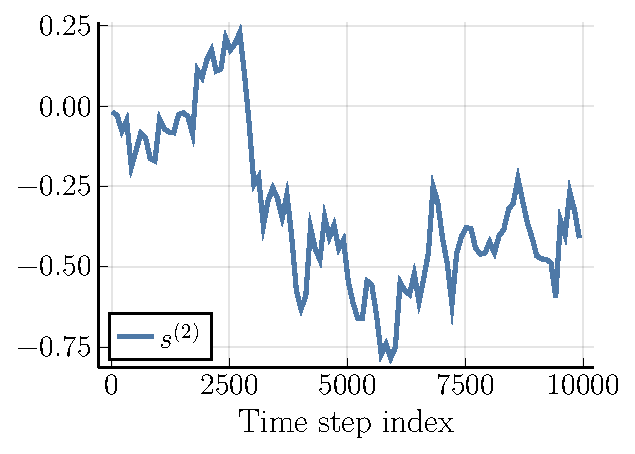
\includegraphics{contents/05-experiments/plots/hgf/04-hierarchical_example_states_1.pdf}
    }
    \caption{Simulated evolution of the layer $s_t^{(2)}$ at time-step index $t$.
    }
    \label{fig:sim:hgf_example_states_1}
  \end{subfigure}
  \hfill
  \begin{subfigure}[t]{0.475\textwidth}
    \centering
    \resizebox{\textwidth}{!}{
        % % Recommended preamble:
% \usetikzlibrary{arrows.meta}
% \usetikzlibrary{backgrounds}
% \usepgfplotslibrary{patchplots}
% \usepgfplotslibrary{fillbetween}
% \pgfplotsset{%
%     layers/standard/.define layer set={%
%         background,axis background,axis grid,axis ticks,axis lines,axis tick labels,pre main,main,axis descriptions,axis foreground%
%     }{
%         grid style={/pgfplots/on layer=axis grid},%
%         tick style={/pgfplots/on layer=axis ticks},%
%         axis line style={/pgfplots/on layer=axis lines},%
%         label style={/pgfplots/on layer=axis descriptions},%
%         legend style={/pgfplots/on layer=axis descriptions},%
%         title style={/pgfplots/on layer=axis descriptions},%
%         colorbar style={/pgfplots/on layer=axis descriptions},%
%         ticklabel style={/pgfplots/on layer=axis tick labels},%
%         axis background@ style={/pgfplots/on layer=axis background},%
%         3d box foreground style={/pgfplots/on layer=axis foreground},%
%     },
% }

\begin{tikzpicture}[/tikz/background rectangle/.style={fill={rgb,1:red,1.0;green,1.0;blue,1.0}, fill opacity={1.0}, draw opacity={1.0}}, show background rectangle]
\begin{axis}[point meta max={nan}, point meta min={nan}, legend cell align={left}, legend columns={1}, title={}, title style={at={{(0.5,1)}}, anchor={south}, font={{\fontsize{18 pt}{23.400000000000002 pt}\selectfont}}, color={rgb,1:red,0.0;green,0.0;blue,0.0}, draw opacity={1.0}, rotate={0.0}, align={center}}, legend style={color={rgb,1:red,0.0;green,0.0;blue,0.0}, draw opacity={1.0}, line width={1}, solid, fill={rgb,1:red,1.0;green,1.0;blue,1.0}, fill opacity={1.0}, text opacity={1.0}, font={{\fontsize{14 pt}{18.2 pt}\selectfont}}, text={rgb,1:red,0.0;green,0.0;blue,0.0}, cells={anchor={center}}, at={(0.98, 0.02)}, anchor={south east}}, axis background/.style={fill={rgb,1:red,1.0;green,1.0;blue,1.0}, opacity={1.0}}, anchor={north west}, xshift={1.0mm}, yshift={-1.0mm}, width={99.6mm}, height={74.2mm}, scaled x ticks={false}, xlabel={Time step index}, x tick style={color={rgb,1:red,0.0;green,0.0;blue,0.0}, opacity={1.0}}, x tick label style={color={rgb,1:red,0.0;green,0.0;blue,0.0}, opacity={1.0}, rotate={0}}, xlabel style={at={(ticklabel cs:0.5)}, anchor=near ticklabel, at={{(ticklabel cs:0.5)}}, anchor={near ticklabel}, font={{\fontsize{16 pt}{20.8 pt}\selectfont}}, color={rgb,1:red,0.0;green,0.0;blue,0.0}, draw opacity={1.0}, rotate={0.0}}, xmajorgrids={true}, xmin={-277.0}, xmax={10217.0}, xticklabels={{$0$,$2500$,$5000$,$7500$,$10000$}}, xtick={{0.0,2500.0,5000.0,7500.0,10000.0}}, xtick align={inside}, xticklabel style={font={{\fontsize{14 pt}{18.2 pt}\selectfont}}, color={rgb,1:red,0.0;green,0.0;blue,0.0}, draw opacity={1.0}, rotate={0.0}}, x grid style={color={rgb,1:red,0.0;green,0.0;blue,0.0}, draw opacity={0.1}, line width={0.5}, solid}, axis x line*={left}, x axis line style={color={rgb,1:red,0.0;green,0.0;blue,0.0}, draw opacity={1.0}, line width={1}, solid}, scaled y ticks={false}, ylabel={}, y tick style={color={rgb,1:red,0.0;green,0.0;blue,0.0}, opacity={1.0}}, y tick label style={color={rgb,1:red,0.0;green,0.0;blue,0.0}, opacity={1.0}, rotate={0}}, ylabel style={at={(ticklabel cs:0.5)}, anchor=near ticklabel, at={{(ticklabel cs:0.5)}}, anchor={near ticklabel}, font={{\fontsize{16 pt}{20.8 pt}\selectfont}}, color={rgb,1:red,0.0;green,0.0;blue,0.0}, draw opacity={1.0}, rotate={0.0}}, ymajorgrids={true}, ymin={-141.9838333878513}, ymax={-1.772464452523593}, yticklabels={{$-125$,$-100$,$-75$,$-50$,$-25$}}, ytick={{-125.0,-100.0,-75.0,-50.0,-25.0}}, ytick align={inside}, yticklabel style={font={{\fontsize{14 pt}{18.2 pt}\selectfont}}, color={rgb,1:red,0.0;green,0.0;blue,0.0}, draw opacity={1.0}, rotate={0.0}}, y grid style={color={rgb,1:red,0.0;green,0.0;blue,0.0}, draw opacity={0.1}, line width={0.5}, solid}, axis y line*={left}, y axis line style={color={rgb,1:red,0.0;green,0.0;blue,0.0}, draw opacity={1.0}, line width={1}, solid}, colorbar={false}]
    \addplot[color={rgb,1:red,0.6902;green,0.4784;blue,0.6314}, name path={1cd19579-c0eb-458b-8ca5-fd6c748a315c}, draw opacity={1.0}, line width={2}, solid]
        table[row sep={\\}]
        {
            \\
            20.0  -5.740710743146092  \\
            120.0  -16.612356409740595  \\
            220.0  -30.214939728674338  \\
            320.0  -27.91277108347563  \\
            420.0  -38.44051445158849  \\
            520.0  -36.37692770870293  \\
            620.0  -28.657499818104238  \\
            720.0  -38.11518859043452  \\
            820.0  -32.23811428629152  \\
            920.0  -28.365027552107573  \\
            1020.0  -30.315432575532842  \\
            1120.0  -46.81987978670828  \\
            1220.0  -46.48164775220454  \\
            1320.0  -33.32503463176701  \\
            1420.0  -35.15999677518617  \\
            1520.0  -35.71038384923469  \\
            1620.0  -40.893894030255126  \\
            1720.0  -39.25486028847835  \\
            1820.0  -50.349916409688475  \\
            1920.0  -51.076761742174455  \\
            2020.0  -58.43102646839949  \\
            2120.0  -69.68685913597517  \\
            2220.0  -63.75342245661089  \\
            2320.0  -73.28334225380378  \\
            2420.0  -76.26316055388325  \\
            2520.0  -115.40808732749156  \\
            2620.0  -110.50279837754361  \\
            2720.0  -95.30321841859855  \\
            2820.0  -92.8887102970675  \\
            2920.0  -110.80200605436752  \\
            3020.0  -119.46090050450783  \\
            3120.0  -126.5299510861929  \\
            3220.0  -121.32351826893401  \\
            3320.0  -125.60844688335281  \\
            3420.0  -133.01014303493668  \\
            3520.0  -138.0155870972288  \\
            3620.0  -129.5261427971083  \\
            3720.0  -122.27921209431543  \\
            3820.0  -120.3164502827986  \\
            3920.0  -113.13666947422665  \\
            4020.0  -113.97850179859742  \\
            4120.0  -125.88220598136336  \\
            4220.0  -126.85244318876003  \\
            4320.0  -118.38418716296158  \\
            4420.0  -111.73366972541768  \\
            4520.0  -119.88683501175005  \\
            4620.0  -92.83742376705094  \\
            4720.0  -91.08626110445321  \\
            4820.0  -86.11334335878445  \\
            4920.0  -78.78128167867484  \\
            5020.0  -77.71717298900397  \\
            5120.0  -76.64967150209743  \\
            5220.0  -72.17253805490954  \\
            5320.0  -80.28208366932938  \\
            5420.0  -72.2365997940903  \\
            5520.0  -54.560365734612056  \\
            5620.0  -57.51253985758529  \\
            5720.0  -70.10017754179482  \\
            5820.0  -68.86698992583172  \\
            5920.0  -78.63023427471254  \\
            6020.0  -84.03854154243193  \\
            6120.0  -79.84480016713425  \\
            6220.0  -79.68251647287082  \\
            6320.0  -88.5079577831925  \\
            6420.0  -93.20288652652177  \\
            6520.0  -85.8003987308885  \\
            6620.0  -80.24422203190426  \\
            6720.0  -76.24930449180981  \\
            6820.0  -64.60282044971704  \\
            6920.0  -64.09617045180755  \\
            7020.0  -68.902151721553  \\
            7120.0  -69.71453784822451  \\
            7220.0  -63.13519862587223  \\
            7320.0  -60.59210851070374  \\
            7420.0  -42.58328751848333  \\
            7520.0  -53.37883529178319  \\
            7620.0  -45.92453440684575  \\
            7720.0  -52.27878794361281  \\
            7820.0  -56.48992201341925  \\
            7920.0  -62.36671362460824  \\
            8020.0  -45.85998106666752  \\
            8120.0  -65.64823797939657  \\
            8220.0  -57.2476583848691  \\
            8320.0  -56.1917153444642  \\
            8420.0  -69.25777132654598  \\
            8520.0  -69.57230538642035  \\
            8620.0  -63.777346085996626  \\
            8720.0  -55.00392627071413  \\
            8820.0  -43.07094713280625  \\
            8920.0  -35.67458728809847  \\
            9020.0  -29.87085725414616  \\
            9120.0  -32.3540078567988  \\
            9220.0  -38.70973810006492  \\
            9320.0  -46.89969966114424  \\
            9420.0  -66.87691878358183  \\
            9520.0  -75.91034514738557  \\
            9620.0  -80.63209074519688  \\
            9720.0  -64.05168590602386  \\
            9820.0  -57.123291475702935  \\
            9920.0  -61.257290866591774  \\
        }
        ;
    \addlegendentry {$s^{(1)}$}
    \addplot[color={rgb,1:red,0.349;green,0.6314;blue,0.3098}, name path={e5a24211-ae00-4d62-9584-c87e53e39175}, only marks, draw opacity={0.5}, line width={0}, solid, mark={*}, mark size={1.5 pt}, mark repeat={1}, mark options={color={rgb,1:red,0.0;green,0.0;blue,0.0}, draw opacity={0.5}, fill={rgb,1:red,0.349;green,0.6314;blue,0.3098}, fill opacity={0.5}, line width={0.0}, rotate={0}, solid}]
        table[row sep={\\}]
        {
            \\
            20.0  -5.742770854791965  \\
            120.0  -17.2895289665243  \\
            220.0  -30.361340286844754  \\
            320.0  -27.704016346290324  \\
            420.0  -38.302895249889275  \\
            520.0  -36.677634111622766  \\
            620.0  -28.644058786972053  \\
            720.0  -38.141224988304835  \\
            820.0  -32.580190010420054  \\
            920.0  -28.63268053136293  \\
            1020.0  -30.721186493666398  \\
            1120.0  -46.40489702462974  \\
            1220.0  -46.99337372808301  \\
            1320.0  -33.05856626021657  \\
            1420.0  -35.452662992160825  \\
            1520.0  -36.21238580493504  \\
            1620.0  -41.31875559694605  \\
            1720.0  -39.078578990395606  \\
            1820.0  -50.63439290330427  \\
            1920.0  -51.086983322520624  \\
            2020.0  -58.361111038157105  \\
            2120.0  -70.00720496159775  \\
            2220.0  -63.690482907628954  \\
            2320.0  -73.79779244027957  \\
            2420.0  -76.34354013802468  \\
            2520.0  -115.61342839739346  \\
            2620.0  -110.41669342141986  \\
            2720.0  -95.34989752090296  \\
            2820.0  -93.12028579372817  \\
            2920.0  -110.66583791070892  \\
            3020.0  -119.5096387013258  \\
            3120.0  -126.30117533529366  \\
            3220.0  -121.18310402678331  \\
            3320.0  -125.40914331079675  \\
            3420.0  -133.06326899710115  \\
            3520.0  -137.96946127226911  \\
            3620.0  -129.44258604526055  \\
            3720.0  -121.71322100365353  \\
            3820.0  -120.71921825157227  \\
            3920.0  -113.22379873129485  \\
            4020.0  -113.62188174125336  \\
            4120.0  -126.46820918013178  \\
            4220.0  -126.93585357927385  \\
            4320.0  -118.35283789490236  \\
            4420.0  -111.29335819176698  \\
            4520.0  -119.90163627876177  \\
            4620.0  -92.43253286840418  \\
            4720.0  -91.07210968551689  \\
            4820.0  -85.68851702146705  \\
            4920.0  -79.15102338448396  \\
            5020.0  -77.88424675719315  \\
            5120.0  -76.59743529190374  \\
            5220.0  -71.90848144492746  \\
            5320.0  -80.73391791260532  \\
            5420.0  -71.95886687283739  \\
            5520.0  -54.5832402306863  \\
            5620.0  -57.31268120942707  \\
            5720.0  -70.15880529961798  \\
            5820.0  -68.9112088642401  \\
            5920.0  -78.71551797595836  \\
            6020.0  -84.35387311303546  \\
            6120.0  -79.81893822708403  \\
            6220.0  -78.94632055008643  \\
            6320.0  -88.45872943103531  \\
            6420.0  -93.03864950480617  \\
            6520.0  -85.69920440386407  \\
            6620.0  -80.17649312342434  \\
            6720.0  -76.37011098376705  \\
            6820.0  -64.7659676967172  \\
            6920.0  -64.25657293334554  \\
            7020.0  -68.79682725587386  \\
            7120.0  -69.47587744497314  \\
            7220.0  -63.04387302173695  \\
            7320.0  -60.89407673695217  \\
            7420.0  -42.55153056554662  \\
            7520.0  -53.63647523858669  \\
            7620.0  -46.130856025096804  \\
            7720.0  -52.67119451869334  \\
            7820.0  -56.92936871748146  \\
            7920.0  -62.58934108392828  \\
            8020.0  -45.71437237839573  \\
            8120.0  -65.68806834595546  \\
            8220.0  -57.24014878403126  \\
            8320.0  -56.018298242955666  \\
            8420.0  -69.38202679895872  \\
            8520.0  -69.66311027098386  \\
            8620.0  -63.57080652991492  \\
            8720.0  -54.875127370085764  \\
            8820.0  -42.95452380221737  \\
            8920.0  -35.910045616945354  \\
            9020.0  -29.40618005008118  \\
            9120.0  -32.42537960864664  \\
            9220.0  -38.7585851696836  \\
            9320.0  -47.067333417680416  \\
            9420.0  -66.78553207005805  \\
            9520.0  -76.07856038466359  \\
            9620.0  -80.69759584687029  \\
            9720.0  -63.87501906109672  \\
            9820.0  -57.12550346293002  \\
            9920.0  -61.13180115333624  \\
        }
        ;
    \addlegendentry {$y$}
\end{axis}
\end{tikzpicture}

        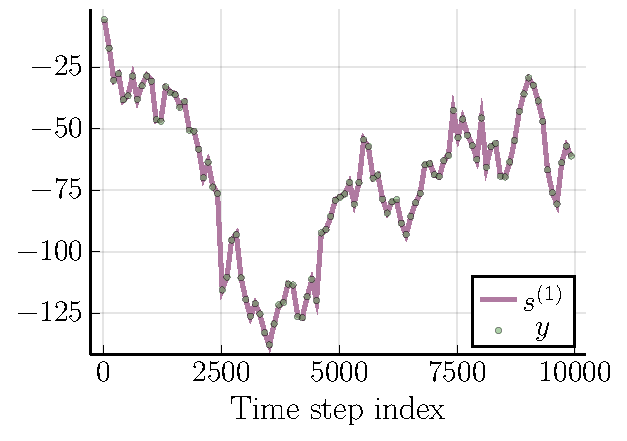
\includegraphics{contents/05-experiments/plots/hgf/04-hierarchical_example_states_2.pdf}
    }
    \caption{Simulated evolution of the layer $s_t^{(1)}$ and measurements $y$ at time-step index $t$.}
    \label{fig:sim:hgf_example_states_2}
  \end{subfigure}
  \caption{
    Simulated evolution of the 2-layer \ac{hgf} model \eqref{eq:sim:hgf_model} for $10,000$ synthetically generated 1-dimensional observations with link function $f(s) = exp(\kappa s + \zeta)$, where $\kappa = 1$ and $\zeta = 0$.
    The noise component $\Sigma$ is set to be $10^{-4}$, the noise component $\Omega$ is set to be
    $0.0625$.
  }
  \label{fig:sim:hgf_example_states}
\end{figure}

\subsection{The probabilistic model and the inference specification}
\begin{figure*}
  \begin{adjustbox}{minipage=\textwidth,margin=0pt \smallskipamount,center}
    \jlinputlisting[label={lst:sim:hgf_model_specification}, caption={An example of specification of the probabilistic 2-layer \ac{hgf} model~\eqref{eq:sim:hgf_model}.
        },captionpos=b]{contents/05-experiments/code/04-hgf-model.jl}
  \end{adjustbox}
\end{figure*}
Listing~\ref{lst:sim:hgf_model_specification} presents an example of the specification of the probabilistic 2-layer \ac{hgf} model~\eqref{eq:sim:hgf_model} using the RxInfer framework.
As part of the inference specification, we define extra factorization constraints for the
variational family of distributions $Q_{B}$ with the \jlinl{@constraints} macro.
The extra constraints assume that states $\bm{z}$, $\bm{x}$, and the precision of the
measurement noise are jointly independent.
\begin{figure*}
  \begin{adjustbox}{minipage=\textwidth,margin=0pt \smallskipamount,center}
    \jlinputlisting[label={lst:sim:hgf_constraints}, caption={Extra factorization constraints for the variational family of distributions $Q_{B}$ for the probabilistic model of the 2-layer \ac{hgf} system defined in Listing~\eqref{lst:sim:hgf_model_specification}.
        },captionpos=b]{contents/05-experiments/code/04-hgf-constraints.jl}
  \end{adjustbox}
\end{figure*}
In order to execute the inference procedure, we use the \jlinl{rxinference()} function, which
supports streaming datasets and continual inference.
The \jlinl{rxinference()} function subscribes to a data source and performs continual
inference as soon as new measurements become available.
In between measurements, while idle, the inference engine can perform additional \ac{vmp} iterations to
increase the accuracy of the estimated posteriors.
We use the \jlinl{@autoupdates} macro to specify how to update the prior information at time
step index $t$ using the posterior information from time step index $t - 1$.
Figure~\ref{fig:sim:hgf_inference_states} shows an example of the inference task and inferred
posterior distributions over states with their corresponding uncertainties.
For this type of model, the full model and inference specifications require around 40 lines of
code  (\hyperlink{experiments:userfriendliness}{\emph{User-friendliness}}).
\begin{figure*}
  \begin{adjustbox}{minipage=\textwidth,margin=0pt \smallskipamount,center}
    \jlinputlisting[label={lst:sim:hgf_inference}, caption={An example of the inference execution for the probabilistic model of the 2-layer \ac{hgf} model defined in Listing~\eqref{lst:sim:hgf_model_specification} with constraints defined in Listing~\ref{lst:sim:hgf_constraints}.
          The \jlinl{@autoupdates} macro specifies how to update the prior information at time step index $t$
          by using the posterior information from time step index $t - 1$.
        },captionpos=b]{contents/05-experiments/code/04-hgf-inference.jl}
  \end{adjustbox}
\end{figure*}

\begin{figure}
  \centering
  \begin{subfigure}[t]{0.315\textwidth}
    \centering
    \resizebox{\textwidth}{!}{
        % % Recommended preamble:
% \usetikzlibrary{arrows.meta}
% \usetikzlibrary{backgrounds}
% \usepgfplotslibrary{patchplots}
% \usepgfplotslibrary{fillbetween}
% \pgfplotsset{%
%     layers/standard/.define layer set={%
%         background,axis background,axis grid,axis ticks,axis lines,axis tick labels,pre main,main,axis descriptions,axis foreground%
%     }{
%         grid style={/pgfplots/on layer=axis grid},%
%         tick style={/pgfplots/on layer=axis ticks},%
%         axis line style={/pgfplots/on layer=axis lines},%
%         label style={/pgfplots/on layer=axis descriptions},%
%         legend style={/pgfplots/on layer=axis descriptions},%
%         title style={/pgfplots/on layer=axis descriptions},%
%         colorbar style={/pgfplots/on layer=axis descriptions},%
%         ticklabel style={/pgfplots/on layer=axis tick labels},%
%         axis background@ style={/pgfplots/on layer=axis background},%
%         3d box foreground style={/pgfplots/on layer=axis foreground},%
%     },
% }

\begin{tikzpicture}[/tikz/background rectangle/.style={fill={rgb,1:red,1.0;green,1.0;blue,1.0}, fill opacity={1.0}, draw opacity={1.0}}, show background rectangle]
\begin{axis}[point meta max={nan}, point meta min={nan}, legend cell align={left}, legend columns={1}, title={}, title style={at={{(0.5,1)}}, anchor={south}, font={{\fontsize{18 pt}{23.400000000000002 pt}\selectfont}}, color={rgb,1:red,0.0;green,0.0;blue,0.0}, draw opacity={1.0}, rotate={0.0}, align={center}}, legend style={color={rgb,1:red,0.0;green,0.0;blue,0.0}, draw opacity={1.0}, line width={1}, solid, fill={rgb,1:red,1.0;green,1.0;blue,1.0}, fill opacity={1.0}, text opacity={1.0}, font={{\fontsize{14 pt}{18.2 pt}\selectfont}}, text={rgb,1:red,0.0;green,0.0;blue,0.0}, cells={anchor={center}}, at={(0.02, 0.02)}, anchor={south west}}, axis background/.style={fill={rgb,1:red,1.0;green,1.0;blue,1.0}, opacity={1.0}}, anchor={north west}, xshift={1.0mm}, yshift={-1.0mm}, width={99.6mm}, height={74.2mm}, scaled x ticks={false}, xlabel={Time step index}, x tick style={color={rgb,1:red,0.0;green,0.0;blue,0.0}, opacity={1.0}}, x tick label style={color={rgb,1:red,0.0;green,0.0;blue,0.0}, opacity={1.0}, rotate={0}}, xlabel style={at={(ticklabel cs:0.5)}, anchor=near ticklabel, at={{(ticklabel cs:0.5)}}, anchor={near ticklabel}, font={{\fontsize{16 pt}{20.8 pt}\selectfont}}, color={rgb,1:red,0.0;green,0.0;blue,0.0}, draw opacity={1.0}, rotate={0.0}}, xmajorgrids={true}, xmin={-277.0}, xmax={10217.0}, xticklabels={{$0$,$2500$,$5000$,$7500$,$10000$}}, xtick={{0.0,2500.0,5000.0,7500.0,10000.0}}, xtick align={inside}, xticklabel style={font={{\fontsize{14 pt}{18.2 pt}\selectfont}}, color={rgb,1:red,0.0;green,0.0;blue,0.0}, draw opacity={1.0}, rotate={0.0}}, x grid style={color={rgb,1:red,0.0;green,0.0;blue,0.0}, draw opacity={0.1}, line width={0.5}, solid}, axis x line*={left}, x axis line style={color={rgb,1:red,0.0;green,0.0;blue,0.0}, draw opacity={1.0}, line width={1}, solid}, scaled y ticks={false}, ylabel={}, y tick style={color={rgb,1:red,0.0;green,0.0;blue,0.0}, opacity={1.0}}, y tick label style={color={rgb,1:red,0.0;green,0.0;blue,0.0}, opacity={1.0}, rotate={0}}, ylabel style={at={(ticklabel cs:0.5)}, anchor=near ticklabel, at={{(ticklabel cs:0.5)}}, anchor={near ticklabel}, font={{\fontsize{16 pt}{20.8 pt}\selectfont}}, color={rgb,1:red,0.0;green,0.0;blue,0.0}, draw opacity={1.0}, rotate={0.0}}, ymajorgrids={true}, ymin={-1.3490315915537232}, ymax={0.9652708372225225}, yticklabels={{$-1.0$,$-0.5$,$0.0$,$0.5$}}, ytick={{-1.0,-0.5,0.0,0.5}}, ytick align={inside}, yticklabel style={font={{\fontsize{14 pt}{18.2 pt}\selectfont}}, color={rgb,1:red,0.0;green,0.0;blue,0.0}, draw opacity={1.0}, rotate={0.0}}, y grid style={color={rgb,1:red,0.0;green,0.0;blue,0.0}, draw opacity={0.1}, line width={0.5}, solid}, axis y line*={left}, y axis line style={color={rgb,1:red,0.0;green,0.0;blue,0.0}, draw opacity={1.0}, line width={1}, solid}, colorbar={false}]
    \addplot[color={rgb,1:red,0.3059;green,0.4745;blue,0.6549}, name path={d51c1e62-caba-4845-b716-1b868951d96a}, draw opacity={1.0}, line width={2}, solid]
        table[row sep={\\}]
        {
            \\
            20.0  -0.017714363408717806  \\
            120.0  -0.03031981561889148  \\
            220.0  -0.07800584656637763  \\
            320.0  -0.04519637569374746  \\
            420.0  -0.1895501683882646  \\
            520.0  -0.13913084966651065  \\
            620.0  -0.08436277750576925  \\
            720.0  -0.09797280644765398  \\
            820.0  -0.16273269716836208  \\
            920.0  -0.17093628238947195  \\
            1020.0  -0.040487855729603374  \\
            1120.0  -0.07146781786101417  \\
            1220.0  -0.08137131947457325  \\
            1320.0  -0.08331049795742647  \\
            1420.0  -0.027082052108420053  \\
            1520.0  -0.020970920788733  \\
            1620.0  -0.03252297100148165  \\
            1720.0  -0.086440896874568  \\
            1820.0  0.11213137879371679  \\
            1920.0  0.08815498954468355  \\
            2020.0  0.14345061360549682  \\
            2120.0  0.1738527859331274  \\
            2220.0  0.10879263777994755  \\
            2320.0  0.11578974595019646  \\
            2420.0  0.21189099806617784  \\
            2520.0  0.17471603913173184  \\
            2620.0  0.1940969962494026  \\
            2720.0  0.22809756877159054  \\
            2820.0  0.098922235335671  \\
            2920.0  -0.05678279872933818  \\
            3020.0  -0.24475581600360727  \\
            3120.0  -0.2208990189017549  \\
            3220.0  -0.3717816414372628  \\
            3320.0  -0.29437667409377277  \\
            3420.0  -0.2547804879820489  \\
            3520.0  -0.28768061676987144  \\
            3620.0  -0.34658664027291913  \\
            3720.0  -0.27476348762155245  \\
            3820.0  -0.4045932962998529  \\
            3920.0  -0.5740173883824468  \\
            4020.0  -0.6308775952582358  \\
            4120.0  -0.5908993033096395  \\
            4220.0  -0.37771297964588096  \\
            4320.0  -0.44430788734534865  \\
            4420.0  -0.4782393466750803  \\
            4520.0  -0.3455428357818275  \\
            4620.0  -0.40794146878337273  \\
            4720.0  -0.3702044711798191  \\
            4820.0  -0.4436461419290132  \\
            4920.0  -0.4165204606850431  \\
            5020.0  -0.5447681612031563  \\
            5120.0  -0.6114824088606563  \\
            5220.0  -0.659415522369523  \\
            5320.0  -0.6597703176064015  \\
            5420.0  -0.5445400917547797  \\
            5520.0  -0.5570346671260175  \\
            5620.0  -0.6500542929659792  \\
            5720.0  -0.7725905542524371  \\
            5820.0  -0.7411114853817794  \\
            5920.0  -0.7838892608921646  \\
            6020.0  -0.7505524729662401  \\
            6120.0  -0.5483448523563014  \\
            6220.0  -0.5749361962229627  \\
            6320.0  -0.5861312430977571  \\
            6420.0  -0.522411917093636  \\
            6520.0  -0.6088670719475303  \\
            6620.0  -0.536545727208839  \\
            6720.0  -0.45758892375242727  \\
            6820.0  -0.25089382283913253  \\
            6920.0  -0.3005925555325212  \\
            7020.0  -0.41158857861972004  \\
            7120.0  -0.4895960418461227  \\
            7220.0  -0.6171390716217825  \\
            7320.0  -0.4585750650805316  \\
            7420.0  -0.4067140042212498  \\
            7520.0  -0.3789104419364966  \\
            7620.0  -0.3803157427107729  \\
            7720.0  -0.4412833610534849  \\
            7820.0  -0.46073681965898683  \\
            7920.0  -0.4574115909860456  \\
            8020.0  -0.42286771458994826  \\
            8120.0  -0.45621762002053007  \\
            8220.0  -0.4040413533620254  \\
            8320.0  -0.3835930733413548  \\
            8420.0  -0.32131668900844806  \\
            8520.0  -0.30230029914527945  \\
            8620.0  -0.2258579882256835  \\
            8720.0  -0.29642084043101585  \\
            8820.0  -0.36362618213865744  \\
            8920.0  -0.41054919683347724  \\
            9020.0  -0.4665089007710655  \\
            9120.0  -0.47557076349016303  \\
            9220.0  -0.4773433112965115  \\
            9320.0  -0.4877681450542384  \\
            9420.0  -0.5946407299602552  \\
            9520.0  -0.3562315069345538  \\
            9620.0  -0.40078300804689077  \\
            9720.0  -0.2682871133517609  \\
            9820.0  -0.32543610543080337  \\
            9920.0  -0.4094592664079163  \\
        }
        ;
    \addlegendentry {$z$}
    \addplot+[line width={0}, draw opacity={0}, fill={rgb,1:red,0.949;green,0.5569;blue,0.1686}, fill opacity={0.5}, mark={none}, forget plot]
        coordinates {
            (20,-0.13662375932419052)
            (120,-0.08886163728899887)
            (220,-0.14532020372812837)
            (320,-0.1298301037676746)
            (420,-0.16073027810209967)
            (520,-0.22531707024971168)
            (620,-0.22463414646110305)
            (720,-0.16055510594810044)
            (820,-0.2082474142725524)
            (920,-0.09801239289530621)
            (1020,-0.1548343174645875)
            (1120,-0.1536825667772715)
            (1220,-0.15504666702264916)
            (1320,-0.253556007033205)
            (1420,-0.21654166214854667)
            (1520,-0.18474593316153468)
            (1620,-0.14357873694384196)
            (1720,-0.2245407895447362)
            (1820,-0.10482461639257336)
            (1920,-0.1047704235413623)
            (2020,0.04976050317033892)
            (2120,0.2515122346886318)
            (2220,0.24567170175880207)
            (2320,0.23733979781810458)
            (2420,0.27905915254611335)
            (2520,0.3261128878563081)
            (2620,0.27619739660074205)
            (2720,0.1473221850819774)
            (2820,0.13658033913580653)
            (2920,0.033642292746779524)
            (3020,0.0015441871197079899)
            (3120,-0.041095223801829596)
            (3220,-0.13107923379443104)
            (3320,-0.31664686628296423)
            (3420,-0.26664194097315574)
            (3520,-0.27881112354389187)
            (3620,-0.22102855323490248)
            (3720,-0.21538657546444398)
            (3820,-0.3088094126125226)
            (3920,-0.39636412176160507)
            (4020,-0.5666901894831511)
            (4120,-0.6607849619168624)
            (4220,-0.6419621489555639)
            (4320,-0.6787529488492452)
            (4420,-0.6666055579824426)
            (4520,-0.5900007009787386)
            (4620,-0.4084347981814856)
            (4720,-0.4542304854948032)
            (4820,-0.49506352030839496)
            (4920,-0.5049067535967147)
            (5020,-0.5674875597343266)
            (5120,-0.5047431144350949)
            (5220,-0.6471567945044792)
            (5320,-0.6331651684360192)
            (5420,-0.7259275210985237)
            (5520,-0.5441385573896556)
            (5620,-0.67133481569063)
            (5720,-0.8072897878537496)
            (5820,-0.7813677422223922)
            (5920,-0.8749179279411304)
            (6020,-0.9194859533097043)
            (6120,-0.8321626117316878)
            (6220,-0.7616510956443793)
            (6320,-0.7838327822803708)
            (6420,-0.696911052226448)
            (6520,-0.6332709009471673)
            (6620,-0.6610295771067768)
            (6720,-0.6958017669258763)
            (6820,-0.6693676731879301)
            (6920,-0.5881376925001676)
            (7020,-0.586927001386452)
            (7120,-0.44110609711291665)
            (7220,-0.5393909800744985)
            (7320,-0.5163716162930038)
            (7420,-0.43667419933802687)
            (7520,-0.3576380865815387)
            (7620,-0.3777665725269111)
            (7720,-0.3200522118331461)
            (7820,-0.45373878852521643)
            (7920,-0.5205245689717846)
            (8020,-0.5416210399937935)
            (8120,-0.4784817187788301)
            (8220,-0.5796717839189898)
            (8320,-0.5028515547207706)
            (8420,-0.5304537038775345)
            (8520,-0.4611195664628924)
            (8620,-0.3891581270266481)
            (8720,-0.4064170472609906)
            (8820,-0.36199456282981524)
            (8920,-0.43904056514124623)
            (9020,-0.5739918897148085)
            (9120,-0.5082305120129171)
            (9220,-0.5017836966510122)
            (9320,-0.5455396535718962)
            (9420,-0.5398734591059908)
            (9520,-0.5835185753232336)
            (9620,-0.5477931834993403)
            (9720,-0.43059695622542377)
            (9820,-0.421128873291206)
            (9920,-0.39148061856177785)
            (9920,-0.7456446884100113)
            (9820,-0.7704186080361717)
            (9720,-0.7772885535686217)
            (9620,-0.9057661646181736)
            (9520,-0.9406010434578399)
            (9420,-0.8947169567967596)
            (9320,-0.906433138034549)
            (9220,-0.8598143697901808)
            (9120,-0.8528720615972795)
            (9020,-0.9441352219464987)
            (8920,-0.8017159153823983)
            (8820,-0.7162670506986395)
            (8720,-0.7651696959901244)
            (8620,-0.7346348789321607)
            (8520,-0.8182066134494568)
            (8420,-0.8930120885911009)
            (8320,-0.8664876582103849)
            (8220,-0.9477013364057187)
            (8120,-0.831876422532539)
            (8020,-0.900752455298987)
            (7920,-0.886565046209526)
            (7820,-0.8231328584661031)
            (7720,-0.6711720844390547)
            (7620,-0.7300318828836065)
            (7520,-0.7032692488108301)
            (7420,-0.7855882281647852)
            (7320,-0.8717824963741834)
            (7220,-0.9032536898002886)
            (7120,-0.7866726022243336)
            (7020,-0.9349100193617856)
            (6920,-0.940880143715396)
            (6820,-1.022836834411095)
            (6720,-1.055678563527897)
            (6620,-1.0231622596322731)
            (6520,-0.9798428974437905)
            (6420,-1.0514713505212852)
            (6320,-1.14255473146047)
            (6220,-1.1151601440963312)
            (6120,-1.1826066804462672)
            (6020,-1.2835324662109993)
            (5920,-1.2462800767713058)
            (5820,-1.1421934251175965)
            (5720,-1.1778505032550095)
            (5620,-1.036831286314177)
            (5520,-0.8848169462770873)
            (5420,-1.0857957105236804)
            (5320,-0.9899735495240076)
            (5220,-1.014328948461368)
            (5120,-0.8609400389327935)
            (5020,-0.9288527324099007)
            (4920,-0.8652835510168209)
            (4820,-0.8559589368055882)
            (4720,-0.8105650695033468)
            (4620,-0.7455690753289126)
            (4520,-0.9441677434270105)
            (4420,-1.0268572077540687)
            (4320,-1.0384290809627952)
            (4220,-0.9988161884232748)
            (4120,-1.028293368744019)
            (4020,-0.9414039847467325)
            (3920,-0.7651382909318094)
            (3820,-0.6790394343765801)
            (3720,-0.5708025078160731)
            (3620,-0.5675979968833056)
            (3520,-0.635150235619758)
            (3420,-0.6235733245531393)
            (3320,-0.6882133444285339)
            (3220,-0.4962151044021869)
            (3120,-0.40505900278031964)
            (3020,-0.36238825221959314)
            (2920,-0.3419676754490263)
            (2820,-0.22847229476393843)
            (2720,-0.22148670564673992)
            (2620,-0.08193867318792081)
            (2520,-0.021890249726240596)
            (2420,-0.07778642913652112)
            (2320,-0.1220592201329592)
            (2220,-0.10036535193888149)
            (2120,-0.08304063494770497)
            (2020,-0.29785124369902655)
            (1920,-0.4615295835235142)
            (1820,-0.45554342860883157)
            (1720,-0.58492488340902)
            (1620,-0.49717608698199167)
            (1520,-0.5439033419097368)
            (1420,-0.5685240286539183)
            (1320,-0.6157490425872044)
            (1220,-0.5103515156855458)
            (1120,-0.5056990059839654)
            (1020,-0.5066645414974495)
            (920,-0.44463216338919237)
            (820,-0.565481109845074)
            (720,-0.5110597648173717)
            (620,-0.5815661916181503)
            (520,-0.5948796319236886)
            (420,-0.5235197108265293)
            (320,-0.49211744830344095)
            (220,-0.5299467794084954)
            (120,-0.5266581597599148)
            (20,-1.1730192305281797)
            (20,-0.13662375932419052)
        }
        ;
    \addplot+[line width={0}, draw opacity={0}, fill={rgb,1:red,0.949;green,0.5569;blue,0.1686}, fill opacity={0.5}, mark={none}, forget plot]
        coordinates {
            (20,-0.13662375932419052)
            (120,-0.08886163728899887)
            (220,-0.14532020372812837)
            (320,-0.1298301037676746)
            (420,-0.16073027810209967)
            (520,-0.22531707024971168)
            (620,-0.22463414646110305)
            (720,-0.16055510594810044)
            (820,-0.2082474142725524)
            (920,-0.09801239289530621)
            (1020,-0.1548343174645875)
            (1120,-0.1536825667772715)
            (1220,-0.15504666702264916)
            (1320,-0.253556007033205)
            (1420,-0.21654166214854667)
            (1520,-0.18474593316153468)
            (1620,-0.14357873694384196)
            (1720,-0.2245407895447362)
            (1820,-0.10482461639257336)
            (1920,-0.1047704235413623)
            (2020,0.04976050317033892)
            (2120,0.2515122346886318)
            (2220,0.24567170175880207)
            (2320,0.23733979781810458)
            (2420,0.27905915254611335)
            (2520,0.3261128878563081)
            (2620,0.27619739660074205)
            (2720,0.1473221850819774)
            (2820,0.13658033913580653)
            (2920,0.033642292746779524)
            (3020,0.0015441871197079899)
            (3120,-0.041095223801829596)
            (3220,-0.13107923379443104)
            (3320,-0.31664686628296423)
            (3420,-0.26664194097315574)
            (3520,-0.27881112354389187)
            (3620,-0.22102855323490248)
            (3720,-0.21538657546444398)
            (3820,-0.3088094126125226)
            (3920,-0.39636412176160507)
            (4020,-0.5666901894831511)
            (4120,-0.6607849619168624)
            (4220,-0.6419621489555639)
            (4320,-0.6787529488492452)
            (4420,-0.6666055579824426)
            (4520,-0.5900007009787386)
            (4620,-0.4084347981814856)
            (4720,-0.4542304854948032)
            (4820,-0.49506352030839496)
            (4920,-0.5049067535967147)
            (5020,-0.5674875597343266)
            (5120,-0.5047431144350949)
            (5220,-0.6471567945044792)
            (5320,-0.6331651684360192)
            (5420,-0.7259275210985237)
            (5520,-0.5441385573896556)
            (5620,-0.67133481569063)
            (5720,-0.8072897878537496)
            (5820,-0.7813677422223922)
            (5920,-0.8749179279411304)
            (6020,-0.9194859533097043)
            (6120,-0.8321626117316878)
            (6220,-0.7616510956443793)
            (6320,-0.7838327822803708)
            (6420,-0.696911052226448)
            (6520,-0.6332709009471673)
            (6620,-0.6610295771067768)
            (6720,-0.6958017669258763)
            (6820,-0.6693676731879301)
            (6920,-0.5881376925001676)
            (7020,-0.586927001386452)
            (7120,-0.44110609711291665)
            (7220,-0.5393909800744985)
            (7320,-0.5163716162930038)
            (7420,-0.43667419933802687)
            (7520,-0.3576380865815387)
            (7620,-0.3777665725269111)
            (7720,-0.3200522118331461)
            (7820,-0.45373878852521643)
            (7920,-0.5205245689717846)
            (8020,-0.5416210399937935)
            (8120,-0.4784817187788301)
            (8220,-0.5796717839189898)
            (8320,-0.5028515547207706)
            (8420,-0.5304537038775345)
            (8520,-0.4611195664628924)
            (8620,-0.3891581270266481)
            (8720,-0.4064170472609906)
            (8820,-0.36199456282981524)
            (8920,-0.43904056514124623)
            (9020,-0.5739918897148085)
            (9120,-0.5082305120129171)
            (9220,-0.5017836966510122)
            (9320,-0.5455396535718962)
            (9420,-0.5398734591059908)
            (9520,-0.5835185753232336)
            (9620,-0.5477931834993403)
            (9720,-0.43059695622542377)
            (9820,-0.421128873291206)
            (9920,-0.39148061856177785)
            (9920,-0.037316548713544395)
            (9820,-0.07183913854624036)
            (9720,-0.08390535888222583)
            (9620,-0.18982020238050684)
            (9520,-0.22643610718862728)
            (9420,-0.1850299614152221)
            (9320,-0.18464616910924336)
            (9220,-0.14375302351184366)
            (9120,-0.1635889624285548)
            (9020,-0.20384855748311842)
            (8920,-0.07636521490009412)
            (8820,-0.007722074960990921)
            (8720,-0.04766439853185683)
            (8620,-0.04368137512113546)
            (8520,-0.10403251947632813)
            (8420,-0.16789531916396816)
            (8320,-0.1392154512311563)
            (8220,-0.21164223143226085)
            (8120,-0.12508701502512126)
            (8020,-0.18248962468860003)
            (7920,-0.1544840917340431)
            (7820,-0.08434471858432974)
            (7720,0.031067660772762518)
            (7620,-0.025501262170215644)
            (7520,-0.012006924352247206)
            (7420,-0.08776017051126855)
            (7320,-0.16096073621182416)
            (7220,-0.17552827034870833)
            (7120,-0.0955395920014997)
            (7020,-0.23894398341111844)
            (6920,-0.2353952412849391)
            (6820,-0.3158985119647652)
            (6720,-0.33592497032385554)
            (6620,-0.29889689458128055)
            (6520,-0.28669890445054413)
            (6420,-0.34235075393161074)
            (6320,-0.4251108331002715)
            (6220,-0.4081420471924274)
            (6120,-0.48171854301710854)
            (6020,-0.5554394404084093)
            (5920,-0.5035557791109551)
            (5820,-0.420542059327188)
            (5720,-0.4367290724524898)
            (5620,-0.3058383450670831)
            (5520,-0.20346016850222381)
            (5420,-0.36605933167336685)
            (5320,-0.27635678734803076)
            (5220,-0.27998464054759037)
            (5120,-0.14854618993739627)
            (5020,-0.20612238705875247)
            (4920,-0.14452995617660847)
            (4820,-0.13416810381120164)
            (4720,-0.09789590148625954)
            (4620,-0.07130052103405865)
            (4520,-0.23583365853046667)
            (4420,-0.3063539082108163)
            (4320,-0.3190768167356952)
            (4220,-0.28510810948785303)
            (4120,-0.29327655508970574)
            (4020,-0.1919763942195697)
            (3920,-0.02758995259140068)
            (3820,0.06142060915153491)
            (3720,0.14002935688718512)
            (3620,0.1255408904135006)
            (3520,0.07752798853197435)
            (3420,0.09028944260682781)
            (3320,0.05491961186260541)
            (3220,0.23405663681332484)
            (3120,0.3228685551766604)
            (3020,0.36547662645900914)
            (2920,0.4092522609425854)
            (2820,0.5016329730355515)
            (2720,0.5161310758106947)
            (2620,0.6343334663894049)
            (2520,0.6741160254388567)
            (2420,0.6359047342287478)
            (2320,0.5967388157691683)
            (2220,0.5917087554564856)
            (2120,0.5860651043249686)
            (2020,0.3973722500397044)
            (1920,0.2519887364407896)
            (1820,0.24589419582368488)
            (1720,0.13584330431954764)
            (1620,0.21001861309430772)
            (1520,0.17441147558666745)
            (1420,0.1354407043568249)
            (1320,0.10863702852079438)
            (1220,0.20025818164024753)
            (1120,0.1983338724294224)
            (1020,0.1969959065682745)
            (920,0.24860737759857993)
            (820,0.14898628129996921)
            (720,0.1899495529211708)
            (620,0.13229789869594413)
            (520,0.14424549142426532)
            (420,0.20205915462232987)
            (320,0.23245724076809174)
            (220,0.2393063719522387)
            (120,0.34893488518191706)
            (20,0.8997717118797985)
            (20,-0.13662375932419052)
        }
        ;
    \addplot[color={rgb,1:red,0.949;green,0.5569;blue,0.1686}, name path={88fc2b49-5bdc-4196-98e1-3b1c0545778e}, legend image code/.code={{
    \draw[fill={rgb,1:red,0.949;green,0.5569;blue,0.1686}, fill opacity={0.5}] (0cm,-0.1cm) rectangle (0.6cm,0.1cm);
    }}, draw opacity={1.0}, line width={2}, solid]
        table[row sep={\\}]
        {
            \\
            20.0  -0.13662375932419052  \\
            120.0  -0.08886163728899887  \\
            220.0  -0.14532020372812837  \\
            320.0  -0.1298301037676746  \\
            420.0  -0.16073027810209967  \\
            520.0  -0.22531707024971168  \\
            620.0  -0.22463414646110305  \\
            720.0  -0.16055510594810044  \\
            820.0  -0.2082474142725524  \\
            920.0  -0.09801239289530621  \\
            1020.0  -0.1548343174645875  \\
            1120.0  -0.1536825667772715  \\
            1220.0  -0.15504666702264916  \\
            1320.0  -0.253556007033205  \\
            1420.0  -0.21654166214854667  \\
            1520.0  -0.18474593316153468  \\
            1620.0  -0.14357873694384196  \\
            1720.0  -0.2245407895447362  \\
            1820.0  -0.10482461639257336  \\
            1920.0  -0.1047704235413623  \\
            2020.0  0.04976050317033892  \\
            2120.0  0.2515122346886318  \\
            2220.0  0.24567170175880207  \\
            2320.0  0.23733979781810458  \\
            2420.0  0.27905915254611335  \\
            2520.0  0.3261128878563081  \\
            2620.0  0.27619739660074205  \\
            2720.0  0.1473221850819774  \\
            2820.0  0.13658033913580653  \\
            2920.0  0.033642292746779524  \\
            3020.0  0.0015441871197079899  \\
            3120.0  -0.041095223801829596  \\
            3220.0  -0.13107923379443104  \\
            3320.0  -0.31664686628296423  \\
            3420.0  -0.26664194097315574  \\
            3520.0  -0.27881112354389187  \\
            3620.0  -0.22102855323490248  \\
            3720.0  -0.21538657546444398  \\
            3820.0  -0.3088094126125226  \\
            3920.0  -0.39636412176160507  \\
            4020.0  -0.5666901894831511  \\
            4120.0  -0.6607849619168624  \\
            4220.0  -0.6419621489555639  \\
            4320.0  -0.6787529488492452  \\
            4420.0  -0.6666055579824426  \\
            4520.0  -0.5900007009787386  \\
            4620.0  -0.4084347981814856  \\
            4720.0  -0.4542304854948032  \\
            4820.0  -0.49506352030839496  \\
            4920.0  -0.5049067535967147  \\
            5020.0  -0.5674875597343266  \\
            5120.0  -0.5047431144350949  \\
            5220.0  -0.6471567945044792  \\
            5320.0  -0.6331651684360192  \\
            5420.0  -0.7259275210985237  \\
            5520.0  -0.5441385573896556  \\
            5620.0  -0.67133481569063  \\
            5720.0  -0.8072897878537496  \\
            5820.0  -0.7813677422223922  \\
            5920.0  -0.8749179279411304  \\
            6020.0  -0.9194859533097043  \\
            6120.0  -0.8321626117316878  \\
            6220.0  -0.7616510956443793  \\
            6320.0  -0.7838327822803708  \\
            6420.0  -0.696911052226448  \\
            6520.0  -0.6332709009471673  \\
            6620.0  -0.6610295771067768  \\
            6720.0  -0.6958017669258763  \\
            6820.0  -0.6693676731879301  \\
            6920.0  -0.5881376925001676  \\
            7020.0  -0.586927001386452  \\
            7120.0  -0.44110609711291665  \\
            7220.0  -0.5393909800744985  \\
            7320.0  -0.5163716162930038  \\
            7420.0  -0.43667419933802687  \\
            7520.0  -0.3576380865815387  \\
            7620.0  -0.3777665725269111  \\
            7720.0  -0.3200522118331461  \\
            7820.0  -0.45373878852521643  \\
            7920.0  -0.5205245689717846  \\
            8020.0  -0.5416210399937935  \\
            8120.0  -0.4784817187788301  \\
            8220.0  -0.5796717839189898  \\
            8320.0  -0.5028515547207706  \\
            8420.0  -0.5304537038775345  \\
            8520.0  -0.4611195664628924  \\
            8620.0  -0.3891581270266481  \\
            8720.0  -0.4064170472609906  \\
            8820.0  -0.36199456282981524  \\
            8920.0  -0.43904056514124623  \\
            9020.0  -0.5739918897148085  \\
            9120.0  -0.5082305120129171  \\
            9220.0  -0.5017836966510122  \\
            9320.0  -0.5455396535718962  \\
            9420.0  -0.5398734591059908  \\
            9520.0  -0.5835185753232336  \\
            9620.0  -0.5477931834993403  \\
            9720.0  -0.43059695622542377  \\
            9820.0  -0.421128873291206  \\
            9920.0  -0.39148061856177785  \\
        }
        ;
    \addlegendentry {$q(z)$}
\end{axis}
\end{tikzpicture}

        \includegraphics{contents/05-experiments/plots/hgf/04-hierarchical_example_inference_states_1.pdf}
    }
    \caption{Simulated evolution of the layer $s_t^{(2)}$ and its corresponding inferred posterior distribution.}
    \label{fig:sim:hgf_inference_state_2}
  \end{subfigure}
  \hfill
  \begin{subfigure}[t]{0.315\textwidth}
    \centering
    \resizebox{\textwidth}{!}{
        % % Recommended preamble:
% \usetikzlibrary{arrows.meta}
% \usetikzlibrary{backgrounds}
% \usepgfplotslibrary{patchplots}
% \usepgfplotslibrary{fillbetween}
% \pgfplotsset{%
%     layers/standard/.define layer set={%
%         background,axis background,axis grid,axis ticks,axis lines,axis tick labels,pre main,main,axis descriptions,axis foreground%
%     }{
%         grid style={/pgfplots/on layer=axis grid},%
%         tick style={/pgfplots/on layer=axis ticks},%
%         axis line style={/pgfplots/on layer=axis lines},%
%         label style={/pgfplots/on layer=axis descriptions},%
%         legend style={/pgfplots/on layer=axis descriptions},%
%         title style={/pgfplots/on layer=axis descriptions},%
%         colorbar style={/pgfplots/on layer=axis descriptions},%
%         ticklabel style={/pgfplots/on layer=axis tick labels},%
%         axis background@ style={/pgfplots/on layer=axis background},%
%         3d box foreground style={/pgfplots/on layer=axis foreground},%
%     },
% }

\begin{tikzpicture}[/tikz/background rectangle/.style={fill={rgb,1:red,1.0;green,1.0;blue,1.0}, fill opacity={1.0}, draw opacity={1.0}}, show background rectangle]
\begin{axis}[point meta max={nan}, point meta min={nan}, legend cell align={left}, legend columns={1}, title={}, title style={at={{(0.5,1)}}, anchor={south}, font={{\fontsize{18 pt}{23.400000000000002 pt}\selectfont}}, color={rgb,1:red,0.0;green,0.0;blue,0.0}, draw opacity={1.0}, rotate={0.0}, align={center}}, legend style={color={rgb,1:red,0.0;green,0.0;blue,0.0}, draw opacity={1.0}, line width={1}, solid, fill={rgb,1:red,1.0;green,1.0;blue,1.0}, fill opacity={1.0}, text opacity={1.0}, font={{\fontsize{14 pt}{18.2 pt}\selectfont}}, text={rgb,1:red,0.0;green,0.0;blue,0.0}, cells={anchor={center}}, at={(0.98, 0.02)}, anchor={south east}}, axis background/.style={fill={rgb,1:red,1.0;green,1.0;blue,1.0}, opacity={1.0}}, anchor={north west}, xshift={1.0mm}, yshift={-1.0mm}, width={99.6mm}, height={74.2mm}, scaled x ticks={false}, xlabel={Time step index}, x tick style={color={rgb,1:red,0.0;green,0.0;blue,0.0}, opacity={1.0}}, x tick label style={color={rgb,1:red,0.0;green,0.0;blue,0.0}, opacity={1.0}, rotate={0}}, xlabel style={at={(ticklabel cs:0.5)}, anchor=near ticklabel, at={{(ticklabel cs:0.5)}}, anchor={near ticklabel}, font={{\fontsize{16 pt}{20.8 pt}\selectfont}}, color={rgb,1:red,0.0;green,0.0;blue,0.0}, draw opacity={1.0}, rotate={0.0}}, xmajorgrids={true}, xmin={-277.0}, xmax={10217.0}, xticklabels={{$0$,$2500$,$5000$,$7500$,$10000$}}, xtick={{0.0,2500.0,5000.0,7500.0,10000.0}}, xtick align={inside}, xticklabel style={font={{\fontsize{14 pt}{18.2 pt}\selectfont}}, color={rgb,1:red,0.0;green,0.0;blue,0.0}, draw opacity={1.0}, rotate={0.0}}, x grid style={color={rgb,1:red,0.0;green,0.0;blue,0.0}, draw opacity={0.1}, line width={0.5}, solid}, axis x line*={left}, x axis line style={color={rgb,1:red,0.0;green,0.0;blue,0.0}, draw opacity={1.0}, line width={1}, solid}, scaled y ticks={false}, ylabel={}, y tick style={color={rgb,1:red,0.0;green,0.0;blue,0.0}, opacity={1.0}}, y tick label style={color={rgb,1:red,0.0;green,0.0;blue,0.0}, opacity={1.0}, rotate={0}}, ylabel style={at={(ticklabel cs:0.5)}, anchor=near ticklabel, at={{(ticklabel cs:0.5)}}, anchor={near ticklabel}, font={{\fontsize{16 pt}{20.8 pt}\selectfont}}, color={rgb,1:red,0.0;green,0.0;blue,0.0}, draw opacity={1.0}, rotate={0.0}}, ymajorgrids={true}, ymin={-142.76452692625037}, ymax={-0.8063940910957257}, yticklabels={{$-125$,$-100$,$-75$,$-50$,$-25$}}, ytick={{-125.0,-100.0,-75.0,-50.0,-25.0}}, ytick align={inside}, yticklabel style={font={{\fontsize{14 pt}{18.2 pt}\selectfont}}, color={rgb,1:red,0.0;green,0.0;blue,0.0}, draw opacity={1.0}, rotate={0.0}}, y grid style={color={rgb,1:red,0.0;green,0.0;blue,0.0}, draw opacity={0.1}, line width={0.5}, solid}, axis y line*={left}, y axis line style={color={rgb,1:red,0.0;green,0.0;blue,0.0}, draw opacity={1.0}, line width={1}, solid}, colorbar={false}]
    \addplot[color={rgb,1:red,0.6902;green,0.4784;blue,0.6314}, name path={c6534cf9-bc13-4d31-a23c-c22d5315d3eb}, draw opacity={1.0}, line width={2}, solid]
        table[row sep={\\}]
        {
            \\
            20.0  -5.740710743146092  \\
            120.0  -16.612356409740595  \\
            220.0  -30.214939728674338  \\
            320.0  -27.91277108347563  \\
            420.0  -38.44051445158849  \\
            520.0  -36.37692770870293  \\
            620.0  -28.657499818104238  \\
            720.0  -38.11518859043452  \\
            820.0  -32.23811428629152  \\
            920.0  -28.365027552107573  \\
            1020.0  -30.315432575532842  \\
            1120.0  -46.81987978670828  \\
            1220.0  -46.48164775220454  \\
            1320.0  -33.32503463176701  \\
            1420.0  -35.15999677518617  \\
            1520.0  -35.71038384923469  \\
            1620.0  -40.893894030255126  \\
            1720.0  -39.25486028847835  \\
            1820.0  -50.349916409688475  \\
            1920.0  -51.076761742174455  \\
            2020.0  -58.43102646839949  \\
            2120.0  -69.68685913597517  \\
            2220.0  -63.75342245661089  \\
            2320.0  -73.28334225380378  \\
            2420.0  -76.26316055388325  \\
            2520.0  -115.40808732749156  \\
            2620.0  -110.50279837754361  \\
            2720.0  -95.30321841859855  \\
            2820.0  -92.8887102970675  \\
            2920.0  -110.80200605436752  \\
            3020.0  -119.46090050450783  \\
            3120.0  -126.5299510861929  \\
            3220.0  -121.32351826893401  \\
            3320.0  -125.60844688335281  \\
            3420.0  -133.01014303493668  \\
            3520.0  -138.0155870972288  \\
            3620.0  -129.5261427971083  \\
            3720.0  -122.27921209431543  \\
            3820.0  -120.3164502827986  \\
            3920.0  -113.13666947422665  \\
            4020.0  -113.97850179859742  \\
            4120.0  -125.88220598136336  \\
            4220.0  -126.85244318876003  \\
            4320.0  -118.38418716296158  \\
            4420.0  -111.73366972541768  \\
            4520.0  -119.88683501175005  \\
            4620.0  -92.83742376705094  \\
            4720.0  -91.08626110445321  \\
            4820.0  -86.11334335878445  \\
            4920.0  -78.78128167867484  \\
            5020.0  -77.71717298900397  \\
            5120.0  -76.64967150209743  \\
            5220.0  -72.17253805490954  \\
            5320.0  -80.28208366932938  \\
            5420.0  -72.2365997940903  \\
            5520.0  -54.560365734612056  \\
            5620.0  -57.51253985758529  \\
            5720.0  -70.10017754179482  \\
            5820.0  -68.86698992583172  \\
            5920.0  -78.63023427471254  \\
            6020.0  -84.03854154243193  \\
            6120.0  -79.84480016713425  \\
            6220.0  -79.68251647287082  \\
            6320.0  -88.5079577831925  \\
            6420.0  -93.20288652652177  \\
            6520.0  -85.8003987308885  \\
            6620.0  -80.24422203190426  \\
            6720.0  -76.24930449180981  \\
            6820.0  -64.60282044971704  \\
            6920.0  -64.09617045180755  \\
            7020.0  -68.902151721553  \\
            7120.0  -69.71453784822451  \\
            7220.0  -63.13519862587223  \\
            7320.0  -60.59210851070374  \\
            7420.0  -42.58328751848333  \\
            7520.0  -53.37883529178319  \\
            7620.0  -45.92453440684575  \\
            7720.0  -52.27878794361281  \\
            7820.0  -56.48992201341925  \\
            7920.0  -62.36671362460824  \\
            8020.0  -45.85998106666752  \\
            8120.0  -65.64823797939657  \\
            8220.0  -57.2476583848691  \\
            8320.0  -56.1917153444642  \\
            8420.0  -69.25777132654598  \\
            8520.0  -69.57230538642035  \\
            8620.0  -63.777346085996626  \\
            8720.0  -55.00392627071413  \\
            8820.0  -43.07094713280625  \\
            8920.0  -35.67458728809847  \\
            9020.0  -29.87085725414616  \\
            9120.0  -32.3540078567988  \\
            9220.0  -38.70973810006492  \\
            9320.0  -46.89969966114424  \\
            9420.0  -66.87691878358183  \\
            9520.0  -75.91034514738557  \\
            9620.0  -80.63209074519688  \\
            9720.0  -64.05168590602386  \\
            9820.0  -57.123291475702935  \\
            9920.0  -61.257290866591774  \\
        }
        ;
    \addlegendentry {$s^{(1)}$}
    \addplot+[line width={0}, draw opacity={0}, fill={rgb,1:red,0.8824;green,0.3412;blue,0.349}, fill opacity={0.5}, mark={none}, forget plot]
        coordinates {
            (20,-5.7235046385888015)
            (120,-17.270505200642198)
            (220,-30.40776509898925)
            (320,-27.49469503803584)
            (420,-38.379479114821926)
            (520,-36.552026033685365)
            (620,-28.619929141057092)
            (720,-38.193231330457074)
            (820,-32.81740925738439)
            (920,-28.491369111256432)
            (1020,-30.61749152778013)
            (1120,-46.55802225616191)
            (1220,-47.05261447135382)
            (1320,-32.91840906582408)
            (1420,-35.36265568245609)
            (1520,-36.19006599159424)
            (1620,-41.39222599613262)
            (1720,-38.95623000597213)
            (1820,-50.546688142975285)
            (1920,-51.125718614600565)
            (2020,-58.41442981820272)
            (2120,-70.0445715711906)
            (2220,-63.75621312984784)
            (2320,-73.91970496063823)
            (2420,-76.36260782872843)
            (2520,-115.66663373484985)
            (2620,-110.45827595965604)
            (2720,-95.370943136391)
            (2820,-93.13984392213501)
            (2920,-110.55624053566392)
            (3020,-119.45269139467185)
            (3120,-126.34817138582066)
            (3220,-121.25246944215334)
            (3320,-125.50061350025177)
            (3420,-132.89349299261886)
            (3520,-137.85328311196346)
            (3620,-129.52776174083468)
            (3720,-121.76989594297233)
            (3820,-120.65754615409257)
            (3920,-113.0710731277888)
            (4020,-113.73066553485393)
            (4120,-126.27127729084137)
            (4220,-127.05455979976449)
            (4320,-118.40013404122735)
            (4420,-111.46766034201528)
            (4520,-120.0120185301536)
            (4620,-92.61980035335469)
            (4720,-91.0614840596878)
            (4820,-85.68342802923125)
            (4920,-79.1480028131873)
            (5020,-77.91769132423158)
            (5120,-76.56244993579502)
            (5220,-71.76502873632315)
            (5320,-80.72172958997399)
            (5420,-72.11249929434788)
            (5520,-54.65264741396945)
            (5620,-57.22069310620292)
            (5720,-70.16861630558326)
            (5820,-68.89909833489847)
            (5920,-78.83153370665445)
            (6020,-84.23132460067244)
            (6120,-79.6934502684684)
            (6220,-79.14670079484594)
            (6320,-88.64168979147945)
            (6420,-93.1623113925274)
            (6520,-85.66116387843212)
            (6620,-80.18049457092714)
            (6720,-76.25318945936472)
            (6820,-64.81106270800801)
            (6920,-64.34401014911867)
            (7020,-68.72927021882533)
            (7120,-69.43459749991815)
            (7220,-62.99640168855372)
            (7320,-60.77027601424577)
            (7420,-42.52729397196559)
            (7520,-53.50481852738032)
            (7620,-46.11077895895238)
            (7720,-52.59237620404713)
            (7820,-56.822804961616924)
            (7920,-62.636864824921304)
            (8020,-45.996651069874396)
            (8120,-65.72305274842698)
            (8220,-57.27916787617824)
            (8320,-56.02657591897702)
            (8420,-69.31033679925898)
            (8520,-69.63736531494938)
            (8620,-63.40646887474073)
            (8720,-54.784520117937504)
            (8820,-42.97972797055626)
            (8920,-35.88007164127888)
            (9020,-29.561400093180342)
            (9120,-32.55370914009615)
            (9220,-38.62017952885443)
            (9320,-47.05931415593517)
            (9420,-66.55701547400682)
            (9520,-75.94326478299323)
            (9620,-80.74032209811483)
            (9720,-63.91433871629261)
            (9820,-56.9621664549591)
            (9920,-61.215791106523085)
            (9920,-62.103681552520705)
            (9820,-57.848663262783056)
            (9720,-64.80039885861024)
            (9620,-81.62052395726862)
            (9520,-76.82159892611479)
            (9420,-67.43762457298314)
            (9320,-47.939643659465034)
            (9220,-39.50274195678715)
            (9120,-33.435972696451635)
            (9020,-30.440221806545807)
            (8920,-36.76572680305825)
            (8820,-43.869032118259376)
            (8720,-55.67174678028956)
            (8620,-64.2945279422501)
            (8520,-70.52196541135514)
            (8420,-70.19145201160435)
            (8320,-56.90910063748716)
            (8220,-58.15771838938627)
            (8120,-66.6068232253428)
            (8020,-46.87718811985709)
            (7920,-63.51850660427751)
            (7820,-57.70777559538933)
            (7720,-53.48364333199926)
            (7620,-46.99941293960131)
            (7520,-54.394397828672794)
            (7420,-43.41314836317165)
            (7320,-61.65215572554703)
            (7220,-63.877097561267036)
            (7120,-70.32026585843137)
            (7020,-69.60749030448738)
            (6920,-65.222160828714)
            (6820,-65.6847664822382)
            (6720,-77.12538566821966)
            (6620,-81.05465987752848)
            (6520,-86.53690086167741)
            (6420,-94.03446416568916)
            (6320,-89.50873050096058)
            (6220,-80.015082211491)
            (6120,-80.55757535672348)
            (6020,-85.08989679044971)
            (5920,-79.69294967957995)
            (5820,-69.76632200335435)
            (5720,-71.03426345951713)
            (5620,-58.09433192840731)
            (5520,-55.53326231995155)
            (5420,-72.98300281235872)
            (5320,-81.59752651323065)
            (5220,-72.6400325483015)
            (5120,-77.44509546083505)
            (5020,-78.7970612579532)
            (4920,-80.03064767034535)
            (4820,-86.56658090763388)
            (4720,-91.94671041924316)
            (4620,-93.50730205663368)
            (4520,-120.89019423600494)
            (4420,-112.3415711625826)
            (4320,-119.27337085580591)
            (4220,-127.92989585566129)
            (4120,-127.14552455065538)
            (4020,-114.61009456778572)
            (3920,-113.95915680691178)
            (3820,-121.54972867380478)
            (3720,-122.66621436109594)
            (3620,-130.4238576528533)
            (3520,-138.74684392148185)
            (3420,-133.7876057033727)
            (3320,-126.39246130844984)
            (3220,-122.15231858351191)
            (3120,-127.25154728168498)
            (3020,-120.35766652999716)
            (2920,-111.46237292366922)
            (2820,-94.04955513612074)
            (2720,-96.28101313697586)
            (2620,-111.37242689300975)
            (2520,-116.58228057118963)
            (2420,-77.27686642971057)
            (2320,-74.83269000995058)
            (2220,-64.66947711104909)
            (2120,-70.95805517353662)
            (2020,-59.32110437391988)
            (1920,-52.02641104333414)
            (1820,-51.447415393909935)
            (1720,-39.851812995389196)
            (1620,-42.291370238023816)
            (1520,-37.08744377529449)
            (1420,-36.258614808742294)
            (1320,-33.812668663486804)
            (1220,-47.95136355159537)
            (1120,-47.45685656263699)
            (1020,-31.516317349899712)
            (920,-29.392753376388296)
            (820,-33.713803251277774)
            (720,-39.091940023058726)
            (620,-29.51559426128939)
            (520,-37.447724411816964)
            (420,-39.27841325237998)
            (320,-28.395244485804916)
            (220,-31.30755518523906)
            (120,-18.173320620149283)
            (20,-6.622932181313356)
            (20,-5.7235046385888015)
        }
        ;
    \addplot+[line width={0}, draw opacity={0}, fill={rgb,1:red,0.8824;green,0.3412;blue,0.349}, fill opacity={0.5}, mark={none}, forget plot]
        coordinates {
            (20,-5.7235046385888015)
            (120,-17.270505200642198)
            (220,-30.40776509898925)
            (320,-27.49469503803584)
            (420,-38.379479114821926)
            (520,-36.552026033685365)
            (620,-28.619929141057092)
            (720,-38.193231330457074)
            (820,-32.81740925738439)
            (920,-28.491369111256432)
            (1020,-30.61749152778013)
            (1120,-46.55802225616191)
            (1220,-47.05261447135382)
            (1320,-32.91840906582408)
            (1420,-35.36265568245609)
            (1520,-36.19006599159424)
            (1620,-41.39222599613262)
            (1720,-38.95623000597213)
            (1820,-50.546688142975285)
            (1920,-51.125718614600565)
            (2020,-58.41442981820272)
            (2120,-70.0445715711906)
            (2220,-63.75621312984784)
            (2320,-73.91970496063823)
            (2420,-76.36260782872843)
            (2520,-115.66663373484985)
            (2620,-110.45827595965604)
            (2720,-95.370943136391)
            (2820,-93.13984392213501)
            (2920,-110.55624053566392)
            (3020,-119.45269139467185)
            (3120,-126.34817138582066)
            (3220,-121.25246944215334)
            (3320,-125.50061350025177)
            (3420,-132.89349299261886)
            (3520,-137.85328311196346)
            (3620,-129.52776174083468)
            (3720,-121.76989594297233)
            (3820,-120.65754615409257)
            (3920,-113.0710731277888)
            (4020,-113.73066553485393)
            (4120,-126.27127729084137)
            (4220,-127.05455979976449)
            (4320,-118.40013404122735)
            (4420,-111.46766034201528)
            (4520,-120.0120185301536)
            (4620,-92.61980035335469)
            (4720,-91.0614840596878)
            (4820,-85.68342802923125)
            (4920,-79.1480028131873)
            (5020,-77.91769132423158)
            (5120,-76.56244993579502)
            (5220,-71.76502873632315)
            (5320,-80.72172958997399)
            (5420,-72.11249929434788)
            (5520,-54.65264741396945)
            (5620,-57.22069310620292)
            (5720,-70.16861630558326)
            (5820,-68.89909833489847)
            (5920,-78.83153370665445)
            (6020,-84.23132460067244)
            (6120,-79.6934502684684)
            (6220,-79.14670079484594)
            (6320,-88.64168979147945)
            (6420,-93.1623113925274)
            (6520,-85.66116387843212)
            (6620,-80.18049457092714)
            (6720,-76.25318945936472)
            (6820,-64.81106270800801)
            (6920,-64.34401014911867)
            (7020,-68.72927021882533)
            (7120,-69.43459749991815)
            (7220,-62.99640168855372)
            (7320,-60.77027601424577)
            (7420,-42.52729397196559)
            (7520,-53.50481852738032)
            (7620,-46.11077895895238)
            (7720,-52.59237620404713)
            (7820,-56.822804961616924)
            (7920,-62.636864824921304)
            (8020,-45.996651069874396)
            (8120,-65.72305274842698)
            (8220,-57.27916787617824)
            (8320,-56.02657591897702)
            (8420,-69.31033679925898)
            (8520,-69.63736531494938)
            (8620,-63.40646887474073)
            (8720,-54.784520117937504)
            (8820,-42.97972797055626)
            (8920,-35.88007164127888)
            (9020,-29.561400093180342)
            (9120,-32.55370914009615)
            (9220,-38.62017952885443)
            (9320,-47.05931415593517)
            (9420,-66.55701547400682)
            (9520,-75.94326478299323)
            (9620,-80.74032209811483)
            (9720,-63.91433871629261)
            (9820,-56.9621664549591)
            (9920,-61.215791106523085)
            (9920,-60.327900660525465)
            (9820,-56.07566964713515)
            (9720,-63.02827857397499)
            (9620,-79.86012023896104)
            (9520,-75.06493063987166)
            (9420,-65.6764063750305)
            (9320,-46.178984652405305)
            (9220,-37.73761710092171)
            (9120,-31.67144558374067)
            (9020,-28.682578379814878)
            (8920,-34.99441647949951)
            (8820,-42.09042382285315)
            (8720,-53.89729345558545)
            (8620,-62.518409807231365)
            (8520,-68.75276521854362)
            (8420,-68.4292215869136)
            (8320,-55.144051200466876)
            (8220,-56.400617362970216)
            (8120,-64.83928227151117)
            (8020,-45.116114019891704)
            (7920,-61.755223045565096)
            (7820,-55.93783432784452)
            (7720,-51.701109076094994)
            (7620,-45.222144978303454)
            (7520,-52.61523922608785)
            (7420,-41.64143958075953)
            (7320,-59.888396302944514)
            (7220,-62.1157058158404)
            (7120,-68.54892914140494)
            (7020,-67.85105013316328)
            (6920,-63.46585946952336)
            (6820,-63.93735893377781)
            (6720,-75.38099325050977)
            (6620,-79.3063292643258)
            (6520,-84.78542689518683)
            (6420,-92.29015861936564)
            (6320,-87.77464908199832)
            (6220,-78.27831937820088)
            (6120,-78.82932518021332)
            (6020,-83.37275241089516)
            (5920,-77.97011773372896)
            (5820,-68.03187466644259)
            (5720,-69.30296915164938)
            (5620,-56.34705428399854)
            (5520,-53.77203250798735)
            (5420,-71.24199577633705)
            (5320,-79.84593266671733)
            (5220,-70.89002492434479)
            (5120,-75.67980441075498)
            (5020,-77.03832139050996)
            (4920,-78.26535795602926)
            (4820,-84.80027515082863)
            (4720,-90.17625770013244)
            (4620,-91.7322986500757)
            (4520,-119.13384282430225)
            (4420,-110.59374952144796)
            (4320,-117.52689722664879)
            (4220,-126.1792237438677)
            (4120,-125.39703003102736)
            (4020,-112.85123650192213)
            (3920,-112.18298944866581)
            (3820,-119.76536363438036)
            (3720,-120.87357752484871)
            (3620,-128.63166582881607)
            (3520,-136.95972230244507)
            (3420,-131.99938028186503)
            (3320,-124.60876569205371)
            (3220,-120.35262030079477)
            (3120,-125.44479548995635)
            (3020,-118.54771625934653)
            (2920,-109.65010814765861)
            (2820,-92.23013270814928)
            (2720,-94.46087313580615)
            (2620,-109.54412502630232)
            (2520,-114.75098689851008)
            (2420,-75.44834922774629)
            (2320,-73.00671991132587)
            (2220,-62.842949148646596)
            (2120,-69.13108796884458)
            (2020,-57.50775526248556)
            (1920,-50.22502618586699)
            (1820,-49.645960892040634)
            (1720,-38.060647016555066)
            (1620,-40.49308175424143)
            (1520,-35.29268820789399)
            (1420,-34.46669655616988)
            (1320,-32.024149468161355)
            (1220,-46.15386539111227)
            (1120,-45.65918794968683)
            (1020,-29.718665705660545)
            (920,-27.58998484612457)
            (820,-31.921015263491007)
            (720,-37.29452263785542)
            (620,-27.724264020824794)
            (520,-35.65632765555377)
            (420,-37.480544977263875)
            (320,-26.594145590266763)
            (220,-29.507975012739436)
            (120,-16.367689781135113)
            (20,-4.824077095864247)
            (20,-5.7235046385888015)
        }
        ;
    \addplot[color={rgb,1:red,0.8824;green,0.3412;blue,0.349}, name path={d6e7984c-468b-4e3b-b09c-3124c275c2bf}, legend image code/.code={{
    \draw[fill={rgb,1:red,0.8824;green,0.3412;blue,0.349}, fill opacity={0.5}] (0cm,-0.1cm) rectangle (0.6cm,0.1cm);
    }}, draw opacity={1.0}, line width={2}, solid]
        table[row sep={\\}]
        {
            \\
            20.0  -5.7235046385888015  \\
            120.0  -17.270505200642198  \\
            220.0  -30.40776509898925  \\
            320.0  -27.49469503803584  \\
            420.0  -38.379479114821926  \\
            520.0  -36.552026033685365  \\
            620.0  -28.619929141057092  \\
            720.0  -38.193231330457074  \\
            820.0  -32.81740925738439  \\
            920.0  -28.491369111256432  \\
            1020.0  -30.61749152778013  \\
            1120.0  -46.55802225616191  \\
            1220.0  -47.05261447135382  \\
            1320.0  -32.91840906582408  \\
            1420.0  -35.36265568245609  \\
            1520.0  -36.19006599159424  \\
            1620.0  -41.39222599613262  \\
            1720.0  -38.95623000597213  \\
            1820.0  -50.546688142975285  \\
            1920.0  -51.125718614600565  \\
            2020.0  -58.41442981820272  \\
            2120.0  -70.0445715711906  \\
            2220.0  -63.75621312984784  \\
            2320.0  -73.91970496063823  \\
            2420.0  -76.36260782872843  \\
            2520.0  -115.66663373484985  \\
            2620.0  -110.45827595965604  \\
            2720.0  -95.370943136391  \\
            2820.0  -93.13984392213501  \\
            2920.0  -110.55624053566392  \\
            3020.0  -119.45269139467185  \\
            3120.0  -126.34817138582066  \\
            3220.0  -121.25246944215334  \\
            3320.0  -125.50061350025177  \\
            3420.0  -132.89349299261886  \\
            3520.0  -137.85328311196346  \\
            3620.0  -129.52776174083468  \\
            3720.0  -121.76989594297233  \\
            3820.0  -120.65754615409257  \\
            3920.0  -113.0710731277888  \\
            4020.0  -113.73066553485393  \\
            4120.0  -126.27127729084137  \\
            4220.0  -127.05455979976449  \\
            4320.0  -118.40013404122735  \\
            4420.0  -111.46766034201528  \\
            4520.0  -120.0120185301536  \\
            4620.0  -92.61980035335469  \\
            4720.0  -91.0614840596878  \\
            4820.0  -85.68342802923125  \\
            4920.0  -79.1480028131873  \\
            5020.0  -77.91769132423158  \\
            5120.0  -76.56244993579502  \\
            5220.0  -71.76502873632315  \\
            5320.0  -80.72172958997399  \\
            5420.0  -72.11249929434788  \\
            5520.0  -54.65264741396945  \\
            5620.0  -57.22069310620292  \\
            5720.0  -70.16861630558326  \\
            5820.0  -68.89909833489847  \\
            5920.0  -78.83153370665445  \\
            6020.0  -84.23132460067244  \\
            6120.0  -79.6934502684684  \\
            6220.0  -79.14670079484594  \\
            6320.0  -88.64168979147945  \\
            6420.0  -93.1623113925274  \\
            6520.0  -85.66116387843212  \\
            6620.0  -80.18049457092714  \\
            6720.0  -76.25318945936472  \\
            6820.0  -64.81106270800801  \\
            6920.0  -64.34401014911867  \\
            7020.0  -68.72927021882533  \\
            7120.0  -69.43459749991815  \\
            7220.0  -62.99640168855372  \\
            7320.0  -60.77027601424577  \\
            7420.0  -42.52729397196559  \\
            7520.0  -53.50481852738032  \\
            7620.0  -46.11077895895238  \\
            7720.0  -52.59237620404713  \\
            7820.0  -56.822804961616924  \\
            7920.0  -62.636864824921304  \\
            8020.0  -45.996651069874396  \\
            8120.0  -65.72305274842698  \\
            8220.0  -57.27916787617824  \\
            8320.0  -56.02657591897702  \\
            8420.0  -69.31033679925898  \\
            8520.0  -69.63736531494938  \\
            8620.0  -63.40646887474073  \\
            8720.0  -54.784520117937504  \\
            8820.0  -42.97972797055626  \\
            8920.0  -35.88007164127888  \\
            9020.0  -29.561400093180342  \\
            9120.0  -32.55370914009615  \\
            9220.0  -38.62017952885443  \\
            9320.0  -47.05931415593517  \\
            9420.0  -66.55701547400682  \\
            9520.0  -75.94326478299323  \\
            9620.0  -80.74032209811483  \\
            9720.0  -63.91433871629261  \\
            9820.0  -56.9621664549591  \\
            9920.0  -61.215791106523085  \\
        }
        ;
    \addlegendentry {$q(s^{(1)})$}
    \addplot[color={rgb,1:red,0.349;green,0.6314;blue,0.3098}, name path={de27154d-dfe9-49ec-97a3-03312cb236b9}, only marks, draw opacity={0.5}, line width={0}, solid, mark={*}, mark size={1.5 pt}, mark repeat={1}, mark options={color={rgb,1:red,0.0;green,0.0;blue,0.0}, draw opacity={0.5}, fill={rgb,1:red,0.349;green,0.6314;blue,0.3098}, fill opacity={0.5}, line width={0.0}, rotate={0}, solid}]
        table[row sep={\\}]
        {
            \\
            20.0  -5.742770854791965  \\
            120.0  -17.2895289665243  \\
            220.0  -30.361340286844754  \\
            320.0  -27.704016346290324  \\
            420.0  -38.302895249889275  \\
            520.0  -36.677634111622766  \\
            620.0  -28.644058786972053  \\
            720.0  -38.141224988304835  \\
            820.0  -32.580190010420054  \\
            920.0  -28.63268053136293  \\
            1020.0  -30.721186493666398  \\
            1120.0  -46.40489702462974  \\
            1220.0  -46.99337372808301  \\
            1320.0  -33.05856626021657  \\
            1420.0  -35.452662992160825  \\
            1520.0  -36.21238580493504  \\
            1620.0  -41.31875559694605  \\
            1720.0  -39.078578990395606  \\
            1820.0  -50.63439290330427  \\
            1920.0  -51.086983322520624  \\
            2020.0  -58.361111038157105  \\
            2120.0  -70.00720496159775  \\
            2220.0  -63.690482907628954  \\
            2320.0  -73.79779244027957  \\
            2420.0  -76.34354013802468  \\
            2520.0  -115.61342839739346  \\
            2620.0  -110.41669342141986  \\
            2720.0  -95.34989752090296  \\
            2820.0  -93.12028579372817  \\
            2920.0  -110.66583791070892  \\
            3020.0  -119.5096387013258  \\
            3120.0  -126.30117533529366  \\
            3220.0  -121.18310402678331  \\
            3320.0  -125.40914331079675  \\
            3420.0  -133.06326899710115  \\
            3520.0  -137.96946127226911  \\
            3620.0  -129.44258604526055  \\
            3720.0  -121.71322100365353  \\
            3820.0  -120.71921825157227  \\
            3920.0  -113.22379873129485  \\
            4020.0  -113.62188174125336  \\
            4120.0  -126.46820918013178  \\
            4220.0  -126.93585357927385  \\
            4320.0  -118.35283789490236  \\
            4420.0  -111.29335819176698  \\
            4520.0  -119.90163627876177  \\
            4620.0  -92.43253286840418  \\
            4720.0  -91.07210968551689  \\
            4820.0  -85.68851702146705  \\
            4920.0  -79.15102338448396  \\
            5020.0  -77.88424675719315  \\
            5120.0  -76.59743529190374  \\
            5220.0  -71.90848144492746  \\
            5320.0  -80.73391791260532  \\
            5420.0  -71.95886687283739  \\
            5520.0  -54.5832402306863  \\
            5620.0  -57.31268120942707  \\
            5720.0  -70.15880529961798  \\
            5820.0  -68.9112088642401  \\
            5920.0  -78.71551797595836  \\
            6020.0  -84.35387311303546  \\
            6120.0  -79.81893822708403  \\
            6220.0  -78.94632055008643  \\
            6320.0  -88.45872943103531  \\
            6420.0  -93.03864950480617  \\
            6520.0  -85.69920440386407  \\
            6620.0  -80.17649312342434  \\
            6720.0  -76.37011098376705  \\
            6820.0  -64.7659676967172  \\
            6920.0  -64.25657293334554  \\
            7020.0  -68.79682725587386  \\
            7120.0  -69.47587744497314  \\
            7220.0  -63.04387302173695  \\
            7320.0  -60.89407673695217  \\
            7420.0  -42.55153056554662  \\
            7520.0  -53.63647523858669  \\
            7620.0  -46.130856025096804  \\
            7720.0  -52.67119451869334  \\
            7820.0  -56.92936871748146  \\
            7920.0  -62.58934108392828  \\
            8020.0  -45.71437237839573  \\
            8120.0  -65.68806834595546  \\
            8220.0  -57.24014878403126  \\
            8320.0  -56.018298242955666  \\
            8420.0  -69.38202679895872  \\
            8520.0  -69.66311027098386  \\
            8620.0  -63.57080652991492  \\
            8720.0  -54.875127370085764  \\
            8820.0  -42.95452380221737  \\
            8920.0  -35.910045616945354  \\
            9020.0  -29.40618005008118  \\
            9120.0  -32.42537960864664  \\
            9220.0  -38.7585851696836  \\
            9320.0  -47.067333417680416  \\
            9420.0  -66.78553207005805  \\
            9520.0  -76.07856038466359  \\
            9620.0  -80.69759584687029  \\
            9720.0  -63.87501906109672  \\
            9820.0  -57.12550346293002  \\
            9920.0  -61.13180115333624  \\
        }
        ;
    \addlegendentry {$y$}
\end{axis}
\end{tikzpicture}

        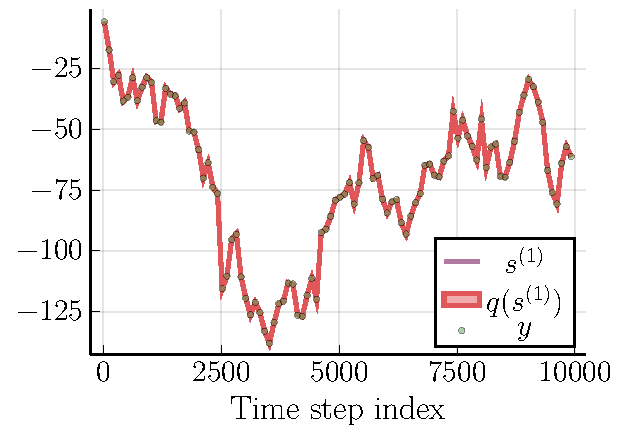
\includegraphics{contents/05-experiments/plots/hgf/04-hierarchical_example_inference_states_2.pdf}
    }
    \caption{Simulated evolution of the layer $s_t^{(1)}$ and its corresponding inferred posterior distribution.}
    \label{fig:sim:hgf_inference_state_1}
  \end{subfigure}
  \hfill
  \begin{subfigure}[t]{0.315\textwidth}
    \centering
    \resizebox{\textwidth}{!}{
        % % Recommended preamble:
% \usetikzlibrary{arrows.meta}
% \usetikzlibrary{backgrounds}
% \usepgfplotslibrary{patchplots}
% \usepgfplotslibrary{fillbetween}
% \pgfplotsset{%
%     layers/standard/.define layer set={%
%         background,axis background,axis grid,axis ticks,axis lines,axis tick labels,pre main,main,axis descriptions,axis foreground%
%     }{
%         grid style={/pgfplots/on layer=axis grid},%
%         tick style={/pgfplots/on layer=axis ticks},%
%         axis line style={/pgfplots/on layer=axis lines},%
%         label style={/pgfplots/on layer=axis descriptions},%
%         legend style={/pgfplots/on layer=axis descriptions},%
%         title style={/pgfplots/on layer=axis descriptions},%
%         colorbar style={/pgfplots/on layer=axis descriptions},%
%         ticklabel style={/pgfplots/on layer=axis tick labels},%
%         axis background@ style={/pgfplots/on layer=axis background},%
%         3d box foreground style={/pgfplots/on layer=axis foreground},%
%     },
% }

\begin{tikzpicture}[/tikz/background rectangle/.style={fill={rgb,1:red,1.0;green,1.0;blue,1.0}, fill opacity={1.0}, draw opacity={1.0}}, show background rectangle]
\begin{axis}[point meta max={nan}, point meta min={nan}, legend cell align={left}, legend columns={1}, title={}, title style={at={{(0.5,1)}}, anchor={south}, font={{\fontsize{18 pt}{23.400000000000002 pt}\selectfont}}, color={rgb,1:red,0.0;green,0.0;blue,0.0}, draw opacity={1.0}, rotate={0.0}, align={center}}, legend style={color={rgb,1:red,0.0;green,0.0;blue,0.0}, draw opacity={1.0}, line width={1}, solid, fill={rgb,1:red,1.0;green,1.0;blue,1.0}, fill opacity={1.0}, text opacity={1.0}, font={{\fontsize{14 pt}{18.2 pt}\selectfont}}, text={rgb,1:red,0.0;green,0.0;blue,0.0}, cells={anchor={center}}, at={(0.98, 0.98)}, anchor={north east}}, axis background/.style={fill={rgb,1:red,1.0;green,1.0;blue,1.0}, opacity={1.0}}, anchor={north west}, xshift={1.0mm}, yshift={-1.0mm}, width={99.6mm}, height={74.2mm}, scaled x ticks={false}, xlabel={Variational iteration index}, x tick style={color={rgb,1:red,0.0;green,0.0;blue,0.0}, opacity={1.0}}, x tick label style={color={rgb,1:red,0.0;green,0.0;blue,0.0}, opacity={1.0}, rotate={0}}, xlabel style={at={(ticklabel cs:0.5)}, anchor=near ticklabel, at={{(ticklabel cs:0.5)}}, anchor={near ticklabel}, font={{\fontsize{16 pt}{20.8 pt}\selectfont}}, color={rgb,1:red,0.0;green,0.0;blue,0.0}, draw opacity={1.0}, rotate={0.0}}, xmajorgrids={true}, xmin={0.8799999999999999}, xmax={5.12}, xticklabels={{$1$,$2$,$3$,$4$,$5$}}, xtick={{1.0,2.0,3.0,4.0,5.0}}, xtick align={inside}, xticklabel style={font={{\fontsize{14 pt}{18.2 pt}\selectfont}}, color={rgb,1:red,0.0;green,0.0;blue,0.0}, draw opacity={1.0}, rotate={0.0}}, x grid style={color={rgb,1:red,0.0;green,0.0;blue,0.0}, draw opacity={0.1}, line width={0.5}, solid}, axis x line*={left}, x axis line style={color={rgb,1:red,0.0;green,0.0;blue,0.0}, draw opacity={1.0}, line width={1}, solid}, scaled y ticks={false}, ylabel={Bethe Free Energy}, y tick style={color={rgb,1:red,0.0;green,0.0;blue,0.0}, opacity={1.0}}, y tick label style={color={rgb,1:red,0.0;green,0.0;blue,0.0}, opacity={1.0}, rotate={0}}, ylabel style={at={(ticklabel cs:0.5)}, anchor=near ticklabel, at={{(ticklabel cs:0.5)}}, anchor={near ticklabel}, font={{\fontsize{16 pt}{20.8 pt}\selectfont}}, color={rgb,1:red,0.0;green,0.0;blue,0.0}, draw opacity={1.0}, rotate={0.0}}, ymajorgrids={true}, ymin={1.3537661894130288}, ymax={1.3588737379406222}, yticklabels={{$1.354$,$1.355$,$1.356$,$1.357$,$1.358$}}, ytick={{1.354,1.355,1.356,1.357,1.358}}, ytick align={inside}, yticklabel style={font={{\fontsize{14 pt}{18.2 pt}\selectfont}}, color={rgb,1:red,0.0;green,0.0;blue,0.0}, draw opacity={1.0}, rotate={0.0}}, y grid style={color={rgb,1:red,0.0;green,0.0;blue,0.0}, draw opacity={0.1}, line width={0.5}, solid}, axis y line*={left}, y axis line style={color={rgb,1:red,0.0;green,0.0;blue,0.0}, draw opacity={1.0}, line width={1}, solid}, colorbar={false}]
    \addplot[color={rgb,1:red,0.0;green,0.6056;blue,0.9787}, name path={febf5715-4f1a-486f-9887-7772927a61c8}, draw opacity={1.0}, line width={1}, solid]
        table[row sep={\\}]
        {
            \\
            1.0  1.3587291846804073  \\
            2.0  1.35401669218457  \\
            3.0  1.353921610870807  \\
            4.0  1.3539111089404197  \\
            5.0  1.353910742673244  \\
        }
        ;
    \addlegendentry {Bethe Free Energy}
\end{axis}
\end{tikzpicture}

        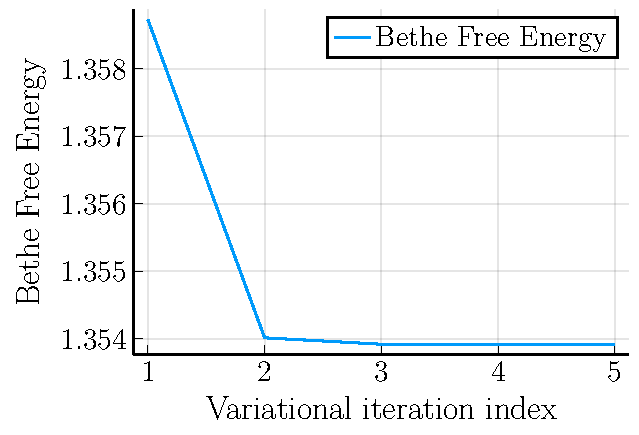
\includegraphics{contents/05-experiments/plots/hgf/04-hierarchical_example_inference_free_energy.pdf}
    }
    \caption{Bethe Free Energy evaluation results.
      The x-axis represents an index of \ac{vmp} iteration.
      The y-axis represents a Bethe Free Energy value at a specific \ac{vmp} iteration.
    }
    \label{fig:sim:hgf_inference_free_energy}
  \end{subfigure}
  \caption{
    Simulated evolution of the 2-layer \ac{hgf} model \eqref{eq:sim:hgf} for $10,000$ synthetically generated 1-dimensional observations with link function $f(s) = exp(\kappa s + \zeta)$, where $\kappa = 1$ and $\zeta = 0$.
    The noise component $\Sigma$ is set to be $10^{-4}$, the noise component $\Omega$ is set to be
    $0.0625$.
    The shaded area shows three standard deviations of the inferred posteriors.
  }
  \label{fig:sim:hgf_inference_states}
\end{figure}

\subsection{Scalability and performance characteristics}

\begin{figure}
  \centering
  \resizebox{\textwidth}{!}{
    % % Recommended preamble:
% \usetikzlibrary{arrows.meta}
% \usetikzlibrary{backgrounds}
% \usepgfplotslibrary{patchplots}
% \usepgfplotslibrary{fillbetween}
% \pgfplotsset{%
%     layers/standard/.define layer set={%
%         background,axis background,axis grid,axis ticks,axis lines,axis tick labels,pre main,main,axis descriptions,axis foreground%
%     }{
%         grid style={/pgfplots/on layer=axis grid},%
%         tick style={/pgfplots/on layer=axis ticks},%
%         axis line style={/pgfplots/on layer=axis lines},%
%         label style={/pgfplots/on layer=axis descriptions},%
%         legend style={/pgfplots/on layer=axis descriptions},%
%         title style={/pgfplots/on layer=axis descriptions},%
%         colorbar style={/pgfplots/on layer=axis descriptions},%
%         ticklabel style={/pgfplots/on layer=axis tick labels},%
%         axis background@ style={/pgfplots/on layer=axis background},%
%         3d box foreground style={/pgfplots/on layer=axis foreground},%
%     },
% }

\begin{tikzpicture}[/tikz/background rectangle/.style={fill={rgb,1:red,1.0;green,1.0;blue,1.0}, fill opacity={1.0}, draw opacity={1.0}}, show background rectangle]
\begin{axis}[point meta max={nan}, point meta min={nan}, legend cell align={left}, legend columns={1}, title={}, title style={at={{(0.5,1)}}, anchor={south}, font={{\fontsize{18 pt}{23.400000000000002 pt}\selectfont}}, color={rgb,1:red,0.0;green,0.0;blue,0.0}, draw opacity={1.0}, rotate={0.0}, align={center}}, legend style={color={rgb,1:red,0.0;green,0.0;blue,0.0}, draw opacity={1.0}, line width={1}, solid, fill={rgb,1:red,1.0;green,1.0;blue,1.0}, fill opacity={1.0}, text opacity={1.0}, font={{\fontsize{14 pt}{18.2 pt}\selectfont}}, text={rgb,1:red,0.0;green,0.0;blue,0.0}, cells={anchor={west}}, at={(0.98, 0.02)}, anchor={south east}}, axis background/.style={fill={rgb,1:red,1.0;green,1.0;blue,1.0}, opacity={1.0}}, anchor={north west}, xshift={1.0mm}, yshift={-1.0mm}, width={226.6mm}, height={86.9mm}, scaled x ticks={false}, xlabel={Number of observation (log-scale)}, x tick style={color={rgb,1:red,0.0;green,0.0;blue,0.0}, opacity={1.0}}, x tick label style={color={rgb,1:red,0.0;green,0.0;blue,0.0}, opacity={1.0}, rotate={0}}, xlabel style={at={(ticklabel cs:0.5)}, anchor=near ticklabel, at={{(ticklabel cs:0.5)}}, anchor={near ticklabel}, font={{\fontsize{16 pt}{20.8 pt}\selectfont}}, color={rgb,1:red,0.0;green,0.0;blue,0.0}, draw opacity={1.0}, rotate={0.0}}, xmode={log}, log basis x={10}, xmajorgrids={true}, xmin={7.585775750291836}, xmax={131825.67385564075}, xticklabels={{$10^1$,$10^2$,$10^3$,$10^4$,$10^5$}}, xtick={{10,100,1000,10000,100000}}, xtick align={inside}, xticklabel style={font={{\fontsize{14 pt}{18.2 pt}\selectfont}}, color={rgb,1:red,0.0;green,0.0;blue,0.0}, draw opacity={1.0}, rotate={0.0}}, x grid style={color={rgb,1:red,0.0;green,0.0;blue,0.0}, draw opacity={0.1}, line width={0.5}, solid}, axis x line*={left}, x axis line style={color={rgb,1:red,0.0;green,0.0;blue,0.0}, draw opacity={1.0}, line width={1}, solid}, scaled y ticks={false}, ylabel={Time (in ms, log-scale)}, y tick style={color={rgb,1:red,0.0;green,0.0;blue,0.0}, opacity={1.0}}, y tick label style={color={rgb,1:red,0.0;green,0.0;blue,0.0}, opacity={1.0}, rotate={0}}, ylabel style={at={(ticklabel cs:0.5)}, anchor=near ticklabel, at={{(ticklabel cs:0.5)}}, anchor={near ticklabel}, font={{\fontsize{16 pt}{20.8 pt}\selectfont}}, color={rgb,1:red,0.0;green,0.0;blue,0.0}, draw opacity={1.0}, rotate={0.0}}, ymode={log}, log basis y={10}, ymajorgrids={true}, ymin={0.1}, ymax={1.0e6}, yticklabels={{$10^{-1}$,$10^{0}$,$10^{1}$,$10^{2}$,$10^{3}$,$10^{4}$,$10^5$,$10^6$}}, ytick={{0.1,1.0,10.0,100.0,1000.0,10000.0,100000.0,1.0e6}}, ytick align={inside}, yticklabel style={font={{\fontsize{14 pt}{18.2 pt}\selectfont}}, color={rgb,1:red,0.0;green,0.0;blue,0.0}, draw opacity={1.0}, rotate={0.0}}, y grid style={color={rgb,1:red,0.0;green,0.0;blue,0.0}, draw opacity={0.1}, line width={0.5}, solid}, axis y line*={left}, y axis line style={color={rgb,1:red,0.0;green,0.0;blue,0.0}, draw opacity={1.0}, line width={1}, solid}, colorbar={false}]
    \addplot[color={rgb,1:red,0.0;green,0.6056;blue,0.9787}, name path={b15436e0-7789-44d4-adba-9fd4d8234e94}, draw opacity={1.0}, line width={1}, solid, mark={triangle*}, mark size={3.0 pt}, mark repeat={1}, mark options={color={rgb,1:red,0.0;green,0.0;blue,0.0}, draw opacity={1.0}, fill={rgb,1:red,0.0;green,0.6056;blue,0.9787}, fill opacity={1.0}, line width={0.75}, rotate={0}, solid}]
        table[row sep={\\}]
        {
            \\
            10.0  0.4315  \\
            20.0  0.7331  \\
            30.0  1.0663  \\
            100.0  3.1955  \\
            300.0  9.3212  \\
            500.0  15.4309  \\
            700.0  21.7392  \\
            1000.0  30.9804  \\
            3000.0  92.092  \\
            5000.0  155.2424  \\
            7000.0  216.4502  \\
            10000.0  306.9206  \\
            30000.0  979.1397  \\
            50000.0  1562.5644  \\
            70000.0  2215.5032  \\
            100000.0  3165.3835  \\
        }
        ;
    \addlegendentry {Reactive MP}
    \addplot[color={rgb,1:red,0.8889;green,0.4356;blue,0.2781}, name path={9f987ce9-b428-449b-ab6f-d128750f590d}, draw opacity={1.0}, line width={1}, dashed, mark={triangle*}, mark size={3.0 pt}, mark repeat={1}, mark options={color={rgb,1:red,0.0;green,0.0;blue,0.0}, draw opacity={1.0}, fill={rgb,1:red,0.8889;green,0.4356;blue,0.2781}, fill opacity={1.0}, line width={0.75}, rotate={180}, solid}]
        table[row sep={\\}]
        {
            \\
            10.0  6.7619  \\
            20.0  13.5798  \\
            30.0  20.4546  \\
            100.0  68.2079  \\
            300.0  206.7111  \\
        }
        ;
    \addlegendentry {Scheduled MP (inference)}
    \addplot[color={rgb,1:red,0.2422;green,0.6433;blue,0.3044}, name path={c238d3f5-cd32-4311-8dcb-ec179cc65982}, draw opacity={1.0}, line width={1}, dashed, mark={triangle*}, mark size={3.0 pt}, mark repeat={1}, mark options={color={rgb,1:red,0.0;green,0.0;blue,0.0}, draw opacity={1.0}, fill={rgb,1:red,0.2422;green,0.6433;blue,0.3044}, fill opacity={1.0}, line width={0.75}, rotate={270}, solid}]
        table[row sep={\\}]
        {
            \\
            10.0  252.56  \\
            20.0  257.965  \\
            30.0  257.8601  \\
            100.0  257.6473  \\
            300.0  255.883  \\
        }
        ;
    \addlegendentry {Scheduled MP (compilation)}
    \addplot[color={rgb,1:red,0.7644;green,0.4441;blue,0.8243}, name path={2150c3b6-9adb-4c15-aadd-118c7691217b}, draw opacity={1.0}, line width={1}, dotted, mark={triangle*}, mark size={3.0 pt}, mark repeat={1}, mark options={color={rgb,1:red,0.0;green,0.0;blue,0.0}, draw opacity={1.0}, fill={rgb,1:red,0.7644;green,0.4441;blue,0.8243}, fill opacity={1.0}, line width={0.75}, rotate={90}, solid}]
        table[row sep={\\}]
        {
            \\
            10.0  3866.7066  \\
            20.0  8099.2013  \\
            30.0  12282.4029  \\
            100.0  41746.4358  \\
            300.0  120336.0759  \\
        }
        ;
    \addlegendentry {NUTS (100)}
    \addplot[color={rgb,1:red,0.6755;green,0.5557;blue,0.0942}, name path={08d41fab-29aa-42f9-a576-5f85198b2541}, draw opacity={1.0}, line width={1}, dotted, mark={diamond*}, mark size={3.0 pt}, mark repeat={1}, mark options={color={rgb,1:red,0.0;green,0.0;blue,0.0}, draw opacity={1.0}, fill={rgb,1:red,0.6755;green,0.5557;blue,0.0942}, fill opacity={1.0}, line width={0.75}, rotate={0}, solid}]
        table[row sep={\\}]
        {
            \\
            10.0  9051.1129  \\
            20.0  18286.9567  \\
            30.0  27829.6717  \\
            100.0  89140.8722  \\
            300.0  264435.7674  \\
        }
        ;
    \addlegendentry {NUTS (200)}
\end{axis}
\end{tikzpicture}

    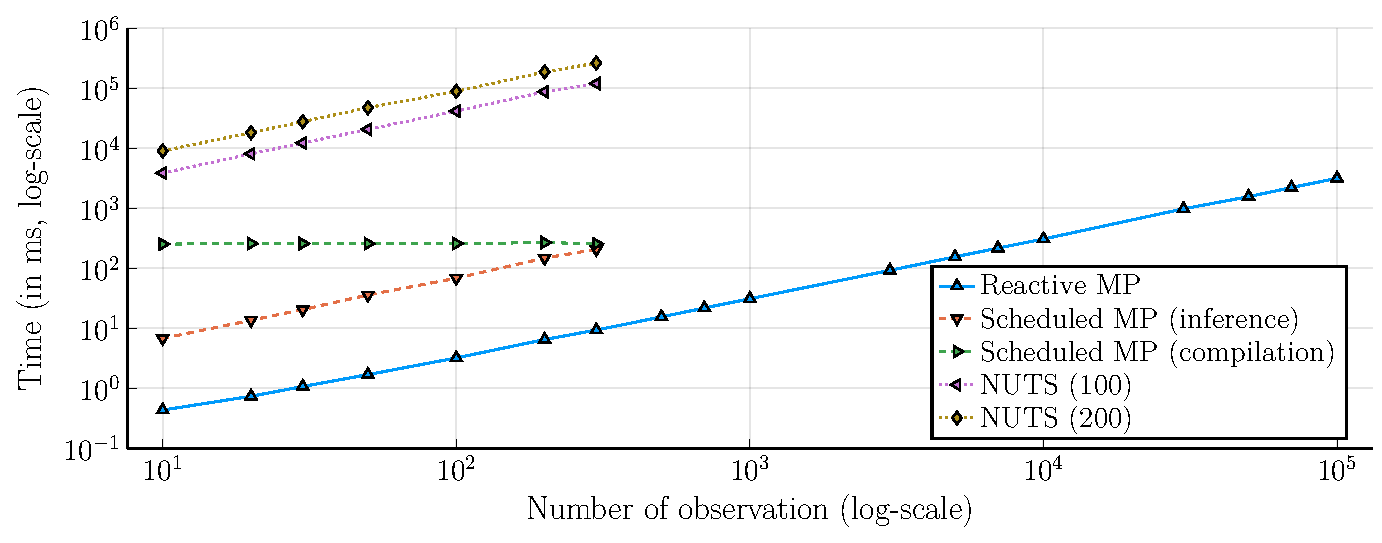
\includegraphics{contents/05-experiments/plots/hgf/04-benchmark_comparison.pdf}
  }
  \caption{A comparison of the runtime duration in milliseconds for automated Bayesian inference in a 2-layer \ac{hgf}~\eqref{eq:sim:hgf} using different methods: reactive message passing (RxInfer), scheduled message passing (ForneyLab), and \ac{nuts} (Turing).
    The values in the figure represent the minimum duration across multiple runs.
    The RxInfer timings include the graph creation time.
    The ForneyLab pipeline involves model compilation, followed by actual inference execution.
    Turing uses \ac{nuts} sampling with 100 and 200 samples, respectively.
    We present benchmark results for more than $300$ observations only for the RxInfer framework.
  }
  \label{fig:sim:hgf_performance_comparison}
\end{figure}

\begin{table}[t]
  \centering
  \begin{tabular}{ |l||r|r|r|r|r|r| }
    \hline
                  & \multicolumn{6}{|c|}{Number of observations}                                                                            \\
    \hline
                  & \multicolumn{3}{|c|}{$s^{(2)}_t$ layer}      & \multicolumn{3}{|c|}{$s^{(1)_t}$ layer}                                  \\
    \hline
                  & 50                                           & 100                                     & 200  & 50    & 100    & 200    \\
    \hline
    VMP (5 iters) & 0.30                                         & 0.18                                    & 0.12 & 0.16  & 0.15   & 0.15   \\
    \hline
    NUTS (100)    & 0.34                                         & 0.27                                    & 0.26 & 65.86 & 140.96 & 364.40 \\
    NUTS (200)    & 0.18                                         & 0.30                                    & 0.14 & 69.01 & 147.88 & 365.02 \\
    \hline
  \end{tabular}
  \caption{Comparison of posterior results accuracy in terms of metric \eqref{eq:sim:average_mse} in the \ac{hgf}~\eqref{eq:sim:hgf} across different methods: message passing (RxInfer and ForneyLab) and \ac{nuts} (Turing).
    Lower values indicate better performance.
    RxInfer and ForneyLab perform online learning with \ac{vmp} on a single time step of the
    corresponding graph.
    The number of \ac{vmp} iterations is set to 5.
    Turing.jl runs two benchmarks with 100 and 200 number of samples respectively.
  }
  \label{table:sim:hgf_accuracy_comparison}
\end{table}

\begin{figure}
  \centering
  \begin{subfigure}[t]{\textwidth}
    \centering
    \resizebox{\textwidth}{!}{
        % % Recommended preamble:
% \usetikzlibrary{arrows.meta}
% \usetikzlibrary{backgrounds}
% \usepgfplotslibrary{patchplots}
% \usepgfplotslibrary{fillbetween}
% \pgfplotsset{%
%     layers/standard/.define layer set={%
%         background,axis background,axis grid,axis ticks,axis lines,axis tick labels,pre main,main,axis descriptions,axis foreground%
%     }{
%         grid style={/pgfplots/on layer=axis grid},%
%         tick style={/pgfplots/on layer=axis ticks},%
%         axis line style={/pgfplots/on layer=axis lines},%
%         label style={/pgfplots/on layer=axis descriptions},%
%         legend style={/pgfplots/on layer=axis descriptions},%
%         title style={/pgfplots/on layer=axis descriptions},%
%         colorbar style={/pgfplots/on layer=axis descriptions},%
%         ticklabel style={/pgfplots/on layer=axis tick labels},%
%         axis background@ style={/pgfplots/on layer=axis background},%
%         3d box foreground style={/pgfplots/on layer=axis foreground},%
%     },
% }

\begin{tikzpicture}[/tikz/background rectangle/.style={fill={rgb,1:red,1.0;green,1.0;blue,1.0}, fill opacity={1.0}, draw opacity={1.0}}, show background rectangle]
\begin{axis}[point meta max={nan}, point meta min={nan}, legend cell align={left}, legend columns={2}, title={}, title style={at={{(0.5,1)}}, anchor={south}, font={{\fontsize{18 pt}{23.400000000000002 pt}\selectfont}}, color={rgb,1:red,0.0;green,0.0;blue,0.0}, draw opacity={1.0}, rotate={0.0}, align={center}}, legend style={color={rgb,1:red,0.0;green,0.0;blue,0.0}, draw opacity={1.0}, line width={1}, solid, fill={rgb,1:red,1.0;green,1.0;blue,1.0}, fill opacity={1.0}, text opacity={1.0}, font={{\fontsize{14 pt}{18.2 pt}\selectfont}}, text={rgb,1:red,0.0;green,0.0;blue,0.0}, cells={anchor={west}}, at={(0.5, 1.02)}, anchor={south}}, axis background/.style={fill={rgb,1:red,1.0;green,1.0;blue,1.0}, opacity={1.0}}, anchor={north west}, xshift={1.0mm}, yshift={-1.0mm}, width={201.2mm}, height={74.2mm}, scaled x ticks={false}, xlabel={Number of observations in dataset (log10-scale)}, x tick style={color={rgb,1:red,0.0;green,0.0;blue,0.0}, opacity={1.0}}, x tick label style={color={rgb,1:red,0.0;green,0.0;blue,0.0}, opacity={1.0}, rotate={0}}, xlabel style={at={(ticklabel cs:0.5)}, anchor=near ticklabel, at={{(ticklabel cs:0.5)}}, anchor={near ticklabel}, font={{\fontsize{16 pt}{20.8 pt}\selectfont}}, color={rgb,1:red,0.0;green,0.0;blue,0.0}, draw opacity={1.0}, rotate={0.0}}, xmode={log}, log basis x={10}, xmajorgrids={true}, xmin={7.585775750291836}, xmax={131825.67385564075}, xticklabels={{$10^1$,$10^2$,$10^3$,$10^4$,$10^5$}}, xtick={{10,100,1000,10000,100000}}, xtick align={inside}, xticklabel style={font={{\fontsize{14 pt}{18.2 pt}\selectfont}}, color={rgb,1:red,0.0;green,0.0;blue,0.0}, draw opacity={1.0}, rotate={0.0}}, x grid style={color={rgb,1:red,0.0;green,0.0;blue,0.0}, draw opacity={0.1}, line width={0.5}, solid}, axis x line*={left}, x axis line style={color={rgb,1:red,0.0;green,0.0;blue,0.0}, draw opacity={1.0}, line width={1}, solid}, scaled y ticks={false}, ylabel={Time (in ms, log10-scale)}, y tick style={color={rgb,1:red,0.0;green,0.0;blue,0.0}, opacity={1.0}}, y tick label style={color={rgb,1:red,0.0;green,0.0;blue,0.0}, opacity={1.0}, rotate={0}}, ylabel style={at={(ticklabel cs:0.5)}, anchor=near ticklabel, at={{(ticklabel cs:0.5)}}, anchor={near ticklabel}, font={{\fontsize{16 pt}{20.8 pt}\selectfont}}, color={rgb,1:red,0.0;green,0.0;blue,0.0}, draw opacity={1.0}, rotate={0.0}}, ymode={log}, log basis y={10}, ymajorgrids={true}, ymin={0.1}, ymax={100000.0}, yticklabels={{$10^{-1}$,$10^{0}$,$10^{1}$,$10^{2}$,$10^{3}$,$10^{4}$,$10^{5}$}}, ytick={{0.1,1.0,10.0,100.0,1000.0,10000.0,100000.0}}, ytick align={inside}, yticklabel style={font={{\fontsize{14 pt}{18.2 pt}\selectfont}}, color={rgb,1:red,0.0;green,0.0;blue,0.0}, draw opacity={1.0}, rotate={0.0}}, y grid style={color={rgb,1:red,0.0;green,0.0;blue,0.0}, draw opacity={0.1}, line width={0.5}, solid}, axis y line*={left}, y axis line style={color={rgb,1:red,0.0;green,0.0;blue,0.0}, draw opacity={1.0}, line width={1}, solid}, colorbar={false}]
    \addplot[color={rgb,1:red,0.3059;green,0.4745;blue,0.6549}, name path={d581c56f-aaf1-4633-a50f-ab6d23cf33f9}, draw opacity={1.0}, line width={1}, solid, mark={diamond*}, mark size={3.0 pt}, mark repeat={1}, mark options={color={rgb,1:red,0.0;green,0.0;blue,0.0}, draw opacity={1.0}, fill={rgb,1:red,0.3059;green,0.4745;blue,0.6549}, fill opacity={1.0}, line width={0.75}, rotate={0}, solid}]
        table[row sep={\\}]
        {
            \\
            10.0  0.4315  \\
            20.0  0.7331  \\
            30.0  1.0663  \\
            50.0  1.6845  \\
            100.0  3.1955  \\
            200.0  6.4795  \\
            300.0  9.3212  \\
            500.0  15.4309  \\
            700.0  21.7392  \\
            1000.0  30.9804  \\
            3000.0  92.092  \\
            5000.0  155.2424  \\
            7000.0  216.4502  \\
            10000.0  306.9206  \\
            30000.0  979.1397  \\
            50000.0  1562.5644  \\
            70000.0  2215.5032  \\
            100000.0  3165.3835  \\
        }
        ;
    \addlegendentry {3 iterations}
    \addplot[color={rgb,1:red,0.949;green,0.5569;blue,0.1686}, name path={74fe8840-82b9-4868-ad3a-b3cccd6e7e94}, draw opacity={1.0}, line width={1}, dashed, mark={*}, mark size={3.0 pt}, mark repeat={1}, mark options={color={rgb,1:red,0.0;green,0.0;blue,0.0}, draw opacity={1.0}, fill={rgb,1:red,0.949;green,0.5569;blue,0.1686}, fill opacity={1.0}, line width={0.75}, rotate={0}, solid}]
        table[row sep={\\}]
        {
            \\
            10.0  0.6456  \\
            20.0  1.1567  \\
            30.0  1.6744  \\
            50.0  2.7448  \\
            100.0  5.1953  \\
            200.0  10.6134  \\
            300.0  15.4119  \\
            500.0  25.5958  \\
            700.0  35.7002  \\
            1000.0  51.1289  \\
            3000.0  152.9888  \\
            5000.0  255.4111  \\
            7000.0  366.5118  \\
            10000.0  512.6566  \\
            30000.0  1546.797  \\
            50000.0  2662.1589  \\
            70000.0  3661.5947  \\
            100000.0  5162.338  \\
        }
        ;
    \addlegendentry {5 iterations}
    \addplot[color={rgb,1:red,0.8824;green,0.3412;blue,0.349}, name path={66f78ad3-ebb7-4c6d-b85f-b06816b2d7dd}, draw opacity={1.0}, line width={1}, dotted, mark={square*}, mark size={3.0 pt}, mark repeat={1}, mark options={color={rgb,1:red,0.0;green,0.0;blue,0.0}, draw opacity={1.0}, fill={rgb,1:red,0.8824;green,0.3412;blue,0.349}, fill opacity={1.0}, line width={0.75}, rotate={0}, solid}]
        table[row sep={\\}]
        {
            \\
            10.0  1.1486  \\
            20.0  2.1796  \\
            30.0  3.1385  \\
            50.0  5.3404  \\
            100.0  10.2956  \\
            200.0  20.9034  \\
            300.0  30.7604  \\
            500.0  51.0307  \\
            700.0  71.0889  \\
            1000.0  101.6726  \\
            3000.0  306.3463  \\
            5000.0  507.9857  \\
            7000.0  730.3044  \\
            10000.0  1023.7101  \\
            30000.0  3135.6569  \\
            50000.0  5125.1793  \\
            70000.0  7378.6533  \\
            100000.0  10502.3322  \\
        }
        ;
    \addlegendentry {10 iterations}
    \addplot[color={rgb,1:red,0.4627;green,0.7176;blue,0.698}, name path={089c873d-8bf7-40d5-854e-0b2b96b48420}, draw opacity={1.0}, line width={1}, dashdotted, mark={triangle*}, mark size={3.0 pt}, mark repeat={1}, mark options={color={rgb,1:red,0.0;green,0.0;blue,0.0}, draw opacity={1.0}, fill={rgb,1:red,0.4627;green,0.7176;blue,0.698}, fill opacity={1.0}, line width={0.75}, rotate={0}, solid}]
        table[row sep={\\}]
        {
            \\
            10.0  2.1807  \\
            20.0  4.183  \\
            30.0  6.1758  \\
            50.0  10.5072  \\
            100.0  20.5674  \\
            200.0  42.5915  \\
            300.0  60.7581  \\
            500.0  101.6792  \\
            700.0  141.984  \\
            1000.0  205.3108  \\
            3000.0  611.7559  \\
            5000.0  1021.3451  \\
            7000.0  1428.5972  \\
            10000.0  2078.2337  \\
            30000.0  6293.4465  \\
            50000.0  10292.5744  \\
            70000.0  14479.5076  \\
            100000.0  20609.9497  \\
        }
        ;
    \addlegendentry {20 iterations}
\end{axis}
\end{tikzpicture}

        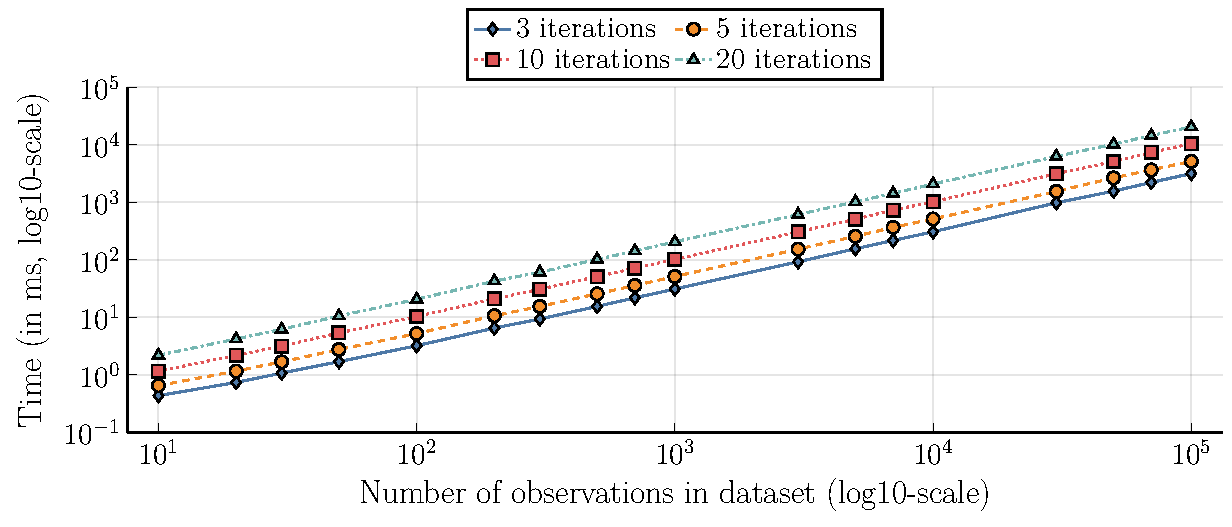
\includegraphics{contents/05-experiments/plots/hgf/04-rxinfer_hgf_scalability_size.pdf}
    }
    \caption{
      Scalability benchmark for different number of performed \ac{vmp} iterations with respect to number of observations in dataset.
    }
    \label{fig:sim:hgf_scalability_size}
  \end{subfigure}
  \hfill
  \begin{subfigure}[t]{\textwidth}
    \centering
    \resizebox{\textwidth}{!}{
        % % Recommended preamble:
% \usetikzlibrary{arrows.meta}
% \usetikzlibrary{backgrounds}
% \usepgfplotslibrary{patchplots}
% \usepgfplotslibrary{fillbetween}
% \pgfplotsset{%
%     layers/standard/.define layer set={%
%         background,axis background,axis grid,axis ticks,axis lines,axis tick labels,pre main,main,axis descriptions,axis foreground%
%     }{
%         grid style={/pgfplots/on layer=axis grid},%
%         tick style={/pgfplots/on layer=axis ticks},%
%         axis line style={/pgfplots/on layer=axis lines},%
%         label style={/pgfplots/on layer=axis descriptions},%
%         legend style={/pgfplots/on layer=axis descriptions},%
%         title style={/pgfplots/on layer=axis descriptions},%
%         colorbar style={/pgfplots/on layer=axis descriptions},%
%         ticklabel style={/pgfplots/on layer=axis tick labels},%
%         axis background@ style={/pgfplots/on layer=axis background},%
%         3d box foreground style={/pgfplots/on layer=axis foreground},%
%     },
% }

\begin{tikzpicture}[/tikz/background rectangle/.style={fill={rgb,1:red,1.0;green,1.0;blue,1.0}, fill opacity={1.0}, draw opacity={1.0}}, show background rectangle]
\begin{axis}[point meta max={nan}, point meta min={nan}, legend cell align={left}, legend columns={2}, title={}, title style={at={{(0.5,1)}}, anchor={south}, font={{\fontsize{18 pt}{23.400000000000002 pt}\selectfont}}, color={rgb,1:red,0.0;green,0.0;blue,0.0}, draw opacity={1.0}, rotate={0.0}, align={center}}, legend style={color={rgb,1:red,0.0;green,0.0;blue,0.0}, draw opacity={1.0}, line width={1}, solid, fill={rgb,1:red,1.0;green,1.0;blue,1.0}, fill opacity={1.0}, text opacity={1.0}, font={{\fontsize{14 pt}{18.2 pt}\selectfont}}, text={rgb,1:red,0.0;green,0.0;blue,0.0}, cells={anchor={west}}, at={(0.5, 1.02)}, anchor={south}}, axis background/.style={fill={rgb,1:red,1.0;green,1.0;blue,1.0}, opacity={1.0}}, anchor={north west}, xshift={1.0mm}, yshift={-1.0mm}, width={201.2mm}, height={74.2mm}, scaled x ticks={false}, xlabel={Number of iterations}, x tick style={color={rgb,1:red,0.0;green,0.0;blue,0.0}, opacity={1.0}}, x tick label style={color={rgb,1:red,0.0;green,0.0;blue,0.0}, opacity={1.0}, rotate={0}}, xlabel style={at={(ticklabel cs:0.5)}, anchor=near ticklabel, at={{(ticklabel cs:0.5)}}, anchor={near ticklabel}, font={{\fontsize{16 pt}{20.8 pt}\selectfont}}, color={rgb,1:red,0.0;green,0.0;blue,0.0}, draw opacity={1.0}, rotate={0.0}}, xmajorgrids={true}, xmin={2.49}, xmax={20.509999999999998}, xticklabels={{3,5,10,20}}, xtick={{3,5,10,20}}, xtick align={inside}, xticklabel style={font={{\fontsize{14 pt}{18.2 pt}\selectfont}}, color={rgb,1:red,0.0;green,0.0;blue,0.0}, draw opacity={1.0}, rotate={0.0}}, x grid style={color={rgb,1:red,0.0;green,0.0;blue,0.0}, draw opacity={0.1}, line width={0.5}, solid}, axis x line*={left}, x axis line style={color={rgb,1:red,0.0;green,0.0;blue,0.0}, draw opacity={1.0}, line width={1}, solid}, scaled y ticks={false}, ylabel={Time (in ms, log10-scale)}, y tick style={color={rgb,1:red,0.0;green,0.0;blue,0.0}, opacity={1.0}}, y tick label style={color={rgb,1:red,0.0;green,0.0;blue,0.0}, opacity={1.0}, rotate={0}}, ylabel style={at={(ticklabel cs:0.5)}, anchor=near ticklabel, at={{(ticklabel cs:0.5)}}, anchor={near ticklabel}, font={{\fontsize{16 pt}{20.8 pt}\selectfont}}, color={rgb,1:red,0.0;green,0.0;blue,0.0}, draw opacity={1.0}, rotate={0.0}}, ymode={log}, log basis y={10}, ymajorgrids={true}, ymin={0.1}, ymax={100000.0}, yticklabels={{$10^{-1}$,$10^{0}$,$10^{1}$,$10^{2}$,$10^{3}$,$10^{4}$,$10^{5}$}}, ytick={{0.1,1.0,10.0,100.0,1000.0,10000.0,100000.0}}, ytick align={inside}, yticklabel style={font={{\fontsize{14 pt}{18.2 pt}\selectfont}}, color={rgb,1:red,0.0;green,0.0;blue,0.0}, draw opacity={1.0}, rotate={0.0}}, y grid style={color={rgb,1:red,0.0;green,0.0;blue,0.0}, draw opacity={0.1}, line width={0.5}, solid}, axis y line*={left}, y axis line style={color={rgb,1:red,0.0;green,0.0;blue,0.0}, draw opacity={1.0}, line width={1}, solid}, colorbar={false}]
    \addplot[color={rgb,1:red,0.3059;green,0.4745;blue,0.6549}, name path={7686c7b2-1869-4449-bf45-8f7efc6fec72}, draw opacity={1.0}, line width={1}, solid, mark={triangle*}, mark size={3.0 pt}, mark repeat={1}, mark options={color={rgb,1:red,0.0;green,0.0;blue,0.0}, draw opacity={1.0}, fill={rgb,1:red,0.3059;green,0.4745;blue,0.6549}, fill opacity={1.0}, line width={0.75}, rotate={0}, solid}]
        table[row sep={\\}]
        {
            \\
            3.0  0.4315  \\
            5.0  0.6456  \\
            10.0  1.1486  \\
            20.0  2.1807  \\
        }
        ;
    \addlegendentry {10 observations}
    \addplot[color={rgb,1:red,0.949;green,0.5569;blue,0.1686}, name path={509ac5b6-83f7-4989-ac40-3ef533f522a7}, draw opacity={1.0}, line width={1}, dashed, mark={triangle*}, mark size={3.0 pt}, mark repeat={1}, mark options={color={rgb,1:red,0.0;green,0.0;blue,0.0}, draw opacity={1.0}, fill={rgb,1:red,0.949;green,0.5569;blue,0.1686}, fill opacity={1.0}, line width={0.75}, rotate={180}, solid}]
        table[row sep={\\}]
        {
            \\
            3.0  30.9804  \\
            5.0  51.1289  \\
            10.0  101.6726  \\
            20.0  205.3108  \\
        }
        ;
    \addlegendentry {1000 observations}
    \addplot[color={rgb,1:red,0.8824;green,0.3412;blue,0.349}, name path={ed9cc609-e972-43ff-9fed-517cace576f3}, draw opacity={1.0}, line width={1}, dotted, mark={triangle*}, mark size={3.0 pt}, mark repeat={1}, mark options={color={rgb,1:red,0.0;green,0.0;blue,0.0}, draw opacity={1.0}, fill={rgb,1:red,0.8824;green,0.3412;blue,0.349}, fill opacity={1.0}, line width={0.75}, rotate={270}, solid}]
        table[row sep={\\}]
        {
            \\
            3.0  306.9206  \\
            5.0  512.6566  \\
            10.0  1023.7101  \\
            20.0  2078.2337  \\
        }
        ;
    \addlegendentry {10000 observations}
    \addplot[color={rgb,1:red,0.4627;green,0.7176;blue,0.698}, name path={c56a334d-6c42-40f8-9491-b35a506ac7f6}, draw opacity={1.0}, line width={1}, dashdotted, mark={triangle*}, mark size={3.0 pt}, mark repeat={1}, mark options={color={rgb,1:red,0.0;green,0.0;blue,0.0}, draw opacity={1.0}, fill={rgb,1:red,0.4627;green,0.7176;blue,0.698}, fill opacity={1.0}, line width={0.75}, rotate={90}, solid}]
        table[row sep={\\}]
        {
            \\
            3.0  3165.3835  \\
            5.0  5162.338  \\
            10.0  10502.3322  \\
            20.0  20609.9497  \\
        }
        ;
    \addlegendentry {100000 observations}
\end{axis}
\end{tikzpicture}

        \includegraphics{contents/05-experiments/plots/hgf/04-rxinfer_hgf_scalability_nits.pdf}
    }
    \caption{Scalability benchmark for different number of observations with respect to number of performed \ac{vmp} iterations.
    }
    \label{fig:sim:hgf_scalability_nits}
  \end{subfigure}
  \caption{    The benchmark for online Bayesian inference for a 2-layer \ac{hgf} system~\eqref{eq:sim:hgf} for RxInfer framework.
    The results demonstrate great scalability of RxInfer framework for different number of
    observations in dataset and for different number of performed \ac{vmp} iterations.
    The values in the table show the minimum possible duration across multiple runs.
    The timings include graph creation time.
  }
  \label{fig:sim:hgf_scalability}
\end{figure}

The main benchmark results are presented in Figure~\ref{fig:sim:hgf_performance_comparison},
and the comparison of the inference accuracy is shown in Table~\ref{table:sim:hgf_accuracy_comparison}.
We demonstrate the performance of the RxInfer framework based on the number of observations
and the number of \ac{vmp} iterations for this particular model in
Figure~\ref{fig:sim:hgf_scalability}.
As in the previous example, we observe that the RxInfer framework scales linearly with both
the number of observations and the number of \ac{vmp} iterations performed (\hyperlink{experiments:scalability}{\emph{Scalability}}).

In this specific example, the inference task in RxInfer for the $10^5$ measurements takes
approximately $3$ seconds, which accounts for $30$ microseconds per measurement.
This efficiency allows the deployment of such models in volatile environments, enabling
real-time continual inference (\hyperlink{experiments:efficiency}{\emph{Run-time efficiency and speed}}).

Unlike the previous examples, where we performed inference on a full graph, the ForneyLab
compilation time no longer depends on the number of observations.
The compilation of the fixed global schedule becomes more acceptable because we always build a single time step of a graph and reuse it during online learning.
Both RxInfer and ForneyLab show the same scalability and posterior accuracy results since they
use the same method for posterior approximation.
However, RxInfer is faster in \ac{vmp} inference execution in absolute timing due to the
architecture proposed in Section~\ref{chapter-03:section:reactive-continual-inference}.
In this architecture, computer resources are used more efficiently as there is no need to
recreate the graph for each new observation of a one-time segment.

In this model, \ac{nuts} algorithm, while being slower in absolute execution time, shows
significantly less accurate results in terms of the metric \eqref{eq:sim:average_mse}, and the
estimated posterior distributions for the first layer start to diverge from their real values  (\hyperlink{experiments:accuracy}{\emph{Posterior accuracy}}).
This outcome may occur because we are restricted to using only one measurement at a time and
performing online (filtering) learning, for which the \ac{nuts} algorithm has not been specifically
designed.
\ac{nuts} typically operates on batches of data, making it difficult to handle streaming data in
real-time scenarios where new observations come one at a time.
Due to these limitations, \ac{nuts} is generally not recommended for real-time dynamical nonstationary
systems, especially when dealing with streaming data or when fast and frequent updates to the
posterior distribution are required.


\section{Related research and experimental evaluations}\label{chapter-05:section:others}

% \subsection*{Experimental evaluations on real-world problems}

The RxInfer framework has undergone extensive testing with sophisticated large-scale
probabilistic models on real-world datasets and problems.
Below, we provide a list of selected\footnote{The full list of research efforts, which use the RxInfer framework can be found on BIASlab website \url{https://biaslab.github.io/publication/}.} PhD dissertations, published papers, and peer-reviewed
articles that have utilized RxInfer for Bayesian inference, along with their abstracts.

\subsubsection*{Message Passing Algorithms for Hierarchical Dynamical Models\\{\small \normalfont \textit{Ismail Senoz}, Eindhoven University of Technology, 2022, PhD dissertation, 171 p, ISBN: 978-90-386-5532-1, \citep{senoz_thesis}}}

This dissertation describes a theoretical framework for deriving customized message
passing-based inference algorithms in factor graphs and illustrates the framework’s
application to hierarchical dynamical models.
Factor graphs are visual representations of the dependency structures among the variables of a
model.
Inference tasks on a given model can be realized using message passing algorithms on the
corresponding factor graph, where propagated messages are computed by integration (summation).
Often, dynamical models of natural processes are constructed hierarchically.
Because the hierarchies in the models may grow the complexity of dependence structures, exact
inference by message passing in these models becomes infeasible and computationally impossible
in a real-time setting.
To employ hierarchical dynamical models in applications that require real-time processing,
inference by message passing needs to be approximated.

\subsubsection*{Message Passing-based Inference in Hierarchical Autoregressive Models\\{\small \normalfont \textit{Albert Podusenko}, Eindhoven: Eindhoven University of Technology, 2022, PhD dissertation. 167 p, ISBN: 978-90-386-5594-9, \citep{podusenko_thesis}}}

This dissertation describes a research effort toward automating personalized design of hearing
aid algorithms through in-the-field communication between a user and a portable intelligent
agent.
The contributions of this thesis are the following.
First, we explore different hierarchical autoregressive models such as continuous
time-varying, switching, and coupled autoregressive models.
We cast these models into a factor graph framework that provides a convenient visualization of
the models.
We show that hierarchical models build on a network of special building blocks that can be
re-used to increase the expressiveness of other dynamical models.
Second, we realize Bayesian inference by an efficient message passing-based algorithm on these
probabilistic factor graphs.
We obtain closed-form message passing update rules for hierarchical autoregressive models.
Third, closing in on the final application, we make use of the developed tools for efficient
inference in hierarchical autoregressive models to build a synthetic agent that tunes hearing
aid parameters under situated conditions.
The developed agent solves the classification of acoustic context, infers optimal trial
design, and executes the HA signal processing algorithm all by automated Bayesian inference.

\subsubsection*{Message Passing-based Inference in the Gamma Mixture Model\\{\small \normalfont \textit{Albert Podusenko, Bart van Erp, Dmitry Bagaev, İsmail Şenöz, Bert de Vries}, 2021 IEEE 31st International Workshop on Machine Learning for Signal Processing (MLSP), Gold Coast, Australia, 2021, pp. 1-6, \url{https://doi.org/10.1109/MLSP52302.2021.9596329}, \citep{podusenko_message_2021}}}

The Gamma mixture model is a flexible probability distribution for representing beliefs about
scale variables such as precisions.
Inference in the Gamma mixture model for all latent variables is non-trivial as it leads to
intractable equations.
This paper presents two variants of variational message passing-based inference in a Gamma
mixture model.
We use moment matching and alternatively expectation-maximization to approximate the posterior
distributions.
The proposed method supports automated inference in factor graphs for large probabilistic
models that contain multiple Gamma mixture models as plug-in factors.
The Gamma mixture model has been implemented in a factor graph package and we present
experimental results for both synthetic and real-world data sets.

\subsubsection*{Message Passing-based Inference in Switching Autoregressive Models\\{\small \normalfont \textit{Albert Podusenko; Bart van Erp; Dmitry Bagaev; Ïsmail şenöz; Bert de Vries}, 2022 30th European Signal Processing Conference (EUSIPCO), Belgrade, Serbia, 2022, pp. 1497-1501, \url{https://doi.org/10.23919/EUSIPCO55093.2022.9909828}, \citep{podusenko_message_2021-1}}}

The switching autoregressive model is a flexible model for signals generated by non-stationary
processes.
Unfortunately, evaluation of the exact posterior distributions of the latent variables for a
switching autoregressive model is analytically intractable, and this limits the applicability
of switching autoregressive models in practical signal processing tasks.
In this paper we present a message passing-based approach for computing approximate posterior
distributions in the switching autoregressive model.
Our solution tracks approximate posterior distributions in a modular way and easily extends to
more complicated model variations.
The proposed message passing algorithm is verified and validated on synthetic and acoustic
data sets respectively.

\subsubsection*{AIDA: An Active Inference-Based Design Agent for Audio Processing Algorithms\\{\small \normalfont \textit{Albert Podusenko , Bart van Erp , Magnus Tønder Koudahl , Bert de Vries}, Frontiers Signal Processing, Sec. Signal Processing Theory, Volume 2, 07 March 2022, \url{https://doi.org/10.3389/frsip.2022.842477}, \citep{podusenko_aida_2022}}}

In this paper we present Active Inference-Based Design Agent (AIDA), which is an active
inference-based agent that iteratively designs a personalized audio processing algorithm
through situated interactions with a human client.
The target application of AIDA is to propose on-the-spot the most interesting alternative
values for the tuning parameters of a hearing aid (HA) algorithm, whenever a HA client is not
satisfied with their HA performance.
AIDA interprets searching for the “most interesting alternative” as an issue of optimal
(acoustic) context-aware Bayesian trial design.
In computational terms, AIDA is realized as an active inference-based agent with an Expected
Free Energy criterion for trial design.
This type of architecture is inspired by neuro-economic models on efficient (Bayesian) trial
design in brains and implies that AIDA comprises generative probabilistic models for acoustic
signals and user responses.
We propose a novel generative model for acoustic signals as a sum of time-varying
auto-regressive filters and a user response model based on a Gaussian Process Classifier.
The full AIDA agent has been implemented in a factor graph for the generative model and all
tasks (parameter learning, acoustic context classification, trial design, etc.) are realized
by variational message passing on the factor graph.
All verification and validation experiments and demonstrations are freely accessible at our
GitHub.

\subsubsection*{Message Passing-based System Identification for NARMAX Models\\{\small \normalfont \textit{Albert Podusenko , Semih Akbayrak , Ismail Senoz , Maarten Schoukens , Wouter Kouw}, 2022 IEEE 61st Conference on Decision and Control (CDC), Cancun, Mexico, 2022, pp. 7309-7314, \url{https://doi.org/10.1109/CDC51059.2022.9992891}, \citep{semih_akbayrak_podusenkoakbayrak-2022-cdc_nodate}}}

The article presents a variational Bayesian identification procedure for polynomial NARMAX
models based on message passing on a factor graph.
Message passing allows us to obtain full posterior distributions for regression coefficients,
precision parameters and noise instances by means of local computations distributed according
to the factorization of the dynamic model.
The posterior distributions are important to shaping the predictive distribution for outputs,
and ultimately lead to superior model performance during 1-step ahead prediction and
simulation.

\subsubsection*{Efficient Model Evidence Computation in Tree-structured Factor Graphs\\{\small \normalfont \textit{Hoang Minh Huu Nguyen , Bart van Erp , Ismail Senoz , Bert de Vries}, 2022 IEEE Workshop on Signal Processing Systems (SiPS), Rennes, France, 2022, pp. 1-6, \url{https://doi.org/10.1109/SiPS55645.2022.9919250}, \citep{nguyen_efficient_2022}}}

Model evidence is a fundamental performance measure in Bayesian machine learning as it
represents how well a model fits an observed data set.
Since model evidence is often an intractable quantity, the literature often resorts to
computing instead the Bethe Free Energy (BFE), which for cycle-free models is a tractable
upper bound on the (negative log-) model evidence.
In this paper, we propose a different and faster evidence computation approach by tracking
local normalization constants of sum-product messages, termed scale factors.
We tabulate scale factor update rules for various elementary factor nodes and by experimental
validation we verify the correctness of these update rules for models involving both discrete
and continuous variables.
We show how tracking scale factors leads to performance improvements compared to the
traditional BFE computation approach.

\subsubsection*{Online Single-Microphone Source Separation using Non-Linear Autoregressive Models\\{\small \normalfont \textit{Bart van Erp , Bert de Vries}, Proceedings of The 11th International Conference on Probabilistic Graphical Models, 2022, \url{https://proceedings.mlr.press/v186/erp22a.html}, \citep{van_erp_online_2022}}}

In this paper a modular approach to single-microphone source separation is proposed.
A probabilistic model for mixtures of observations is constructed, where the independent
underlying source signals are described by non-linear autoregressive models.
Source separation in this model is achieved by performing online probabilistic inference
through an efficient message passing procedure.
For retaining tractability with the non-linear autoregressive models, three different
approximation methods are described.
A set of experiments shows the effectiveness of the proposed source separation approach.
The source separation performance of the different approximation methods is quantified through
a set of verification experiments.
Our approach is validated in a speech denoising task.

\subsubsection*{Hybrid Inference with Invertible Neural Networks in Factor Graphs\\{\small \normalfont \textit{Bart van Erp , Bert de Vries}, 2022 30th European Signal Processing Conference (EUSIPCO), Belgrade, Serbia, 2022, pp. 1397-1401, \url{https://doi.org/10.23919/EUSIPCO55093.2022.9909873}, \citep{van_erp_hybrid_2022}}}

This paper bridges the gap in the literature between neural networks and probabilistic
graphical models.
Invertible neural networks are incorporated in factor graphs and inference in this model is
described by linearization of the network.
Consequently, hybrid probabilistic inference in the model is realized through message passing
with local constraints on the Bethe free energy.
We provide the local Bethe free energy for the invertible neural network node, which allows
for evaluation of the performance of the entire probabilistic model.
Experimental results show effective hybrid inference in a neural network-based probabilistic
model for a binary classification task, paving the way towards a novel class of machine
learning models.

\subsection*{More examples}

The RxInfer framework's repository\footnote{RxInfer framework's examples on GitHub repository:
  \url{https://github.com/biaslab/RxInfer.jl/tree/main/examples}} contains numerous small and
large, simple and sophisticated inference examples.
Notably, none of these examples were planned in advance, highlighting the versatility and
generality of the underlying inference implementation.
The RxInfer framework has been designed with efficiency and scalability in mind, providing a
generic framework to run inference in a wide range of complex probabilistic models.
Below is a selection of some examples, but the full list of examples is available on the
official RxInfer framework's GitHub repository.

\begin{itemize}
  \item \textbf{Bayesian Linear Regression} - This example showcases the inference task in a regression probabilistic model \citep{wang_general_2015}.
  \item \textbf{Ensemble Learning of a Hidden Markov Model} - Demonstrates structured variational Bayesian inference in a Hidden Markov Model (HMM) with unknown transition and observational matrices \citep{rabiner_tutorial_1989, ephraim_bayesian_1992}.
  \item \textbf{Autoregressive Model} - Illustrates the inference task in an autoregressive probabilistic model \citep{podusenko_message_2021-1}.
  \item \textbf{Bayesian ARMA (Autoregressive Moving-Average)} - Presents the inference task in an autoregressive moving-average probabilistic model \citep{thiesson_arma_2012, kouw_variational_2021}.
  \item \textbf{System Identification} - An example of a complex inference task involving the system identification problem of two combined signals \citep{peterka_bayesian_1981}.
  \item \textbf{Mixture Models} - Several examples of univariate, multivariate, conjugate, and non-conjugate inference tasks in mixture models \citep{podusenko_message_2021, hao_speech_2010}.
  \item \textbf{Global Hyperparameter Optimization} - Demonstrates that the entire inference task in RxInfer can be auto-differentiated to obtain gradients with respect to hyperparameters of a probabilistic model.
  \item \textbf{Amortized Bayesian Inference with LSTM} - Uses Bayesian inference to train a Long short-term memory (LSTM) neural network and uses the inference results for prediction in a \ac{nlds} \citep{gemici_generative_2017}.
  \item \textbf{Conjugate-Computational Variational Message Passing} - Provides an extensive tutorial for non-conjugate message-passing-based inference with the RxInfer framework, exploiting the local CVI approximation \citep{akbayrak_probabilistic_2022}.
  \item \textbf{Expectation Propagation in Probit Model} - Illustrates the expectation propagation algorithm in the context of state-estimation in a linear state-space model that combines a Gaussian state-evolution model with a discrete observation model \citep{raymond_expectation_2014}.
  \item \textbf{BIFM Kalman Smoothing} - Demonstrates a more efficient than RTS Kalman smoothing procedure \citep{wadehn_new_2016, loeliger_sparsity_2016}.
  \item \textbf{Active Inference Mountain Car} - An example of the Active Inference task for the mountain car problem \citep{van_de_laar_simulating_2019}.
  \item \textbf{Chance-Constrained Active Inference} - Applies reactive message passing for active inference in the context of chance-constraints \citep{van_de_laar_chance-constrained_2021}.
\end{itemize}

I gratefully acknowledge the great support and assistance from the BIASlab group at Eindhoven University of Technology, who contributed to writing and reviewing a comprehensive set of examples for the RxInfer framework.
Their collaboration has helped demonstrate the framework's effectiveness and applicability
across diverse domains and real-world scenarios.

\section{Conclusions}\label{chapter-05:section:conclusion}

In this chapter, we conducted an experimental evaluation of the \ac{rmp} framework, 
which encompasses both exact and approximate Bayesian inference by
minimizing a \ac{cbfe} functional.
The \ac{rmp} framework supports hybrid algorithms with analytical message update rules, including
\ac{bp}, \ac{ep}, \ac{em}, \ac{vmp}, and provides flexibility in terms of variational constraints.

The implementation of \ac{rmp} in the form of RxInfer, developed in the Julia programming language,
showed to be an efficient and scalable realization of an automated \ac{cbfe} minimization process that can be used
as a fast approximate Bayesian inference process.
RxInfer has successfully handled large-scale models with hundreds of thousands of unknowns,
demonstrating its potential for real-world applications.
The RxInfer framework offers a high level of customization through the creation of custom
nodes, message update rules, and approximation methods.

The experimental results on various standard signal processing models revealed substantial
performance improvements of RxInfer compared to alternative Julia-based frameworks for automated Bayesian inference.
The proposed implementation runs smoothly on regular office computers, avoiding the need for
expensive supercomputers or \ac{gpu} support, making it cost-effective for Bayesian inference on
large datasets with hundreds of thousands of observations.

Sampling-based methods, such as \ac{nuts}, suffer from
scalability challenges, making them unsuitable for real-time Bayesian inference applications.
These methods rely on generating samples from the posterior distribution to approximate the
desired results.
However, as the complexity and size of the probabilistic model increase, the number of
required samples also increases.
Consequently, the computational burden becomes prohibitively high, making sampling-based
methods inefficient for large-scale problems with a substantial number of unknowns.
Moreover, sampling-based algorithms often exhibit slow convergence, especially in high-dimensional
spaces, further exacerbating their scalability issues.
As real-time applications demand quick and efficient inference, the time and resources
required for sampling-based methods make them impractical for such scenarios, prompting the
need for alternative approaches, such as \ac{rmp}, which can handle large models
efficiently and provide results in a timely manner.

The benchmark results indicated that the overhead associated with managing the reactive nature of
the architecture is minimal and that \ac{rmp} consistently outperforms the reference message
passing-based implementation.
The lack of explicit scheduling in the proposed architecture provides practical advantages by
avoiding the need to traverse the entire factor graph, thereby saving computational resources.

We believe that the introduction of a reactive programming approach to message passing-based
inference opens up new avenues for further research, bringing real-time Bayesian inference
closer to real-world applications.
The RxInfer framework's ability to handle large models and simplify the model exploration
process in signal processing applications makes it a promising tool for a wide range of
probabilistic modeling tasks.
The framework lays the foundation for advancing the state-of-the-art in Bayesian inference and
promotes the adoption of \ac{rmp} in various fields, encouraging more researchers and practitioners
to explore the benefits of reactive message passing.
As the field of Bayesian inference continues to evolve, we anticipate that the RxInfer framework
will be further refined and extended, contributing to ongoing progress in simulating large-scale Bayesian inference processes.



\null\thispagestyle{empty}\stopthumb
\includepdf[noautoscale, pages=-]{contents/banners/chapter-06.pdf}
\chapter{Discussion and conclusions}
\label{chapter-06}
\begin{quote}
  \emph{\begin{otherlanguage*}{russian}
\textsf{
``Кто не может осилить малого, тому и великое не под силу.''
}
\end{otherlanguage*}}
\end{quote}
\null\hfill  --~\textit{\begin{otherlanguage*}{russian}\textsf{Ломоносов, Михаил Васильевич}\end{otherlanguage*}}\\
\null\hfill\small{a Russian polymath, scientist, and writer, who founded Moscow State University and made important contributions to literature, education, and science}
\addthumb{thumb_chapter_6}{\huge{6}}{white}{black}

\section{Contributions}\label{chapter-06:section:contributions}

This dissertation proposes a novel architecture for simulating difficult Bayesian inference processes.
The designed architecture integrates reactive programming ideas with previous research efforts
in message passing, aiming to address the central research question:

\begin{rqbox}
  \mainquestion
\end{rqbox}

In particular, the work was driven by five concrete research questions, which we discuss next.

\subsection{Scalability}

\begin{questions}
  \item \scalabilityquestion \label{question:contributions:scalability}
\end{questions}

The first sub-question focuses on the scalability of the inference procedure.
In Chapter~\ref{chapter-02}, we presented the \ac{cbfe} minimization procedure, formulated as a localized message passing process on a \ac{tffg}. The main strengths of the advocated solution are the following:
\begin{itemize}
  \item \textbf{Efficient scalability}. The \ac{cbfe} optimization procedure demonstrates exceptional scalability in handling 
        large models with hundreds of thousands of latent states.
        By leveraging the local properties of factor graphs, the message passing-based \ac{cbfe}
        optimization approach efficiently scales to complex and extensive probabilistic models,
        allowing analysis of massive datasets.
  \item \textbf{Unified framework}.
        The \ac{cbfe} minimization procedure establishes a unified framework for well-known Bayesian inference
        algorithms implemented as message passing. 
        This unified approach enables the seamless integration of different algorithms and provides a
        solid mathematical foundation for deriving novel message passing techniques.
  \item \textbf{Trade-off flexibility}.
        The variational formulation and the constrained search space of the \ac{cbfe} minimization offer a
        convenient advantage of striking a balance between computational load and inference
        accuracy. 
        This flexibility allows users to make informed trade-offs according to their specific
        application requirements, making the architecture suitable to a wide range of practical scenarios.
\end{itemize}

In summary, message passing-based \ac{cbfe} optimization forms a strong foundation for scalable
Bayesian inference and for further research and exploration of possible solutions to the
remaining questions.

\subsection{Real-time processing}

\begin{questions}[resume] \item \reactivityquestion
  \label{question:contributions:reactivity}
\end{questions}

The second sub-question addresses the issue of real-time Bayesian inference.
In Chapter~\ref{chapter-03}, we combine reactive programming concepts with \ac{cbfe} minimization
based on message passing, which we call \acf{rmp}.
The nodes and edges of the factor graphs are formulated as reactive primitives that
automatically respond to changes in their local subgraph.
Here are the main strengths of the proposed solution:
\begin{itemize}
  \item \textbf{Real-time processing}.
        Reactivity allows for seamless integration with streaming data and processing observations as soon as they become available.
  \item \textbf{Continual inference}. The \ac{rmp} architecture performs continual Bayesian
        inference, which can reactively adapt to new observations without interrupting the whole inference process.
  \item \textbf{Dynamic environments}.
        Reactivity and adaptivity are crucial components in modeling dynamic environments. These features make the architecture applicable to various real-world applications that involve continuous volatile data streams.        
\end{itemize}


\subsection{Robustness}

\begin{questions}[resume] \item \robustnessquestion
  \label{question:contributions:robustness}
\end{questions}

The third sub-question focuses on the robustness of the inference procedure.
The proposed architecture, in principle, supports adaptations, as nodes and edges depend
solely on changes in their local subgraphs, rather than the global model structure. 
Here are the main strengths of the advocated solution:
\begin{itemize}
  \item \textbf{No explicit schedule required}. 
        Nodes and edges react automatically to changes in their local subgraphs, removing the burden of manually specifying a global fixed message passing schedule and avoiding associated problems. Since no explicit schedule is required, the inference procedure becomes more robust and tolerant to structural changes in the model and may still react and update itself even if the part of the system changes or collapses.
  \item \textbf{Data source independence}.
        \Ac{rmp} seamlessly processes messages locally from dynamic sources by design without interrupting the
        overall inference process. 
        This feature opens up possibilities for robust inference from sources with different update rates, such as
        hardware sensors, Internet data streams, or other unpredictable inputs.
\end{itemize}

Although this dissertation does not deeply explore all the properties of the robust inference
procedure, it opens up a lot of opportunities for future research in this area.

\subsection{User experience}

\begin{questions}[resume] \item \userexperiencequstion
  \label{question:contributions:user-experience}
\end{questions}

The fourth sub-question addresses the user experience provided by the actual implementation.
In Chapter~\ref{chapter-04}, we present the open source framework, which is called RxInfer and
implemented in Julia, the high-performance programming language.
We note the following main benefits of the proposed solution:
\begin{itemize}
  \item
        \textbf{User-friendly framework}. The developed RxInfer framework aims to offer a
        user-friendly experience for researchers and practitioners in the field of Bayesian inference.
        By providing a high-level, human-readable probabilistic model description, researchers can
        easily translate their ideas into corresponding factor graph representations, reducing the
        barrier to entry for probabilistic modeling.
  \item \textbf{Automated inference}.
        The framework also offers automated inference procedures.
        Researchers can conveniently define their desired constraints in a textual and human-readable
        format, allowing the framework to handle the inference process automatically.
        This feature streamlines the experimentation process and reduces the need for manual
        intervention.
  \item \textbf{Educational value}. RxInfer has been effectively utilized as an educational tool, introducing Bayesian inference methodologies to students at the Eindhoven Technical University\footnote{For instance, in the graduate course "Bayesian Machine Learning and Information Processing" (5SSD0), web \url{https://biaslab.github.io/teaching/bmlip/}. Educational materials are available at \url{https://github.com/bertdv/BMLIP}.}.
  In addition, RxInfer has been used to teach fundamentals of message passing-based 
        inferences on YouTube\footnote{Intro to RxInfer.jl | Automatic Bayesian Inference on Factor Graph with Message Passing \url{https://youtu.be/_vVHWzK9NEI}.}.
        Its user-friendly nature and open-source availability facilitate its adoption in educational
        settings, helping students grasp complex probabilistic concepts while gaining practical
        experience with Bayesian inference methods. 
\end{itemize}

\subsection{Utility}

\begin{questions}[resume] \item \utilityquestion
  \label{question:contributions:utility}
\end{questions}

The final sub-question assesses the utility of the proposed architecture.
Chapter~\ref{chapter-05} experimentally evaluates the RxInfer framework in various
large-scale probabilistic models, demonstrating its ability to perform reactive and continual
inferences both on large static data sets and dynamic infinite data streams.
Here are the main conclusions from the extensive set of experiments and applications in Chapter~\ref{chapter-05}:
\begin{itemize}
  \item \textbf{Empirical evaluation}. Chapter~\ref{chapter-05} presents a detailed empirical 
  evaluation of the RxInfer framework on various large-scale probabilistic models.
        The comprehensive evaluation demonstrates its utility and performance across diverse
        applications, validating its effectiveness in reactive and continual inference on infinite
        data streams.
  \item \textbf{Scientific contributions}.
        The utility of RxInfer is supported by various successful applications in complex
        real-world probabilistic modeling projects as evidenced by several scientific publications in high-ranked
        journals and conferences.
        The versatility and robustness of the framework enable researchers to 
        address challenging research problems and to communicate their findings to the scientific community.
   \item \textbf{Versatile approach}.
        The documentation of RxInfer contains dozens of different examples with different probabilistic models and different inference constraints. None of the examples were planned in advance, which emphasizes the versatility and great potential of \ac{cbfe} minimization procedure implemented as message passing.
  % \item \textbf{Universality and Future Potential}.
  %       Despite the remarkable achievements of the framework, the question of universality remains,
  %       paving the way for future research and improvement.
\end{itemize}

Overall, this dissertation provides a novel architecture for robust, scalable, and robust Bayesian inference 
solution for applications where real-time Bayesian inference is required, such as \ac{aif}.
By combining message passing with reactive programming ideas, we have achieved significant
advancements in addressing research questions and contributing to the field of Bayesian
inference.


\section{Potential limitations}\label{chapter-06:section:discussion}

\subsection{Approximate Bayesian inference}

\Ac{vi} and \ac{cbfe} in particular provide an approximate solution to complex
probabilistic inference problems.
In many situations, obtaining an exact solution is unfeasible, and the goal is
to find a "good enough" approximation that serves the practical needs of the application.
Even if exact inference is theoretically feasible, it is not always practical 
due to potentially enormous computational requirements.
\Ac{vi} methods offer a trade-off between accuracy and computational load, making
them a valuable approach when exact inference is not achievable within strict time and memory
constraints.
However, it is essential to consider the implications of approximation carefully. Variational constraints
may significantly reduce the computational load but, at the same time, may lead to a considerable loss of accuracy, rendering the results unusable for certain applications.
Although the dissertation does not delve into the specifics of this trade-off for individual
applications, we would like to highlight the importance of carefully assessing the level of
approximation required and ensuring that the chosen variational inference method meets the
application's specific needs and accuracy requirements.

\subsection{Data-driven scheduling}

The proposed architecture does not involve the creation of an explicit schedule; instead, it
allows nodes and edges to respond to local changes in their subgraphs. 
However, it is important to note that the actual implementation still follows an order
of commands, which is necessary for any algorithm executed on any computer processor. 
The order, although implicit, is based on the arrival of the data and the sequence of reactions 
by the nodes and edges.
This implicit order is considered an implementation detail and is not explicitly specified in the
architecture.

Explicit scheduling in message passing algorithms has been an area of considerable research
effort.
Although the lack of explicit scheduling brings notable advantages to the proposed architecture, 
it is essential to recognize the strengths of explicit scheduling in certain contexts.
One of the key benefits of explicit scheduling is the ease of debugging and examination of the
algorithm, particularly in cases where unexpected behavior or errors occur.
With an explicit schedule, it becomes more straightforward to trace and understand the fixed sequence of computations, aiding in diagnosing issues. 
Additionally, explicit scheduling aligns more naturally with conventional computers that
operate as sequential state machines, making the implementation process more straightforward and
compatible with standard computational architectures.

\subsection{Reactivity for non-reactive applications}

Reactivity, while offering valuable properties, introduces an additional layer of complexity in the actual implementation.
The dynamic nature of reactivity requires careful handling of data dependencies and update
timings, creating extra barriers for newcomers to the field or researchers aiming to
contribute to the architecture.
As the \ac{rmp} architecture embraces continual online adaptations, it is crucial to ensure the correct sequencing of updates, demanding more in-depth expertise in reactive programming and message passing algorithms.
Handling large systems with thousands of reactive actors is inherently challenging, as it
introduces complexities in reasoning about and debugging the code base. 
Most programming languages do not natively support reactive programming, necessitating the
adoption of external libraries to implement reactive design patterns.
Although such libraries often provide tools for debugging and analyzing the flow of reactive
programs, the maturity of these tools can vary, potentially posing challenges in identifying
and addressing issues within reactive applications.
Although these concerns may improve over time and with ongoing development.
As such, imperative programming design may be favored in certain applications where simplicity, 
ease of implementation, and straightforward debugging are of paramount importance, and the added
complexities of reactivity may be deemed unnecessary. 


\section{Future research directions}\label{chapter-06:section:future-research}

In this section, we identify promising areas where further investigation and development can
lead to significant advancements in both theory and application.
By highlighting these future research directions, we aim to inspire and guide researchers and
practitioners towards new horizons in probabilistic modeling and inference techniques in \ac{aif} agents.

\begin{table}
\centering
\begin{tabular}{|l|| C{25mm} | C{25mm} | C{25mm} |} 
 \hline
 \diagbox{Criteria}{Method} & Sampling & Black-box VI & CBFE with RMP \\ [0.5ex] 
 \hline\hline
 Universal & \cellcolor[HTML]{dfffdf} \tikzcmark & \cellcolor[HTML]{dfffdf} \tikzcmark & \cellcolor[HTML]{ffffe0} ?\\ \hline
 Automated & \cellcolor[HTML]{dfffdf} \tikzcmark & \cellcolor[HTML]{dfffdf} \tikzcmark & \cellcolor[HTML]{dfffdf} \tikzcmark\\ \hline
 Scalable & \cellcolor[HTML]{ffdfdf} \tikzxmark & \cellcolor[HTML]{dfffdf} \tikzcmark & \cellcolor[HTML]{dfffdf} \tikzcmark\\ \hline
 Real-time & \cellcolor[HTML]{ffdfdf} \tikzxmark & \cellcolor[HTML]{ffdfdf} \tikzxmark & \cellcolor[HTML]{dfffdf} \tikzcmark\\ \hline
 Adaptable & \cellcolor[HTML]{ffdfdf} \tikzxmark & \cellcolor[HTML]{ffdfdf} \tikzxmark & \cellcolor[HTML]{dfffdf} \tikzcmark\\ \hline
 Continual & \cellcolor[HTML]{ffdfdf} \tikzxmark & \cellcolor[HTML]{ffdfdf} \tikzxmark  & \cellcolor[HTML]{dfffdf} \tikzcmark\\ \hline
 Low-power & \cellcolor[HTML]{ffdfdf} \tikzxmark & \cellcolor[HTML]{ffdfdf} \tikzxmark  & \cellcolor[HTML]{ffffe0} ?\\
 \hline
\end{tabular}
\caption{A (superficial) comparison of popular methodologies for approximate Bayesian inference as in Table~\ref{table:intro:comparison}.
The proposed architecture, based on \ac{cbfe} and implemented as \ac{rmp}, exhibits essential properties for applications where real-time Bayesian inference is required, such as \ac{aif}. 
}
\label{table:contributions:comparison}
\end{table}

The development of the proposed architecture was highly motivated by developing a supporting toolbox for the \ac{aif} agents, which should learn and act autonomously in a dynamic environment. According to \ac{fep}, \ac{aif} agents must perform approximate Bayesian inference, which, in turn, must be scalable, real-time, adaptable, continual, and low power.
RxInfer makes a step forward towards this goal and implements the framework, which is compatible with this requirements. However, related challenges remain before the actual realization of \ac{aif} agents in the field:
\begin{itemize}
    \item \textbf{Model adaptation}. While there are existing papers and demos that encode simple \ac{aif} agents for specific applications with known environmental dynamics, most interesting real-world applications lack a precise model for environmental dynamics. Consequently, a major future research direction lies in developing a framework for adapting the model structure in real-time under \ac{cbfe} minimization pressure.
    \item \textbf{Massive parallelization and asynchronous inference}. In natural agents, multiple sensory data streams and action channels often process data simultaneously, necessitating parallelization of computations.
    \item \textbf{Lazy inference with different update rates}. In addition to the previous direction, multiple sensory data may arrive with different update rates. Support for signals with different update rates is essential for efficient utilization of available computer resources in autonomous systems.
    \item \textbf{Universal and efficient inference}. The proposed architecture has proven to be useful in a broad class of probabilistic models and real-world problems. The actual implementation is, however, not universal yet, in comparison to black-box inference methods, such as \ac{bbvi}.
\end{itemize}

\subsection{Model adaptation}

Considerable effort has been devoted to learning the structure of models from data, however,
the question of automatic model adaptation driven by \ac{cbfe} minimization remains an open challenge \citep{beckers_principled_2022, friston_bayesian_2018}.
In an ideal scenario, a model should possess the capability to adapt dynamically in response
to new observations, effectively becoming a latent state integrated into the inference
process.
The proposed architecture allows for dynamic changes to nodes during the inference process, but
does not address crucial questions such as \textit{which node to change} and \textit{what node to use as a replacement}.
% The current dissertation leaves this question open avenues for future research.
% Potential problems associated with automatic model adaptation include determining the
% appropriate method to change the model effectively, adaptively predicting which model
% alterations might yield improvements, and devising strategies for selecting specific parts of
% the model to modify.
Additionally, the challenge of ensuring the feasibility of rolling back to a previous model
configuration in the event of undesirable adaptations arises as a crucial aspect to be
investigated.
Addressing these questions is important for achieving robust and efficient
model adaptation and represents an exciting frontier for future research in the field.
\begin{figure}
  \centering
  \resizebox{0.85\textwidth}{!}{\begin{tikzpicture}[node distance=5mm, style]

  \tikzset{var/.style={box, circle, inner sep=0mm, minimum size=3mm}}

  \node[box] (b1) {};
  \node[var] (b2) [right=of b1]{};

  \node[var] (b3) [below=of b1]{};  
  \node[box] (b4) [right=of b3]{};  

  % \node[var] (b11) [below=of b1] {};
  % \node[box] (b14) [right=of b11] {};

  \path[line] (b1) edge[-] (b2);
  \path[line] (b2) edge[-] (b4);
  \path[line] (b1) edge[-] (b3);
  \path[line] (b3) edge[-] (b4);

   \node[box, densely dotted] (replace) [fit=(b4)] {};
   \node[node distance=0mm] (replacelabel) [below=of replace] {\scriptsize \textbf{Sub-model \#1}};

   \node[box, node distance=20mm] (r1) [right=of b4] {};
   \node[var] (r2) [right=of r1] {};
   \node[box] (r3) [right=of r2] {};

   \node[] (i1) [above=of r1] {};
   \node[] (i2) [left=of r1] {};

   \path[line] (r1) edge[-] (r2);
   \path[line] (r2) edge[-] (r3);
   \path[line] (r1) edge[-] (i1);
   \path[line] (r1) edge[-] (i2);

   \path[] ([xshift=-5mm, yshift=5mm]r1.west) edge[-stealth] node[pos=0.5, anchor=south]{\tiny Adapt} ([xshift=5mm, yshift=5mm]b4.east);

   \node[box, densely dotted] (complex) [fit=(r1)(r2)(r3)] {};
   \node[node distance=0mm] (complexlabel) [below=of complex] {\scriptsize \textbf{Sub-model \#2}};
  
\end{tikzpicture}}
  \caption{The question of automatic model adaptation driven by \ac{cbfe} minimization remains an open challenge.
  In an ideal scenario, a model should possess the capability to adapt dynamically in response
to new observations.}
  \label{fig:conclusion:adaptation}
\end{figure}

\subsection{Massive parallelization and asynchronous inference}

The current version of the RxInfer framework does not fully leverage the potential of
asynchronous computations in reactive programming.
In particular, all the advances in scalability in the present framework have been achieved on a single \ac{cpu}
without exploiting any form of parallelization.
Although asynchronous computations can be challenging to reason about and debug, they offer the
promise of significantly accelerating the inference procedure.
In the current landscape, most modern processors, including those in small low-power devices,
come equipped with multiple \acp{cpu}, making the effective utilization of these resources an
important research direction.
For instance, a key challenge is how to synchronize inference in different parts of the graph
when employing asynchronous computations.
Addressing the challenges of massive parallelization and incorporating effective asynchronous
inference holds the potential for substantial performance gains in any practical application.
\begin{figure}
  \centering
  \resizebox{0.85\textwidth}{!}{\begin{tikzpicture}[node distance=5mm, style]

\tikzset{var/.style={box, circle, inner sep=0mm, minimum size=3mm}}

  \node[box] (b1) {};
  \node[var] (b2) [right=of b1] {};
  \node[box, draw=white] (b3) [right=of b2] {};
  \node[var] (b4) [right=of b3] {};
  \node[box] (b5) [right=of b4] {};

  \node[var] (b56) [below=of b3] {};
  \node[box] (b6) [right=of b56] {};
  \node[var] (b7) [right=of b6] {};
  \node[box] (b8) [right=of b7] {};
  \node[var] (b9) [above=of b8] {};

  \node[var] (b11) [below=of b1] {};
  \node[box] (b14) [right=of b11] {};

  \path[line] (b1) edge[-] (b2);
  \path[line] (b2) edge[-] (b14);
  \path[line] (b1) edge[-] (b11);
  \path[line] (b11) edge[-] (b14);

  \path[line] (b14) edge[-] (b56);
  \path[line] (b56) edge[-] (b6);
  \path[line] (b6) edge[-] (b7);
  \path[line] (b7) edge[-] (b8);
  \path[line] (b8) edge[-] (b9);
  \path[line] (b4) edge[-] (b5);
  \path[line] (b5) edge[-] (b9);
  \path[line] (b6) edge[-] (b4);

  \node[box, densely dotted] (cpu1) [fit=(b1)(b2)(b11)(b14)] {};
  \node[node distance=3mm] (cpu1label) [above=of cpu1, xshift=-5mm] {\scriptsize \textbf{CPU \#1}};
  \draw (cpu1label.east) -| ([xshift=5mm, yshift=1mm]cpu1.north) node[pos=0.0, circle,fill=black,inner sep=0pt,minimum size=2pt]{} node[pos=1.0, circle,fill=black,inner sep=0pt,minimum size=2pt]{};

  \node[box, densely dotted] (cpu2) [fit=(b56)(b6)(b4)] {};
  \node[node distance=3mm] (cpu2label) [below=of cpu2, xshift=-15mm] {\scriptsize \textbf{CPU \#2}};
  \draw (cpu2label.east) -| ([yshift=-2mm]cpu2.south) node[pos=0.0, circle,fill=black,inner sep=0pt,minimum size=2pt]{} node[pos=1.0, circle,fill=black,inner sep=0pt,minimum size=2pt]{};

  \node[box, densely dotted] (internet) [fit=(b7)(b8)(b9)(b5)] {};
  \node[node distance=3mm] (internetlabel) [above=of internet, xshift=5mm] {\scriptsize \textbf{Internet}};
  \draw (internetlabel.west) -| ([xshift=-5mm, yshift=2mm]internet.north) node[pos=0.0, circle,fill=black,inner sep=0pt,minimum size=2pt]{} node[pos=1.0, circle,fill=black,inner sep=0pt,minimum size=2pt]{};
  
\end{tikzpicture}}
  \caption{Massive parallelization and asynchronous inference may take advantage of multi-processors systems 
  and, in principle, may perform inference where different parts of the model are physically divided between different 
  processing units.}
  \label{fig:conclusion:parallel}
\end{figure}

\subsection{Lazy inference with different update rates}

In various real-world scenarios, the ability to execute lazy inference with distinct update
rates across different segments of a model's graph offers significant advantages.
Consider an agent with the task of modeling an acoustic environment and suppressing background
noises while capturing speech signals \citep{podusenko_aida_2022}.
It is reasonable to assume that the properties of the background noise in an acoustic environment, such as those
found in a train station or a bustling bar, change at a different pace than the speech signal.
For instance, a typical microphone samples a speech signal at a rate of 44.1KHz, but inferring
the background noise at the same rate might be unnecessary.
Instead, inferences for such latent states could be performed at lower frequencies, such as every second or even every minute.
% The proposed architecture itself is inherently update-rate agnostic, facilitating seamless
% support for such scenarios within its core.

Real-world applications can further illustrate the benefits of different update rates in lazy
inference.
If an agent needs to predict environmental characteristics, then variables such as temperature and humidity change relatively slowly compared to short-term weather patterns such as wind gusts or rainfall,
which can change rapidly.
Furthermore, certain features of the environment, such as the layout of roads and
buildings, can be considered relatively static over short periods, while dynamic elements,
such as the movements of pedestrians and other vehicles, require more frequent updates.
Similarly, in financial markets, long-term trends and macroeconomic indicators may evolve
slowly, while intraday price fluctuations and trading volume require more immediate updates.
By adapting the update rates to suit the characteristics of each segment of the model's graph,
lazy inference can provide more efficient and accurate results in various practical scenarios.
However, despite the potential advantages, the current dissertation does not delve into the
properties of lazy inference with different update rates, leaving it as an interesting avenue
for future research and exploration in the field of probabilistic modeling.
\begin{figure}
  \centering
  \resizebox{0.85\textwidth}{!}{\begin{tikzpicture}[node distance=5mm, style]

  \tikzset{var/.style={box, circle, inner sep=0mm, minimum size=3mm}}


  \node[box] (b4) {};  
  \node[var] (b5) [right=of b4]{};  
  \node[box] (b6) [right=of b5]{};  

  \node[] (b1) [left=of b4]{ \scriptsize $\cdots$ };
  \node[] (b3) [right=of b6]{ \scriptsize $\cdots$ };

  % \node[var] (b11) [below=of b1] {};
  % \node[box] (b14) [right=of b11] {};

  % \path[line] (b1) edge[-] (b2);
  % \path[line] (b2) edge[-] (b3);
  \path[line] (b1) edge[-] node[pos=0.5, anchor=south]{\tiny $\leftarrow$} (b4);
  \path[line] (b4) edge[-] node[pos=0.5, anchor=south]{\tiny $\rightarrow$} (b5);
  \path[line] (b5) edge[-] node[pos=0.25, anchor=south]{\tiny $\leftarrow$} node[pos=0.75, anchor=south]{\tiny $\leftarrow$} (b6);
  % \path[line] (b2) edge[-] (b5);
  \path[line] (b3) edge[-] node[pos=0.25, anchor=south]{\tiny $\rightarrow$} node[pos=0.75, anchor=south]{\tiny $\rightarrow$} (b6);

  \node[clamped] (c1) [below=of b4] {};
  \node[clamped] (c2) [below=of b6] {};

  \node[node distance=0mm] (c1label) [left=of c1] {\scriptsize \textbf{Slow sensor}};
  \node[node distance=0mm] (c2label) [right=of c2] {\scriptsize \textbf{Fast sensor}};

  \path[line] (b4) edge[-] node[pos=0.5, anchor=east]{\tiny $\uparrow$} (c1);
  \path[line] (b6) edge[-] node[pos=0.3, anchor=east]{\tiny $\uparrow$} node[pos=0.7, anchor=east]{\tiny $\uparrow$} (c2);

\end{tikzpicture}}
  \caption{Certain features of the environment, such as the layout of roads and
buildings, can be considered relatively static over short periods, while dynamic elements,
such as the movements of pedestrians and other vehicles, require more frequent updates.
Similarly, in financial markets, long-term trends and macroeconomic indicators may evolve
slowly, while intraday price fluctuations and trading volume require more immediate updates.
The inference for such latent states could be performed at different frequencies.}
  \label{fig:conclusion:updaterates}
\end{figure}

\subsection{Universal and efficient inference}

One remarkable attribute of other approximate Bayesian inference methods, such as \ac{hmc}, \ac{advi} or \ac{bbvi}, lies in their universality, treating the model as a black-box and enabling Bayesian inference in almost any probabilistic model, even if the model lacks interpretability.
On the contrary, message passing algorithms decompose the
overall inference procedure into a series of local computations.
Although these local computations can lead to significant gains in efficiency compared to
black-box methods when derivable, they may prove to be intractable and highly challenging to
derive in certain cases.
Efforts have been made to enhance the universality of message passing-based algorithms
\citep{akbayrak_probabilistic_2022}, and some modern innovative ideas have already been incorporated
into the RxInfer framework.
However, the challenge of achieving universality in message passing-based algorithms persists.

The trade-off between universality and computational speed emerges as an intriguing research
direction, one that holds the promise of potential solutions in the near future.
Balancing the ability to handle various probabilistic models with the computational efficiency
of message passing algorithms represents a vital pursuit in the field of probabilistic
modeling.
As advancements in the understanding and implementation of message passing techniques
continue, we hope that this trade-off can be effectively addressed, opening up new
possibilities for probabilistic modeling and automated inference in various real-world
applications.


\section{Final thoughts}\label{chapter-06:section:outline}


The importance of having the right tool to test research ideas is often underestimated.
Today researchers use computer software to explore their ideas and communicate their results.
We do not write matrix-vector multiplication routines from scratch and use libraries like
\texttt{BLAS} or \texttt{numpy}. 
We do not draw plots by hand, but use \texttt{ggplot} or \texttt{matplotlib}.
Easy access to the appropriate tools is essential for modern research.
However, when the right tool does not exist, we have no choice but to create it and share it with others. 
Implementing scientific software itself is a complex task that comes with additional
challenges that are not typically encountered in traditional software development.
Scientific software often undergoes active research, resulting in rapidly changing
requirements and design decisions.
In addition, it is particularly challenging to design software that addresses novel research ideas, which have never been explored before or are not well understood.
The requirements may change as research progresses and new insights emerge.
The software designer must invest time and effort to gain a deep understanding of the
domain to develop the appropriate software architecture and algorithms.
Furthermore, there may be no well-established methodologies or best practices to follow.
This means that the software designer must navigate uncharted territory and make informed
design decisions without existing frameworks or guidelines on which to rely.
In the end, the software should be flexible to accommodate different needs and ideas while being 
user-friendly and efficient.
The purpose of the present dissertation was to provide a powerful and flexible tool that helps others find solutions to related questions in a reproducible, user-friendly, performant, and enjoyable way.
Although the resulting tool may not be the perfect one, it appears to serve its purpose while a better tool is
being developed. 


\newpage\stopthumb\null\thispagestyle{empty}

%
% APPENDICES
%
\appendix
\addcontentsline{toc}{chapter}{Appendix}
\chapter{Appendix}
\addthumb{thumb_chapt_app}{\huge{A}}{white}{black}
\section{Conditional Independence}\label{appendix:defs:conditional-independence}

Consider three variables $a$, $b$, and $c$.
If the conditional distribution of $a$ given $b$ and $c$ does not depend on the value of $b$,
we have: \begin{equation}
\label{eq:appendix:defs:independence} p(a\vert b, c) = p(a\vert c).
\end{equation} In such cases, we say that $a$ is \textit{conditionally
  independent} of $b$ given $c$.
This concept of conditional independence is of great significance when dealing with joint
probability distributions involving multiple variables \citep{dawid_conditional_independence}.
We can also express the same concept in a slightly different form by considering the joint
distribution of $a$ and $b$ conditioned on $c$.
It can be written as: \begin{equation}
\label{eq:appendix:defs:independence2} p(a, b\vert c) = p(a\vert b, c)p(b\vert c) = p(a\vert c)p(b\vert c).
\end{equation} In both cases, it is important to note that this
relationship holds for every value of $c$, rather than just for specific values.
Conditional independence provides a valuable tool for understanding the probabilistic
relationships between variables, enabling us to simplify complex joint distributions and make
more efficient calculations.

\section{Time-series models}\label{appendix:defs:time-series-models}

A \textit{time-series} is a collection of data indexed by time, typically denoted as $t$.
It finds applications in various fields, including finance, economics, environmental science,
signal processing, and many others.
When modeling time-series data, it is often assumed that a data point at time index $t$
depends only on previous data points at indices $\left\{ t-1, t-2, \dots, t-N\right\}$.
This assumption is necessary because modeling each data point as dependent on all other data
points becomes computationally infeasible.
To illustrate this, consider a dataset $\bm{y} = \left\{ y_1, y_2, \dots, y_{T - 1}, y_T
    \right\}$ with binary entries $y_t = \left\{0, 1\right\}$.
The joint distribution of these entries contains a maximum of $2^T - 1$ independent terms.
However, this approach is only computationally feasible when $T$ is relatively small.
By considering only a limited history of previous data points, we can still capture important
dependencies and simplify the modeling process \begin{equation}
    y_t = f(y_{t - 1}, y_{t - 1}, \cdots, y_{t - N}).
\end{equation}

When
$N = 1$, such models are referred to as \textit{Markovian State-Space models}
\begin{equation}
    y_{t} = f(y_{t - 1}).
\end{equation} In these models, data points $y_t$ and $y_{t - k}$ (where $k > 1$) are
statistically independent.
A probabilistic model for such data can be represented as follows \begin{equation}
p(\bm{y}) = p(y_{0})\prod_{t = 1}^{T} p(y_t\vert y_{t - 1}).
\end{equation} This
model captures the probabilistic relationships between consecutive data points, where each
data point depends only on its immediate predecessor.


\section{State space model of a car}\label{appendix:proofs:car_dynamics}

The dynamics of a moving car in 2d coordinates $(x_1, x_2)$ can be described by Newton's law
  \begin{equation}
    \label{eq:appendix:newtons_law} \bm{F}(t) = m \bm{a}(t),
  \end{equation}
  where
  $\bm{a}(t)$ is the acceleration, $m$ is the mass of the car, and $\bm{F}(t)$ is a vector of
  (unknown) forces acting on the car.
We can model the rate of change of $\bm{a}(t)$ as a white noise \begin{equation} \begin{split}
  \frac{\mathrm{d}^2 x_1}{\mathrm{d} t^2} &= r_1, \\ \frac{\mathrm{d}^2 x_2}{\mathrm{d} t^2} &=
  r_2.
\\
\end{split}
\end{equation}
We shall define new variables $\dot{x}_1 = \nicefrac{\mathrm{d} x_1}{\mathrm{d} t}$ and
  $\dot{x}_2 = \nicefrac{\mathrm{d} x_2}{\mathrm{d} t}$.
The model~\eqref{eq:appendix:newtons_law} can be then rewritten as \begin{equation}
  \frac{\mathrm{d}}{\mathrm{d} t}
  \begin{pmatrix}
    x_1 \\ x_2 \\ \dot{x}_1 \\ \dot{x}_2
  \end{pmatrix}
  = \underbrace{
    \begin{pmatrix}
      0 & 0 & 1 & 0 \\ 0 & 0 & 0 & 1 \\ 0 & 0 & 0 & 0
      \\ 0 & 0 & 0 & 0
    \end{pmatrix}
  }_{G}
  \begin{pmatrix}
    x_1 \\ x_2 \\ \dot{x}_1 \\ \dot{x}_2
  \end{pmatrix}
  + \underbrace{
    \begin{pmatrix}
      0 & 0 \\ 0 & 0 \\ 1 & 0 \\ 0 & 1
    \end{pmatrix}
  }_{H}
  \begin{pmatrix}
    r_1 \\ r_2
  \end{pmatrix}
  .
\end{equation}

This can be further rewritten as linear dynamical system
  \begin{equation}
    \label{eq:appendix:car_lds} \frac{\mathrm{d}}{\mathrm{d} t} = G s + H r
  \end{equation}
  where
  $s = (x_1, x_1, \dot{x_1}, \dot{x_2})$ is the state vector of the system and $r = (r_1, r_2)$
  is a white-noise process.
The equation~\ref{eq:appendix:car_lds} can be discretized in time with fixed $\Delta t$,
  leading to \begin{equation}
  \begin{pmatrix}
    x_{1, t} \\ x_{2, t} \\ \dot{x}_{1, t} \\
    \dot{x}_{1, t}
  \end{pmatrix}
  = \underbrace{
    \begin{pmatrix}
      1 & 0        & \Delta t & 0 \\ 0 & 1                            & 0
        & \Delta t                \\ 0 & 0 & 1 & 0 \\ 0 & 0 & 0 & 1
    \end{pmatrix}
  }_{A}
  \begin{pmatrix}
    x_{1, t - 1}
    \\ x_{2, t - 1} \\ \dot{x}_{1, t - 1} \\ \dot{x}_{2, t - 1}
  \end{pmatrix}
  +
  v_t,~~v_{t} \sim \mathcal{N}(0, \Sigma).
\end{equation}
This can be seen to be a (discrete) linear dynamic model of the form
  \begin{equation}
    s_t = A
    s_{t - 1} + v_t,
  \end{equation}
  where $s_t = (x_1, x_2, \dot{x}_1, \dot{x}_2)_t$ is the
  state of the system at time $t$.

Assuming that measurements are corrupted with a Gaussian noise, the measurement model can be
  written as
  \begin{equation}
    \begin{aligned}
      y_{1, t} & = x_{1, t} + \omega_1, \\ y_{2, t} & =
         x_{2, t} + \omega_2
    \end{aligned}
  \end{equation}
  or equivalently \begin{equation} y_t =
  \underbrace{
    \begin{pmatrix}
      1 & 0 & 0 & 0 \\ 0 & 1 & 0 & 0
    \end{pmatrix}
  }_{B} s_t +
  \omega_t,~~\omega_t \sim \mathcal{N}(0, \Omega).
\end{equation}
The dynamic and measurement models of the card form a linear Gaussian state space
  model~\eqref{eq:sim:lds} \begin{equation} \begin{aligned} s_t &= A s_{t - 1} + v_t,~~v_t
  \sim \mathcal{N}(0, \Sigma) \\ y_t &= B s_{t} + \omega_t,~~\omega_t \sim \mathcal{N}(0, \Omega).
\end{aligned}
\end{equation}

\section{State space model of a double pendulum}\label{appendix:proofs:double_pendulum_dynamics}

% https://diego.assencio.com/?index=1500c66ae7ab27bb0106467c68feebc6

It is convenient\footnote{Diego Assencio: The double pendulum - Lagrangian formulation~\url{https://diego.assencio.com/?index=1500c66ae7ab27bb0106467c68feebc6}} to describe a double pendulum system in terms of angles $\theta_1$ and
  $\theta_2$ between roods and their respective angular velocities $\dot{\theta}_1$ and
  $\dot{\theta}_2$, see Figure~\ref{fig:sim:double_pendulum_notation}.
In the Cartesian coordinate system the position of the bobs of the pendulums involved is then
  written as
  \begin{equation}
    \label{eq:appendix:double_pendulum_bobs}
    \begin{aligned}[c] x_1 &
                 = l_1 \sin(\theta_1) \\ x_2 & = l_1 \sin(\theta_1) + l_2\sin(\theta_2) \\
    \end{aligned}
    \qquad
    \begin{aligned}[c] y_1 & = -l_1 \cos(\theta_1) \\ y_2 & = -l_1\cos(\theta_1) -
                 l_2\cos(\theta_2)               \\
    \end{aligned}
  \end{equation}
  where $l_1$ and $l_2$ are length of the
  corresponding rods.
The velocities of the bobs are \begin{equation}
  \begin{aligned}[c] \dot{x}_1 & = l_1
                 \dot{\theta}_1\cos(\theta_1) \\ \dot{x}_2 & = l_1 \dot{\theta}_1\cos(\theta_1) +
                    l_2\dot{\theta}_2\cos{\theta_2}
  \end{aligned}
  \qquad \begin{aligned}[c] \dot{y}_1 & = l_1
  \dot{\theta}_1\sin(\theta_1) \\ \dot{y}_2 & = l_1 \dot{\theta}_1\sin(\theta_1) +
  l_2\dot{\theta}_2\sin{\theta_2}.
\end{aligned}
\end{equation}

The Lagrangian for the double pendulum is given by $L = E - P$, where $E$ and $P$ are the
  kinetic and potential energies of the system respectively.
The kinetic energy $E$ is given by \begin{equation}
  \label{eq:appendix:double_pendulum_kinetic_energy} \begin{aligned} T & =
  \frac{1}{2}m_1(\dot{x}_1^2 + \dot{y}_1^2) + \frac{1}{2}m_2(\dot{x}_2^2 + \dot{y}_2^2) \\ & =
  \frac{1}{2}m_1l_1^2\dot{\theta}_1^2 + \frac{1}{2}m_2\left[ l_1^2\dot{\theta}_1^2 +
    l_2^2\dot{\theta}_2^2 + 2 l_1 l_2 \dot{\theta}_1 \dot{\theta}_2 \cos(\theta_1 - \theta_2)
    \right].
\end{aligned}
\end{equation}
The potential energy is given by \begin{equation} \begin{aligned} P &= -m_1 g
  l_1\cos(\theta_1) - m_2 g \left( l_1 \cos(\theta_1) + l_2 \cos(\theta_2) \right) \\ &= -(m_1 +
  m_2)g l_1 \cos(\theta_1) - m_2 g l_2 \cos(\theta_2).
\end{aligned}
\end{equation}

The canonical momenta associated with the coordinates $\theta_1$ and $\theta_2$ can be
  obtained directly from $L$ \begin{equation} \begin{aligned} p_{\theta_1} &= \frac{\partial
    L}{\partial \dot{\theta}_1} = (m_1 + m_2)l_1^2 \dot{\theta}_1 + m_2 l_1 l_2 \dot{\theta}_2
  \cos(\theta_1 - \theta_2) \\ p_{\theta_2} &= \frac{\partial L}{\partial \dot{\theta}_2} = m_2
  l_2^2 \dot{\theta}_2 + m_2 l_1 l_2 \dot{\theta}_1 \cos(\theta_1 - \theta_2).
\end{aligned}
\end{equation}

The equations of motion of the system are the Euler-Lagrange equations:
  \begin{equation}\label{eq:appendix:double_pendulum_euler_lagrange}
  \frac{\mathrm{d}}{\mathrm{d}t} \left( \frac{\partial L}{\partial \dot{\theta_i}} \right) -
  \frac{\partial L}{\partial \theta_i} = 0 \Rightarrow \frac{\mathrm{d}p_{\theta_i}}{\mathrm{d}
  t} - \frac{\partial L}{\partial \theta_i} = 0 \qquad i = 1,2.
\end{equation}

After substituting
  \begin{equation}
    \begin{aligned}
      \frac{\mathrm{d} p_{\theta_1}}{\mathrm{d}
      t}                          & = (m_1 + m_2)l_1^2 \ddot{\theta}_1 + m_2 l_1 l_2 \ddot{\theta}_2 \cos(\theta_1 -
      \theta_2)                                                                                                      \\  & \qquad - m_2 l_1 l_2 \dot{\theta}_1 \dot{\theta}_2 \sin(\theta_1 - \theta_2) +
      m_2 l_1 l_2 \dot{\theta}_2^2 \sin(\theta_1 - \theta_2)                                                         \\ \frac{\mathrm{d}
      p_{\theta_2}}{\mathrm{d} t} & = m_2 l_2^2 \ddot{\theta}_2 + m_2 l_1 l_2
      \ddot{\theta}_1\cos(\theta_1 - \theta_2)                                                                       \\  & \qquad - m_2 l_1 l_2
         \dot{\theta}_1^2\sin(\theta_1 - \theta_2) + m_2 l_1 l_2 \dot{\theta}_1
      \dot{\theta}_2\sin(\theta_1 - \theta_2)                                                                        \\ \frac{\partial L}{\partial \theta_1} & = -m_2 l_1
         l_2 \dot{\theta}_1 \dot{\theta}_2 \sin(\theta_1 - \theta_2) - (m_1 + m_2) g l_1 \sin\theta_1
      \\ \frac{\partial L}{\partial \theta_2} & = m_2 l_1 l_2 \dot{\theta}_1 \dot{\theta}_2
         \sin(\theta_1 - \theta_2) - m_2 g l_2 \sin\theta_2
    \end{aligned}
  \end{equation}
  into the
  equation~\eqref{eq:appendix:double_pendulum_euler_lagrange} we get
  \begin{equation}\label{eq:appendix:double_pendulum_second_order} \begin{aligned} 0 & = (m_1 +
  m_2)l_1 \ddot{\theta}_1 + m_2 l_2 \ddot{\theta}_2 \cos(\theta_1 - \theta_2) \\ & \qquad + m_2
  l_2 \dot{\theta}_2^2\sin(\theta_1 - \theta_2) + (m_1 + m_2) g \sin\theta_1 \\ 0 & = l_2
  \ddot{\theta}_2 + l_1 \ddot{\theta}_1 \cos(\theta_1 - \theta_2) - l_1 \dot{\theta}_1^2
  \sin(\theta_1 - \theta_2) + g \sin \theta_2.
\end{aligned}
\end{equation}
The equations~\eqref{eq:appendix:double_pendulum_second_order} form a system of coupled
  second-order non-linear differential equations and can be rewritten as
  \begin{equation}
    \label{eq:appendix:double_pendulum_second_order_2}
    \begin{aligned}
      \ddot{\theta}_1 + \alpha_1
      \ddot{\theta}_2 & = \beta_1 \\ \ddot{\theta}_2 + \alpha_1 \ddot{\theta}_1 & = \beta_2,
    \end{aligned}
  \end{equation}
  where \begin{equation} \begin{aligned} \alpha_1 &:=
  \frac{l_2}{l_1} \left( \frac{m_2}{m_1 + m_2} \right)\cos(\theta_1 - \theta_2) \\ \alpha_2 &:=
  \frac{l_1}{l_2} \cos(\theta_1 - \theta_2) \\ \beta_1 &:= -\frac{l_2}{l_1} \left(
  \frac{m_2}{m_1 + m_2} \right) \dot{\theta}_2^2 \sin(\theta_1 - \theta_2) - \frac{g}{l_1}
  \sin\theta_1 \\ \beta_2 &:= \frac{l_1}{l_2} \dot{\theta}_1^2 \sin(\theta_1 - \theta_2) -
  \frac{g}{l_2}\sin\theta_2.
\end{aligned}
\end{equation}
The equations~\eqref{eq:appendix:double_pendulum_second_order_2} can be combined into a single
  equation
  \begin{equation}
    \label{eq:appendix:double_pendulum_operator_form} A
    \begin{pmatrix}
      \ddot{\theta}_1 \\ \ddot{\theta}_2
    \end{pmatrix}
    =
    \begin{pmatrix}
      1 & \alpha_1 \\ \alpha_2 &
         1
    \end{pmatrix}
    \begin{pmatrix}
      \ddot{\theta}_1 \\ \ddot{\theta}_2
    \end{pmatrix}
    =
    \begin{pmatrix}
      \beta_1 \\ \beta_2
    \end{pmatrix}
  \end{equation}
  where matrix $\mathrm{det}(A)
    = 1 - \alpha_1 \alpha_2 = 1 - (\nicefrac{m_2}{m_1 + m_2})\cos^2(\theta_1 - \theta_2) > 0$
  because $\nicefrac{m_2}{m_1 + m_2} < 1$ and $\cos^2(\theta_1 - \theta_2) \leq 1$ therefore
  \begin{equation} A^{-1} = \frac{1}{\mathrm{det}(A)}
  \begin{pmatrix}
    1 & -\alpha_1 \\ -\alpha_2
      & 1
  \end{pmatrix}
  = \frac{1}{1 - \alpha_1\alpha_2}
  \begin{pmatrix}
    1 & -\alpha_1 \\ -\alpha_2
      & 1
  \end{pmatrix}
  .
\end{equation}

Finally, we rewrite~\eqref{eq:appendix:double_pendulum_operator_form} into
  \begin{equation}
    \begin{pmatrix}
      \ddot{\theta}_1 \\ \ddot{\theta}_2
    \end{pmatrix}
    = A^{-1}
    \begin{pmatrix}
      \beta_1 \\ \beta_2
    \end{pmatrix}
    = \frac{1}{1 - \alpha_1 \alpha_2}
    \begin{pmatrix}
      \beta_1 -
      \alpha_1\beta_2 \\ -\alpha_2\beta_1 + \beta_2
    \end{pmatrix}
    ,
  \end{equation}
  which can be
  represented as a system of coupled first order differential equations
  \begin{equation}\label{eq:appendix:double_pendulum_final} \frac{\mathrm{d}}{\mathrm{d}t}
  \begin{pmatrix}
    \theta_1 \\ \theta_2 \\ \dot{\theta}_1 \\ \dot{\theta}_2
  \end{pmatrix}
  =
  \begin{pmatrix}
    \dot{\theta}_1     \\ \dot{\theta}_2 \\ \nicefrac{\beta_1 - \alpha_1 \beta_2}{1 -
    \alpha_1 \alpha_2} \\ \nicefrac{-\alpha_2 \beta_1 + \beta_2}{1 - \alpha_1 \alpha_2}
  \end{pmatrix}
  .
\end{equation}

Similarly to~\ref{appendix:proofs:car_dynamics}, by a suitable numerical integration scheme the~\eqref{eq:appendix:double_pendulum_final} can be discretized and converted to a (discrete) nonlinear dynamical system~\eqref{eq:sim:nlds} where $s_t = (\theta_1, \theta_2, \dot{\theta}_1,
    \dot{\theta}_2)_t$ is the state of the system at time $t$ and the state-transition function $f$ depends on the chosen numerical integration scheme (e.g. Runge-Kutta) \citep[Chapter~8]{hasselblatt_handbook_2002}. The measurement function $g$ can be any function. 



% \newpage\stopthumb\null\thispagestyle{empty}
% \tikzsetfigurename{app_}
% \chapter{Proofs}
% \addthumb{thumb_chapt_app}{\huge{B}}{white}{black}
% \section{The VFE optimization in an unconstrained search space}\label{appendix:proofs:vi-is-exact-if-no-constraints}

Here we show that the solution $q^*(\bm{s})$ of the unconstrained \ac{vfe} optimization problem
  (\ref{eq:bfe:vi}-\ref{eq:bfe:vfe}) is equal to the exact Bayesian posterior $p(\bm{s}\vert\hat{\bm{y}})$.
First, we prove the second part of the equation (\ref{eq:bfe:vfe})
  \begin{equation}
    \label{eq:appendix:vfe-is-kl-minus-log-evidence} F[q] \triangleq \int
    q(\bm{s})\log\frac{q(\bm{s})}{p(\bm{s}, \hat{\bm{y}})}\mathrm{d}s \equiv
    \mathrm{KL}\left[q(\bm{s})\,\vert\vert\,p(\bm{s}\vert \hat{\bm{y}})\right] - \log p(\hat{\bm{y}}),
  \end{equation}
  where $p(\hat{\bm{y}}) = \int p(\bm{s}, \hat{\bm{y}})\mathrm{d}s > 0$ is the model evidence term.

\begin{equation}
  \label{eq:appendix:proofs:vi-is-exact-if-no-constraints}
  \begin{split}
    \int q(\bm{s})\log\frac{ q(\bm{s}) }{ p(\bm{s}, \hat{\bm{y}}) }
    \mathrm{d}s
    &=  \int q(\bm{s})\log\frac{ q(\bm{s}) }{ p(\bm{s}\vert \hat{\bm{y}}) }\frac{1}{p(\hat{\bm{y}})}
    \mathrm{d}s \\
    &=  \int q(\bm{s})\log\frac{q(\bm{s})}{p(\bm{s}\vert\hat{\bm{y}}) }\mathrm{d}s + \int q(\bm{s})\log\frac{1}{p(\hat{\bm{y}})}\mathrm{d}s \\
    &=  \int q(\bm{s})\log\frac{q(\bm{s})}{p(\bm{s}\vert \hat{\bm{y}}) }\mathrm{d}s - \log p(\hat{\bm{y}}) \\
    &=  \mathrm{KL}\left[q(\bm{s})\,\vert\vert\, p(\bm{s}\vert\hat{\bm{y}})\right] - \log p(\hat{\bm{y}}).
  \end{split}
\end{equation}


The $\log p(\hat{\bm{y}})$ term does not depend on $q$ so the (\ref{eq:bfe:vi}) can be then rewritten as
  \begin{equation}
q^*(\bm{s}) = \arg\min_{q \in \mathcal{Q}} \mathrm{KL}\left[q(\bm{s})\,\vert\vert\, p(\bm{s}\vert\hat{\bm{y}})\right],
  \end{equation}
  where $\mathcal{Q}$ in unconstrained and, by the definition of the \ac{kl} divergence, for two normalized distributions
  $\mathrm{KL}\left[q\,\vert\vert\, p\right] \geq 0$ and
  $\mathrm{KL}\left[q\,\vert\vert\,p\right] = 0$ if and only if $q = p$, hence $q^*(\bm{s}) = p(\bm{s}\vert\hat{\bm{y}})$. 

\section{The cardinality assumption}\label{appendix:proofs:cardinality_a_i_2}

Here, we demonstrate that it is possible to introduce an additional assumption $d_i = 2$ in
equations (\ref{eq:bfe:factorized_bethe}-\ref{eq:bfe:marginalization}) without imposing any
restrictions on the class of functions defined in equation (\ref{eq:bfe:factorized_p}).

If there exists an $i$ such that $d_i = 1$, we can include an extra factor $f'(s_i) = 1$ to
our function.
This additional factor does not alter the original generative model but increases the
cardinality of $s_i$ by 1, effectively setting $d_i = 2$.

Similarly, if there exists an $i$ such that $d_i > 2$, we have the following probabilistic
model along with its corresponding factorization \begin{equation}
  p(s_i, \bm{s}_{\setminus i}) = f(\bm{s}_{\setminus i}) \prod_{k = 1}^{d_i} f_k(s_i, \bm{s}_{\setminus i}),
\end{equation}
We can introduce auxiliary variables $s_i'$ and $s_i''$ along with an auxiliary factor
$f_{=}(s_i, s_i', s_i'') = \delta(s_i - s_i')\delta(s_i - s_i'')$, where $\delta$ represents
either the Dirac or Kronecker delta function depending on the context.
With these additions, we can reformulate the probabilistic model as follows
\begin{equation}
  p(s_i, s_i', s_i'', \bm{s}_{\setminus i}) = 
    f(\bm{s}_{\setminus i}) 
    f_{=}(s_i, s_i', s_i'') 
    f_{1}(s_i', \bm{s}_{\setminus i})
    f_{2}(s_i'', \bm{s}_{\setminus i})
    \prod_{k = 3}^{d_i} f_k(s_i, \bm{s}_{\setminus i}).
\end{equation} In this reformulated model, the cardinality of the variable $s_i$
becomes $d_i - 1$.
We introduce two new auxiliary variables, $s_i'$ and $s_i''$, each with cardinalities $d_{i}'
  = 2$ and $d_{i}'' = 2$, respectively.
These models are equivalent because the probability distribution assigns zero probability to
cases where $s_i' \neq s_i$ or $s_i'' \neq s_i$.
\begin{equation}
  p(s_i, s_i', s_i'', \bm{s}_{\setminus i}) = 
    \begin{cases}
        p(s_i, \bm{s}_{\setminus i}),& \text{if } s_i = s_i' = s_i'' \\
        0,              & \text{otherwise}.
    \end{cases}
\end{equation}
As a result, we can express the original model specification in an equivalent form but with a
reduced cardinality for the selected variable $s_i$.
This process can be repeated until $d_i = 2$ is satisfied for all $i$.

% \newpage\stopthumb\null\thispagestyle{empty}
\tikzsetfigurename{app_}


\newpage\stopthumb\null\thispagestyle{empty}
% Version 1.0 by Joos Buijs, Eindhoven, August 2014
% Use at your own risk.
% Attribution is appreciated

%********************************************************************
% Bibliography
%*******************************************************
\newpage\stopthumb\null\thispagestyle{empty}\newpage\continuethumb

\addthumb{thumb_chapt_bib}{\huge{*}}{white}{black}
\bibliographystyle{unsrt} %DEFAULT
% I recommend using biblatex (see config.tex). If you can not, see http://www.podoblaz.net/cml/?id=39 for creating a custom style
% I used options:
% options: vonx,nm-rvvc,atit-u,pgsep-c,jwdpg,jwdvol,isbn,issn,doi,xedn,nfss
% and then CHANGED BST FILE to remove space between author initials
% as indicated on http://tex.stackexchange.com/questions/124990/abbreviated-first-names-without-spaces-in-between
% changed line 374 in bibgen2.bst
% from : "{f.~}{vv~}{ll}{, jj}"
% to:    "{f{.}.~}{vv~}{ll}{, jj}"
\label{app:bibliography}
{\small\bibliography{bib/biaslab.bib, bib/unfound.bib, bib/introduction.bib, bib/conclusion.bib, bib/appendix.bib}}

%For biblatex:
%\printbibliography

%INDEX
\newpage\stopthumb\null\thispagestyle{empty}
\backmatter
\chapter{List of Publications}

The dissertation has been supported by the following publications and presentations.

Journal Articles:
\begin{itemize}
    \item Dmitry Bagaev and Bert de Vries,\\
          \textbf{Reactive Message Passing for Scalable Bayesian Inference},\\
          \textit{Scientific Programming}, 2023, Article ID 6601690\\
          \url{https://doi.org/10.1155/2023/6601690};
    \item Dmitry Bagaev, Bart van Erp, Albert Podusenko and Bert de Vries,\\
          \textbf{ReactiveMP.jl: A Julia package for reactive variational Bayesian inference},\\
          \textit{Software Impacts}, 2022, Volume 12, 100299,\\
          \url{https://doi.org/10.1016/j.simpa.2022.100299};
    \item Dmitry Bagaev, Albert Podusenko and Bert de Vries,\\
          \textbf{RxInfer: A Julia package for reactive real-time Bayesian inference},\\
          \textit{Journal of Open Source Software}, 2023, 8(84), 5161,\\
          \url{https://doi.org/10.21105/joss.05161};
    \item Şenöz, İsmail, Thijs van de Laar, Dmitry Bagaev, and Bert de Vries,\\
          \textbf{Variational Message Passing and Local Constraint Manipulation in Factor Graphs},\\
          \textit{Entropy}, 2021, 23, 807,\\
          \url{https://doi.org/10.3390/e23070807}.
\end{itemize}
Proceedings and Conference Articles:
\begin{itemize}
    \item Dmitry Bagaev and Bert de Vries,
          \textbf{ReactiveMP.jl: A Julia Package for Reactive Message Passing-based Bayesian Inference},\\
          \textit{JuliaCon Proceedings}, 2022, 1(1), 91\\
          \url{https://doi.org/10.21105/jcon.00091}.
\end{itemize}
JuliaCon\footnote{The biggest conference for Julia programming language.} presentations:
\begin{itemize}
    \item Dmitry Bagaev,
          \textbf{Rocket.jl: A Julia package for reactive programming},\\
          \textit{JuliaCon 2020},\\
          \url{https://youtu.be/5UVwzzWeCm8};
    \item Dmitry Bagaev,
          \textbf{ReactiveMP.jl: Reactive Message Passing-based Bayesian Inference},\\
          \textit{JuliaCon 2021},\\
          \url{https://youtu.be/twhTsKsXa_8};
    \item Dmitry Bagaev,
          \textbf{GraphPPL.jl: a package for specification of probabilistic models},\\
          \textit{JuliaCon 2022},\\
          \url{https://youtu.be/N3zs6Ya57v4};
    \item Dmitry Bagaev,
          \textbf{RxInfer.jl: a package for real-time Bayesian Inference},\\
          \textit{JuliaCon 2023},\\
          \url{https://youtu.be/qXrvDVm_fnE}.
\end{itemize}

Not discussed in detail in the dissertation:
\begin{itemize}
    \item Albert Podusenko, Bart van
          Erp, Dmitry Bagaev, İsmail Şenöz and Bert de Vries.\\
          \textbf{Message Passing-Based Inference in the Gamma Mixture Model},\\
          \textit{2021 IEEE 31st International Workshop on Machine Learning for Signal
              Processing (MLSP)},\\
          \url{https://doi.org/10.1109/MLSP52302.2021.9596329};
    \item Albert Podusenko, Bart van Erp, Dmitry Bagaev, Ïsmail Şenöz and Bert de Vries,\\
          \textbf{Message Passing-based Inference in Switching Autoregressive Models},\\
          \textit{2022 30th European Signal Processing Conference (EUSIPCO)},\\
          \url{https://doi.org/10.23919/EUSIPCO55093.2022.9909828}.
\end{itemize}

\newpage\stopthumb\null\thispagestyle{empty}
% !TEX root = ../main.tex

\chapter{Acknowledgments}

% Bert, Wouter Kouw
To my supervisor and friend \textbf{Bert de Vries}. 
Meeting you was a pivotal moment in my life, and you stand out as one of the most interesting people I have ever known. I still vividly remember our first casual encounter and our very first walk to the office when you kindly suggested a good coffeeshop. Even though I have never tried their coffee, I appreciated the recommendation. Thank you for giving me the opportunity to pursue my Ph.D. in BIASlab and work alongside exceptional people. Being your student was a privilege, as you have a unique talent for bringing together outstanding teams. 
Your guidance, belief in my potential, and the freedom you gave me have been invaluable throughout this journey.

% Other members of the committee
To the members of the defense committee \textbf{Carel Peeters}, \textbf{Eric-Jan Wagenmakers}, \textbf{Erik Meijer}, and \textbf{Ruud van Sloun}. I sincerely appreciate the time and effort you invested in reviewing my work and providing valuable feedback. Thanks to \textbf{Huib Visser} for being the chairman during my defense. A special thanks to my co-promotor \textbf{Wouter Kouw}. I am truly impressed with your ability to engage in insightful discussions and offer constructive feedback, even when you had no opportunity to sleep for more than 2 hours.

% BIASlab group
% - Bart
% - Wouter Nuijten
% - Thijs
% - Hoang
% - Chengfeng
% - Magnus
% - Mykola
% - Raaja
% - Omer
% - Sepideh
% - Tim
% - Marco
% - Joris
% - Mattia

To \textbf{BIASlab}, a group of passionate and wonderful people.
\textbf{Bart van Erp}, I have never met a person so well organized as you. 
I think you could easily finish two Ph.D.s in two years while still being a part-time accountant and part-time researcher in LazyDynamics. 
\textbf{Thijs van de Laar}, thank you for creating ForneyLab. I can only truly appreciate how difficult it was to put such
a complex mathematical theory in a package using Julia version 0.4, where you could probably finish your cup of coffee waiting for a single line plot.
\textbf{Magnus Koudahl}, thank you for always finding (intentionally and unintentionally) new ways to break RxInfer. 
Constant feedback from you only helped to improve the ecosystem. You are also a great musician and I really
enjoyed our occasional jamming sessions.
\textbf{Semih Akbayrak}, it was a great pleasure working with you and learning from your experience.
It felt like you had an answer to every question possible.
\textbf{Wouter Nuijten}, I am glad you joined our lab.  
You are the person who not only comprehended my coding ideas, even when they were a bit scattered, 
but also managed to implement them before I could fully articulate them.
Many thanks to other members of the group, \textbf{Hoang}, \textbf{Chengfeng}, \textbf{Joris}, \textbf{Mykola}, \textbf{Raaja}, \textbf{Sepideh}, \textbf{Tim}, \textbf{Marco}, \textbf{Omer} and \textbf{Mattia}, for their feedback and a great working environment. 

% Jan Bergmans
% Signal Process Group
% Secretariat (Emerald)
Thanks to \textbf{Jan Bergmans} for creating a wonderful work atmosphere. I would also like to express my gratitude to the secretariat of the Signal Processing Systems group at TU/e and, in particular, to \textbf{Emerald Clump-Busser}, for their help with various nontechnical matters.

% GN sponsors
Many thanks to \textbf{GN Advanced Science} for sponsoring my work.

% Study before my PhD 
% INM, Igor Konshin & Yuri Vasilevskii
To my former supervisor \textbf{Igor Konshin}. I am deeply grateful for your kindness and invaluable mentorship during the early stages of my scientific journey. In such a short period of time, I learned numerous valuable lessons from you, which continue to help me in my career. I extend my gratitude to \textbf{Yuri Vasilevskii} for the opportunity to engage in research in various corners of the globe.

% IBCH, Mikhail Shugay, Dima Bolotin and Mitya Chudakov
To my mentor \textbf{Mikhail Shugay}. The experience I gained from working with you is beyond words. 
I will always cherish your guidance and the insightful projects we have undertaken together.
Additionally, I extend my thanks to \textbf{Dima Bolotin} and \textbf{Mitya Chudakov}, 
with whom I have the pleasure of working in a positive and friendly environment.

% Teachers 
% Bart Nederhand 
To my drumteacher \textbf{Bart Nederhand}. Thank you for guiding me into the drumming world. 
Your lessons have been a constant source of inspiration.
It all began during my very first encounter with drumsticks at your trial lesson. 
From that moment on, my desire to play the drums has never faded, but has only grown stronger. 

% Blanka van Es
Tijdens mijn PhD-reis heb ik niet alleen wiskunde of drumspelen geleerd, maar ook een beetje Nederlands. 
Hartelijk dank, \textbf{Blanka van Es}, voor het delen van een stukje Nederlandse cultuur. 
Ik heb echt genoten van elk gesprek.

% JuliaCon folks
% - Gareth
% - Mathijs
% - Jorge
To a group of Julia enthusiasts from \textbf{Julia Eindhoven Meetup}, including \textbf{Gareth}, \textbf{Matthijs} and \textbf{Jorge}.
It is truly motivating to belong to a group of individuals who casually (and voluntarily) organize the largest technical events dedicated to the Julia programming language in the Eindhoven region.

% Skydiving folks
% - Jan
% - Eleonora
% - Merlijn
% - Joost
% - Tom
% - Felix
% - Alexandru
To my fellow skydiving buddies at \textbf{Skydive Flanders}, including \textbf{Eleonora}, \textbf{Jan}, \textbf{Eloy}, \textbf{Joost}, \textbf{Merlijn}, \textbf{Tom}, \textbf{Felix}, \textbf{Alex}, and \textbf{Yulia}. We have gone through many ups and downs. Thank you for sharing the same passion for the skies and being supportive members of the club. 
Special thanks to \textbf{Anton}, who casually walked into my office and left me with little choice but to sign up for my first skydiving experience. I wish I had signed up earlier.

% Friends abroad
% Bulat Akhmetshin
% Ilya Boldyrev
% Ilya Belov
% Andrey Chaplygin
% Kamilla
% Anton Mitrofanov
% Valentina Shumovskaya
% Tanya Lebedeva
% Olya Cvetkova
% Pasha Talamanov
% Natalya Teplyakova
% Lukaschuk Anton.
% Vlad Pimanov
% Denis Anuprienko
% Stas Abukhovich
To my friends abroad. 
Thank you \textbf{Bulat}, \textbf{Ilya}, and \textbf{Andrey}. The multitude of memories and adventures we have shared together deserves its own book. Thank you \textbf{Vlad}, \textbf{Kamilla}, \textbf{Anton}, \textbf{Ilya}, \textbf{Pasha}, \textbf{Natasha}, \textbf{Olya}, \textbf{Valentina}, \textbf{Denis}, \textbf{Stas}, \textbf{Yulya}, and \textbf{Tanya} for staying in touch with me. 
I wish I have had as many opportunities to meet you as I would like.

% Anton & Kirill Alexeev
% Sasha
% Semih & Melike
% Alyona
% Branislav
% Yunus
% Alp
% Sara
% Martin
% Lev
% Marco
% Jiali
% Omar & Daniela
% Ozan
% Anton & Diana
% Ivan
During my PhD I have met so many wonderful people in the Netherlands. Thank you \textbf{Anton}, \textbf{Kirill}, \textbf{Sasha}, \textbf{Semih}, \textbf{Melike}, \textbf{Alëna}, \textbf{Branislav}, \textbf{Yunus}, \textbf{Alp}, \textbf{Sara}, \textbf{Martin}, \textbf{Lev}, \textbf{Marco}, \textbf{Jiali}, \textbf{Omar}, \textbf{Daniela}, \textbf{Ozan}, \textbf{Anton}, \textbf{Diana} and \textbf{Ivan}. You made my journey more enjoyable and my home is always a welcoming place for you.

% Eindhoven Friends
% Anastassia
To \textbf{Anastassia Imatra}.
Thank you for all the moments we have shared.
Despite your belief that people do not change, I am confident that you have played a significant role in shaping who I am today. 

% Ismail
To \textbf{Ismail Șenöz}. You are not just an exceptional researcher, but also an awesome friend. 
Big thanks for taking the time to teach me how math really works. 
I cannot imagine getting through this complicated journey without your steady help and patience.
Watching you tackle tough math problems was always impressive, but hearing you play the guitar was even more beautiful. 
I loved every jam session we had (except for that one funny hiccup).
Special thanks to your lovely family, who warmly welcomed me in the best places in Turkey.

% Gleb & Katya
To \textbf{Gleb Nazarikov}. We first met in the Netherlands; surprising, considering how many mutual friends we had. Yet, it was an instant connection, and we embarked on the entire Ph.D. journey together. I can honestly say that I couldn't have asked for a better housemate. In fact, I cannot even imagine someone better, and I doubt such a person exists. Thank you for tolerating my drumming practice sessions. However, the mystery of those wildboars remains unsolved, and perhaps it always will. Special thanks to \textbf{Katya Malysheva} who always enthusiastically joined Gleb and me in playing board games, even when Buienradar suggested not to.

% Albert
To \textbf{Albert Podusenko}. Anyone who has moved to another country knows how difficult it really is.
Albert, you became my first friend in this unfamiliar world, my best friend.
I was happy when you chose to stay in the Netherlands, even though the decision was not entirely yours. 
Your constant belief meant a lot to me and I could never finish this journey without your friendship.
I appreciate that, despite all the difficulties you have had in your life, you never stopped supporting me.
And please, abandon your attempts to permanently injure yourself. 
It is not like a coin; one does not need a lot of observations to infer that bones have the remarkable ability to heal.

To my cousin \textbf{Vanya}, my uncle \textbf{Andrey} and my aunt \textbf{Olya}. 
Although our meetings are not very frequent, your presence and kindness undoubtedly enrich my life. 
Thank you for your influence during the moments we share.

% - Grandparents mom
% - Grandparents dad
\begin{otherlanguage*}{russian}
\textsf{Дорогие дедушка \textsf{\textbf{Саша}} и бабушка \textsf{\textbf{Нина}}.
Ваши добрые слова и поддержка были для меня настоящей опорой и вдохновением.
Невзирая на расстояние, ваш вклад в мою жизнь остается неизгладимым. 
Дорогие дедушка \textsf{\textbf{Костя}} и бабушка \textsf{\textbf{Рая}}.
Ваши любовь и тепло остаются со мной и я всегда буду помнить вас с благодарностью в сердце.
}
\end{otherlanguage*}

% - Sasha + Vanya + Olya/Andrey
To my brother \textbf{Sasha}. Thanks for always giving in to me when we had fights.
I don't want to imagine how my life would have turned out if you hadn't told Dad about AESC.
Since then, I have always followed your steps and you are my closest companion, my second soul.
And today, even though we live on different sides of the planet, your influence and motivation still reach me.

% - Alliance
% - Parents
Last but certainly not least, I want to express my immense gratitude to my lovely parents, \textbf{Elena} and \textbf{Vladislav}.
Words cannot adequately convey what truly wonderful people you are.
Even our feline friend \textbf{Alliance} does undoubtedly agree with me without saying a single word. 
Through your love and care, you miraculously transformed the once grumpy and closed creature
into the most lovely cat in the world, eagerly running to you at every opportunity.
For me, reaching this point would not have been possible without your unwavering support. 
I am grateful for all the effort, sacrifices, and love.
Thank you for always giving me more than I could ever ask for, 
for letting me go, explore the vast unknown world, and become a person I hope you can be proud of.



\begin{flushright}
-- Dmitry
\end{flushright}


\backmatter
\chapter{Biography}

Dmitry Bagaev was born on December 22nd, 1995, in Nizhnekamsk, Tatarstan Republic, Russian
Federation.
At the age of 15, he was admitted to a specialized high school in Moscow called the Advanced
Educational Scientific Center (AESC), which was founded by Andrey Kolmogorov.
% AESC consistently ranked among the top 1 to 3 best schools in Russia.
It was at this school that Dmitry's passion for mathematics and physics was nurtured and
inspired by excellent teachers.

After completing his studies at AESC, Dmitry embarked on his bachelor's degree at the Faculty
of Computational Mathematics and Cybernetics at Moscow State University.
During his undergraduate years, Dmitry also began working as a junior software developer at
the Institute of Biorganic Chemistry (IBCH) in Moscow, under the supervision of Mikhail
Shugay.
This experience ignited his passion for programming and software development.
Interestingly, the work in the unrelated field of biorganic chemistry and immunology later
became an essential part of Dmitry's dissertation, as it involved significant work with
reactive programming.
Dmitry continues to maintain his previous research efforts and software developed at the IBCH.

Upon completing his bachelor's degree, Dmitry pursued Master's degree at the Faculty of
Computational Mathematics at Moscow State University, this time under the guidance of Igor
Konshin at the Institute of Numerical Mathematics (INM).
During his Master's program, Dmitry engaged in mathematical modeling research on
super-computers involving tens of thousands of CPUs.
He also had the opportunity to intern at ExxonMobil HQ in Texas, USA.
This experience not only enhanced Dmitry's communication and presentation skills but also
sparked his interest in the world of low-level code optimization.
Much like his experience at IBCH, the fascination and expertise in low-level code optimization
became an essential part of his current dissertation.

At the end of his Master study, a friend of Dmitry casually invited him for a trip in Europe
during some unrelated conversation.
Dmitry hesitated but accepted the invitation.
One of the countries in the list was the Netherlands.
During this trip, Dmitry fell in love with the country.
Seizing perfect timing, Dmitry decided to explore open Ph.D.
positions in the Netherlands (he did not submit a single Ph.D. application elsewhere).
Despite having no prior experience with Bayesian inference or statistical methods, he was
surprised and delighted when Bert de Vries, the professor of BIASlab at TU/e, invited him for
an interview.
This opportunity arose just a few days after Dmitry's application had been rejected by the
University of Delft, where he was a close second candidate.

Although Dmitry had little hope of being successful, he saw the interview as an excellent
opportunity to revisit the Netherlands and asked Bert de Vries if he could visit the BIASlab
in person.
The visit only strengthened Dmitry's determination to dive into a field of unknowns (pun
intended).
Since then, Dmitry has been conducting extensive research with a group of amazing and
passionate people at BIASlab.
His research focused on the application of reactive programming ideas in the context of
large-scale efficient Bayesian inference, which has been documented in the present
dissertation.

Beyond research, he finds joy in sporting activities like skydiving, snowboarding, wakeboarding, skiing,
trampoline jumping, and gym.
His passion for creativity extends to drumming and video editing.
He also enjoys reading and embraces the Dutch cycling culture, exploring its scenic routes.

% \pagestyle{empty}
\backmatter

\includepdf{delimiter/cover_back.pdf}

\end{document}

